% !TEX program = xelatex
%
% "线性代数"中译本
% 原书: Siegfried Bosch, Lineare Algebra, 5., überarbeitete und erweiterte Auflage,
%       Springer Spektrum, Berlin 2014.
% 使用 AJbook 模板重排.
%
% 编译方式: xelatex main -> xelatex main -> texindy main.idx -> xelatex main
% 说明:
%   - 定理编号与原书一致, 采用 "节/目" 的格式, 例如 1.5/14 表示第 1 章第 5 节第 14 条.
%   - 各节的习题以 \subsection*{习题} 形式出现, 不进入目录.
%   - 文中 "定理""大定理""引理""推论""定义""注记""例""法则" 共用同一个计数器,
%     与节号连排, 与原书编号方式相符.

\documentclass[
	11pt,
	geometry=a4,
	coverpage=coverpage,
	fontsetup=font-setup-open,
	titlesetup=titles-setup,
]{AJbook}

% ===== 常用数学命令与可交换箭头 =====
\usepackage{mycommand}
\usepackage{myarrows}
\usepackage{tikz-cd}

% amsmath 的 matrix/pmatrix 默认最多 10 列, 本书矩阵可达 16 列, 故提高上限.
\setcounter{MaxMatrixCols}{20}

% 允许 TeX 适当放宽单词间距, 缓解长公式造成的 Overfull 行
\setlength{\emergencystretch}{3em}

% 符号表跨页需要
\usepackage{longtable}

% ===== 超链接 (中文支持) =====
\usepackage[bookmarksnumbered]{hyperref}

% ===== 索引 =====
% 名词索引兼作德汉术语对照: 条目格式为 \index{拼音@中文译名(德语术语)},
% 因此排序键 (拼音) 与显示文字 (中文+德语) 分离, 由 xindy 以 UTF-8 处理.
\usepackage[xindy]{imakeidx}
% 索引内的交叉引用文字 (「见 / 另见」), 与 xindy 的 |see / |seealso 对应.
% \see/\seealso 由 imakeidx 提供 (内部调用 \seename/\alsoname), 这里只改中文.
\renewcommand{\seename}{\quad 见}
\renewcommand{\alsoname}{\quad 另见}
\makeindex[
	columns=2,
	program=truexindy,
	intoc=false,
	options=-M texindy -I xelatex -C utf8,
	title={名词索引暨德汉术语对照}]

% ===== 编号约定 (与原书一致) =====
% 原书在定理类环境的标题里只印**节内序号**: 「Definition 1」「Satz 4」「Korollar 12」……
% 所以 \thetheorem 只给 \arabic{theorem}; 而正文里的交叉引用需要能定位, 故给出
% 完整编号「节/目」(如 1.5/8), 由 \mtref 生成 —— 这与原书自身引用其它条目的做法一致
% (原书正文写 "Satz 1.5/8", 自己的标题写 "Satz 8").
\newcommand{\AJseccount}{%
	\renewcommand{\thetheorem}{\arabic{theorem}}%
}
\newcommand{\AJsubseccount}{%
	\renewcommand{\thetheorem}{\arabic{theorem}}%
}

% \mtref{thm:1.5.8} -> 「1.5/8」: 由标签名直接推出章.节, 再拼上该条目的节内序号.
% 用法: 定理~\mtref{thm:1.5.8}
\makeatletter
\newcommand{\mtref}[1]{\mt@refA#1\@nil}
\def\mt@refA#1:#2.#3.#4\@nil{#2.#3/\ref{#1:#2.#3.#4}}
\makeatother

% ===== 各节末尾的习题标题 =====
\newcommand{\aufgaben}{\subsection*{习题}\nopagebreak}

% ===== 例的编号: 与原书一致, 各节内以 (1), (2), ... 单独编号 =====
\newcounter{bspctr}[section]
\renewcommand{\thebspctr}{(\arabic{bspctr})}

\AtBeginDocument{%
	% 补充定理类环境: 大定理 (Theorem) 与法则 (Regel), 与原书共用计数器.
	\theorembodyfont{\fangsong}%
	\newtheorem{bigtheorem}[theorem]{大定理}%
	\theorembodyfont{\songti}%
	\newtheorem{regel}[theorem]{法则}%
	\theorembodyfont{}%
	\theoremheaderfont{\sffamily\bfseries\thmheiti}%
	\theoremseparator{\ }%
	\theoremsymbol{}%
	\newtheorem{bsp}[bspctr]{例}%
	% 恢复证明样式, 以免影响后文
	\theoremheaderfont{\sffamily\bfseries\CJKfamily{pffont}}%
	\theoremseparator{\enspace}%
	\theoremsymbol{\openbox}%
	% cleveref 名称
	\crefname{bigtheorem}{大定理}{大定理}%
	\crefname{regel}{法则}{法则}%
	\crefname{bsp}{例}{例}%
	% 初始编号格式 (与原书一致: 标题只印节内序号)
	\renewcommand{\thetheorem}{\arabic{theorem}}%
}

\begin{document}

\frontmatter

\mainmatter
% 第 1 章 向量空间 (Vektorräume)
\chapter{向量空间}\index{xiangliangkongjian@向量空间(Vektorraum; K-Vektorraum)}

\section*{预备说明}

\emph{平面}(\textup{Ebene})\index{pingmian@平面(Ebene)}内或三维空间中的具体几何问题, 常常是许多重要数学发展的出发点.作为处理这类问题的工具, 人们发展出了诸如借助圆规\emph{和}(\textup{Summe})\index{he@和(Summe)}直尺的几何作图方法.另一种策略则是把几何问题转化为计算问题, 以便通过"计算"来获得解答.这正是\emph{解析几何}(\textup{analytische Geometrie})\index{jiexijihe@解析几何(analytische Geometrie)}的做法, 它于 1637 年由勒内·\emph{笛卡尔}(\textup{Descartes, R.})\index{dikaer@笛卡尔(Descartes, R.)}(René Descartes)在其著名的著作"几何学"(La G\'eom\'etrie)中奠定.而解析几何的许多计算方法, 今天又以扩展的形式被概括在线性\emph{代数}(\textup{Algebra; R-Algebra})\index{daishu@代数(Algebra; R-Algebra)}的概念之下.

下面我们想较为仔细地谈谈笛卡尔方法的\emph{基}(\textup{Basis})\index{ji@基(Basis)}本思想.为此, 我们考虑一个平面 $E$(比如在我们周围的三维空间中的平面), 把 $E$ 中的一点 $0$ 标为所谓的原点, 然后选取一个\emph{坐标}(\textup{Koordinaten})\index{zuobiao@坐标(Koordinaten)}系, 其坐标轴 $x$ 和 $y$ 在原点 $0$ 处相交.若再把坐标轴 $x$ 和 $y$ 分别与实数集 $\mathbb{R}$ 等同起来, 那么 $E$ 的点 $P$ 就可以解释为实数对:

\begin{center}
\begin{tikzpicture}[>=latex, scale=1.15]
  \draw[->] (-0.3,0) -- (4.4,0) node[right]{$x$};
  \draw[->] (0,-0.3) -- (0,3.4) node[above]{$y$};
  \fill (0,0) circle (1.6pt) node[below left]{$0$};
  \coordinate (P) at (3.1,2.2);
  \fill (P) circle (1.6pt) node[above right]{$P = (x_1, y_1)$};
  \draw[dashed] (P) -- (3.1,0) node[below]{$x_1$};
  \draw[dashed] (P) -- (0,2.2) node[left]{$y_1$};
\end{tikzpicture}
\end{center}

事实上, 若 $P$ 是 $E$ 中的一点, 那么过 $P$ 作 $y$ 轴的平行线, 它与 $x$ 轴交于一点 $x_1$; 相应地, 过 $P$ 作 $x$ 轴的平行线与 $y$ 轴交于一点 $y_1$, 于是从 $P$ 得到坐标对 $(x_1, y_1)$.反过来, 也可以从坐标对 $(x_1, y_1)$ 简单地还原出 $P$, 它就是过 $x_1$ 的 $y$ 轴平行线与过 $y_1$ 的 $x$ 轴平行线的交点.更准确地说, 我们注意到, 对应 $P \longmapsto (x_1, y_1)$ 在 $E$ 的点与实数对之间建立了可逆的一一对应\emph{关系}(\textup{Relation})\index{guanxi@关系(Relation)}, 因此正如所说, 我们可以进行如下等同:

\[
E = \mathbb{R}^2 = \{\text{一切实数对}\}.
\]

当然, 这种等同依赖于原点 $0$ 以及坐标轴 $x, y$ 的选取.在上图中我们画出了一个直角坐标系.不过原则上, 在现阶段我们还完全不需要知道有关角度的任何知识.只需取两条经过原点 $0$ 的不同\emph{直线}(\textup{Gerade})\index{zhixian@直线(Gerade)} $x$ 和 $y$ 作为坐标轴就够了.对此的进一步说明将在第 2 章的预备说明中给出.

这里还要把两条坐标轴 $x, y$ 与实数集 $\mathbb{R}$ 的等同说得更仔细一些.固定原点之后, 在 $x$ 和 $y$ 上各自定义了以 $0$ 为中心,以某个实数作为伸缩因子的伸缩\emph{映射}(\textup{Abbildung})\index{yingshe@映射(Abbildung)}.例如在 $x$ 上取一个非零的点 $1_x \in x$, 并用 $\alpha \cdot 1_x$ 表示 $1_x$ 在伸缩因子为 $\alpha$ 的伸缩下的\emph{像}(\textup{Bild})\index{xiang@像(Bild)}, 那么 $x$ 恰好由所有点 $\alpha \cdot 1_x$ 组成, 其中 $\alpha$ 遍历全体实数.更确切地说, 对应 $\alpha \longmapsto \alpha \cdot 1_x$ 在实数与 $x$ 的点之间建立了一一对应.类似地, 在 $y$ 上取非\emph{零点}(\textup{Nullstelle})\index{lingdian@零点(Nullstelle)} $1_y \in y$ 之后, $x$ 与 $y$ 就自然地与实数集 $\mathbb{R}$ 等同起来, 其中 $0, 1_x \in x$ 与 $0, 1_y \in y$ 分别对应于实数 $0$ 和 $1$.然而, 点 $1_x \in x$ 与 $1_y \in y$ 的自由选取, 以及使用不一定是直角坐标系的可能性, 都提醒我们一个困难: 在等同 $E = \mathbb{R}^2$ 之下, $E$ 中两点间的距离未必等于 $\mathbb{R}^2$ 上通常的欧几里得距离, 后者对两点 $P_1 = (x_1, y_1)$ 与 $P_2 = (x_2, y_2)$ 由

\[
d(P_1, P_2) = \sqrt{(x_1 - x_2)^2 + (y_1 - y_2)^2}
\]

给出.要在 $E$ 上正确地反映距离, 需要借助我们后面还要讨论的\emph{数量积}(\textup{Skalarprodukt})\index{shuliangji@数量积(Skalarprodukt)}.

在数学中, 人们总是力求在分析自己感兴趣的现象与问题时, 归结到某些"简单的基本结构", 这些结构正是所观察现象的根源.这样被认识为重要的基本结构, 往往脱离实际问题本身来研究, 以便弄清楚它们会带来什么影响; 人们把这称为研究一个\emph{模型}(\textup{Modell})\index{moxing@模型(Modell)}.\emph{模}(\textup{Modul})\index{mo@模(Modul)}型的优点是通常更容易看清楚, 但有时也有缺点: 它可能只能从某些侧面来描述真正要研究的情形.

在我们的情形中, 笛卡尔方法带来的认识是: 直线,平面或三维空间中的点可以用坐标来描述.在此基础上, 正如我们所看到的, 可以把一切实数对构成的\emph{集合}(\textup{Menge})\index{jihe@集合(Menge)} $\mathbb{R}^2$ 看作一个平面的模型.相应地, 一切实数三\emph{元组}(\textup{n-Tupel})\index{yuanzu@元组(n-Tupel)}构成的集合 $\mathbb{R}^3$ 构成三维空间的模型, 而 $\mathbb{R} = \mathbb{R}^1$ 自然构成一条直线的模型.对这些模型的研究把我们引向本章的中心主题, 即\emph{向量空间}(\textup{Vektorraum; K-Vektorraum})\index{xiangliangkongjian@向量空间(Vektorraum; K-Vektorraum)}.\emph{向量}(\textup{Vektor})\index{xiangliang@向量(Vektor)}空间作为基本结构含有两种运算: 一是纯量与(在我们情形下为实数)向量的乘法, 它可以设想为一个伸缩过程; 二是向量的加法.我们想以平面 $E$ 及其模型 $\mathbb{R}^2$ 为例, 来说明这一点及其相应的几何结论.

我们从数乘开始.对

\[
\alpha \in \mathbb{R}, \qquad P = (x_1, y_1) \in \mathbb{R}^2
\]

把

\[
\alpha \cdot P = \alpha \cdot (x_1, y_1) := (\alpha x_1, \alpha y_1)
\]

称为 $\alpha$ 与 $P$ 的乘积, 在 $E$ 中它给出如下的图形:

\begin{center}
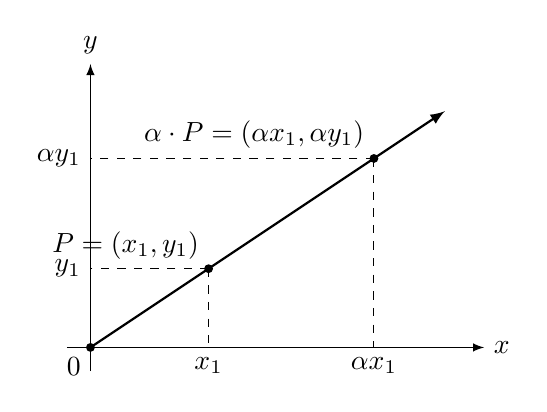
\begin{tikzpicture}[>=latex]
  \draw[->] (-0.3,0) -- (5.0,0) node[right]{$x$};
  \draw[->] (0,-0.3) -- (0,3.6) node[above]{$y$};
  \fill (0,0) circle (1.6pt) node[below left]{$0$};
  \coordinate (P) at (1.5,1.0);
  \coordinate (aP) at (3.6,2.4);
  \draw[dashed] (P) -- (1.5,0) node[below]{$x_1$};
  \draw[dashed] (P) -- (0,1.0) node[left]{$y_1$};
  \draw[dashed] (aP) -- (3.6,0) node[below]{$\alpha x_1$};
  \draw[dashed] (aP) -- (0,2.4) node[left]{$\alpha y_1$};
  \draw[thick, ->] (0,0) -- (4.5,3.0);
  \fill (P) circle (1.6pt) node[above left]{$P = (x_1, y_1)$};
  \fill (aP) circle (1.6pt) node[above left]{$\alpha \cdot P = (\alpha x_1, \alpha y_1)$};
\end{tikzpicture}
\end{center}

因此, 点 $P \in E$ 与纯量 $\alpha \in \mathbb{R}$ 的乘法可以解释为以伸缩中心 $0$,伸缩因子 $\alpha$ 的伸缩映射.若把点 $P \in E$ 看作有向线段意义上的"向量" $\overrightarrow{0P}$, 则这一描述尤其富有启发性.于是向量由它的长度和方向刻画(\emph{零向量}(\textup{Nullvektor})\index{lingxiangliang@零向量(Nullvektor)} $\overrightarrow{00}$ 除外, 它没有确定的方向).向量 $\alpha \cdot \overrightarrow{0P}$ 是由 $\overrightarrow{0P}$ 以因子 $\alpha$ 伸缩而得到的, 即把它的长度乘上 $\alpha$(或者更准确地说, 乘上\emph{绝对值}(\textup{Absolutbetrag})\index{jueduizhi@绝对值(Absolutbetrag)} $|\alpha|$), 其余则保持或反转向量的方向, 视 $\alpha \geq 0$ 还是 $\alpha < 0$ 而定:

\begin{center}
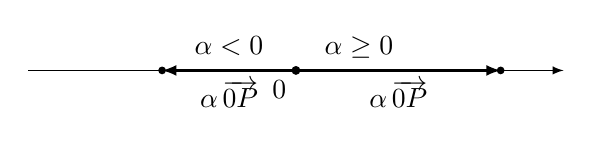
\begin{tikzpicture}[>=latex]
  \draw[->] (-3.4,0) -- (3.4,0);
  \fill (0,0) circle (1.6pt) node[below left]{$0$};
  \draw[thick, ->] (0,0) -- (2.6,0) node[midway,below]{$\alpha\,\overrightarrow{0P}$};
  \fill (2.6,0) circle (1.4pt);
  \draw[thick, ->] (0,0) -- (-1.7,0) node[midway,below]{$\alpha\,\overrightarrow{0P}$};
  \fill (-1.7,0) circle (1.4pt);
  \node[below] at (0.8,0.55) {$\alpha \geq 0$};
  \node[below] at (-0.85,0.55) {$\alpha < 0$};
\end{tikzpicture}
\end{center}

作为另一种运算, 我们考虑 $\mathbb{R}^2$ 中点的加法.对

\[
P_1 = (x_1, y_1), \quad P_2 = (x_2, y_2) \in \mathbb{R}^2
\]

规定

\[
P_1 + P_2 := (x_1 + x_2, y_1 + y_2),
\]

这可在 $E$ 中用如下的草图来说明:

\begin{center}
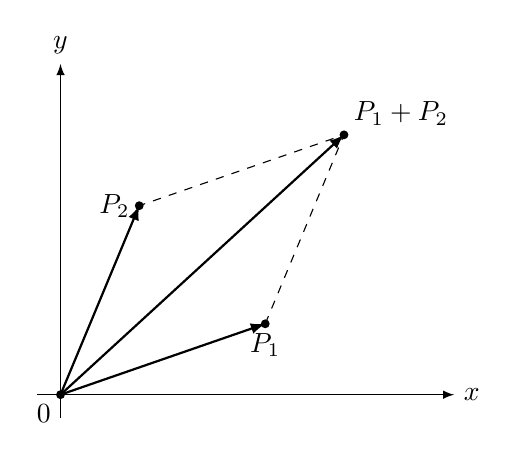
\begin{tikzpicture}[>=latex]
  \draw[->] (-0.3,0) -- (5,0) node[right]{$x$};
  \draw[->] (0,-0.3) -- (0,4.2) node[above]{$y$};
  \fill (0,0) circle (1.6pt) node[below left]{$0$};
  \coordinate (P1) at (2.6,0.9);
  \coordinate (P2) at (1.0,2.4);
  \coordinate (P) at (3.6,3.3);
  \fill (P1) circle (1.6pt) node[below]{$P_1$};
  \fill (P2) circle (1.6pt) node[left]{$P_2$};
  \fill (P) circle (1.6pt) node[above right]{$P_1 + P_2$};
  \draw[thick, ->] (0,0) -- (P1);
  \draw[thick, ->] (0,0) -- (P2);
  \draw[thick, ->] (0,0) -- (P);
  \draw[dashed] (P1) -- (P) -- (P2);
\end{tikzpicture}
\end{center}

同样, 若把向量理解为有向线段, 则 $E$ 中加法的描述也会更富有启发性.不过这里应当允许, 向量作为有向线段可以与自身平行地平移, 从而脱离坐标原点这一天然起点.向量 $\overrightarrow{0P_1}$ 与 $\overrightarrow{0P_2}$ 的和则得到向量 $\overrightarrow{0P}$, 其中 $P$ 是这样得到的终点: 把两个\emph{向量组}(\textup{System von Vektoren})\index{xiangliangzu@向量组(System von Vektoren)}合起来, 即在 $0$ 处接上向量 $\overrightarrow{0P_1}$, 再在 $\overrightarrow{0P_1}$ 的终点 $P_1$ 处接上向量 $\overrightarrow{0P_2}$, 大致如下:

\begin{center}
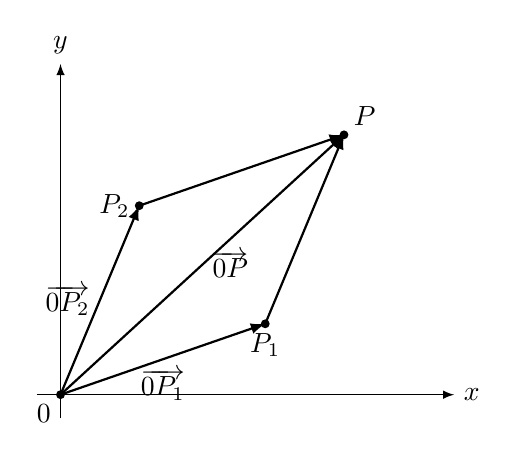
\begin{tikzpicture}[>=latex]
  \draw[->] (-0.3,0) -- (5,0) node[right]{$x$};
  \draw[->] (0,-0.3) -- (0,4.2) node[above]{$y$};
  \fill (0,0) circle (1.6pt) node[below left]{$0$};
  \coordinate (P1) at (2.6,0.9);
  \coordinate (P2) at (1.0,2.4);
  \coordinate (P) at (3.6,3.3);
  \fill (P1) circle (1.6pt) node[below]{$P_1$};
  \fill (P2) circle (1.6pt) node[left]{$P_2$};
  \fill (P) circle (1.6pt) node[above right]{$P$};
  \draw[thick, ->] (0,0) -- (P1) node[midway,below]{$\overrightarrow{0P_1}$};
  \draw[thick, ->] (0,0) -- (P2) node[midway,left]{$\overrightarrow{0P_2}$};
  \draw[thick, ->] (0,0) -- (P) node[midway,right]{$\overrightarrow{0P}$};
  \draw[thick, ->] (P1) -- (P);
  \draw[thick, ->] (P2) -- (P);
\end{tikzpicture}
\end{center}

上述平行四边形构造表明, 如果把向量 $\overrightarrow{0P_2}$ 接在 $0$ 处, 再把向量 $\overrightarrow{0P_1}$ 接在 $\overrightarrow{0P_2}$ 的终点, 加法结果不变.因此向量的加法不依赖于加数的次序, 它是交换的.

我们把 $\mathbb{R}^2$ 的\emph{元素}(\textup{Element})\index{yuansu@元素(Element)}一方面解释为点, 另一方面也解释为有向线段意义上的(可平移的)向量, 这也许会使人有些困惑.原则上, 可以把点与向量的概念加以区分, 办法是把赋给点 $\mathcal{P} \in \mathbb{R}^2$ 的向量 $\overrightarrow{0P}$ 解释为平移 $Q \longmapsto P + Q$, 即 $\mathbb{R}^2$ 到自身的,把元素 $Q \in \mathbb{R}^2$ 映射为 $P + Q$ 的映射.不过我们不打算利用这种可能性, 因为对我们来说, 区分这些概念不会带来好处, 只会把事情复杂化.

接下来我们要说明, $\mathbb{R}^2$ 或 $E$ 中点和向量的加法还会自然地诱导出减法.对 $P_0 = (x_0, y_0) \in \mathbb{R}^2$, 规定

\[
-P_0 = -(x_0, y_0) := (-1) \cdot (x_0, y_0) = (-x_0, -y_0),
\]

并称之为 $P_0$ 的负元素或\emph{逆元}(\textup{inverses Element})\index{niyuan@逆元(inverses Element)}素.它被唯一地表征为满足方程 $P_0 + Q = 0$ 的元素 $Q \in \mathbb{R}^2$.两个元素 $P_1 = (x_1, y_1)$ 与 $P_0 = (x_0, y_0)$ 在 $\mathbb{R}^2$ 中的减法于是很自然地归结为加法:

\[
P_1 - P_0 := P_1 + (-P_0) = (x_1 - x_0, y_1 - y_0).
\]

若再次采用 $E$ 中的向量观点, 那么 $-\overrightarrow{0P_0}$ 由向量 $\overrightarrow{0P_0}$ 反转方向而得到, 其长度保持不变.于是两个向量 $\overrightarrow{0P_1}$ 与 $\overrightarrow{0P_0}$ 的差可以如下表示:

\begin{center}
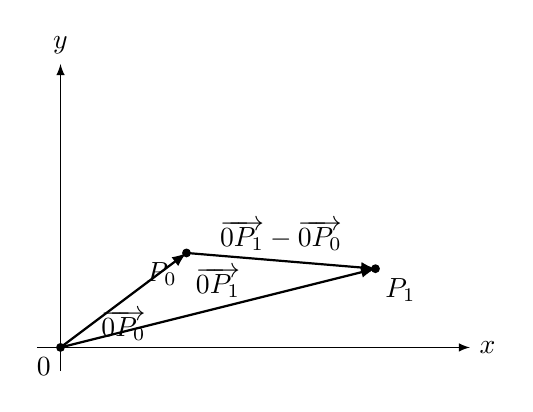
\begin{tikzpicture}[>=latex]
  \draw[->] (-0.3,0) -- (5.2,0) node[right]{$x$};
  \draw[->] (0,-0.3) -- (0,3.6) node[above]{$y$};
  \fill (0,0) circle (1.6pt) node[below left]{$0$};
  \coordinate (P0) at (1.6,1.2);
  \coordinate (P1) at (4.0,1.0);
  \fill (P0) circle (1.6pt) node[below left]{$P_0$};
  \fill (P1) circle (1.6pt) node[below right]{$P_1$};
  \draw[thick, ->] (0,0) -- (P1) node[midway,above]{$\overrightarrow{0P_1}$};
  \draw[thick, ->] (0,0) -- (P0) node[midway,below]{$\overrightarrow{0P_0}$};
  \draw[thick, ->] (P0) -- (P1) node[midway,above]{$\overrightarrow{0P_1} - \overrightarrow{0P_0}$};
\end{tikzpicture}
\end{center}

特别可以看出, 向量 $\overrightarrow{0P_0}$ 与 $\overrightarrow{0P_1} - \overrightarrow{0P_0}$ 的和恰好等于向量 $\overrightarrow{0P_1}$, 这正是合理定义的加法与减法理应做到的.更一般地, 可以作具有如下形式的和

\[
\overrightarrow{0P} = \overrightarrow{0P_0} + \alpha \cdot (\overrightarrow{0P_1} - \overrightarrow{0P_0})
\]

其中 $\alpha \in \mathbb{R}$ 取不同的值.当 $P_0 \neq P_1$ 时, 点 $P$ 总位于由 $P_0$ 和 $P_1$ 确定的直线 $G$ 上, 并且当 $\alpha$ 遍历 $\mathbb{R}$ 时 $P$ 恰好跑遍 $G$:

\begin{center}
\begin{tikzpicture}[>=latex]
  \draw[->] (-0.5,0) -- (5.4,0) node[right]{$x$};
  \draw[->] (0,-0.4) -- (0,3.8) node[above]{$y$};
  \fill (0,0) circle (1.6pt) node[below left]{$0$};
  \coordinate (P0) at (1.4,1.6);
  \coordinate (P1) at (3.8,1.2);
  \coordinate (P) at (2.6,1.4);
  \fill (P0) circle (1.6pt) node[below left]{$P_0$};
  \fill (P1) circle (1.6pt) node[below right]{$P_1$};
  \fill (P) circle (1.6pt) node[above]{$P$};
  \draw[thick] (0.8,1.7) -- (4.4,1.1);
  \node[right] at (4.4,1.1) {$G$};
\end{tikzpicture}
\end{center}

于是, $E$ 或 $\mathbb{R}^2$ 中过给定点 $P_0$ 与 $P_1$ 的直线由方程

\[
G = \{P_0 + t \cdot (P_1 - P_0);\; t \in \mathbb{R}\}
\]

描述.若给定两条这样的直线

\[
G = \{P_0 + t \cdot (P_1 - P_0);\; t \in \mathbb{R}\}, \qquad
G' = \{P_0' + t \cdot (P_1' - P_0');\; t \in \mathbb{R}\}
\]

其中 $P_0 \neq P_1$, $P_0' \neq P_1'$, 那么它们平行当且仅当 $P_1 - P_0$ 是 $P_1' - P_0'$ 的纯量倍(或反之, $P_1' - P_0'$ 是 $P_1 - P_0$ 的纯量倍).若不平行, 则 $G$ 与 $G'$ 恰有一个交点, 而这个交点的计算归结为所谓\emph{线性方程组}(\textup{lineares Gleichungssystem})\index{xianxingfangchengzu@线性方程组(lineares Gleichungssystem)}的求解, 该方程组由 $2$ 个方程,$2$ 个未知数(即 $G$ 与 $G'$ 交点的坐标)组成.这类方程组的求解, 我们将在第 3 章中详细处理.

上述这些考虑可以毫无困难地推广到三维空间及其模型 $\mathbb{R}^3$.例如, 对两点 $P_0, P_1 \in \mathbb{R}^3$, 再次有

\[
G = \{P_0 + t \cdot (P_1 - P_0);\; t \in \mathbb{R}\}
\]

是 $\mathbb{R}^3$ 中由 $P_0$ 和 $P_1$ 确定的直线.对点 $P_0, P_1, P_2 \in \mathbb{R}^3$, 令 $P_1' := P_1 - P_0$, $P_2' := P_2 - P_0$, 相应地可考虑如下图形:

\[
E = \{P_0 + s \cdot P_1' + t \cdot P_2';\; s, t \in \mathbb{R}\}.
\]

\begin{center}
\begin{tikzpicture}[>=latex, line cap=round, x={(0.86cm,0.4cm)}, y={(-0.86cm,0.4cm)}, z={(0,1cm)}]
  \draw[->] (0,0,0) -- (4.2,0,0) node[below]{$x$};
  \draw[->] (0,0,0) -- (0,4.2,0) node[right]{$y$};
  \draw[->] (0,0,0) -- (0,0,4.2) node[above]{$z$};
  \fill (0,0,0) circle (1.5pt) node[below]{$0$};
  \coordinate (P0) at (1,1,0.5);
  \coordinate (P1) at (2.8,1.6,0.8);
  \coordinate (P2) at (1.5,2.6,1.8);
  \coordinate (Q) at (3.3,3.2,2.1);
  \draw (P0) -- (P1) -- (Q) -- (P2) -- cycle;
  \draw[thick, ->] (P0) -- (P1) node[midway,below]{$P_1'$};
  \draw[thick, ->] (P0) -- (P2) node[midway,left]{$P_2'$};
  \fill (P0) circle (1.5pt) node[below left]{$P_0$};
  \fill (P1) circle (1.5pt) node[right]{$P_1$};
  \fill (P2) circle (1.5pt) node[above]{$P_2$};
\end{tikzpicture}
\end{center}

如果 $P_1'$ 不是 $P_2'$ 的倍数,$P_2'$ 也不是 $P_1'$ 的倍数, 即把这两个向量接在 $0$ 处时不位于过 $0$ 的同一条直线上, 那么就称 $P_1'$ 与 $P_2'$ \emph{线性无关}(\textup{linear unabhängig})\index{xianxingwuguan@线性无关(linear unabhängig)}.在这种情况下把 $E$ 认作平面, 否则认作直线, 甚至只是一个点.由于这里向量 $P_1'$ 与 $P_2'$ 起着决定性的作用, 我们还应当考虑如下图形:

\[
E' = \{s \cdot P_1' + t \cdot P_2';\; s, t \in \mathbb{R}\},
\]

它是由 $E$ 沿向量 $-\overrightarrow{0P_0}$ 平移而得到的:

\begin{center}
\begin{tikzpicture}[>=latex, line cap=round, x={(0.86cm,0.4cm)}, y={(-0.86cm,0.4cm)}, z={(0,1cm)}]
  \draw[->] (0,0,0) -- (4.2,0,0) node[below]{$x$};
  \draw[->] (0,0,0) -- (0,4.2,0) node[right]{$y$};
  \draw[->] (0,0,0) -- (0,0,4.2) node[above]{$z$};
  \fill (0,0,0) circle (1.5pt) node[below]{$0$};
  \coordinate (P1) at (1.8,0.6,0.3);
  \coordinate (P2) at (0.5,1.6,1.3);
  \coordinate (Q) at (2.3,2.2,1.6);
  \draw (0,0,0) -- (P1) -- (Q) -- (P2) -- cycle;
  \draw[thick, ->] (0,0,0) -- (P1) node[midway,below]{$P_1'$};
  \draw[thick, ->] (0,0,0) -- (P2) node[midway,left]{$P_2'$};
  \fill (P1) circle (1.5pt) node[right]{$P_1'$};
  \fill (P2) circle (1.5pt) node[above]{$P_2'$};
\end{tikzpicture}
\end{center}

在向量空间的框架中, 称 $E'$ 为 $\mathbb{R}^3$ 中由 $P_1'$ 与 $P_2'$ 张成或生成的\emph{线性子空间}(\textup{linearer Unterraum; Untervektorraum})\index{xianxingzikongjian@线性子空间(linearer Unterraum; Untervektorraum)}.更一般地, 可以在 $\mathbb{R}^3$ 中考虑由任意多个向量 $Q_1, \ldots, Q_r$ 生成的线性子空间

\[
U = \{t_1 Q_1 + \cdots + t_r Q_r;\; t_1, \ldots, t_r \in \mathbb{R}\}.
\]

对于向量 $Q \in \mathbb{R}^3$, 若 $Q \in U$, 则说 $Q$ 线性地依赖于 $Q_1, \ldots, Q_r$.可能出现如下情形: 若 $Q_1 = \cdots = Q_r = 0$, 则 $U$ 只由原点 $0$ 组成.但若 $Q_1, \ldots, Q_r$ 中有某个向量非零, 例如 $Q_1 \neq 0$, 那么 $U$ 至少包含由 $Q_1$ 确定的直线 $G = \{t Q_1;\; t \in \mathbb{R}\}$.若 $Q_2, \ldots, Q_r$ 也都属于 $G$, 即它们线性依赖于 $Q_1$, 则 $U$ 与 $G$ 一致.若情况不是这样, 例如 $Q_2 \notin G$, 则 $Q_1$ 与 $Q_2$ 张成平面 $E = \{t_1 Q_1 + t_2 Q_2;\; t_1, t_2 \in \mathbb{R}\}$, 因而 $U$ 至少包含这个平面.若 $Q_3, \ldots, Q_r \in E$, 即它们线性依赖于 $Q_1, Q_2$, 则 $U$ 与 $E$ 一致.否则在这些向量中有一个, 例如 $Q_3$, 不属于 $E$.于是向量 $Q_1, Q_2, Q_3$ 可以说构成了 $\mathbb{R}^3$ 中的一个坐标系, 而且我们看到 $U$ 与整个 $\mathbb{R}^3$ 一致, 也就是说 $\mathbb{R}^3$ 中一切向量都线性依赖于 $Q_1, Q_2, Q_3$.特别得到: $\mathbb{R}^3$ 中的线性子空间要么由原点组成, 要么由过 $0$ 的直线,过 $0$ 的平面组成, 要么等于整个 $\mathbb{R}^3$.

刚刚引入的向量\emph{线性相关}(\textup{linear abhängig})\index{xianxingxiangguan@线性相关(linear abhängig)}性的概念是一个十分\emph{核}(\textup{Kern})\index{he@核(Kern)}心的要点, 本章将在向量空间的框架内对它进行详细的处理.在这里, 称一个向量组 $Q_1, \ldots, Q_r$ 线性无关, 如果其中每个向量都不线性依赖于其余的向量.上面所做的考察表明, 例如 $\mathbb{R}^3$ 中线性无关的向量组至多由 $3$ 个元素组成.特别地, 线性无关的向量组(正如我们在上述 $\mathbb{R}^3$ 的线性子空间的例子中所构造的那样)将使我们能够在向量空间的语境下精确刻画坐标系或\emph{维数}(\textup{Dimension})\index{weishu@维数(Dimension)}的概念.作为向量线性无关组的推广, 我们最后还将研究向量空间的线性子空间所谓\emph{直和}(\textup{direkte Summe})\index{zhihe@直和(direkte Summe)}.

到目前为止, 关于向量空间我们只考虑了 $n = 1, 2, 3$ 的模型 $\mathbb{R}^n$, 我们的几何想象力在很大程度上参与了论证.在随后各节处理向量空间时, 我们将采取更彻底的方式, 允许一系列推广, 并且在发展理论时只依赖某些公理化的基础.首先, 我们不再把底层纯量的范围限制为实数 $\mathbb{R}$, 而是允许任意\emph{域}(\textup{Körper})\index{yu@域(Körper)}.域可以看作带有某些关于加法与乘法公理的数字系统, 这些公理本质上与实数运算的规则一致.因此, 除了实数域 $\mathbb{R}$ 之外, 人们还知道有理数域 $\mathbb{Q}$ 以及\emph{复数域}(\textup{Körper der komplexen Zahlen})\index{fushuyu@复数域(Körper der komplexen Zahlen)} $\mathbb{C}$.但也有只含有限多个元素的域.

域的公理建立在\emph{群}(\textup{Gruppe})\index{qun@群(Gruppe)}公理之上, 因为一个域连同其加法尤其构成一个群.因此, 在本章中, 经过关于集合的某些准备之后, 我们将首先从相应的群公理出发研究群.然后我们继续讨论域及其运算规则, 进而达到向量空间.向量空间总要与相应的纯量范围, 即与之相关的域联系起来; 人们称之为一个域 $K$ 上的向量空间, 或 $K$-向量空间.一个 $K$-向量空间 $V$ 配备有加法与数乘, 即对 $a, b \in V$ 和 $\alpha \in K$, 和 $a + b$ 以及\emph{数积}(\textup{skalares Produkt})\index{shuji@数积(skalares Produkt)} $\alpha \cdot a$ 都作为 $V$ 的元素而定义.加法与数乘满足所谓向量空间公理, 这些公理关于加法尤其包含群公理.$K$-向量空间的原型是: 对给定的自然数 $n$, 集合

\[
K^n = \{(a_1, \ldots, a_n);\; a_1, \ldots, a_n \in K\}
\]

即一切以 $K$ 中元素为分量的 $n$ 元组的全体, 其中加法与数乘由

\[
\begin{array}{c}
(a_1, \ldots, a_n) + (b_1, \ldots, b_n) := (a_1 + b_1, \ldots, a_n + b_n), \\
\alpha \cdot (a_1, \ldots, a_n) := (\alpha a_1, \ldots, \alpha a_n)
\end{array}
\]

给出.

特别地, 这一定义把上面提到的 $n = 1, 2, 3$ 时的一串模型 $\mathbb{R}^n$ 推广到了任意维数 $n$.这确实有着现实背景: 例如要描述三维空间中一个粒子随时间的变化, 除了 $3$ 个空间坐标之外还需要一个额外的时间坐标, 因而实际上是在向量空间 $\mathbb{R}^4$ 中运动.类似地, 三维空间中两点的对可以被刻画为 $\mathbb{R}^6$ 中的点.

\section{集合与映射}\label{sec:1.1}

通常在这里应当从严格的集合论公理体系开始.但这样做需要不相称的巨大工作量, 因此我们在此满足于一个朴素的立场: 把集合仅仅理解为某些对象--即所谓该集合的元素--的汇集.一个集合 $X$ 因而由它的元素以唯一的方式确定, 当 $x$ 是 $X$ 的一个元素时我们记 $x \in X$, 否则记 $x \notin X$.特别地, 我们自然地把下列集合视为已知:

\[
\begin{array}{r l}
\emptyset = \text{空集}, & \mathbb{N} = \{0, 1, 2, \ldots\}\ \text{自然数}, \\
\mathbb{Z} = \{0, \pm 1, \pm 2, \ldots\}\ \text{整数}, & \mathbb{Q} = \{p/q;\; p, q \in \mathbb{Z},\ q \neq 0\}\ \text{有理数}, \\
\mathbb{R} = \text{实数}. &
\end{array}
\]

这里要指出, 当我们以列举的方式给出一个集合, 例如 $X = \{x_1, \ldots, x_n\}$ 时, 元素 $x_1, \ldots, x_n$ 未必两两不同.这一约定对无穷集合同样适用; 例如可对照上面关于 $\mathbb{Q}$ 的描述.

为了避免矛盾, 集合论公理的设计使得集合的构造要受到一定的限制.例如, 一个集合绝不能把自己作为元素包含在内, 因而全体集合的总体不能被视为一个集合, 因为它会把自己作为元素包含进去.罗素(Russel)悖论提供了与这一问题相关的警示: 我们天真地假设, 全体不含自身的集合, 即

\[
X = \{\text{集合 } A \text{ 且 } A \notin A\},
\]

可以被视为一个集合.那么问 $X \in X$ 是否成立: 在 $X \in X$ 的情形下按 $X$ 的定义立刻得到 $X \notin X$, 而在 $X \notin X$ 的情形下相应地得到 $X \in X$.于是 $X \in X$ 与 $X \notin X$ 同时成立, 这是没有意义的.

对于集合的运用, 重要的是下面这些允许的集合构造过程.

\begin{enumerate}
\item[(1)] \textbf{子集.}--设 $X$ 是一个集合, $P(x)$ 是一个对元素 $x \in X$ 可检验其有效性(真或假)的命题.那么称 $Y = \{x \in X;\; P(x) \text{ 为真}\}$ 为 $X$ 的一个\emph{子集}(\textup{Teilmenge})\index{ziji@子集(Teilmenge)}, 并记 $Y \subset X$.这里也允许 $Y = X$.但若 $Y \neq X$, 则称 $Y$ 为 $X$ 的真子集.例如 $\mathbb{R}_{>0} := \{x \in \mathbb{R};\; x > 0\}$ 是 $\mathbb{R}$ 的一个(真)子集.对给定的集合 $X$, $X$ 的子集又构成一个集合, 即所谓\emph{幂集}(\textup{Potenzmenge})\index{miji@幂集(Potenzmenge)} $\mathfrak{P}(X)$.

\item[(2)] \textbf{并集与交集.}--设 $X$ 是一个集合, $I$ 是一个指标集, 即一个其元素将被我们用为指标的集合.若对每个 $i \in I$ 都给定了子集 $X_i \subset X$, 则称

\[
\bigcup_{i \in I} X_i := \{x \in X;\; \text{存在 } i \in I \text{ 使得 } x \in X_i\}
\]

为集合 $X_i,\ i \in I$ 的\emph{并集}(\textup{Vereinigung})\index{bingji@并集(Vereinigung)}, 而

\[
\bigcap_{i \in I} X_i := \{x \in X;\; x \in X_i \text{ 对一切 } i \in I\}
\]

为这些集合的\emph{交集}(\textup{Durchschnitt})\index{jiaoji@交集(Durchschnitt)}, 在两种情形下我们都得到 $X$ 的一个子集.在指标集为有限 $I = \{1, \ldots, n\}$ 的情形下, 也写 $X_1 \cup \cdots \cup X_n$ 代替 $\bigcup_{i \in I} X_i$, 以及 $X_1 \cap \cdots \cap X_n$ 代替 $\bigcap_{i \in I} X_i$.两个子集 $X', X'' \subset X$ 的并集尤其可以写成

\[
X' \cup X'' = \{x \in X;\; x \in X' \text{ 或 } x \in X''\},
\]

这里使用的是不排除性的数学"或", 即也允许 $x \in X'$ 与 $x \in X''$ 同时成立, 从而 $x \in X' \cap X''$.此外, 当两个子集 $X', X'' \subset X$ 的交集为空, 即 $X' \cap X'' = \emptyset$ 时, 称它们为\emph{不相交的}(\textup{disjunkt})\index{buxiangjiaode@不相交的(disjunkt)}.作为集合 $X_i,\ i \in I$ 的并集的一个变体, 可以构造它们的\emph{无交并}(\textup{disjunkte Vereinigung})\index{wujiaobing@无交并(disjunkte Vereinigung)} $\bigsqcup_{i \in I} X_i$.它是指属于某个 $X_i$ 的一切元素的总体, 不过对不同的指标 $i, j \in I$, $X_i$ 的元素被看作与 $X_j$ 的一切元素不同.

\item[(3)] \textbf{差集.}--若 $X_1, X_2$ 是集合 $X$ 的子集, 则称

\[
X_1 - X_2 := \{x \in X_1;\; x \notin X_2\}
\]

为 $X_1$ 与 $X_2$ 的差集.这又是 $X$ 的一个子集, 甚至是 $X_1$ 的子集.

\item[(4)] \textbf{集合的笛卡尔积.}--设 $X_1, \ldots, X_n$ 是集合.则称

\[
\prod_{i = 1}^{n} X_i := \{(x_1, \ldots, x_n);\; x_1 \in X_1, \ldots, x_n \in X_n\}
\]

为集合 $X_1, \ldots, X_n$ 的\emph{笛卡尔积}(\textup{kartesisches Produkt})\index{dikaerji@笛卡尔积(kartesisches Produkt)}, 其中也使用记号 $X_1 \times \cdots \times X_n$, 若 $X_1 = \cdots = X_n = X$ 则记 $X^n$.元素 $(x_1, \ldots, x_n)$ 称为以 $x_i \in X_i$ 为分量的 $n$ 元组.对两个 $n$ 元组, 恰好当 $x_i = x_i'$ 对 $i = 1, \ldots, n$ 成立时, 才有 $(x_1, \ldots, x_n) = (x_1', \ldots, x_n')$.类似地, 对指标集 $I$, 也可以作给定集合 $X_i,\ i \in I$ 的笛卡尔积 $\prod_{i \in I} X_i$.这种乘积的元素写成元素\emph{族}(\textup{Familie})\index{zu@族(Familie)} $(x_i)_{i \in I}$, 其中 $x_i \in X_i$, 它们指用 $I$ 来指标化的元组.若诸 $X_i$ 都是同一个集合 $X$ 的副本, 则用 $X^I$ 代替 $\prod_{i \in I} X_i$.由空指标集 $I = \emptyset$ 指标化的族 $(x_i)_{i \in \emptyset}$ 称为空族.因此, 在 $I = \emptyset$ 的情形下, 笛卡尔积 $\prod_{i \in I} X_i$ 和 $X^I$ 恰好由一个元素组成, 即空族.
\end{enumerate}

下面我们接着谈集合之间的映射概念.

\begin{definition}[映射]\label{def:1.1.1}\index{yingshe@映射(Abbildung)}
两个集合 $X$ 与 $Y$ 之间的一个映射 $f \colon X \longrightarrow Y$ 是一条规则, 它给每个 $x \in X$ 指派一个完全确定的元素 $y \in Y$, 记为 $f(x)$; 此时也写 $x \longmapsto f(x)$.这里称 $X$ 为映射 $f$ 的\emph{定义域}(\textup{Definitionsbereich})\index{dingyiyu@定义域(Definitionsbereich)}, $Y$ 为 $f$ 的\emph{像域}(\textup{Bildbereich})\index{xiangyu@像域(Bildbereich)}或\emph{值域}(\textup{Wertebereich})\index{zhiyu@值域(Wertebereich)}.
\end{definition}

对集合 $X$ 总存在\emph{恒等映射}(\textup{identische Abbildung})\index{hengdengyingshe@恒等映射(identische Abbildung)} $\operatorname{id} \colon X \longrightarrow X,\ x \longmapsto x$.此外, 例如 $X^I$ 型的笛卡尔积也可以解释为一切映射 $I \longrightarrow X$ 的集合.

以下仍设 $f \colon X \longrightarrow Y$ 是两个集合之间的映射.若 $g \colon Y \longrightarrow Z$ 是另一个映射, 则可以把 $f$ 与 $g$ 复合; 得到的结果是映射

\[
g \circ f \colon X \longrightarrow Z, \quad x \longmapsto g(f(x)).
\]

对子集 $M \subset X$ 与 $N \subset Y$, 称

\[
f(M) := \{y \in Y;\; \text{存在 } x \in M \text{ 使得 } y = f(x)\}
\]

为 $M$ 在 $f$ 下的像, 以及

\[
f^{-1}(N) := \{x \in X;\; f(x) \in N\}
\]

为 $N$ 在 $f$ 下的\emph{原像}(\textup{Urbild})\index{yuanxiang@原像(Urbild)}; 它们分别是 $Y$ 和 $X$ 的子集.若 $N$ 只由一个元素 $y$ 组成, 即 $N = \{y\}$, 则写 $f^{-1}(y)$ 代替 $f^{-1}(\{y\})$.进一步, 若由 $x, x' \in X$ 且 $f(x) = f(x')$ 恒可推出 $x = x'$, 则称 $f$ 为\emph{单射}(\textup{injektiv; injektive Abbildung})\index{danshe@单射(injektiv; injektive Abbildung)}的; 若对每个 $y \in Y$ 都存在 $x \in X$ 使得 $f(x) = y$, 则称 $f$ 为\emph{满射}(\textup{surjektiv; surjektive Abbildung})\index{manshe@满射(surjektiv; surjektive Abbildung)}的.最后, 若 $f$ 既是单射又是满射, 则称 $f$ 为\emph{双射}(\textup{bijektiv; bijektive Abbildung})\index{shuangshe@双射(bijektiv; bijektive Abbildung)}的.

可以说, $f$ 为单射当且仅当每个点 $y \in Y$ 的原像 $f^{-1}(y)$ 要么为空, 要么恰好由一个点 $x \in X$ 组成.又 $f$ 为满射当且仅当对每个 $y \in Y$ 原像 $f^{-1}(y)$ 非空.因此 $f$ 为双射当且仅当对每个元素 $y \in Y$, 原像 $f^{-1}(y)$ 恰好由一个点 $x$ 组成.此时可以对 $f$ 考虑所谓的\emph{逆映射}(\textup{Umkehrabbildung})\index{niyingshe@逆映射(Umkehrabbildung)} $g \colon Y \longrightarrow X$.它给点 $y \in Y$ 指派唯一确定的元素 $x \in f^{-1}(y)$, 并且有 $g \circ f = \operatorname{id}_X$ 与 $f \circ g = \operatorname{id}_Y$.对映射 $f \colon X \longrightarrow Y$, 只要它存在, 其逆映射通常记为 $f^{-1} \colon Y \longrightarrow X$.

\aufgaben

\noindent 设 $A, B, C$ 是集合 $X$ 的子集.证明:
\begin{enumerate}
\item[(i)] $A \cap (B \cup C) = (A \cap B) \cup (A \cap C)$;
\item[(ii)] $A \cup (B \cap C) = (A \cup B) \cap (A \cup C)$;
\item[(iii)] $A - (B \cup C) = (A - B) \cap (A - C)$;
\item[(iv)] $A - (B \cap C) = (A - B) \cup (A - C)$.
\end{enumerate}

\medskip
\noindent\textbf{习题 2.} 设 $f \colon X \longrightarrow Y$ 是集合之间的一个映射.对子集 $M_1, M_2 \subset X$ 与 $N_1, N_2 \subset Y$ 证明:
\begin{enumerate}
\item[(i)] $f(M_1 \cup M_2) = f(M_1) \cup f(M_2)$;
\item[(ii)] $f(M_1 \cap M_2) \subset f(M_1) \cap f(M_2)$;
\item[(iii)] $f^{-1}(N_1 \cup N_2) = f^{-1}(N_1) \cup f^{-1}(N_2)$;
\item[(iv)] $f^{-1}(N_1 \cap N_2) = f^{-1}(N_1) \cap f^{-1}(N_2)$.
\end{enumerate}
在 (ii) 中甚至成立等式吗?

\medskip
\noindent\textbf{习题 3.} 设 $X \xrightarrow{\ f\ } Y \xrightarrow{\ g\ } X$ 是满足 $g \circ f = \operatorname{id}$ 的集合映射.证明 $f$ 是单射, $g$ 是满射.

\medskip
\noindent\textbf{习题 4.}
\begin{enumerate}
\item[(i)] 存在双射 $\mathbb{N} \longrightarrow \mathbb{Z}$ 吗?
\item[(ii)] 对 $n \in \mathbb{N}$, 存在双射 $\mathbb{N} \longrightarrow \mathbb{N} \times \{1, \ldots, n\}$ 吗?
\item[(iii)] 存在双射 $\mathbb{N} \longrightarrow \mathbb{N} \times \mathbb{N}$ 吗?
\item[(iv)] 存在双射 $\mathbb{N} \longrightarrow \mathbb{Q}$ 吗?
\end{enumerate}

\medskip
\noindent\textbf{习题 5.} 设 $X$ 是一个集合, $f \colon X \longrightarrow \mathfrak{P}(X)$ 是从 $X$ 到其幂集的映射.证明 $f$ 不可能是满射.

\section{群}\index{qun@群(Gruppe)}\label{sec:1.2}

集合 $M$ 上的一个\emph{内运算}(\textup{innere Verknüpfung})\index{neiyunsuan@内运算(innere Verknüpfung)}是指一个映射 $f \colon M \times M \longrightarrow M$.它给 $M$ 中元素的每个对 $(a, b)$ 指派一个元素 $f(a, b) \in M$.为了在记号上也体现运算的\emph{特征}(\textup{Charakteristik})\index{tezheng@特征(Charakteristik)}, 我们将主要写 $a \cdot b$ 代替 $f(a, b)$.对于交换运算, 即对所有 $a, b \in M$ 满足 $f(a, b) = f(b, a)$ 的运算, 我们使用加法的写法 $a + b$.

\begin{definition}[群]\label{def:1.2.1}\index{qun@群(Gruppe)}
一个带内运算 $G \times G \longrightarrow G$, $(a, b) \longmapsto a \cdot b$ 的集合 $G$ 称为一个群, 如果满足下列性质:
\begin{enumerate}
\item[(i)] 运算是结合的, 即对一切 $a, b, c \in G$ 有 $(a \cdot b) \cdot c = a \cdot (b \cdot c)$.
\item[(ii)] 存在一个\emph{单位}(\textup{Einheit; invertierbares Element})\index{danwei@单位(Einheit; invertierbares Element)}元 $e$ 于 $G$ 中, 即一个满足 $e \cdot a = a \cdot e = a$ 对一切 $a \in G$ 成立的元素 $e \in G$.
\item[(iii)] 对每个 $a \in G$ 存在一个逆元, 即一个满足 $a \cdot b = b \cdot a = e$ 的元素 $b \in G$.这里 $e$ 是 (ii) 中所存在的(唯一确定的) $G$ 的单位元.
\end{enumerate}
\end{definition}

若运算是交换的, 即还满足
\begin{enumerate}
\item[(iv)] 对一切 $a, b \in G$ 有 $a \cdot b = b \cdot a$,
\end{enumerate}
则称该群为交换群或\emph{阿贝尔群}(\textup{abelsche Gruppe; kommutative Gruppe})\index{abeierqun@阿贝尔群(abelsche Gruppe; kommutative Gruppe)}.

在上述情形下, 人们通常只简单地说 $G$ 是一个群, 而不明确提及运算"$\cdot$".群的例子有:
\begin{enumerate}
\item[(1)] $\mathbb{Z}$ 关于加法"$+$";
\item[(2)] $\mathbb{Q}$ 关于加法"$+$", 以及 $\mathbb{Q}^* := \mathbb{Q} - \{0\}$ 关于乘法"$\cdot$";
\item[(3)] $\mathbb{R}$ 关于加法"$+$", 以及 $\mathbb{R}^* := \mathbb{R} - \{0\}$ 关于乘法"$\cdot$";
\item[(4)] 对集合 $X$, 双射 $X \longrightarrow X$ 的集合 $\operatorname{Bij}(X, X)$ 以\emph{映射的复合}(\textup{Komposition von Abbildungen})\index{yingshedefuhe@映射的复合(Komposition von Abbildungen)}为运算构成一个群.容易验证, 只要 $X$ 至少含有 $3$ 个不同的元素, 这个群就不是交换的.
\end{enumerate}

正如已经断言的那样, 在一个群 $G$ 中单位元 $e$ 是唯一确定的.事实上, 若 $e' \in G$ 是另一个单位元, 则 $e = e' \cdot e = e'$.类似地可以证明, 属于元素 $a \in G$ 的逆元 $b \in G$ 是唯一确定的.若 $b' \in G$ 是 $a$ 的另一个逆元, 则

\[
b = e \cdot b = (b' \cdot a) \cdot b = b' \cdot (a \cdot b) = b' \cdot e = b'.
\]

刚才进行的推导(除了 $e$ 和 $b$ 的性质外)只需用到 $e'$ 是左单位元, 即对一切 $a \in G$ 具有性质 $e' \cdot a = a$, 以及 $b'$ 是 $a$ 的左逆元, 即满足方程 $b' \cdot a = e$.相应地也可以对右单位元或右逆元作同样的推理.因此在一个群中, 每个左(或右)单位元都与唯一确定的单位元 $e \in G$ 一致, 因而尤其是右(或左)单位元.类似地可以看出, 左逆元也是右逆元, 右逆元也是左逆元.我们甚至还可以更进一步, 按这个意思削弱群的界定条件:

\begin{remark}[群的界定条件的削弱]\label{rem:1.2.2}\index{qun@群(Gruppe)}
在定义~\mtref{def:1.2.1} 中, 代替 (ii) 和 (iii), 只需要求存在一个具有下列性质的元素 $e \in G$:
\begin{enumerate}
\item[(ii$^-$)] $e$ 在 $G$ 中是左单位元, 即对一切 $a \in G$ 有 $e \cdot a = a$;
\item[(iii$^-$)] 对每个 $a \in G$, 在 $G$ 中存在关于 $e$ 的左逆元, 即一个满足 $b \cdot a = e$ 的元素 $b \in G$.
\end{enumerate}
\end{remark}

\begin{proof}
设 $G$ 是一个带乘法记法运算的集合, 且含有一个元素 $e \in G$, 使得条件 (i),(ii$^-$),(iii$^-$) 成立.为看出 $G$ 是群, 我们必须证明定义~\mtref{def:1.2.1} 的条件 (ii) 和 (iii) 成立.我们首先证明: 对元素 $a \in G$, 每个关于 $e$ 是 $a$ 的左逆元的元素 $b \in G$, 也是关于 $e$ 的右逆元.设 $b \cdot a = e$, 并设 $c$ 是 $b$ 的一个左逆元, 即 $c \cdot b = e$.于是

\[
\begin{array}{r l}
& a \cdot b = (e \cdot a) \cdot b = ((c \cdot b) \cdot a) \cdot b = (c \cdot (b \cdot a)) \cdot b \\
& \qquad = (c \cdot e) \cdot b = c \cdot (e \cdot b) = c \cdot b = e,
\end{array}
\]

所以 $b$ 关于 $e$ 是 $a$ 的右逆元.剩下的还要证明左单位元 $e$ 也是右单位元.设 $a \in G$.若 $b \in G$ 关于 $e$ 是 $a$ 的左逆元, 那么如我们所见, $b$ 关于 $e$ 也是 $a$ 的右逆元, 于是

\[
a \cdot e = a \cdot (b \cdot a) = (a \cdot b) \cdot a = e \cdot a = a,
\]

即 $e$ 是右单位元.
\end{proof}

群 $G$ 的单位元 $e$ 在运算采用乘法写法时通常称为\emph{幺元}(\textup{Einselement; neutrales Element})\index{yaoyuan@幺元(Einselement; neutrales Element)}, 并写 $1$ 代替 $e$.对 $a \in G$ 的逆元使用记号 $a^{-1}$.此外, 在乘法写法的群运算中, 习惯上只要不引起混淆就省略运算\emph{符号}(\textup{Signum})\index{fuhao@符号(Signum)}"$\cdot$".对有限多个元素 $a_1, \ldots, a_n \in G$, 通过

\[
\prod_{i = 1}^{n} a_i := a_1 \cdot \cdots \cdot a_n
\]

定义这些元素的乘积.由于\emph{结合律}(\textup{Assoziativgesetz})\index{jiehelv@结合律(Assoziativgesetz)}, 此处无需特别加括号; 对这一"显然"事实的详细证明我们在此略去.下面我们主要考虑对指标 $n \in \mathbb{N}$ 的有限\emph{序列}(\textup{Sequenz})\index{xulie@序列(Sequenz)} $a_1, \ldots, a_n \in G$, 因而特别允许 $n = 0$ 的情形.这时是空序列, 相应的空积规定为

\[
\prod_{i = 1}^{0} a_i := 1.
\]

如已所说, 对交换运算主要采用加法写法.交换群的单位元写作\emph{零元}(\textup{Nullelement})\index{lingyuan@零元(Nullelement)} $0$, 元素 $a \in G$ 的逆元写作 $-a$.代替 $a + (-a')$ 通常使用记号 $a - a'$.元素 $a_i \in G,\ i = 1, \ldots, n$ 的有限和写成 $\sum_{i = 1}^{n} a_i$ 的形式, 其中空和规定为

\[
\sum_{i = 1}^{0} a_i := 0.
\]

\begin{definition}[\emph{子群}\index{ziqun@子群(Untergruppe)}]\label{def:1.2.3}\index{ziqun@子群(Untergruppe)}
设 $G$ 是一个群.子集 $H \subset G$ 称为 $G$ 的子群, 如果满足:
\begin{enumerate}
\item[(i)] $a, b \in H \Longrightarrow ab \in H$;
\item[(ii)] $1 \in H$;
\item[(iii)] $a \in H \Longrightarrow a^{-1} \in H$.
\end{enumerate}
\end{definition}

若 $H \subset G$ 是一个子群, 则群运算 $G \times G \longrightarrow G$ 限制为 $H \times H \longrightarrow H$ 上的运算, 且 $H$ 关于此运算本身又是一个群.反之, 若后者成立, 则可容易地证明 $H$ 是 $G$ 的子群.此外立刻可见, 非空子集 $H \subset G$ 只要满足条件 $a, b \in H \Longrightarrow ab^{-1} \in H$, 就已是 $G$ 的子群.一个群 $G$ 恒含有平凡子群 $\{1\}$ 和 $G$.

下面我们处理群中运算的一些基本计算规则.对元素 $a, b, c \in G$ 有:

\[
\begin{array}{l l}
(1) & ab = ac \Longrightarrow b = c, \qquad ac = bc \Longrightarrow a = b, \\
(2) & (a^{-1})^{-1} = a, \\
(3) & (ab)^{-1} = b^{-1} a^{-1}.
\end{array}
\qquad \text{(\emph{消去律}(\textup{Kürzungsregeln})\index{xiaoqulv@消去律(Kürzungsregeln)})}
\]

为验证 (1), 分别从左乘以 $a^{-1}$ 或从右乘以 $c^{-1}$ 即可.在情形 (2) 中可如下推理: 如我们所看到的, $(a^{-1})^{-1}$ 是 $G$ 中那个(从左边或右边)乘以 $a^{-1}$ 得到 $1$ 的唯一确定的元素.由于 $a^{-1} a = 1$, 得 $(a^{-1})^{-1} = a$.相应地得到 $(ab)^{-1} = b^{-1} a^{-1}$, 因为 $(b^{-1} a^{-1})(ab) = b^{-1}(a^{-1} a) b = b^{-1} b = 1$.

最后我们还要给出群的一个特殊刻画.

\begin{theorem}[群的刻画]\label{thm:1.2.4}
一个非空集合 $G$ 连同运算 $(a, b) \longmapsto a \cdot b$ 是一个群, 当且仅当满足:
\begin{enumerate}
\item[(i)] 运算是结合的;
\item[(ii)] 对 $a, b \in G$ 总存在元素 $x, y \in G$ 使得 $x \cdot a = b$ 与 $a \cdot y = b$.
\end{enumerate}
若这些条件满足, 则 (ii) 中的元素 $x, y$ 由 $a, b$ 唯一确定.
\end{theorem}

\begin{proof}
若 $G$ 是群, 则把 (ii) 中的等式分别从右或从左乘以 $a^{-1}$.于是 $x = ba^{-1}$ 及 $y = a^{-1}b$ 是唯一确定的解.反之, 设定理的条件满足, 并设 $a \in G$.按 (ii) 存在元素 $e \in G$ 使得 $ea = a$.对 $b \in G$ 又存在 $y \in G$ 使得 $ay = b$, 于是

\[
eb = eay = ay = b,
\]

即 $e$ 是左单位元.再按 (ii) 得出左逆元的存在性.因此按注记~\mtref{rem:1.2.2}, $G$ 是一个群.
\end{proof}

\aufgaben

\noindent\textbf{习题 1.} 对集合 $X$ 考虑双射 $X \longrightarrow X$ 的集合 $\operatorname{Bij}(X, X)$.验证 $\operatorname{Bij}(X, X)$ 关于映射的复合构成一个群, 并证明只要 $X$ 至少含 $3$ 个不同元素, 这个群就不是交换的.

\medskip
\noindent\textbf{习题 2.} 设 $G$ 是一个群, $H \subset G$ 是一个子集.证明: $H$ 是 $G$ 的子群当且仅当 $G$ 的群运算在 $H$ 上诱导出一个运算(即对 $a, b \in H$ 恒有 $ab \in H$), 并且 $H$ 关于这个运算本身又是一个群.

\medskip
\noindent\textbf{习题 3.} 设 $G$ 是一个群, $H \subset G$ 是一个子集.证明 $H$ 是 $G$ 的子群当且仅当满足:
\begin{enumerate}
\item[(i)] $H \neq \emptyset$;
\item[(ii)] $a, b \in H \Longrightarrow ab^{-1} \in H$.
\end{enumerate}

\medskip
\noindent\textbf{习题 4.} 设 $G$ 是一个带有子群 $H_1, H_2 \subset G$ 的群.证明 $H_1 \cup H_2$ 是 $G$ 的子群当且仅当 $H_1 \subset H_2$ 或 $H_2 \subset H_1$.

\medskip
\noindent\textbf{习题 5.} 对一个群 $G$ 考虑映射 $i \colon G \longrightarrow G$, $g \longmapsto g^{-1}$.证明:
\begin{enumerate}
\item[(i)] $i$ 是双射.
\item[(ii)] 若 $A \subset G$ 是满足 $i(A) \subset A$ 的子集, 则已经有 $i(A) = A$; 此时称 $A$ 为对称的.
\item[(iii)] 对每个子集 $A \subset G$, $A \cup i(A)$ 与 $A \cap i(A)$ 都是对称的.
\end{enumerate}

\medskip
\noindent\textbf{习题 6.} 设 $G$ 是一个对一切 $a \in G$ 满足 $a^2 = 1$ 的群.证明 $G$ 是阿贝尔群.

\medskip
\noindent\textbf{习题 7.} 设 $G$ 是一个有限阿贝尔群.则 $\prod_{g \in G} g^2 = 1$.

\medskip
\noindent\textbf{习题 8.} 对 $n \in \mathbb{N} - \{0\}$ 考虑子集 $R_n = \{0, 1, \ldots, n - 1\} \subset \mathbb{N}$.设 $\pi \colon \mathbb{Z} \longrightarrow R_n$ 是把每个整数 $\mathbb{Z}$ 指派为其除以 $n$ 后的非负余数的映射.证明:
\begin{enumerate}
\item[(i)] 在 $R_n$ 上存在唯一确定的运算 $(a, b) \longmapsto a + b$, 使得对 $x, y \in \mathbb{Z}$ 恒有 $\pi(x + y) = \pi(x) + \pi(y)$;
\item[(ii)] $R_n$ 关于这个运算是一个阿贝尔群.
\end{enumerate}

\medskip
\noindent\textbf{习题 9.} 设 $G$ 是一个群.在幂集 $\mathfrak{P}(G)$ 上考虑由

\[
(A, B) \longmapsto A \cdot B = \{a \cdot b \in G;\; a \in A, b \in B\}
\]

给出的运算.证明这个运算是结合的并且存在单位元.$\mathfrak{P}(G)$ 关于这个运算甚至是群吗? 如果不是, 哪些元素 $A \in \mathfrak{P}(G)$ 有逆元?

\section{域}\index{yu@域(Körper)}\label{sec:1.3}

域是一个加法写法下的阿贝尔群, 在它上面还额外定义了具有某些性质的乘法, 其范本是有理数或实数.更准确地说:

\begin{definition}[域]\label{def:1.3.1}\index{yu@域(Körper)}
一个域是一个集合 $K$, 带有两个内运算, 写作加法"$+$"与乘法"$\cdot$", 使得下列条件成立:
\begin{enumerate}
\item[(i)] 加法结合律: $(a + b) + c = a + (b + c)$, 对 $a, b, c \in K$;
\item[(ii)] 加法单位元: 存在一个满足 $0 + a = a$ 对一切 $a \in K$ 成立的元素 $0 \in K$;
\item[(iii)] 加法逆元: 对 $a \in K$ 存在一个满足 $b + a = 0$ 的元素 $b \in K$, 其中 $0$ 如 (ii) 所选;
\item[(iv)] 加法\emph{交换律}(\textup{Kommutativgesetz})\index{jiaohuanlv@交换律(Kommutativgesetz)}: $a + b = b + a$, 对 $a, b \in K$;
\item[(v)] 乘法结合律: $(a \cdot b) \cdot c = a \cdot (b \cdot c)$, 对 $a, b, c \in K$;
\item[(vi)] 乘法单位元: 存在一个满足 $1 \cdot a = a$ 对一切 $a \in K$ 成立的元素 $1 \in K$;
\item[(vii)] 乘法逆元: 对 $a \in K - \{0\}$ 存在一个满足 $b \cdot a = 1$ 的元素 $b \in K$, 其中 $1$ 如 (vi) 所选;
\item[(viii)] 乘法交换律: $a \cdot b = b \cdot a$, 对 $a, b \in K$;
\item[(ix)] \emph{分配律}(\textup{Distributivgesetze})\index{fenpeilv@分配律(Distributivgesetze)}: $a \cdot (b + c) = a \cdot b + a \cdot c$ 与 $(a + b) \cdot c = a \cdot c + b \cdot c$, 对 $a, b, c \in K$;
\item[(x)] $1 \neq 0$.
\end{enumerate}
\end{definition}

在分配律 (ix) 中, 本来应当在右侧把 $a \cdot b$, $a \cdot c$, $b \cdot c$ 各项分别加上括号.但人们约定乘法"$\cdot$"先于加法"$+$", 因而括号可以省略.还要指出, 乘法符号"$\cdot$"与群的情形类似, 经常不写出来.元素 $0, 1 \in K$ 是唯一确定的, 称 $0$ 为 $K$ 的零元, $1$ 为 $K$ 的幺元.

下面我们来处理在域 $K$ 中运算的一些简单计算规则.

\begin{enumerate}
\item[(1)] $0a = a0 = 0$, 对 $a \in K$, 因为
\[
0 = 0a - 0a = (0 + 0)a - 0a = 0a + 0a - 0a = 0a.
\]
\item[(2)] $(-1)a = -a$, 对 $a \in K$, 因为
\[
a + (-1)a = 1a + (-1)a = (1 - 1)a = 0a = 0.
\]
\item[(3)] $(-a)b = a(-b) = -ab$, $(-a)(-b) = ab$, 对 $a, b \in K$; 这利用 (2) 即得.
\item[(4)] 对 $a, b \in K$, 由 $ab = 0$ 已经推出 $a = 0$ 或 $b = 0$.因为若 $ab = 0$ 且 $a \neq 0 \neq b$, 则产生矛盾
\[
1 = abb^{-1}a^{-1} = 0b^{-1}a^{-1} = 0.
\]
\end{enumerate}

因此, 在域中的运算大致可以像人们习惯了的有理数或实数的运算那样进行.不过在这里就要指出与熟悉的数域范本之间的差别.对自然数 $n \in \mathbb{N}$ 与元素 $a \in K$, 习惯上把 $a$ 与自己相加 $n$ 次记为 $n \cdot a$, 其中特别在 $n = 0$ 或 $a = 0$ 时有 $n \cdot a = 0$.进一步, 对负整数 $n$ 规定 $n \cdot a = (-n) \cdot (-a)$.然而, 由 $n \cdot a = 0$ 未必推出 $n = 0$ 或 $a = 0$, 这一点我们将在具体例子中看到.

利用群的概念, 域可以如下更清晰地刻画:

\begin{remark}[域的刻画]\label{rem:1.3.2}\index{yu@域(Körper)}
定义~\mtref{def:1.3.1} 中的条件 (i)--(x) 等价于下列条件:
\begin{enumerate}
\item[(i)] $K$ 关于加法是一个阿贝尔群;
\item[(ii)] $K^* = K - \{0\}$ 关于乘法是一个阿贝尔群;
\item[(iii)] 定义~\mtref{def:1.3.1} 中的分配律 (ix) 成立.
\end{enumerate}
\end{remark}

\begin{proof}
首先显然, 定义~\mtref{def:1.3.1} 中的条件 (i)--(iv) 正是交换加法群的条件.其次, 由上述规则 (4) 推出, 对域 $K$, 子集 $K^* = K - \{0\}$ 关于乘法是封闭的, 并且由 $a \cdot a^{-1} = 1$ 可知, 与元素 $a \in K^*$ 一起, 其逆元 $a^{-1}$ 也属于 $K^*$.于是 $K^*$ 关于乘法是一个阿贝尔群, 因而定义~\mtref{def:1.3.1} 的条件蕴含注记~\mtref{rem:1.3.2} 的条件.

反之, 设注记~\mtref{rem:1.3.2} 的条件满足.要从中推出定义~\mtref{def:1.3.1} 的条件, 只需知道在注记~\mtref{rem:1.3.2} 的情形下, 对一切 $a \in K$ 有关系 $0a = 0 = a0$.而这可以借助分配律以我们上面计算规则同样的方式推出.
\end{proof}

与群的情形类似, 域也有\emph{子域}(\textup{Teilkörper})\index{ziyu@子域(Teilkörper)}的概念.

\begin{definition}[子域]\label{def:1.3.3}\index{ziyu@子域(Teilkörper)}
设 $K$ 是一个域.子集 $L \subset K$ 称为 $K$ 的一个子域, 如果满足:
\begin{enumerate}
\item[(i)] $a, b \in L \Longrightarrow a + b, a \cdot b \in L$;
\item[(ii)] $0, 1 \in L$;
\item[(iii)] $a \in L \Longrightarrow -a \in L$;
\item[(iv)] $a \in L,\ a \neq 0 \Longrightarrow a^{-1} \in L$.
\end{enumerate}
\end{definition}

显然, 子集 $L \subset K$ 是 $K$ 的子域当且仅当 $K$ 上的加法与乘法限制为 $L \times L \longrightarrow L$ 上的运算, 且 $L$ 关于这些运算本身是一个域.域的热知例子是有理数 $\mathbb{Q}$ 和实数 $\mathbb{R}$, 其中 $\mathbb{Q}$ 是 $\mathbb{R}$ 的子域.一个域至少含有 $2$ 个不同的元素, 即加法的单位元和乘法的单位元, 也就是 $0$ 和 $1$.另一方面, 也存在恰好由 $2$ 个元素组成的域 $K$.为此考虑子集 $\{0, 1\} \subset \mathbb{Z}$, 并规定:

\[
\begin{array}{c c c}
0 + 0 = 0, & 0 + 1 = 1 + 0 = 1, & 1 + 1 = 0, \\
0 \cdot 0 = 0, & 0 \cdot 1 = 1 \cdot 0 = 0, & 1 \cdot 1 = 1.
\end{array}
\]

验证域公理可知, $\{0, 1\}$ 上的这些运算确实定义了一个域的结构; 通常记为 $\mathbb{F}_2$.当然 $\mathbb{F}_2$ 不是 $\mathbb{Q}$ 或 $\mathbb{R}$ 的子域, 因为 $2 \cdot 1 = 1 + 1 = 0$, 其中 $2$ 应理解为自然数, 而不是 $\mathbb{F}_2$ 的元素.

下面我们要构造 $\mathbb{R}$ 的包含 $\sqrt{2}$ 的最小子的子域, 其中 $\sqrt{2}$ 是与自身相乘等于 $2$ 的那个正实数.这个域通常记为 $\mathbb{Q}(\sqrt{2})$.首先证明:

\begin{lemma}[$\sqrt{2} \notin \mathbb{Q}$]\label{lem:1.3.4}\index{wulishu@无理数(irrationale Zahl)}
$\sqrt{2} \notin \mathbb{Q}$.
\end{lemma}

\begin{proof}
我们间接地, 即用反证法进行证明, 并假设 $\sqrt{2} \in \mathbb{Q}$, 例如 $\sqrt{2} = p/q$, 其中 $p, q \in \mathbb{Z} - \{0\}$.可以把分数 $p/q$ 看作已约分的.特别是 $p$ 与 $q$ 不同时被 $2$ \emph{整除}(\textup{a teilt b; Teiler})\index{zhengchu@整除(a teilt b; Teiler)}.由方程 $p^2/q^2 = 2$ 得 $p^2 = 2q^2$, 从而 $p^2$ 是偶数.由于奇数的平方恒为奇数, $p$ 也必须是偶数, 例如 $p = 2\tilde{p}$, 其中 $\tilde{p} \in \mathbb{Z}$.于是 $2q^2 = 4\tilde{p}^2$ 即 $q^2 = 2\tilde{p}^2$, 从而同上, $2$ 是 $q$ 的因数.这样 $2$ 既是 $p$ 也是 $q$ 的因数.但这正是我们事先排除的.因此假设 $\sqrt{2} \in \mathbb{Q}$ 导致矛盾, 不能成立, 所以 $\sqrt{2} \notin \mathbb{Q}$.
\end{proof}

作为推论得到:

\begin{lemma}\label{lem:1.3.5}
对 $a, b \in \mathbb{Q}$ 有

\[
a + b\sqrt{2} \neq 0 \Longleftrightarrow a \neq 0 \ \text{或}\ b \neq 0.
\]
\end{lemma}

\begin{proof}
蕴含"$\Rightarrow$"是平凡的.为证反向蕴含"$\Longleftarrow$", 我们再采用反证法: 假设存在数 $a, b \in \mathbb{Q}$ 使得 $a + b\sqrt{2} = 0$, 其中 $a$ 与 $b$ 不全为零.则必有 $a \neq 0 \neq b$, 从而 $\sqrt{2} = -ab^{-1} \in \mathbb{Q}$, 与引理~\mtref{lem:1.3.4} 矛盾.
\end{proof}

现在我们定义 $\mathbb{Q}(\sqrt{2})$ 为 $\mathbb{R}$ 的子集:

\[
\mathbb{Q}(\sqrt{2}) = \{a + b\sqrt{2};\; a, b \in \mathbb{Q}\}.
\]

\begin{theorem}[$\mathbb{Q}(\sqrt{2})$ 是最小子域]\label{thm:1.3.6}\index{ziyu@子域(Teilkörper)}
$\mathbb{Q}(\sqrt{2})$ 是 $\mathbb{R}$ 的一个真子域, 它又包含 $\mathbb{Q}$ 作为真子域.$\mathbb{Q}(\sqrt{2})$ 是 $\mathbb{R}$ 的包含 $\sqrt{2}$ 的最小子域.
\end{theorem}

\begin{proof}
首先证明 $\mathbb{Q}(\sqrt{2})$ 是 $\mathbb{R}$ 的子域.为证 $\mathbb{Q}(\sqrt{2})$ 关于加法与乘法封闭, 考虑元素 $a + b\sqrt{2}$, $a' + b'\sqrt{2} \in \mathbb{Q}(\sqrt{2})$, 其中 $a, b, a', b' \in \mathbb{Q}$.于是

\[
\begin{array}{l l}
(a + b\sqrt{2}) + (a' + b'\sqrt{2}) = (a + a') + (b + b')\sqrt{2} & \in \mathbb{Q}(\sqrt{2}), \\
(a + b\sqrt{2}) \cdot (a' + b'\sqrt{2}) = (aa' + 2bb') + (ab' + a'b)\sqrt{2} & \in \mathbb{Q}(\sqrt{2}),
\end{array}
\]

即定义~\mtref{def:1.3.3} 的条件 (i) 满足.条件 (ii) 同样满足, 因为 $0 = 0 + 0\sqrt{2} \in \mathbb{Q}(\sqrt{2})$, $1 = 1 + 0\sqrt{2} \in \mathbb{Q}(\sqrt{2})$.此外, 与 $a + b\sqrt{2}$ 一起, 其关于加法的逆元 $-(a + b\sqrt{2}) = (-a) + (-b)\sqrt{2}$ 也包含在 $\mathbb{Q}(\sqrt{2})$ 中, 所以定义~\mtref{def:1.3.3} 的条件 (iii) 也满足.

稍微困难的是证明定义~\mtref{def:1.3.3} 的条件 (iv).设 $a + b\sqrt{2} \in \mathbb{Q}(\sqrt{2})$ 非零, 即按引理~\mtref{lem:1.3.5} 有 $a \neq 0$ 或 $b \neq 0$.则 $a - b\sqrt{2} \neq 0$ 同样按引理~\mtref{lem:1.3.5} 成立, 于是可写:

\[
\frac{1}{a + b\sqrt{2}} = \frac{a - b\sqrt{2}}{a^2 - 2b^2} = \frac{a}{a^2 - 2b^2} - \frac{b}{a^2 - 2b^2}\sqrt{2} \in \mathbb{Q}(\sqrt{2}).
\]

总之得到 $\mathbb{Q}(\sqrt{2})$ 是 $\mathbb{R}$ 的一个子域, 而且是真子域, 因为例如 $\sqrt{3}$ 不属于 $\mathbb{Q}(\sqrt{2})$.后者可仿照引理~\mtref{lem:1.3.4} 的证明来论证.此外, $\mathbb{Q}(\sqrt{2})$ 包含有理数域作为真子域, 因为 $\sqrt{2} \notin \mathbb{Q}$.

还剩下要证明 $\mathbb{Q}(\sqrt{2})$ 是 $\mathbb{R}$ 的包含 $\sqrt{2}$ 的最小子域.若首先 $K$ 是 $\mathbb{R}$ 的任意子域, 则 $K$ 必包含一切形如 $n \cdot 1$($n \in \mathbb{Z}$)的元素, 即 $\mathbb{Z} \subset K$.于是 $K$ 还必须包含一切形如 $p/q$($p, q \in \mathbb{Z}$, $q \neq 0$)的分数, 从而包含 $\mathbb{Q}$.因此 $\mathbb{Q}$ 是 $\mathbb{R}$ 的最小子域.若又有 $\sqrt{2} \in K$, 则 $K$ 必包含一切形如 $a + b\sqrt{2}$($a, b \in \mathbb{Q}$)的表达式, 从而包含 $\mathbb{Q}(\sqrt{2})$.所以 $\mathbb{Q}(\sqrt{2})$ 是 $\mathbb{R}$ 的(唯一确定的)包含 $\sqrt{2}$ 的最小子域.
\end{proof}

下面我们从实数域 $\mathbb{R}$ 出发, 把它扩张为复数域 $\mathbb{C}$.规定

\[
\mathbb{C} := \mathbb{R} \times \mathbb{R} = \{(a, a');\; a, a' \in \mathbb{R}\}
\]

并在 $\mathbb{C}$ 上定义加法与乘法:

\[
\begin{array}{c}
(a, a') + (b, b') := (a + b, a' + b'), \\
(a, a') \cdot (b, b') := (ab - a'b', ab' + a'b).
\end{array}
\]

容易验证 $\mathbb{C}$ 关于这些运算构成一个域.其中 $0_{\mathbb{C}} = (0, 0)$ 是零元, $-(a, a') = (-a, -a')$ 是 $(a, a') \in \mathbb{C}$ 关于加法的逆元.又 $\mathbf{1}_{\mathbb{C}} = (1, 0)$ 是 $\mathbb{C}$ 的幺元, 而非零元素 $(a, a') \neq 0_{\mathbb{C}}$ 关于乘法的逆元由

\[
(a, a')^{-1} = \left(\frac{a}{a^2 + a'^2}, -\frac{a'}{a^2 + a'^2}\right)
\]

给出.作为例子, 我们验证乘法的结合律.对 $(a, a'), (b, b'), (c, c') \in \mathbb{C}$ 计算

\[
\begin{array}{c}
\big((a, a')(b, b')\big)(c, c') = (ab - a'b', ab' + a'b)(c, c') \\
= (abc - a'b'c - ab'c' - a'bc', abc' - a'b'c' + ab'c + a'bc)
\end{array}
\]

以及

\[
\begin{array}{c}
(a, a')\big((b, b')(c, c')\big) = (a, a')(bc - b'c', bc' + b'c) \\
= (abc - ab'c' - a'bc' - a'b'c, abc' + ab'c + a'bc - a'b'c'),
\end{array}
\]

即

\[
\bigl((a, a')(b, b')\bigr)(c, c') = (a, a')\bigl((b, b')(c, c')\bigr).
\]

人们还发现, 形如 $(a, 0)$ 的元素构成 $\mathbb{C}$ 的一个子域 $K \subset \mathbb{C}$.事实上 $0_{\mathbb{C}}, 1_{\mathbb{C}} \in K$, 且对 $(a, 0), (b, 0) \in K$ 有

\[
\begin{array}{c}
(a, 0) + (b, 0) = (a + b, 0) \in K, \\
(a, 0) \cdot (b, 0) = (a \cdot b, 0) \in K, \\
-(a, 0) = (-a, 0) \in K, \\
(a, 0)^{-1} = (a^{-1}, 0) \in K, \quad \text{若 } a \neq 0\text{.}
\end{array}
\]

通过 $a \longmapsto (a, 0)$ 可以在 $\mathbb{R}$ 的元素与 $K$ 的元素之间建立自然的等同.由于这个等同还保持 $\mathbb{R}$ 与 $K$ 的域结构, 可以把 $\mathbb{R}$ 视为域与子域 $K \subset \mathbb{C}$ 等同.因此我们现在可以把 $\mathbb{R}$ 看作 $\mathbb{C}$ 的子域, 而不必再区分 $\mathbb{R}$ 与 $\mathbb{C}$ 中的零元与幺元.

通常把元素 $(0, 1) \in \mathbb{C}$ 称为\emph{复数}(\textup{komplexe Zahlen})\index{fushu@复数(komplexe Zahlen)} $i$; 它具有性质 $i^2 = -1$, 即应解释为 $-1$ 的平方根.复数 $z = (a, a')$ 于是可以写成

\[
z = (a, 0) + (0, a') = (a, 0) + (a', 0) \cdot (0, 1) = a + a'i\text{.}
\]

其中称 $a$ 为 $z$ 的\emph{实部}(\textup{Realteil})\index{shibu@实部(Realteil)}, $a'$ 为 $z$ 的\emph{虚部}(\textup{Imaginärteil})\index{xubu@虚部(Imaginärteil)}.成立下列公式:

\[
\begin{array}{c}
(a + a'i) + (b + b'i) = (a + b) + (a' + b')i, \\
(a + a'i) \cdot (b + b'i) = (ab - a'b') + (ab' + a'b)i, \\
-(a + a'i) = -a - a'i, \\
(a + a'i)^{-1} = \frac{a}{a^2 + a'^2} - \frac{a'}{a^2 + a'^2}i,
\end{array}
\]

最后一个公式在 $a + a'i \neq 0$, 即 $a \neq 0$ 或 $a' \neq 0$ 的条件下成立.

作为在域中运算的例子, 最后我们还推导\emph{二项式公式}(\textup{binomische Formel})\index{erxiangshigongshi@二项式公式(binomische Formel)}.设 $K$ 是任意一个域.对 $a \in K$ 与 $n \in \mathbb{N}$, 通常把 $a^n$ 定义为 $a$ 与自身相乘 $n$ 次.其中 $a^0$ 是空积, 即 $a^0 = 1$.此外对 $a \neq 0$, 可以用 $a^{-n} := (a^{-1})^n$ 来定义, 于是 $a^n$ 对整数指数 $n$ 都有定义.对这样的幂的运算, 通常的幂法则成立.

设 $a, b \in K$, 且 $n \in \mathbb{N}$ 是一个自然数.为计算 $(a + b)^n$, 我们首先选择一种组合方法.为此把 $(a + b)^n$ 设想为 $n$ 重乘积:

\[
(a + b)^n = \underbrace{(a + b) \cdot \ldots \cdot (a + b)}_{n\ \text{个因子}}\text{.}
\]

右端可以连续使用分配律来计算, 办法是从每个括号中选出一个加项(即每个括号选 $a$ 或 $b$), 把选出的元素作乘积, 最后把所有这种对不同选择的乘积求和.于是

\[
(a + b)^n = \sum_{i = 0}^{n} \alpha(i)\, a^{n - i} b^{i},
\]

其中 $\alpha(i)$ 等于从 $n$ 个括号 $(a + b)$ 中恰好选择加项 $b$ 共 $i$ 次的可能性数目, 换句话说, 等于 $\{1, \ldots, n\}$ 中 $i$ 元子集的数目.要在 $\{1, \ldots, n\}$ 中选 $i$ 个元素, 第一个元素有 $n$ 种选择, 第二个有 $n - 1$ 种, 依次类推, 第 $i$ 个元素还有 $n - i + 1$ 种选择.因此这种选择过程总共有

\[
n(n - 1) \cdots (n - i + 1)
\]

种可能.但要注意, 在这样的过程中构造的 $\{1, \ldots, n\}$ 的 $i$ 元子集 $\{t_1, \ldots, t_i\}$ 不依赖于元素 $t_1, \ldots, t_i$ 被选出的次序.因此还必须用元素 $t_1, \ldots, t_i$ 在次序上彼此\emph{置换}(\textup{Permutation})\index{zhihuan@置换(Permutation)}的可能性数目来除以上面的数目, 即除以双射 $\pi \colon \{1, \ldots, i\} \longrightarrow \{1, \ldots, i\}$ 的数目.要定义一个这样的映射 $\pi$, 为确定 $\pi(1)$ 有 $i$ 种选择, 为 $\pi(2)$ 还有 $i - 1$ 种选择, 等等.所以 $\{1, \ldots, i\}$ 的双射数目是 $i! = 1 \cdots i$(其中感叹号"!"读作\emph{阶乘}(\textup{Fakultät})\index{jiecheng@阶乘(Fakultät)}), 于是得到

\[
\alpha(i) = \frac{n(n - 1) \cdots (n - i + 1)}{1 \cdot 2 \cdot \cdots \cdot i}\text{.}
\]

对这个表达式使用记号 $\binom{n}{i}$, 读作"$n$ 选 $i$", 即

\[
\binom{n}{i} = \frac{n(n - 1) \cdots (n - i + 1)}{1 \cdot 2 \cdot \cdots \cdot i} = \frac{n!}{i!(n - i)!}, \qquad 0 \leq i \leq n\text{.}
\]

在极端情形 $i = 0$ 或 $i = n$ 下, 我们关于空积的约定被证明是合理的: 有 $0! = 1$ 以及 $\binom{n}{0} = 1 = \binom{n}{n}$, 特别 $\binom{0}{0} = 1$.总之得到熟知的二项式公式

\[
(a + b)^n = \sum_{i = 0}^{n} \binom{n}{i} a^{n - i} b^{i}\text{.}
\]

\emph{系数}(\textup{Koeffizient})\index{xishu@系数(Koeffizient)} $\binom{n}{i} \in \mathbb{N}$ 称为\emph{二项式系数}(\textup{Binomialkoeffizient})\index{erxiangshixishu@二项式系数(Binomialkoeffizient)}.

我们还想对这个公式给出一个更精确的证明, 并借此机会说明\emph{完全归纳法}(\textup{vollständige Induktion})\index{wanquanguinafa@完全归纳法(vollständige Induktion)}原理.按照这个原理, 要证明一个命题 $A(n)$ 对一切自然数 $n \in \mathbb{N}$ 成立, 只需证明以下两点:
\begin{enumerate}
\item[(1)] $A(0)$ 成立(归纳起点).
\item[(2)] 对任意 $n \in \mathbb{N}$, 从 $A(n)$ 的有效性(归纳假设)可以推出 $A(n + 1)$ 的有效性(归纳步骤).
\end{enumerate}

当然, 完全归纳法也可以不从 $n = 0$ 而从不另一个数 $n = n_0 \in \mathbb{N}$, 甚至从 $n = n_0 \in \mathbb{Z}$ 开始.若随后对整数 $n \geq n_0$ 进行归纳步骤, 则得到 $A(n)$ 对一切整数 $n \geq n_0$ 成立.作为这个原理的一个变体, 在归纳步骤中为了证明 $A(n + 1)$ 可以额外利用 $A(m)$ 对一切满足 $n_0 \leq m \leq n$ 的 $m$ 已成立, 其中归纳起点仍在 $n = n_0$ 处.在我们的情形中, 命题 $A(n)$ 由两部分组成, 对 $n \in \mathbb{N}$ 如下:

\[
\binom{n}{i} \in \mathbb{N} \quad \text{对} \quad 0 \leq i \leq n,
\]

\[
(a + b)^n = \sum_{i = 0}^{n} \binom{n}{i} a^{n - i} b^{i},
\]

其中二项式系数如上给定.在 $n = 0$ 处的归纳起点容易完成: 有 $\binom{0}{0} = 1 \in \mathbb{N}$, 以及 $(a + b)^0 = 1 = \binom{0}{0} a^0 b^0$, 即 $A(0)$ 正确.对于归纳步骤, 考虑任意的 $n \in \mathbb{N}$ 并假设 $A(n)$ 正确.于是可以如下计算:

\[
\begin{array}{l}
(a + b)^{n + 1} = (a + b) \cdot (a + b)^n = (a + b) \cdot \sum_{i = 0}^{n} \binom{n}{i} a^{n - i} b^{i} \\
\qquad = \sum_{i = 0}^{n} \binom{n}{i} a^{n + 1 - i} b^{i} + \sum_{i = 0}^{n} \binom{n}{i} a^{n - i} b^{i + 1} \\
\qquad = a^{n + 1} + \sum_{i = 1}^{n} \binom{n}{i} a^{n + 1 - i} b^{i} + \sum_{i = 0}^{n - 1} \binom{n}{i} a^{n - i} b^{i + 1} + b^{n + 1} \\
\qquad = a^{n + 1} + \sum_{i = 1}^{n} \binom{n}{i} a^{n + 1 - i} b^{i} + \sum_{i = 1}^{n} \binom{n}{i - 1} a^{n + 1 - i} b^{i} + b^{n + 1} \\
\qquad = a^{n + 1} + \sum_{i = 1}^{n} \left[\binom{n}{i} + \binom{n}{i - 1}\right] a^{n + 1 - i} b^{i} + b^{n + 1}.
\end{array}
\]

但对 $1 \leq i \leq n$ 有

\[
\begin{array}{c}
\binom{n}{i} + \binom{n}{i - 1} = \frac{n!}{i!(n - i)!} + \frac{n!}{(i - 1)!(n - i + 1)!} \\
= \frac{n!(n - i + 1) + n!i}{i!(n - i + 1)!} = \frac{n!(n + 1)}{i!(n - i + 1)!} \\
= \frac{(n + 1)!}{i!(n + 1 - i)!} = \binom{n + 1}{i},
\end{array}
\]

从而如所期望地得到

\[
(a + b)^{n + 1} = \sum_{i = 0}^{n + 1} \binom{n + 1}{i} a^{n + 1 - i} b^{i}\text{.}
\]

此外, 由 $\binom{n}{i}, \binom{n}{i - 1} \in \mathbb{N}$ 推出 $\binom{n + 1}{i}$ 也是自然数.因此二项式公式由归纳法得证.

\aufgaben

\noindent\textbf{习题 1.} 设 $K$ 是一个带两个运算"$+$"与"$\cdot$"的有限集合, 这些运算满足定义~\mtref{def:1.3.1} 的条件 (i)--(x), 但条件 (vii) 换为
\begin{center}
(vii$^-$) 对 $a, b \in K - \{0\}$ 有 $ab \in K - \{0\}$.
\end{center}
证明 $K$ 是一个域.

\medskip
\noindent\textbf{习题 2.} 设 $K$ 是一个有限域.对 $n \in \mathbb{N}$ 与 $a \in K$, 记 $n \cdot a = a + \cdots + a$ 为 $a$ 与自己相加 $n$ 次.证明:
\begin{enumerate}
\item[(i)] 存在 $n \in \mathbb{N} - \{0\}$, 使得对一切 $a \in K$ 有 $na = 0$.
\item[(ii)] 若上面的 $n$ 取最小, 则 $n$ 是一个素数, 称为 $K$ 的特征.
\end{enumerate}

\medskip
\noindent\textbf{习题 3.} 对 $n \in \mathbb{N} - \{0\}$ 考虑 \ref{sec:1.2} 节习题 8 中的集合 $R_n$, 连同在那里定义的加法, 该加法在 $R_n$ 上定义了加法阿贝尔群的结构.证明:
\begin{enumerate}
\item[(i)] 在 $R_n$ 上可以以唯一的方式定义乘法, 使得定义~\mtref{def:1.3.1} 的一切条件(可能除 (vii) 外)满足;
\item[(ii)] 若 $p$ 是素数, 则 $R_p$ 甚至是一个域; 这个域也记为 $\mathbb{F}_p$.
\end{enumerate}

\medskip
\noindent\textbf{习题 4.} 构造一个含 $4$ 个元素的域.

\medskip
\noindent\textbf{习题 5.} 证明 $\sqrt{3}$ 不属于 $\mathbb{Q}(\sqrt{2})$.

\medskip
\noindent\textbf{习题 6.} 求出 $\mathbb{C}$ 的包含复数 $i$ 的最小子域.

\medskip
\noindent\textbf{习题 7.} 对定义在 $n \in \mathbb{N}$ 上的命题 $A(n)$, 考虑下列条件:
\begin{enumerate}
\item[(i)] $A(0)$ 为真;
\item[(ii)] 对一切 $n \in \mathbb{N}$: 若 $A(n)$ 为真, 则 $A(n + 1)$ 为真;
\item[(iii)] 对一切 $n \in \mathbb{N}$: 若 $A(i)$ 对一切满足 $i \leq n$ 的 $i \in \mathbb{N}$ 为真, 则 $A(n + 1)$ 为真.
\end{enumerate}
用形式推理证明, 包含条件 (i) 和 (ii) 的归纳原理与包含条件 (i) 和 (iii) 的归纳原理等价.

\medskip
\noindent\textbf{习题 8.} 设 $A(m, n)$ 是对 $m, n \in \mathbb{N}$ 定义的命题.设下列命题为真:
\begin{enumerate}
\item[(i)] $A(0, 0)$;
\item[(ii)] 对 $i, j \in \mathbb{N}$ 有 $A(i, j) \Longrightarrow A(i + 1, j)$;
\item[(iii)] 对 $i, j \in \mathbb{N}$ 有 $A(i, j) \Longrightarrow A(i, j + 1)$.
\end{enumerate}
证明此时 $A(i, j)$ 对一切 $i, j \in \mathbb{N}$ 为真(二重归纳原理).条件 (ii) 或 (iii) 还能再削弱吗?

\medskip
\noindent\textbf{习题 9.} 对 $n \in \mathbb{N}$ 和域 $K$ 中满足 $q \neq 1$ 的元素 $q$, 推导等比级数公式:

\[
\sum_{i = 0}^{n} q^{i} = \frac{1 - q^{n + 1}}{1 - q}\text{.}
\]

\medskip
\noindent\textbf{习题 10.} 对满足 $n \geq k \geq 1$ 的 $k, n \in \mathbb{N}$ 证明:

\[
\sum_{i = k - 1}^{n - 1} \binom{i}{k - 1} = \binom{n}{k}\text{.}
\]

\medskip
\noindent\textbf{习题 11.} 证明: 对 $n, k \in \mathbb{N}$, $n \geq 1$, 集合

\[
\{(a_1, \ldots, a_n) \in \mathbb{N}^n;\; a_1 + \cdots + a_n = k\}
\]

恰好含有

\[
\binom{k + n - 1}{n - 1}
\]

个元素.

\section{向量空间}\index{xiangliangkongjian@向量空间(Vektorraum; K-Vektorraum)}\label{sec:1.4}

现在我们想按开篇所指出的那样, 把向量运算建立在公理化的基础上, 也就是考虑域上的向量空间.下面我们总用拉丁字母 $a, b, c, \ldots$ 表示向量, 而用希腊字母 $\alpha, \beta, \gamma, \ldots$ 表示相应域中的纯量.

\begin{definition}[$K$-向量空间]\label{def:1.4.1}\index{xiangliangkongjian@向量空间(Vektorraum; K-Vektorraum)}
设 $K$ 是一个域.一个 $K$-向量空间是一个集合 $V$, 带有内运算
\[
V \times V \longrightarrow V, \quad (a, b) \longmapsto a + b,
\]
称为加法, 以及\emph{外运算}(\textup{äußere Verknüpfung})\index{waiyunsuan@外运算(äußere Verknüpfung)}
\[
K \times V \longrightarrow V,
\]
称为数乘, 使得下列条件成立:
\begin{enumerate}
\item[(i)] $V$ 关于加法"$+$"是一个阿贝尔群;
\item[(ii)] $(\alpha + \beta) \cdot a = \alpha \cdot a + \beta \cdot a$, $\alpha \cdot (a + b) = \alpha \cdot a + \alpha \cdot b$, 对一切 $\alpha, \beta \in K$, $a, b \in V$, 即加法与乘法按分配律互相配合;
\item[(iii)] $(\alpha \cdot \beta) \cdot a = \alpha \cdot (\beta \cdot a)$, 对一切 $\alpha, \beta \in K$, $a \in V$, 即数乘是结合的;
\item[(iv)] 对幺元 $1 \in K$ 和一切 $a \in V$ 有 $1 \cdot a = a$.
\end{enumerate}
\end{definition}

向量空间的元素也称为向量.像每个群一样, 一个 $K$-向量空间至少含有一个元素, 即作为单位元的零向量 $0$.另一方面, 单元素集合 $V = \{0\}$ 恒可做成一个 $K$-向量空间, 只要规定 $0 + 0 = 0$ 以及对 $\alpha \in K$ 有 $\alpha \cdot 0 = 0$.此时称 $V$ 为\emph{零空间}(\textup{Nullraum; Nullvektorraum})\index{lingkongjian@零空间(Nullraum; Nullvektorraum)}, 并用具有提示性的写法 $V = 0$, 其中严格地说要区分作为零元的 $0$ 和作为零空间的 $0$.若 $L$ 是一个域而 $K$ 是子域, 则恒可把 $L$ 看作 $K$-向量空间: 取 $L$ 上给定的域加法作为向量空间加法, 取域乘法 $L \times L \longrightarrow L$ 的限制作为数乘 $K \times L \longrightarrow L$.特别地, $\mathbb{C}$ 以这种方式是 $\mathbb{Q}$,$\mathbb{Q}(\sqrt{2})$ 或 $\mathbb{R}$ 上的向量空间.此外, 每个域 $K$ 都是自身上的向量空间.

对于向量的运算, 下列通常的计算规则成立, 我们将其列出.为了清楚起见, 此处用 $0_K$ 表示 $K$ 的零元, 用 $0_V$ 表示 $V$ 中的零向量, 这种区分在以后将不再作出.

\begin{enumerate}
\item[(1)] $\alpha \cdot 0_V = 0_V$, 对一切 $\alpha \in K$;
\item[(2)] $0_K \cdot a = 0_V$, 对一切 $a \in V$;
\item[(3)] $(-\alpha) \cdot a = \alpha \cdot (-a) = -(\alpha \cdot a)$, 对一切 $\alpha \in K$, $a \in V$;
\item[(4)] 由 $\alpha \cdot a = 0_V$($\alpha \in K$, $a \in V$)已经推出 $\alpha = 0_K$ 或 $a = 0_V$.
\end{enumerate}

规则 (1)--(3) 的证明与域中相应规则的证明相同.对 (4) 亦然, 不过这里我们再把论证重述一遍.若 $\alpha \cdot a = 0$ 且 $\alpha \neq 0$, 则

\[
a = (\alpha^{-1} \cdot \alpha) \cdot a = \alpha^{-1} \cdot (\alpha \cdot a) = \alpha^{-1} \cdot 0_V = 0_V\text{.}
\]

作为进一步的规则, 我们列出一般分配律; 设 $\alpha, \alpha_i, \beta_i \in K$ 以及 $a, a_i \in V$, $i = 1, \ldots, n$:

\[
\begin{array}{c}
\alpha \cdot \sum_{i = 1}^{n} a_i = \sum_{i = 1}^{n} \alpha a_i, \\
\left(\sum_{i = 1}^{n} \alpha_i\right) \cdot a = \sum_{i = 1}^{n} \alpha_i a, \\
\sum_{i = 1}^{n} \alpha_i a_i + \sum_{i = 1}^{n} \beta_i a_i = \sum_{i = 1}^{n} (\alpha_i + \beta_i) a_i\text{.}
\end{array}
\]

\begin{definition}[线性子空间]\label{def:1.4.2}\index{xianxingzikongjian@线性子空间(linearer Unterraum; Untervektorraum)}
设 $V$ 是一个 $K$-向量空间.子集 $U \subset V$ 称为 $V$ 的 $K$-\emph{子向量空间}(\textup{Untervektorraum})\index{zixiangliangkongjian@子向量空间(Untervektorraum)}或线性子空间, 如果满足:
\begin{enumerate}
\item[(i)] $U \neq \emptyset$;
\item[(ii)] $a, b \in U \Longrightarrow a + b \in U$;
\item[(iii)] $\alpha \in K$, $a \in U \Longrightarrow \alpha a \in U$.
\end{enumerate}
\end{definition}

对向量 $a \in V$,

\[
K \cdot a := \{\alpha a;\; \alpha \in K\}
\]

恒是 $V$ 的一个线性子空间.在 $a \neq 0$ 的情形下, 这里可以谈论一条"直线", 在 $a = 0$ 的情形下 $K \cdot a$ 是零空间.因此每个向量空间都含有零空间和自身作为线性子空间.又如把 $\mathbb{C}$ 看作 $\mathbb{Q}$-向量空间, 则 $\mathbb{R}$ 和 $\mathbb{Q}(\sqrt{2})$ 被认作线性子空间.此外, 定义~\mtref{def:1.4.2} 中"$K$-子向量空间"的称谓是合理的, 因为:

\begin{remark}[线性子空间的刻画]\label{rem:1.4.3}\index{xianxingzikongjian@线性子空间(linearer Unterraum; Untervektorraum)}
$K$-向量空间 $V$ 的子集 $U$ 是 $K$-子向量空间, 当且仅当 $U$ 关于加法以及与 $K$ 中元素的数乘封闭, 并且 $U$ 关于这些运算本身是一个 $K$-向量空间.
\end{remark}

\begin{proof}
所断言的等价性易于验证.这里我们只想证明, 每个线性子空间 $U \subset V$ 满足注记~\mtref{rem:1.4.3} 所列的条件.设 $U \subset V$ 如定义~\mtref{def:1.4.2}.首先, 条件 (ii) 和 (iii) 说明 $U$ 关于加法与数乘封闭.其次, 运算的一般性质, 如结合律,交换律,分配律等, 都直接由 $V$ 传给了 $U$.按假设 $U \neq \emptyset$, 因而 $U$ 含有一个元素 $a$.于是 $-a = (-1)a$ 也属于 $U$, 从而零向量 $0 = a - a$ 属于 $U$.因此 $U$ 是 $V$ 的加法子群, 并且总起来说关于由 $V$ 诱导的运算是一个 $K$-向量空间.
\end{proof}

作为域 $K$ 上向量空间的最重要例子, 我们考虑 $n$ 重笛卡尔积

\[
K^n = \{(\alpha_1, \ldots, \alpha_n);\; \alpha_i \in K \text{ 对 } i = 1, \ldots, n\},
\]

其中 $n \in \mathbb{N}$.加法 $K^n \times K^n \longrightarrow K^n$ 定义为

\[
(\alpha_1, \ldots, \alpha_n) + (\beta_1, \ldots, \beta_n) = (\alpha_1 + \beta_1, \ldots, \alpha_n + \beta_n),
\]

数乘 $K \times K^n \longrightarrow K^n$ 定义为

\[
\alpha \cdot (\alpha_1, \ldots, \alpha_n) = (\alpha \cdot \alpha_1, \ldots, \alpha \cdot \alpha_n)\text{.}
\]

$n$ 元组 $(0, \ldots, 0) \in K^n$ 定义了 $K^n$ 中的零向量, 我们通常仍记作 $0$, 而 $\left(-\alpha_1, \ldots, -\alpha_n\right)$ 是元素 $(\alpha_1, \ldots, \alpha_n) \in K^n$ 关于加法的逆元.在 $n = 0$ 的情形下, $K^n$ 应看作只含空元组的单元素集合; 因而 $K^0$ 是零空间.进一步, 对 $m \leq n$, 可以以标准的方式把 $K^m$ 看作 $K^n$ 的线性子空间, 只要把元素 $(\alpha_1, \ldots, \alpha_m) \in K^m$ 与 $( \alpha_1, \ldots, \alpha_m, 0, \ldots, 0) \in K^n$ 型元素等同起来.

直观上, 对 $K = \mathbb{R}$ 与 $n = 2$, 可以把向量空间 $K^n$ 看作平面的模型, 对 $n = 3$ 看作通常三维空间的模型.正如我们后面还要看到的, 平面 $\mathbb{R}^2$ 的子向量空间, 除了平凡的线性子空间 $0$ 与 $\mathbb{R}^2$ 之外, 只有 $\mathbb{R}a$ 型的直线, 其中 $a \in \mathbb{R}^2$ 是非零向量.

上述 $K^n$ 的构造可以对一个 $K$-向量空间 $W$ 代替 $K$ 来更一般地进行.于是得到 $W$ 的 $n$ 重笛卡尔积 $W^n$ 作为逐分量加法与数乘的 $K$-向量空间.此外, 对任一族 $K$-向量空间 $(V_i)_{i \in I}$, 可以把笛卡尔积 $V = \prod_{i \in I} V_i$ 看作 $K$-向量空间, 再次采用逐分量的运算, 即对 $\alpha \in K$ 与 $(v_i)_{i \in I}, (v_i')_{i \in I} \in V$ 规定:

\[
(v_i)_{i \in I} + (v_i')_{i \in I} = (v_i + v_i')_{i \in I}, \qquad
\alpha \cdot (v_i)_{i \in I} = (\alpha \cdot v_i)_{i \in I}\text{.}
\]

许多有趣的向量空间是映射或函数空间.例如设 $K$ 是一个域, $X$ 是一个集合.则一切映射 $X \longrightarrow K$ 的集合 $V = \operatorname{Abb}(X, K)$ 以自然的方式构成一个 $K$-向量空间.事实上, 把两个元素 $f, g \in V$ 的和定义为映射

\[
f + g \colon X \longrightarrow K, \quad x \longmapsto f(x) + g(x),
\]

把元素 $\alpha \in K$ 与元素 $f \in V$ 的数积定义为

\[
\alpha f \colon X \longrightarrow K, \quad x \longmapsto \alpha f(x)\text{.}
\]

容易验证 $V$ 关于这些运算构成一个 $K$-向量空间, 即所谓 $X$ 上 $K$ 值函数的向量空间(它与笛卡尔积 $K^X$ 一致, 后者的因子 $K$ 由集合 $X$ 的元素指标化).零映射

\[
0 \colon X \longrightarrow K, \quad x \longmapsto 0
\]

是零元, 元素 $f \in V$ 的负元素由

\[
-f \colon X \longrightarrow K, \quad x \longmapsto -(f(x))
\]

给出.例如设 $K = \mathbb{R}$, $X = \{\alpha \in \mathbb{R};\; 0 \leq \alpha \leq 1\}$, 则 $V = \operatorname{Abb}(X, \mathbb{R})$ 是 $\mathbb{R}$ 上单位区间上一切实值函数的 $\mathbb{R}$-向量空间.连续函数,可微函数以及\emph{多项式}(\textup{Polynom})\index{duoxiangshi@多项式(Polynom)}分别构成其线性子空间.

下面恒设 $K$ 是一个域.我们想较仔细地处理在 $K$-向量空间 $V$ 中构造线性子空间的问题.

\begin{lemma}\label{lem:1.4.4}
设 $V$ 是一个 $K$-向量空间, $(U_i)_{i \in I}$ 是一族线性子空间.则 $U = \bigcap_{i \in I} U_i$ 也是 $V$ 的一个线性子空间.
\end{lemma}

\begin{proof}
为看出 $U$ 是 $V$ 的线性子空间, 我们验证定义~\mtref{def:1.4.2} 的条件.由 $0 \in U_i$ 对一切 $i$ 成立推出 $0 \in U$.设 $\alpha \in K$, $a, b \in U$.则对一切 $i$ 有 $a, b \in U_i$, 从而 $a + b, \alpha a \in U_i$, 于是 $a + b, \alpha a \in U$.因此 $U$ 满足 $V$ 的线性子空间的界定性质.
\end{proof}

\begin{definition-theorem}[生成的线性子空间]\label{std:1.4.5}\index{xianxingbao@线性包(lineare Hülle)}\index{shengchengxi@生成系(Erzeugendensystem)}
设 $V$ 是一个 $K$-向量空间, $A \subset V$ 是一个子集.则

\[
\langle A \rangle := \left\{\sum_{i = 1}^{r} \alpha_i a_i;\; r \in \mathbb{N},\ \alpha_i \in K,\ a_i \in A \text{ 对 } i = 1, \ldots, r\right\}
\]

是 $V$ 的一个线性子空间, 并且它与按引理~\mtref{lem:1.4.4} 取所有包含 $A$ 的线性子空间 $U$ 的交得到的线性子空间

\[
\bigcap_{A \subset U} U \subset V
\]

一致.因此 $\langle A \rangle$ 是 $V$ 中包含 $A$ 的最小子空间, 这意味着, 每个包含 $A$ 的线性子空间 $U \subset V$ 也必须已经包含 $\langle A \rangle$.称 $\langle A \rangle$ 为 $A$ 在 $V$ 中生成的线性子空间, 或 $A$ 在 $V$ 中的\emph{线性包}(\textup{lineare Hülle})\index{xianxingbao@线性包(lineare Hülle)}.
\end{definition-theorem}

类似地, 对 $V$ 中元素的族 $\mathfrak{A} = (a_i)_{i \in I}$, 通过 $\langle \mathfrak{A} \rangle = \langle A \rangle$ 且 $A = \{a_i;\; i \in I\}$ 定义 $\mathfrak{A}$ 生成的线性子空间 $\langle \mathfrak{A} \rangle \subset V$.由定义和上述定理直接得到向量空间 $V$ 中生成线性子空间的下列基本性质:
\begin{enumerate}
\item[(1)] $\langle \varnothing \rangle = 0$;
\item[(2)] 对子集 $A \subset V$ 有 $A \subset \langle A \rangle$;
\item[(3)] 对线性子空间 $U \subset V$ 有 $\langle U \rangle = U$;
\item[(4)] 对子集 $A, B \subset V$: $A \subset B \Longrightarrow \langle A \rangle \subset \langle B \rangle$, 并且 $A \subset \langle B \rangle \Longrightarrow \langle A \rangle \subset \langle B \rangle$.
\end{enumerate}

\begin{proof}
现在来证明定理~\mtref{std:1.4.5}.我们首先证明 $\langle A \rangle$ 是 $V$ 的线性子空间.有 $\langle A \rangle \neq \emptyset$, 因为零向量 $0$ 可以写成空和 $\sum_{i = 1}^{0} \alpha_i a_i$(或在 $A \neq \emptyset$ 的情形下写成系数 $\alpha_i = 0$ 的相应的真和), 因而属于 $\langle A \rangle$.进一步设 $\alpha \in K$ 以及

\[
a = \sum_{i = 1}^{r} \alpha_i a_i, \qquad b = \sum_{j = 1}^{s} \beta_j b_j
\]

是 $\langle A \rangle$ 的元素.则

\[
\alpha a = \sum_{i = 1}^{r} (\alpha \alpha_i) a_i \in \langle A \rangle
\]

以及

\[
a + b = \sum_{i = 1}^{r} \alpha_i a_i + \sum_{j = 1}^{s} \beta_j b_j = \sum_{i = 1}^{r + s} \alpha_i a_i \in \langle A \rangle,
\]

如果我们令 $\alpha_{r + j} = \beta_j$, $a_{r + j} = b_j$($j = 1, \ldots, s$).因此 $\langle A \rangle$ 是 $V$ 的线性子空间.

若 $U$ 是 $V$ 的包含 $A$ 的任意线性子空间, 则由于线性子空间的界定性质, $U$ 必须包含一切\emph{线性组合}(\textup{Linearkombination})\index{xianxingzuhe@线性组合(Linearkombination)} $\sum_{i = 1}^{r} \alpha_i a_i$(其中 $a_1, \ldots, a_r \in A$, 系数 $\alpha_1, \ldots, \alpha_r \in K$).因此 $\langle A \rangle \subset U$, 从而 $\langle A \rangle \subset \bigcap_{A \subset U} U$.另一方面, 由对 $a \in A$ 的等式 $a = 1 \cdot a$ 自然推出 $A \subset \langle A \rangle$, 所以 $\langle A \rangle$ 也属于包含 $A$ 的一切线性子空间 $U \subset V$ 所成的集合.特别得到 $\langle A \rangle = \bigcap_{A \subset U} U$, 并把 $\langle A \rangle$ 认识为 $V$ 中包含 $A$ 的最小子空间.
\end{proof}

\begin{definition}[\emph{生成系}\index{shengchengxi@生成系(Erzeugendensystem)}]\label{def:1.4.6}\index{shengchengxi@生成系(Erzeugendensystem)}\index{youxianshengcheng@有限生成(endlich erzeugt)}
设 $V$ 是一个 $K$-向量空间.$V$ 中元素的族 $\mathfrak{A} = (a_i)_{i \in I}$ 称为 $V$ 的一个生成系, 如果每个 $a \in V$ 都有表示 $a = \sum_{i \in I} \alpha_i a_i$, 其中系数 $\alpha_i \in K$ 对几乎所有 $i \in I$(即对一切 $i \in I$, 至多有限个例外)为零.换句话说, $\mathfrak{A}$ 是 $V$ 的生成系, 如果 $V = \langle \mathfrak{A} \rangle$.进一步, 若 $V$ 有一个\emph{有限生成}(\textup{endlich erzeugt})\index{youxianshengcheng@有限生成(endlich erzeugt)}系 $a_1, \ldots, a_n$, 则称 $V$ 有限生成.
\end{definition}

每个 $K$-向量空间 $V$ 都有一个生成系, 因为例如 $\langle V \rangle = V$.此外有:

\begin{enumerate}
\item $V = \langle 1 \rangle$, 对作为 $\mathbb{Q}$-向量空间的 $V = \mathbb{Q}$;
\item $V = \langle 1, \sqrt{2} \rangle$, 对作为 $\mathbb{Q}$-向量空间的 $V = \mathbb{Q}(\sqrt{2})$;
\item $V = \langle 1, i \rangle$, 对作为 $\mathbb{R}$-向量空间的 $V = \mathbb{C}$;
\item $V = \langle e_1, \ldots, e_n \rangle$, 对作为 $K$-向量空间的 $V = K^n$.
\end{enumerate}

其中对 $i = 1, \ldots, n$, $e_i \in K^n$ 是第 $i$ 个\emph{单位向量}(\textup{Einheitsvektor; normierter Vektor})\index{danweixiangliang@单位向量(Einheitsvektor; normierter Vektor)}, 即

\[
e_i = (0, \ldots, 0, 1, 0, \ldots, 0),
\]

其中 $1$ 恰在第 $i$ 个位置上.更精确地, 用克罗内克(Kronecker)符号

\[
\delta_{hi} = \left\{ \begin{array}{l l} 1 & \text{若 } h = i, \\ 0 & \text{否则,} \end{array} \right.
\]

可以写

\[
e_i = (\delta_{1i}, \ldots, \delta_{ni})\text{.}
\]

\aufgaben

\noindent 设 $K$ 恒是一个域.

\medskip
\noindent\textbf{习题 1.} 设 $V$ 是一个 $K$-向量空间, $U \subset V$ 是一个线性子空间.对哪些元素 $a \in V$, $a + U := \{a + u;\; u \in U\}$ 又是 $V$ 的线性子空间?

\medskip
\noindent\textbf{习题 2.} 设 $V$ 是一个 $K$-向量空间, $\mathfrak{A} = (A_i)_{i \in I}$ 是一族 $V$ 的子集.设族 $\mathfrak{A}$ 满足下列条件: 对任意两个指标 $i, j \in I$ 总存在指标 $k \in I$ 使得 $A_i \cup A_j \subset A_k$.证明

\[
\left\langle \bigcup_{i \in I} A_i \right\rangle = \bigcup_{i \in I} \langle A_i \rangle\text{.}
\]

不对族 $\mathfrak{A}$ 作上述假设, 这个关系也成立吗?

\medskip
\noindent\textbf{习题 3.} 设 $V$ 是一个有限生成的 $K$-向量空间.则可以把 $V$ 的任意一个生成系缩减为一个有限生成系.

\medskip
\noindent\textbf{习题 4.} 设 $K$ 是域 $L$ 的子域, $V$ 是一个 $L$-向量空间.若 $x_1, \ldots, x_n$ 是 $V$ 作为 $L$-向量空间的生成系, 而 $\alpha_1, \ldots, \alpha_m$ 是 $L$ 作为 $K$-向量空间的生成系, 则乘积 $\alpha_i x_j$($i = 1, \ldots, m$, $j = 1, \ldots, n$)构成 $V$ 作为 $K$-向量空间的生成系.

\medskip
\noindent\textbf{习题 5.} 设 $x, y \in \mathbb{R}^2$ 是不共同位于过原点 $0 \in \mathbb{R}^2$ 的直线上的两点, 即设 $x \neq 0 \neq y$ 且对一切 $\alpha, \beta \in \mathbb{R}^*$ 有 $\alpha x \neq \beta y$.证明 $x, y$ 已经是 $\mathbb{R}^2$ 的生成系.如果把 $\mathbb{R}$ 换成任意域 $K$, 相应的命题也成立吗?

\medskip
\noindent\textbf{习题 6.} 把笛卡尔积 $\mathbb{Q}^{\mathbb{N}} = \prod_{i \in \mathbb{N}} \mathbb{Q}$ 看作 $\mathbb{Q}$-向量空间.这个向量空间能有可数生成系吗, 即 $(x_i)_{i \in \mathbb{N}}$ 型的生成系?

\section{线性无关组与向量空间的基}\label{sec:1.5}

设 $a_1, \ldots, a_n$ 是 $K$-向量空间 $V$ 中的向量.正如预备说明中已指出的, 当存在系数 $\alpha_1, \ldots, \alpha_{n-1} \in K$ 使得 $a_n = \sum_{i = 1}^{n-1} \alpha_i a_i$, 即 $a_n \in \langle a_1, \ldots, a_{n-1} \rangle$ 时, 就说 $a_n$ 线性地依赖于 $a_1, \ldots, a_{n-1}$.此时也说 $a_n$ 可以由向量 $a_1, \ldots, a_{n-1}$ 线性组合出来, 或 $a_n$ 是 $a_1, \ldots, a_{n-1}$ 的一个线性组合.如果对向量组 $a_1, \ldots, a_n$ 知道其中某个向量线性依赖于其余向量, 那么人们通常称这个组为线性相关的.(这里"组"是在族的意义上说的; $a_1, \ldots, a_n$ 这个组更精确地应记为族 $(a_i)_{i = 1 \ldots n}$.) 另一方面, 若其中没有哪个向量线性依赖于其余向量, 则称组 $a_1, \ldots, a_n$ 线性无关.向量线性相关与线性无关的概念在线性代数中具有根本的重要性.为便于对这个概念作公式化的处理, 下列(等价的)定义特别合适, 我们将在后面的叙述中始终依据它.

\begin{definition}[线性无关]\label{def:1.5.1}\index{xianxingwuguan@线性无关(linear unabhängig)}\index{xianxingxiangguan@线性相关(linear abhängig)}
$K$-向量空间 $V$ 的一个向量组 $a_1, \ldots, a_n$ 称为线性无关的, 如果由带系数 $\alpha_1, \ldots, \alpha_n \in K$ 的方程 $\sum_{i = 1}^{n} \alpha_i a_i = 0$ 必可推出 $\alpha_1 = \cdots = \alpha_n = 0$, 即零向量 $0 \in V$ 只能以平凡的方式表示为向量 $a_1, \ldots, a_n$ 的线性组合.若这个条件不满足, 则称组 $a_1, \ldots, a_n$ 为线性相关的.
\end{definition}

一个向量组 $a_1, \ldots, a_n$ 因此是线性相关的, 当且仅当存在系数 $\alpha_1, \ldots, \alpha_n \in K$ 使得 $\sum_{i = 1}^{n} \alpha_i a_i = 0$, 其中诸 $\alpha_i$ 不全为零.这等价于前面提到的条件: 向量 $a_1, \ldots, a_n$ 中有某个是其余向量的线性组合, 因为对 $\alpha_{i_0} \neq 0$, 方程 $\sum_{i = 1}^{n} \alpha_i a_i = 0$ 等价于 $a_{i_0} = -\sum_{i \neq i_0} \alpha_{i_0}^{-1} \alpha_i a_i$.例如, 零向量 $0 \in V$ 构成一个线性相关的组, 而任何包含重复出现的向量的组也是线性相关的.相反, 恰好由一个向量 $a \neq 0$ 组成的组恒是线性无关的.与空和的约定类似, 也考虑 $n = 0$ 情形的向量组 $a_1, \ldots, a_n$, 这时指\emph{空组}(\textup{leeres System})\index{kongzu@空组(leeres System)}.空组也以显然的方式被认作线性无关.

为了简化语言, 在定义~\mtref{def:1.5.1} 的情形下通常只提及所考虑的向量 $a_1, \ldots, a_n$, 而不特别指出所指的是这些向量的组.例如用不精确的说法说向量 $a_1, \ldots, a_n$ 线性无关, 这当然不是指每个向量 $a_i$ 单独构成一个线性无关的组(那只会意味着 $a_i \neq 0$), 而是指组 $(a_i)_{i = 1 \ldots n}$ 线性无关.

例如, 由引理~\mtref{lem:1.3.5} 我们看到, 当把 $\mathbb{Q}(\sqrt{2})$ 看作 $\mathbb{Q}$-向量空间时, 元素 $1, \sqrt{2} \in \mathbb{Q}(\sqrt{2})$ 构成一个线性无关的组.相应地, 元素 $1, i$ 在作为 $\mathbb{R}$-向量空间的 $\mathbb{C}$ 中也如此.同样重要的是, 对 $n \in \mathbb{N}$, $K^n$ 中的"单位向量" $e_1, \ldots, e_n$ 构成一个线性无关的组.因为对 $\alpha_1, \ldots, \alpha_n \in K$ 有

\[
\sum_{i = 1}^{n} \alpha_i e_i = (\alpha_1, \ldots, \alpha_n),
\]

所以这个和恰在元素 $(\alpha_1, \ldots, \alpha_n)$ 为零时消失, 即恰在 $\alpha_i = 0$ 对 $i = 1, \ldots, n$ 成立时消失.

为简单起见, 我们只在有限向量组的情形下阐述了定义~\mtref{def:1.5.1} 中的线性相关与线性无关.但这些概念以显然的方式推广到任意族 $(a_i)_{i \in I}$, 只要约定: $a_i$ 的一个线性组合是指形如 $\sum_{i \in I} \alpha_i a_i$ 的表达式, 其中系数 $\alpha_i \in K$ 对几乎所有 $i \in I$(即对一切 $i \in I$ 至多有限个例外)为零.这样的线性组合因此实际上是有限线性组合, 从而表示 $V$ 中的一个元素.若由 $a_i$ 的线性组合为零, 即方程 $\sum_{i \in I} \alpha_i a_i = 0$, 必可推出对一切 $i \in I$ 有 $\alpha_i = 0$, 则称 $V$ 中向量的族 $(a_i)_{i \in I}$ 线性无关.于是族 $(a_i)_{i \in I}$ 线性无关, 当且仅当它的每个有限子族在定义~\mtref{def:1.5.1} 的意义下线性无关.相应地, $(a_i)_{i \in I}$ 线性相关, 当且仅当存在一个在定义~\mtref{def:1.5.1} 意义下线性相关的有限子族.

\begin{theorem}[线性无关与唯一表示]\label{thm:1.5.2}\index{xianxingwuguan@线性无关(linear unabhängig)}
设 $a_1, \ldots, a_n$ 是 $K$-向量空间 $V$ 的向量.则下列条件等价:
\begin{enumerate}
\item[(i)] 向量 $a_1, \ldots, a_n$ 线性无关;
\item[(ii)] 若 $a = \sum_{i = 1}^{n} \alpha_i a_i$ 是元素 $a \in \langle a_1, \ldots, a_n \rangle$ 的一个带系数 $\alpha_1, \ldots, \alpha_n \in K$ 的表示, 则这些系数由 $a$ 唯一确定.
\end{enumerate}
\end{theorem}

\begin{proof}
我们首先假设条件 (i) 成立.若

\[
a = \sum_{i = 1}^{n} \alpha_i a_i = \sum_{i = 1}^{n} \alpha_i' a_i
\]

是 $a$ 作为 $a_i$ 的线性组合的两个表示, 则 $\sum_{i = 1}^{n} (\alpha_i - \alpha_i') a_i$ 是表示零向量 $0$ 的线性组合.由 (i) 得 $\alpha_i - \alpha_i' = 0$, 即对一切 $i$ 有 $\alpha_i = \alpha_i'$, 也就是说 $a$ 作为 $a_i$ 的线性组合的表示是唯一的.

反之, 设条件 (ii) 成立.为证明组 $a_i$ 线性无关, 考虑带系数 $\alpha_1, \ldots, \alpha_n \in K$ 的方程 $\sum_{i = 1}^{n} \alpha_i a_i = 0$.由于平凡地 $\sum_{i = 1}^{n} 0 \cdot a_i = 0$, 利用 (ii) 即得对一切 $i$ 有 $\alpha_i = 0$.
\end{proof}

当定理的条件满足时, 称组 $a_i$ 为 $V$ 的线性子空间 $\langle a_1, \ldots, a_n \rangle$ 的一个基.我们约定:

\begin{definition}[基]\label{def:1.5.3}\index{ji@基(Basis)}
$K$-向量空间 $V$ 的一个向量组 $a_1, \ldots, a_n$ 称为 $V$ 的一个(有限)基, 如果满足:
\begin{enumerate}
\item[(i)] 向量 $a_1, \ldots, a_n$ 构成 $V$ 的一个生成系, 即 $V = \langle a_1, \ldots, a_n \rangle$;
\item[(ii)] 向量组 $a_1, \ldots, a_n$ 线性无关.
\end{enumerate}
\end{definition}

更一般地, 向量空间 $V$ 的一个(未必有限的)向量组称为一个基, 如果它是一个线性无关的生成系.

由定理~\mtref{thm:1.5.6} 立刻得到:

\begin{remark}[基的刻画]\label{rem:1.5.4}\index{ji@基(Basis)}
$K$-向量空间 $V$ 的向量 $a_1, \ldots, a_n$ 构成一个基, 当且仅当: 每个 $a \in V$ 都有表示 $a = \sum_{i = 1}^{n} \alpha_i a_i$, 其中系数 $\alpha_1, \ldots, \alpha_n \in K$ 唯一确定.
\end{remark}

把我们迄今考虑过的生成系与线性无关组的例子加以总结, 得到:
\begin{enumerate}
\item 空组构成给定域 $K$ 上零空间的基, 即 $K$-向量空间 $V = 0$ 的基;
\item 元素 $1, \sqrt{2}$ 构成 $\mathbb{Q}(\sqrt{2})$ 作为 $\mathbb{Q}$-向量空间的基;
\item 元素 $1, i$ 构成 $\mathbb{C}$ 作为 $\mathbb{R}$-向量空间的基;
\item 对域 $K$ 与 $n \in \mathbb{N}$, 单位向量 $e_1, \ldots, e_n$ 构成 $K$-向量空间 $K^n$ 的一个基, 即所谓\emph{标准基}(\textup{kanonische Basis})\index{biaozhunji@标准基(kanonische Basis)}.
\end{enumerate}

了解向量空间的基, 使得人们可以把诸如向量线性无关的问题归结为线性方程组的求解.我们以 $K$-向量空间 $K^n$ 和基 $e_1, \ldots, e_n$ 为例来说明这一点.给定向量 $a_1, \ldots, a_r \in K^n$, 例如

\[
a_j = (\alpha_{1j}, \ldots, \alpha_{nj}) = \sum_{i = 1}^{n} \alpha_{ij} e_i, \quad j = 1, \ldots, r\text{.}
\]

那么 $a_1, \ldots, a_r$ 是否线性相关, 等价于是否存在非平凡的 $r$ 元组 $(\xi_1, \ldots, \xi_r) \in K^r$ 使得 $\sum_{j = 1}^{r} \xi_j a_j = 0$, 即线性方程组

\[
\xi_1 \alpha_{11} + \cdots + \xi_r \alpha_{1r} = 0
\]

\[
\vdots
\]

\[
\xi_1 \alpha_{n1} + \cdots + \xi_r \alpha_{nr} = 0
\]

是否存在非平凡解 $(\xi_1, \ldots, \xi_r) \in K^r$.求解这类方程组的技术我们将在 \ref{sec:3.5} 节学习.

下面我们证明一个技术性引理, 它对于向量空间基的处理与刻画特别有用.

\begin{lemma}[线性相关的刻画]\label{lem:1.5.5}\index{xianxingxiangguan@线性相关(linear abhängig)}
对 $K$-向量空间 $V$ 的向量 $a_1, \ldots, a_n$, 下列条件等价:
\begin{enumerate}
\item[(i)] $a_1, \ldots, a_n$ 线性相关;
\item[(ii)] 向量 $a_1, \ldots, a_n$ 中有某个是其余向量的线性组合, 即存在 $p \in \{1, \ldots, n\}$ 使得 $a_p \in \langle a_1, \ldots, a_{p-1},\allowbreak a_{p+1}, \ldots, a_n \rangle$;
\item[(iii)] 存在 $p \in \{1, \ldots, n\}$ 使得

\[
\langle a_1, \ldots, a_n \rangle = \langle a_1, \ldots, a_{p-1}, a_{p+1}, \ldots, a_n \rangle\text{.}
\]
\end{enumerate}
若向量 $a_1, \ldots, a_r$ 对某个 $r < n$ 线性无关, 则由 (i) 推出的条件 (ii) 和 (iii) 已经对某个 $p \in \{r + 1, \ldots, n\}$ 成立.
\end{lemma}

\begin{proof}
我们从 (i) 到 (ii) 的蕴含开始.设 $a_1, \ldots, a_n$ 线性相关.选取 $r \in \{0, \ldots, n\}$ 极大, 使得向量组 $a_1, \ldots, a_r$ 线性无关; 在 $r = 0$ 的情形下指空组, 它恒线性无关.由 (i) 的假设特别有 $r < n$, 且 $a_1, \ldots, a_{r+1}$ 线性相关.因此存在带系数 $\alpha_i \in K$,且系数不全为零的方程 $\sum_{i = 1}^{r+1} \alpha_i a_i = 0$.其中必有 $\alpha_{r+1} \neq 0$, 否则就得到系数不全为零的方程 $\sum_{i = 1}^{r} \alpha_i a_i = 0$, 这将使 $a_1, \ldots, a_r$ 线性相关.于是前一方程可关于 $a_{r+1}$ 解出, 得到 $a_{r+1} = -\sum_{i = 1}^{r} \alpha_{r+1}^{-1} \alpha_i a_i$, 从而 $a_{r+1} \in \langle a_1, \ldots, a_r \rangle$, 正如 (ii) 与附加断言所声称的.

其次设条件 (ii) 满足, 即对某个 $p \in \{1, \ldots, n\}$ 有关系 $a_p \in \langle a_1, \ldots, a_{p-1}, a_{p+1}, \ldots, a_n \rangle$.于是

\[
a_1, \ldots, a_n \in \langle a_1, \ldots, a_{p-1}, a_{p+1}, \ldots, a_n \rangle
\]

从而

\[
\langle a_1, \ldots, a_n \rangle \subset \langle a_1, \ldots, a_{p-1}, a_{p+1}, \ldots, a_n \rangle,
\]

因为 $\langle a_1, \ldots, a_n \rangle$ 是 $V$ 中包含 $a_1, \ldots, a_n$ 的最小子空间.由于反向包含平凡地成立, 得到条件 (iii).

为完整起见, 我们在这里还指出, 包含式 $(*)$ 可以容易地通过直接计算推出.设例如 $a_p = \sum_{i \neq p} \alpha_i a_i$, 其中 $\alpha_i \in K$.对每个 $b \in \langle a_1, \ldots, a_n \rangle$, 设有带系数 $\beta_i \in K$ 的表示 $b = \sum_{i = 1}^{n} \beta_i a_i$, 则

\[
b = \sum_{i \neq p} \beta_i a_i + \beta_p \sum_{i \neq p} \alpha_i a_i = \sum_{i \neq p} (\beta_i + \beta_p \alpha_i) a_i,
\]

即 $b \in \langle a_1, \ldots, a_{p-1}, a_{p+1}, \ldots, a_n \rangle$, 从而

\[
\langle a_1, \ldots, a_n \rangle \subset \langle a_1, \ldots, a_{p-1}, a_{p+1}, \ldots, a_n \rangle\text{.}
\]

最后设条件 (iii) 对某个 $p \in \{1, \ldots, n\}$ 满足, 即

\[
\langle a_1, \ldots, a_n \rangle = \langle a_1, \ldots, a_{p-1}, a_{p+1}, \ldots, a_n \rangle\text{.}
\]

于是特别有 $a_p \in \langle a_1, \ldots, a_{p-1}, a_{p+1}, \ldots, a_n \rangle$, 例如 $a_p = \sum_{i \neq p} \alpha_i a_i$, 其中 $\alpha_i \in K$ 为某些系数, 而方程 $(-1)a_p + \sum_{i \neq p} \alpha_i' a_i = 0$ 表明 $a_1, \ldots, a_n$ 线性相关.这样就证明了条件 (i),(ii),(iii) 的等价性.

若对给定的 $r < n$, 向量 $a_1, \ldots, a_r$ 线性无关, 而 $a_1, \ldots, a_n$ 整体线性相关, 则如我们所见, 条件 (ii) 对某个 $p \in \{r + 1, \ldots, n\}$ 成立.对这个 $p$, 条件 (iii) 也随之成立, 于是附加断言也得到证明.
\end{proof}

刚才证明的引理允许作一些有趣的推论.

\begin{theorem}[基的存在性]\label{thm:1.5.6}\index{ji@基(Basis)}
每个有限生成的 $K$-向量空间都有一个基, 并且每个这样的基都是有限的.
\end{theorem}

\begin{proof}
设 $a_1, \ldots, a_n$ 是所考虑的 $K$-向量空间 $V$ 的一个生成系, 即 $V = \langle a_1, \ldots, a_n \rangle$.通过缩减这个组, 我们可以假设 $a_1, \ldots, a_n$ 是\emph{最小生成系}(\textup{minimales Erzeugendensystem})\index{zuixiaoshengchengxi@最小生成系(minimales Erzeugendensystem)}.引理~\mtref{lem:1.5.5} 中条件 (i) 与 (iii) 的等价性表明, 向量 $a_1, \ldots, a_n$ 线性无关, 从而构成一个基.

若 $(b_j)_{j \in J}$ 是 $V$ 的另一个基, 则每个向量 $a_1, \ldots, a_n$ 都可以表示为有限多个向量 $b_j$, $j \in J$ 的线性组合.因此存在有限子集 $J' \subset J$ 使得

\[
V = \langle a_1, \ldots, a_n \rangle \subset \langle b_j;\; j \in J' \rangle \subset V\text{.}
\]

于是组 $(b_j)_{j \in J'}$ 构成 $V$ 的生成系.作为 $(b_j)_{j \in J}$ 的子组它甚至线性无关, 因而和 $(b_j)_{j \in J}$ 一样构成基.此时必有 $J = J'$, 可见 $J$ 是有限的.
\end{proof}

\begin{theorem}[基的等价刻画]\label{thm:1.5.7}\index{ji@基(Basis)}
设 $V$ 是一个 $K$-向量空间, $a_1, \ldots, a_n$ 是 $V$ 中的向量组.则下列条件等价:
\begin{enumerate}
\item[(i)] $a_1, \ldots, a_n$ 构成 $V$ 的一个基;
\item[(ii)] $a_1, \ldots, a_n$ 是 $V$ 中一个极大的线性无关组;
\item[(iii)] $a_1, \ldots, a_n$ 是 $V$ 的一个最小生成系.
\end{enumerate}
\end{theorem}

\begin{proof}
首先假设条件 (i) 成立, 即 $a_1, \ldots, a_n$ 是 $V$ 的基.对任意 $a \in V$ 有

\[
V = \langle a_1, \ldots, a_n \rangle = \langle a, a_1, \ldots, a_n \rangle,
\]

并利用引理~\mtref{lem:1.5.5} 的等价性 (i)$\Longleftrightarrow$(iii) 推出组 $a, a_1, \ldots, a_n$ 线性相关.因此 $a_1, \ldots, a_n$ 是 $V$ 中极大的线性无关组.

其次我们从条件 (ii) 出发, 即设 $a_1, \ldots, a_n$ 是 $V$ 中极大的线性无关组.若 $a \in V$ 任意, 则组 $a_1, \ldots, a_n, a$ 线性相关, 于是存在表示零的非平凡线性组合

\[
\alpha a + \sum_{i = 1}^{n} \alpha_i a_i = 0,
\]

其中系数来自 $K$.由 $a_1, \ldots, a_n$ 的线性无关性, 利用引理~\mtref{lem:1.5.5}(参见引理~\mtref{lem:1.5.5} 中蕴含 (i)$\Longrightarrow$(ii) 的证明)可知, 至少系数 $\alpha$ 不为零.于是可以把上述方程关于 $a$ 解出, 得到 $a \in \langle a_1, \ldots, a_n \rangle$, 即 $a_1, \ldots, a_n$ 是 $V$ 的生成系.进一步, 由 $a_1, \ldots, a_n$ 的线性无关性, 利用引理~\mtref{lem:1.5.5} 的等价性 (i)$\Longleftrightarrow$(iii), 推出 $a_1, \ldots, a_n$ 是 $V$ 的最小生成系.

最后假设 $a_1, \ldots, a_n$ 如条件 (iii) 是最小生成系, 则由引理~\mtref{lem:1.5.5} 的等价性 (i)$\Longleftrightarrow$(iii) 可知, $a_1, \ldots, a_n$ 必是线性无关的, 从而由于已经是生成系, 它就是一个基.
\end{proof}

\begin{theorem}[\emph{基扩充定理}\index{jikuochongdingli@基扩充定理(Basisergänzungssatz)}]\label{thm:1.5.8}\index{jikuochongdingli@基扩充定理(Basisergänzungssatz)}
在 $K$-向量空间 $V$ 中考虑一个线性无关组 $a_1, \ldots, a_r$ 和一个生成系 $b_1, \ldots, b_m$.则组 $a_i$ 可以用组 $b_j$ 的元素扩充为 $V$ 的一个基, 即存在两两不同的指标 $i(r + 1), \ldots, i(n) \in \{1, \ldots, m\}$, 使得向量

\[
a_1, \ldots, a_r, b_{i(r + 1)}, \ldots, b_{i(n)}
\]

构成 $V$ 的一个基.
\end{theorem}

\begin{proof}
对 $n \geq r$ 考虑两两不同的指标 $i(r + 1), \ldots, i(n) \in \{1, \ldots, m\}$, 使得

\begin{equation}
V = \langle a_1, \ldots, a_r, b_{i(r + 1)}, \ldots, b_{i(n)} \rangle. \tag{$(*)$}
\end{equation}

例如在 $n = r + m$ 的情形下, 令 $i_{r + j} = j$($j = 1, \ldots, m$)即满足该方程.现在考虑一个 $n \geq r$ 取最小的方程 $(*)$.则 $a_1, \ldots, a_r, b_{i(r + 1)}, \ldots, b_{i(n)}$ 是一个线性无关的生成系, 从而构成 $V$ 的基.否则该组将线性相关, 并且利用引理~\mtref{lem:1.5.5} 的等价性 (i)$\Longleftrightarrow$(iii) 可以把它的生成系缩成更小的.但由于向量 $a_1, \ldots, a_r$ 线性无关, 在这种情形下用引理~\mtref{lem:1.5.5} 可知, 可以省去向量 $b_{i(r + 1)}, \ldots, b_{i(n)}$ 中的某一个, 而这由于 $n$ 的极小性被排除.因此生成系 $a_1, \ldots, a_r, b_{i(r + 1)}, \ldots, b_{i(n)}$ 线性无关, 从而是基.

我们还要给出第二个证明, 它的优点是对于非有限基可以推广.为此考虑指标 $i(r + 1), \ldots, i(n) \in \{1, \ldots, m\}$, 不过现在附带条件: 向量

\[
a_1, \ldots, a_r, b_{i(r + 1)}, \ldots, b_{i(n)}
\]

线性无关.我们可以假设 $n$ 取极大.用引理~\mtref{lem:1.5.5} 得到

\[
b_1, \ldots, b_m \in \langle a_1, \ldots, a_r, b_{i(r + 1)}, \ldots, b_{i(n)} \rangle
\]

从而

\[
V = \langle b_1, \ldots, b_m \rangle \subset \langle a_1, \ldots, a_r, b_{i(r + 1)}, \ldots, b_{i(n)} \rangle,
\]

所以 $a_1, \ldots, a_r, b_{i(r + 1)}, \ldots, b_{i(n)}$ 构成生成系, 因而是 $V$ 的基.
\end{proof}

\begin{bigtheorem}[基的长度]\label{bigthm:1.5.9}\index{ji@基(Basis)}
在 $K$-向量空间 $V$ 中, 设元素 $a_1, \ldots, a_n$ 构成一个基, 而 $b_1, \ldots, b_m$ 构成一个生成系.则 $n \leq m$.又 $b_1, \ldots, b_m$ 构成基当且仅当 $n = m$.因此, 有限生成 $K$-向量空间 $V$ 的任意两个基都由同样多的元素组成.
\end{bigtheorem}

\begin{proof}
由基扩充定理~\mtref{thm:1.5.8}, 组 $a_2, \ldots, a_n$ 可以用组 $b_1, \ldots, b_m$ 的元素扩充为基
$b_{i(1)}, \ldots, b_{i(r_1)}, a_2, \ldots, a_n$, 其中当然必须有 $r_1 \geq 1$; 参见引理~\mtref{lem:1.5.5}.若从该基中省去元素 $a_1$, 所得组又可以用组 $b_1, \ldots, b_m$ 的元素扩充为 $V$ 的基, 例如

\[
b_{i(1)}, \ldots, b_{i(r_1)}, b_{i(r_1 + 1)}, \ldots, b_{i(r_1 + r_2)}, a_3, \ldots, a_n\text{.}
\]

如此继续, 经过 $n$ 步得到一个基 $b_{i(1)}, \ldots, b_{i(r_1 + \cdots + r_n)}$, 其中指标 $i(1), \ldots, i(r_1 + \cdots + r_n) \in \{1, \ldots, m\}$ 必两两不同.于是 $r_1 + \cdots + r_n \leq m$, 又因 $r_i \geq 1$ 特别有 $n \leq m$, 如所断言.

若 $b_1, \ldots, b_m$ 已经是基, 则可以把 $a_i$ 与 $b_j$ 的角色对调, 由此得到 $m \leq n$, 因而特别有 $m = n$.另一方面, 若 $b_1, \ldots, b_m$ 以 $m = n$ 构成 $V$ 的生成系, 则可以把该组缩成 $V$ 的最小生成系, 即基; 参见定理~\mtref{thm:1.5.7}.但由于我们已经知道 $V$ 的基恰好由 $n$ 个元素组成, 推出 $b_1, \ldots, b_m$ 必是 $V$ 的基.
\end{proof}

由于有限生成的 $K$-向量空间按定理~\mtref{thm:1.5.6} 只含有限基, 特别得到: 这样的向量空间的任意两个基都由同样多的元素组成.

对一个元素组 $a_1, \ldots, a_n$, 自然数 $n$ 称为该组的长度.偶尔我们也会给无穷族 $(a_i)_{i \in I}$, 即指标集 $I$ 为无穷的族, 赋予一个长度, 即长度 $\infty$.这里我们不区分不同的无穷程度, 例如可数无穷(如 $I = \mathbb{N}$)或不可数无穷(如 $I = \mathbb{R}$).

\begin{definition}[维数]\label{def:1.5.10}\index{weishu@维数(Dimension)}
设 $V$ 是一个 $K$-向量空间.若 $V$ 有一个长度 $n$ 有限的基, 则称 $n$ 为 $V$ 的维数, 记为 $\dim_K V = n$.另一方面, 若 $V$ 中没有有限长度的基, 即没有有限的\emph{极大线性无关组}(\textup{maximales linear unabhängiges System})\index{jidaxianxingwuguanzu@极大线性无关组(maximales linear unabhängiges System)}, 则我们说 $V$ 的维数是无穷的, $\dim_K V = \infty$.
\end{definition}

由大定理~\mtref{bigthm:1.5.9}, 向量空间的维数是良定义的.零空间 $V = 0$ 的维数为 $0$, 每个 $K$-向量空间 $V \neq 0$ 的维数 $> 0$.我们还要汇集向量空间维数的一些进一步性质, 它们可以由迄今所得的结果简单地推出来.

\begin{corollary}[维数的刻画]\label{cor:1.5.11}\index{weishu@维数(Dimension)}
设 $V$ 是一个 $K$-向量空间, $n \in \mathbb{N}$.则下列条件等价:
\begin{enumerate}
\item[(i)] $\dim_K V = n$;
\item[(ii)] 在 $V$ 中存在一个由 $n$ 个向量组成的线性无关组, 而任意 $n + 1$ 个向量都线性相关.
\end{enumerate}
\end{corollary}

\begin{proof}
首先设条件 (i) 成立.则 $V$ 的每个基都构成一个由 $n$ 个向量组成的线性无关组.另一方面, 若 $y_1, \ldots, y_{n+1}$ 是 $V$ 中 $n + 1$ 个向量组成的组, 并假设它线性无关, 则按定理~\mtref{thm:1.5.8} 可以把该组扩充为 $V$ 的基.于是将得出 $\dim_K V \geq n + 1$, 与我们的假设矛盾.因此由 (i) 推出 (ii).

反之, 若条件 (ii) 成立, 则在 $V$ 中存在由 $n$ 个向量组成的极大线性无关组.它构成基, 于是 $\dim_K V = n$.
\end{proof}

\begin{corollary}\label{cor:1.5.12}
设 $V$ 是一个 $K$-向量空间, $n \in \mathbb{N}$.则下列条件等价:
\begin{enumerate}
\item[(i)] $\dim_K V \geq n$;
\item[(ii)] 在 $V$ 中存在一个由 $n$ 个向量组成的线性无关组.
\end{enumerate}
\end{corollary}

\begin{proof}
条件 (i) 平凡地蕴含条件 (ii), 在无穷维的情形下亦然, 因为此时 $V$ 中没有有限基, 即没有有限的极大线性无关组.反之, 从 (ii) 出发, 只需在 $\dim_K V < \infty$ 的情形下证明.这时 $V$ 中每个线性无关组 $a_1, \ldots, a_n \in V$ 按定理~\mtref{thm:1.5.8} 可以扩充为 $V$ 的基, 于是如所期望地得到 $\dim_K V \geq n$.
\end{proof}

\begin{corollary}[无穷维的刻画]\label{cor:1.5.13}
对 $K$-向量空间 $V$, 下列条件等价:
\begin{enumerate}
\item[(i)] $\dim_K V = \infty$;
\item[(ii)] 存在向量序列 $a_1, a_2, \ldots \in V$, 使得对每个 $n \in \mathbb{N}$ 组 $a_1, \ldots, a_n$ 线性无关;
\item[(iii)] 存在向量序列 $a_1, a_2, \ldots \in V$, 使得族 $(a_i)_{i \in \mathbb{N}}$ 线性无关;
\item[(iv)] 对每个 $n \in \mathbb{N}$, 存在由 $V$ 的 $n$ 个向量组成的线性无关组.
\end{enumerate}
\end{corollary}

\begin{proof}
我们从条件 (i) 出发.设 $\dim_K V = \infty$.则 $V$ 中没有有限基, 因而没有有限的极大线性无关组.其结果是, 可以构造如 (ii) 所期望的向量序列 $a_1, a_2, \ldots \in V$.进一步, 由 (ii) 直接推出条件 (iii), 因为对每个有限子集 $I \subset \mathbb{N}$ 存在 $n \in \mathbb{N}$ 使得 $I \subset \{1, \ldots, n\}$.蕴含 (iii)$\Longrightarrow$(iv) 是平凡的, 最后 (iv)$\Longrightarrow$(i) 用推论~\mtref{cor:1.5.12} 即得.
\end{proof}

\begin{corollary}[子空间的维数]\label{cor:1.5.14}\index{weishu@维数(Dimension)}
设 $V$ 是一个 $K$-向量空间, $U \subset V$ 是一个线性子空间.则:
\begin{enumerate}
\item[(i)] $\dim_K U \leq \dim_K V$.因此若 $V$ 有有限基, 则 $U$ 也有;
\item[(ii)] 由 $\dim_K U = \dim_K V < \infty$ 已经推出 $U = V$.
\end{enumerate}
\end{corollary}

\begin{proof}
第一个断言用推论~\mtref{cor:1.5.12} 由如下事实推出: $U$ 中向量的线性无关组在 $V$ 中也是线性无关的.第二个断言成立, 因为在有限维 $K$-向量空间 $V$ 中, 一个线性无关组(例如 $U$ 的基)恒可扩充为 $V$ 的基.
\end{proof}

现在我们还要考虑一些例子.

\begin{bsp}\label{bsp:1.5.1}
若 $K$ 是一个域, $n \in \mathbb{N}$, 则 $\dim_K K^n = n$.
\end{bsp}

\begin{bsp}\label{bsp:1.5.2}
$\dim_{\mathbb{R}} \mathbb{C} = 2$.
\end{bsp}

\begin{bsp}\label{bsp:1.5.3}
$\dim_{\mathbb{Q}} \mathbb{Q}(\sqrt{2}) = 2$.
\end{bsp}

\begin{bsp}\label{bsp:1.5.4}
$\dim_{\mathbb{Q}} \mathbb{R} = \infty$.这最简单地用可数性论证来证明.每个有限维 $\mathbb{Q}$-向量空间都和 $\mathbb{Q}$ 一样可数, 但 $\mathbb{R}$ 不可数.
\end{bsp}

\begin{bsp}\label{bsp:1.5.5}
设 $K$ 是一个域, $X$ 是一个集合, $V = \operatorname{Abb}(X, K)$ 是 $X$ 上 $K$ 值函数的 $K$-向量空间.若 $X$ 由 $n < \infty$ 个元素组成, 则 $\dim_K V = n$, 而对无穷的 $X$ 有 $\dim_K V = \infty$.下面我们说明理由.对 $x \in X$ 记 $f_x \colon X \longrightarrow K$ 为由 $f_x(x) = 1$ 与 $f_x(y) = 0$($y \neq x$)给出的函数.则对任意有限多个两两不同的元素 $x_1, \ldots, x_n \in X$, 组 $f_{x_1}, \ldots, f_{x_n}$ 在 $V$ 中线性无关, 因为由带系数 $\alpha_1, \ldots, \alpha_n \in K$ 的方程 $\sum_{i = 1}^{n} \alpha_i f_{x_i} = 0$ 推出

\[
0 = \left(\sum_{i = 1}^{n} \alpha_i f_{x_i}\right)(x_j) = \alpha_j
\]

对 $j = 1, \ldots, n$.由此, 当 $X$ 含无穷多个元素时已经得出 $\dim_K V = \infty$.另一方面, 对有限的 $X$, 由于可以把每个 $f \in V$ 写成

\[
f = \sum_{x \in X} f(x) f_x,
\]

组 $(f_x)_{x \in X}$ 在这种情况下是生成系, 因而是 $V$ 的基, 所以当 $X$ 由 $n < \infty$ 个元素组成时有 $\dim_K V = n$.
\end{bsp}

最后还应指出, 如果不把自己限制在有限生成的 $K$-向量空间上, 本节的理论会是什么样子.此时必须允许无穷基, 就像定义~\mtref{def:1.5.10} 中那样.容易验证, 定理~\mtref{thm:1.5.6} 和引理~\mtref{lem:1.5.5} 给出的线性相关与线性无关的刻画对任意向量组也按同样的意思成立.作为推论, 注记~\mtref{rem:1.5.4} 与定理~\mtref{thm:1.5.7} 的结果也移植到未必有限的基的情形.

稍微成问题的是与定理~\mtref{thm:1.5.6} 相应命题的证明, 即每个 $K$-向量空间 $V$ 都有一个基, 或按等价的说法, 一个极大线性无关组.这种组的存在性最简单地用所谓佐恩(Zorn)引理证明, 它属于集合论的领域.该引理从一个\emph{偏序集}(\textup{teilweise geordnete Menge})\index{pianxuji@偏序集(teilweise geordnete Menge)} $M$ 出发, 其中"偏序"意味着在 $M$ 的某些元素之间存在着关系"$\leq$", 它具有下列性质:

\[
\begin{array}{c}
x \leq x \text{ 对一切 } x \in M, \\
x \leq y,\ y \leq z \Longrightarrow x \leq z, \\
x \leq y,\ y \leq x \Longrightarrow x = y\text{.}
\end{array}
\]

若对任意两个元素 $x, y \in N$ 恒有 $x \leq y$ 或 $y \leq x$, 则称子集 $N \subset M$ 为全序的.进一步, 若对一切 $x \in N$ 有 $x \leq z$, 则称元素 $z \in M$ 为 $N$ 的一个\emph{上界}(\textup{obere Schranke})\index{shangjie@上界(obere Schranke)}.\emph{佐恩引理}(\textup{Zorn'sches Lemma})\index{zuoenyinli@佐恩引理(Zorn'sches Lemma)}表述如下:

\begin{lemma}[佐恩引理]\label{lem:1.5.15}\index{zuoenyinli@佐恩引理(Zorn'sches Lemma)}\index{pianxuji@偏序集(teilweise geordnete Menge)}
若 $M$ 是一个偏序集, 且 $M$ 的每个全序子集都在 $M$ 中有上界, 则在 $M$ 中存在\emph{极大元}(\textup{maximales Element})\index{jidayuan@极大元(maximales Element)}.
\end{lemma}

其中, 若由 $z \leq x$($x \in M$)恒推出 $x = z$, 则称元素 $z \in M$ 为极大.在我们具体的情形中, 把 $M$ 定义为 $V$ 的一切子集的集合, 这些子集的元素构成 $V$ 中向量的线性无关组.对两个这样的集合 $A, B \subset V$, 若 $A \subset B$, 则令 $A \leq B$.佐恩引理的假设对 $M$ 成立, 作为全序子集 $N \subset M$ 的上界, 例如取一切子集 $A \in N$ 的并集, 即

\[
\bigcup_{A \in N} A \subset V\text{.}
\]

于是由佐恩引理得到 $V$ 中极大元的存在性, 即 $V$ 中向量的极大线性无关组, 从而按定理~\mtref{thm:1.5.7} 得到 $V$ 的基.

如我们所看到的, 极大线性无关组的存在性可以毫无困难地借助佐恩引理证明.对最小生成系则不能作同样的断言, 这正是定理~\mtref{thm:1.5.6} 证明中所用的"通过缩减生成系来构造基"的思想在一般情况下不能奏效的原因.基扩充定理~\mtref{thm:1.5.8} 也可以用佐恩引理推广到无穷组的情形, 只要把定理~\mtref{thm:1.5.8} 证明中按极大线性无关组意思给出的论证与佐恩引理结合起来.甚至可以把大定理~\mtref{bigthm:1.5.9} 的断言--$K$-向量空间 $V$ 的任意两个基 $(a_i)_{i \in I}$ 与 $(b_j)_{j \in J}$ 都由"同样多"的元素组成--推广到无穷维向量空间.其中"同样多"须精确化为: 存在双射 $I \longrightarrow J$.此时也称 $I$ 与 $J$, 或基 $(a_i)_{i \in I}$ 与 $(b_j)_{j \in J}$ 为\emph{等势的}(\textup{gleichmächtige Menge})\index{dengshide@等势的(gleichmächtige Menge)}.这样的基的势类可以称为 $V$ 的维数, 不过按照定义~\mtref{def:1.5.10} 的意思, 我们不打算区分不同的无穷维数.

最后还应指出, 在推论~\mtref{cor:1.5.14} (ii) 中不能放弃条件 $\dim_K V < \infty$.为看清这一点, 考虑无穷维的 $K$-向量空间 $V$ 和一个可数无穷的线性无关组 $(a_i)_{i \in \mathbb{N}}$.则一方面 $(a_{2i})_{i \in \mathbb{N}}$ 与 $(a_i)_{i \in \mathbb{N}}$ 等势, 另一方面 $\langle a_0, a_2, a_4, \ldots \rangle$ 却是 $\langle a_0, a_1, a_2, \ldots \rangle$ 的真线性子空间.

\aufgaben

\noindent\textbf{习题 1.} 把 $\mathbb{R}^3$ 看作 $\mathbb{R}$-向量空间, 检查下\emph{列向量}(\textup{Spalten-Vektor})\index{liexiangliang@列向量(Spalten-Vektor)}组的线性相关或线性无关:
\begin{enumerate}
\item[(i)] $(1, 0, 1)$, $(1, 2, 1)$, $(0, 3, 2)$;
\item[(ii)] $(1, 1, 1)$, $(1, 1, 0)$, $(1, 0, 0)$;
\item[(iii)] $(9, 1, 5)$, $(17, 11, 14)$, $(9, 1, 5)$;
\item[(iv)] $(1, 2, 3)$, $(4, 5, 6)$, $(6, 9, 12)$;
\item[(v)] $(1, 9, 7)$, $(2, 3, 4)$, $(9, 7, 6)$, $(6, 6, 6)$;
\item[(vi)] $(1, \alpha, 0)$, $(\alpha, 1, 0)$, $(0, \alpha, 1)$, 其中 $\alpha$ 是一个实数.
\end{enumerate}

\medskip
\noindent\textbf{习题 2.} 设 $U, U'$ 是 $K$-向量空间 $V$ 的线性子空间, 且 $U \cap U' = 0$.若 $x_1, \ldots, x_r \in U$ 与 $y_1, \ldots, y_s \in U'$ 构成线性无关组, 则向量 $x_1, \ldots, x_r, y_1, \ldots, y_s$ 在 $V$ 中也构成线性无关组.

\medskip
\noindent\textbf{习题 3.} 对哪些自然数 $n \in \mathbb{N}$, 在 $\mathbb{R}^n$ 中存在具有下列性质的无穷向量序列 $a_1, a_2, \ldots$: 该序列中任意两个向量在 $\mathbb{R}$ 上线性无关, 即它们在 $\mathbb{R}$-向量空间 $\mathbb{R}^n$ 中构成线性无关组?

\medskip
\noindent\textbf{习题 4.} 考虑由形如 $p(x) = \sum_{i = 1}^{r} \alpha_i x^i$(系数 $\alpha_i \in \mathbb{R}$, \emph{变量}(\textup{Variable})\index{bianliang@变量(Variable)} $r \in \mathbb{N}$)的多项式表达式给出的函数 $p \colon \mathbb{R} \longrightarrow \mathbb{R}$ 所成的 $\mathbb{R}$-向量空间.给出这个向量空间的一个基.(提示: 可以使用事实: 非平凡的实多项式至多有有限多个零点.)

\medskip
\noindent\textbf{习题 5.} 设 $x_1, \ldots, x_n$ 是 $K$-向量空间 $V$ 的一个基.对给定的系数 $\alpha_{ij} \in K$, $1 \leq i < j \leq n$, 令 $y_j = x_j + \sum_{i < j} \alpha_{ij} x_i$, $j = 1, \ldots, n$, 并证明 $y_1, \ldots, y_n$ 也构成 $V$ 的基.

\medskip
\noindent\textbf{习题 6.} 设 $F$ 是一个含 $q$ 个元素的有限域, $V$ 是一个维数为 $n$ 的 $F$-向量空间.
\begin{enumerate}
\item[(i)] 求出 $V$ 的\emph{元素个数}(\textup{Anzahl der Elemente})\index{yuansugegeshu@元素个数(Anzahl der Elemente)}.
\item[(ii)] 求出 $V$ 中其元素各自构成 $V$ 的基的子集的个数.
\end{enumerate}

\medskip
\noindent\textbf{习题 7.} 设 $X = X_1 \amalg \cdots \amalg X_n$ 是一个具有有限分解为不交非空子集的集合.对域 $K$, 考虑一切 $K$ 值函数 $X \longrightarrow K$ 的 $K$-向量空间 $V$, 以及由在每个 $X_i$ 上为常值的函数组成的线性子空间 $U$.计算 $\dim_K U$.若诸 $X_i$ 不必两两不相交, 而只满足 $X = \bigcup_{i = 1}^{n} X_i$, 又得到什么维数?

\medskip
\noindent\textbf{习题 8.} 设 $K$ 是一个域.对给定的元素 $\gamma_1, \ldots, \gamma_n \in K$ 考虑子集

\[
U = \left\{(\alpha_1, \ldots, \alpha_n) \in K^n;\; \sum_{i = 1}^{n} \alpha_i \gamma_i = 0\right\}\text{.}
\]

证明 $U$ 是 $K^n$ 的线性子空间, 并计算 $\dim_K U$.

\section{直和}\index{zhihe@直和(direkte Summe)}\label{sec:1.6}

对 $K$-向量空间 $V$ 的向量 $a_1, \ldots, a_r$, 可以考虑线性子空间 $Ka_i = \langle a_i \rangle$, $i = 1, \ldots, r$.若 $a_i$ 构成 $V$ 的生成系, 则每个元素 $b \in V$ 都可以写成 $b = \sum_{i = 1}^{r} b_i$ 的形式, 其中 $b_i \in Ka_i$; 我们说 $V$ 是线性子空间 $Ka_i$ 的和.若 $a_1, \ldots, a_r$ 甚至构成 $V$ 的基, 则用注记~\mtref{rem:1.5.4} 容易想见, 在这样的表示中向量 $b_i \in Ka_i$ 由 $b$ 唯一确定.我们说 $V$ 是 $Ka_i$ 的直和.下面我们把和与直和推广到 $V$ 的任意线性子空间的情形.

\begin{definition}[和]\label{def:1.6.1}\index{he@和(Summe)}
设 $U_1, \ldots, U_r$ 是 $K$-向量空间 $V$ 的线性子空间.则这些子空间的和定义为

\[
\sum_{i = 1}^{r} U_i = \left\{\sum_{i = 1}^{r} b_i;\; b_i \in U_i \text{ 对 } i = 1, \ldots, r\right\}\text{.}
\]
\end{definition}

显然 $\sum_{i = 1}^{r} U_i$ 又是 $V$ 的线性子空间, 即由 $U_1, \ldots, U_r$ 生成的线性子空间 $\langle U_1 \cup \cdots \cup U_r \rangle \subset V$.特别可以看到, $V$ 中线性子空间的和是结合的.

\begin{theorem}[直和的刻画]\label{thm:1.6.2}\index{zhihe@直和(direkte Summe)}
对 $K$-向量空间 $V$ 的线性子空间 $U_1, \ldots, U_r$ 的和 $U = \sum_{i = 1}^{r} U_i$, 下列命题等价:
\begin{enumerate}
\item[(i)] 每个 $b \in U$ 都有表示 $b = \sum_{i = 1}^{r} b_i$, 其中向量 $b_i \in U_i$, $i = 1, \ldots, r$ 唯一确定;
\item[(ii)] 由带向量 $b_i \in U_i$ 的方程 $\sum_{i = 1}^{r} b_i = 0$ 推出 $b_i = 0$ 对 $i = 1, \ldots, r$;
\item[(iii)] 对 $p = 1, \ldots, r$ 有 $U_p \cap \sum_{i \neq p} U_i = 0$.
\end{enumerate}
\end{theorem}

\begin{proof}
条件 (i) 平凡地蕴含 (ii).为从 (ii) 推出 (iii), 考虑指标 $p \in \{1, \ldots, r\}$ 和一个向量 $b \in U_p \cap \sum_{i \neq p} U_i$, 例如 $b = \sum_{i \neq p} b_i$, 其中 $b_i \in U_i$.则有 $-b + \sum_{i \neq p} b_i = 0$, 由 (ii) 特别推出 $b = 0$.因此 $U_p \cap \sum_{i \neq p} U_i = 0$.

其次设条件 (iii) 成立, 并设 $b \in V$ 以两种方式表示为向量 $b_i, b_i' \in U_i$ 的和:

\[
b = \sum_{i = 1}^{r} b_i = \sum_{i = 1}^{r} b_i'\text{.}
\]

则 $\sum_{i = 1}^{r} (b_i - b_i') = 0$, 从而

\[
b_p - b_p' = -\sum_{i \neq p} (b_i - b_i') \in U_p \cap \sum_{i \neq p} U_i = 0, \quad p = 1, \ldots, n\text{.}
\]

特别得到对 $i = 1, \ldots, r$ 有 $b_i = b_i'$, 即 (i) 成立.
\end{proof}

\begin{definition}[直和]\label{def:1.6.3}\index{zhihe@直和(direkte Summe)}
设 $U = \sum_{i = 1}^{r} U_i$ 是 $K$-向量空间 $V$ 的线性子空间 $U_1, \ldots, U_r$ 的和.若定理~\mtref{thm:1.6.4} 的等价条件满足, 则称 $U$ 为 $U_i$ 的直和, 记为 $U = \bigoplus_{i = 1}^{r} U_i$.
\end{definition}

线性子空间 $U_1, \ldots, U_r \subset V$ 的和 $U = \sum_{i = 1}^{r} U_i$ 也记作 $U_1 + \cdots + U_r$, 而当这个和是直和时写 $U_1 \oplus \cdots \oplus U_r$.两个线性子空间 $U_1, U_2 \subset V$ 的和 $U_1 + U_2$ 是直和当且仅当 $U_1 \cap U_2 = 0$.正如已经指出的, 线性子空间之和的直和性应看作向量组线性无关性的推广.事实上, 对向量 $a_1, \ldots, a_r \in V$,

\[
\langle a_1, \ldots, a_r \rangle = \bigoplus_{i = 1}^{r} Ka_i, \quad a_i \neq 0 \text{ 对 } i = 1, \ldots, r
\]

等价于 $a_1, \ldots, a_r$ 的线性无关性.

刚刚定义的直和的一个简单变体是所谓\emph{构造的直和}(\textup{konstruierte direkte Summe})\index{gouzaodezhihe@构造的直和(konstruierte direkte Summe)}.这里从给定的 $K$-向量空间 $V_1, \ldots, V_r$ 出发, 构造一个 $K$-向量空间 $V$, 使得 $V_i$ 在其中可以看作线性子空间, 并且 $V$ 是 $V_i$ 的直和, 即按定义~\mtref{def:1.6.3} 的意义有 $V = \bigoplus_{i = 1}^{r} V_i$.此时把 $V$ 定义为 $V_i$ 的笛卡尔积,

\[
V = \prod_{i = 1}^{r} V_i,
\]

并把该乘积看作逐分量加法与数乘的 $K$-向量空间.于是在 $V$ 中, 子集

\[
V_i' = \{(v_1, \ldots, v_r) \in V;\; v_j = 0 \text{ 对 } j \neq i\}, \quad i = 1, \ldots, r,
\]

构成线性子空间, 并且容易看出 $V$ 是 $V_i'$ 的直和.由于自然映射

\[
\iota_i \colon V_i \longrightarrow V_i', \qquad v \longmapsto (v_1, \ldots, v_r) \text{ 其中 } v_j = \left\{ \begin{array}{l l} v & \text{对 } j = i, \\ 0 & \text{对 } j \neq i, \end{array} \right.
\]

对 $i = 1, \ldots, r$ 各自是双射, 并且还保持 $V_i$ 与 $V_i'$ 上的向量空间结构, 我们可以在 $\iota_i$ 下把 $V_i$ 与 $V_i'$ 等同起来, 并以此把 $V$ 看作线性子空间 $V_1, \ldots, V_r$ 的直和, 记为 $V = \bigoplus_{i = 1}^{r} V_i$.我们称 $V$ 为 $V_i$ 的构造的直和.这里要稍加小心.例如, 若 $K$-向量空间 $V$ 是某些线性子空间 $U_1, \ldots, U_r \subset V$ 的(未必直的)和, 即 $V = \sum_{i = 1}^{r} U_i$, 那么可以额外构造直和 $U = \bigoplus_{i = 1}^{r} U_i$.利用下面的\emph{维数公式}(\textup{Dimensionsformel})\index{weishugongshi@维数公式(Dimensionsformel)}可以证明 $\dim_K U \geq \dim_K V$, 其中仅当 $V$ 已经是 $U_i$ 的直和时才有等式.因此一般情况下 $U$ 将与 $V$ 本质不同.

\begin{theorem}[\emph{补空间}\index{bukongjian@补空间(Komplement)}]\label{thm:1.6.4}\index{bukongjian@补空间(Komplement)}
设 $V$ 是一个 $K$-向量空间, $U \subset V$ 是一个线性子空间.则存在线性子空间 $U' \subset V$ 使得 $V = U \oplus U'$.对每个这样的 $U'$ 有

\[
\dim_K V = \dim_K U + \dim_K U'\text{.}
\]

在这种情形下称 $U'$ 为 $U$ 的一个补空间.线性子空间的补空间除了平凡情形 $U = 0$ 与 $U = V$ 之外不是唯一确定的.
\end{theorem}

\begin{proof}
若 $V$ 有限维, 则选取 $U$ 的一个基 $a_1, \ldots, a_r$, 并按定理~\mtref{thm:1.5.8} 用向量 $a_{r + 1}, \ldots, a_n$ 把它扩充为 $V$ 的基.则

\[
V = \bigoplus_{i = 1}^{n} Ka_i, \qquad U = \bigoplus_{i = 1}^{r} Ka_i,
\]

于是 $V = U \oplus U'$, 其中 $U' = \bigoplus_{i = r + 1}^{n} Ka_i$.

若 $V$ 未必有限维, 我们原则上可以同样推理, 只需允许非有限基并注意 \ref{sec:1.5} 节末尾的说明.我们可以选取 $U$ 的一个基 $(a_i)_{i \in I}$, 并用基扩充定理把它用一个向量组 $(a_j')_{j \in J}$ 扩充为 $V$ 的基.于是 $V = U \oplus U'$, 其中 $U' = \langle (a_j')_{j \in J} \rangle$.

为证明维数公式, 考虑 $U$ 的一个补空间 $U'$.若 $U$ 与 $U'$ 有限维, 则选取 $U$ 的基 $b_1, \ldots, b_r$ 与 $U'$ 的基 $b_{r + 1}, \ldots, b_n$.则 $b_1, \ldots, b_n$ 构成 $V$ 的基, 于是

\[
\dim_K V = n = r + (n - r) = \dim_K U + \dim_K U',
\]

如所期望.若 $U$ 与 $U'$ 中至少一个无穷维, 则 $V$ 更是如此, 维数公式平凡地成立.
\end{proof}

作为应用, 我们还要证明一个关于子向量空间的维数公式.

\begin{theorem}[维数公式]\label{thm:1.6.5}\index{weishugongshi@维数公式(Dimensionsformel)}
设 $U, U'$ 是 $K$-向量空间 $V$ 的线性子空间.则

\[
\dim_K U + \dim_K U' = \dim_K (U + U') + \dim_K (U \cap U')\text{.}
\]
\end{theorem}

\begin{proof}
首先设 $U$ 与 $U'$ 有限维.则 $U + U'$ 有限生成, 从而按定理~\mtref{thm:1.6.4} 也有限维.按定理~\mtref{thm:1.6.4} 选取 $U \cap U'$ 在 $U$ 中的一个补空间 $W$, 以及 $U \cap U'$ 在 $U'$ 中的一个补空间 $W'$, 即

\[
U = (U \cap U') \oplus W, \quad U' = (U \cap U') \oplus W'\text{.}
\]

则

\[
U + U' = (U \cap U') + W + W',
\]

我们断言这个和是直和.事实上, 若对某些元素 $a \in U \cap U'$, $b \in W$, $b' \in W'$ 有 $a + b + b' = 0$, 则

\[
b = -(a + b') \in (U \cap U') + W' = U'
\]

又因 $b \in W \subset U$ 甚至有

\[
b \in (U \cap U') \cap W = 0,
\]

因为 $U$ 是线性子空间 $U \cap U'$ 与 $W$ 的直和.于是 $b = 0$, 相应地也有 $b' = 0$.由此又得 $a = 0$, 这意味着 $U + U'$ 是线性子空间 $U \cap U'$, $W$, $W'$ 的直和.所断言的维数公式随后用定理~\mtref{thm:1.6.4} 由计算

\[
\begin{array}{l}
\dim (U + U') \\
\quad = \dim (U \cap U') + \dim W + \dim W' \\
\quad = \left(\dim (U \cap U') + \dim W\right) + \left(\dim (U \cap U') + \dim W'\right) - \dim (U \cap U') \\
\quad = \dim U + \dim U' - \dim (U \cap U')
\end{array}
\]

得出.

最后还须考虑 $U, U'$ 中(至少)一个不是有限维的情形.例如若 $\dim_K U = \infty$, 则特别有 $\dim_K (U + U') = \infty$, 我们把 $\dim_K U + \dim_K U'$ 与 $\dim_K (U + U') + \dim_K (U \cap U')$ 都解释为无穷.所断言的维数公式在这一情形下也成立.
\end{proof}

\begin{corollary}\label{cor:1.6.6}
设 $U, U'$ 是 $K$-向量空间 $V$ 的有限维线性子空间.则下列条件等价:
\begin{enumerate}
\item[(i)] $U + U' = U \oplus U'$;
\item[(ii)] $\dim_K (U + U') = \dim_K U + \dim_K U'$.
\end{enumerate}
\end{corollary}

\begin{proof}
按定理~\mtref{thm:1.6.5}, 条件 (ii) 等价于 $\dim_K (U \cap U') = 0$, 即 $U \cap U' = 0$, 从而等价于条件 (i).
\end{proof}

\aufgaben

\noindent\textbf{习题 1.} 求出下列 $\mathbb{R}^3$ 或 $\mathbb{R}^4$ 中线性子空间的补空间:
\begin{enumerate}
\item[(i)] $U = \langle (1, 2, 3), (-2, 3, 1), (4, 1, 5) \rangle$;
\item[(ii)] $U = \{(x_1, x_2, x_3, x_4) \in \mathbb{R}^4;\; 3x_1 - 2x_2 + x_3 + 2x_4 = 0\}$.
\end{enumerate}

\medskip
\noindent\textbf{习题 2.} 考虑有限维 $K$-向量空间 $V$ 分解为子向量空间 $U_i \subset V$ 的和 $V = \sum_{i = 1}^{n} U_i$, 并证明诸 $U_i$ 的和是直和当且仅当 $\dim_K V = \sum_{i = 1}^{n} \dim_K U_i$.

\medskip
\noindent\textbf{习题 3.} 考虑 $K$-向量空间 $V$ 分解为线性子空间 $U_i \subset V$ 的直和分解 $V = \bigoplus_{i = 1}^{n} U_i$, 以及对每个 $i = 1, \ldots, n$ 的一族元素 $x_{ij} \in U_i$(其中 $j \in J_i$).证明:
\begin{enumerate}
\item[(i)] 元素 $x_{ij}$, $i = 1, \ldots, n$, $j \in J_i$, 构成 $V$ 的生成系, 当且仅当对每个 $i = 1, \ldots, n$, 元素 $x_{ij}$, $j \in J_i$, 构成 $U_i$ 的生成系;
\item[(ii)] 元素 $x_{ij}$, $i = 1, \ldots, n$, $j \in J_i$, 在 $V$ 中线性无关, 当且仅当对每个 $i = 1, \ldots, n$, 元素 $x_{ij}$, $j \in J_i$, 在 $U_i$ 中线性无关;
\item[(iii)] 元素 $x_{ij}$, $i = 1, \ldots, n$, $j \in J_i$, 构成 $V$ 的基, 当且仅当对每个 $i = 1, \ldots, n$, 元素 $x_{ij}$, $j \in J_i$, 构成 $U_i$ 的基.
\end{enumerate}

\medskip
\noindent\textbf{习题 4.} 设 $U_1, U_2, U_3$ 是 $K$-向量空间 $V$ 的线性子空间.证明:

\[
\begin{array}{l}
\dim_K U_1 + \dim_K U_2 + \dim_K U_3 \\
\qquad = \dim_K (U_1 + U_2 + U_3) + \dim_K \big((U_1 + U_2) \cap U_3\big) + \dim_K (U_1 \cap U_2)\text{.}
\end{array}
\]

\medskip
\noindent\textbf{习题 5.} 设 $U_1 \subset U_2 \subset \cdots \subset U_n$ 是满足 $\dim_K V < \infty$ 的 $K$-向量空间 $V$ 的线性子空间序列.证明: 对 $i = 1, \ldots, n$ 各存在 $U_i$ 的一个补空间 $U_i'$, 使得 $U_1' \supset U_2' \supset \cdots \supset U_n'$.

\medskip
\noindent\textbf{习题 6.} 设 $U$ 是有限维 $K$-向量空间 $V$ 的一个线性子空间.在什么维数条件下, $V$ 中存在线性子空间 $U_1, U_2$ 使得 $U \subsetneq U_i \subsetneq V$, $i = 1, 2$, 且 $U = U_1 \cap U_2$?

\medskip
\noindent\textbf{习题 7.} 设 $U, U'$ 是有限维 $K$-向量空间 $V$ 的两个线性子空间.在什么维数条件下, $U$ 与 $U'$ 在 $V$ 中有公共补空间?

\medskip
\noindent\textbf{习题 8.} 设 $U$ 是有限维 $K$-向量空间 $V$ 的一个线性子空间.在什么维数条件下, 可以在 $V$ 中找到 $U$ 的补空间 $U_1, \ldots, U_r$, 使得 $\sum_{i = 1}^{r} U_i = \bigoplus_{i = 1}^{r} U_i$?

% 第 2 章 线性映射 (Lineare Abbildungen)
\chapter{线性映射}\index{xianxingyingshe@线性映射(lineare Abbildung)}

\section*{预备说明}

在第 1 章中, 我们把域 $K$ 上的向量空间引入为配备某种结构的集合, 这种结构是一个加法以及对 $K$ 中元素的数量乘法, 其中要求若干公理(运算规则)成立.当时未曾触及的问题是: 何时应把两个 $K$-向量空间 $V$ 与 $V'$ 视为"相等"或"本质上相等".有一种自然的方法可用来确定这一点: 人们试图借助一个双射 $f \colon V \longrightarrow V'$ 把 $V$ 的元素与 $V'$ 的元素等同起来, 并且要使得 $V$ 与 $V'$ 的加法与数量乘法在这种等同下相互一致.对映射 $f$ 而言, 这就要求方程
\[
f(a + b) = f(a) + f(b), \qquad f(\alpha a) = \alpha f(a)
\]
对一切 $a, b \in V$ 与一切 $\alpha \in K$ 成立.若能找到这样的双射 $f$, 就可以把向量空间 $V$ 与 $V'$ 视为"本质上相等", 此时称 $f$ 为 $V$ 与 $V'$ 之间的一个\emph{同构}(\textup{Isomorphismus})\index{tonggou@同构(Isomorphismus)}.更一般地, 人们还考虑未必双射,但具有上述相容性性质的映射 $f \colon V \longrightarrow V'$, 并把它们称为从 $V$ 到 $V'$ 的\emph{同态}(\textup{Homomorphismus})\index{tongtai@同态(Homomorphismus)}或\emph{线性映射}(\textup{lineare Abbildung})\index{xianxingyingshe@线性映射(lineare Abbildung)}.对这种类型的映射的研究是本章的中心主题.

在第 1 章的预备说明中, 我们已经说明了如何把 $\mathbb{R}^2$, 即一切实数对构成的集合, 视为给定直观平面 $E$ 的模型, 做法是在 $E$ 中选定一个坐标系.这里我们想更仔细地考察这个模型在何种程度上依赖于坐标系的选择, 其中我们把 $\mathbb{R}^2$ 连同逐分量的加法与数量乘法视为 $\mathbb{R}$-向量空间.因此我们选定一个零点 $0 \in E$ 以及以 $x$ 和 $y$ 为轴的 $0$ 处的一个坐标系; 在下面的草图中, 为清楚起见把这个坐标系画成直角坐标系, 但这绝不是必需的.把 $E$ 中的一点 $P$ 对应于由 $P$ 关于 $x$ 与 $y$ 的坐标组成的对 $(x_1, y_1) \in \mathbb{R}^2$, 我们得到一个双射 $\varphi \colon E \longrightarrow \mathbb{R}^2$, 在第 1 章的预备说明中我们都把它视为一种等同.对于 $0$ 处以 $u$ 和 $v$ 为坐标轴的第二个坐标系, 相应地得到一个双射 $\psi \colon E \longrightarrow \mathbb{R}^2$, 这可用下面的草图来说明:

\begin{center}
\begin{tikzpicture}[>=latex, scale=1.2]
  \draw[->] (-0.5,0) -- (4.2,0) node[right]{$x$};
  \draw[->] (0,-0.5) -- (0,3.4) node[above]{$y$};
  \fill (0,0) circle (1.5pt) node[below left]{$0$};
  \draw[->] (-1.0,-0.17) -- (4.2,0.7) node[below right]{$u$};
  \draw[->] (1.0,-0.67) -- (-2.4,1.6) node[above left]{$v$};
  \coordinate (P) at (2.4,1.8);
  \fill (P) circle (1.6pt) node[above right]{$P$};
  % 投影到 x, y
  \draw[dashed] (P) -- (2.4,0) node[below]{$x_1$};
  \draw[dashed] (P) -- (0,1.8) node[left]{$y_1$};
  % 投影到 u (平行于 v 轴，斜率为 -2/3)
  % 过 P(2.4, 1.8)，直线 y - 1.8 = -2/3 (x - 2.4) => y = -2/3 x + 3.4
  % 与 u 轴交点：u 轴 y = 1/6 x => 1/6 x = -2/3 x + 3.4 => 5/6 x = 3.4 => x = 4.08, y = 0.68
  \coordinate (Pu) at (3.15,0.525);
  \draw[dashed] (P) -- (3.15,0.525) node[below right]{$u_1$};
  % 投影到 v (平行于 u 轴，斜率为 1/6)
  % 过 P(2.4, 1.8)，直线 y - 1.8 = 1/6 (x - 2.4) => y = 1/6 x + 1.4
  % 与 v 轴交点：v 轴 y = -2/3 x => -2/3 x = 1/6 x + 1.4 => -5/6 x = 1.4 => x = -1.68, y = 1.12
  \coordinate (Pv) at (-1.35,0.9);
  \draw[dashed] (P) -- (-1.35,0.9) node[above left]{$v_1$};
  \node[right] at (3.5,2.1) {$\varphi \longmapsto (x_1, y_1)$};
  \node[right] at (3.5,1.5) {$\psi \longmapsto (u_1, v_1)$};
\end{tikzpicture}
\end{center}

从第一个模型到第二个模型的过渡于是由映射
\[
f = \psi \circ \varphi^{-1} \colon \mathbb{R}^2 \longrightarrow \mathbb{R}^2
\]
描述, 我们想说明这里涉及的正是上述意义下 $\mathbb{R}$-向量空间的同构.首先, 映射 $f$ 是双射, 因为 $\varphi$ 和 $\psi$ 都是双射.因此只剩下还要证明 $f$ 与 $\mathbb{R}^2$ 的向量空间结构相容.为此我们考察一对 $(x_1, y_1) \in \mathbb{R}^2$, 满足 $\varphi(P) = (x_1, y_1)$ 的对应点 $P \in E$, 以及对 $(u_1, v_1) := \psi(P)$.于是 $P$ 关于轴 $x, y$ 具有坐标 $x_1, y_1$, 相应地关于 $u, v$ 具有坐标 $u_1, v_1$.按构造有 $f(x_1, y_1) = (u_1, v_1)$, 对纯量 $\alpha \in \mathbb{R}$ 得到下图:

\begin{center}
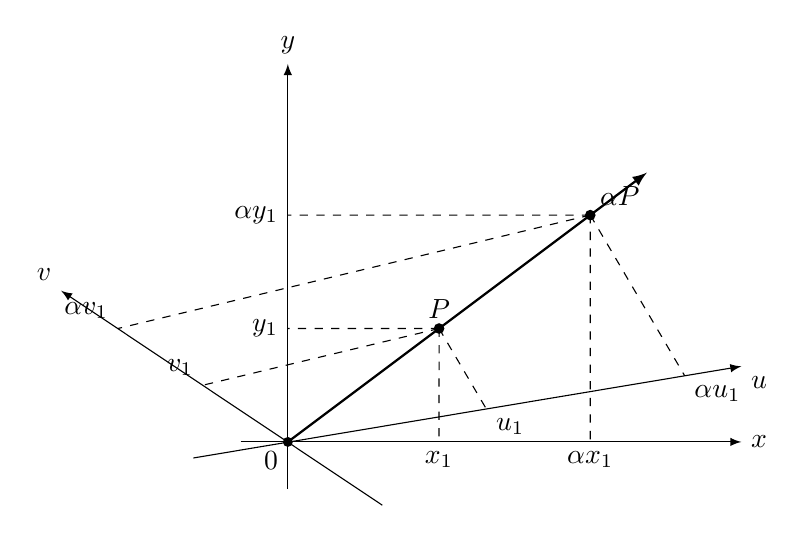
\begin{tikzpicture}[>=latex, scale=1.2]
  \draw[->] (-0.5,0) -- (4.8,0) node[right]{$x$};
  \draw[->] (0,-0.5) -- (0,4.0) node[above]{$y$};
  \fill (0,0) circle (1.5pt) node[below left]{$0$};
  \draw[->] (-1.0,-0.17) -- (4.8,0.8) node[below right]{$u$};
  \draw[->] (1.0,-0.67) -- (-2.4,1.6) node[above left]{$v$};
  \coordinate (P) at (1.6,1.2);
  \coordinate (aP) at (3.2,2.4);
  \fill (P) circle (1.6pt) node[above]{$P$};
  \fill (aP) circle (1.6pt) node[above right]{$\alpha P$};
  \draw[thick, ->] (0,0) -- (3.8,2.85);
  % 投影 P
  \draw[dashed] (P) -- (1.6,0) node[below]{$x_1$};
  \draw[dashed] (P) -- (0,1.2) node[left]{$y_1$};
  \draw[dashed] (P) -- (2.1,0.35) node[below right]{$u_1$};
  \draw[dashed] (P) -- (-0.9,0.6) node[above left]{$v_1$};
  % 投影 \alpha P
  \draw[dashed] (aP) -- (3.2,0) node[below]{$\alpha x_1$};
  \draw[dashed] (aP) -- (0,2.4) node[left]{$\alpha y_1$};
  \draw[dashed] (aP) -- (4.2,0.7) node[below right]{$\alpha u_1$};
  \draw[dashed] (aP) -- (-1.8,1.2) node[above left]{$\alpha v_1$};
\end{tikzpicture}
\end{center}

其中 $\alpha P \in E$ 是由 $P$ 以 $0$ 为中心,以因子 $\alpha$ 伸缩而得到的点.由截线定理(Strahlensatz)随之可知, $\alpha P$ 关于轴 $x, y$ 或 $u, v$ 的坐标同样是从 $P$ 的相应坐标以因子 $\alpha$ 伸缩而得.这意味着
\[
\varphi(\alpha P) = (\alpha x_1, \alpha y_1) = \alpha(x_1, y_1), \qquad \psi(\alpha P) = (\alpha u_1, \alpha v_1) = \alpha(u_1, v_1),
\]
从而
\[
f\big(\alpha(x_1, y_1)\big) = \psi\big(\varphi^{-1}\big(\alpha(x_1, y_1)\big)\big) = \psi(\alpha P) = \alpha(u_1, v_1) = \alpha f\big((x_1, y_1)\big),
\]
即 $f$ 与 $\mathbb{R}^2$ 的数量乘法相容.

为证明 $f$ 与加法的相容性, 我们先考察下面的草图:

\begin{center}
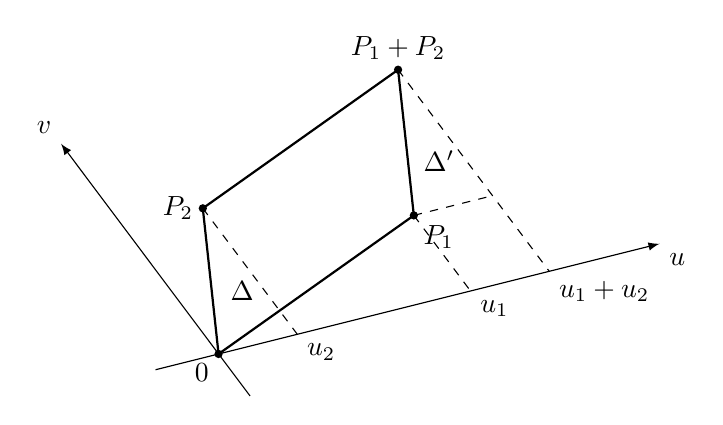
\begin{tikzpicture}[>=latex, scale=1.0]
  % Basis directions
  % u axis
  \draw[->] (-0.8,-0.2) -- (5.6,1.4) node[below right]{$u$};
  % v axis
  \draw[->] (0.4,-0.533) -- (-2.0,2.67) node[above left]{$v$};
  
  \coordinate (O) at (0,0);
  \node[below left] at (O) {$0$};
  
  % Coordinates:
  % u2 = (1.0, 0.25), u1 = (3.2, 0.8), u12 = (4.2, 1.05)
  % P2 = (-0.2, 1.85), P1 = (2.48, 1.76), P12 = (2.28, 3.61)
  % Q = (3.48, 2.01)
  \coordinate (u2) at (1.0, 0.25);
  \coordinate (u1) at (3.2, 0.8);
  \coordinate (u12) at (4.2, 1.05);
  
  \coordinate (P2) at (-0.2, 1.85);
  \coordinate (P1) at (2.48, 1.76);
  \coordinate (P12) at (2.28, 3.61);
  \coordinate (Q) at (3.48, 2.01);
  
  % Parallelogram
  \draw[thick] (O) -- (P1) -- (P12) -- (P2) -- cycle;
  
  % Dashed projection lines
  \draw[dashed] (P2) -- (u2);
  \draw[dashed] (P1) -- (u1);
  \draw[dashed] (P1) -- (Q);
  \draw[dashed] (P12) -- (u12);
  
  % Points
  \fill (O) circle (1.5pt);
  \fill (P1) circle (1.5pt) node[below right]{$P_1$};
  \fill (P2) circle (1.5pt) node[left]{$P_2$};
  \fill (P12) circle (1.5pt) node[above]{$P_1 + P_2$};
  
  % u-axis ticks/labels
  \node[below right] at (u2) {$u_2$};
  \node[below right] at (u1) {$u_1$};
  \node[below right] at (u12) {$u_1 + u_2$};
  
  % Triangles Delta and Delta'
  \node at (0.3, 0.8) {$\Delta$};
  \node at (2.8, 2.45) {$\Delta'$};
\end{tikzpicture}
\end{center}

为清楚起见, 这里我们只限于一个(斜角的)坐标系, 即以 $u$ 和 $v$ 为轴.由点 $P_1, P_2 \in E$ 出发, 点 $P_1 + P_2$ 按通常的平行四边形构造定义.分别包含虚线段的三角形 $\Delta$ 与 $\Delta'$ 可以看作全等, 于是 $P_1 + P_2$ 的 $u$-坐标等于 $P_1$ 与 $P_2$ 的 $u$-坐标之和.对 $v$-坐标以及关于其他坐标系的情形成立相应结论.

现在从两个点 $(x_1, y_1), (x_2, y_2) \in \mathbb{R}^2$ 出发, 考察满足 $\varphi(P_i) = (x_i, y_i)$, $i = 1, 2$, 的对应点 $P_1, P_2 \in E$, 则由上述观察, 结合 $\psi(P_i) = (u_i, v_i)$ 得
\[
\begin{array}{l}
\varphi(P_1 + P_2) = (x_1 + x_2, y_1 + y_2) = (x_1, y_1) + (x_2, y_2), \\
\psi(P_1 + P_2) = (u_1 + u_2, v_1 + v_2) = (u_1, v_1) + (u_2, v_2)\text{.}
\end{array}
\]
$f$ 与 $\mathbb{R}^2$ 上加法的所要求相容性于是由方程
\[
\begin{array}{c}
f\big((x_1, y_1) + (x_2, y_2)\big) = \psi\big(\varphi^{-1}\big((x_1, y_1) + (x_2, y_2)\big)\big) = \psi(P_1 + P_2) \\
= (u_1, v_1) + (u_2, v_2) = f\big((x_1, y_1)\big) + f\big((x_2, y_2)\big)
\end{array}
\]
推出, 于是如所断言, $f \colon \mathbb{R}^2 \longrightarrow \mathbb{R}^2$ 是 $\mathbb{R}$-向量空间的同构.

上述考虑有一个重要结论.若在平面 $E$ 中选一点 $0$ 作为零点, 则 $E$ 可以很自然地配备 $\mathbb{R}$-向量空间结构.即选取 $0$ 处的一个坐标系, 并把相应的双射 $\varphi \colon E \longrightarrow \mathbb{R}^2$(它把点 $P \in E$ 对应于相应的坐标)视为等同.这样由 $\mathbb{R}^2$ 传到 $E$ 上的向量空间结构不依赖于 $E$ 在 $0$ 处坐标系的选择.事实上, 若 $\psi \colon E \longrightarrow \mathbb{R}^2$ 是对应于 $E$ 在 $0$ 处的另一个坐标系的另一个双射, 则我们刚才已经证明复合 $\psi \circ \varphi^{-1} \colon \mathbb{R}^2 \longrightarrow \mathbb{R}^2$ 是同构.这意味着借助 $\varphi$ 由 $\mathbb{R}^2$ 传到 $E$ 上的加法与数量乘法, 分别与借助 $\psi$ 由 $\mathbb{R}^2$ 传到 $E$ 上的加法与数量乘法一致.因此我们完全有理由说, 一个带点的平面, 即一个具有选作零点的点 $0$ 的平面, 自然具有 $\mathbb{R}$-向量空间结构, 而且这个向量空间归根到底无非是众所周知的模型 $\mathbb{R}^2$, 更准确地说, $E$ 作为 $\mathbb{R}$-向量空间同构于 $\mathbb{R}^2$.相应地, 对直线及其模型 $\mathbb{R}^1$, 以及对三维直观空间及其模型 $\mathbb{R}^3$, 也自然有相同的结论.更一般地, 还可以避免模型对零点选取的依赖.此时需要考察所谓的\emph{仿射映射}(\textup{affine Abbildung})\index{fangsheyingshe@仿射映射(affine Abbildung)}, 它们可以表示为线性映射与平移的复合.

同构 $f \colon \mathbb{R}^2 \longrightarrow \mathbb{R}^2$ 的例子有足够多, 例如伸缩
\[
f \colon \mathbb{R}^2 \longrightarrow \mathbb{R}^2, \quad (x_1, y_1) \longmapsto (\alpha_1 x_1, \beta_1 y_1),
\]
其中 $\alpha_1, \beta_1 \in \mathbb{R}^*$ 是预先给定的常数; 又如绕点 $0 \in \mathbb{R}^2$ 转过某个角度 $\vartheta$ 的\emph{旋转}(\textup{Drehung})\index{xuanzhuan@旋转(Drehung)}

\begin{center}
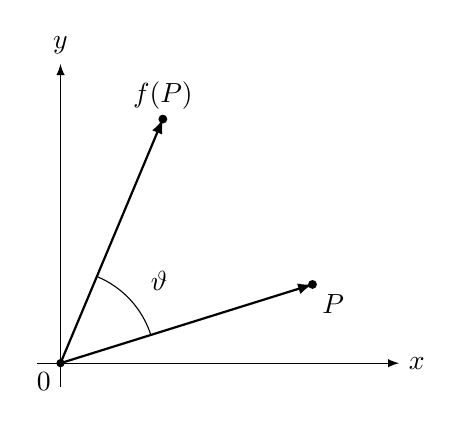
\begin{tikzpicture}[>=latex]
  \draw[->] (-0.3,0) -- (4.3,0) node[right]{$x$};
  \draw[->] (0,-0.3) -- (0,3.8) node[above]{$y$};
  \fill (0,0) circle (1.5pt) node[below left]{$0$};
  \coordinate (P) at (3.2,1.0);
  \coordinate (fP) at (1.3,3.1);
  \fill (P) circle (1.6pt) node[below right]{$P$};
  \fill (fP) circle (1.6pt) node[above]{$f(P)$};
  \draw[thick, ->] (0,0) -- (P);
  \draw[thick, ->] (0,0) -- (fP);
  \draw (1.15,0.35) arc (17.4:67.3:1.2);
  \node at (1.25,1.05) {$\vartheta$};
\end{tikzpicture}
\end{center}

或关于含零点 $0 \in \mathbb{R}^2$ 的直线 $G$ 的\emph{反射}(\textup{Spiegelung})\index{fanshe@反射(Spiegelung)}:

\begin{center}
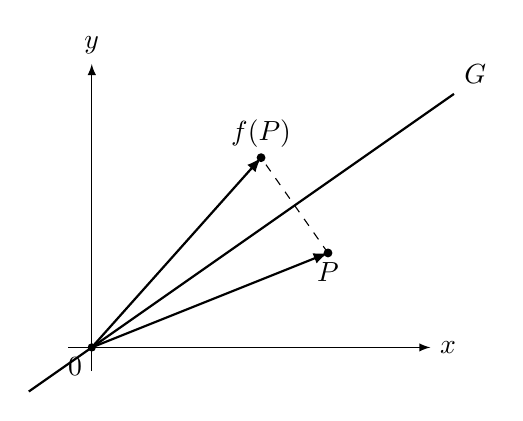
\begin{tikzpicture}[>=latex]
  \draw[->] (-0.3,0) -- (4.3,0) node[right]{$x$};
  \draw[->] (0,-0.3) -- (0,3.6) node[above]{$y$};
  \fill (0,0) circle (1.5pt) node[below left]{$0$};
  \draw[thick] (-0.8,-0.56) -- (4.6,3.22) node[above right]{$G$};
  \coordinate (P) at (3.0,1.2);
  \coordinate (fP) at (2.15,2.41);
  \fill (P) circle (1.6pt) node[below]{$P$};
  \fill (fP) circle (1.6pt) node[above]{$f(P)$};
  \draw[dashed] (P) -- (fP);
  \draw[thick, ->] (0,0) -- (P);
  \draw[thick, ->] (0,0) -- (fP);
\end{tikzpicture}
\end{center}

一个不是双射,因而非同构的线性映射的简单例子是所谓投影
\[
f \colon \mathbb{R}^2 \longrightarrow \mathbb{R}, \qquad (x_1, y_1) \longmapsto x_1\text{.}
\]
这个映射确实可描述为到 $x$-轴的(平行)投影, 做法是把点 $P \in \mathbb{R}^2$ 映到 $x$-轴与过 $P$ 且平行于 $y$-轴的直线的交点:

\begin{center}
\begin{tikzpicture}[>=latex]
  \draw[->] (-0.3,0) -- (4.5,0) node[right]{$x$};
  \draw[->] (0,-0.3) -- (0,3.4) node[above]{$y$};
  \fill (0,0) circle (1.5pt) node[below left]{$0$};
  \coordinate (P) at (3.0,2.0);
  \coordinate (fP) at (3.0,0);
  \fill (P) circle (1.6pt) node[above]{$P$};
  \fill (fP) circle (1.6pt) node[below]{$f(P)$};
  \draw[dashed, thick] (P) -- (fP);
  \draw[thick, ->] (0,0) -- (fP);
\end{tikzpicture}
\end{center}

也可以平行于另一条轴 $v$ 投影, 例如按下面的方式:

\begin{center}
\begin{tikzpicture}[>=latex]
  \draw[->] (-0.4,0) -- (5.2,0) node[right]{$x$};
  \draw[->] (0,-0.3) -- (0,3.0) node[above]{$y$};
  \fill (0,0) circle (1.5pt) node[below left]{$0$};
  \draw[->] (0,0) -- (-2.4,2.0) node[above left]{$v$};
  \coordinate (P) at (2.4,1.8);
  \coordinate (fP) at (4.56,0);
  \fill (P) circle (1.6pt) node[above]{$P$};
  \fill (fP) circle (1.6pt) node[below]{$f(P)$};
  \draw[dashed, thick] (P) -- (fP);
  \draw[thick, ->] (0,0) -- (fP);
\end{tikzpicture}
\end{center}

原则上, 这里得到的并不是本质不同的线性映射, 因为该映射关于坐标轴 $x, v$ 又由
\[
f \colon \mathbb{R}^2 \longrightarrow \mathbb{R}, \qquad (x_1, v_1) \longmapsto x_1
\]
描述.对更高维的向量空间 $\mathbb{R}^n$, 同构或更一般地线性映射的类似例子也可以给出.

在本章中, 我们首先想研究线性映射的一些一般性质, 其中仍考察任意域 $K$ 上的向量空间.例如我们会看到, 满射线性映射 $f \colon V \longrightarrow V'$ 的像 $V'$ 的维数--这里称之为 $f$ 的\emph{秩}(\textup{Rang})\index{zhi@秩(Rang)}--至多等于 $V$ 的维数.因此, 例如满射线性映射 $\mathbb{R}^2 \longrightarrow \mathbb{R}^3$ 的存在性就被排除了.更一般地, 这类现象由线性映射的所谓维数公式支配.还会看到, 线性映射 $f \colon V \longrightarrow V'$ 已经由预先给定的基 $(x_i)_{i \in I}$ 在 $V$ 上的像 $f(x_i) \in V'$ 唯一确定, 甚至只需以(任意方式)给定 $V'$ 中的像 $f(x_i)$, 就可以唯一地定义一个线性映射 $f \colon V \longrightarrow V'$.这个性质对于借助\emph{矩阵}(\textup{Matrix})\index{juzhen@矩阵(Matrix)}(即以基础域 $K$ 的元素为系数的矩形系数表)描述线性映射, 从而对于线性映射的数值处理很重要.不过对矩阵的更深入研究要到第 3 章才进行.

我们要在这个章解决的另一个问题, 涉及构造具有给定\emph{纤维}(\textup{Faser})\index{xianwei@纤维(Faser)} $f^{-1}(f(a)) \subset V$($a$ 在 $V$ 中变化)的线性映射 $f \colon V \longrightarrow V'$.容易看出, 对线性映射 $f \colon V \longrightarrow V'$, 在 $a = 0$ 处的纤维 $f^{-1}(f(0)) = f^{-1}(0)$ 定义一个线性子空间 $U \subset V$, 即 $f$ 的所谓核, 记为 $\ker f$; 而对 $a \in V$ 有
\[
f^{-1}(f(a)) = a + U = \{a + u;\, u \in U\}\text{.}
\]
因此, 把线性子空间 $U = \ker f$ 沿一切向量 $a \in V$ 平行移动, 就得到 $f$ 的纤维; 每个这样的平行移动子空间 $A = a + U$ 都称为 $V$ 的一个属于 $U$ 的\emph{仿射子空间}(\textup{affiner Unterraum})\index{fangshezikongjian@仿射子空间(affiner Unterraum)}.在 $V = \mathbb{R}^2$ 且 $U \subset \mathbb{R}^2$ 是一条直线的情形下, 例如得到下图:

\begin{center}
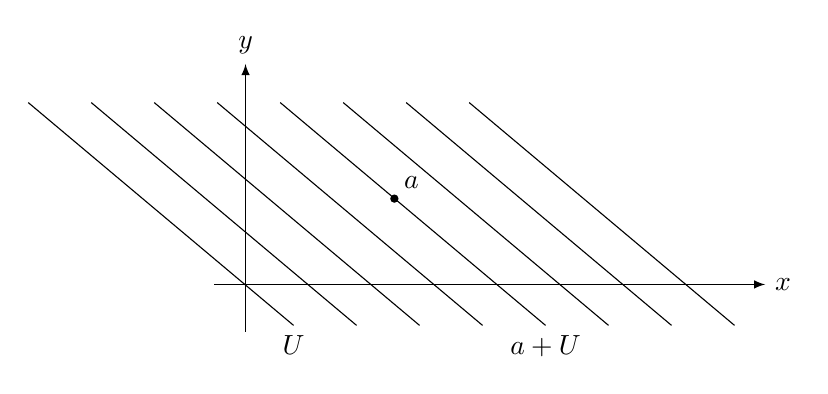
\begin{tikzpicture}[>=latex]
  \draw[->] (-0.4, 0) -- (6.6, 0) node[right]{$x$};
  \draw[->] (0, -0.6) -- (0, 2.8) node[above]{$y$};
  
  \foreach \k in {0,...,7} {
    \draw ({-2.76 + \k*0.80}, 2.31) -- ({0.61 + \k*0.80}, -0.52);
  }
  
  \node[below] at (0.61, -0.52) {$U$};
  \node[below] at ({0.61 + 4*0.80}, -0.52) {$a + U$};
  
  \coordinate (A) at (1.89, 1.09);
  \fill (A) circle (1.5pt);
  \node[above right] at (A) {$a$};
\end{tikzpicture}
\end{center}

反过来, 对线性子空间 $U \subset V$, 我们想考察一切属于 $U$ 的仿射子空间之集 $V/U$, 并把它以自然的方式做成 $K$-向量空间, 办法是对 $a, b \in V$ 与 $\alpha \in K$ 令
\[
(a + U) + (b + U) := (a + b) + U, \qquad \alpha(a + U) := \alpha a + U\text{.}
\]
这样确实得到一个向量空间, 即所谓的\emph{商向量空间}(\textup{Quotientenvektorraum})\index{shangxiangliangkongjian@商向量空间(Quotientenvektorraum)}或\emph{剩余类向量空间}(\textup{Restklassenvektorraum})\index{shengyuleixiangliangkongjian@剩余类向量空间(Restklassenvektorraum)} $V/U$, 这需要一些我们将在下面逐一进行的验证.尤其会看到, 此时\emph{典范映射}(\textup{kanonische Abbildung})\index{dianfanyingshe@典范映射(kanonische Abbildung)}
\[
\pi \colon V \longrightarrow V/U, \quad a \longmapsto a + U
\]
给出一个满足 $\ker \pi = U$ 的线性映射, 其纤维恰好是 $V$ 中属于 $U$ 的仿射子空间.映射 $\pi$ 满足一个重要的,所谓\emph{泛性质}(\textup{universelle Eigenschaft})\index{fanxingzhi@泛性质(universelle Eigenschaft)}: 若 $f \colon V \longrightarrow V'$ 是核满足 $U = \ker \pi \subset \ker f$ 的线性映射, 则 $f$ 分解为复合
\[
f \colon V \xrightarrow{\pi} V/U \xrightarrow{\bar{f}} V'
\]
其中 $\bar{f} \colon V/U \longrightarrow V'$ 是唯一确定的线性映射; 这本质上就是线性映射的\emph{同态定理}(\textup{Homomorphiesatz})\index{tongtaidingli@同态定理(Homomorphiesatz)}的断言.

把向量空间定义为带加法与数量乘法的集合, 并没有对集合元素的种类作任何规定.我们在定义\emph{剩余类}(\textup{Restklasse})\index{shengyulei@剩余类(Restklasse)}向量空间 $V/U$ 时尤其利用了这一点: 它的元素是 $V$ 的仿射子空间, 因而是 $V$ 的子集.可由给定 $K$-向量空间 $V$ 构造的另一个向量空间的例子是\emph{对偶空间}(\textup{Dualraum})\index{duioukongjian@对偶空间(Dualraum)} $V^*$.它的元素是线性映射, 即线性映射 $V \longrightarrow K$.在 $V$ 与 $V^*$ 之间存在着紧密的对称关系; 人们称之为 $V$ 与 $V^*$ 之间的对偶性, 对偶空间因此得名.例如在有限维的情形下, $V$ 本身又可以解释为 $V^*$ 的对偶空间.借助向量空间 $V$ 的对偶空间, 我们在某种意义上从更高层次揭示 $V$ 的线性性质.要证明的结果将在某些情形下使我们能够用概念性的论证代替原本必要的常规计算.


\section{基本概念}\label{sec:2.1}

对 $K$-向量空间 $V$ 的向量 $a_1, \ldots, a_n$, 人们总可以考虑映射
\[
f \colon K^n \longrightarrow V, \quad (\alpha_1, \ldots, \alpha_n) \longmapsto \sum_{i = 1}^{n} \alpha_i a_i\text{.}
\]
对构成 $K^n$ 的标准基的单位向量 $e_i = (\delta_{1i}, \ldots, \delta_{ni}) \in K^n$, $i = 1, \ldots, n$, 有 $f(e_i) = a_i$, 因而我们也可以等价地说, $f$ 由规则
\[
f\left(\sum_{i = 1}^{n} \alpha_i e_i\right) = \sum_{i = 1}^{n} \alpha_i a_i
\]
描述.若 $a_1, \ldots, a_n$ 甚至构成 $V$ 的一个基, 则每个元素 $a \in V$ 都有唯一确定的表示 $a = \sum_{i = 1}^{n} \alpha_i a_i$(系数 $\alpha_i \in K$), 此时可以看出映射 $f$ 是双射.又因为 $f$ 与 $K^n$ 和 $V$ 上的向量空间结构相容--即对 $a, b \in K^n$ 有 $f(a + b) = f(a) + f(b)$, 对 $\alpha \in K$, $a \in K^n$ 有 $f(\alpha a) = \alpha f(a)$--, 所以在选定基 $a_1, \ldots, a_n$ 之后可以借助映射 $f$ 把 $V$ 与 $K^n$ 等同起来.这尤其表明, 尊重向量空间结构的向量空间之间的映射是值得关注的.

\begin{definition}[$K$-线性映射]\label{def:2.1.1}\index{xianxingyingshe@线性映射(lineare Abbildung)}
$K$-向量空间 $V, V'$ 之间的一个映射 $f \colon V \longrightarrow V'$ 称为 $K$-同态或 $K$-线性映射, 如果下列条件成立:
\begin{enumerate}
\item[(i)] $f(a + b) = f(a) + f(b)$ 对 $a, b \in V$;
\item[(ii)] $f(\alpha a) = \alpha f(a)$ 对 $\alpha \in K$, $a \in V$.
\end{enumerate}
\end{definition}

条件 (i) 与 (ii) 可以合并, 即对 $\alpha, \beta \in K$, $a, b \in V$, 可以等价地要求
\[
f(\alpha a + \beta b) = \alpha f(a) + \beta f(b)\text{.}
\]
作为简单的运算规则容易验证:
\[
f(0) = 0, \qquad f(-a) = -f(a) \quad \text{对} \ a \in V\text{.}
\]
此外, 线性映射的复合仍是线性的.下面我们来看几个线性映射的简单例子.

\begin{bsp}\label{bsp:2.1.1}
映射 $\mathbb{C} \longrightarrow \mathbb{C}$, $z \longmapsto \bar{z} = \operatorname{Re}(z) - i\operatorname{Im}(z)$, 是 $\mathbb{R}$-线性的, 但不是 $\mathbb{C}$-线性的.
\end{bsp}

\begin{bsp}\label{bsp:2.1.2}
对 $K$-向量空间 $V$, 恒等映射 $\operatorname{id} \colon V \longrightarrow V$, $a \longmapsto a$, 是 $K$-线性映射的一个例子, 零映射 $0 \colon V \longrightarrow 0$(它把每个元素 $a \in V$ 都映到 $0$)亦然.此外, 对线性子空间 $U \subset V$, 包含映射 $U \hookrightarrow V$ 也是 $K$-线性映射的一个例子.
\end{bsp}

\begin{bsp}\label{bsp:2.1.3}
设 $K$ 是一个域.对 $m, n \in \mathbb{N}$, 考虑 $K$ 中元素构成的一个系统
\[
(\lambda_{ij})_{\substack{i = 1, \ldots, m \\ j = 1, \ldots, n}} = \begin{pmatrix} \lambda_{11} & \cdots & \lambda_{1n} \\ \vdots & & \vdots \\ \lambda_{m1} & \cdots & \lambda_{mn} \end{pmatrix};
\]
人们称它为矩阵.于是由
\[
K^n \longrightarrow K^m, \quad (\alpha_1, \ldots, \alpha_n) \longmapsto \left(\sum_{j = 1}^{n} \lambda_{1j}\alpha_j, \ldots, \sum_{j = 1}^{n} \lambda_{mj}\alpha_j\right)
\]
给出一个 $K$-线性映射.我们后面甚至还会看到, 每个线性映射 $K^n \longrightarrow K^m$ 都具有这种形式, 即可以由一个 $K$ 中元素的矩阵描述.不过那时我们会一贯地把 $K^n$ 或 $K^m$ 中的向量写成列向量, 而不再像迄今那样写成\emph{行向量}(\textup{Zeilen-Vektor})\index{hangxiangliang@行向量(Zeilen-Vektor)}, 因为这样便于随后引入的矩阵乘积.
\end{bsp}

人们把 $K$-向量空间之间的 $K$-线性映射 $f \colon V \longrightarrow V'$ 称为\emph{单同态}(\textup{Monomorphismus})\index{dantongtai@单同态(Monomorphismus)}, 如果 $f$ 是单射的; 称为\emph{满同态}(\textup{Epimorphismus})\index{mantongtai@满同态(Epimorphismus)}, 如果 $f$ 是满射的; 称为同构, 如果 $f$ 是双射的.

\begin{remark}[同构的逆]\label{rem:2.1.2}\index{tonggou@同构(Isomorphismus)}
若 $f \colon V \longrightarrow V'$ 是 $K$-向量空间之间的一个同构, 则存在逆映射 $f^{-1} \colon V' \longrightarrow V$, 并且 $f^{-1}$ 是 $K$-线性的, 因而又是一个同构.
\end{remark}

\begin{proof}
只需证明逆映射 $f^{-1}$ 的 $K$-线性.设 $a', b' \in V'$ 给定.对 $a = f^{-1}(a')$ 与 $b = f^{-1}(b')$ 有 $a' = f(a)$, $b' = f(b)$, 并且由 $f$ 的线性得 $a' + b' = f(a + b)$.于是
\[
f^{-1}(a' + b') = a + b = f^{-1}(a') + f^{-1}(b')\text{.}
\]
对 $\alpha \in K$ 又有 $\alpha a' = f(\alpha a)$, 从而
\[
f^{-1}(\alpha a') = \alpha a = \alpha f^{-1}(a')\text{.}
\]
故 $f^{-1}$ 是 $K$-线性的.
\end{proof}

同构我们常写成 $V \overset{\sim}{\longrightarrow} V'$ 的形式.当 $V = V'$ 时, $K$-线性映射 $f \colon V \longrightarrow V$ 也称为 $V$ 的\emph{自同态}(\textup{Endomorphismus})\index{zitongtai@自同态(Endomorphismus)}, 并把 $V$ 的双射自同态理解为 $V$ 的\emph{自同构}(\textup{Automorphismus})\index{zitonggou@自同构(Automorphismus)}.

\begin{remark}[核与像]\label{rem:2.1.3}\index{he@核(Kern)}\index{xiang@像(Bild)}
设 $f \colon V \longrightarrow V'$ 是向量空间之间的 $K$-线性映射.则
\[
\ker f = f^{-1}(0) = \{a \in V;\, f(a) = 0\} \qquad \text{与} \qquad \operatorname{im} f = f(V) = \{f(a);\, a \in V\}
\]
分别是 $V$ 与 $V'$ 的线性子空间; 它们称为 $f$ 的核与像.
\end{remark}

证明很简单.对 $a, b \in \ker f$ 有
\[
f(a + b) = f(a) + f(b) = 0 + 0 = 0,
\]
即 $a + b \in \ker f$.又有 $f(\alpha a) = \alpha f(a) = \alpha 0 = 0$, 从而对 $\alpha \in K$, $a \in \ker f$ 有 $\alpha a \in \ker f$.由于 $0 \in \ker f$, 核 $\ker f \neq \emptyset$, 故 $\ker f$ 是 $V$ 的线性子空间.

类似地可以看出 $\operatorname{im} f$ 是 $V'$ 的线性子空间.因 $0 \in \operatorname{im} f$, $\operatorname{im} f$ 至少非空.再设 $\alpha \in K$, $a', b' \in \operatorname{im} f$, 例如 $a' = f(a)$, $b' = f(b)$($a, b \in V$).则 $\alpha a' = f(\alpha a)$, 且 $a' + b' = f(a + b)$, 即 $\alpha a', a' + b' \in \operatorname{im} f$.所以 $\operatorname{im} f$ 也是 $V'$ 的线性子空间.

\begin{remark}[单射的刻画]\label{rem:2.1.4}
向量空间之间的 $K$-线性映射 $f \colon V \longrightarrow V'$ 是单射的, 当且仅当 $\ker f = 0$.
\end{remark}

\begin{proof}
先设 $f$ 是单射.则 $\ker f = f^{-1}(0)$ 尤其至多含一个元素, 又因 $0 \in f^{-1}(0)$, 得 $\ker f = 0$.再反过来设 $\ker f = 0$ 成立, 设 $a, b \in V$ 满足 $f(a) = f(b)$.于是
\[
f(a - b) = f(a) - f(b) = 0,
\]
即 $a - b \in \ker f = 0$, 从而 $a = b$, 也就是说 $f$ 是单射.
\end{proof}

我们继续考察生成系以及线性相关或线性无关组在应用线性映射时的行为.

\begin{remark}\label{rem:2.1.5}
设 $f \colon V \longrightarrow V'$ 是向量空间之间的 $K$-线性映射.
\begin{enumerate}
\item[(i)] 对子集 $A \subset V$ 有 $f(\langle A \rangle) = \langle f(A) \rangle$.
\item[(ii)] 设向量 $a_1, \ldots, a_n \in V$ 线性相关.则其像 $f(a_1), \ldots, f(a_n) \in V'$ 也线性相关.当 $f$ 是单射时, 逆命题成立.
\item[(iii)] 设向量 $a_1, \ldots, a_n \in V$ 的像 $f(a_1), \ldots, f(a_n) \in V'$ 线性无关.则 $a_1, \ldots, a_n$ 也线性无关.当 $f$ 是单射时, 逆命题成立.
\end{enumerate}
\end{remark}

证明可以通过简单验证定义来完成.相应的计算留给读者.作为断言 (iii) 的推论我们还记下:

\begin{remark}\label{rem:2.1.6}
对向量空间之间的 $K$-线性映射 $f \colon V \longrightarrow V'$ 有 $\dim f(V) \leq \dim_K V$.
\end{remark}

线性映射的一个重要性质在于, 它们已经由在定义域空间的一个基上取的值唯一确定.

\begin{theorem}[线性映射的确定]\label{thm:2.1.7}
设 $V$ 是带生成系 $a_1, \ldots, a_n$ 的 $K$-向量空间.若 $a_1', \ldots, a_n'$ 是另一个 $K$-向量空间 $V'$ 的任意向量, 则:
\begin{enumerate}
\item[(i)] 至多存在一个满足 $f(a_i) = a_i'$($i = 1, \ldots, n$)的 $K$-线性映射 $f \colon V \longrightarrow V'$;
\item[(ii)] 若 $a_1, \ldots, a_n$ 甚至是 $V$ 的一个基, 则恰存在一个满足 $f(a_i) = a_i'$($i = 1, \ldots, n$)的 $K$-线性映射 $f \colon V \longrightarrow V'$.
\end{enumerate}
\end{theorem}

\begin{proof}
我们从唯一性断言 (i) 开始.设 $f \colon V \longrightarrow V'$ 是 $K$-线性的, 满足 $f(a_i) = a_i'$, $i = 1, \ldots, n$, 并设 $a \in V$.则 $a$ 有形如 $a = \sum_{i = 1}^{n} \alpha_i a_i$ 的表示(系数 $\alpha_i \in K$).由 $f$ 的线性得
\[
f(a) = f\left(\sum_{i = 1}^{n} \alpha_i a_i\right) = \sum_{i = 1}^{n} \alpha_i f(a_i),
\]
这意味着 $f(a)$ 由值 $f(a_i)$, $i = 1, \ldots, n$, 唯一确定.

在情形 (ii) 中, 若 $a_1, \ldots, a_n$ 构成 $V$ 的一个基, 则对 $a \in V$, 表示 $a = \sum_{i = 1}^{n} \alpha_i a_i$ 中的系数 $\alpha_i$ 唯一确定, 因而可以按
\[
f(a) = \sum_{i = 1}^{n} \alpha_i f(a_i)
\]
定义一个映射 $f \colon V \longrightarrow V'$.这个映射是 $K$-线性的.事实上, 若 $a = \sum_{i = 1}^{n} \alpha_i a_i$ 与 $b = \sum_{i = 1}^{n} \beta_i a_i$ 是 $V$ 的两个元素, 则
\[
a + b = \sum_{i = 1}^{n} (\alpha_i + \beta_i) a_i\text{.}
\]
由于这是 $a + b$ 作为 $a_1, \ldots, a_n$ 的线性组合的(唯一确定的)表示, 得
\[
f(a + b) = \sum_{i = 1}^{n} (\alpha_i + \beta_i) a_i' = \sum_{i = 1}^{n} \alpha_i a_i' + \sum_{i = 1}^{n} \beta_i a_i' = f(a) + f(b)\text{.}
\]
相应地, 对 $\alpha \in K$ 计算得
\[
f(\alpha a) = f\left(\sum_{i = 1}^{n} \alpha\alpha_i a_i\right) = \sum_{i = 1}^{n} \alpha\alpha_i a_i' = \alpha \sum_{i = 1}^{n} \alpha_i a_i' = \alpha f(a),
\]
由此可见 $f \colon V \longrightarrow V'$ 是 $K$-线性的.故存在满足 $f(a_i) = a_i'$ 的 $K$-线性映射 $f \colon V \longrightarrow V'$, 并且如 (i) 中所见, 它是唯一确定的.
\end{proof}

对两个 $K$-向量空间 $V$ 和 $V'$, 一切 $K$-线性映射 $f \colon V \longrightarrow V'$ 构成一个 $K$-向量空间, 可以说是 $V$ 上一切 $K$-线性 $V'$ 值函数的向量空间; 它通常记为 $\operatorname{Hom}_K(V, V')$, 即
\[
\operatorname{Hom}_K(V, V') = \{f \colon V \longrightarrow V';\, f\ \text{$K$-线性}\}\text{.}
\]
其中对 $f, g \in \operatorname{Hom}_K(V, V')$, 和 $f + g$ 由
\[
f + g \colon V \longrightarrow V', \quad x \longmapsto f(x) + g(x)
\]
定义; 相应地, 对 $\alpha \in K$, 乘积 $\alpha \cdot f$ 由
\[
\alpha \cdot f \colon V \longrightarrow V', \quad x \longmapsto \alpha \cdot (f(x))
\]
定义.通过简单计算即可验证, $f + g$ 与 $\alpha \cdot f$ 又是从 $V$ 到 $V'$ 的 $K$-线性映射.定理~\mtref{thm:2.1.7} 断言 (ii) 的情形于是可以更精确地表述为: 对 $V$ 的一个基 $a_1, \ldots, a_n$, 对应 $f \longmapsto (f(a_1), \ldots, f(a_n))$ 给出 $K$-向量空间的同构
\[
\operatorname{Hom}_K(V, V') \overset{\sim}{\longrightarrow} (V')^n\text{.}
\]

如果我们除了 $V$ 的基 $a_1, \ldots, a_n$ 之外还在 $V'$ 中固定一个基, 那么上述对应可以描述得更加具体.设 $b_1, \ldots, b_m$ 是 $V'$ 的一个基, 其中假定 $V'$ 有限维.则每个向量 $a' \in V'$ 都有唯一表示 $a' = \sum_{i = 1}^{m} \lambda_i b_i$, 因而由系数元组 $(\lambda_1, \ldots, \lambda_m)$ 以一一对应方式唯一确定.线性映射 $f \colon V \longrightarrow V'$ 因此对应于 $n$ 个这样的系数元组 $(\lambda_{1j}, \ldots, \lambda_{mj})$, $j = 1, \ldots, n$, 我们把这些元组解释为列并拼成一个矩阵:
\[
(\lambda_{ij})_{\substack{i = 1, \ldots, m \\ j = 1, \ldots, n}} = \begin{pmatrix} \lambda_{11} & \cdots & \lambda_{1n} \\ \vdots & & \vdots \\ \lambda_{m1} & \cdots & \lambda_{mn} \end{pmatrix}\text{.}
\]
人们称它为属于线性映射 $f$ 的矩阵, 其中这一称呼自然是相对于 $V$ 与 $V'$ 中固定的基而言的.线性映射 $f$ 可以借助矩阵 $(\lambda_{ij})$ 通过方程
\[
f(a_j) = \sum_{i = 1}^{m} \lambda_{ij} b_i, \quad j = 1, \ldots, n,
\]
即通过
\[
f\left(\sum_{j = 1}^{n} \alpha_j a_j\right) = \sum_{i = 1}^{m} \left(\sum_{j = 1}^{n} \lambda_{ij}\alpha_j\right) b_i
\]
重建出来.

\begin{theorem}\label{thm:2.1.8}
设 $V, V'$ 是 $K$-向量空间.
\begin{enumerate}
\item[(i)] 若存在同构 $f \colon V \longrightarrow V'$, 则 $V$ 与 $V'$ 的维数一致, 即 $\dim_K V = \dim_K V'$.
\item[(ii)] 反过来, 当 $\dim_K V = \dim_K V' < \infty$ 时, 总存在同构 $f \colon V \longrightarrow V'$.
\end{enumerate}
\end{theorem}

\begin{proof}
若 $f \colon V \longrightarrow V'$ 是同构, 则由注记~\mtref{rem:2.1.5} 可见, 向量组 $a_1, \ldots, a_n \in V$ 线性无关, 当且仅当其像 $f(a_1), \ldots, f(a_n) \in V'$ 线性无关.这意味着 $\dim_K V = \dim_K V'$.

反过来, 若 $\dim_K V = \dim_K V' = n < \infty$, 则选取两个基 $a_1, \ldots, a_n \in V$ 与 $a_1', \ldots, a_n' \in V'$.按定理~\mtref{thm:2.1.7} (ii), 存在唯一确定的 $K$-线性映射 $f \colon V \longrightarrow V'$, 满足 $f(a_i) = a_i'$, $i = 1, \ldots, n$.若 $a \in \ker f$, 例如 $a = \sum_{i = 1}^{n} \alpha_i a_i$(系数 $\alpha_i \in K$), 则 $\sum_{i = 1}^{n} \alpha_i a_i' = f(a) = 0$, 由 $a_1', \ldots, a_n'$ 的线性无关性已有 $\alpha_i = 0$ 对一切 $i$, 从而 $a = 0$.故 $f$ 是单射.但 $f$ 也是满射: 元素 $a' \in V'$ 总可以写成 $a' = \sum_{i = 1}^{n} \alpha_i a_i'$(系数 $\alpha_i \in K$), 且有 $f\left(\sum_{i = 1}^{n} \alpha_i a_i\right) = a'$.
\end{proof}

\begin{corollary}\label{cor:2.1.9}
若 $V$ 是维数 $n < \infty$ 的 $K$-向量空间, 则存在同构 $V \overset{\sim}{\longrightarrow} K^n$.
\end{corollary}

这意味着, 除去同构之外, 有限维 $K$-向量空间只有 $K^n$.我们最后还想证明 $K$-线性映射的所谓维数公式.

\begin{theorem}[维数公式]\label{thm:2.1.10}\index{weishugongshi@维数公式(Dimensionsformel)}\index{zhi@秩(Rang)}
设 $f \colon V \longrightarrow V'$ 是向量空间之间的 $K$-线性映射.则
\[
\dim_K V = \dim_K(\ker f) + \dim_K(\operatorname{im} f)\text{.}
\]
\end{theorem}

不用 $\dim_K(\operatorname{im} f)$, 即像空间 $f(V)$ 的维数, 人们也常写 $\operatorname{rg} f$, 并称之为 $f$ 的秩.

\begin{proof}[定理~\mtref{thm:2.1.10} 的证明]
若 $\ker f$ 与 $\operatorname{im} f$ 之一无穷维, 则 $V$ 也无穷维; 若 $\dim_K(\operatorname{im} f) = \infty$, 则由注记~\mtref{rem:2.1.5} 已得此结论.因此可以把 $\ker f$ 与 $\operatorname{im} f$ 视为有限维.此时在 $V$ 中选取向量 $a_1, \ldots, a_m$, 使其像 $f(a_1), \ldots, f(a_m)$ 构成 $\operatorname{im} f$ 的一个基.再选取 $\ker f$ 的一个基 $a_{m+1}, \ldots, a_n$.只需证明 $a_1, \ldots, a_n$ 构成 $V$ 的一个基.为此考虑向量 $a \in V$.由于 $f(a_1), \ldots, f(a_m)$ 生成 $\operatorname{im} f$, 存在表示 $f(a) = \sum_{i = 1}^{m} \alpha_i f(a_i)$(系数 $\alpha_i \in K$).又向量 $a - \sum_{i = 1}^{m} \alpha_i a_i$ 位于 $f$ 的核中, 而核由 $a_{m+1}, \ldots, a_n$ 生成, 故存在 $\alpha_{m+1}, \ldots, \alpha_n \in K$ 使得
\[
a - \sum_{i = 1}^{m} \alpha_i a_i = \sum_{i = m+1}^{n} \alpha_i a_i,
\]
即 $a = \sum_{i = 1}^{n} \alpha_i a_i$.这表明 $a_1, \ldots, a_n$ 构成 $V$ 的一个生成系.

为看出 $a_1, \ldots, a_n$ 也线性无关, 考虑带系数 $\alpha_i \in K$ 的关系 $\sum_{i = 1}^{n} \alpha_i a_i = 0$.由此得
\[
0 = f\left(\sum_{i = 1}^{n} \alpha_i a_i\right) = \sum_{i = 1}^{n} \alpha_i f(a_i) = \sum_{i = 1}^{m} \alpha_i f(a_i),
\]
由 $f(a_1), \ldots, f(a_m)$ 的线性无关性得 $\alpha_1 = \cdots = \alpha_m = 0$.于是又有 $\sum_{i = m+1}^{n} \alpha_i a_i = 0$, 由 $a_{m+1}, \ldots, a_n$ 的线性无关性继续得 $\alpha_{m+1} = \cdots = \alpha_n = 0$.故系数 $\alpha_1, \ldots, \alpha_n$ 全部消失, 我们看出 $a_1, \ldots, a_n$ 线性无关.
\end{proof}

\begin{corollary}\label{cor:2.1.11}
设 $f \colon V \longrightarrow V'$ 是向量空间之间的 $K$-线性映射, 且 $\dim_K V = \dim_K V' < \infty$.则下列条件等价:
\begin{enumerate}
\item[(i)] $f$ 是单同态;
\item[(ii)] $f$ 是满同态;
\item[(iii)] $f$ 是同构.
\end{enumerate}
\end{corollary}

\begin{proof}
先设条件 (i) 成立, 即 $f$ 是单同态.则利用定理~\mtref{thm:2.1.10} 得
\[
\dim_K V' = \dim_K V = \dim_K(\ker f) + \dim_K(\operatorname{im} f)\text{.}
\]
因 $\dim_K(\ker f) = 0$, 线性子空间 $\operatorname{im} f \subset V'$ 与 $V'$ 具有相同的(有限)维数.由推论~\mtref{cor:1.5.14} (ii) 得 $\operatorname{im} f = V'$, 即 $f$ 是满同态, 条件 (ii) 成立.

再设 $f$ 是满足条件 (ii) 的满同态.维数公式(定理~\mtref{thm:2.1.10})由 $\operatorname{im} f = V'$ 与 $\dim_K V' = \dim_K V$ 推出必有 $\ker f = 0$, 即 $f$ 是单射, 从而满足条件 (iii).最后, (iii) 蕴含条件 (i) 是显然的.
\end{proof}

这里也要指出, 推论~\mtref{cor:2.1.11} 与推论~\mtref{cor:1.5.14} (ii) 类似, 不能推广到无穷维向量空间的情形, 因为无穷维 $K$-向量空间总有真线性子空间具有无穷维.

\aufgaben

\noindent\textbf{习题 1.} 对一个域 $K$ 和 $n \in \mathbb{N}$, 把 $K^n$ 视为 $K$-向量空间.对 $i = 1, \ldots, n$, 设 $p_i \colon K^n \longrightarrow K$ 分别是在第 $i$ 个分量上的投影.证明:
\begin{enumerate}
\item[(i)] 映射 $p_i$ 是 $K$-线性的.
\item[(ii)] 从一个 $K$-向量空间 $V$ 到 $K^n$ 的映射 $f \colon V \longrightarrow K^n$ 是 $K$-线性的, 当且仅当所有复合 $p_i \circ f$ 都是 $K$-线性的.
\end{enumerate}

\noindent\textbf{习题 2.} 是否存在 $\mathbb{R}$-线性映射 $\mathbb{R}^4 \longrightarrow \mathbb{R}^3$, 把下列向量 $a_i \in \mathbb{R}^4$ 分别映到所给向量 $b_i \in \mathbb{R}^3$?(AT 303)
\begin{enumerate}
\item[(i)] $a_1 = (1, 1, 0, 0)$, $a_2 = (1, 1, 1, 0)$, $a_3 = (0, 1, 1, 1)$, $a_4 = (0, 0, 1, 1)$;
$b_1 = (1, 2, 3)$, $b_2 = (2, 3, 1)$, $b_3 = (3, 1, 2)$, $b_4 = (2, 0, 4)$;
\item[(ii)] $a_1 = (0, 1, 1, 1)$, $a_2 = (1, 0, 1, 1)$, $a_3 = (1, 1, 0, 1)$, $a_4 = (-1, 1, 0, 0)$;$b_1, \ldots, b_4$ 同 (i);
\item[(iii)] $a_1 = (0, 1, 1, 1)$, $a_2 = (1, 0, 1, 1)$, $a_3 = (1, 1, 0, 1)$, $a_4 = (0, 2, 0, 1)$;$b_1, \ldots, b_4$ 同 (i).
\end{enumerate}

\noindent\textbf{习题 3.} 确定所有 $\mathbb{R}$-线性映射 $\mathbb{R} \longrightarrow \mathbb{R}$.

\noindent\textbf{习题 4.} 确定所有域同态 $f \colon \mathbb{Q}(\sqrt{2}) \longrightarrow \mathbb{Q}(\sqrt{2})$, 即所有还满足 $f(\alpha\beta) = f(\alpha)f(\beta)$ 的 $\mathbb{Q}$-线性映射.

\noindent\textbf{习题 5.} 设 $V$ 是一个 $K$-向量空间, $f \colon V \longrightarrow V$ 是满足 $f^2 = f$ 的自同态.证明 $V = \ker f \oplus \operatorname{im} f$.(AT 306)

\noindent\textbf{习题 6.} 对 $K$-向量空间 $V$ 的线性子空间 $U, U'$, 考虑映射
\[
\varphi \colon U \times U' \longrightarrow V, \quad (a, b) \longmapsto a - b\text{.}
\]
\begin{enumerate}
\item[(i)] 证明: 如果把 $U \times U'$ 连同逐分量加法与数量乘法视为 $K$-向量空间, 则 $\varphi$ 是 $K$-线性的.
\item[(ii)] 计算 $\dim_K(U \times U')$.
\item[(iii)] 把线性映射的维数公式应用于 $\varphi$, 并由此推出 $V$ 的线性子空间的维数公式
\[
\dim_K U + \dim_K U' = \dim_K(U + U') + \dim_K(U \cap U')\text{.}
\]
\end{enumerate}

\noindent\textbf{习题 7.} 对 $K$-向量空间 $V, V'$, 确定 $\dim_K \operatorname{Hom}_K(V, V')$, 即从 $V$ 到 $V'$ 的一切 $K$-线性映射构成的向量空间的维数.

\noindent\textbf{习题 8.} 设 $V_1 \xrightarrow{f} V_2 \xrightarrow{g} V_3$ 是有限维 $K$-向量空间之间的 $K$-线性映射.证明 (AT 307):
\[
\operatorname{rg} f + \operatorname{rg} g \leq \operatorname{rg}(g \circ f) + \dim_K V_2\text{.}
\]


\section{商向量空间}\label{sec:2.2}

除了向量空间 $V$ 的线性子空间, 即定义~\mtref{def:1.4.2} 意义下的子向量空间之外, 我们还想在本节考察 $V$ 的所谓仿射子空间.它们本质上是由线性子空间沿向量 $a \in V$ 平移(或平行移动)而得到的.

\begin{definition}[仿射子空间]\label{def:2.2.1}\index{fangshezikongjian@仿射子空间(affiner Unterraum)}
设 $V$ 是一个 $K$-向量空间, $A \subset V$ 是一个子集.如果 $A$ 是空的, 或者存在元素 $a \in V$ 与线性子空间 $U \subset V$, 使得
\[
A = a + U := \{a + u;\, u \in U\},
\]
则称 $A$ 为 $V$ 的仿射子空间.
\end{definition}

在定义的情形中, 对 $a \notin U$ 尤其有 $0 \notin a + U$, 由此可知此时 $A = a + U$ 不可能是 $V$ 的线性子空间.本节的目的是证明: 一切形如 $a + U$($a \in V$)的仿射子空间之集可以在自然的方式下成为 $K$-向量空间.我们把这个向量空间记为 $V/U$(读作 $V$ 模 $U$), 并证明对应 $a \longmapsto a + U$ 定义了一个以 $U$ 为核的满射 $K$-线性映射 $V \longrightarrow V/U$.

为了进一步阐明这个问题, 我们首先假定存在满足 $\ker f = U$ 的满射 $K$-线性映射 $f \colon V \longrightarrow V'$.对 $a' \in V'$, 称 $f^{-1}(a')$ 为 $f$ 在 $a'$ 处的纤维.

\begin{remark}\label{rem:2.2.2}
设 $f \colon V \longrightarrow V'$ 是向量空间之间的 $K$-线性映射, 且 $\ker f = U$.则对 $a \in V$, $f$ 在 $f(a)$ 处的纤维恰为仿射子空间 $a + U$, 即 $f^{-1}(f(a)) = a + U$.
\end{remark}

\begin{proof}
对 $u \in U$ 有 $f(a + u) = f(a)$, 因而 $a + U \subset f^{-1}(f(a))$.反过来, 由 $a' \in f^{-1}(f(a))$ 得 $f(a') = f(a)$, 即 $f(a' - a) = 0$.这蕴含 $a' - a \in \ker f = U$, 即 $a' \in a + U$, 从而 $f^{-1}(f(a)) \subset a + U$, 两个集合相等.
\end{proof}

于是我们可以记下: 核为 $U$ 的满射 $K$-线性映射 $f \colon V \longrightarrow V'$ 的纤维恰好是仿射子空间 $a + U$($a \in V$).由于在 $f(V) = V'$ 的每个 $a'$ 上方恰好有一个纤维, 即 $f^{-1}(a')$, 我们可以把 $V$ 中形如 $a + U \subset V$ 的仿射子空间之集与 $V'$ 等同, 并通过承接 $V'$ 的向量空间结构把它做成 $K$-向量空间 $V/U$.于是两个纤维 $f^{-1}(f(a)) = a + U$ 与 $f^{-1}(f(b)) = b + U$ 相加, 就是取 $f(a) + f(b) = f(a + b)$ 上方的纤维, 即
\[
(a + U) + (b + U) = (a + b) + U\text{.}
\]
相应地, 一个纤维 $f^{-1}(f(a)) = a + U$ 与纯量 $\alpha \in K$ 相乘, 就是取 $\alpha f(a) = f(\alpha a)$ 上方的纤维, 即 $\alpha(a + U) = \alpha a + U$.

最后显然, 映射 $V \longrightarrow V/U$, $a \longmapsto a + U$, 与 $f \colon V \longrightarrow V'$ 一样, 是以 $U$ 为核的满射 $K$-线性映射.

上述考虑表明, 把 $V$ 中形如 $a + U \subset V$ 的仿射子空间之集做成 $K$-向量空间的问题, 在拥有满足 $\ker f = U$ 的满射线性映射 $f \colon V \longrightarrow V'$ 时有自然的解.但这样的映射很容易构造.按定理~\mtref{thm:1.6.4} 选取 $U$ 的一个补空间 $U'$, 即满足 $V = U \oplus U'$ 的线性子空间 $U' \subset V$.则每个 $a \in V$ 都能唯一地写成 $a = u + u'$($u \in U$, $u' \in U'$).把 $a$ 对应于和项 $u'$, 我们如愿得到一个以 $U$ 为核的满射 $K$-线性映射 $p \colon V \longrightarrow U'$.称 $p$ 为 $U \oplus U'$ 到第二个和项的投影.

不过在下面的讨论中, 我们要用另一种方式构造商向量空间 $V/U$.所用方法的优点是它不依赖向量空间的特殊性质(线性子空间存在补空间), 而是还能应用于其他场合.

\begin{definition}[\emph{等价关系}\index{dengjiaguanxi@等价关系(Äquivalenzrelation)}]\label{def:2.2.3}\index{dengjiaguanxi@等价关系(Äquivalenzrelation)}
集合 $M$ 上的一个关系由 $M \times M$ 的一个子集 $R$ 构成; 对 $(a, b) \in R$ 记 $a \sim b$, 并称之为关系"$\sim$".$M$ 上的一个关系"$\sim$"称为等价关系, 如果它具有下列性质:
\begin{enumerate}
\item[(i)] \emph{自反性}(\textup{Reflexivität})\index{zifanxing@自反性(Reflexivität)}: 对一切 $a \in M$ 有 $a \sim a$;
\item[(ii)] \emph{对称性}(\textup{Symmetrie})\index{duichenxing@对称性(Symmetrie)}: $a \sim b \Longrightarrow b \sim a$;
\item[(iii)] \emph{传递性}(\textup{Transitivität})\index{chuandixing@传递性(Transitivität)}: $a \sim b$, $b \sim c \Longrightarrow a \sim c$.
\end{enumerate}
\end{definition}

若"$\sim$"是集合 $M$ 上的一个等价关系, 则称满足 $a \sim b$ 的两个元素 $a, b \in M$ 等价.进一步把
\[
[a] = \{b \in M;\, b \sim a\}
\]
称为元素 $a$ 在 $M$ 中的\emph{等价类}(\textup{Äquivalenzklasse})\index{dengjialei@等价类(Äquivalenzklasse)}.为给一个简单例子, 考虑向量空间之间的 $K$-线性映射 $f \colon V \longrightarrow V'$, 并对 $a, b \in V$ 令
\[
a \sim b :\Longleftrightarrow f(a) = f(b)\text{.}
\]
显然, $f$ 借此在 $V$ 上诱导一个等价关系, 且 $[a] = f^{-1}(f(a))$ 是元素 $a \in V$ 的等价类.

在集合 $M$ 上的等价关系"$\sim$"的情形中, 等价类 $[a]$ 的每个元素 $b$ 都称为该类的一个\emph{代表元}(\textup{Repräsentant})\index{daibiaoyuan@代表元(Repräsentant)}.由定义~\mtref{def:2.2.3} (i), 元素 $a \in M$ 恒是类 $[a]$ 的代表元, 因此等价类恒非空.我们想证明: 两个元素 $a, b \in M$ 恰在 $a, b$ 相互等价时诱导出同一个等价类, 即 $[a] = [b]$; 或者说, 它们都等价于某个第三元素 $c \in M$.这尤其蕴含, $M$ 上的等价关系把 $M$ 划分为互不相交的等价类.

\begin{theorem}\label{thm:2.2.4}
设"$\sim$"是集合 $M$ 上的一个等价关系.对元素 $a, b \in M$, 下列条件等价:
\begin{enumerate}
\item[(i)] $a \sim b$;
\item[(ii)] $[a] = [b]$;
\item[(iii)] $[a] \cap [b] \neq \emptyset$.
\end{enumerate}
特别地, $M$ 是与"$\sim$"相联系的等价类的不交并.
\end{theorem}

\begin{proof}
先设 (i) 成立, 即 $a \sim b$.对满足 $c \sim a$ 的 $c \in M$, 由 $a \sim b$ 已有 $c \sim b$, 故 $[a] \subset [b]$.反向包含可以相应验证, 从而整体上得到 (ii) 中的等式 $[a] = [b]$.由于等价类恒非空, (iii) 又是 (ii) 的推论.最后设条件 (iii) 成立, 取元素 $c \in [a] \cap [b]$.则 $c \sim a$, 由对称性即 $a \sim c$, 又有 $c \sim b$, 从而由传递性得 $a \sim b$, 即 (i).
\end{proof}

现在把 $M / \sim$ 定义为 $M$ 中等价类之集, 于是可以考虑典范映射
\[
M \longrightarrow M / \sim, \qquad a \longmapsto [a],
\]
它把元素 $a \in M$ 映到相应的等价类 $[a] \subset M$.由定理~\mtref{thm:2.2.4}, $[a]$ 是 $M$ 中含 $a$ 的唯一确定的等价类.下面我们要研究向量空间上的等价关系.

\begin{remark}[模 $U$ 的\emph{同余}\index{tongyu@同余(Kongruenz)}]\label{rem:2.2.5}\index{shengyulei@剩余类(Restklasse)}
设 $V$ 是一个 $K$-向量空间, $U \subset V$ 是一个线性子空间.则通过
\[
a \sim b :\Longleftrightarrow a - b \in U
\]
在 $V$ 上定义一个等价关系, 也称为模 $U$ 的同余.对元素 $a \in V$ 的等价类 $[a]$ 有 $[a] = a + U$.两个等价类 $[a] = a + U$ 与 $[b] = b + U$ 恰在 $a \sim b$, 即 $a - b \in U$ 时一致.
\end{remark}

\begin{proof}
对一切 $a \in V$ 有 $a - a = 0 \in U$, 故 $a \sim a$, 关系是自反的.其次证明对称性.设 $a \sim b$, 即 $a - b \in U$.则 $b - a = -(a - b) \in U$, 即 $b \sim a$.最后验证传递性.设 $a \sim b$ 与 $b \sim c$, 即 $a - b, b - c \in U$.则
\[
a - c = (a - b) + (b - c) \in U,
\]
即 $a \sim c$.

此外, 向量 $a \in V$ 的等价类计算为
\[
[a] = \{b \in V;\, b \sim a\} = \{b \in V;\, b - a \in U\} = a + U,
\]
正如所断言.最后, 按注记~\mtref{rem:2.2.5}, 两个等价类 $[a]$ 与 $[b]$ 恰在 $a \sim b$, 即 $a - b \in U$ 时一致.
\end{proof}

对 $a \in V$, 把等价类 $[a] = a + U$ 更精确地称为 $a$ 模 $U$ 的剩余类, 或 $a$ 关于 $U$ 的\emph{陪集}(\textup{Nebenklasse})\index{peiji@陪集(Nebenklasse)}.为定义商向量空间 $V/U$, 我们要在这个剩余类之集上定义 $K$-向量空间结构.为此先推导一些剩余类运算的规则, 其中为清楚起见把剩余类 $a + U$ 重新写成等价类 $[a]$ 的形式.

\begin{remark}\label{rem:2.2.6}
在 $K$-向量空间 $V$ 上考虑属于线性子空间 $U \subset V$ 的模 $U$ 同余的等价关系.设对向量 $a, a', b, b' \in V$ 有 $[a] = [a']$ 与 $[b] = [b']$.则 $[a + b] = [a' + b']$, 且对 $\alpha \in K$ 有 $[\alpha a] = [\alpha a']$.
\end{remark}

\begin{proof}
由 $[a] = [a']$, $[b] = [b']$ 得 $a - a', b - b' \in U$, 从而 $(a + b) - (a' + b') = (a - a') + (b - b') \in U$, 即 $[a + b] = [a' + b']$.又有 $\alpha a - \alpha a' = \alpha(a - a') \in U$, 即 $[\alpha a] = [\alpha a']$.
\end{proof}

向量 $a \in V$ 的等价类 $[a]$ 的取法因此与 $V$ 的向量空间结构相容.若用 $V/U$ 表示等价类 $[a] = a + U$($a$ 在 $V$ 中变化)之集, 则可以利用注记~\mtref{rem:2.2.6} 在 $V/U$ 上定义加法
\[
V/U \times V/U \longrightarrow V/U, \quad ([a], [b]) \longmapsto [a + b],
\]
以及数量乘法
\[
K \times V/U \longrightarrow V/U, \quad (\alpha, [a]) \longmapsto [\alpha a],
\]
其中两种情形都要验证上述复合是良定义的.确切地说, 加法的映射规则是: 取两个等价类 $A, B \subset V$, 选择代表元 $a \in A$, $b \in B$, 使 $A = [a]$, $B = [b]$, 然后把对 $(A, B)$ 映到等价类 $[a + b]$.此时必须知道结果 $[a + b]$ 不依赖于代表元 $a \in A$, $b \in B$ 的选取; 而这一点已在注记~\mtref{rem:2.2.6} 中证明.数量乘法的情形可相应推理.

现在容易利用 $V$ 的向量空间结构验证, 带上述复合的 $V/U$ 是一个 $K$-向量空间, 典范映射
\[
\pi \colon V \longrightarrow V/U, \quad a \longmapsto [a],
\]
是 $K$-线性的, 因而是满同态.于是可以表述:

\begin{theorem}[商向量空间]\label{thm:2.2.7}\index{shangxiangliangkongjian@商向量空间(Quotientenvektorraum)}
设 $V$ 是一个 $K$-向量空间, $U \subset V$ 是一个线性子空间.则
\[
V/U = \{a + U;\, a \in V\},
\]
即模 $U$ 的剩余类之集, 关于加法
\[
V/U \times V/U \longrightarrow V/U, \quad (a + U, b + U) \longmapsto (a + b) + U
\]
与数量乘法
\[
K \times V/U \longrightarrow V/U, \quad (\alpha, a + U) \longmapsto \alpha a + U
\]
构成一个 $K$-向量空间.典范映射 $\pi \colon V \longrightarrow V/U$ 是一个满同态, 其纤维恰为 $V$ 中模 $U$ 的剩余类.特别有 $\ker \pi = U$, 从而由维数公式(定理~\mtref{thm:2.1.10})得
\[
\dim_K V = \dim_K U + \dim_K(V/U)\text{.}
\]
\end{theorem}

称 $V/U$ 为 $V$ 模 $U$ 的商向量空间或剩余类向量空间.这个向量空间的构造尤其表明, 对线性子空间 $U \subset V$ 总存在以 $U$ 为核的满同态 $p \colon V \longrightarrow V'$.反过来, 我们已在开头看到, 每个这样的映射都可用于把 $V$ 中所有模 $U$ 的剩余类之集 $V/U$ 配上 $K$-向量空间结构, 使得在自然方式下得到一个以 $U$ 为核的满同态 $V \longrightarrow V/U$.我们想在这里把这个事实进一步精确化, 证明同态定理, 它包含商向量空间的所谓泛映射性质.

\begin{theorem}[同态定理]\label{thm:2.2.8}\index{tongtaidingli@同态定理(Homomorphiesatz)}
设 $U$ 是 $K$-向量空间 $V$ 的一个线性子空间, $\pi \colon V \longrightarrow \bar{V}$ 是到剩余类向量空间 $\bar{V} = V/U$ 上的典范满同态, 或更一般地, 是以 $\ker \pi = U$ 为核的满同态.则对每个满足 $U \subset \ker f$ 的 $K$-线性映射 $f \colon V \longrightarrow V'$, 恰存在一个 $K$-线性映射 $\bar{f} \colon \bar{V} \longrightarrow V'$, 使得下图
\begin{center}
\begin{tikzcd}
V \ar[r, "\pi"] \ar[dr, "f"'] & \bar{V} \ar[d, "\bar{f}"] \\
& V'
\end{tikzcd}
\end{center}
交换, 即 $f = \bar{f} \circ \pi$.此外, $\bar{f}$ 是单射, 当且仅当 $U = \ker f$; $\bar{f}$ 是满射, 当且仅当 $f$ 是满射.
\end{theorem}

\begin{proof}
先证明 $\bar{f}$ 的唯一性.设 $\bar{f} \colon \bar{V} \longrightarrow V'$ 是满足 $f = \bar{f} \circ \pi$ 的 $K$-线性映射.若 $\bar{a} \in \bar{V}$ 是一个向量, $a \in \pi^{-1}(\bar{a})$ 是它的一个(任意)原像, 则 $\pi(a) = \bar{a}$, 从而 $\bar{f}(\bar{a}) = \bar{f}(\pi(a)) = f(a)$.故 $\bar{f}(\bar{a})$ 由 $\bar{a}$ 唯一确定.

为证明满足所要求性质的 $K$-线性映射 $\bar{f}$ 的存在性, 考虑向量 $\bar{a} \in \bar{V}$ 及其两个原像 $a, b \in \pi^{-1}(\bar{a})$.则
\[
a - b \in \ker \pi = U \subset \ker f,
\]
从而 $f(a) = f(b)$.因此值 $f(a)$ 不依赖于原像 $a \in \pi^{-1}(\bar{a})$ 的特殊选取, 我们可以定义一个映射 $\bar{f} \colon \bar{V} \longrightarrow V'$, 令 $\bar{a} \longmapsto f(a)$, 其中 $a$ 分别指 $\bar{a}$ 的(某个)$\pi$-原像.特别对 $a \in V$ 有 $f(a) = \bar{f}(\pi(a))$, 即所要求的关系 $f = \bar{f} \circ \pi$ 成立.最后 $\bar{f}$ 是 $K$-线性的: 对 $\bar{a}, \bar{b} \in \bar{V}$ 取 $\pi$-原像 $a, b \in V$.则 $a + b$ 是 $\bar{a} + \bar{b}$ 的一个 $\pi$-原像, 对 $\alpha \in K$, $\alpha a$ 是 $\alpha\bar{a}$ 的一个 $\pi$-原像, 且
\[
\begin{array}{c}
\bar{f}(\bar{a} + \bar{b}) = f(a + b) = f(a) + f(b) = \bar{f}(\bar{a}) + \bar{f}(\bar{b}), \\
\bar{f}(\alpha\bar{a}) = f(\alpha a) = \alpha f(a) = \alpha\bar{f}(\bar{a})\text{.}
\end{array}
\]

还要验证 $\bar{f}$ 的附加断言.先设 $\bar{f}$ 单射.对 $a \in \ker f$ 有 $\bar{f}(\pi(a)) = f(a) = 0$, 由 $\bar{f}$ 的单射性得 $\pi(a) = 0$, 即 $a \in \ker \pi$.这意味着 $\ker f \subset \ker \pi = U$, 而反向包含本来就成立, 故 $U = \ker f$.反过来, 若这个等式成立, 则考虑元素 $\bar{a} \in \ker \bar{f}$ 及一个原像 $a \in \pi^{-1}(\bar{a})$.于是 $f(a) = \bar{f}(\pi(a)) = \bar{f}(\bar{a}) = 0$, 从而 $a \in \ker f = U$.因 $U = \ker \pi$, 又得 $\bar{a} = \pi(a) = 0$, 整体上 $\ker \bar{f} = 0$, 故 $\bar{f}$ 单射.

若 $\bar{f}$ 满射, 则 $f$ 作为满射 $\pi$ 与 $\bar{f}$ 的复合也满射.反过来, 由 $f = \bar{f} \circ \pi$ 的满射性推得 $\bar{f}$ 必满射.
\end{proof}

我们想把同态定理的一个常用情形单独表述:

\begin{corollary}\label{cor:2.2.9}
设 $f \colon V \longrightarrow V'$ 是向量空间之间的 $K$-线性映射.则 $f$ 诱导一个典范同构 $V/\ker f \longrightarrow \operatorname{im} f$; 若 $f$ 满射, 则诱导典范同构 $V/\ker f \longrightarrow V'$.
\end{corollary}

\begin{proof}
按定理~\mtref{thm:2.2.8} 存在 $K$-线性映射的交换图
\begin{center}
\begin{tikzcd}
V \ar[r, "\pi"] \ar[dr, "f"'] & V/\Ker f \ar[d, "\bar{f}"] \\
& \Image f
\end{tikzcd}
\end{center}
其中因 $\ker \pi = \ker f$, $\bar{f}$ 是单射.故 $\bar{f}$ 定义了从 $V/\ker f$ 到线性子空间 $\operatorname{im}\bar{f} \subset V'$ 的同构, 而后者与 $\operatorname{im} f$ 一致.
\end{proof}

我们最后还想用本节的结论来刻画向量空间的仿射子空间.首先注意到, $K$-向量空间 $V$ 的每个非空仿射子空间都唯一确定一个相联系的线性子空间.

\begin{remark}\label{rem:2.2.10}
设 $V$ 是一个 $K$-向量空间, $A \subset V$ 是一个非空仿射子空间, 即具有形式 $a + U$ 的子集($a \in V$ 是一个向量, $U \subset V$ 是一个线性子空间).则 $U$ 由 $A$ 唯一确定.
\end{remark}

\begin{proof}
若对元素 $a, a' \in V$ 与线性子空间 $U, U' \subset V$ 有 $a + U = A = a' + U'$, 则
\[
U = (a' - a) + U'\text{.}
\]
因 $0 \in U$, 这意味着 $a' - a$ 在 $U'$ 中有逆元, 从而本身属于 $U'$.于是 $U = U'$, 正如所断言.
\end{proof}

于是尤其可以对向量空间 $V$ 的非空仿射子空间赋以维数, 即 $V$ 的相应线性子空间的维数.例如, 称 $V$ 的维数为 $1$ 的仿射子空间为直线, 维数为 $2$ 的为平面, 当 $n = \dim_K V < \infty$ 时, 维数为 $n - 1$ 的为\emph{超平面}(\textup{Hyperebene})\index{chaopingmian@超平面(Hyperebene)}.

\begin{theorem}[仿射子空间的刻画]\label{thm:2.2.11}
设 $V$ 是一个 $K$-向量空间, $A \subset V$ 是一个子集.则下列条件等价:
\begin{enumerate}
\item[(i)] $A$ 是 $V$ 的仿射子空间, 即 $A$ 是空的, 或存在向量 $a \in V$ 与线性子空间 $U \subset V$ 使得 $A = a + U$;
\item[(ii)] 存在 $K$-线性映射 $f \colon V \longrightarrow V'$, 使 $A$ 是 $f$ 的一个纤维, 即存在 $a' \in V'$ 使得 $A = f^{-1}(a')$;
\item[(iii)] 对分别有限多个元素 $a_0, \ldots, a_r \in A$ 以及满足 $\sum_{i = 0}^{r} \alpha_i = 1$ 的系数 $\alpha_0, \ldots, \alpha_r \in K$, 恒有 $\sum_{i = 0}^{r} \alpha_i a_i \in A$.
\end{enumerate}
\end{theorem}

\begin{proof}
$A = \emptyset$ 的情形是平凡的, 因为空集总能实现为线性映射 $f \colon V \longrightarrow V'$ 的一个纤维.例如把 $V' := V \times K$ 连同逐分量加法与数量乘法视为 $K$-向量空间.则
\[
f \colon V \longrightarrow V', \quad v \longmapsto (v, 0)
\]
是满足 $f^{-1}(0, 1) = \emptyset$ 的 $K$-线性映射.

因此下面可设 $A \neq \emptyset$.先设条件 (i) 成立, 即 $A$ 是 $V$ 的仿射子空间, 例如 $A = a + U$.考虑典范满同态 $\pi \colon V \longrightarrow V/U$, 则由注记~\mtref{rem:2.2.2} 有 $A = \pi^{-1}(\pi(a))$, 即 $A$ 是某个 $K$-线性映射的纤维, 条件 (ii) 成立.

再设 (ii) 成立, 即 $A = f^{-1}(a')$($a' \in V'$ 是某个元素), 并固定有限多个元素 $a_0, \ldots, a_r \in A$.对满足 $\sum_{i = 0}^{r} \alpha_i = 1$ 的系数 $\alpha_0, \ldots, \alpha_r \in K$ 有
\[
f\left(\sum_{i = 0}^{r} \alpha_i a_i\right) = \sum_{i = 0}^{r} \alpha_i f(a_i) = \left(\sum_{i = 0}^{r} \alpha_i\right) \cdot a' = a',
\]
从而 $\sum_{i = 0}^{r} \alpha_i a_i \in f^{-1}(a') = A$.条件 (iii) 成立.

最后设 (iii) 成立.我们选取元素 $a_0 \in A$, 并断言 $\Delta A = \{a - a_0;\, a \in A\}$ 是 $V$ 的一个线性子空间.事实上, 我们有 $0 \in \Delta A$, 故 $\Delta A \neq \emptyset$.若 $a, b \in \Delta A$, 即 $a = a_1 - a_0$, $b = b_1 - a_0$($a_1, b_1 \in A$), 则按 (iii) 有 $a_1 + (-1)a_0 + b_1 \in A$, 从而
\[
a + b = (a_1 - a_0 + b_1) - a_0 \in \Delta A\text{.}
\]
对 $\alpha \in K$, 仍利用 (iii) 有 $\alpha a_1 + (1 - \alpha)a_0 \in A$, 从而
\[
\alpha a = (\alpha a_1 + (1 - \alpha)a_0) - a_0 \in \Delta A\text{.}
\]
于是 $\Delta A$ 是 $V$ 中的一个线性子空间, 我们看出 $A = a_0 + \Delta A$ 是 $V$ 的仿射子空间.
\end{proof}

我们还想说明如何具体生成向量空间的仿射子空间.为此考虑 $K$-向量空间 $V$ 及向量 $a_0, \ldots, a_r \in V$, $r \geq 0$.则存在含这些向量的最小仿射子空间 $A \subset V$, 即
\[
A = \left\{a_0 + \sum_{i = 1}^{r} \alpha_i(a_i - a_0);\, \alpha_1, \ldots, \alpha_r \in K\right\}\text{.}
\]
为看出这一点, 首先确认 $A$ 是 $V$ 中含向量 $a_0, \ldots, a_r$ 的一个仿射子空间; 相应的线性子空间 $U \subset V$(满足 $A = a_0 + U$)由向量 $a_i - a_0$, $i = 1, \ldots, r$ 生成.由于和 $a_0 + \sum_{i = 1}^{r} \alpha_i(a_i - a_0)$ 也可以写成 $\left(1 - \sum_{i = 1}^{r} \alpha_i\right) \cdot a_0 + \sum_{i = 1}^{r} \alpha_i a_i$, 又有
\[
A = \left\{\sum_{i = 0}^{r} \alpha_i a_i;\, \alpha_0, \ldots, \alpha_r \in K \text{ 且 } \sum_{i = 0}^{r} \alpha_i = 1\right\}\text{.}
\]
由此利用定理~\mtref{thm:2.2.11} (iii) 推出, $A$ 正如所断言是 $V$ 中含 $a_0, \ldots, a_r$ 的最小仿射子空间.例如可以考察由 $K$-向量空间的两不同点 $a, b$ 确定的仿射直线.按通常方式有
\[
G = \{a + \alpha(b - a);\, \alpha \in K\} = \{\alpha a + \beta b;\, \alpha, \beta \in K \text{ 且 } \alpha + \beta = 1\}\text{.}
\]

\aufgaben

\noindent\textbf{习题 1.} 考虑下列集合 $M$ 连同各自给出的关系, 判断是否为等价关系.若可能, 给出等价类.
\begin{enumerate}
\item[(i)] $M = \mathbb{R}$, $a \sim b :\Longleftrightarrow |a| = |b|$;
\item[(ii)] $M = \mathbb{R}$, $a \sim b :\Longleftrightarrow |a - b| < 1$;
\item[(iii)] $M = \mathbb{Z}$, $a \sim b :\Longleftrightarrow a - b$ 被 $p$ 整除(即存在 $c \in \mathbb{Z}$ 使得 $a - b = c \cdot p$), 其中 $p$ 是一个预先给定的整数.
\end{enumerate}

\noindent\textbf{习题 2.} 设 $V, V'$ 是域 $K$ 上的向量空间, $A \subset V$ 与 $A' \subset V'$ 是仿射子空间.证明:
\begin{enumerate}
\item[(i)] 对线性映射 $f \colon V \longrightarrow V'$, $f(A)$ 是 $V'$ 的仿射子空间, $f^{-1}(A')$ 是 $V$ 的仿射子空间.
\item[(ii)] 当 $V = V'$ 时, $A + A' = \{a + a';\, a \in A, a' \in A'\}$ 与 $A \cap A'$ 都是 $V$ 的仿射子空间.
\item[(iii)] $A \times A'$ 是 $V \times V'$ 的仿射子空间, 其中把 $V \times V'$ 连同逐分量加法与数量乘法视为 $K$-向量空间.
\end{enumerate}

\noindent\textbf{习题 3.} 设 $A, A'$ 是 $K$-向量空间 $V$ 的仿射子空间.证明: $A \cup A'$ 是 $V$ 的仿射子空间, 当且仅当 $A \subset A'$ 或 $A' \subset A$.

\noindent\textbf{习题 4.} 设 $V$ 是一个 $K$-向量空间, $A \subset V$ 是一个子集.证明: 存在最小的子集 $A' \subset V$ 满足 $A \subset A'$, 使得由
\[
a \sim b :\Longleftrightarrow a - b \in A'
\]
定义的关系在 $V$ 上定义等价关系.在假设 $A$ 关于数量乘法封闭(即由 $\alpha \in K$, $a \in A$ 恒推出 $\alpha a \in A$)的情形下确定 $A'$.(AT 308)

\noindent\textbf{习题 5.} 对系数取自域 $K$ 的矩阵 $(\lambda_{ij})_{\substack{i = 1, \ldots, m \\ j = 1, \ldots, n}}$ 以及元素 $\delta_1, \ldots, \delta_m \in K$, 证明: 由
\[
A = \left\{(\alpha_1, \ldots, \alpha_n) \in K^n;\, \sum_{j = 1}^{n} \lambda_{ij}\alpha_j = \delta_i, \ i = 1, \ldots, m\right\}
\]
在 $K^n$ 中定义一个仿射子空间.$K^n$ 的每个仿射子空间都是这种形式吗?(提示: 通过考察适当的线性映射避免"不必要的计算".先从 $m = 1$ 的情形开始.)

\noindent\textbf{习题 6.} 对 $K$-向量空间 $V$ 的向量 $a_0, \ldots, a_r$, 考虑由诸 $a_i$ 生成的仿射子空间 $A \subset V$ 以及由诸 $a_i$ 生成的线性子空间 $U \subset V$.证明 $A \subset U$, 并进一步证明:
\[
\dim_K A = \begin{cases} \dim_K U & \text{若 } 0 \in A, \\ \dim_K U - 1 & \text{若 } 0 \notin A\text{.} \end{cases}
\]

\noindent\textbf{习题 7.} 如果存在元素 $x_0 \in V'$, 使得映射
\[
V \longrightarrow V', \qquad a \longmapsto f(a) - x_0
\]
是 $K$-线性的, 则称 $K$-向量空间之间的映射 $f \colon V \longrightarrow V'$ 为仿射的.证明: 映射 $f \colon V \longrightarrow V'$ 是仿射的, 当且仅当对分别有限多个向量 $a_0, \ldots, a_r \in V$ 与满足 $\sum_{i = 0}^{r} \alpha_i = 1$ 的元素 $\alpha_0, \ldots, \alpha_r \in K$, 恒有
\[
f\left(\sum_{i = 0}^{r} \alpha_i a_i\right) = \sum_{i = 0}^{r} \alpha_i f(a_i)\text{.}
\]

\noindent\textbf{习题 8.} (第一\emph{同构定理}(\textup{Isomorphiesatz})\index{tonggoudingli@同构定理(Isomorphiesatz)}) 设 $U, U'$ 是 $K$-向量空间 $V$ 的线性子空间.证明: 典范映射 $U \hookrightarrow U + U' \longrightarrow (U + U')/U'$ 以 $U \cap U'$ 为核, 并诱导同构
\[
U/(U \cap U') \overset{\sim}{\longrightarrow} (U + U')/U'\text{.}
\]
(AT 310)

\noindent\textbf{习题 9.} (第二同构定理) 设 $V$ 是一个 $K$-向量空间, $U \subset U' \subset V$ 是线性子空间.证明:
\begin{enumerate}
\item[(i)] 典范映射 $U' \hookrightarrow V \longrightarrow V/U$ 以 $U$ 为核, 并诱导单同态 $U'/U \hookrightarrow V/U$.于是可以把 $U'/U$ 与其在 $V/U$ 中的像等同, 从而视为 $V/U$ 的线性子空间.
\item[(ii)] 投影 $V \longrightarrow V/U'$ 经 $V/U$ 分解, 即可以写成复合 $V \xrightarrow{\pi} V/U \xrightarrow{f} V/U'$, 其中 $f$ 是某个线性映射, $\pi$ 是\emph{典范投影}(\textup{kanonische Projektion})\index{dianfantouying@典范投影(kanonische Projektion)}.
\item[(iii)] $f$ 以 $U'/U$ 为核, 并诱导同构
\[
(V/U)/(U'/U) \overset{\sim}{\longrightarrow} V/U'\text{.}
\]
\end{enumerate}

\noindent\textbf{习题 10.} 对 $K$-向量空间 $V$ 的线性子空间 $U_1, U_2$, 考虑典范投影 $\pi_i \colon V \longrightarrow V/U_i$, $i = 1, 2$, 以及映射
\[
(\pi_1, \pi_2) \colon V \longrightarrow V/U_1 \times V/U_2, \quad x \longmapsto (\pi_1(x), \pi_2(x))\text{.}
\]
证明:
\begin{enumerate}
\item[(i)] 如果把 $V/U_1 \times V/U_2$ 连同逐分量加法与数量乘法视为 $K$-向量空间, 则 $(\pi_1, \pi_2)$ 是 $K$-线性的.
\item[(ii)] $(\pi_1, \pi_2)$ 是单射, 当且仅当 $U_1 \cap U_2 = 0$.
\item[(iii)] $(\pi_1, \pi_2)$ 是满射, 当且仅当 $V = U_1 + U_2$.
\item[(iv)] $(\pi_1, \pi_2)$ 是双射, 当且仅当 $V = U_1 \oplus U_2$.
\end{enumerate}

\noindent\textbf{习题 11.} 构造一个 $K$-向量空间 $V$ 与一个线性子空间 $0 \subsetneq U \subset V$ 的例子, 使得存在同构 $V/U \overset{\sim}{\longrightarrow} V$.在 $\dim_K V < \infty$ 的情形存在这样的例子吗?(AT 311)

\noindent\textbf{习题 12.} 设 $V_1 \xrightarrow{f} V_2 \xrightarrow{g} V_3 \xrightarrow{h} V_4$ 是有限维 $K$-向量空间之间的 $K$-线性映射.证明:
\[
\operatorname{rg}(g \circ f) + \operatorname{rg}(h \circ g) \leq \operatorname{rg}(h \circ g \circ f) + \operatorname{rg} g\text{.}
\]


\section{对偶空间}\label{sec:2.3}

对向量空间之间的两条 $K$-线性映射 $f, g \colon V \longrightarrow V'$, 我们在 \ref{sec:2.1} 节中把和定义为
\[
f + g \colon V \longrightarrow V', \quad a \longmapsto f(a) + g(a),
\]
对常数 $\alpha \in K$, 把乘积 $\alpha f$ 定义为
\[
\alpha f \colon V \longrightarrow V', \quad a \longmapsto \alpha(f(a))\text{.}
\]
不难计算验证, $f + g$ 与 $\alpha f$ 仍是 $K$-线性的, 且带这些复合的 $K$-线性映射 $V \longrightarrow V'$ 构成一个 $K$-向量空间; 它记为 $\operatorname{Hom}_K(V, V')$.特别在本节中, 我们把 $V'$ 取为作为 $K$-向量空间的域 $K$ 本身.$K$-线性映射 $V \longrightarrow K$ 也称为\emph{线性形式}(\textup{Linearform})\index{xianxingxingshi@线性形式(Linearform)}.

\begin{definition}[对偶空间]\label{def:2.3.1}\index{duioukongjian@对偶空间(Dualraum)}\index{xianxingxingshi@线性形式(Linearform)}
设 $V$ 是一个 $K$-向量空间.则 $V$ 上一切线性形式构成的 $K$-向量空间 $\operatorname{Hom}_K(V, K)$ 称为 $V$ 的对偶空间, 记为 $V^*$.
\end{definition}

例如对 $n \in \mathbb{N} - \{0\}$, 映射
\[
K^n \longrightarrow K, \quad (\alpha_1, \ldots, \alpha_n) \longmapsto \alpha_1
\]
是 $K^n$ 上的一个线性形式.更一般地, 考察带基 $a_1, \ldots, a_n$ 的 $K$-向量空间 $V$, 由定理~\mtref{thm:2.1.7} 可以看出, 对给定元素 $\lambda_1, \ldots, \lambda_n \in K$ 总存在唯一确定的线性形式 $\varphi \in V^*$, 满足 $\varphi(a_i) = \lambda_i$, $i = 1, \ldots, n$.因此 $V$ 上的线性形式与 $K$ 中常数的 $n$ 元组构成一一对应, 这个对应更精确地给出同构 $V^* \overset{\sim}{\longrightarrow} K^n$.例如在 $V = K^n$ 的情形取标准基 $e_1, \ldots, e_n$, 则相应地, $K^n$ 上的线性形式恰好由映射
\[
K^n \longrightarrow K, \quad (\alpha_1, \ldots, \alpha_n) \longmapsto \sum_{i = 1}^{n} \lambda_i \alpha_i
\]
给出, 对应于 $n$ 元组 $(\lambda_1, \ldots, \lambda_n) \in K^n$.特别地, 零空间的对偶空间又是零空间.

\begin{theorem}[\emph{对偶映射}\index{duiouyingshe@对偶映射(duale Abbildung)}]\label{thm:2.3.2}\index{duiouyingshe@对偶映射(duale Abbildung)}
设 $f \colon U \longrightarrow V$ 是向量空间之间的 $K$-线性映射.则映射
\[
f^* \colon V^* \longrightarrow U^*, \quad \varphi \longmapsto \varphi \circ f
\]
是 $K$-线性的; 称 $f^*$ 为 $f$ 的对偶映射.若 $g \colon V \longrightarrow W$ 是向量空间之间的另一条 $K$-线性映射, 则 $(g \circ f)^* = f^* \circ g^*$.
\end{theorem}

可以借助下面这个交换图来说明像 $f^*(\varphi) = \varphi \circ f$ 的定义:
\begin{center}
\begin{tikzcd}
U \ar[r, "f"] \ar[dr, "f^*(\varphi)"'] & V \ar[d, "\varphi"] \\
& K
\end{tikzcd}
\end{center}
线性形式 $\varphi$ 可以说在 $f^*$ 下通过与 $f$ 复合被拉回到 $U$ 上的线性形式.

现在证明定理~\mtref{thm:2.3.2}.对 $\varphi, \psi \in V^*$ 与 $\alpha \in K$, 以自然的方式得
\[
\begin{array}{c}
f^*(\varphi + \psi) = (\varphi + \psi) \circ f = (\varphi \circ f) + (\psi \circ f) = f^*(\varphi) + f^*(\psi), \\
f^*(\alpha\varphi) = (\alpha\varphi) \circ f = \alpha(\varphi \circ f) = \alpha f^*(\varphi),
\end{array}
\]
从而 $f^*$ 是 $K$-线性的.为证明对偶映射复合的公式, 对线性形式 $\varphi \in W^*$ 考虑交换图:
\begin{center}
\begin{tikzcd}
U \ar[r, "f"] \ar[d, "(g\circ f)^*(\varphi)"'] & V \ar[r, "g"] & W \ar[d, "\varphi"] \\
K & & K
\end{tikzcd}
\end{center}
得
\[
\begin{array}{c}
(g \circ f)^*(\varphi) = \varphi \circ (g \circ f) = (\varphi \circ g) \circ f \\
= \big(g^*(\varphi)\big) \circ f = f^*\big(g^*(\varphi)\big) = (f^* \circ g^*)(\varphi),
\end{array}
\]
令 $\varphi$ 在 $W^*$ 中变化, 即得所要求的关系 $(g \circ f)^* = f^* \circ g^*$.

下面我们想研究线性映射与相应的对偶映射之间的若干联系.我们同时把无穷维向量空间的情形包括进来, 但从技术原因出发, 证明大多限制在有限维向量空间的情形.

\begin{theorem}\label{thm:2.3.3}
设 $f \colon V \longrightarrow W$ 是向量空间之间的 $K$-线性映射, $f^* \colon W^* \longrightarrow V^*$ 是相应的对偶映射.
\begin{enumerate}
\item[(i)] 若 $f$ 是单同态, 则 $f^*$ 是满同态.
\item[(ii)] 若 $f$ 是满同态, 则 $f^*$ 是单同态.
\end{enumerate}
\end{theorem}

\begin{proof}
我们从断言 (i) 开始.设 $f$ 单射.为看出 $f^*$ 满射, 我们证明每个线性形式 $\psi \in V^*$ 都有原像 $\varphi \in W^*$, 即对 $\psi$ 存在满足 $\psi = \varphi \circ f$ 的线性形式 $\varphi \in W^*$.为此把 $f$ 写成两条 $K$-线性映射的复合, 即由 $f$ 诱导的映射 $f_1 \colon V \longrightarrow \operatorname{im} f$ 与包含映射 $f_2 \colon \operatorname{im} f \hookrightarrow W$.由于 $f$ 单射, $f_1$ 是同构.然后考虑下图
\begin{center}
\begin{tikzcd}
V \ar[r, "f_1"] \ar[d, "\psi"'] & \Image f \ar[r, "f_2"] \ar[d, "\psi'"] & W \ar[d, "\varphi"] \\
K & K & K
\end{tikzcd}
\end{center}
其中线性形式 $\psi' \colon \operatorname{im} f \longrightarrow K$ 与 $\varphi \colon W \longrightarrow K$ 还有待构造, 而且要使得该图交换.由于 $f_1$ 是同构, 可以令 $\psi' = \psi \circ f_1^{-1}$.剩下要解决把线性形式 $\psi' \colon \operatorname{im} f \longrightarrow K$ 延拓为线性形式 $\varphi \colon W \longrightarrow K$ 的问题.

为此按定理~\mtref{thm:1.6.4} 在 $W$ 中选取 $\operatorname{im} f$ 的一个补空间 $W'$, 即满足 $W = (\operatorname{im} f) \oplus W'$ 的子向量空间 $W' \subset W$.则每个 $w \in W$ 都有唯一分解 $w = w_1 + w_2$($w_1 \in \operatorname{im} f$, $w_2 \in W'$).若令 $\varphi(w) = \psi'(w_1)$, 则如愿得到一个延拓 $\psi'$ 的线性形式 $\varphi \colon W \longrightarrow K$, 它满足 $f^*(\varphi) = \psi$.

为证明 (ii), 设 $f \colon V \longrightarrow W$ 满射.再设 $\varphi, \varphi' \in W^*$ 满足 $f^*(\varphi) = f^*(\varphi')$, 即 $\varphi \circ f = \varphi' \circ f$.若 $w \in W$ 任意选取, $v \in V$ 是它在 $f$ 下的一个原像, 则
\[
\varphi(w) = \varphi(f(v)) = (\varphi \circ f)(v) = (\varphi' \circ f)(v) = \varphi'(f(v)) = \varphi'(w)\text{.}
\]
令 $w$ 在 $W$ 中变化, 由此得 $\varphi = \varphi'$.
\end{proof}

定理~\mtref{thm:2.3.3} 的断言可以借助所谓的\emph{正合序列}(\textup{exakte Sequenz})\index{zhenghexulie@正合序列(exakte Sequenz)}更一般地表述.所谓序列, 我们理解为 $K$-线性映射的链条
\[
\cdots \xrightarrow{f_{n-2}} V_{n-1} \xrightarrow{f_{n-1}} V_n \xrightarrow{f_n} V_{n+1} \xrightarrow{f_{n+1}} \cdots
\]
其中指标 $n$ 遍历 $\mathbb{Z}$ 的一个有限或无穷区间.若 $f_n \circ f_{n-1} = 0$, 或等价地 $\operatorname{im} f_{n-1} \subset \ker f_n$, 则称序列在 $V_n$ 处具有\emph{复形}(\textup{Komplex})\index{fuxing@复形(Komplex)}的性质.若甚至 $\operatorname{im} f_{n-1} = \ker f_n$, 则称序列在 $V_n$ 处正合.若序列在所有(当然除那些序列可能终止的 $V_n$ 之外)位置 $V_n$ 处具有复形性质, 则称之为复形.相应地, 若序列在所有位置处正合, 则称之为正合序列.例如对 $K$-线性映射 $f \colon V' \longrightarrow V$, 序列
\[
0 \longrightarrow V' \xrightarrow{f} V
\]
恰在 $f$ 单射时正合; 其中 $0$ 是零向量空间, $0 \longrightarrow V'$(作为从 $0$ 到 $V'$ 的唯一 $K$-线性映射)是零映射.相应地, 序列
\[
V' \xrightarrow{f} V \longrightarrow 0
\]
恰在 $f$ 满射时正合; 这里 $V \longrightarrow 0$(必然)也是零映射.类型如
\[
0 \longrightarrow V' \xrightarrow{f} V \xrightarrow{g} V'' \longrightarrow 0
\]
的正合序列也称为\emph{短正合序列}(\textup{kurze exakte Sequenz})\index{duanzhenghexulie@短正合序列(kurze exakte Sequenz)}.这样的序列正合等价于下列条件:
\begin{enumerate}
\item $f$ 单射;
\item $\operatorname{im} f = \ker g$;
\item $g$ 满射.
\end{enumerate}
对短正合序列, 我们因此可以在 $f$ 下把 $V'$ 看作 $V$ 的子向量空间, 并由同态定理(推论~\mtref{cor:2.2.9})得, $g$ 诱导典范同构 $V/V' \overset{\sim}{\longrightarrow} V''$.反过来, 对每个子向量空间 $U \subset V$ 都能以典范方式考虑正合序列
\[
0 \longrightarrow U \longrightarrow V \longrightarrow V/U \longrightarrow 0\text{.}
\]

\begin{theorem}\label{thm:2.3.4}
设
\[
\cdots \longrightarrow V_{n-1} \xrightarrow{f_{n-1}} V_n \xrightarrow{f_n} V_{n+1} \longrightarrow \cdots
\]
是 $K$-向量空间的一个正合序列.则相应的\emph{对偶序列}(\textup{duale Sequenz})\index{duiouxulie@对偶序列(duale Sequenz)}
\[
\cdots \longleftarrow V_{n-1}^* \xleftarrow{f_{n-1}^*} V_n^* \xleftarrow{f_n^*} V_{n+1}^* \longleftarrow \cdots
\]
也正合.
\end{theorem}

把定理~\mtref{thm:2.3.3} 按正合序列的意义改写, 可以看到, 对正合序列 $0 \longrightarrow U \longrightarrow V$, 相应的对偶序列 $V^* \longrightarrow U^* \longrightarrow 0$ 也正合; 参见定理~\mtref{thm:2.3.3} (i).相应地, 定理~\mtref{thm:2.3.3} (ii) 表明, 对正合序列 $U \longrightarrow V \longrightarrow 0$, 相应的对偶序列 $0 \longrightarrow V^* \longrightarrow U^*$ 正合.因此定理~\mtref{thm:2.3.4} 是定理~\mtref{thm:2.3.3} 的推广.

\begin{proof}[定理~\mtref{thm:2.3.4} 的证明]
只需证明对正合序列
\[
U \xrightarrow{f} V \xrightarrow{g} W
\]
相应的对偶序列
\[
W^* \xrightarrow{g^*} V^* \xrightarrow{f^*} U^*
\]
正合.首先由 $g \circ f = 0$, 对任意 $\varphi \in W^*$ 有 $(f^* \circ g^*)(\varphi) = \varphi \circ g \circ f = 0$, 即 $f^* \circ g^* = 0$, 从而 $\operatorname{im} g^* \subset \ker f^*$.为也能证明反向包含, 考虑元素 $\varphi \in \ker f^*$, 即满足 $\varphi \circ f = 0$ 的线性形式 $\varphi \colon V \longrightarrow K$.则 $\varphi(\operatorname{im} f) = 0$, 由 $U \longrightarrow V \longrightarrow W$ 的正合性又有 $\varphi(\ker g) = 0$; 后者意味着 $\ker g \subset \ker \varphi$.为证明 $\varphi \in \operatorname{im} g^*$, 要构造一个满足 $\varphi = \psi \circ g$ 的线性形式 $\psi \in W^*$.为此仿照定理~\mtref{thm:2.3.3} 的证明, 把 $g \colon V \longrightarrow W$ 分解为由 $g$ 诱导的满射 $g_1 \colon V \longrightarrow \operatorname{im} g$ 与包含 $g_2 \colon \operatorname{im} g \hookrightarrow W$.由同态定理(定理~\mtref{thm:2.2.8})存在线性形式 $\varphi' \colon \operatorname{im} g \longrightarrow K$ 满足 $\varphi = \varphi' \circ g_1$.又像定理~\mtref{thm:2.3.3} 的证明中那样, 或利用定理~\mtref{thm:2.3.3} (i), $\varphi'$ 可以延拓为线性形式 $\psi \colon W \longrightarrow K$, 即满足 $\psi \circ g_2 = \varphi'$.则
\[
g^*(\psi) = \psi \circ g = \psi \circ g_2 \circ g_1 = \varphi' \circ g_1 = \varphi,
\]
所以 $\psi$ 是 $\varphi$ 在 $g^*$ 下的一个原像.由此得 $\ker f^* \subset \operatorname{im} g^*$, 即 $\ker f^* = \operatorname{im} g^*$, 序列 $W^* \longrightarrow V^* \longrightarrow U^*$ 正合.
\end{proof}

接下来我们想把有限维 $K$-向量空间与其对偶空间的基对应起来.尤其想证明, 向量空间与其对偶空间具有相同维数.这里我们再次回忆克罗内克记号 $\delta_{ij}$, 它是对给定集合中的指标 $i, j$ 定义的: 当 $i = j$ 时 $\delta_{ij} = 1$, 其余情形 $\delta_{ij} = 0$.

\begin{theorem}[\emph{对偶基}\index{duiouji@对偶基(duale Basis; Dualbasis)}]\label{thm:2.3.5}\index{duiouji@对偶基(duale Basis; Dualbasis)}
设 $V$ 是带基 $a_1, \ldots, a_n$ 的 $K$-向量空间.按定理~\mtref{thm:2.1.7} 定义线性形式 $\varphi_1, \ldots, \varphi_n \in V^*$, 令 $\varphi_i(a_j) = \delta_{ij}$, 则它们构成 $V^*$ 的一个基, 即 $a_1, \ldots, a_n$ 的所谓对偶基.
\end{theorem}

\begin{proof}
先验证 $\varphi_1, \ldots, \varphi_n$ 线性无关.为此考虑带系数 $\alpha_i \in K$ 的方程 $\sum_{i = 1}^{n} \alpha_i \varphi_i = 0$.代入 $a_j$ 得
\[
\alpha_j = \sum_{i = 1}^{n} \alpha_i \varphi_i(a_j) = 0, \quad j = 1, \ldots, n,
\]
故 $\varphi_1, \ldots, \varphi_n$ 线性无关.另一方面, 若给定 $\varphi \in V^*$, 则
\[
\varphi(a_j) = \sum_{i = 1}^{n} \varphi(a_i)\varphi_i(a_j), \qquad j = 1, \ldots, n,
\]
这按定理~\mtref{thm:2.1.7} 蕴含 $\varphi = \sum_{i = 1}^{n} \varphi(a_i)\varphi_i$.故 $\varphi_1, \ldots, \varphi_n$ 生成 $V^*$, 从而构成 $V^*$ 的一个基.
\end{proof}

\begin{corollary}\label{cor:2.3.6}
设 $V$ 是一个有限维 $K$-向量空间.则 $\dim_K V = \dim_K V^*$.特别存在同构 $V \overset{\sim}{\longrightarrow} V^*$.
\end{corollary}

注意, 定理~\mtref{thm:2.3.5} 的断言不能推广到无穷维 $K$-向量空间.若 $(a_i)_{i \in I}$ 是一个无穷基, 则再按 $\varphi_i(a_j) = \delta_{ij}$ 定义 $V$ 上线性形式组 $(\varphi_i)_{i \in I}$.像定理~\mtref{thm:2.3.5} 的证明中那样可得, 这一组线性无关, 且由诸 $\varphi_i$ 生成的 $V^*$ 的线性子空间恰好由满足 $\varphi(a_i) = 0$ 对几乎所有 $i \in I$ 成立的线性形式 $\varphi \colon V \longrightarrow K$ 组成.另一方面, 人们可以通过任意给定基向量 $a_i$ 的像来定义线性形式 $V \longrightarrow K$.尤其存在满足 $\varphi(a_i) \neq 0$ 对无穷多个指标 $i \in I$ 成立的线性形式 $\varphi \in V^*$.因此在指标集 $I$ 无穷时, $(\varphi_i)_{i \in I}$ 不可能是 $V^*$ 的生成系, 从而也不可能是基.

接下来我们想把线性映射 $f \colon V \longrightarrow W$ 的秩 $\operatorname{rg} f$, 即 $f$ 的像的维数, 与相应的对偶映射 $f^* \colon W^* \longrightarrow V^*$ 的秩进行比较.

\begin{theorem}\label{thm:2.3.7}
设 $f \colon V \longrightarrow W$ 是有限维向量空间之间的 $K$-线性映射, $f^* \colon W^* \longrightarrow V^*$ 是相应的对偶映射, 则 $\operatorname{rg} f = \operatorname{rg} f^*$.
\end{theorem}

\begin{proof}
把 $f \colon V \longrightarrow W$ 分解为诱导的满射线性映射 $f_1 \colon V \longrightarrow \operatorname{im} f$ 与包含 $f_2 \colon \operatorname{im} f \hookrightarrow W$.按定理~\mtref{thm:2.3.2}, $f^* \colon W^* \longrightarrow V^*$ 是 $f_2^* \colon W^* \longrightarrow (\operatorname{im} f)^*$ 与 $f_1^* \colon (\operatorname{im} f)^* \longrightarrow V^*$ 的复合.现在 $f_2^*$ 按定理~\mtref{thm:2.3.3} (i) 满射, $f_1^*$ 按定理~\mtref{thm:2.3.3} (ii) 单射.因此 $(\operatorname{im} f)^*$ 在 $f_1^*$ 下同构地映到像 $\operatorname{im} f^*$, 用推论~\mtref{cor:2.3.6} 得
\[
\operatorname{rg} f = \dim_K(\operatorname{im} f) = \dim_K(\operatorname{im} f)^* = \dim_K(\operatorname{im} f^*) = \operatorname{rg} f^*\text{.}
\]
\end{proof}

最后我们还想考察 $K$-向量空间 $V$ 的双重对偶向量空间 $V^{**} = (V^*)^*$.总有一个典范映射
\[
\Phi \colon V \longrightarrow V^{**}, \quad a \longmapsto a^*,
\]
其中对 $a \in V$, $a^*$ 由
\[
a^* \colon V^* \longrightarrow K, \quad \varphi \longmapsto \varphi(a)
\]
给出.

\begin{theorem}\label{thm:2.3.8}
若 $V$ 是一个有限维 $K$-向量空间, 则上述映射 $\Phi \colon V \longrightarrow V^{**}$ 是 $K$-向量空间的同构.
\end{theorem}

\begin{proof}
首先证明 $\Phi$ 是 $K$-线性的.设 $a, b \in V$ 与 $\alpha \in K$.则映射
\[
\begin{array}{rl}
(a + b)^* \colon V^* \longrightarrow K, & \varphi \longmapsto \varphi(a + b) = \varphi(a) + \varphi(b), \\
a^* + b^* \colon V^* \longrightarrow K, & \varphi \longmapsto \varphi(a) + \varphi(b)
\end{array}
\]
一致, 即 $\Phi(a + b) = \Phi(a) + \Phi(b)$.相应地,
\[
\begin{array}{cc}
(\alpha a)^* \colon V^* \longrightarrow K, & \varphi \longmapsto \varphi(\alpha a) = \alpha\varphi(a), \\
\alpha a^* \colon V^* \longrightarrow K, & \varphi \longmapsto \alpha\varphi(a),
\end{array}
\]
由此得 $\Phi(\alpha a) = \alpha\Phi(a)$.总之 $\Phi$ 是 $K$-线性的.

若 $a_1, \ldots, a_n$ 构成 $V$ 的一个基, $\varphi_1, \ldots, \varphi_n$ 是其对偶基, 则 $a_1^*, \ldots, a_n^*$ 是 $\varphi_1, \ldots, \varphi_n$ 的对偶基; 因为
\[
a_i^*(\varphi_j) = \varphi_j(a_i) = \delta_{ij} \quad \text{对} \quad i, j = 1, \ldots, n\text{.}
\]
在 $\Phi$ 下, $V$ 的一个基于是被映到像空间 $V^{**}$ 的一个基.这意味着 $\Phi$ 必为同构.
\end{proof}

\aufgaben

\noindent\textbf{习题 1.} 检验下列线性形式 $\varphi_i \colon \mathbb{R}^5 \longrightarrow \mathbb{R}$ 是否在 $(\mathbb{R}^5)^*$ 中构成线性无关组:
\begin{enumerate}
\item[(i)] $\varphi_1 \colon (\alpha_1, \ldots, \alpha_5) \longmapsto \alpha_1 + \alpha_2 + \alpha_3 + \alpha_4 + \alpha_5$,
$\varphi_2 \colon (\alpha_1, \ldots, \alpha_5) \longmapsto \alpha_1 + 2\alpha_2 + 3\alpha_3 + 4\alpha_4 + 5\alpha_5$,
$\varphi_3 \colon (\alpha_1, \ldots, \alpha_5) \longmapsto \alpha_1 - \alpha_2$;
\item[(ii)] $\varphi_1 \colon (\alpha_1, \ldots, \alpha_5) \longmapsto \alpha_1 + 7\alpha_2 + 7\alpha_3 + 7\alpha_4 + \alpha_5$,
$\varphi_2 \colon (\alpha_1, \ldots, \alpha_5) \longmapsto \alpha_1 + 2\alpha_2 + 3\alpha_3 + 4\alpha_4 + 5\alpha_5$,
$\varphi_3 \colon (\alpha_1, \ldots, \alpha_5) \longmapsto 12\alpha_1 + 7\alpha_2 + 13\alpha_3 + 8\alpha_4 + 9\alpha_5$,
$\varphi_4 \colon (\alpha_1, \ldots, \alpha_5) \longmapsto 10\alpha_1 - 2\alpha_2 + 3\alpha_3 - 3\alpha_4 + 3\alpha_5$.
\end{enumerate}

\noindent\textbf{习题 2.} 对一个域 $K$ 和 $n \in \mathbb{N}$, 把 $K^n$ 视为 $K$-向量空间.设 $p_i \colon K^n \longrightarrow K$, $i = 1, \ldots, n$, 分别是在第 $i$ 个坐标上的投影.证明 $p_1, \ldots, p_n$ 构成对偶空间 $(K^n)^*$ 的一个基, 且是标准基 $e_1, \ldots, e_n \in K^n$(由单位向量 $e_i = (\delta_{1i}, \ldots, \delta_{ni})$ 组成)的对偶基.在 $K = \mathbb{R}$ 与 $n = 4$ 的情形, 固定
\[
(1, 0, 0, 0), \quad (1, 1, 0, 0), \quad (1, 1, 1, 0), \quad (1, 1, 1, 1)
\]
作为 $\mathbb{R}^4$ 的基, 并确定 $(\mathbb{R}^4)^*$ 中与此对偶的基, 把其元素表示为 $p_i$ 的线性组合.(AT 312)

\noindent\textbf{习题 3.} 设 $V, W$ 是 $K$-向量空间.证明映射
\[
\operatorname{Hom}_K(V, W) \longrightarrow \operatorname{Hom}_K(W^*, V^*), \quad f \longmapsto f^*
\]
是 $K$-线性的, 即对元素 $\alpha \in K$ 与 $K$-线性映射 $f, g \colon V \longrightarrow W$ 恒有 $(f + g)^* = f^* + g^*$ 以及 $(\alpha f)^* = \alpha \cdot f^*$.

\noindent\textbf{习题 4.} 考察一个 $K$-向量空间 $V$, 以及对元素 $a \in V$ 由
\[
a^* \colon V^* \longrightarrow K, \quad \varphi \longmapsto \varphi(a)
\]
定义的诱导元素 $a^* \in V^{**}$.证明 (AT 313):
\begin{enumerate}
\item[(i)] 把元素 $a \in V$ 对应到映射 $\alpha \longmapsto \alpha \cdot a$ 的映射 $\iota \colon V \longrightarrow \operatorname{Hom}_K(K, V)$ 是 $K$-向量空间的同构.
\item[(ii)] 在 $\iota$ 下把 $V$ 与 $\operatorname{Hom}_K(K, V)$ 等同, 相应地, 把作为 $K$-向量空间的 $K$ 与其对偶空间 $\operatorname{Hom}_K(K, K)$ 等同.则对 $a \in V$, 元素 $a^* \in V^{**}$ 应解释为 $a = \iota(a)$ 的对偶映射.
\end{enumerate}

\noindent\textbf{习题 5.} 设 $V$ 是一个有限维 $K$-向量空间, $V^*$ 是其对偶空间.对线性子空间 $U_1 \subset V$ 与 $U_2 \subset V^*$ 令
\[
U_1^{\perp} = \{\varphi \in V^*;\, \varphi(U_1) = 0\},
\]
\[
U_2^{\perp} = \{a \in V;\, \varphi(a) = 0 \text{ 对一切 } \varphi \in U_2\}\text{.}
\]
对线性子空间 $U, U' \subset V$(或 $U, U' \subset V^*$)证明:
\begin{enumerate}
\item[(i)] $(U + U')^{\perp} = U^{\perp} \cap U'^{\perp}$;
\item[(ii)] $(U^{\perp})^{\perp} = U$;
\item[(iii)] $(U \cap U')^{\perp} = U^{\perp} + U'^{\perp}$;
\item[(iv)] $\dim_K U + \dim_K U^{\perp} = \dim_K V$.
\end{enumerate}

\noindent\textbf{习题 6.} 设 $f \colon V \longrightarrow V'$ 是 $K$-向量空间之间的 $K$-线性映射, $f^* \colon V'^* \longrightarrow V^*$ 是相应的对偶映射.以典范方式构造一个同构
\[
\operatorname{coker} f^* \overset{\sim}{\longrightarrow} (\ker f)^*,
\]
其中 $\operatorname{coker} f^*$ 表示 $f^*$ 的\emph{余核}(\textup{Cokern})\index{yuhe@余核(Cokern)}, 即商 $V^*/\operatorname{im} f^*$.(AT 314)

\noindent\textbf{习题 7.} 设 $0 \longrightarrow V' \xrightarrow{f} V \xrightarrow{g} V'' \longrightarrow 0$ 是 $K$-向量空间的一条短正合序列.证明这样的序列总是分裂的, 即存在满足 $g \circ \tilde{g} = \operatorname{id}_{V''}$ 的 $K$-线性映射 $\tilde{g} \colon V'' \longrightarrow V$.选取这样的映射 $\tilde{g}$ 有下列结论:
\begin{enumerate}
\item[(i)] $\tilde{g}$ 是单射, 且 $V = \ker g \oplus \operatorname{im}\tilde{g}$, 即如果把 $V'$ 在 $f$ 下与 $\ker g = \operatorname{im} f$ 等同, 把 $V''$ 在 $\tilde{g}$ 下与 $\operatorname{im}\tilde{g}$ 等同, 则 $V = V' \oplus V''$.
\item[(ii)] 存在唯一确定的 $K$-线性映射 $\tilde{f} \colon V \longrightarrow V'$, 满足 $\tilde{f} \circ f = \operatorname{id}_{V'}$ 与 $\tilde{f} \circ \tilde{g} = 0$.
\item[(iii)] 序列 $0 \longleftarrow V' \longleftarrow V \longleftarrow V'' \longleftarrow 0$ 是一条短正合序列.
\end{enumerate}

\noindent\textbf{习题 8.} 考察有限维 $K$-向量空间的正合序列
\[
0 \longrightarrow V_1 \xrightarrow{f_1} \cdots \xrightarrow{f_{n-1}} V_n \longrightarrow 0,
\]
并证明
\[
\sum_{i = 1}^{n} (-1)^i \dim_K V_i = 0\text{.}
\]


% 第 3 章 矩阵 (Matrizen)
\chapter{矩阵}\index{juzhen@矩阵(Matrix)}

\section*{预备说明}

迄今为止, 我们主要研究了向量空间与线性映射的基本性质以及与此相关的各种构造.现在我们要进一步强调计算的观点, 并在此章中说明, 如何有效地计算求解线性代数中具体给出的问题.这里的中心是矩阵与所谓的高斯(Gauß)消元法, 特别是用于求解线性方程组的那一版本.

作为例子, 我们从如下的几何情形出发:

\begin{center}
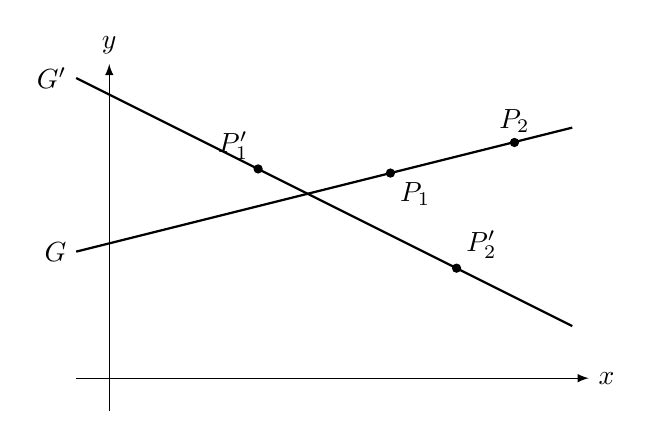
\begin{tikzpicture}[>=latex, scale=1.05]
  \draw[->] (-0.4,0) -- (5.8,0) node[right]{$x$};
  \draw[->] (0,-0.4) -- (0,3.8) node[above]{$y$};
  
  % 直线 G' (负斜率)
  \draw[thick] (-0.4,3.63) -- (5.6,0.63);
  \node[left] at (-0.4,3.63) {$G'$};
  \coordinate (P1p) at (1.8,2.53);
  \coordinate (P2p) at (4.2,1.33);
  \fill (P1p) circle (1.6pt) node[above left]{$P_1'$};
  \fill (P2p) circle (1.6pt) node[above right]{$P_2'$};
  
  % 直线 G (正斜率)
  \draw[thick] (-0.4,1.53) -- (5.6,3.03);
  \node[left] at (-0.4,1.53) {$G$};
  \coordinate (P1) at (3.4,2.48);
  \coordinate (P2) at (4.9,2.85);
  \fill (P1) circle (1.6pt) node[below right]{$P_1$};
  \fill (P2) circle (1.6pt) node[above]{$P_2$};
\end{tikzpicture}
\end{center}

给定两条直线 $G, G' \subset \mathbb{R}^2$, 其中 $G$ 由(不同的)两点 $P_1, P_2 \in \mathbb{R}^2$ 确定, 相应地 $G'$ 由(不同的)两点 $P_1', P_2' \in \mathbb{R}^2$ 确定.于是要根据 $P_1, P_2, P_1', P_2'$ 研究 $G$ 与 $G'$ 是否具有交点, 即公共点, 若有, 又如何从点 $P_1, P_2, P_1', P_2'$ 计算出这些交点.正如我们在第 1 章的预备说明中已经看到的, $G$ 与 $G'$ 具有参数表示

\[
G = \left\{P_1 + t(P_2 - P_1);\; t \in \mathbb{R}\right\}, \qquad
G' = \left\{P_1' + t'(P_2' - P_1');\; t' \in \mathbb{R}\right\},
\]

而交点 $S \in G \cap G'$ 显然刻画为: 存在参数 $t, t' \in \mathbb{R}$ 使得

\[
P_1 + t(P_2 - P_1) = S = P_1' + t'(P_2' - P_1')\text{.}
\]

换言之, 为求 $G$ 与 $G'$ 的交点, 我们必须确定满足方程

\begin{equation}
t(P_2 - P_1) + t'(P_1' - P_2') = P_1' - P_1 \tag{$*$}
\end{equation}

的一切数对 $(t, t') \in \mathbb{R}^2$; 或者, 在分量记号

\[
P_2 - P_1 = (\alpha_{11}, \alpha_{21}), \qquad
P_1' - P_2' = (\alpha_{12}, \alpha_{22}), \qquad
P_1' - P_1 = (\beta_1, \beta_2)
\]

之下, 即满足方程组

\begin{equation}
\begin{array}{c}
t\alpha_{11} + t'\alpha_{12} = \beta_1, \\
t\alpha_{21} + t'\alpha_{22} = \beta_2
\end{array} \tag{$**$}
\end{equation}

的一切数对.于是要解一个由 $2$ 个方程组成的方程组, 其中含两个未知量 $t, t'$ 及给定的常数 $\alpha_{ij}, \beta_i \in \mathbb{R}$.这里涉及的是一个线性方程组, 其含义是: 未知量 $t, t'$ 彼此分离, 且至多以一次幂出现.

为解方程 $(*)$, 我们首先假设两个向量 $P_2 - P_1$ 与 $P_1' - P_2'$ 线性相关, 此时每个向量都是另一个的标量倍; 几何上这意味着 $G$ 与 $G'$ 平行.于是 $P_1' - P_2'$ 是 $P_2 - P_1$ 的一个标量倍, 比如说 $P_1' - P_2' = \gamma(P_2 - P_1)$, 从而可以把方程 $(*)$ 改写为

\[
P_1' = P_1 + (t + \gamma t')(P_2 - P_1)\text{.}
\]

因此解 $t, t'$ 的存在性等价于 $P_1' \in G$, 而这已经蕴含 $G = G'$.于是只可能发生下列互相排斥的情形:

\begin{enumerate}
\item $P_2 - P_1$ 与 $P_1' - P_2'$ 线性相关, $G = G'$;
\item $P_2 - P_1$ 与 $P_1' - P_2'$ 线性相关, $G \neq G'$; 此时 $G \cap G' = \varnothing$;
\item $P_2 - P_1$ 与 $P_1' - P_2'$ 线性无关; 此时 $G$ 与 $G'$ 恰好有一个交点(这是直观明显的), 我们随即就要计算它.
\end{enumerate}

现在我们按情形 3 假设向量 $P_2 - P_1 = (\alpha_{11}, \alpha_{21})$ 与 $P_1' - P_2' = (\alpha_{12}, \alpha_{22})$ 线性无关.特别有 $P_2 - P_1 \neq 0$, 不妨设 $\alpha_{11} \neq 0$.于是我们可以在等价的意义下变换方程组 $(**)$, 即把第一方程的 $\frac{\alpha_{21}}{\alpha_{11}}$ 倍从第二方程中减去, 从而在第二方程中"消去"未知量 $t$:

\[
\begin{array}{r l}
t\alpha_{11} + t'\alpha_{12} &= \beta_1, \\
t'\left(\alpha_{22} - \frac{\alpha_{21}}{\alpha_{11}}\alpha_{12}\right) &= \beta_2 - \frac{\alpha_{21}}{\alpha_{11}}\beta_1\text{.}
\end{array}
\]

但此时 $\alpha_{22} - \frac{\alpha_{21}}{\alpha_{11}}\alpha_{12} \neq 0$, 因为否则将得到

\[
\alpha_{12} = \frac{\alpha_{12}}{\alpha_{11}}\alpha_{11}, \qquad
\alpha_{22} = \frac{\alpha_{12}}{\alpha_{11}}\alpha_{21},
\]

从而 $P_1' - P_2'$ 线性依赖于 $P_2 - P_1$, 这与我们的假设矛盾.于是可以把第二方程继续等价地变换为

\[
t' = \frac{\beta_2 - \frac{\alpha_{21}}{\alpha_{11}}\beta_1}{\alpha_{22} - \frac{\alpha_{21}}{\alpha_{11}}\alpha_{12}}
= \frac{\alpha_{11}\beta_2 - \alpha_{21}\beta_1}{\alpha_{11}\alpha_{22} - \alpha_{21}\alpha_{12}},
\]

并由第一方程得到

\[
t = \frac{1}{\alpha_{11}}\left(\beta_1 - \alpha_{12}\frac{\alpha_{11}\beta_2 - \alpha_{21}\beta_1}{\alpha_{11}\alpha_{22} - \alpha_{21}\alpha_{12}}\right)
= \frac{\beta_1\alpha_{22} - \beta_2\alpha_{12}}{\alpha_{11}\alpha_{22} - \alpha_{21}\alpha_{12}}\text{.}
\]

这里我们是在 $\alpha_{11} \neq 0$ 的假设下对方程作等价变换的, 因此 $t, t'$ 也确实是 $(*)$ 的解.现在还剩下 $\alpha_{11} = 0$ 的情形需要考察.此时必有 $\alpha_{21} \neq 0$, 我们可以在此假设下作相应的计算.关于 $t, t'$ 的结果可以形式上从上面的结果推得: 只需在向量 $(\alpha_{11}, \alpha_{21}), (\alpha_{12}, \alpha_{22}), (\beta_1, \beta_2)$ 中分别交换分量的次序, 这相当于交换方程组 $(**)$ 的两个方程.由于如人们容易看出的, 上面的结果在这种交换下并不改变, 于是得到在非平行直线 $G, G'$ 的情形下, 方程 $(*)$ 亦即线性方程组 $(**)$ 的解为

\[
t = \frac{\beta_1\alpha_{22} - \beta_2\alpha_{12}}{\alpha_{11}\alpha_{22} - \alpha_{21}\alpha_{12}}, \qquad
t' = \frac{\alpha_{11}\beta_2 - \alpha_{21}\beta_1}{\alpha_{11}\alpha_{22} - \alpha_{21}\alpha_{12}}\text{.}
\]

特别地, $G \cap G'$ 恰由一个交点组成, 它分别作为 $G$ 与 $G'$ 的点由

\[
S = P_1 + \frac{\beta_1\alpha_{22} - \beta_2\alpha_{12}}{\alpha_{11}\alpha_{22} - \alpha_{21}\alpha_{12}}(P_2 - P_1)
= P_1' + \frac{\alpha_{11}\beta_2 - \alpha_{21}\beta_1}{\alpha_{11}\alpha_{22} - \alpha_{21}\alpha_{12}}(P_2' - P_1')
\]

计算出来.

类似地, 求 $\mathbb{R}^3$ 中两个平面的交, 或更一般地求 $K^n$ 中两个仿射子空间的交, 都归结为线性方程组.前一种情形例如是含 $4$ 个未知量的 $3$ 个方程组成的方程组, 其中在一般情况下有一个未知量可自由选取, 从而交被参数化为一条直线.后一种情形要考虑含 $r + s$ 个未知量的 $n$ 个方程组成的方程组, 其中 $r$ 与 $s$ 是所考察的 $K^n$ 中仿射子空间的维数.

甚至关于向量空间中向量的直接问题也可能导致线性方程组.例如在域 $K$ 上考虑向量 $a_i = (\alpha_{1i}, \ldots, \alpha_{ni}) \in K^n$, $i = 1, \ldots, r$, 检验它们是否线性相关.于是我们必须判断是否存在不全为零的元素 $t_1, \ldots, t_r \in K$ 使得

\[
t_1 a_1 + \cdots + t_r a_r = 0
\]

成立; 或者, 转到各个分量, 线性方程组

\[
\begin{array}{c}
t_1\alpha_{11} + \cdots + t_r\alpha_{1r} = 0, \\
t_1\alpha_{21} + \cdots + t_r\alpha_{2r} = 0, \\
\cdots \\
t_1\alpha_{n1} + \cdots + t_r\alpha_{nr} = 0
\end{array}
\]

是否具有非平凡解 $t_1, \ldots, t_r \in K$.或者我们考虑把标准基(由单位向量 $e_1, \ldots, e_r \in K^r$ 组成)映到向量 $a_1, \ldots, a_r \in K^n$ 的线性映射 $f \colon K^r \longrightarrow K^n$, 然后问: 给定的向量 $b = (\beta_1, \ldots, \beta_n)$ 是否属于 $f$ 的像, 即属于由向量 $a_i = f(e_i)$, $i = 1, \ldots, r$ 生成的子空间.因此要检验的是方程

\[
t_1 a_1 + \cdots + t_r a_r = b
\]

是否可解; 或就 $a_i = (\alpha_{1i}, \ldots, \alpha_{ni})$, $i = 1, \ldots, r$ 而言, 线性方程组

\[
\begin{array}{c}
t_1\alpha_{11} + \cdots + t_r\alpha_{1r} = \beta_1, \\
t_1\alpha_{21} + \cdots + t_r\alpha_{2r} = \beta_2, \\
\cdots \\
t_1\alpha_{n1} + \cdots + t_r\alpha_{nr} = \beta_n
\end{array}
\]

是否允许一个解.

上述方程组中系数的排列方式提示我们, 不再把向量 $a_1, \ldots, a_r, b$ 写成行向量, 而写成列向量, 即

\[
a_1 = \begin{pmatrix} \alpha_{11} \\ \vdots \\ \alpha_{n1} \end{pmatrix}, \quad
\ldots, \quad
a_r = \begin{pmatrix} \alpha_{1r} \\ \vdots \\ \alpha_{nr} \end{pmatrix}, \quad
b = \begin{pmatrix} \beta_1 \\ \vdots \\ \beta_n \end{pmatrix}\text{.}
\]

此外我们将考察矩形的系数表

\[
A = (a_1, \ldots, a_r) =
\begin{pmatrix}
\alpha_{11} & \cdots & \alpha_{1r} \\
\alpha_{21} & \cdots & \alpha_{2r} \\
\vdots & \ddots & \vdots \\
\alpha_{n1} & \cdots & \alpha_{nr}
\end{pmatrix},
\]

并称之为方程组的\emph{系数矩阵}(\textup{Koeffizientenmatrix})\index{xishujuzhen@系数矩阵(Koeffizientenmatrix)}.我们还要把未知量 $t_1, \ldots, t_r$ 合成为一个列向量, 从而可以像一元方程的情形那样, 把上面的线性方程组写成清晰的形式

\[
\begin{pmatrix}
\alpha_{11} & \cdots & \alpha_{1r} \\
\alpha_{21} & \cdots & \alpha_{2r} \\
\vdots & \ddots & \vdots \\
\alpha_{n1} & \cdots & \alpha_{nr}
\end{pmatrix}
\cdot
\begin{pmatrix} t_1 \\ \vdots \\ t_r \end{pmatrix}
=
\begin{pmatrix} \beta_1 \\ \vdots \\ \beta_n \end{pmatrix},
\]

其中系数矩阵与未知量向量的乘积定义为

\[
\begin{pmatrix}
\alpha_{11} & \cdots & \alpha_{1r} \\
\alpha_{21} & \cdots & \alpha_{2r} \\
\vdots & \ddots & \vdots \\
\alpha_{n1} & \cdots & \alpha_{nr}
\end{pmatrix}
\cdot
\begin{pmatrix} t_1 \\ \vdots \\ t_r \end{pmatrix}
:=
\begin{pmatrix}
\sum_{j = 1}^{r}\alpha_{1j}t_j \\
\vdots \\
\sum_{j = 1}^{r}\alpha_{nj}t_j
\end{pmatrix}\text{.}
\]

于是方程组仍写作

\[
\sum_{j = 1}^{r}\alpha_{ij}t_j = \beta_i, \qquad i = 1, \ldots, n,
\]

其中正如这里所做的, 今后我们总是把系数 $\alpha_{ij}$ 写在未知量 $t_j$ 的左边.

矩阵作为矩形系数表的意义并不局限于线性方程组.在线性代数中, 凡是要对依赖于两个指标参数的标量加以编排的地方, 都会出现矩阵.例如考虑 $K$-向量空间 $V, W$ 之间带有基 $X = (x_1, \ldots, x_r)$ 与 $Y = (y_1, \ldots, y_n)$ 的线性映射 $f \colon V \longrightarrow W$.此时 $f$ 完全由基 $X$ 的像 $f(x_1), \ldots, f(x_r)$ 所刻画.而每个这样的像 $f(x_j)$ 又完全由它在 $Y$ 下的坐标所刻画, 即由把 $f(x_j)$ 表示为基 $Y$ 的线性组合所需的系数 $\alpha_{1j}, \ldots, \alpha_{nj} \in K$ 所刻画, 例如

\[
f(x_j) = \sum_{i = 1}^{n}\alpha_{ij}y_i, \qquad j = 1, \ldots, r\text{.}
\]

于是 $f$ 由矩阵

\[
A_{f, X, Y} =
\begin{pmatrix}
\alpha_{11} & \cdots & \alpha_{1r} \\
\alpha_{21} & \cdots & \alpha_{2r} \\
\vdots & \ddots & \vdots \\
\alpha_{n1} & \cdots & \alpha_{nr}
\end{pmatrix}
\]

唯一刻画, 我们称之为描述 $f$ 关于 $V$ 的基 $X$ 与 $W$ 的基 $Y$ 的矩阵.对应 $f \longmapsto A_{f, X, Y}$ 具有非常好的性质, 我们后面会看到.例如, 从向量 $x \in V$ 到它的像 $f(x) \in W$ 的过渡, 在关于 $X$ 与 $Y$ 的坐标层面上, 可以解释为 $A_{f, X, Y}$ 与 $x$ 关于 $X$ 的所谓\emph{坐标列向量}(\textup{Koordinatenspaltenvektor})\index{zuobiaoliexiangliang@坐标列向量(Koordinatenspaltenvektor)}的乘积.进一步, 线性映射的复合在选用合适基的情形下, 恰好对应描述\emph{矩阵的乘积}(\textup{Produkt von Matrizen})\index{juzhendechengji@矩阵的乘积(Produkt von Matrizen)}(这一乘积我们即将定义).

在特殊情形 $V = W$ 且 $f = \mathrm{id}$ 下, 矩阵 $A_{\mathrm{id}, X, Y}$ 恰好提供了把基 $X$ 的元素表示为基 $Y$ 的线性组合所需的系数.特别地我们看到, 向量空间不同基之间的变换也借助矩阵来描述.矩阵的另一个应用领域是第 7 章将要处理的数量积.

在本章中, 我们首先更仔细地研究线性映射 $f$ 与其\emph{描述矩阵}(\textup{beschreibende Matrix})\index{miaoshujuzhen@描述矩阵(beschreibende Matrix)} $A_{f, X, Y}$ 之间的对应关系.然后讨论\emph{高斯消元法}(\textup{Gauß'sches Eliminationsverfahren})\index{gaosixiaoyuanfa@高斯消元法(Gauß'sches Eliminationsverfahren)}, 首先把它作为借助所谓\emph{初等行变换}(\textup{elementare Zeilenumformungen})\index{chudengahngbianhuan@初等行变换(elementare Zeilenumformungen)}确定矩阵\emph{行秩}(\textup{Zeilenrang})\index{hangzhi@行秩(Zeilenrang)}的方法, 这里行秩即由矩阵的各行生成的向量空间的维数.类似地可以考察矩阵的\emph{列秩}(\textup{Spaltenrang})\index{liezhi@列秩(Spaltenrang)}.容易看出, 对于属于线性映射 $f$ 的矩阵 $A_{f, X, Y}$, 列秩与 $f$ 的秩, 即 $f$ 的像的维数一致.然而, 矩阵的列秩是否总与它的行秩一致, 却是一个非平凡的结果.

接下来我们处理(方)矩阵的可逆性.方阵 $A$ 称为可逆的, 如果存在方阵 $B$ 使得 $A \cdot B = B \cdot A = E$, 其中 $E$ 表示所谓\emph{单位矩阵}(\textup{Einheitsmatrix})\index{danweijuzhen@单位矩阵(Einheitsmatrix)}, 它的对角线元素全为 $1$, 其余元素全为 $0$.我们尤其会看到, 线性映射是同构的性质, 在矩阵这一边对应可逆性.此外, 我们利用高斯消元法来检验具体给出的矩阵是否可逆, 并在可能时求出其逆.随后给出\emph{可逆矩阵}(\textup{invertierbare Matrix})\index{kenijuzhen@可逆矩阵(invertierbare Matrix)}在\emph{基变换}(\textup{Basiswechsel})\index{jibianhuan@基变换(Basiswechsel)}矩阵框架下的解释.

最后我们还要详细讨论线性方程组.我们把它纳入线性映射的框架中, 并特别说明如何用高斯消元法把具体给定方程组的求解形式化.

\section{线性映射与矩阵}\index{xianxingyingshe@线性映射(lineare Abbildung)}\index{juzhen@矩阵(Matrix)}\label{sec:3.1}

我们已经在 \ref{sec:2.1} 节看到, 可以借助矩阵定义线性映射, 反之线性映射可以关于所选取的基用矩阵来描述.这一事实要在本节中作更仔细的研究.照例设 $K$ 是一个域.

\begin{definition}[$(m \times n)$-矩阵]\label{def:3.1.1}\index{juzhen@矩阵(Matrix)}
设 $m, n \in \mathbb{N}$.一个系数在 $K$ 中的 $(m \times n)$-矩阵是元素 $\alpha_{ij} \in K$ 的一个系统, 其中 $(i, j) \in \{1, \ldots, m\} \times \{1, \ldots, n\}$, 即
\[
A = (\alpha_{ij})_{\substack{i = 1, \ldots, m\\ j = 1, \ldots, n}} =
\begin{pmatrix}
\alpha_{11} & \cdots & \alpha_{1n} \\
\vdots & \ddots & \vdots \\
\alpha_{m1} & \cdots & \alpha_{mn}
\end{pmatrix}\text{.}
\]
这里 $i$ 称为 $A$ 的行指标; 在写法
\[
A = (\alpha_{ij})_{\substack{i = 1, \ldots, m\\ j = 1, \ldots, n}} \qquad \text{或} \qquad A = (\alpha_{ij})_{i, j}
\]
中, 可以这样辨认行指标: 它写在包围括号之外的第一位置.相应地, 作为第二个指标的 $j$ 是 $A$ 的列指标.于是 $A$ 由 $m$ 行与 $n$ 列组成.对于 $m = 0$ 或 $n = 0$, $A$ 是所谓\emph{空矩阵}(\textup{leere Matrix})\index{kongjuzhen@空矩阵(leere Matrix)}\footnote{即行数或列数为零的矩阵.}.
\end{definition}

我们用 $K^{m \times n}$ 表示一切 $(m \times n)$-矩阵的集合.在对应

\[
\begin{pmatrix}
\alpha_{11} & \cdots & \alpha_{1n} \\
\vdots & \ddots & \vdots \\
\alpha_{m1} & \cdots & \alpha_{mn}
\end{pmatrix}
\longmapsto
(\alpha_{11}, \ldots, \alpha_{1n}, \alpha_{21}, \ldots, \alpha_{2n}, \ldots, \alpha_{m1}, \ldots, \alpha_{mn})
\]

之下, $K^{m \times n}$ 可以与 $K^{m \cdot n}$ 等同.特别地, 与 $K^{m \cdot n}$ 一样, 我们可以把 $K^{m \times n}$ 看作 $K$-向量空间.于是对矩阵

\[
A = (\alpha_{ij})_{i, j}, \quad B = (\beta_{ij})_{i, j} \in K^{m \times n}
\]

它们的和定义为

\[
A + B = (\alpha_{ij} + \beta_{ij})_{i, j},
\]

$A$ 与标量 $\lambda \in K$ 的乘积定义为

\[
\lambda A = (\lambda\alpha_{ij})_{i, j}\text{.}
\]

零元 $0 \in K^{m \times n}$ 是所谓\emph{零矩阵}(\textup{Nullmatrix})\index{lingjuzhen@零矩阵(Nullmatrix)}, 它的系数 $\alpha_{ij}$ 全都为零.特别地, 矩阵 $A = (\alpha_{ij})_{i, j} \in K^{m \times n}$ 的负元是矩阵 $-A = (-\alpha_{ij})_{i, j}$.$K^{m \times n}$ 的标准基由矩阵

\[
E_{ij} = (\delta_{i\mu}\delta_{j\nu})_{\substack{\mu = 1, \ldots, m\\ \nu = 1, \ldots, n}}, \qquad i = 1, \ldots, m, \quad j = 1, \ldots, n,
\]

给出, 其中 $E_{ij}$ 在 $i$ 行与 $j$ 列的交点处为 $1$, 其余全为 $0$.例如对矩阵 $(\alpha_{ij})_{i, j} \in K^{m \times n}$ 有

\[
A = \sum_{\substack{i = 1, \ldots, m\\ j = 1, \ldots, n}}\alpha_{ij}E_{ij}\text{.}
\]

在矩阵的语境中, 人们习惯于不再像迄今那样把向量 $a \in K^m$ 写成行向量 $a = (\alpha_1, \ldots, \alpha_m)$, 而写成列向量:

\[
a = \begin{pmatrix} \alpha_1 \\ \vdots \\ \alpha_m \end{pmatrix}\text{.}
\]

特别地, 可以由 $n$ 个这样的向量 $a_1, \ldots, a_n \in K^m$ 构成一个矩阵 $A = (a_1, \ldots, a_n) \in K^{m \times n}$.若 $W$ 是带基 $Y = (y_1, \ldots, y_m)$ 的有限维 $K$-向量空间, 则每个 $a \in W$ 都有表示 $a = \sum_{i = 1}^{m}\alpha_i y_i$, 其中系数 $\alpha_i \in K$ 唯一确定.我们把

\[
a_Y = \begin{pmatrix} \alpha_1 \\ \vdots \\ \alpha_m \end{pmatrix} \in K^m
\]

称为属于 $a \in W$,关于 $W$ 的基 $Y$ 的坐标列向量.

\begin{remark}\label{rem:3.1.2}
设 $W$ 是带基 $Y = (y_1, \ldots, y_m)$ 的 $K$-向量空间.则映射
\[
\kappa_Y \colon W \longrightarrow K^m, \qquad a \longmapsto a_Y,
\]
是 $K$-向量空间的同构.
\end{remark}

\begin{proof}
容易直接验证 $\kappa_Y$ 是线性的, 并把 $W$ 的基 $Y$ 映到 $K^m$ 的标准基.于是 $\kappa_Y$ 必为同构.
\end{proof}

利用坐标列向量, 我们可以用简单的方式刻画在 \ref{sec:2.1} 节已提及的,把一个矩阵分配给一个线性映射的对应关系:

\begin{definition}[线性映射的矩阵]\label{def:3.1.3}\index{juzhen@矩阵(Matrix)}
设 $V, W$ 是 $K$-向量空间, 分别带有基 $X = (x_1, \ldots, x_n)$ 与 $Y = (y_1, \ldots, y_m)$.若 $f \colon V \longrightarrow W$ 是 $K$-线性映射, 则
\[
A = A_{f, X, Y} = \left(f(x_1)_Y, \ldots, f(x_n)_Y\right) \in K^{m \times n}
\]
称为 $f$ 关于基 $X$ 与 $Y$ 的矩阵.
\end{definition}

属于 $f$ 的矩阵 $A_{f, X, Y}$ 恰好由关于 $Y$ 的,从 $V$ 的基 $x_1, \ldots, x_n$ 的像 $f(x_1), \ldots, f(x_n)$ 得到的坐标列向量组成.为了把 $A_{f, X, Y}$ 明确地写出来, 用基 $Y$ 表示 $x_1, \ldots, x_n$ 的像, 例如

\[
f(x_j) = \sum_{i = 1}^{m}\alpha_{ij}y_i, \qquad j = 1, \ldots, n,
\]

则有:

\[
A_{f, X, Y} =
\begin{pmatrix}
\alpha_{11} & \cdots & \alpha_{1n} \\
\vdots & \ddots & \vdots \\
\alpha_{m1} & \cdots & \alpha_{mn}
\end{pmatrix}\text{.}
\]

例如属于零映射 $0 \colon V \longrightarrow W$ 的矩阵 $A_{0, X, Y}$ 恰是零矩阵 $0 \in K^{m \times n}$.另一方面, 若在 $V = W$ 且 $X = Y$ 的情形考察恒等映射 $\mathrm{id} \colon V \longrightarrow V$, 则相应的矩阵 $A_{\mathrm{id}, X, X}$ 是所谓 $(m \times m)$-单位矩阵:

\[
E := E_m := (\delta_{ij})_{i, j = 1, \ldots, m} =
\begin{pmatrix}
1 & 0 & 0 & \cdots & 0 \\
0 & 1 & 0 & \cdots & 0 \\
0 & 0 & 1 & \cdots & 0 \\
\vdots & \vdots & \vdots & \ddots & \vdots \\
0 & 0 & 0 & \cdots & 1
\end{pmatrix} \in K^{m \times m}\text{.}
\]

现在我们更仔细地研究对应 $f \longmapsto A_{f, X, Y}$, 并回忆: $K$-向量空间 $V$ 到 $K$-向量空间 $W$ 的一切 $K$-线性映射的集合又构成一个 $K$-向量空间, 记作 $\operatorname{Hom}_K(V, W)$.两个元素 $f, g \in \operatorname{Hom}_K(V, W)$ 的和定义为 $(f + g)(a) = f(a) + g(a)$, $f$ 与元素 $\alpha \in K$ 的标量倍定义为 $(\alpha f)(a) = \alpha f(a)$, 均对 $a \in V$ 而言.

\begin{theorem}\label{thm:3.1.4}
设 $V, W$ 是带有给定基 $X = (x_1, \ldots, x_n)$ 与 $Y = (y_1, \ldots, y_m)$ 的有限维 $K$-向量空间.则映射
\[
\varPsi \colon \operatorname{Hom}_K(V, W) \longrightarrow K^{m \times n}, \qquad f \longmapsto A_{f, X, Y},
\]
是 $K$-向量空间的同构.
\end{theorem}

\begin{proof}
我们先验证 $\varPsi$ 是 $K$-线性的.为此利用同构 $W \longrightarrow K^m$, $a \longmapsto a_Y$, 特别是利用这一映射是 $K$-线性的.对 $f, g \in \operatorname{Hom}_K(V, W)$, $\alpha \in K$ 有
\[
\begin{array}{l}
A_{f + g, X, Y} = \left((f + g)(x_1)_Y, \ldots, (f + g)(x_n)_Y\right) \\
\qquad = \left(\left(f(x_1) + g(x_1)\right)_Y, \ldots, \left(f(x_n) + g(x_n)\right)_Y\right) \\
\qquad = \left(f(x_1)_Y + g(x_1)_Y, \ldots, f(x_n)_Y + g(x_n)_Y\right) \\
\qquad = \left(f(x_1)_Y, \ldots, f(x_n)_Y\right) + \left(g(x_1)_Y, \ldots, g(x_n)_Y\right) \\
\qquad = A_{f, X, Y} + A_{g, X, Y},
\end{array}
\]
以及
\[
\begin{array}{l}
A_{(\alpha f), X, Y} = \left((\alpha f)(x_1)_Y, \ldots, (\alpha f)(x_n)_Y\right) \\
\qquad = \left(\alpha\left(f(x_1)\right)_Y, \ldots, \alpha\left(f(x_n)\right)_Y\right) \\
\qquad = \alpha\left(f(x_1)_Y, \ldots, f(x_n)_Y\right) \\
\qquad = \alpha \cdot A_{f, X, Y},
\end{array}
\]
即 $\varPsi(f + g) = \varPsi(f) + \varPsi(g)$, $\varPsi(\alpha f) = \alpha\varPsi(f)$, 也就是说 $\varPsi$ 是 $K$-线性的.再由定理~\mtref{thm:2.1.7} (i) 得 $\varPsi$ 单射, 由定理~\mtref{thm:2.1.7} (ii) 得 $\varPsi$ 满射.
\end{proof}

\begin{corollary}\label{cor:3.1.5}
对有限维 $K$-向量空间 $V, W$ 有
\[
\dim_K \operatorname{Hom}_K(V, W) = \dim_K V \cdot \dim_K W\text{.}
\]
\end{corollary}

下面我们来定义矩阵的乘积, 并证明它对应线性映射的复合.对自然数 $m, n, p \in \mathbb{N}$, 可以把矩阵 $A \in K^{m \times n}$ 与矩阵 $B \in K^{n \times p}$ 相乘, 得到 $K^{m \times p}$ 中的矩阵.确切地说, 对

\[
A = (\alpha_{ij})_{\substack{i = 1, \ldots, m\\ j = 1, \ldots, n}} \in K^{m \times n}, \qquad
B = (\beta_{jk})_{\substack{j = 1, \ldots, n\\ k = 1, \ldots, p}} \in K^{n \times p},
\]

乘积 $A \cdot B$ 定义为:

\[
A \cdot B = \left(\sum_{j = 1}^{n}\alpha_{ij} \cdot \beta_{jk}\right)_{\substack{i = 1, \ldots, m\\ k = 1, \ldots, p}}\text{.}
\]

乘积只有当 $A$ 的列数等于 $B$ 的行数时才能构成.矩阵乘积的一个简单情形是把 $K^{1 \times m}$ 中的一行与 $K^{m \times 1}$ 中的一列相乘:

\[
(\alpha_1, \ldots, \alpha_m) \cdot
\begin{pmatrix} \beta_1 \\ \vdots \\ \beta_m \end{pmatrix}
= (\alpha_1\beta_1 + \cdots + \alpha_m\beta_m)\text{.}
\]

得到的是一 $(1 \times 1)$-矩阵, 我们约定去掉括号, 把它与 $K$ 中相应的元素等同.因此可以说, 对矩阵 $A \in K^{m \times n}$, $B \in K^{n \times p}$, 乘积 $A \cdot B = (\gamma_{ik})_{i, k}$ 由 $A$ 的各行与 $B$ 的各列的全部乘积组成: 具体地说, $A \cdot B$ 的第 $i$ 行第 $k$ 列处的元素 $\gamma_{ik}$ 恰是 $A$ 的第 $i$ 行与 $B$ 的第 $k$ 列的乘积.另一方面要注意, $K^{m \times 1}$ 中的一列与 $K^{1 \times n}$ 中的一行的乘积给出 $K^{m \times n}$ 中的矩阵:

\[
\begin{pmatrix} \alpha_1 \\ \vdots \\ \alpha_m \end{pmatrix}
\cdot
(\beta_1, \ldots, \beta_n)
=
\begin{pmatrix}
\alpha_1\beta_1 & \cdots & \alpha_1\beta_n \\
\vdots & \ddots & \vdots \\
\alpha_m\beta_1 & \cdots & \alpha_m\beta_n
\end{pmatrix}\text{.}
\]

\begin{remark}[矩阵乘法的结合律]\label{rem:3.1.6}
矩阵乘法满足结合律, 即对 $m, n, p, q \in \mathbb{N}$ 及矩阵 $A \in K^{m \times n}$, $B \in K^{n \times p}$, $C \in K^{p \times q}$ 恒有
\[
(A \cdot B) \cdot C = A \cdot (B \cdot C)\text{.}
\]
\end{remark}

\begin{proof}
令 $A = (\alpha_{ij})_{\substack{i = 1, \ldots, m\\ j = 1, \ldots, n}}$, $B = (\beta_{jk})_{\substack{j = 1, \ldots, n\\ k = 1, \ldots, p}}$, $C = (\gamma_{k\ell})_{\substack{k = 1, \ldots, p\\ \ell = 1, \ldots, q}}$.则
\[
(A \cdot B) \cdot C = \left(\sum_{j = 1}^{n}\alpha_{ij}\beta_{jk}\right)_{i, k} \cdot C
= \left(\sum_{k = 1}^{p}\sum_{j = 1}^{n}\alpha_{ij}\beta_{jk}\gamma_{k\ell}\right)_{i, \ell},
\]
\[
A \cdot (B \cdot C) = A \cdot \left(\sum_{k = 1}^{p}\beta_{jk}\gamma_{k\ell}\right)_{j, \ell}
= \left(\sum_{j = 1}^{n}\sum_{k = 1}^{p}\alpha_{ij}\beta_{jk}\gamma_{k\ell}\right)_{i, \ell},
\]
即如所愿 $(A \cdot B) \cdot C = A \cdot (B \cdot C)$.
\end{proof}

现在我们要在线性映射的意义下解释矩阵.首先应当指出, 每个矩阵 $A = (\alpha_{ij})_{i, j} \in K^{m \times n}$ 都给出一个映射

\[
f \colon K^n \longrightarrow K^m, \qquad x \longmapsto A \cdot x,
\]

其中我们把 $K^n$ 与 $K^{n \times 1}$,$K^m$ 与 $K^{m \times 1}$ 等同.详细写出来, 映射法则为

\[
\begin{pmatrix} \xi_1 \\ \vdots \\ \xi_n \end{pmatrix}
\longmapsto
\begin{pmatrix}
\sum_{j = 1}^{n}\alpha_{1j}\xi_j \\
\vdots \\
\sum_{j = 1}^{n}\alpha_{mj}\xi_j
\end{pmatrix},
\]

由此立即可见 $f$ 是 $K$-线性的.若在 $K^n$ 与 $K^m$ 中分别采用由单位向量组成的标准基, 则 $A$ 显然正是按定义~\mtref{def:3.1.3} 属于 $f$ 的矩阵.我们要证明, 这个例子在某种意义下已经描述了普遍情形:

\begin{theorem}\label{thm:3.1.7}
设 $f \colon V \longrightarrow W$ 是带基 $X = (x_1, \ldots, x_n)$ 与 $Y = (y_1, \ldots, y_m)$ 的向量空间 $V$ 与 $W$ 之间的 $K$-线性映射.则对 $a \in V$ 有
\[
f(a)_Y = A_{f, X, Y} \cdot a_X\text{.}
\]
\end{theorem}

\begin{proof}
设 $A_{f, X, Y} = (\alpha_{ij})_{i, j}$, $a_X = (\xi_j)$.则
\[
f(x_j) = \sum_{i = 1}^{m}\alpha_{ij}y_i, \qquad j = 1, \ldots, n,
\]
并且 $a = \sum_{j = 1}^{n}\xi_j x_j$.于是
\[
f(a) = \sum_{j = 1}^{n}\xi_j f(x_j) = \sum_{j = 1}^{n}\xi_j\sum_{i = 1}^{m}\alpha_{ij}y_i
= \sum_{i = 1}^{m}\left(\sum_{j = 1}^{n}\alpha_{ij}\xi_j\right)y_i,
\]
即如所愿 $f(a)_Y = A_{f, X, Y} \cdot a_X$.
\end{proof}

定理~\mtref{thm:3.1.7} 的公式尤其可以应用于 $V = W$ 与恒等映射 $\mathrm{id} \colon V \longrightarrow V$ 的情形.此时它描述一个基变换, 并表明如何把关于基 $X$ 的坐标向量换算为关于基 $Y$ 的坐标向量:

\[
a_Y = A_{\mathrm{id}, X, Y} \cdot a_X\text{.}
\]

为了把定理~\mtref{thm:3.1.7} 的断言解释得更精确些, 我们引入映射 $\kappa_X \colon V \longrightarrow K^n$, $a \longmapsto a_X$ 与 $\kappa_Y \colon W \longrightarrow K^m$, $b \longmapsto b_Y$, 它们分别把向量送到相应的坐标列向量; 由注记~\mtref{rem:3.1.2}, $\kappa_X$ 与 $\kappa_Y$ 是 $K$-向量空间的同构.再设 $\tilde{f} \colon K^n \longrightarrow K^m$ 由 $x \longmapsto A_{f, X, Y} \cdot x$ 给出.则定理~\mtref{thm:3.1.7} 中的公式恰好说明:

\begin{corollary}\label{cor:3.1.8}
在前述情形下, 下图
\begin{center}
\begin{tikzcd}
V \arrow[r, "f"] \arrow[d, "\kappa_X"'] & W \arrow[d, "\kappa_Y"] \\
K^n \arrow[r, "\tilde{f}"'] & K^m
\end{tikzcd}
\end{center}
可交换.
\end{corollary}

因此若把映射 $\kappa_X, \kappa_Y$ 视为等同, 则 $f$ 变为 $\tilde{f}$, 无非就是与矩阵 $A_{f, X, Y}$ 相乘.

下面我们要证明, 矩阵乘积可以解释为线性映射的复合.

\begin{theorem}\label{thm:3.1.9}
设 $U, V, W$ 是带基 $X, Y, Z$ 的有限维 $K$-向量空间.则对线性映射 $f \colon U \longrightarrow V$ 与 $g \colon V \longrightarrow W$ 有
\[
A_{g \circ f, X, Z} = A_{g, Y, Z} \cdot A_{f, X, Y}\text{.}
\]
\end{theorem}

\begin{proof}
这个公式也容易验证.设
\[
X = (x_1, \ldots, x_p), \qquad Y = (y_1, \ldots, y_n), \qquad Z = (z_1, \ldots, z_m),
\]
且
\[
A_{f, X, Y} = (\alpha_{jk})_{\substack{j = 1, \ldots, n\\ k = 1, \ldots, p}}, \qquad
A_{g, Y, Z} = (\beta_{ij})_{\substack{i = 1, \ldots, m\\ j = 1, \ldots, n}}\text{.}
\]
则对 $k = 1, \ldots, p$ 有 $f(x_k) = \sum_{j = 1}^{n}\alpha_{jk}y_j$, 从而
\[
\begin{array}{l}
g \circ f(x_k) = \sum_{j = 1}^{n}\alpha_{jk}g(y_j) \\
\qquad = \sum_{j = 1}^{n}\alpha_{jk}\sum_{i = 1}^{m}\beta_{ij}z_i \\
\qquad = \sum_{i = 1}^{m}\left(\sum_{j = 1}^{n}\beta_{ij}\alpha_{jk}\right)z_i,
\end{array}
\]
即
\[
A_{g \circ f, X, Z} = \left(\sum_{j = 1}^{n}\beta_{ij}\alpha_{jk}\right)_{i, k} = A_{g, Y, Z} \cdot A_{f, X, Y},
\]
如所愿.
\end{proof}

但我们也可以换一种方式证明, 从而完全省去计算.因为由推论~\mtref{cor:3.1.8} 有可交换图表

\begin{center}
\begin{tikzcd}[column sep=1.6em, row sep=1.6em]
U \arrow[r, "f"] \arrow[d, "\kappa_X"'] & V \arrow[r, "g"] \arrow[d, "\kappa_Y"'] & W \arrow[d, "\kappa_Z"] \\
K^p \arrow[r, "\tilde{f}"'] & K^n \arrow[r, "\tilde{g}"'] & K^m
\end{tikzcd}
\end{center}

其中 $\tilde{f}$ 由 $x \longmapsto A_{f, X, Y} \cdot x$,$\tilde{g}$ 由 $y \longmapsto A_{g, Y, Z} \cdot y$ 定义.由注记~\mtref{rem:3.1.6} 可见, $A_{g \circ f, X, Z}$ 与 $A_{g, Y, Z} \cdot A_{f, X, Y}$ 是描述 $K$-线性映射 $g \circ f$ 关于基 $X$ 与 $Z$ 的两个矩阵.于是由定理~\mtref{thm:3.1.4} 得 $A_{g \circ f, X, Z} = A_{g, Y, Z} \cdot A_{f, X, Y}$.

最后我们列出若干矩阵运算规则, 它们容易通过直接验证来检验; 另见注记~\mtref{rem:3.1.6}.设 $\alpha \in K$, $A, B, C$ 是系数在 $K$ 中的矩阵.再设 $0$ 表示零矩阵, $E$ 表示(方)单位矩阵.则下列公式成立:

\[
\begin{array}{c}
A + B = B + A, \\
A + 0 = A, \\
EA = A, \quad BE = B, \\
(\alpha A)B = A(\alpha B) = \alpha(AB), \\
A(B + C) = AB + AC, \\
(A + B)C = AC + BC, \\
(AB)C = A(BC),
\end{array}
\]

其中在各条等式中我们要求行数或列数取得使所列出的和与积能够构成.因此在加法与乘法的意义下, 可以(几乎)像往常一样用矩阵计算.不过在一个乘积 $AB$ 中不得交换因子, 即使对矩阵 $A, B$, 乘积 $AB$ 与 $BA$ 都已定义也不行; 例如考察各含 $n$ 个分量的一行 $A$ 与一列 $B$.甚至对方阵, 即行数与列数相等的矩阵, 乘积 $AB$ 一般也不同于 $B \cdot A$, 用简单例子即可检验.

\aufgaben

\noindent\textbf{习题 1.} 计算矩阵
\[
A = \begin{pmatrix} 1 & 2 \\ 3 & -1 \end{pmatrix}, \qquad
B = \begin{pmatrix} 2 & 0 \\ 1 & 1 \end{pmatrix} \quad \in \mathbb{R}^{2 \times 2}
\]
的乘积 $AB$ 与 $BA$.

\noindent\textbf{习题 2.} 在所指明的 $K$-向量空间 $V$ 中选取一个标准基 $X$, 并对线性映射 $f \colon V \longrightarrow V$ 分别求出相应的矩阵 $A_{f, X, X}$.
\begin{enumerate}
\item[(i)] $V = \mathbb{R}^2$, $K = \mathbb{R}$, $f$ 为在数学正方向上的 $90^\circ$ 旋转;
\item[(ii)] $V = \mathbb{R}^2$, $K = \mathbb{R}$, $f$ 为关于直线 $y = x$ 的反射;
\item[(iii)] $V = \mathbb{Q}(\sqrt{2})$, $K = \mathbb{Q}$, $f$ 为与 $\alpha + \beta\sqrt{2}$ 相乘, 其中 $\alpha, \beta \in \mathbb{Q}$.
\end{enumerate}

\noindent\textbf{习题 3.} 设 $K$ 是一个域.证明映射
\[
f \colon K \longrightarrow K^{2 \times 2}, \qquad x \longmapsto \begin{pmatrix} 1 & x \\ 0 & 1 \end{pmatrix}
\]
是单射, 并且对 $x, y \in K$ 满足关系 $f(x + y) = f(x) \cdot f(y)$.

\noindent\textbf{习题 4.} 设 $f \colon V \longrightarrow W$ 是有限维 $K$-向量空间之间的 $K$-线性映射, 且 $\operatorname{rg} f = r$.证明: 存在 $V$ 的基 $X$ 与 $W$ 的基 $Y$, 使得属于 $f$ 的矩阵 $A_{f, X, Y}$ 具有如下形式:
\[
A_{f, X, Y} = \begin{pmatrix} E_r & 0 \\ 0 & 0 \end{pmatrix}\text{.}
\]
其中 $E_r$ 表示 $(r \times r)$-单位矩阵, 而 $0$ 各表示合适的零矩阵.(AT 314)

\noindent\textbf{习题 5.} 对 $m_1, m_2, n_1, n_2 \in \mathbb{N} - \{0\}$ 考察矩阵
\[
A \in K^{m_1 \times n_1}, \quad B \in K^{m_1 \times n_2}, \quad C \in K^{m_2 \times n_1}, \quad D \in K^{m_2 \times n_2}, \quad E \in K^{n_1 \times r}, \quad F \in K^{n_2 \times r},
\]
并证明
\[
\begin{pmatrix} A & B \\ C & D \end{pmatrix}
\binom{E}{F} = \binom{AE + BF}{CE + DF},
\]
其中把这个等式以显然的方式理解为 $K^{(m_1 + m_2) \times r}$ 中矩阵之间的等式.

\noindent\textbf{习题 6.} 设 $V$ 是有限维 $K$-向量空间, $f \colon V \longrightarrow V$ 是自同态.证明:
\begin{enumerate}
\item[(i)] 恰当存在非平凡线性子空间 $U \subset V$ 满足 $f(U) \subset U$ 时, 才存在 $V$ 的基 $X$ 使得
\[
A_{f, X, X} = \begin{pmatrix} * & * \\ 0 & * \end{pmatrix};
\]
\item[(ii)] 恰当存在非平凡线性子空间 $U_1, U_2 \subset V$ 满足 $V = U_1 \oplus U_2$ 且 $f(U_i) \subset U_i$ ($i = 1, 2$) 时, 才存在 $V$ 的基 $X$ 使得
\[
A_{f, X, X} = \begin{pmatrix} * & 0 \\ 0 & * \end{pmatrix}\text{.}
\]
\end{enumerate}
其中符号 $0$ 各表示合适类型的零矩阵, 诸 $*$ 表示非空的方块矩阵以及一块合适的矩形矩阵, 系数(未指明)均取自 $K$.

\noindent\textbf{习题 7.} 设 $V$ 是非平凡 $K$-向量空间, 带有基 $X$, 而 $f \colon V \longrightarrow V$ 是自同态, 满足
\[
A_{f, X, X} =
\begin{pmatrix}
0 & 1 & 1 & 1 & \ldots & 1 \\
0 & 0 & 1 & 1 & \ldots & 1 \\
0 & 0 & 0 & 1 & \ldots & 1 \\
\vdots & \vdots & \vdots & \vdots & \ddots & \vdots \\
0 & 0 & 0 & 0 & \ldots & 1 \\
0 & 0 & 0 & 0 & \ldots & 0
\end{pmatrix}\text{.}
\]
计算 $\dim_K(\ker f)$.(AT 316)

\noindent\textbf{习题 8.} 设 $E \in K^{m \times m}$, $m \geq 1$, 是单位矩阵, 而 $N = (\alpha_{ij})_{i, j = 1, \ldots, m} \in K^{m \times m}$ 是满足 $\alpha_{ij} = 0$ (对 $i \geq j$) 的矩阵.证明 (AT 317):
\begin{enumerate}
\item[(i)] $N^m = 0$;
\item[(ii)] 矩阵 $B = E + N$ 可逆, 即存在矩阵 $C \in K^{m \times m}$ 使得 $BC = CB = E$.(提示: 试利用几何级数的公式.)
\end{enumerate}

\section{高斯消元法与矩阵的秩}\index{gaosixiaoyuanfa@高斯消元法(Gauß'sches Eliminationsverfahren)}\index{zhi@秩(Rang)}\label{sec:3.2}

设 $A = (\alpha_{ij})_{i, j} \in K^{m \times n}$ 是一个 $(m \times n)$-矩阵, 而

\[
f \colon K^n \longrightarrow K^m, \qquad x \longmapsto Ax,
\]

是由 $A$ 定义的线性映射.正如我们在 \ref{sec:3.1} 节已经注意到的, 若在 $K^n$ 与 $K^m$ 中分别采用由单位向量组成的标准基, 则 $A$ 就是属于 $f$ 的矩阵.在 \ref{sec:2.1} 节我们把线性映射 $f$ 的秩定义为像 $\operatorname{im} f$ 的维数.在我们的具体情形中, 像 $\operatorname{im} f$ 由 $K^n$ 的标准基 $e_1, \ldots, e_n$ 的像 $f(e_1), \ldots, f(e_n)$ 生成, 即由矩阵 $A$ 的列向量生成.因此 $f$ 的秩等于由 $A$ 的各列在 $K^m$ 中生成的线性子空间的维数.人们把这个维数也称为 $A$ 的列秩.类似地, $A$ 还有行秩.

\begin{definition}[列秩与行秩]\label{def:3.2.1}\index{zhi@秩(Rang)}
设 $A = (\alpha_{ij})_{i, j} \in K^{m \times n}$ 是一个矩阵.则由 $A$ 的列
\[
\begin{pmatrix} \alpha_{11} \\ \vdots \\ \alpha_{m1} \end{pmatrix}, \qquad
\ldots, \qquad
\begin{pmatrix} \alpha_{1n} \\ \vdots \\ \alpha_{mn} \end{pmatrix}
\]
在 $K^m$ 中生成的子空间的维数称为 $A$ 的列秩, 记作 $\operatorname{rg}_s A$.相应地, 由 $A$ 的行
\[
(\alpha_{11}, \ldots, \alpha_{1n}), \qquad \ldots, \qquad (\alpha_{m1}, \ldots, \alpha_{mn})
\]
在 $K^n$ 中生成的子空间的维数(这里我们把 $K^n$ 的元素理解为行向量)称为 $A$ 的行秩, 记作 $\operatorname{rg}_z A$.
\end{definition}

作为一个重要结果, 我们将证明矩阵的列秩与行秩恒相等.于是可以简单地写 $\operatorname{rg} A$ 来代替 $\operatorname{rg}_s A$ 或 $\operatorname{rg}_z A$, 并称之为矩阵 $A$ 的秩.不过我们首先要上面提到的线性映射 $K^n \longrightarrow K^m$ 的秩与其相应\emph{矩阵的秩}(\textup{Rang einer Matrix})\index{juzhendezhi@矩阵的秩(Rang einer Matrix)}之间的关系推广到任意线性映射.

\begin{remark}\label{rem:3.2.2}
设 $f \colon V \longrightarrow W$ 是分别带基 $X$ 与 $Y$,带描述矩阵 $A_{f, X, Y}$ 的有限维向量空间之间的 $K$-线性映射.则 $\operatorname{rg} f = \operatorname{rg}_s A_{f, X, Y}$.特别地, 描述 $f$ 的矩阵 $A_{f, X, Y}$ 的列秩不依赖于基 $X$ 与 $Y$ 的选取.
\end{remark}

\begin{proof}
考虑推论~\mtref{cor:3.1.8} 中的可交换图表, 其中 $\kappa_X$(相应地 $\kappa_Y$)正是把 $V$(相应地 $W$)中的向量送到关于 $X$(相应地 $Y$)的相应坐标列向量的同构, 而 $\tilde{f}$ 是与 $A_{f, X, Y}$ 相乘.于是在 $\kappa_Y$ 下, $\operatorname{im} f$ 同构地映到 $\operatorname{im} \tilde{f}$, 故有
\[
\operatorname{rg} f = \dim_K(\operatorname{im} f) = \dim_K(\operatorname{im} \tilde{f}) = \operatorname{rg} \tilde{f},
\]
其中如开头所述, $\operatorname{rg} \tilde{f}$ 恰是矩阵 $A_{f, X, Y}$ 的列秩.
\end{proof}

现在我们要讨论高斯消元法, 它使我们能借助初等运算确定矩阵的行秩或列秩, 这里我们专门讨论行秩的确定.为此把 $K^n$ 中的向量理解为行向量, 相应地由 $m$ 个这样的行向量构成 $K^{m \times n}$ 中的矩阵.于是把矩阵 $A \in K^{m \times n}$ 写成

\[
A = \begin{pmatrix} a_1 \\ \vdots \\ a_m \end{pmatrix} =
\begin{pmatrix}
\alpha_{11} & \cdots & \alpha_{1n} \\
\vdots & \ddots & \vdots \\
\alpha_{m1} & \cdots & \alpha_{mn}
\end{pmatrix}
\]

的形式, 其中 $a_i = (\alpha_{i1}, \ldots, \alpha_{in}) \in K^n$, $i = 1, \ldots, m$.我们要对这样的矩阵施行所谓初等行变换, 正如我们后面将看到的, 它们尤其不改变行秩.这些变换也可以通过从左边乘以某些称为\emph{初等矩阵}(\textup{Elementarmatrix})\index{chudengjuzhen@初等矩阵(Elementarmatrix)}的矩阵来实现.因此我们要引入若干方阵, 它们用于描述初等矩阵.对 $i, j = 1, \ldots, m$, 设 $E_{ij} \in K^{m \times m}$ 是在 $i$ 行与 $j$ 列的交点处为 $1$,其余全为 $0$ 的 $(m \times m)$-矩阵.再设 $E = (\delta_{ij})_{i, j} \in K^{m \times m}$ 是单位矩阵, 其中 $\delta_{ij}$ 是克罗内克(Kronecker)符号.对单位矩阵显然有 $E = \sum_{i = 1}^{m}E_{ii}$, 它在对角线上全为 $1$, 其余全为 $0$.矩阵 $E$ 称为单位矩阵, 因为对每个矩阵 $A \in K^{m \times n}$ 有 $E \cdot A = A$, 对每个矩阵 $B \in K^{n \times m}$ 有 $B \cdot E = B$.我们将使用下列类型的初等行变换:

\textbf{类型 I:} 用标量 $\alpha \in K^*$ 乘 $A$ 的一行, 比如说第 $i$ 行, 即:

\[
\begin{pmatrix} \vdots \\ a_i \\ \vdots \end{pmatrix}
\longmapsto
\begin{pmatrix} \vdots \\ \alpha \cdot a_i \\ \vdots \end{pmatrix}\text{.}
\]

对 $A$ 的这个变换也可以通过把 $A$ 从左边乘以初等矩阵 $E + (\alpha - 1)E_{ii}$ 来实现.后一矩阵与单位矩阵 $E$ 的区别在于: 在对角线的 $(i, i)$ 处不是 $1$, 而是因子 $\alpha$.

\textbf{类型 II:} 把 $A$ 的一行, 比如说第 $i$ 行, 加上 $A$ 的另一行, 比如说第 $j$ 行, 其中 $i \neq j$, 即:

\[
\begin{pmatrix} \vdots \\ a_i \\ \vdots \\ a_j \\ \vdots \end{pmatrix}
\longmapsto
\begin{pmatrix} \vdots \\ a_i + a_j \\ \vdots \\ a_j \\ \vdots \end{pmatrix}\text{.}
\]

这个变换也可以通过把 $A$ 从左边乘以初等矩阵 $E + E_{ij}$ 来实现.

\textbf{类型 III:} 把 $A$ 的一行, 比如说第 $i$ 行, 加上 $A$ 的另一行, 比如说第 $j$ 行的一个倍数, 其中 $i \neq j$, 即:

\[
\begin{pmatrix} \vdots \\ a_i \\ \vdots \\ a_j \\ \vdots \end{pmatrix}
\longmapsto
\begin{pmatrix} \vdots \\ a_i + \alpha a_j \\ \vdots \\ a_j \\ \vdots \end{pmatrix},
\]

其中 $\alpha \in K$.这个变换也可以通过把 $A$ 从左边乘以初等矩阵 $E + \alpha E_{ij}$ 来实现.

\textbf{类型 IV:} 交换 $A$ 的两行, 比如说第 $i$ 行与第 $j$ 行, 即:

\[
\begin{pmatrix} \vdots \\ a_i \\ \vdots \\ a_j \\ \vdots \end{pmatrix}
\longmapsto
\begin{pmatrix} \vdots \\ a_j \\ \vdots \\ a_i \\ \vdots \end{pmatrix}\text{.}
\]

这个变换也可以通过把 $A$ 从左边乘以初等矩阵 $E - E_{ii} - E_{jj} + E_{ij} + E_{ji}$ 来实现.后一矩阵由单位矩阵交换第 $i$ 行与第 $j$ 行(或者等价地, 交换两列)而得到.

容易看出, 类型 III 与类型 IV 是类型 I 与类型 II 的组合.

\begin{theorem}\label{thm:3.2.3}
设 $A \in K^{m \times n}$ 是一个矩阵, $B \in K^{m \times n}$ 是借助初等行变换从 $A$ 得到的另一个矩阵.则 $A$ 的行向量在 $K^n$ 中生成与 $B$ 的行向量相同的线性子空间.特别地, 矩阵的行秩在初等行变换下不变.
\end{theorem}

\begin{proof}
设 $a_1, \ldots, a_m$ 是 $K$-向量空间 $V$ 的向量.取 $\alpha \in K^*$ 及 $i, j \in \{1, \ldots, m\}$, $i \neq j$, 则对由 $a_1, \ldots, a_m$ 生成的子空间显然有
\[
\langle a_1, \ldots, a_i, \ldots, a_j, \ldots, a_m \rangle = \langle a_1, \ldots, \alpha a_i, \ldots, a_j, \ldots, a_m \rangle,
\]
\[
\langle a_1, \ldots, a_i, \ldots, a_j, \ldots, a_m \rangle = \langle a_1, \ldots, a_i + a_j, \ldots, a_j, \ldots, a_m \rangle,
\]
\[
\langle a_1, \ldots, a_i, \ldots, a_j, \ldots, a_m \rangle = \langle a_1, \ldots, a_i + \alpha a_j, \ldots, a_j, \ldots, a_m \rangle,
\]
\[
\langle a_1, \ldots, a_i, \ldots, a_j, \ldots, a_m \rangle = \langle a_1, \ldots, a_j, \ldots, a_i, \ldots, a_m \rangle\text{.}
\]
把上面的论证迭代地应用于情形 $V = K^n$, 即得断言.
\end{proof}

\begin{bigtheorem}[高斯消元法]\label{bigthm:3.2.4}\index{gaosixiaoyuanfa@高斯消元法(Gauß'sches Eliminationsverfahren)}
每个矩阵 $A \in K^{m \times n}$ 都可以通过初等行变换化为\emph{行阶梯形}(\textup{Zeilenstufenform})\index{hangjietixing@行阶梯形(Zeilenstufenform)}, 即化为形如
\begin{center}
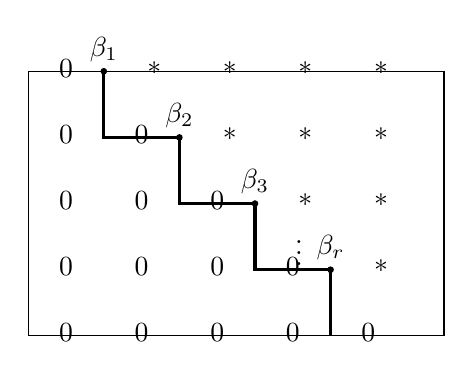
\begin{tikzpicture}[>=latex, scale=0.8]
  \draw (0,0) rectangle (6.6,-4.2);
  \draw[very thick] (1.2,0) -- (1.2,-1.05) -- (2.4,-1.05) -- (2.4,-2.1) -- (3.6,-2.1) -- (3.6,-3.15) -- (4.8,-3.15) -- (4.8,-4.2);
  \fill (1.2,0) circle (1.5pt) node[above]{$\beta_1$};
  \fill (2.4,-1.05) circle (1.5pt) node[above]{$\beta_2$};
  \fill (3.6,-2.1) circle (1.5pt) node[above]{$\beta_3$};
  \fill (4.8,-3.15) circle (1.5pt) node[above]{$\beta_r$};
  \node at (4.3,-2.75) {$\vdots$};
  \node at (0.6,0.05) {$0$};
  \node at (0.6,-1.0) {$0$};
  \node at (1.8,-1.0) {$0$};
  \node at (0.6,-2.05) {$0$};
  \node at (1.8,-2.05) {$0$};
  \node at (3.0,-2.05) {$0$};
  \node at (0.6,-3.1) {$0$};
  \node at (1.8,-3.1) {$0$};
  \node at (3.0,-3.1) {$0$};
  \node at (4.2,-3.1) {$0$};
  \node at (0.6,-4.15) {$0$};
  \node at (1.8,-4.15) {$0$};
  \node at (3.0,-4.15) {$0$};
  \node at (4.2,-4.15) {$0$};
  \node at (5.4,-4.15) {$0$};
  \node at (2.0,0.05) {$*$};
  \node at (3.2,0.05) {$*$};
  \node at (4.4,0.05) {$*$};
  \node at (5.6,0.05) {$*$};
  \node at (3.2,-1.0) {$*$};
  \node at (4.4,-1.0) {$*$};
  \node at (5.6,-1.0) {$*$};
  \node at (4.4,-2.05) {$*$};
  \node at (5.6,-2.05) {$*$};
  \node at (5.6,-3.1) {$*$};
\end{tikzpicture}
\end{center}
的矩阵, 其中在位置 $(1, j_1), \ldots, (r, j_r)$ 处有系数 $\beta_1, \ldots, \beta_r \in K^*$, 且 $j_1 < \cdots < j_r$.则 $B$ 的前 $r$ 行构成由 $A$ 的行向量在 $K^n$ 中生成的线性子空间的一个基.特别地有
\[
\operatorname{rg}_z A = \operatorname{rg}_z B = r\text{.}
\]
\end{bigtheorem}

\begin{proof}
设 $b_1, \ldots, b_m$ 是上面矩阵 $B$ 的行.我们首先证明 $b_1, \ldots, b_r$ 线性无关, 从而构成线性子空间
\[
\langle b_1, \ldots, b_r \rangle = \langle b_1, \ldots, b_m \rangle \subset K^n
\]
的一个基.如果我们能把 $A$ 借助初等行变换化为 $B$(这我们将在下面证明), 那么由定理~\mtref{thm:3.2.3}, 这个子空间恰是由 $A$ 的行向量在 $K^n$ 中生成的线性子空间.特别得到 $\operatorname{rg}_z A = \operatorname{rg}_z B = r$.

例如设 $\sum_{i = 1}^{r}\alpha_i b_i = 0$, 其中 $\alpha_i \in K$ 为某些系数.若记 $B = (\beta_{ij})_{i, j}$, 即 $\beta_{i, j_i} = \beta_i$ ($i = 1, \ldots, r$), 则得到方程组

\[
\begin{array}{r c l r c l r c l r c l}
\alpha_1\beta_1 & & & & & & & & & & & = 0, \\
\alpha_1\beta_{1, j_2} & + & \alpha_2\beta_2 & & & & & & & & & = 0, \\
\alpha_1\beta_{1, j_3} & + & \alpha_2\beta_{2, j_3} & + & \alpha_3\beta_3 & & & & & & & = 0, \\
& & \vdots & & & & & & & & & \\
\alpha_1\beta_{1, j_r} & + & \alpha_2\beta_{2, j_r} & + & \cdots & + & \alpha_r\beta_r & & & & & = 0,
\end{array}
\]

由它先得 $\alpha_1 = 0$, 然后 $\alpha_2 = 0$, 如此继续, 直到最终 $\alpha_r = 0$.于是 $b_1, \ldots, b_r$ 线性无关.

还剩下要证明: 每个矩阵 $A = (\alpha_{ij})_{i, j} \in K^{m \times n}$ 都能化为行阶梯形.为此按如下步骤进行.由于零矩阵已经是行阶梯形, 可以假设 $A \neq 0$.选取最小的指标 $j = j_1$, 使得存在 $i$ 满足 $\alpha_{ij} \neq 0$, 交换第一行与第 $i$ 行, 并令 $\beta_1 = \alpha_{i, j_1}$.通过 $m - 1$ 个保持第一行不变的类型 III 的变换, 可以使 $j_1$ 列中位于 $\beta_1$ 下方的所有元素都变为零.所得矩阵具有如下形状:

\[
\begin{pmatrix}
0 & \cdots & 0 & \beta_1 & * & \cdots & * \\
\hline
0 & \cdots & 0 & 0 & & \\
\vdots & & \vdots & \vdots & & A^{(1)} \\
0 & \cdots & 0 & 0 & &
\end{pmatrix}
\]

现在可以第二步把同一方法应用于 $A^{(1)}$ 以代替 $A$.把对 $A^{(1)}$ 所需的变换解释为整个矩阵的行变换, 并足够多次地重复这一方法, 就可用递归方式实现所断言的行阶梯形.若在某一步首次把 $A^{(r)}$ 化为零矩阵或空矩阵, 则构造终止.
\end{proof}

我们来看一个把矩阵化为行阶梯形的例子:

\[
\begin{pmatrix} 0 & 0 & 2 \\ 0 & 2 & 4 \\ 0 & 1 & 1 \end{pmatrix}
\longmapsto
\begin{pmatrix} 0 & 1 & 1 \\ 0 & 2 & 4 \\ 0 & 0 & 2 \end{pmatrix}
\longmapsto
\begin{pmatrix} 0 & 1 & 1 \\ 0 & 0 & 2 \\ 0 & 0 & 2 \end{pmatrix}
\longmapsto
\begin{pmatrix} 0 & 1 & 1 \\ 0 & 0 & 2 \\ 0 & 0 & 0 \end{pmatrix}
\]

高斯消元法尤其可以用来计算由给定向量生成的线性子空间 $U = \langle a_1, \ldots, a_m \rangle \subset K^n$ 的维数, 或给出 $U$ 的一个基.结合维数公式~\mtref{thm:1.6.5}, 还可以确定两个线性子空间 $U, U' \subset K^n$ 的交 $U \cap U'$ 的维数.进一步, 对线性映射 $f \colon K^n \longrightarrow K^m$, 自然可以确定像的一个基, 从而尤其确定秩 $\operatorname{rg} f$(此时把 $K^m$ 中的向量最好理解为行向量).再由维数公式~\mtref{thm:2.1.10} 还可以得到 $f$ 的核的维数.高斯消元法还适合给出 $\ker f$ 的一个基, 这一点我们将在 \ref{sec:3.5} 节关于线性方程组的部分看得更仔细.在解这些方程组时, 高斯方法导致未知量系统的逐步缩减, 直到最终得到一个其值可自由选取的剩余系统.于是某些未知量被去掉(消去), 所以"消元法"这个名称是说得通的.

与初等行变换相类似, 自然也可以定义矩阵的\emph{初等列变换}(\textup{elementare Spaltenumformungen})\index{chudengliebianhuan@初等列变换(elementare Spaltenumformungen)}.这样的变换可以解释为从右边乘以合适的初等矩阵, 并且像大定理~\mtref{bigthm:3.2.4} 那样可以证明, 每个矩阵都可以化为\emph{列阶梯形}(\textup{Spaltenstufenform})\index{liejietixing@列阶梯形(Spaltenstufenform)}.不过我们不必把所有细节都考虑一遍, 因为接下来我们要处理矩阵的转置.在这个过程下, 初等行变换变为初等列变换, 反之亦然.行阶梯形或列阶梯形的矩阵也如此.

\begin{definition}[\emph{转置矩阵}\index{zhuanzhijuzhen@转置矩阵(transponierte Matrix)}]\label{def:3.2.5}\index{zhuanzhijuzhen@转置矩阵(transponierte Matrix)}
设
\[
A = (\alpha_{ij})_{\substack{i = 1, \ldots, m\\ j = 1, \ldots, n}} \in K^{m \times n}\text{.}
\]
则
\[
A^t = (\alpha_{ij})_{\substack{j = 1, \ldots, n\\ i = 1, \ldots, m}} \in K^{n \times m}
\]
称为 $A$ 的转置矩阵.
\end{definition}

$A^t$ 的行由 $j = 1, \ldots, n$ 参数化, 列由 $i = 1, \ldots, m$ 参数化, 其中 $A^t$ 在位置 $(j, i)$, 即 $j$ 行与 $i$ 列的交点处, 具有系数 $\alpha_{ij}$, 它位于 $A$ 的位置 $(i, j)$ 处.换言之, $A^t$ 由 $A$ 交换行指标与列指标而得到.这相当于 $A$ 关于主对角线(即由位置 $(i, i)$, $i = 1, \ldots, \min(m, n)$ 组成的对角线)的反射.于是 $A$ 的行向量构成 $A^t$ 的列向量, 相应地 $A$ 的列向量构成 $A^t$ 的行向量.直接可见:

\begin{remark}\label{rem:3.2.6}
映射 $K^{m \times n} \longrightarrow K^{n \times m}$, $A \longmapsto A^t$, 是 $K$-向量空间的同构.特别地, 对 $A, B \in K^{m \times n}$, $\alpha \in K$ 有
\[
(A + B)^t = A^t + B^t, \qquad (\alpha A)^t = \alpha A^t\text{.}
\]
\end{remark}

\begin{remark}\label{rem:3.2.7}
对 $A \in K^{m \times n}$ 有
\[
(A^t)^t = A, \qquad \operatorname{rg}_z A = \operatorname{rg}_s A^t, \qquad \operatorname{rg}_s A = \operatorname{rg}_z A^t\text{.}
\]
\end{remark}

\begin{remark}\label{rem:3.2.8}
对可相乘的矩阵 $A, B$ 有
\[
(A \cdot B)^t = B^t \cdot A^t\text{.}
\]
\end{remark}

我们只给出注记~\mtref{rem:3.2.8} 的证明.对

\[
A = (\alpha_{ij})_{i, j} \in K^{m \times n}, \qquad B = (\beta_{jk})_{j, k} \in K^{n \times p}
\]

有

\[
\begin{array}{c}
(A \cdot B)^t = \left(\left(\sum_j \alpha_{ij}\beta_{jk}\right)_{i, k}\right)^t
= \left(\sum_j \alpha_{ij}\beta_{jk}\right)_{k, i} \\
= \left(\sum_j \beta_{jk}\alpha_{ij}\right)_{k, i} = B^t \cdot A^t,
\end{array}
\]

正如所断言的.

下面我们证明, 矩阵的转置对应线性映射的对偶.

\begin{theorem}\label{thm:3.2.9}
设 $f \colon V \longrightarrow W$ 是带 $V$ 的基 $X$ 与 $W$ 的基 $Y$ 的有限维 $K$-向量空间之间的线性映射.若 $X^*$(相应地 $Y^*$)是 $X$(相应地 $Y$)的对偶基, 而 $f^* \colon W^* \longrightarrow V^*$ 是 $f$ 的对偶线性映射, 则
\[
A_{f^*, Y^*, X^*} = (A_{f, X, Y})^t\text{.}
\]
\end{theorem}

\begin{proof}
设
\[
\begin{array}{c c}
X = (x_1, \ldots, x_n), & Y = (y_1, \ldots, y_m), \\
X^* = (x_1^*, \ldots, x_n^*), & Y^* = (y_1^*, \ldots, y_m^*),
\end{array}
\]
于是 $x_j^*(x_\nu) = \delta_{j\nu}$ 且 $y_i^*(y_\mu) = \delta_{i\mu}$.特别地, 对 $\varphi \in V^*$, 它关于基 $X^*$ 的唯一线性组合表示由
\[
\varphi = \sum_{j = 1}^{n}\varphi(x_j)x_j^*
\]
给出.这是定理~\mtref{thm:2.1.7} 的一个推论, 我们在定理~\mtref{thm:2.3.5} 的证明中已经看到.于是属于 $f^*$ 的矩阵可以如下描述:
\[
A_{f^*, Y^*, X^*} = \left(f^*(y_1^*)_{X^*}, \ldots, f^*(y_m^*)_{X^*}\right)
= \left(f^*(y_i^*)(x_j)\right)_{\substack{j = 1, \ldots, n\\ i = 1, \ldots, m}}\text{.}
\]
若 $f$ 的矩阵由
\[
A_{f, X, Y} = (\alpha_{ij})_{\substack{i = 1, \ldots, m\\ j = 1, \ldots, n}}, \qquad
\text{即} \qquad f(x_j) = \sum_{\mu = 1}^{m}\alpha_{\mu j}y_\mu
\]
给出, 则对 $i = 1, \ldots, m$ 得到
\[
\begin{array}{l}
f^*(y_i^*) = \sum_{j = 1}^{n}f^*(y_i^*)(x_j) \cdot x_j^* = \sum_{j = 1}^{n}(y_i^* \circ f)(x_j) \cdot x_j^* \\
\qquad = \sum_{j = 1}^{n}y_i^*\left(f(x_j)\right) \cdot x_j^* = \sum_{j = 1}^{n}y_i^*\left(\sum_{\mu = 1}^{m}\alpha_{\mu j}y_\mu\right) \cdot x_j^* \\
\qquad = \sum_{j = 1}^{n}\alpha_{ij} \cdot x_j^*,
\end{array}
\]
这意味着
\[
A_{f^*, Y^*, X^*} = (\alpha_{ij})_{\substack{j = 1, \ldots, n\\ i = 1, \ldots, m}} = (A_{f, X, Y})^t,
\]
正如所断言的.
\end{proof}

现在利用定理~\mtref{thm:2.3.7}, 即在定理~\mtref{thm:3.2.9} 的情形下映射 $f$ 与 $f^*$ 有相同的秩, 再由注记~\mtref{rem:3.2.2} 与注记~\mtref{rem:3.2.7} 得到

\[
\begin{array}{c}
\operatorname{rg}_s A_{f, X, Y} = \operatorname{rg} f = \operatorname{rg} f^* = \operatorname{rg}_s A_{f^*, Y^*, X^*} \\
= \operatorname{rg}_s (A_{f, X, Y})^t = \operatorname{rg}_z A_{f, X, Y}\text{.}
\end{array}
\]

由于矩阵总可以视为线性映射, 作为定理~\mtref{thm:3.2.9} 的推论得到:

\begin{corollary}\label{cor:3.2.10}
对矩阵 $A \in K^{m \times n}$ 有 $\operatorname{rg}_s A = \operatorname{rg}_z A$, 即列秩与行秩一致.
\end{corollary}

正如已经提到的, 从现在起我们将写 $\operatorname{rg} A$ 来代替 $\operatorname{rg}_s A$ 或 $\operatorname{rg}_z A$, 并把这个数称为矩阵 $A$ 的秩.矩阵的列秩与行秩一致是一个非平凡的结果, 我们在这里借助对偶映射的理论以简单的方式得到了它.但也可以换一种方式推出这个结果, 即利用: 当把矩阵 $A$ 从左边或右边乘以所谓可逆矩阵时, $A$ 的行秩与列秩不改变; 参见 \ref{sec:3.4} 节.

最后, 我们要利用推论~\mtref{cor:3.2.10} 说明, 在大定理~\mtref{bigthm:3.2.4} 中描述的矩阵化为行阶梯形的变换也可以在列向量的意义下解释.这尤其在人们想从给定向量组中选出一个极大线性无关子组时是有利的.

\begin{theorem}\label{thm:3.2.11}
设 $A = (a_1, \ldots, a_n) \in K^{m \times n}$ 是列向量为 $a_1, \ldots, a_n \in K^m$ 的矩阵, 它可以借助初等行变换化为行阶梯形 $B$, 其形状如大定理~\mtref{bigthm:3.2.4} 中所述, 其中对 $i = 1, \ldots, r$, 元素 $\beta_i \in K^*$ 分别位于指标为 $j_i$ 的列, 且 $1 \leq j_1 < \cdots < j_r \leq n$.则向量 $a_{j_1}, \ldots, a_{j_i}$ 线性无关, 并且当 $i \leq r$ 分别取为满足 $j_i \leq j$ 的最大值时, 有
\[
\langle a_1, \ldots, a_j \rangle = \langle a_{j_1}, \ldots, a_{j_i} \rangle, \qquad j = 1, \ldots, n\text{.}
\]
\end{theorem}

\begin{proof}
把矩阵 $A$ 通过删去指标 $j$ 不同于 $j_1, \ldots, j_r$ 的某些列,或删去对某个固定的 $j_0 \in \{1, \ldots, n\}$ 而言指标 $j \geq j_0$ 的所有列而缩小为矩阵 $A'$, 则通过对 $B$ 删去相应的列而缩小为矩阵 $B'$, 得到 $A'$ 的相应行阶梯形.于是
\[
\operatorname{rg}_z B' = \operatorname{rg}_z A' = \operatorname{rg}_s A',
\]
所以由 $A'$ 的列生成的线性子空间的维数恰好等于 $B'$ 的秩.特别地, 用这个论证得到系统 $a_{j_1}, \ldots, a_{j_r} \in K^m$ 的线性无关性, 再由推论~\mtref{cor:1.5.14} (ii) 得到所断言的线性子空间相等.
\end{proof}

\aufgaben

\noindent\textbf{习题 1.} 把矩阵
\[
A = \begin{pmatrix}
1 & 2 & 1 & 2 & 1 & 2 \\
2 & 5 & 4 & 5 & 4 & 5 \\
1 & 4 & 6 & 6 & 6 & 6 \\
2 & 5 & 6 & 9 & 7 & 11
\end{pmatrix} \in \mathbb{R}^{4 \times 6}
\]
化为行阶梯形.

\noindent\textbf{习题 2.} 计算矩阵
\[
A = \begin{pmatrix}
1 & 1 & 3 & 2 \\
1 & 1 & 2 & 3 \\
1 & 1 & 0 & 0
\end{pmatrix} \in K^{3 \times 4}
\]
的行秩, 分别对域 $K = \mathbb{Q}$ 与 $K = \mathbb{F}_5$; 其中 $\mathbb{F}_5$ 是 \ref{sec:1.3} 节习题 3 中含 5 个元素的域.(AT 318)

\noindent\textbf{习题 3.} 检验下列 $\mathbb{R}^5$ 中的向量组是否线性无关:
\[
(5, 4, 3, 2, 1), \quad (1, 2, 3, 4, 5), \quad (2, 2, 2, 2, 1), \quad (1, 0, 0, 1, 1), \quad (1, 0, 1, 0, 1)\text{.}
\]

\noindent\textbf{习题 4.} 设 $U \subset \mathbb{R}^4$ 是由向量
\[
(1, 2, 1, 2), \quad (2, 5, 4, 5), \quad (1, 4, 6, 6), \quad (2, 5, 6, 9), \quad (2, 6, 7, 8), \quad (1, 1, 0, 3)
\]
生成的线性子空间.计算 $\dim U$ 并给出 $U$ 的一个基.

\noindent\textbf{习题 5.} 在 $\mathbb{R}^5$ 中给定下列线性子空间:
\[
U = \left\langle (1, 0, 1, 0, 1), (2, 3, 4, 1, 2), (0, 3, 2, 1, 0) \right\rangle
\]
\[
U' = \left\langle (1, -1, 1, 0, 2), (1, 3, 3, 1, 1), (1, 2, 3, 1, 2) \right\rangle
\]
计算 $\dim U$ 与 $\dim U'$, 并证明 $U \subset U'$.(AT 319)

\noindent\textbf{习题 6.} 在 $\mathbb{R}^6$ 中考察线性子空间
\[
U = \left\langle (1, 1, 1, 0, 1, 1), (2, 3, 4, 0, 2, 1), (0, 3, 2, 1, 1, 1) \right\rangle,
\]
\[
U' = \left\langle (2, 6, 6, 2, 2, 1), (0, 9, 4, 3, 0, 1), (1, 2, 3, 1, 2, 1) \right\rangle,
\]
并计算 $\dim(U \cap U')$.

\noindent\textbf{习题 7.} 考察线性形式
\[
\begin{array}{l l}
f_1 \colon \mathbb{R}^5 \longrightarrow \mathbb{R}, & (\alpha_1, \ldots, \alpha_5) \longmapsto (\alpha_2 + \alpha_3 + \alpha_4 + \alpha_5), \\
f_2 \colon \mathbb{R}^5 \longrightarrow \mathbb{R}, & (\alpha_1, \ldots, \alpha_5) \longmapsto (\alpha_1 + 2\alpha_2 - \alpha_3 - \alpha_4), \\
f_3 \colon \mathbb{R}^5 \longrightarrow \mathbb{R}, & (\alpha_1, \ldots, \alpha_5) \longmapsto (5\alpha_1 + 2\alpha_2 - \alpha_3 + 2\alpha_4 - 2\alpha_5), \\
f_4 \colon \mathbb{R}^5 \longrightarrow \mathbb{R}, & (\alpha_1, \ldots, \alpha_5) \longmapsto (\alpha_1 - \alpha_2 + \alpha_4 - \alpha_5),
\end{array}
\]
并检验它们是否在对偶空间 $(\mathbb{R}^5)^*$ 中构成线性无关组.

\noindent\textbf{习题 8.} 线性形式 $f_1, f_2, f_3, f_4$ 如习题 7 中所给.对 $\mathbb{R}$-线性映射
\[
f \colon \mathbb{R}^5 \longrightarrow \mathbb{R}^4, \quad x \longmapsto \left(f_1(x), f_2(x), f_3(x), f_4(x)\right),
\]
确定 $\dim_\mathbb{R} \ker f$ 与 $\dim_\mathbb{R} \operatorname{im} f$.再给出 $\operatorname{im} f$ 的一个基.

\noindent\textbf{习题 9.} 设 $\mathbb{F}_2$ 是含 2 个元素的域.在 $\mathbb{F}_2$-向量空间 $\mathbb{F}_2^{2000}$ 中, 由
\[
v_i = \begin{cases}
0, & \text{若 } i \text{ 不被 } 4 \text{ 整除}, \\
(1 + \delta_{ij})_{j = 1, \ldots, 2000}, & \text{若 } i \text{ 被 } 4, \text{ 不被 } 8 \text{ 整除}, \\
(1 + \delta_{i - 1, j} + \delta_{i + 1, j})_{j = 1, \ldots, 2000}, & \text{若 } i \text{ 被 } 8 \text{ 整除}
\end{cases}
\]
定义一族向量 $(v_i)_{i = 1, \ldots}$.考察由诸 $v_i$ 生成的线性子空间 $U \subset \mathbb{F}_2^{2000}$, 确定 $\dim_{\mathbb{F}_2} U$ 并给出 $U$ 的一个基.(AT 320)

\section{矩阵环与可逆矩阵}\index{juzhenhuan@矩阵环(Matrizenring)}\index{kenijuzhen@可逆矩阵(invertierbare Matrix)}\index{huan@环(Ring)}\label{sec:3.3}

对 $n \in \mathbb{N}$, 在所有 $(n \times n)$-矩阵的集合 $K^{n \times n}$ 上, 与域的情形相类似, 除加法外还有乘法, 不过对 $n \geq 2$ 它不交换.此时形如

\[
\begin{pmatrix} 1 & 0 \\ 0 & 0 \end{pmatrix} \cdot \begin{pmatrix} 0 & 0 \\ 1 & 0 \end{pmatrix} = 0
\]

的等式表明, 对 $n \geq 2$, $K^{n \times n}$ 中存在非平凡\emph{零因子}(\textup{Nullteiler})\index{lingyinzi@零因子(Nullteiler)}.矩阵 $A \in K^{n \times n}$ 称为零因子, 如果存在非零矩阵 $B \in K^{n \times n}$ 使得 $A \cdot B = 0$ 或 $B \cdot A = 0$.

\begin{definition}[\emph{环}\index{huan@环(Ring)}]\label{def:3.3.1}\index{huan@环(Ring)}
带两个运算 $+$ (加法)与 $\cdot$ (乘法)的集合 $R$ 称为环, 如果下列条件成立:
\begin{enumerate}
\item[(i)] $R$ 关于加法是阿贝尔群.
\item[(ii)] 乘法是结合的, 即对 $a, b, c \in R$ 有
\[
(a \cdot b) \cdot c = a \cdot (b \cdot c)\text{.}
\]
\item[(iii)] 加法与乘法满足分配律, 即对 $a, b, c \in R$ 有
\[
a \cdot (b + c) = a \cdot b + a \cdot c, \qquad (a + b) \cdot c = a \cdot c + b \cdot c\text{.}
\]
\end{enumerate}
关于加法的中性元 $0$ 称为 $R$ 的零元.环 $R$ 称为交换的, 如果乘法是交换的.此外, 元素 $e \in R$ 称为单位元, 如果对一切 $a \in R$ 有 $e \cdot a = a = a \cdot e$; 此时也写 $1$ 来代替 $e$.
\end{definition}

环的单位元(若存在)自然唯一确定.环的最简单例子是\emph{零环}(\textup{Nullring})\index{linghuan@零环(Nullring)} $0$.它只由一个元素 $0$ 组成, 带运算 $0 + 0 = 0$ 与 $0 \cdot 0 = 0$; 于是这里 $0$ 既是零元又是单位元.但我们还要给出一些更有意思的例子.

\begin{enumerate}
\item 整数环 $\mathbb{Z}$ 在通常的加法与乘法下是带单位元的\emph{交换环}(\textup{kommutativer Ring mit Eins})\index{jiaohuanhuan@交换环(kommutativer Ring mit Eins)}.
\item 每个域, 例如 $\mathbb{Q}, \mathbb{R}$ 或 $\mathbb{C}$, 都是带单位元的交换环.
\item 设 $V$ 是 $K$-向量空间, $R = \operatorname{Hom}_K(V, V)$ 是 $V$ 的自同态的 $K$-向量空间.若在 $R$ 中把线性映射的通常加法作为加法,把线性映射的复合作为乘法, 则 $R$ 是一个环, 即所谓 $V$ 的\emph{自同态环}(\textup{Endomorphismenring; End$_K$(V)})\index{zitongtaihuan@自同态环(Endomorphismenring; End$_K$(V))}.这个环记作 $\operatorname{End}_K(V)$.它以零映射 $0 \colon V \longrightarrow V$ 为零元, 以恒等映射 $\mathrm{id} \colon V \longrightarrow V$ 为单位元.可以想到, 对 $\dim_K V \geq 2$, $\operatorname{End}_K(V)$ 不交换.
\item 对 $n \in \mathbb{N}$, $n$ 阶方阵的 $K$-向量空间 $K^{n \times n}$ 在 \ref{sec:3.1} 节引入的矩阵加法与乘法下是一个环.其中 $K^{0 \times 0}$ 是零环, $K^{1 \times 1}$ 是一个环, 我们把它按自然方式与域 $K$ 等同.此外, 对 $n \geq 2$, $K^{n \times n}$ 中的乘法不再交换.矩阵 $E = (\delta_{ij})_{i, j} \in K^{n \times n}$, 常也记作 $1$, 是 $K^{n \times n}$ 中的单位元, 称为 $n$ 阶单位矩阵.正如我们开头看到的, 对 $n \geq 2$, $K^{n \times n}$ 含非平凡零因子.
\end{enumerate}

例 (3) 与 (4) 借助 \ref{sec:3.1} 节的结果可以看出是相关的.更确切地有:

\begin{theorem}\label{thm:3.3.2}
设 $V$ 是 $K$-向量空间, $X = (x_1, \ldots, x_n)$ 是 $V$ 的基.则映射
\[
\varPsi \colon \operatorname{End}_K(V) \longrightarrow K^{n \times n}, \qquad f \longmapsto A_{f, X, X},
\]
是环的同构, 即满足
\[
\varPsi(f + g) = \varPsi(f) + \varPsi(g), \qquad \varPsi(f \circ g) = \varPsi(f) \cdot \varPsi(g)
\]
的双射, 对一切元素 $f, g \in \operatorname{End}_K(V)$ 成立.
\end{theorem}

\begin{proof}
由定理~\mtref{thm:3.1.4}, $\varPsi$ 是与加法相容的双射.与乘法的相容性由定理~\mtref{thm:3.1.9} 推出.
\end{proof}

若 $a$ 是带单位元的环 $R$ 的元素, 则元素 $b \in R$ 称为 $a$ 的逆, 如果 $a \cdot b = 1 = b \cdot a$.$a \in R$ 的逆元素(若存在)总是唯一确定的.事实上, 若两个元素 $b, b' \in R$ 都是 $a$ 的逆, 或更准确地说, $b$ 是 $a$ 的逆而仅成立 $a \cdot b' = 1$(或相应地 $b' \cdot a = 1$), 则
\[
b = b \cdot 1 = b \cdot (a \cdot b') = (b \cdot a) \cdot b' = 1 \cdot b' = b',
\]
或相应地
\[
b = 1 \cdot b = (b' \cdot a) \cdot b = b' \cdot (a \cdot b) = b' \cdot 1 = b'\text{.}
\]
$a$ 的逆元素记作 $a^{-1}$, 此时称 $a$ 可逆或称为单位.在域中, 每个元素 $a \neq 0$ 都是单位.另一方面, 在\emph{矩阵环}(\textup{Matrizenring})\index{juzhenhuan@矩阵环(Matrizenring)} $K^{n \times n}$ 中对 $n \geq 2$ 恒有非平凡零因子, 这样的矩阵不可能是单位.事实上, 若 $A \in K^{n \times n}$ 是单位, 而 $B \in K^{n \times n}$ 是满足 $A \cdot B = 0$ 的矩阵, 则用 $A$ 的\emph{逆矩阵}(\textup{inverse Matrix})\index{nijuzhen@逆矩阵(inverse Matrix)} $A^{-1}$ 必得 $B = A^{-1} \cdot A \cdot B = 0$.

\begin{remark}\label{rem:3.3.3}
在带单位元的环 $R$ 中, 一切单位的集合 $R^*$ 关于乘法构成一个群.
\end{remark}

这个断言直接由环或单位的定义性质得出.

\begin{remark}\label{rem:3.3.4}
设 $V$ 是 $K$-向量空间, $f \in \operatorname{End}_K(V)$.则下列条件等价:
\begin{enumerate}
\item[(i)] 存在元素 $g \in \operatorname{End}_K(V)$ 使得 $f \circ g = \mathrm{id}_V = g \circ f$, 即 $f$ 是 $\operatorname{End}_K(V)$ 中的单位;
\item[(ii)] $f$ 是 $V$ 的自同构.
\end{enumerate}
\end{remark}

\begin{proof}
关系 $f \circ g = \mathrm{id}_V$ 蕴含 $f$ 满射, 相应地 $g \circ f = \mathrm{id}_V$ 蕴含 $f$ 单射.于是由条件 (i) 得 (ii); 反过来, 从 (ii) 也推出 (i), 只要把 $g$ 取为 $f$ 的逆映射.
\end{proof}

自同态环 $\operatorname{End}_K(V)$ 的\emph{单位群}(\textup{Einheitengruppe; R*})\index{danweiqun@单位群(Einheitengruppe; R*)}因此恰好由 $V$ 的一切自同构组成.我们把这个群记作 $\operatorname{Aut}_K(V)$, 称之为 $V$ 的\emph{自同构群}(\textup{Automorphismengruppe; Aut$_K$(V)})\index{zitonggouqun@自同构群(Automorphismengruppe; Aut$_K$(V))}.矩阵环 $K^{n \times n}$ 的单位群记作 $\mathrm{Gl}(n, K)$, 称之为\emph{一般线性群}(\textup{allgemeine lineare Gruppe; Gl(n,K)})\index{yibanxianxingqun@一般线性群(allgemeine lineare Gruppe; Gl(n,K))} (general linear group).$\mathrm{Gl}(n, K)$ 的元素称为可逆(或可逆的, 或正则的, 或非奇异的, 或\emph{非退化}(\textup{nicht ausgeartet})\index{feituihua@非退化(nicht ausgeartet)}的)矩阵.

\begin{theorem}\label{thm:3.3.5}
设 $V$ 是 $K$-向量空间, $X = (x_1, \ldots, x_n)$ 是 $V$ 的基.则定理~\mtref{thm:3.3.2} 中的同构
\[
\varPsi \colon \operatorname{End}_K(V) \xrightarrow{\sim} K^{n \times n}, \qquad f \longmapsto A_{f, X, X},
\]
在相应单位群之间限制为同构
\[
\operatorname{Aut}_K(V) \xrightarrow{\sim} \mathrm{Gl}(n, K),
\]
即限制为尊重各自群结构的双射.
\end{theorem}

\begin{proof}
$\varPsi$ 把恒等映射 $\mathrm{id}_V \in \operatorname{End}_K(V)$ 映到单位矩阵 $E \in K^{n \times n}$, 即把 $\operatorname{End}_K(V)$ 的单位元映到 $K^{n \times n}$ 的单位元.由此直接推出 $\varPsi$ 把单位映到单位.由于逆映射 $\varPsi^{-1}$ 具有相应的性质, 断言得证.
\end{proof}

我们要把定理的内容在稍一般的框架中表述出来.

\begin{theorem}\label{thm:3.3.6}
设 $f \colon V \longrightarrow W$ 是带基 $X = (x_1, \ldots, x_n)$ 与 $Y = (y_1, \ldots, y_n)$ 的向量空间之间的 $K$-线性映射.描述矩阵 $A = A_{f, X, Y}$ 可逆, 当且仅当 $f$ 是同构.
\end{theorem}

\begin{proof}
像注记~\mtref{rem:3.3.4} 的证明那样考虑可知, $f$ 双射, 当且仅当存在 $K$-线性映射 $g \colon W \longrightarrow V$ 使得 $f \circ g = \mathrm{id}_W$ 且 $g \circ f = \mathrm{id}_V$.后者由定理~\mtref{thm:3.1.4} 与定理~\mtref{thm:3.1.9} 等价于存在矩阵 $B \in K^{n \times n}$ 使得 $A_{f, X, Y} \cdot B = 1$ 且 $B \cdot A_{f, X, Y} = 1$.
\end{proof}

\begin{corollary}\label{cor:3.3.7}
对矩阵 $A \in K^{n \times n}$, 下列条件等价:
\begin{enumerate}
\item[(i)] $A$ 可逆;
\item[(ii)] 存在矩阵 $B \in K^{n \times n}$ 使得 $B \cdot A = 1$;
\item[(iii)] 存在矩阵 $B \in K^{n \times n}$ 使得 $A \cdot B = 1$;
\item[(iv)] $\operatorname{rg} A = n$.
\end{enumerate}
\end{corollary}

\begin{proof}
把 $A$ 实现为线性映射, 例如实现为映射
\[
f \colon K^n \longrightarrow K^n, \qquad x \longmapsto A \cdot x\text{.}
\]
则关于 $K^n$ 上的标准基, $A$ 就是属于 $f$ 的矩阵.利用定理~\mtref{thm:3.3.5} 与注记~\mtref{rem:3.2.2}, 只需证明下列条件等价:

(i$'$) $f$ 是自同构;

(ii$'$) 存在 $K$-线性映射 $g \colon K^n \longrightarrow K^n$ 使得 $g \circ f = \mathrm{id}$;

(iii$'$) 存在 $K$-线性映射 $g \colon K^n \longrightarrow K^n$ 使得 $f \circ g = \mathrm{id}$;

(iv$'$) $\operatorname{rg} f = n$.

若 $f$ 是自同构, 则条件 (ii$'$), (iii$'$) 与 (iv$'$) 自然成立.反过来, 若 (ii$'$) 成立, 则 $f$ 单射, 由推论~\mtref{cor:2.1.11} 是自同构.在条件 (iii$'$) 或 (iv$'$) 下, $f$ 满射, 从而同样由推论~\mtref{cor:2.1.11} 是自同构.
\end{proof}

推论~\mtref{cor:3.3.7} 的条件 (iv) 给出了检验矩阵 $A \in K^{n \times n}$ 可逆性的有用判据, 这尤其是因为我们可以借助初等行变换明确地确定矩阵的秩; 参见大定理~\mtref{bigthm:3.2.4}.例如可见, 对 $i, j \in \{1, \ldots, n\}$, $i \neq j$ 与 $\alpha \in K^*$, 初等矩阵

\[
E + (\alpha - 1)E_{ii}, \qquad E + \alpha E_{ij}, \qquad E - E_{ii} - E_{jj} + E_{ij} + E_{ji}
\]

在 $K^{n \times n}$ 中可逆; 这里 $E$ 如 \ref{sec:3.2} 节那样是 $K^{n \times n}$ 中的单位矩阵, 而 $E_{ij} = (\delta_{i\mu}\delta_{j\nu})_{\mu, \nu}$.初等矩阵由单位矩阵 $E$ 经初等行变换得到, 因此与后者有相同的秩, 即 $n$; 参见定理~\mtref{thm:3.2.3}.下面我们还要明确确定上述初等矩阵的逆(它们(顺便说)很容易"猜"出来).

我们可以利用刚才的论证把 \ref{sec:3.2} 节处理的高斯消元法推广到矩阵求逆.例如从矩阵 $A \in K^{n \times n}$ 出发, 按大定理~\mtref{bigthm:3.2.4} 用初等行变换把 $A$ 化为行阶梯形 $B$.现在假设 $A$ 可逆, 则由推论~\mtref{cor:3.3.7} 有 $\operatorname{rg} A = \operatorname{rg} B = n$, 并且在大定理~\mtref{bigthm:3.2.4} 的情形下, 元素 $\beta_1, \ldots, \beta_n$ 恰好位于主对角线上, 即:

\[
B = \begin{pmatrix}
\beta_1 & * & \cdots & * \\
0 & \beta_2 & \cdots & * \\
\vdots & \ddots & \ddots & \vdots \\
0 & \cdots & 0 & \beta_n
\end{pmatrix}\text{.}
\]

通过用 $\beta_i^{-1}$, $i = 1, \ldots, n$ 乘第 $i$ 行, 可以假设所有 $\beta_i$ 都取值为 $1$.然后从其余各行减去第 $n$ 行的倍数, 以这种方式使第 $n$ 列中位于 $\beta_n$ 上方的所有元素都变为零.相应地处理其余各列, 于是得到: 在可逆的情形, $A$ 可借助初等行变换化为单位矩阵 $E$.如 \ref{sec:3.2} 节所见, 每个这样的行变换都可以解释为从左边乘以某个初等矩阵.因此我们找到初等矩阵 $S_1, \ldots, S_r \in K^{n \times n}$ 使得

\[
S_r \cdot \ldots \cdot S_1 \cdot A = E,
\]

从右边乘以 $A^{-1}$ 得到 $A^{-1} = S_r \cdot \ldots \cdot S_1$.把

\[
A^{-1} = S_r \cdot \ldots \cdot S_1 \cdot E
\]

写出来, 我们看到: 把 $A$ 化为单位矩阵 $E$ 的那些初等行变换, 也把 $E$ 本身化为矩阵 $A^{-1}$!

因此矩阵求逆的方法可以描述如下: 用一串初等行变换把 $A$ 化为行阶梯形, 并在每一步也对单位矩阵施行相应的行变换.然后若从行阶梯形读出 $\operatorname{rg} A = n$, 则 $A$ 可逆, 于是继续施行变换, 直到把 $A$ 化为单位矩阵.由单位矩阵经相应变换得到的矩阵就是 $A$ 的逆矩阵 $A^{-1}$.例如用这个方法对 $\alpha \in K$, $i \neq j$ 看出:

\[
\begin{array}{r}
\left(E + (\alpha - 1)E_{ii}\right)^{-1} = E + (\alpha^{-1} - 1)E_{ii}, \\
(E + \alpha E_{ij})^{-1} = E - \alpha E_{ij}, \\
(E - E_{ii} - E_{jj} + E_{ij} + E_{ji})^{-1} = E - E_{ii} - E_{jj} + E_{ij} + E_{ji}\text{.}
\end{array}
\]

作为这个方法的一个副产品, 我们还可以记下:

\begin{theorem}\label{thm:3.3.8}
每个可逆矩阵 $A \in \mathrm{Gl}(n, K)$ 都是类型
\[
\begin{array}{c c}
E + (\alpha - 1)E_{ii}, & \alpha \in K^*, \\
E + E_{ij}, & i \neq j,
\end{array}
\]
($1 \leq i, j \leq n$) 的初等矩阵的乘积.其中 $E \in K^{n \times n}$ 是单位矩阵, $E_{ij} = (\delta_{\mu i}\delta_{\nu j})_{\mu, \nu}$.
\end{theorem}

\begin{proof}
我们刚刚看到, $A$ 可以借助 \ref{sec:3.2} 节中类型 I--IV 的初等行变换化为单位矩阵, 而 $A^{-1}$ 是相应初等矩阵的乘积.但类型 III 的初等行变换, 即对 $\alpha \in K^*$ 与某些指标 $i \neq j$ 把第 $j$ 行的 $\alpha$ 倍加到第 $i$ 行, 也可以解释为类型 I 与 II 的初等行变换的一串: 把第 $j$ 行乘以 $\alpha$, 把它加到第 $i$ 行, 然后又把第 $j$ 行乘以 $\alpha^{-1}$.相应地, 类型 IV 的初等行变换, 即对某些指标 $i \neq j$ 交换第 $i$ 行与第 $j$ 行, 也可以解释为类型 I 与 II 的变换的一串: 把第 $j$ 行加到第 $i$ 行, 把第 $j$ 行乘以 $1$, 把第 $i$ 行加到第 $j$ 行, 最后从第 $i$ 行减去第 $j$ 行.其中最后一步是类型 III 的变换, 因此可以分解为类型 I 与 II 的变换的一串.

把上面的论证应用于 $A^{-1}$ 以代替 $A$, 我们看到 $A$ 正如所断言的是与类型 I 和 II 的初等行变换相对应的初等矩阵的乘积.
\end{proof}

若想明确给出给定矩阵 $A \in \mathrm{Gl}(n, K)$ 的初等矩阵分解, 最好按如下步骤进行: 用初等行变换把 $A$ 化为单位矩阵, 从而得到形如 $A^{-1} = S_r \cdot \ldots \cdot S_1$ 的分解, 其中 $S_1, \ldots, S_r$ 是初等矩阵.取逆给出 $A = S_1^{-1} \cdot \ldots \cdot S_r^{-1}$, 其中如上所述, 各 $S_i^{-1}$ 又都是初等矩阵.若想限于定理~\mtref{thm:3.3.8} 中提到的初等矩阵, 则必要时还要把 $S_i^{-1}$ 进一步分解.

\aufgaben

\noindent\textbf{习题 1.} 设 $X$ 是一个集合, $R$ 是带 $1$ 的环.证明: 一切映射 $X \longrightarrow R$ 的集合 $\operatorname{Abb}(X, R)$ 在 $R$ 值函数的通常加法与乘法下构成一个环.描述这个环的单位群.

\noindent\textbf{习题 2.} 给出一个 $K$-向量空间 $V$, 对它存在非单位 $f, g \in \operatorname{End}_K(V)$ 使得 $f \circ g = \mathrm{id}_V$.

\noindent\textbf{习题 3.} 设 $f \colon U \longrightarrow U$ 是有限维 $K$-向量空间的自同态.则下列条件等价: (AT 321)
\begin{enumerate}
\item[(i)] $\operatorname{rg} f < \dim_K U$;
\item[(ii)] $f$ 是 $\operatorname{End}_K(V)$ 中的左零因子, 即存在 $g \in \operatorname{End}_K(V)$, $g \neq 0$, 使得 $f \circ g = 0$;
\item[(iii)] $f$ 是 $\operatorname{End}(V)$ 中的右零因子, 即存在 $g \in \operatorname{End}_K(V)$, $g \neq 0$, 使得 $g \circ f = 0$.
\end{enumerate}
特别地, $\operatorname{End}_K(V)$ 中的左零因子也是右零因子, 反之亦然.在矩阵环 $K^{n \times n}$ 中相应的结论也成立.

\noindent\textbf{习题 4.} 检验下列矩阵的可逆性, 并在可能时给出逆矩阵:
\[
\begin{pmatrix}
1 & 2 & 3 & 2 & 4 \\
1 & 1 & 2 & 2 & 4 \\
1 & 3 & 4 & 3 & 7 \\
2 & 3 & 5 & 3 & 8 \\
0 & 0 & 1 & 0 & 1
\end{pmatrix},
\quad
\begin{pmatrix}
1 & 1 & 1 & 2 & 0 \\
1 & 0 & 2 & 1 & 0 \\
1 & 1 & 1 & 2 & 1 \\
0 & 1 & 2 & 1 & 0 \\
1 & 1 & 1 & 2 & 0
\end{pmatrix} \in \mathbb{R}^{5 \times 5}
\]

\noindent\textbf{习题 5.} 在可能的情况下, 把下列矩阵写为初等矩阵的乘积:
\[
\begin{pmatrix}
1 & 0 & 0 & 1 \\
1 & 1 & 0 & 3 \\
1 & 1 & 1 & 4 \\
1 & 0 & 1 & 2
\end{pmatrix},
\quad
\begin{pmatrix}
1 & 1 & 1 & 1 \\
0 & 1 & 1 & 1 \\
0 & 0 & 1 & 1 \\
0 & 0 & 0 & 1
\end{pmatrix} \quad \in \mathbb{R}^{4 \times 4}
\]

\noindent\textbf{习题 6.} 对 $A \in \mathrm{Gl}(n, K)$ 证明 $(A^{-1})^t = (A^t)^{-1}$.

\noindent\textbf{习题 7.} 对 $m, r, s \in \mathbb{N} - \{0\}$ 考察矩阵
\[
A \in K^{m \times m}, \qquad B \in K^{m \times s}, \qquad C \in K^{r \times m}, \qquad D \in K^{r \times s},
\]
满足
\[
\operatorname{rg} \begin{pmatrix} A & B \\ C & D \end{pmatrix} = m,
\]
其中 $A$ 可逆.证明 $D = C \cdot A^{-1}B$.(AT 323)

\section{基变换}\index{jibianhuan@基变换(Basiswechsel)}\label{sec:3.4}

我们看到, 向量空间之间的 $K$-线性映射在固定基之后可以用矩阵描述.本节尤其要研究: 当过渡到其他基时, 描述矩阵如何改变.我们以基的一个刻画开始.

\begin{remark}\label{rem:3.4.1}
设 $V$ 是带基 $X = (x_1, \ldots, x_n)$ 的 $K$-向量空间.对带系数 $\alpha_{ij} \in K$ 的 $n$ 个元素 $y_j = \sum_{i = 1}^{n}\alpha_{ij}x_i \in V$, $j = 1, \ldots, n$, 考察矩阵 $A = (\alpha_{ij})_{i, j} \in K^{n \times n}$, 即由 $x_j \longmapsto y_j$ 定义的 $K$-线性映射 $f \colon V \longrightarrow V$ 的矩阵 $A_{f, X, X}$.则下列条件等价:
\begin{enumerate}
\item[(i)] $Y = (y_1, \ldots, y_n)$ 是 $V$ 的基;
\item[(ii)] $\operatorname{rg} A = n$;
\item[(iii)] $A \in \mathrm{Gl}(n, K)$, 即 $A$ 可逆.
\end{enumerate}
\end{remark}

\begin{proof}
若 $Y$ 是 $V$ 的基, 则 $f$ 是同构, 由注记~\mtref{rem:3.2.2} 得 $\operatorname{rg} A = \operatorname{rg} f = \dim_K V = n$.若再有 $\operatorname{rg} A = n$, 则由推论~\mtref{cor:3.3.7} 有 $A \in \mathrm{Gl}(n, K)$.由后一条件又由定理~\mtref{thm:3.3.6} 得 $f$ 是同构, 从而 $Y$ 是基.
\end{proof}

若在注记~\mtref{rem:3.4.1} 的情形下 $Y$ 是 $V$ 的基, 则称 $A = (\alpha_{ij})_{i, j}$ 为\emph{基变换的矩阵}(\textup{Matrix eines Basiswechsels})\index{jibianhuandejuzhen@基变换的矩阵(Matrix eines Basiswechsels)}.这时也可以把 $A$ 解释为恒等映射 $\mathrm{id} \colon V \longrightarrow V$ 关于基 $Y$ 与 $X$ 的矩阵, 即 $A = A_{\mathrm{id}, Y, X}$, 我们为了精确说明基变换的方式将总是这样处理.特别地, 由注记~\mtref{rem:3.4.1} 得到, 在固定 $V$ 的基 $X$ 的情形下, 每个矩阵 $A \in \mathrm{Gl}(n, K)$ 都可以解释为某个合适的基 $Y$ 的形式为 $A_{\mathrm{id}, Y, X}$ 的基变换矩阵.由方程

\[
A_{\mathrm{id}, Y, X} \cdot A_{\mathrm{id}, X, Y} = A_{\mathrm{id}, X, X} = 1,
\]

参见定理~\mtref{thm:3.1.9}, 我们读出:

\begin{remark}\label{rem:3.4.2}
设 $V$ 是带有限基 $X$ 与 $Y$ 的 $K$-向量空间.则基变换矩阵 $A_{\mathrm{id}, Y, X}$ 可逆, 它的逆由基变换矩阵 $A_{\mathrm{id}, X, Y}$ 给出.
\end{remark}

进一步由定理~\mtref{thm:3.1.7} 得到:

\begin{remark}\label{rem:3.4.3}
设 $V$ 是带有限基 $X$ 与 $Y$ 的 $K$-向量空间.对 $a \in V$, 用 $a_X$ 或 $a_Y$ 分别表示 $a$ 关于 $X$ 或 $Y$ 的坐标列向量.则
\[
a_X = A_{\mathrm{id}, Y, X} \cdot a_Y, \qquad a_Y = A_{\mathrm{id}, X, Y} \cdot a_X\text{.}
\]
\end{remark}

接下来要研究线性映射的描述矩阵在基变换下如何变化.

\begin{theorem}\label{thm:3.4.4}
设 $f \colon V \longrightarrow W$ 是有限维 $K$-向量空间之间的 $K$-线性映射.若 $X, X'$ 是 $V$ 的基, $Y, Y'$ 是 $W$ 的基, 则
\[
A_{f, X', Y'} = (A_{\mathrm{id}, Y', Y})^{-1} \cdot A_{f, X, Y} \cdot A_{\mathrm{id}, X', X}\text{.}
\]
\end{theorem}

\begin{proof}
把定理~\mtref{thm:3.1.9} 应用于 $f = \mathrm{id}_W \circ f \circ \mathrm{id}_V$, 得到
\[
A_{f, X', Y'} = A_{\mathrm{id}, Y, Y'} \cdot A_{f, X, Y} \cdot A_{\mathrm{id}, X', X},
\]
其中 $A_{\mathrm{id}, Y, Y'} = (A_{\mathrm{id}, Y', Y})^{-1}$.
\end{proof}

\begin{corollary}\label{cor:3.4.5}
设 $f \colon V \longrightarrow V$ 是带基 $X, X'$ 的有限维 $K$-向量空间 $V$ 的自同态.则
\[
A_{f, X', X'} = (A_{\mathrm{id}, X', X})^{-1} \cdot A_{f, X, X} \cdot A_{\mathrm{id}, X', X}\text{.}
\]
\end{corollary}

现在我们还要给出关于矩阵秩的一些应用.

\begin{theorem}\label{thm:3.4.6}
对矩阵 $S \in \mathrm{Gl}(m, K)$, $A \in K^{m \times n}$ 与 $T \in \mathrm{Gl}(n, K)$ 有
\[
\operatorname{rg}(S \cdot A \cdot T) = \operatorname{rg} A\text{.}
\]
\end{theorem}

\begin{proof}
考察线性映射 $f \colon K^n \longrightarrow K^m$, $a \longmapsto A \cdot a$.若在 $K^n$ 与 $K^m$ 中分别采用标准基, 则 $A$ 就是属于 $f$ 的矩阵.再把 $S^{-1}$ 解释为 $K^m$ 中的基变换矩阵, 把 $T$ 解释为 $K^n$ 中的基变换矩阵, 则由注记~\mtref{rem:3.2.2} 与定理~\mtref{thm:3.4.4} 得
\[
\operatorname{rg}(S \cdot A \cdot T) = \operatorname{rg} f = \operatorname{rg} A\text{.}
\]
\end{proof}

\begin{lemma}\label{lem:3.4.7}
设 $f \colon V \longrightarrow W$ 是向量空间之间的 $K$-线性映射, 其中 $\dim_K V = n$, $\dim_K W = m$.设 $r = \operatorname{rg} f$.则存在 $V$ 的基 $X = (x_1, \ldots, x_n)$ 与 $W$ 的基 $Y = (y_1, \ldots, y_m)$, 使得
\[
A_{f, X, Y} = \begin{pmatrix} E_r & 0 \\ 0 & 0 \end{pmatrix},
\]
其中 $E_r$ 是 $(r \times r)$-单位矩阵, 而 $0$ 各表示合适的(也可能为空)系数全为 $0$ 的区域.
\end{lemma}

\begin{proof}
选取 $\operatorname{im} f$ 的基 $y_1, \ldots, y_r$, 并把它扩充为 $W$ 的基 $Y = (y_1, \ldots, y_m)$.再设 $x_1, \ldots, x_r$ 分别是 $y_1, \ldots, y_r$ 在 $f$ 下的原像.由注记~\mtref{rem:2.1.5} 它们线性无关, 并且如定理~\mtref{thm:2.1.10} 的证明中所证明的, 可以用元素 $x_{r + 1}, \ldots, x_n \in \ker f$ 把它们扩充为 $V$ 的基 $X$.于是
\[
f(x_j) = \begin{cases}
y_j, & \text{对 } j = 1, \ldots, r, \\
0, & \text{对 } j = r + 1, \ldots, n,
\end{cases}
\]
从而 $A_{f, X, Y}$ 具有所求的形式.
\end{proof}

\begin{theorem}\label{thm:3.4.8}
设 $A \in K^{m \times n}$ 且 $\operatorname{rg} A = r$.则存在可逆矩阵 $S \in \mathrm{Gl}(m, K)$ 与 $T \in \mathrm{Gl}(n, K)$ 使得
\[
S \cdot A \cdot T = \begin{pmatrix} E_r & 0 \\ 0 & 0 \end{pmatrix},
\]
其中 $E_r$ 是 $(r \times r)$-单位矩阵, 而 $0$ 各表示合适的(也可能为空)系数全为 $0$ 的区域.
\end{theorem}

\begin{proof}
考察线性映射
\[
f \colon K^n \longrightarrow K^m, \quad a \longmapsto A \cdot a,
\]
它关于 $K^n$ 与 $K^m$ 中的标准基的矩阵由 $A$ 给出.由引理~\mtref{lem:3.4.7} 存在 $K^n$ 的基 $X$ 与 $K^m$ 的基 $Y$, 使得 $A_{f, X, Y}$ 具有所断言的形式.由定理~\mtref{thm:3.4.4} 有 $A_{f, X, Y} = S \cdot A \cdot T$, 其中 $S$ 与 $T$ 是基变换矩阵, 因而是可逆矩阵.
\end{proof}

最后我们还要提示, 如何用本节的论证证明: 对矩阵, 列秩总与行秩一致.我们已经在推论~\mtref{cor:3.2.10} 中借助对偶映射的理论推出了这个结果.设 $A \in K^{m \times n}$.把 $A$ 解释为关于 $V$ 的基 $X$ 与 $W$ 的基 $Y$ 的,属于 $K$-线性映射 $f \colon V \longrightarrow W$ 的矩阵 $A_{f, X, Y}$, 则由注记~\mtref{rem:3.2.2}, $A$ 的列秩为 $\operatorname{rg}_s A = \operatorname{rg} f$.可逆矩阵 $S \in \mathrm{Gl}(m, K)$, $T \in \mathrm{Gl}(n, K)$ 可以看作基变换矩阵, 于是利用定理~\mtref{thm:3.4.4} 得 $\operatorname{rg}_s(S \cdot A \cdot T) = \operatorname{rg} f$.由这个论证得到对任意矩阵 $S \in \mathrm{Gl}(m, K)$, $T \in \mathrm{Gl}(n, K)$ 有
\[
\operatorname{rg}_s(S \cdot A \cdot T) = \operatorname{rg}_s A\text{.}
\]
但这个等式对行秩也是正确的, 因为
\[
\operatorname{rg}_z(S \cdot A \cdot T) = \operatorname{rg}_s(S \cdot A \cdot T)^t = \operatorname{rg}_s(T^t \cdot A^t \cdot S^t) = \operatorname{rg}_s A^t = \operatorname{rg}_z A\text{.}
\]
为此除注记~\mtref{rem:3.2.7} 与注记~\mtref{rem:3.2.8} 外, 只需要 $S^t$(相应地 $T^t$)与 $S \in \mathrm{Gl}(m, K)$(相应地 $T$)一样可逆, 这是直接显然的.现在选取 $S$ 与 $T$ 使 $S \cdot A \cdot T$ 具有定理~\mtref{thm:3.4.8} 给出的简单形状, 则自然有 $\operatorname{rg}_s(S \cdot A \cdot T) = \operatorname{rg}_z(S \cdot A \cdot T)$, 于是得到所求的关系
\[
\operatorname{rg}_s A = \operatorname{rg}_s(S \cdot A \cdot T) = \operatorname{rg}_z(S \cdot A \cdot T) = \operatorname{rg}_z A\text{.}
\]

\aufgaben

\noindent\textbf{习题 1.} 证明下列向量组
\[
\begin{array}{l}
X = \left((1, 1, 1, 2, 0), (1, 0, 2, 1, 0), (1, 1, 1, 2, 1), (1, 1, 2, 1, 0), (0, 1, 1, 2, 0)\right), \\
Y = \left((1, 2, 3, 4, 4), (1, 1, 2, 3, 4), (1, 3, 4, 6, 7), (2, 3, 5, 6, 8), (0, 0, 1, 1, 1)\right)
\end{array}
\]
分别构成 $\mathbb{R}^5$ 的基.基变换矩阵 $A_{\mathrm{id}, X, Y}$ 与 $A_{\mathrm{id}, Y, X}$ 是什么?(AT 324)

\noindent\textbf{习题 2.} 设 $V$ 是维数 $n > 0$ 有限的 $K$-向量空间.描述所有把给定的基 $X$ 除了基向量的次序外仍映到自身的基变换矩阵 $A \in K^{n \times n}$.

\noindent\textbf{习题 3.} 设 $V$ 是维数 $n > 0$ 有限的 $K$-向量空间.对给定的矩阵 $A, B \in K^{n \times n}$ 证明下列条件的等价性:
\begin{enumerate}
\item[(i)] 存在矩阵 $S \in \mathrm{Gl}(n, K)$ 使得 $B = S^{-1}AS$;
\item[(ii)] 存在 $f \in \operatorname{End}_K(V)$ 与 $V$ 的基 $X, Y$, 使得 $A_{f, X, X} = A$ 且 $A_{f, Y, Y} = B$.
\end{enumerate}

\noindent\textbf{习题 4.} 对矩阵 $A, B \in K^{m \times n}$ 写 $A \sim B$, 如果存在 $S \in \mathrm{Gl}(m, K)$ 与 $T \in \mathrm{Gl}(n, K)$ 使得 $B = SAT$.证明关系"$\sim$"是一个等价关系, 描述相应的等价类, 并特别给出其个数.(AT 328)

\noindent\textbf{习题 5.} 设 $V \neq 0$ 是带基 $X, Y$ 的有限维 $K$-向量空间, $V^*$ 是带对偶基 $X^*, Y^*$ 的对偶空间.对基变换矩阵 $A = A_{\mathrm{id}, X, Y}$ 与 $A_{\mathrm{id}, X^*, Y^*}$, 有 $A_{\mathrm{id}, X^*, Y^*} = (A^{-1})^t$.

\section{线性方程组}\index{xianxingfangchengzu@线性方程组(lineares Gleichungssystem)}\label{sec:3.5}

对矩阵 $A = (\alpha_{ij})_{i, j} \in K^{m \times n}$ 与向量 $b = (b_1, \ldots, b_m)^t \in K^m$(我们把它理解为列向量),

\[
\begin{array}{c c c c c}
\alpha_{11}x_1 & + & \cdots & + & \alpha_{1n}x_n = b_1, \\
\alpha_{21}x_1 & + & \cdots & + & \alpha_{2n}x_n = b_2, \\
& & \vdots \\
\alpha_{m1}x_1 & + & \cdots & + & \alpha_{mn}x_n = b_m,
\end{array}
\]

或在矩阵写法下

\[
A \cdot x = b,
\]

称为系数为 $\alpha_{ij} \in K$,未知量为 $x_1, \ldots, x_n$(或 $x = (x_1, \ldots, x_n)^t$)的线性方程组.更准确地说, 这里指的是确定满足方程 $A \cdot x = b$ 的一切 $x \in K^n$ 的问题.在 $b = 0$ 的情形, 方程组称为\emph{齐次的}(\textup{homogen; homogenes Gleichungssystem})\index{qicide@齐次的(homogen; homogenes Gleichungssystem)}, 否则称为\emph{非齐次的}(\textup{inhomogen; inhomogenes Gleichungssystem})\index{feiqicide@非齐次的(inhomogen; inhomogenes Gleichungssystem)}.我们要为线性方程组的\emph{解空间}(\textup{Lösungsraum})\index{jiekongjian@解空间(Lösungsraum)}引入一个专门的记号.

\begin{definition}[解空间]\label{def:3.5.1}\index{jiekongjian@解空间(Lösungsraum)}
对矩阵 $A \in K^{m \times n}$ 与列向量 $b \in K^m$, 我们把集合
\[
M_{A, b} = \left\{x \in K^n;\; A \cdot x = b\right\}
\]
称为线性方程组 $A \cdot x = b$ 的解空间.
\end{definition}

我们可以立即作一个平凡但非常重要的观察, 它给出了此类解空间结构的信息:

\begin{remark}\label{rem:3.5.2}
对系数为 $A \in K^{m \times n}$,$b \in K^m$ 的线性方程组 $A \cdot x = b$, 考察 $K$-线性映射 $f \colon K^n \longrightarrow K^m$, $a \longmapsto A \cdot a$.则
\[
M_{A, b} = f^{-1}(b)\text{.}
\]
因此方程组的解空间是 $K^n$ 的一个仿射子空间; 参见定理~\mtref{thm:2.2.11}.
\end{remark}

对 $b = 0$, 特别有 $M_{A, 0} = \ker f$.此时解空间甚至是 $K^n$ 的线性子空间.

我们首先更仔细地研究齐次线性方程组, 即类型为 $A \cdot x = 0$ 的线性方程组.此时解空间 $M_{A, 0}$ 是 $K^n$ 的线性子空间, 总含有平凡解 $0 \in K^n$, 从而非空.

\begin{theorem}\label{thm:3.5.3}
对 $A \in K^{m \times n}$, 齐次线性方程组 $A \cdot x = 0$ 的解空间 $M_{A, 0}$ 是 $K^n$ 的线性子空间, 且
\[
\dim_K M_{A, 0} = n - \operatorname{rg} A\text{.}
\]
\end{theorem}

\begin{proof}
线性映射 $f \colon K^n \longrightarrow K^m$, $a \longmapsto A \cdot a$, 以 $M_{A, 0}$ 为核, 由维数公式~\mtref{thm:2.1.10} 得 $n = \dim_K(\ker f) + \operatorname{rg} f$, 即 $\dim_K M_{A, 0} = n - \operatorname{rg} A$.
\end{proof}

\begin{lemma}\label{lem:3.5.4}
对 $A \in K^{m \times n}$ 与 $S \in \mathrm{Gl}(m, K)$, 线性方程组 $A \cdot x = 0$ 与 $(S \cdot A) \cdot x = 0$ 有相同的解, 即 $M_{A, 0} = M_{SA, 0}$.
\end{lemma}

\begin{proof}
若 $x \in M_{A, 0}$, 即 $A \cdot x = 0$, 则从左边乘以 $S$ 得 $S \cdot A \cdot x = 0$, 即 $x \in M_{SA, 0}$.反过来, 若 $x \in M_{SA, 0}$, 即 $S \cdot A \cdot x = 0$, 则从左边乘以 $S^{-1}$ 得 $A \cdot x = 0$, 即 $x \in M_{A, 0}$.
\end{proof}

引理~\mtref{lem:3.5.4} 的断言在人们想明确求解具体给定的形如 $A \cdot x = 0$ 的齐次线性方程组时特别有用.因为可以应用高斯消元法, 按大定理~\mtref{bigthm:3.2.4} 用初等行变换把 $A$ 化为行阶梯形.由于这样的变换可以解释为从左边乘以初等矩阵, 即可逆矩阵, 所考察的齐次线性方程组的解空间在此过程中不变.因此可以不失一般性地假设 $A$ 具有行阶梯形.为了使记号清晰, 我们从 $A$ 过渡到另一个行阶梯形矩阵 $A'$, 其中各级台阶位于主对角线上, 即过渡到矩阵

\[
A' = \begin{pmatrix}
\alpha_{11} & \cdots & \cdots & \cdots & \cdots & \alpha_{1n} \\
& \alpha_{22} & \cdots & \cdots & \cdots & \alpha_{2n} \\
& & \ddots \\
& & & \ddots \\
& 0 & & & \alpha_{rr} & \cdots & \alpha_{rn} \\
& & & & 0 & \cdots & 0 \\
& & & & & \ddots \\
& & & & 0 & \cdots & 0
\end{pmatrix},
\]

其中 $\alpha_{11}, \ldots, \alpha_{rr} \in K^*$, $r = \operatorname{rg} A$.这样的行阶梯形可以由一般类型的行阶梯形 $A$ 交换列, 即对 $A$ 的列作某种重新编号而得到.若用 $x'$ 表示未知量 $x = (x_1, \ldots, x_n)$ 相应重新编号后的元组, 则由明确写出线性方程组 $Ax = 0$ 与 $A'x' = 0$ 可见, 两个方程组等价.更准确地说, 由 $A'x' = 0$ 的解恢复 $Ax = 0$ 的解, 只需对 $A'x' = 0$ 的解把先前进行的分量重新编号逆过来.这个过程的详细分析借助所谓\emph{置换矩阵}(\textup{Permutationsmatrix})\index{zhihuanjuzhen@置换矩阵(Permutationsmatrix)}在下面的习题 6 与 7 中进行.

于是我们可以假设矩阵 $A$ 具有上述行阶梯形 $A'$.通过施行进一步的初等行变换, 可以实现 $\alpha_{ii} = 1$ ($i = 1, \ldots, r$), 并且使第 $i$ 列中位于 $\alpha_{ii}$ 上方的所有元素消失.于是可以假设矩阵 $A$ 具有形式

\[
\begin{pmatrix}
1 & & & & \alpha_{1, r + 1} & \cdots & \alpha_{1, n} \\
& 1 & & & \alpha_{2, r + 1} & \cdots & \alpha_{2, n} \\
& & \ddots & & \vdots & \ddots & \vdots \\
& & & 1 & \alpha_{r, r + 1} & \cdots & \alpha_{r, n} \\
0 & \cdots & \cdots & \cdots & \cdots & \cdots & 0 \\
0 & \cdots & \cdots & \cdots & \cdots & \cdots & 0 \\
\vdots & & & & & & \vdots \\
0 & \cdots & \cdots & \cdots & \cdots & \cdots & 0
\end{pmatrix},
\]

其中左上角是 $(r \times r)$-单位矩阵.于是要解下面的方程组:

\[
x_i + \sum_{j = r + 1}^{n}\alpha_{ij}x_j = 0, \qquad i = 1, \ldots, r\text{.}
\]

这是无需花什么力气就能做到的, 因为 $x_{r + 1}, \ldots, x_n \in K$ 的值可以任意给定, 而 $x_1, \ldots, x_r$ 的值由此确定为

\[
x_i = -\sum_{j = r + 1}^{n}\alpha_{ij}x_j, \qquad i = 1, \ldots, r\text{.}
\]

解线性方程组 $A \cdot x = 0$ 的工作因此归结为把 $A$ 化为上面给出的特殊行阶梯形.特别地, 人们由此明白, 为什么这个以高斯命名的过程称为消元法: 由第一个方程得到 $x_1$ 依赖于 $x_{r + 1}, \ldots, x_n$, 由第二个方程得到 $x_2$ 依赖于 $x_{r + 1}, \ldots, x_n$, 如此等等.于是未知量被逐步消去, 直到到达一个其值可自由选取的剩余系统.这表现在: 投影

\[
K^n \longrightarrow K^{n - r}, \qquad (a_1, \ldots, a_n)^t \longmapsto (a_{r + 1}, \ldots, a_n)^t,
\]

诱导一个同构 $M_{A, 0} \xrightarrow{\sim} K^{n - r}$.特别地, 我们再次看出 $\dim_K M_{A, 0} = n - r$, 并且显然, 通过提升 $K^{n - r}$ 的一个基(例如标准基)就得到 $M_{A, 0}$ 的一个基.在上面的记号下, 它由向量

\[
v_j = (-\alpha_{1j}, \ldots, -\alpha_{rj}, \delta_{r + 1, j}, \ldots, \delta_{nj})^t, \qquad j = r + 1, \ldots, n
\]

组成.

因此确定齐次线性方程组 $A \cdot x = 0$ 的解空间 $M_{A, 0}$ 的一个基的步骤如下:

把 $A$ 化为上面描述的特殊行阶梯形.对 $j = r + 1, \ldots, n$, 设 $v_j \in K^n$ 是如下向量: 它指标为 $i = 1, \ldots, r$ 的分量分别为 $A$ 的行阶梯形第 $j$ 列相应分量的相反数, 而指标为 $i = r + 1, \ldots, n$ 的分量恰是 $K^{n - r}$ 的第 $j - r$ 个单位向量的分量.则 $v_{r + 1}, \ldots, v_n$ 构成 $M_{A, 0}$ 的一个基.

原则上, 即使我们在化 $A$ 为行阶梯形时不做列交换,从而不重新编号未知量, 这个法则仍然有效.此时, 就 $A$ 的行阶梯形的列指标以及 $v_j$ 的分量指标而言, 指标 $i = 1, \ldots, r$(相应地 $i = r + 1, \ldots, n$)的作用由行阶梯形"跳跃"(相应地不"跳跃")的那些列指标承担.这里我们指的是那些含有(或不含)在大定理~\mtref{bigthm:3.2.4} 记号意义下位于那里的元素 $\beta_1, \ldots, \beta_r \in K^*$ 之一的列.为了在这种情况下也用公式描述解, 我们以 $A$ 的相应特殊行阶梯形为出发点, 它现在具有形状

\[
\begin{pmatrix}
\underline{1} & * & \ldots & * & 0 & * & \ldots & * & \ldots & * & \ldots & * & 0 & * & \ldots & * \\
0 & 0 & \ldots & 0 & \underline{1} & * & \ldots & * & \ldots & * & \ldots & * & 0 & * & \ldots & * \\
0 & 0 & \ldots & 0 & 0 & 0 & \ldots & 0 & \ldots & \underline{1} & * & \ldots & * \\
\vdots \\
0 & 0 & \ldots & 0 & 0 & 0 & \ldots & 0 & \ldots & 0 & \ldots & 0 & \underline{1} & * & \ldots & * \\
0 & 0 & \ldots & 0 & 0 & 0 & \ldots & 0 & \ldots & 0 & \ldots & 0 & 0 & 0 & \ldots & 0 \\
\vdots
\end{pmatrix},
\]

其中第 $i$ 行的下划线元素 $1$ 位于指标为 $j_i$ 的列, 而 $1 \leq j_1 < \cdots < j_r \leq n$.若 $J'$ 表示行阶梯形"不跳跃"的列指标集合的补, 即 $J' = \{1, \ldots, n\} - \{j_1, \ldots, j_r\}$, 则要解线性方程组

\[
x_{j_i} + \sum_{j' \in J'}\alpha_{ij'}x_{j'} = 0, \qquad i = 1, \ldots, r\text{.}
\]

同样可以任意给定 $x_{j'} \in K$ ($j' \in J'$)的值, 并由此计算 $x_{j_i}$ ($i = 1, \ldots, r$)的值.投影

\[
K^n \longrightarrow K^{n - r}, \qquad (a_1, \ldots, a_n)^t \longmapsto (a_{j'})_{j' \in J'}^t
\]

因此给出一个同构 $M_{A, 0} \overset{\sim}{\longrightarrow} K^{n - r}$, 而通过提升 $K^{n - r}$ 的标准基得到 $M_{A, 0}$ 的一个基, 它由向量

\[
v_{j'} = (\xi_{1j'}, \ldots, \xi_{nj'})^t, \qquad j' \in J',
\]

组成, 其中

\[
\xi_{i'j'} = \begin{cases}
-\alpha_{ij'}, & \text{对 } i' = j_i \text{ 其中 } i \in \{1, \ldots, r\}, \\
\delta_{i'j'}, & \text{对 } i' \in J'\text{.}
\end{cases}
\]

我们来看一个例子.设 $K = \mathbb{R}$, $m = 3$, $n = 4$,

\[
A = \begin{pmatrix} 0 & 0 & 1 & 2 \\ 1 & 2 & 1 & 3 \\ 1 & 2 & 2 & 5 \end{pmatrix}\text{.}
\]

线性方程组 $A \cdot x = 0$ 于是详细写成:

\[
\begin{array}{r}
x_3 + 2x_4 = 0, \\
x_1 + 2x_2 + x_3 + 3x_4 = 0, \\
x_1 + 2x_2 + 2x_3 + 5x_4 = 0\text{.}
\end{array}
\]

现在用初等行变换把 $A$ 化为特殊行阶梯形:

\[
A \longmapsto \begin{pmatrix} 1 & 2 & 1 & 3 \\ 0 & 0 & 1 & 2 \\ 1 & 2 & 2 & 5 \end{pmatrix}
\longmapsto \begin{pmatrix} 1 & 2 & 1 & 3 \\ 0 & 0 & 1 & 2 \\ 0 & 0 & 1 & 2 \end{pmatrix}
\longmapsto \begin{pmatrix} 1 & 2 & 0 & 1 \\ 0 & 0 & 1 & 2 \\ 0 & 0 & 0 & 0 \end{pmatrix},
\]

则这个阶梯形恰好只在列指标 $1$ 与 $3$ 处"跳跃".因此按照上面描述的法则, 我们读出解空间 $M_{A, 0}$ 的基:

\[
v_2 = (-2, 1, 0, 0)^t, \qquad v_4 = (-1, 0, -2, 1)^t\text{.}
\]

如果我们论证得更详细些, 还剩下线性方程组

\[
\begin{array}{c}
x_1 + 2x_2 + x_4 = 0, \\
x_3 + 2x_4 = 0
\end{array}
\]

要解.投影

\[
K^4 \longrightarrow K^2, \qquad (a_1, \ldots, a_4)^t \longmapsto (a_2, a_4)^t
\]

给出同构 $M_{A, 0} \longrightarrow K^2$, 我们把 $K^2$ 的标准基提升为 $M_{A, 0}$ 的基:

\[
\begin{array}{l l}
x_2 = 1, \quad x_4 = 0 & \Longrightarrow \quad x_1 = -2, \quad x_3 = 0, \\
x_2 = 0, \quad x_4 = 1 & \Longrightarrow \quad x_1 = -1, \quad x_3 = -2\text{.}
\end{array}
\]

特别地有 $\dim_K M_{A, 0} = 2$, 并且正如上面已经给出的, 我们看出

\[
M_{A, 0} = \left\langle (-2, 1, 0, 0)^t, (-1, 0, -2, 1)^t \right\rangle\text{.}
\]

下面我们要处理一般情形, 即类型为 $A \cdot x = b$ 的非齐次线性方程组, 其中不显式排除 $b = 0$ 的情形.在下面的叙述中, 用 $(A, b) \in K^{m \times (n + 1)}$ 表示由 $A$ 添加 $b$ 作为第 $(n + 1)$ 列而得到的矩阵.

\begin{theorem}\label{thm:3.5.5}
对 $A \in K^{m \times n}$ 与 $b \in K^m$ 考察线性方程组 $A \cdot x = b$.
\begin{enumerate}
\item[(i)] $A \cdot x = b$ 可解(即至少有一个解), 当且仅当 $\operatorname{rg} A = \operatorname{rg}(A, b)$.
\item[(ii)] $A \cdot x = b$ 普遍可解(即对每个 $b \in K^m$ 至少有一个解), 当且仅当 $\operatorname{rg} A = m$.
\item[(iii)] $A \cdot x = b$ 对一切 $b \in K^m$ 至多有一个解, 当且仅当 $\operatorname{rg} A = n$.
\end{enumerate}
\end{theorem}

\begin{proof}
考察线性映射 $f \colon K^n \longrightarrow K^m$, $a \longmapsto A \cdot a$.对 $A \cdot x = b$ 的解空间有 $M_{A, b} = f^{-1}(b)$; 参见注记~\mtref{rem:3.5.2}.因此 $M_{A, b}$ 非空, 当且仅当 $b$ 属于 $f$ 的像.若 $a_1, \ldots, a_n \in K^m$ 是 $A$ 的列, 则 $\operatorname{im} f = \langle a_1, \ldots, a_n \rangle$, 而 $b \in \operatorname{im} f$ 等价于 $\langle a_1, \ldots, a_n \rangle = \langle a_1, \ldots, a_n, b \rangle$.由于 $\langle a_1, \ldots, a_n \rangle$ 总是 $\langle a_1, \ldots, a_n, b \rangle$ 的线性子空间, 由推论~\mtref{cor:1.5.14} (ii), 只要两个空间的维数一致就可以断言它们相等.而维数正是矩阵 $A$ 与 $(A, b)$ 的秩.于是我们看到, $M_{A, b} \neq \varnothing$ 等价于 $\operatorname{rg} A = \operatorname{rg}(A, b)$, 正如 (i) 所断言的.

由于 $M_{A, b} = f^{-1}(b)$, $A \cdot x = b$ 普遍可解, 当且仅当 $f$ 满射, 即 $\operatorname{im} f = K^m$.后者等价于 $\operatorname{rg} f = m$, 从而等价于 $\operatorname{rg} A = m$, 正如 (ii) 所断言的.

最后, (iii) 中考察的 $A \cdot x = b$ 的唯一\emph{可解性}(\textup{Lösbarkeit})\index{kejiexing@可解性(Lösbarkeit)}等价于 $f$ 的单射性.对 $f$ 利用维数公式~\mtref{thm:2.1.10}, 即
\[
n = \dim_K(\ker f) + \operatorname{rg} f,
\]
可见 $f$ 的单射性等价于 $\operatorname{rg} f = n$, 即 $\operatorname{rg} A = n$.
\end{proof}

若在定理~\mtref{thm:3.5.5} 的情形中 $m = n$, 则条件 (ii) 中的普遍可解性等价于条件 (iii) 中的至多唯一可解性.由推论~\mtref{cor:3.3.7} 因此得到:

\begin{corollary}\label{cor:3.5.6}
对矩阵 $A \in K^{n \times n}$, 下列条件等价:
\begin{enumerate}
\item[(i)] 线性方程组 $A \cdot x = b$ 对 $b \in K^n$ 普遍可解;
\item[(ii)] 线性方程组 $A \cdot x = 0$ 只有平凡解;
\item[(iii)] $A$ 可逆.
\end{enumerate}
\end{corollary}

我们还要更仔细地谈谈非齐次线性方程组解空间的结构.下面的结果再次表明, 这样的解空间是仿射子空间.

\begin{theorem}\label{thm:3.5.7}
对 $A \in K^{m \times n}$ 与 $b \in K^m$, 设 $v_0 \in M_{A, b}$ 是线性方程组 $A \cdot x = b$ 的一个解.则 $M_{A, b} = v_0 + M_{A, 0}$.换言之, 非齐次方程组 $A \cdot x = b$ 的全部解都具有形式 $v_0 + v$, 其中 $v_0$ 是这个方程组的任意一个所谓\emph{特解}(\textup{partikuläre Lösung})\index{tejie@特解(partikuläre Lösung)}, 而 $v$ 遍历相应齐次方程组 $A \cdot x = 0$ 的一切解.
\end{theorem}

\begin{proof}
我们再次考察由 $A$ 给出的线性映射
\[
f \colon K^n \longrightarrow K^m, \qquad x \longmapsto A \cdot x,
\]
其中 $M_{A, b} = f^{-1}(b)$.对 $v_0 \in M_{A, b}$, 由注记~\mtref{rem:2.2.2} 得
\[
M_{A, b} = f^{-1}\left(f(v_0)\right) = v_0 + \ker f = v_0 + M_{A, 0},
\]
正如所断言的.
\end{proof}

现在我们还要说明, 如何借助高斯消元法求解非齐次线性方程组.先是一个有用的观察, 它可以看作引理~\mtref{lem:3.5.4} 的推广:

\begin{lemma}\label{lem:3.5.8}
对 $A \in K^{m \times n}$, $b \in K^m$ 与 $S \in \mathrm{Gl}(m, K)$, 线性方程组 $A \cdot x = b$ 与 $(S \cdot A) \cdot x = Sb$ 有相同的解, 即 $M_{A, b} = M_{SA, Sb}$.
\end{lemma}

\begin{proof}
从左边乘以 $S$ 或 $S^{-1}$, 可见对 $x \in K^n$, $A \cdot x = b$ 等价于 $S \cdot A \cdot x = S \cdot b$.
\end{proof}

因此在解线性方程组 $A \cdot x = b$ 时, 可以用初等行变换改变矩阵 $A$, 只要同时把同样的变换也施于 $b$(把它看作 $(m \times 1)$-矩阵); 因为这样的变换可以解释为从左边乘以初等矩阵, 即可逆矩阵.最简单的做法是把 $A$ 与 $b$ 合并成矩阵 $(A, b)$, 并用初等行变换改变这个矩阵.这样的变换分别作用于各列, 特别分别作用于矩阵 $A$ 与列 $b$, 即对 $S \in \mathrm{Gl}(m, K)$ 有 $S \cdot (A, b) = (SA, Sb)$.

与齐次情形一样, 先把 $(A, b)$ 化为行阶梯形.在对未知量 $x_1, \ldots, x_n$ 作可能的重新编号之后, 可以假设变换后的矩阵具有形状

\[
\begin{pmatrix}
1 & & & & \alpha_{1, r + 1} & \cdots & \alpha_{1, n} & \beta_1 \\
& 1 & & & \alpha_{2, r + 1} & \cdots & \alpha_{2, n} & \beta_2 \\
& & \ddots & & \vdots & \ddots & \vdots & \vdots \\
& & & 1 & \alpha_{r, r + 1} & \cdots & \alpha_{r, n} & \beta_r \\
0 & \cdots & \cdots & \cdots & \cdots & \cdots & 0 & \beta_{r + 1} \\
0 & \cdots & \cdots & \cdots & \cdots & \cdots & 0 & 0 \\
\vdots & & & & & & \vdots & \vdots \\
0 & \cdots & \cdots & \cdots & \cdots & \cdots & 0 & 0
\end{pmatrix},
\]

其中左上角是 $(r \times r)$-单位矩阵, 而 $S$ 表示所需初等矩阵的乘积.与齐次情形一样有 $r = \operatorname{rg} A$, 并且可以看出, 条件 $\operatorname{rg} A = \operatorname{rg}(A, b)$ 即 $\operatorname{rg}(SA) = \operatorname{rg}(SA, Sb)$, 等价于 $\beta_{r + 1} = 0$.于是方程组 $A \cdot x = b$ 可解, 当且仅当在上述行阶梯形中 $\beta_{r + 1} = 0$.若后者成立, 则得到

\[
x_i + \sum_{j = r + 1}^{n}\alpha_{ij}x_j = \beta_i, \qquad i = 1, \ldots, r,
\]

作为变换后的方程组.令 $x_{r + 1}, \ldots, x_n = 0$, 就得到一个特解 $v_0$, 其分量为

\[
\xi_j = \begin{cases}
\beta_j, & \text{对 } j = 1, \ldots, r, \\
0, & \text{对 } j = r + 1, \ldots, n\text{.}
\end{cases}
\]

再按已经演示的方法确定齐次方程组 $A \cdot x = 0$ 的解空间 $M_{A, 0}$, 则由定理~\mtref{thm:3.5.7} 得 $M_{A, b} = v_0 + M_{A, 0}$.总之可以确定, 解 $v_0$ 以及解空间 $M_{A, 0}$ 的基 $v_{r + 1}, \ldots, v_n$ 都可以直接从推导出的原矩阵 $(A, b)$ 的特殊行阶梯形读出.与齐次线性方程组的情形相类似, 即使不允许对未知量重新编号, 而改用行阶梯形"跳跃"处的列指标 $j_1, \ldots, j_r$ 代替指标 $i = 1, \ldots, r$, 上述结论也成立.此时要解方程组

\[
x_{j_i} + \sum_{j' \in J'}\alpha_{ij'}x_{j'} = \beta_i, \qquad i = 1, \ldots, r,
\]

其中 $J' = \{1, \ldots, n\} - \{j_1, \ldots, j_r\}$.在这种情况下, 特解 $v_0 \in M_{A, b}$ 由向量 $v_0 = (\xi_1, \ldots, \xi_n)^t \in K^n$ 给出, 其分量为

\[
\xi_j = \begin{cases}
\beta_i, & \text{对 } j = j_i \text{ 其中 } i \in \{1, \ldots, r\}, \\
0, & \text{其余情形}\text{.}
\end{cases}
\]

作为例子, 对 $K = \mathbb{R}$ 求解方程组 $A \cdot x = b$, 其中

\[
A = \begin{pmatrix} 0 & 0 & 1 & 2 \\ 1 & 2 & 1 & 3 \\ 1 & 2 & 2 & 5 \end{pmatrix}, \qquad
b = \begin{pmatrix} 1 \\ 1 \\ 3 \end{pmatrix}\text{.}
\]

相应齐次方程组的解空间 $M_{A, 0}$ 我们已经确定.先把矩阵 $(A, b)$ 化为特殊行阶梯形:

\[
(A, b) \longmapsto \begin{pmatrix} 1 & 2 & 1 & 3 & 1 \\ 0 & 0 & 1 & 2 & 1 \\ 1 & 2 & 2 & 5 & 3 \end{pmatrix}
\longmapsto \begin{pmatrix} 1 & 2 & 1 & 3 & 1 \\ 0 & 0 & 1 & 2 & 1 \\ 0 & 0 & 1 & 2 & 2 \end{pmatrix}
\longmapsto \begin{pmatrix} \underline{1} & 2 & 0 & 1 & 0 \\ 0 & 0 & \underline{1} & 2 & 1 \\ 0 & 0 & 0 & 0 & \underline{1} \end{pmatrix},
\]

由此读出 $\operatorname{rg}(A, b) = 3 > 2 = \operatorname{rg} A$.因此方程组 $A \cdot x = b$ 没有解, 即 $M_{A, b} = \varnothing$.

或者我们还要对 $b = (1, 1, 2)^t$ 考察这个方程组.把 $(A, b)$ 化为特殊行阶梯形给出

\[
(A, b) \longmapsto \begin{pmatrix} 1 & 2 & 1 & 3 & 1 \\ 0 & 0 & 1 & 2 & 1 \\ 1 & 2 & 2 & 5 & 2 \end{pmatrix}
\longmapsto \begin{pmatrix} 1 & 2 & 1 & 3 & 1 \\ 0 & 0 & 1 & 2 & 1 \\ 0 & 0 & 1 & 2 & 1 \end{pmatrix}
\longmapsto \begin{pmatrix} \underline{1} & 2 & 0 & 1 & 0 \\ 0 & 0 & \underline{1} & 2 & 1 \\ 0 & 0 & 0 & 0 & 0 \end{pmatrix}\text{.}
\]

此时有 $\operatorname{rg} A = \operatorname{rg}(A, b) = 2$, 并读出 $v_0 = (0, 0, 1, 0)$ 是特解.

在更详细的论证下, 要考察方程组

\[
\begin{array}{c}
x_1 + 2x_2 + x_4 = 0, \\
x_3 + 2x_4 = 1\text{.}
\end{array}
\]

为计算一个特解, 令 $x_2 = x_4 = 0$, 得到 $x_1 = 0$, $x_3 = 1$, 即 $(0, 0, 1, 0)^t \in M_{A, b}$.由于我们已经证明向量 $(-2, 1, 0, 0)^t$ 与 $(-1, 0, -2, 1)^t$ 构成 $M_{A, 0}$ 的基, 于是得到

\[
M_{A, b} = (0, 0, 1, 0)^t + \left\langle (-2, 1, 0, 0)^t, (-1, 0, -2, 1)^t \right\rangle\text{.}
\]

\aufgaben

\noindent\textbf{习题 1.} 对矩阵与向量
\[
A = \begin{pmatrix}
1 & 1 & 1 & 1 & 1 \\
1 & 0 & 1 & 0 & 1 \\
2 & 3 & 4 & 5 & 6 \\
0 & 2 & 2 & 4 & 4
\end{pmatrix} \in \mathbb{R}^{4 \times 5}, \qquad
b = \begin{pmatrix} 1 \\ 1 \\ 1 \\ 1 \end{pmatrix} \in \mathbb{R}^4, \qquad
b' = \begin{pmatrix} 1 \\ 1 \\ 1 \\ -1 \end{pmatrix} \in \mathbb{R}^4
\]
确定一切解:
\begin{enumerate}
\item[(i)] 齐次线性方程组 $A \cdot x = 0$ 的解;
\item[(ii)] 非齐次线性方程组 $A \cdot x = b$ 的解;
\item[(iii)] 非齐次线性方程组 $A \cdot x = b'$ 的解.
\end{enumerate}

\noindent\textbf{习题 2.} 对实矩阵
\[
A = \begin{pmatrix} 1 & 1 & 1 \\ 1 & 2 & 3 \\ 1 & 4 & 9 \\ 1 & 8 & 27 \end{pmatrix}, \quad
B = \begin{pmatrix} 1 & 1 & 1 & 1 \\ 1 & 2 & 3 & 4 \\ 1 & 4 & 9 & 16 \\ 1 & 8 & 27 & 64 \end{pmatrix}, \quad
C = \begin{pmatrix} 1 & 1 & 1 & 1 & 1 \\ 1 & 2 & 3 & 4 & 5 \\ 1 & 4 & 9 & 16 & 25 \\ 1 & 8 & 27 & 64 & 125 \end{pmatrix}
\]
与向量 $b \in \mathbb{R}^4$, 研究线性方程组 $A \cdot x = b$, $B \cdot x = b$ 与 $C \cdot x = b$ 在 $x \in \mathbb{R}^3$, $x \in \mathbb{R}^4$, $x \in \mathbb{R}^5$ 中的普遍或至多唯一可解性.这些方程组特别对 $b = (1, 0, 0, 0)^t$ 可解吗?

\noindent\textbf{习题 3.} 证明: $K^n$ 中每个仿射子空间都是某个系数在 $K$ 中的线性方程组的解空间.

\noindent\textbf{习题 4.} 设 $f \colon V \longrightarrow W$ 是关于合适基 $X$($V$ 的)与 $Y$($W$ 的)由矩阵
\[
A_{f, X, Y} = \begin{pmatrix}
1 & 1 & 2 & 4 & 8 \\
1 & 2 & 1 & 2 & 1 \\
2 & 2 & 2 & 2 & 1 \\
1 & 2 & 2 & 2 & 2
\end{pmatrix} \in \mathbb{R}^{4 \times 5}
\]
给出的 $\mathbb{R}$-线性映射.确定 $\ker f$ 的一个基.(AT 329)

\noindent\textbf{习题 5.} 在 $\mathbb{R}^6$ 中考察线性子空间
\[
\begin{array}{l}
U = \left\langle (1, 1, 1, 0, 1, 1), (2, 3, 4, 0, 2, 1), (0, 3, 2, 1, 1, 1) \right\rangle, \\
U' = \left\langle (2, 6, 6, 2, 2, 1), (0, 9, 4, 3, 0, 1), (1, 2, 3, 1, 2, 1) \right\rangle,
\end{array}
\]
并通过给出一个基来确定 $U \cap U'$.

\noindent\textbf{习题 6.} 设 $A = (a_1, \ldots, a_n) \in K^{m \times n}$ 是列向量为 $a_1, \ldots, a_n \in K^m$ 的矩阵, $b \in K^m$ 是另一个列向量, 而 $S \in \mathrm{Gl}(n, K)$ 是可逆矩阵.对线性方程组 $Ax = b$ 与 $ASy = b$ 的解空间证明 $M_{A, b} = SM_{AS, b}$.(AT 330)

\noindent\textbf{习题 7.} 在习题 6 的情形中, 设 $S$ 特别是一个置换矩阵.这意味着存在指标 $(1, \ldots, n)$ 的一个重新编号(置换)$(\pi_1, \ldots, \pi_n)$, 使得 $S = (e_{\pi_1}, \ldots, e_{\pi_n})$.其中 $e_1, \ldots, e_n \in K^n$ 表示标准单位列向量.证明:
\begin{enumerate}
\item[(i)] $AS = (a_{\pi_1}, \ldots, a_{\pi_n})$;
\item[(ii)] 对列向量 $x = (x_1, \ldots, x_n)^t \in K^n$ 有 $S^t x = (x_{\pi_1}, \ldots, x_{\pi_n})^t$;
\item[(iii)] $S^t S = E$, 其中 $E = (e_1, \ldots, e_n)$ 是单位矩阵, 即 $S^{-1} = S^t$.
\end{enumerate}
现在利用习题 6 中的等式 $M_{A, b} = SM_{AS, b}$, 再次看出: 在解线性方程组 $Ax = b$ 时, 可以对 $A$ 的列与 $x = (x_1, \ldots, x_n)^t$ 的分量重新编号(即把 $A$ 换成 $AS$, 把 $x$ 换成 $y = S^t x$), 只要对得到的解再逆回来即可(把 $ASy = b$ 的解从左边乘以 $S = (S^t)^{-1}$).

\noindent\textbf{习题 8.} 设 $f \colon V \longrightarrow W$ 是(有限维)$K$-向量空间之间的 $K$-线性映射, $f^* \colon W^* \longrightarrow V^*$ 是相应的对偶映射.对 $b \in W$ 证明: "线性方程" $f(x) = b$ 在 $x \in V$ 中可解, 当且仅当对一切 $\varphi \in \ker f^*$ 有 $\varphi(b) = 0$.(AT 330)

\noindent\textbf{习题 9.} 对维数有限的 $n$ 维 $K$-向量空间 $V$ 考察线性形式 $\varphi_1, \ldots, \varphi_m \in V^*$, 并证明:
\begin{enumerate}
\item[(i)] $\dim_K \langle \varphi_1, \ldots, \varphi_m \rangle = \operatorname{rg} f$, 其中 $f \colon V \longrightarrow K^m$ 定义为 $x \longmapsto (\varphi_1(x), \ldots, \varphi_m(x))$;
\item[(ii)] "线性方程组" $\varphi_i(x) = b_i$, $i = 1, \ldots, m$, 恰好在元素 $b_1, \ldots, b_m \in K$ 的任意选取下都有解 $x \in V$, 当且仅当线性形式 $\varphi_1, \ldots, \varphi_m$ 线性无关.
\end{enumerate}

\noindent\textbf{习题 10.} 设 $V$ 是有限维 $K$-向量空间, $\varphi_1, \ldots, \varphi_m \in V^*$ 是线性形式, $b_1, \ldots, b_m \in K$.证明: "线性方程组"
\[
\varphi_i(x) = b_i, \qquad i = 1, \ldots, m,
\]
在 $x \in V$ 中可解, 当且仅当下列条件成立: 若 $\alpha_1, \ldots, \alpha_m \in K$ 是满足
\[
\sum_{i = 1}^{m}\alpha_i\varphi_i = 0
\]
的系数, 则也有 $\sum_{i = 1}^{m}\alpha_i b_i = 0$.


% 第 4 章 行列式 (Determinanten)
\chapter{行列式}\index{hanglieshi@行列式(Determinante)}

\section*{预备说明}

对每个系数取自域 $K$ 的方阵 $A$, 都可以借助一种计算规则指派一个不变量, 即所谓的\emph{行列式}(\textup{Determinante})\index{hanglieshi@行列式(Determinante)}.它不为零当且仅当 $A$ 的列或等价地 $A$ 的行线性无关, 亦即当且仅当 $A$ 可逆.

为了了解人们如何以一种或多或少必然的方式被引向行列式的形成, 我们考虑一个矩阵

\[
A = \begin{pmatrix} \alpha_{11} & \alpha_{12} \\ \alpha_{21} & \alpha_{22} \end{pmatrix} \in K^{2 \times 2}
\]

并研究系数 $\alpha_{ij}$ 必须满足怎样的要求, 才能使 $A$ 的列线性相关.在 $A = 0$ 的情形, $A$ 的列当然平凡地线性相关.因此设 $A \neq 0$, 例如 $\alpha_{11} \neq 0$.于是 $A$ 的第一个列向量不为零, 而 $A$ 的两列线性相关当且仅当存在 $c \in K$ 满足

\[
\alpha_{12} = c \alpha_{11}, \qquad \alpha_{22} = c \alpha_{21}.
\]

由此得到

\[
c = \frac{\alpha_{12}}{\alpha_{11}}, \qquad \alpha_{22} = \frac{\alpha_{12}}{\alpha_{11}} \alpha_{21},
\]

进而得到关系

\begin{equation}
\alpha_{11} \alpha_{22} - \alpha_{21} \alpha_{12} = 0. \tag{$\ast$}
\end{equation}

沿着计算过程回溯可知, 在条件 $\alpha_{11} \neq 0$ 下, $A$ 的列线性相关当且仅当 ($\ast$) 中的表达式消失.现在可以完全同样地进行计算: 对 $\alpha_{21} \neq 0$, 若交换 $A$ 的两行; 对 $\alpha_{12} \neq 0$, 若交换 $A$ 的两列; 对 $\alpha_{22} \neq 0$, 若同时交换 $A$ 的两列与两行.由于在所有这些交换之下, ($\ast$) 中的表达式除符号外保持不变, 而且该表达式在 $A = 0$ 的情形自然也等于零, 所以我们能从计算中读出:

一个(任意)矩阵 $A = (\alpha_{ij}) \in K^{2 \times 2}$ 具有极大秩当且仅当表达式

\[
\det(A) := \alpha_{11} \alpha_{22} - \alpha_{21} \alpha_{12},
\]

即 $A$ 的行列式, 不为零.

与常规的讨论相比, 行列式表达式 $\det(A)$ 具有一个相当本质的优点: 借助它可以无须进行情形分类, 直接从矩阵 $A$ 的系数 $\alpha_{ij}$ 读出 $A$ 的秩的极大性.我们在第 3 章的预备说明中已经能观察到这种现象.在那里, 对

\[
A = \begin{pmatrix} \alpha_{11} & \alpha_{12} \\ \alpha_{21} & \alpha_{22} \end{pmatrix} \in K^{2 \times 2}, \qquad b = \binom{\beta_1}{\beta_2} \in K^2,
\]

其中 $A$ 有极大秩, 并对未知数向量 $t = \binom{t_1}{t_2}$, 研究了方程组 $A \cdot t = b$ 并得到一组解, 它借助上面定义的行列式表达式可以写成

\[
t_1 = \frac{\det\begin{pmatrix} \beta_1 & \alpha_{12} \\ \beta_2 & \alpha_{22} \end{pmatrix}}{\det\begin{pmatrix} \alpha_{11} & \alpha_{12} \\ \alpha_{21} & \alpha_{22} \end{pmatrix}}, \qquad t_2 = \frac{\det\begin{pmatrix} \alpha_{11} & \beta_1 \\ \alpha_{21} & \beta_2 \end{pmatrix}}{\det\begin{pmatrix} \alpha_{11} & \alpha_{12} \\ \alpha_{21} & \alpha_{22} \end{pmatrix}}.
\]

这里在推导过程中也需要进行情形分类, 尽管结果最终被证明是与情形无关的.这是\emph{克拉默法则}(\textup{Cramer'sche Regel})\index{kelamofaze@克拉默法则(Cramer'sche Regel)}的最简单情形, 我们将在本章中以一般形式证明它.

从历史上看, 行列式的引入确实是与线性方程组的求解相联系的, 具体地说, 是与以克拉默(Cramer)命名的法则的发现相联系的.我们想用一个由 $3$ 个含 $3$ 个未知数的线性方程组成的方程组的例子来说明这一点:

\[
\begin{array}{l}
\alpha_{11} t_1 + \alpha_{12} t_2 + \alpha_{13} t_3 = \beta_1 \\
\alpha_{21} t_1 + \alpha_{22} t_2 + \alpha_{23} t_3 = \beta_2 \\
\alpha_{31} t_1 + \alpha_{32} t_2 + \alpha_{33} t_3 = \beta_3
\end{array}
\]

系数矩阵 $A = (\alpha_{ij})_{i, j = 1, 2, 3}$ 的秩为 $3$.则矩阵 $A' = (\alpha_{ij})_{i = 1, 2, 3;\ j = 2, 3}$ 仍有秩 $2$, 其中通过交换方程的顺序我们可以假设 $(\alpha_{ij})_{i = 1, 2;\ j = 2, 3}$ 有秩 $2$.我们现在设法求系数 $c_1, c_2 \in K$, 使得在把第一行的 $c_1$ 倍与第二行的 $c_2$ 倍加到第三行时, 未知数 $t_2$ 与 $t_3$ 被消去.这是可能的, 因为按我们的假设, $A'$ 的前两行线性无关.为此我们必须解方程组

\[
\alpha_{12} c_1 + \alpha_{22} c_2 = -\alpha_{32}
\]

\[
\alpha_{13} c_1 + \alpha_{23} c_2 = -\alpha_{33}
\]

并按照 $2 \times 2$ 矩阵的克拉默法则得到

\[
\begin{array}{l}
c_1 = \dfrac{\det\begin{pmatrix} -\alpha_{32} & \alpha_{22} \\ -\alpha_{33} & \alpha_{23} \end{pmatrix}}{\det\begin{pmatrix} \alpha_{12} & \alpha_{22} \\ \alpha_{13} & \alpha_{23} \end{pmatrix}} = \dfrac{\det\begin{pmatrix} \alpha_{22} & \alpha_{23} \\ \alpha_{32} & \alpha_{33} \end{pmatrix}}{\det\begin{pmatrix} \alpha_{12} & \alpha_{13} \\ \alpha_{22} & \alpha_{23} \end{pmatrix}}, \\
c_2 = \dfrac{\det\begin{pmatrix} \alpha_{12} & -\alpha_{32} \\ \alpha_{13} & -\alpha_{33} \end{pmatrix}}{\det\begin{pmatrix} \alpha_{12} & \alpha_{22} \\ \alpha_{13} & \alpha_{23} \end{pmatrix}} = -\dfrac{\det\begin{pmatrix} \alpha_{12} & \alpha_{13} \\ \alpha_{32} & \alpha_{33} \end{pmatrix}}{\det\begin{pmatrix} \alpha_{12} & \alpha_{13} \\ \alpha_{22} & \alpha_{23} \end{pmatrix}},
\end{array}
\]

其中 $\det\begin{pmatrix} \alpha_{12} & \alpha_{13} \\ \alpha_{22} & \alpha_{23} \end{pmatrix}$ 不为零.这样, 作为原方程组的第三个方程得到

\[
(\alpha_{11} c_1 + \alpha_{21} c_2 + \alpha_{31}) t_1 = \beta_1 c_1 + \beta_2 c_2 + \beta_3,
\]

其中的因子 $\alpha_{11} c_1 + \alpha_{21} c_2 + \alpha_{31}$ 不为零, 因为原方程组的系数矩阵的秩没有改变.这样一来我们就能除以这个系数, 于是得到

\[
t_1 = \frac{\beta_1 \det\begin{pmatrix} \alpha_{22} & \alpha_{23} \\ \alpha_{32} & \alpha_{33} \end{pmatrix} - \beta_2 \det\begin{pmatrix} \alpha_{12} & \alpha_{13} \\ \alpha_{32} & \alpha_{33} \end{pmatrix} + \beta_3 \det\begin{pmatrix} \alpha_{12} & \alpha_{13} \\ \alpha_{22} & \alpha_{23} \end{pmatrix}}{\alpha_{11} \det\begin{pmatrix} \alpha_{22} & \alpha_{23} \\ \alpha_{32} & \alpha_{33} \end{pmatrix} - \alpha_{21} \det\begin{pmatrix} \alpha_{12} & \alpha_{13} \\ \alpha_{32} & \alpha_{33} \end{pmatrix} + \alpha_{31} \det\begin{pmatrix} \alpha_{12} & \alpha_{13} \\ \alpha_{22} & \alpha_{23} \end{pmatrix}}.
\]

我们在假设矩阵 $A' = (\alpha_{ij})_{i = 1, 2, 3;\ j = 2, 3}$ 的前两行线性无关的条件下推导了 $t_1$ 的这个公式, 而这一情形总能通过交换方程组中各方程的顺序来实现.为了看出该公式在一般情形也成立, 还需证明它关于这样的交换是不变的.但这一点很容易验证, 只要利用行列式(在 $2 \times 2$ 矩阵的情形)在转置下不变, 并且在交换矩阵的两列或两行时改变符号.

在 $t_1$ 的公式中可以看到, 分子与分母按同一个构成法则分别来自矩阵

\[
\begin{pmatrix} \beta_1 & \alpha_{12} & \alpha_{13} \\ \beta_2 & \alpha_{22} & \alpha_{23} \\ \beta_3 & \alpha_{32} & \alpha_{33} \end{pmatrix}, \qquad \begin{pmatrix} \alpha_{11} & \alpha_{12} & \alpha_{13} \\ \alpha_{21} & \alpha_{22} & \alpha_{23} \\ \alpha_{31} & \alpha_{32} & \alpha_{33} \end{pmatrix}.
\]

懂得行列式理论的人会说, 在 $t_1$ 的分子与分母中各放置着这些矩阵的行列式, 而且是按第一列展开的形式.人们可以把 $t_1$ 的分子或分母中的表达式取为 $3 \times 3$ 矩阵的行列式的定义, 此时该定义需要借助 $2 \times 2$ 矩阵的行列式知识.

刚才介绍的这种方法以归纳的方式普遍适用于由 $n$ 个含 $n$ 个未知数的线性方程组成的方程组, 只要系数矩阵具有极大秩.由此得到与上面类似的 $t_1$ 公式, 其中分子与分母中都是若干 $(n - 1) \times (n - 1)$ 矩阵的行列式的倍数之和, 形式为 $n \times n$ 矩阵的行列式按第一列的展开.所得的表达式可以被提升为 $n \times n$ 矩阵的行列式的定义, 由此整体上得到矩阵的行列式的一个递归定义.

不过要注意, 上述方法虽然对 $t_1$ 导致 $n \times n$ 矩阵的行列式按第一列展开, 但对满足 $1 \leq j \leq n$ 的任意 $t_j$ 则导致按第 $j$ 列展开.这例如可以通过交换未知数 $t_1$ 与 $t_j$ 看出来.因此, 若想在引入行列式的同时证明克拉默法则, 那么在每个递归步骤还必须同时证明行列式的一些一般性质, 例如按任意列(或行)展开行列式的可能性.我们自然不会以这种方式进行.作为替代, 我们从所谓的\emph{行列式函数}(\textup{Determinantenfunktion})\index{hanglieshihanshu@行列式函数(Determinantenfunktion)}的研究开始, 在其背景下会自动产生行列式的一个一般的非递归定义.为此需要用到关于置换的一些事实, 我们将在本章开头汇集这些事实.只有在澄清了行列式的定义与性质之后, 我们才最终证明克拉默法则, 并与此相关地证明按列或行展开行列式的可能性.在可选的一节中, 最终还要处理\emph{外积}(\textup{äußeres Produkt})\index{waiji@外积(äußeres Produkt)}, 在其背景下我们还要推导行列式的一般的\emph{拉普拉斯展开}(\textup{Laplace'scher Entwicklungssatz})\index{lapulasizhankai@拉普拉斯展开(Laplace'scher Entwicklungssatz)}定理.

\section{置换}\index{zhihuan@置换(Permutation)}\index{duichenqun@对称群(symmetrische Gruppe)}\label{sec:4.1}

我们在 \ref{sec:1.2} 节已经看到, 对集合 $X$, 双射自映射 $X \longrightarrow X$ 关于映射的复合构成一个群 $G$.恒等映射 $\operatorname{id} \in G$ 是单位元, $G$ 中元素 $f \colon X \longrightarrow X$ 的逆元由逆映射 $f^{-1} \colon X \longrightarrow X$ 给出.

我们在这里要对一个自然数 $n$ 特别考虑集合 $X = \{1, \ldots, n\}$, 其中在 $n = 0$ 的情形把 $X$ 取为空集.对 $X$ 的相应双射自映射群, 人们写作 $\mathfrak{S}_n$, 并称之为指标 $n$ 的\emph{对称群}(\textup{symmetrische Gruppe})\index{duichenqun@对称群(symmetrische Gruppe)}或\emph{置换群}(\textup{Permutationsgruppe})\index{zhihuanqun@置换群(Permutationsgruppe)}.$\mathfrak{S}_n$ 的元素称为数 $1, \ldots, n$ 的置换, 因为它们在某种意义上交换这些元素在顺序中的位置.若对置换 $\sigma \in \mathfrak{S}_n$ 有 $\sigma(i) = a_i$, $i = 1, \ldots, n$, 则也写

\[
\sigma = \begin{pmatrix} 1 & \ldots & n \\ a_1 & \ldots & a_n \end{pmatrix}.
\]

置换群 $\mathfrak{S}_0$ 与 $\mathfrak{S}_1$ 都只由单位元组成, 它分别表示 $X = \emptyset$ 或 $X = \{1\}$ 上的恒等映射.此外 $\mathfrak{S}_2$ 是由 $2$ 个元素组成的群, 因而特别是阿贝尔的, 而 $\mathfrak{S}_n$ 在 $n \geq 3$ 时不再交换.例如对

\[
\sigma = \begin{pmatrix} 1 & 2 & 3 \\ 1 & 3 & 2 \end{pmatrix}, \qquad \tau = \begin{pmatrix} 1 & 2 & 3 \\ 2 & 3 & 1 \end{pmatrix}
\]

有

\[
\sigma \circ \tau = \begin{pmatrix} 1 & 2 & 3 \\ 3 & 2 & 1 \end{pmatrix}, \qquad \tau \circ \sigma = \begin{pmatrix} 1 & 2 & 3 \\ 2 & 1 & 3 \end{pmatrix}.
\]

我们想确定 $\mathfrak{S}_n$ 的元素个数.为此, 对 $n \in \mathbb{N}$, 把自然数 $\prod_{i = 1}^{n} i$ 记为 $n!$, 其中感叹号读作"阶乘".特别有 $0! = 1! = 1$ 以及 $2! = 2$.

\begin{remark}[$\mathfrak{S}_n$ 的阶]\label{rem:4.1.1}\index{zhihuanqun@置换群(Permutationsgruppe)}
$\mathfrak{S}_n$ 恰好由 $n!$ 个元素组成.
\end{remark}

\begin{proof}
要想定义一个双射自映射 $\sigma \colon \{1, \ldots, n\} \longrightarrow \{1, \ldots, n\}$, 可以逐步进行: 先确定 $\sigma(1)$, 再确定 $\sigma(2)$, 依此类推, 直到最后确定 $\sigma(n)$.这里只需构造一个单射映射; 由于集合 $\{1, \ldots, n\}$ 的有限性, 它自动是双射的.对 $\sigma(1)$ 的选择, 最初有 $n$ 种可能, 因为 $\sigma(1)$ 可以取 $\{1, \ldots, n\}$ 中的任何元素.对 $\sigma(2)$ 的选择, 则还剩下 $n - 1$ 种可能, 因为 $\sigma(2) \in \{1, \ldots, n\}$ 必须选择得与 $\sigma(1)$ 不同, 因为我们想构造一个单射映射.在确定 $\sigma(3)$ 时还有 $n - 2$ 种可能, 依此类推, 直到最终在选择 $\sigma(n)$ 时只剩下一种可能.把各个数目相乘, 总共有 $n! = \prod_{i = 1}^{n} i$ 种可能来定义 $\{1, \ldots, n\}$ 的单射自映射.
\end{proof}

\begin{definition}[\emph{对换}\index{duihuan@对换(Transposition)}]\label{def:4.1.2}\index{duihuan@对换(Transposition)}
一个置换 $\tau \in \mathfrak{S}_n$ 称为对换, 如果存在两个不同的数 $i, j \in \{1, \ldots, n\}$ 使得 $\tau(i) = j$, $\tau(j) = i$, 并且对其余所有的数 $k \in \{1, \ldots, n\}$ 有 $\tau(k) = k$.此时也写 $\tau = (i, j)$.
\end{definition}

对换 $\tau = (i, j)$ 恰好交换数 $i$ 与 $j$, 此外保持 $\{1, \ldots, n\}$ 的所有元素不动.特别有 $\tau^2 = \operatorname{id}$, 即 $\tau$ 与自身互为逆.$\mathfrak{S}_2$ 恰好由恒等映射和对换 $(1, 2)$ 组成, 而群 $\mathfrak{S}_0$ 与 $\mathfrak{S}_1$ 不含任何对换.

\begin{theorem}\label{thm:4.1.3}
每个 $\pi \in \mathfrak{S}_n$ 都是若干对换的乘积.
\end{theorem}

\begin{proof}
我们按 $r(\pi)$ 作下降归纳, 其中 $r(\pi)$ 是在 $\{0, 1, \ldots, n\}$ 中取的最大者, 满足 $\pi(i) = i$ 对 $i = 1, \ldots, r(\pi)$ 成立.对 $r(\pi) = n$, 有 $\pi = \operatorname{id}$, 这是对换的空乘积.对 $r = r(\pi) < n$, 必有 $\pi(r + 1) > r + 1$.令 $\tau_1 = (r + 1, \pi(r + 1))$, 则乘积 $\tau_1 \pi$ 把元素 $1, \ldots, r + 1$ 恒等映到自身, 因而满足 $r(\tau_1 \pi) > r(\pi)$, 故按归纳假设是对换的乘积, 例如 $\tau_1 \pi = \tau_2 \cdots \tau_s$.从左边乘以 $\tau_1 = \tau_1^{-1}$, 即得所希望的 $\pi = \tau_1 \cdots \tau_s$.
\end{proof}

一个置换 $\pi \in \mathfrak{S}_n$ 被称为偶的或奇的, 取决于 $\pi$ 能否表示成偶数个或奇数个对换的乘积.我们想证明, 一个置换不可能既是偶的又是奇的.作为工具, 我们引入 $\pi$ 的所谓符号.

\begin{definition}[置换的符号]\label{def:4.1.4}\index{fuhao@符号(Signum)}
设 $\pi \in \mathfrak{S}_n$.则

\[
\sgn \pi = \prod_{1 \leq i < j \leq n} \frac{\pi(j) - \pi(i)}{j - i}
\]

称为置换 $\pi$ 的符号.
\end{definition}

从根本上说, 在置换 $\pi \in \mathfrak{S}_n$ 的符号的定义中, 乘积遍及 $\{1, \ldots, n\}$ 的一切二元素子集.更确切地说, 我们的意思是:

\begin{remark}\label{rem:4.1.5}
设 $M$ 是一组指标对 $(i, j)$ 构成的集合, 满足 $1 \leq i, j \leq n$, 使得对应 $(i, j) \longmapsto \{i, j\}$ 建立 $M$ 到 $\{1, \ldots, n\}$ 的一切二元素子集所成集合的双射.则

\[
\sgn \pi = \prod_{(i, j) \in M} \frac{\pi(j) - \pi(i)}{j - i}.
\]
\end{remark}

\begin{proof}
首先, $\{\{i, j\};\; 1 \leq i < j \leq n\}$ 恰好是 $\{1, \ldots, n\}$ 的一切二元素子集的集合.再注意到等式

\[
\frac{\pi(j) - \pi(i)}{j - i} = \frac{\pi(i) - \pi(j)}{i - j},
\]

命题即得.
\end{proof}

我们想从这个注记推出若干推论.

\begin{theorem}\label{thm:4.1.6}
设 $\pi \in \mathfrak{S}_n$.则 $\sgn \pi = (-1)^s$, 其中 $s$ 是序列 $\pi(1), \ldots, \pi(n)$ 中所有\emph{逆序}(\textup{Fehlstand})\index{nixu@逆序(Fehlstand)}的个数, 即所有满足 $\pi(i) > \pi(j)$ 的对 $(\pi(i), \pi(j))$, $1 \leq i < j \leq n$, 的个数.特别由此得到 $\sgn \pi = \pm 1$.对换 $\pi \in \mathfrak{S}_n$ 的符号计算为 $\sgn \pi = -1$.
\end{theorem}

\begin{proof}
每个置换 $\pi \in \mathfrak{S}_n$ 把 $\{1, \ldots, n\}$ 的二元素子集再次映到这样的子集, 并由此在 $\{1, \ldots, n\}$ 的一切二元素子集所成集合上诱导一个双射自映射.因此

\[
\prod_{1 \leq i < j \leq n} (j - i) = \pm \prod_{1 \leq i < j \leq n} (\pi(j) - \pi(i)),
\]

从而 $\sgn \pi = \pm 1$.更确切地得到 $\sgn \pi = (-1)^s$, 其中 $s$ 等于右端为负的因子的个数, 即序列 $\pi(1), \ldots, \pi(n)$ 中逆序的个数.

对一个对换 $\pi = (i, j)$ 且 $i < j$, 即

\[
\pi = \begin{pmatrix} 1 & \ldots & i-1 & i & i+1 & \ldots & j-1 & j & j+1 & \ldots & n \\ 1 & \ldots & i-1 & j & i+1 & \ldots & j-1 & i & j+1 & \ldots & n \end{pmatrix},
\]

在序列 $\pi(1), \ldots, \pi(n)$ 中恰好有 $j - i$ 个形如 $(j, *)$ 的逆序以及 $j - i$ 个形如 $(*, i)$ 的逆序.由于我们以两种方式把 $(j, i)$ 计作逆序, 得到

\[
\sgn \pi = (-1)^{2(j - i) - 1} = -1,
\]

正如所断言的.
\end{proof}

\begin{theorem}\label{thm:4.1.7}
映射 $\sgn \colon \mathfrak{S}_n \longrightarrow \{1, -1\}$ 是一个\emph{群同态}(\textup{Homomorphismus von Gruppen})\index{quntongtai@群同态(Homomorphismus von Gruppen)}, 即对 $\sigma, \tau \in \mathfrak{S}_n$ 有 $\sgn(\sigma \circ \tau) = \sgn \sigma \cdot \sgn \tau$; 其中把 $\{1, -1\}$ 视为关于乘法的群.
\end{theorem}

\begin{proof}
利用注记~\mtref{rem:4.1.5} 我们可以如下计算:

\[
\begin{array}{l}
\sgn(\sigma \circ \tau) = \prod_{i < j} \frac{\sigma(\tau(j)) - \sigma(\tau(i))}{j - i} \\
= \prod_{i < j} \frac{\sigma(\tau(j)) - \sigma(\tau(i))}{\tau(j) - \tau(i)} \cdot \prod_{i < j} \frac{\tau(j) - \tau(i)}{j - i} \\
= \sgn \sigma \cdot \sgn \tau
\end{array}
\]
\end{proof}

\begin{corollary}\label{cor:4.1.8}
若 $\pi \in \mathfrak{S}_n$ 可表示为 $s$ 个对换的乘积, 则 $\sgn \pi = (-1)^s$.
\end{corollary}

我们由此看到, 置换 $\pi \in \mathfrak{S}_n$ 是偶的, 即是偶数个对换的乘积, 当且仅当 $\sgn \pi = 1$; 相应地, $\pi$ 是奇的, 即是奇数个对换的乘积, 当且仅当 $\sgn \pi = -1$.

在定理~\mtref{thm:4.1.7} 中我们谈到了群同态.一般地, 两个群 $G$ 与 $G'$ 之间的映射 $f \colon G \longrightarrow G'$ 称为群同态, 如果 $f$ 与 $G$ 和 $G'$ 中的乘法相容, 即如果对 $g, h \in G$ 恒有 $f(g \cdot h) = f(g) \cdot f(h)$.此时对 $G$ 和 $G'$ 中的单位元有 $f(1) = 1$, 且对 $g \in G$ 有 $f(g^{-1}) = f(g)^{-1}$.人们容易想到, $f$ 的核, 即 $\ker f = f^{-1}(1)$, 是 $G$ 的子群, 甚至是\emph{正规子群}(\textup{Normalteiler})\index{zhengguiziqun@正规子群(Normalteiler)}.这里正规子群是指满足 $g^{-1} \cdot h \cdot g \in N$ 对一切 $g \in G$ 和 $h \in N$ 成立的子群 $N \subset G$.后者当然只对非交换群才是一个真正的条件; 在交换群中, 每个子群都是正规子群.

在定理~\mtref{thm:4.1.7} 的情形下, $\sgn$ 是 $\mathfrak{S}_n$ 到乘法群 $\{1, -1\}$ 的一个群同态.这个同态的核由 $\mathfrak{S}_n$ 中的一切\emph{偶置换}(\textup{gerade Permutation})\index{ouzhihuan@偶置换(gerade Permutation)}组成.它们构成一个正规子群, 特别是 $\mathfrak{S}_n$ 的子群 $\mathfrak{A}_n \subset \mathfrak{S}_n$.人们把 $\mathfrak{A}_n$ 称为指标 $n$ 的\emph{交替群}(\textup{alternierende Gruppe})\index{jiaotiqun@交替群(alternierende Gruppe)}.概括起来可以说:

\begin{remark}[交替群]\label{rem:4.1.9}\index{jiaotiqun@交替群(alternierende Gruppe)}
$\mathfrak{S}_n$ 中的偶置换构成一个正规子群

\[
\mathfrak{A}_n = \left\{\pi \in \mathfrak{S}_n;\; \sgn \pi = 1\right\} \subset \mathfrak{S}_n.
\]

此外,

\[
\mathfrak{S}_n - \mathfrak{A}_n = \left\{\pi \in \mathfrak{S}_n;\; \sgn \pi = -1\right\}
\]

由 $\mathfrak{S}_n$ 中的一切\emph{奇置换}(\textup{ungerade Permutation})\index{qizhihuan@奇置换(ungerade Permutation)}组成, 并且对每个奇置换 $\tau \in \mathfrak{S}_n$ 有

\[
\mathfrak{S}_n - \mathfrak{A}_n = \tau \mathfrak{A}_n = \mathfrak{A}_n \tau.
\]

其中 $\tau \mathfrak{A}_n$ 表示所有乘积 $\tau \circ \pi$ 的集合, $\pi \in \mathfrak{A}_n$, 对 $\mathfrak{A}_n \tau$ 相应地.
\end{remark}

\begin{proof}
只需证明 $\mathfrak{S}_n$ 中的奇置换可以写成 $\tau \mathfrak{A}_n$ 或 $\mathfrak{A}_n \tau$ 的形式.若 $\tau$ 是奇的, 则用定理~\mtref{thm:4.1.7} 可知 $\tau \mathfrak{A}_n$ 与 $\mathfrak{A}_n \tau$ 包含在 $\mathfrak{S}_n - \mathfrak{A}_n$ 中.反过来, 若 $\pi \in \mathfrak{S}_n - \mathfrak{A}_n$, 则 $\tau^{-1} \circ \pi$ 与 $\pi \circ \tau^{-1}$ 是偶的, 由此得到 $\pi \in \tau \mathfrak{A}_n$ 或 $\pi \in \mathfrak{A}_n \tau$.
\end{proof}

\aufgaben

\noindent\textbf{习题 1.} 确定下列置换的符号:

\[
\begin{pmatrix} 1 & 2 & 3 & 4 & 5 \\ 5 & 4 & 3 & 2 & 1 \end{pmatrix} \in \mathfrak{S}_5, \qquad \begin{pmatrix} 1 & 2 & 3 & 4 & 5 & 6 & 7 & 8 \\ 2 & 3 & 1 & 5 & 6 & 8 & 4 & 7 \end{pmatrix} \in \mathfrak{S}_8
\]

\medskip
\noindent\textbf{习题 2.} 一个置换 $\pi \in \mathfrak{S}_n$ 称为 $r$-\emph{循环}(\textup{Zyklus})\index{xunhuan@循环(Zyklus)}, 如果存在两两不同的元素 $a_1, \ldots, a_r \in \{1, \ldots, n\}$ 使得

\[
\pi(a_i) = a_{i + 1} \quad \text{对 } i = 1, \ldots, r - 1,
\]

\[
\pi(a_r) = a_1,
\]

并且 $\pi$ 保持 $\{1, \ldots, n\}$ 的所有其余元素不动.确定 $r$-循环 $\pi \in \mathfrak{S}_n$ 的符号 $\sgn \pi$.(AT 331)

\medskip
\noindent\textbf{习题 3.} 证明 $\mathfrak{S}_n$ 的每个元素 $\pi \in \mathfrak{S}_n$ 都有有限阶, 即存在 $r \in \mathbb{N} - \{0\}$ 使得 $\pi^r = 1$.

\medskip
\noindent\textbf{习题 4.} 证明: 若 $N \subset \mathfrak{S}_n$ 是含有一个对换的正规子群, 则已经有 $N = \mathfrak{S}_n$.(AT 332)

\medskip
\noindent\textbf{习题 5.} 确定交替群 $\mathfrak{A}_n$ 的元素个数.

\medskip
\noindent\textbf{习题 6.} 对一个群 $G$ 和子群 $N \subset G$ 证明: 若对一切 $g \in G$ 有 $gN \subset Ng$, 则 $N$ 已经是 $G$ 的正规子群.

\medskip
\noindent\textbf{习题 7.} 对一个群 $G$, 用 $S(G)$ 表示 $G$ 到 $G$ 的一切双射映射的集合.证明:
\begin{enumerate}
\item[(i)] $S(G)$ 关于映射的复合是一个群;
\item[(ii)] 存在单射群同态 $G \longrightarrow S(G)$.
\end{enumerate}

\section{行列式函数}\index{hanglieshihanshu@行列式函数(Determinantenfunktion)}\label{sec:4.2}

在本节中我们固定一个有限维数 $n$ 的 $K$-向量空间 $V$, 并考虑映射 $\varDelta \colon V^n \longrightarrow K$, 可以说是 $V$ 中 $n$ 个参数的 $K$ 值函数, 其中 $V^n$ 在 $n = 0$ 的情形只由空元组组成.这样的映射称为\emph{多重线性}(\textup{multilinear})\index{duochongxianxing@多重线性(multilinear)}的, 如果它在每个参数中都是线性的.其中 $\varDelta$ 称为在第 $i$ 个参数中线性, 如果对 $a_1, \ldots, a_n, a_i' \in V$ 和 $\alpha, \alpha' \in K$ 恒有

\[
\begin{array}{c}
\varDelta(a_1, \ldots, a_{i-1}, \alpha a_i + \alpha' a_i', a_{i+1}, \ldots, a_n) \\
= \alpha \cdot \varDelta(a_1, \ldots, a_{i-1}, a_i, a_{i+1}, \ldots, a_n) \\
+ \alpha' \cdot \varDelta(a_1, \ldots, a_{i-1}, a_i', a_{i+1}, \ldots, a_n).
\end{array}
\]

此外, $\varDelta$ 称为交替的, 如果只要向量 $a_1, \ldots, a_n$ 中有两个相同, $\varDelta(a_1, \ldots, a_n)$ 就消失.

\begin{definition}[行列式函数]\label{def:4.2.1}
设 $V$ 是一个有限维数 $n$ 的 $K$-向量空间.$V$ 上的行列式函数是交替的多重线性映射 $\varDelta \colon V^n \longrightarrow K$.如果 $\varDelta$ 不是零映射, 则称 $\varDelta$ 为非平凡的.
\end{definition}

与 $K$-线性映射类似, 行列式函数可以相加, 也可以与 $K$ 中的纯量相乘, 从而得到新的行列式函数.因此 $V$ 上的行列式函数构成一个 $K$-向量空间, 我们将在下面看到, 它的维数是 $1$, 与 $V$ 的维数无关.不过我们首先给出行列式函数的一些基本性质.

\begin{remark}\label{rem:4.2.2}
对维数为 $n$ 的 $K$-向量空间 $V$, 考虑一个多重线性映射 $\varDelta \colon V^n \longrightarrow K$.则下列条件等价:
\begin{enumerate}
\item[(i)] $\varDelta$ 是交替的, 从而是行列式函数;
\item[(ii)] 对每个线性相关的向量组 $a_1, \ldots, a_n \in V$, 有 $\varDelta(a_1, \ldots, a_n) = 0$.
\end{enumerate}
\end{remark}

\begin{proof}
只需证明蕴含 (i) $\Longrightarrow$ (ii).设 $a_1, \ldots, a_n$ 线性相关.则其中有一个向量, 例如 $a_1$, 可以表示为其余向量的线性组合, 即 $a_1 = \sum_{i = 2}^{n} \beta_i a_i$, 于是利用 $\varDelta$ 的多重线性性, 由 (i) 得到

\[
\varDelta(a_1, \ldots, a_n) = \sum_{i = 2}^{n} \beta_i \varDelta(a_i, a_2, \ldots, a_n) = 0.
\]
\end{proof}

\begin{remark}\label{rem:4.2.3}
设 $\varDelta$ 是 $V$ 上的行列式函数.对 $a_1, \ldots, a_n \in V$ 则成立:
\begin{enumerate}
\item[(i)] $\varDelta(\ldots, a_i, \ldots, a_j, \ldots) = -\varDelta(\ldots, a_j, \ldots, a_i, \ldots)$, 即 $\varDelta$ 在交换两个不同参数时改变符号;
\item[(ii)] $\varDelta(a_{\pi(1)}, \ldots, a_{\pi(n)}) = \sgn \pi \cdot \varDelta(a_1, \ldots, a_n)$, 对 $\pi \in \mathfrak{S}_n$;
\item[(iii)] $\varDelta(\ldots, a_i + \alpha a_j, \ldots, a_j, \ldots) = \varDelta(\ldots, a_i, \ldots, a_j, \ldots)$, 对 $\alpha \in K$, 即如果把一个参数的纯量倍加到第 $i$ 个参数上, $\varDelta$ 保持不变.
\end{enumerate}
\end{remark}

\begin{proof}
利用行列式函数的性质, 我们可以如下计算:

\[
\begin{array}{l}
0 = \varDelta(\ldots, a_i + a_j, \ldots, a_i + a_j, \ldots) \\
= \varDelta(\ldots, a_i, \ldots, a_i + a_j, \ldots) + \varDelta(\ldots, a_j, \ldots, a_i + a_j, \ldots) \\
= \varDelta(\ldots, a_i, \ldots, a_i, \ldots) + \varDelta(\ldots, a_i, \ldots, a_j, \ldots) \\
+ \varDelta(\ldots, a_j, \ldots, a_i, \ldots) + \varDelta(\ldots, a_j, \ldots, a_j, \ldots) \\
= \varDelta(\ldots, a_i, \ldots, a_j, \ldots) + \varDelta(\ldots, a_j, \ldots, a_i, \ldots)
\end{array}
\]

其中显式写出的参数始终位于第 $i$ 与第 $j$ 个位置, 而在其余位置始终代入 $a_1, \ldots, a_{i-1}$ 或 $a_{i+1}, \ldots, a_{j-1}$ 或 $a_{j+1}, \ldots, a_n$ 作为参数.由这个计算即得断言 (i).此外, (ii) 是 (i) 的推论, 因为按定理~\mtref{thm:4.1.3} 每个置换都是对换的乘积, 而且按推论~\mtref{cor:4.1.8}, 当 $\pi$ 是 $s$ 个对换的乘积时有 $\sgn \pi = (-1)^s$.断言 (iii) 最终由下面的计算得出:

\[
\begin{array}{c}
\varDelta(\ldots, a_i + \alpha a_j, \ldots, a_j, \ldots) \\
= \varDelta(\ldots, a_i, \ldots, a_j, \ldots) + \alpha \varDelta(\ldots, a_j, \ldots, a_j, \ldots) \\
= \varDelta(\ldots, a_i, \ldots, a_j, \ldots)
\end{array}
\]
\end{proof}

一个多重线性映射 $\varDelta \colon V^n \longrightarrow K$, 按我们的定义是交替的, 因而特别是按交换它的两个参数就改变符号这个意义交替的; 因此称为交替的.不过要注意, 这里的逆命题只有在 $K$ 中 $1 \neq -1$ 成立时才正确.

接下来, 我们要在向量空间 $V = K^n$ 上构造一个非平凡的行列式函数的例子.

\begin{lemma}\label{lem:4.2.4}
对矩阵 $A = (\alpha_{ij})_{i, j} \in K^{n \times n}$, 通过

\[
\det(A) = \sum_{\pi \in \mathfrak{S}_n} \sgn \pi \cdot \alpha_{\pi(1), 1} \cdots \alpha_{\pi(n), n}
\]

定义 $A$ 的行列式.则 $\det$, 作为矩阵 $A$ 的 $n$ 个列的函数, 是 $V = K^n$ 上的行列式函数, 并且对单位矩阵 $E \in K^{n \times n}$ 有 $\det(E) = 1$.特别地, 行列式函数 $\det$ 是非平凡的.
\end{lemma}

\begin{proof}
首先, 函数 $\det$ 在矩阵 $A$ 的列中多重线性, 因为乘积 $c_1 \cdots c_n$ 在每个因子中线性.其次还要证明, 只要 $A$ 中有两列相同, 就有 $\det(A) = 0$.设 $a_1, \ldots, a_n$ 是 $A$ 的列.若对两个指标 $i \neq j$ 有 $a_i = a_j$, 则可以考虑对换 $\tau = (i, j) \in \mathfrak{S}_n$.当 $\pi$ 遍历 $\mathfrak{S}_n$ 中的偶置换时, 按注记~\mtref{rem:4.1.9}, $\pi \circ \tau$ 遍历 $\mathfrak{S}_n$ 中的所有奇置换.因此得到

\[
\begin{array}{l}
\det(a_1, \ldots, a_i, \ldots, a_j, \ldots, a_n) \\
= \sum_{\pi \in \mathfrak{A}_n} \alpha_{\pi(1), 1} \cdots \alpha_{\pi(i), i} \cdots \alpha_{\pi(j), j} \cdots \alpha_{\pi(n), n} \\
- \sum_{\pi \in \mathfrak{A}_n} \alpha_{\pi \circ \tau(1), 1} \cdots \alpha_{\pi \circ \tau(i), i} \cdots \alpha_{\pi \circ \tau(j), j} \cdots \alpha_{\pi \circ \tau(n), n} \\
= 0,
\end{array}
\]

因为由 $a_i = a_j$ 得到

\[
\begin{array}{c}
\alpha_{\pi \circ \tau(i), i} = \alpha_{\pi(j), i} = \alpha_{\pi(j), j}, \\
\alpha_{\pi \circ \tau(j), j} = \alpha_{\pi(i), j} = \alpha_{\pi(i), i},
\end{array}
\]

以及 $\alpha_{\pi \circ \tau(k), k} = \alpha_{\pi(k), k}$ 对 $k \neq i, j$.

最后, 容易验证 $\det(E) = 1$.此时在 $\det(E)$ 的定义和中, 除恒等置换 $\operatorname{id} \in \mathfrak{S}_n$ 对应的项外, 所有项都消失.
\end{proof}

此外, 我们将在 7.2/9 与 7.2/10 中看到, 行列式 $\det(A)$ 的绝对值可以几何地解释为 $A$ 的列向量在 $K^n$ 中张成的\emph{平行多面体}(\textup{Parallelotop})\index{pingxingduomianti@平行多面体(Parallelotop)}的\emph{体积}(\textup{Volumen})\index{tiji@体积(Volumen)}.

接下来我们要弄清, 刚才给出的行列式函数的例子是以十分自然的方式产生的.

\begin{lemma}\label{lem:4.2.5}
设 $\varDelta$ 是 $V$ 上的行列式函数, $X = (x_1, \ldots, x_n)$ 是 $V$ 的一个基.对任意向量 $a_1, \ldots, a_n \in V$ 则成立:

\[
\varDelta(a_1, \ldots, a_n) = \det(a_{1, X}, \ldots, a_{n, X}) \cdot \varDelta(x_1, \ldots, x_n).
\]

其中 $a_{j, X} \in K^n$ 对 $j = 1, \ldots, n$ 表示 $a_j$ 关于基 $X$ 的坐标列向量, 即当 $a_j = \sum_{i = 1}^{n} \alpha_{ij} x_i$ 时有 $a_{j, X} = (\alpha_{1j}, \ldots, \alpha_{nj})^t$.
\end{lemma}

\begin{proof}
利用行列式函数的性质得到:

\[
\begin{array}{l}
\varDelta(a_1, \ldots, a_n) \\
= \sum_{i_1, \ldots, i_n = 1}^{n} \alpha_{i_1, 1} \cdots \alpha_{i_n, n} \cdot \varDelta(x_{i_1}, \ldots, x_{i_n}) \\
= \sum_{\pi \in \mathfrak{S}_n} \alpha_{\pi(1), 1} \cdots \alpha_{\pi(n), n} \cdot \varDelta(x_{\pi(1)}, \ldots, x_{\pi(n)}) \\
= \sum_{\pi \in \mathfrak{S}_n} \sgn \pi \cdot \alpha_{\pi(1), 1} \cdots \alpha_{\pi(n), n} \cdot \varDelta(x_1, \ldots, x_n) \\
= \det(a_{1, X}, \ldots, a_{n, X}) \cdot \varDelta(x_1, \ldots, x_n)
\end{array}
\]
\end{proof}

我们现在可以简单地从这两个引理推出若干推论.

\begin{theorem}\label{thm:4.2.6}
设 $X = (x_1, \ldots, x_n)$ 是 $K$-向量空间 $V$ 的一个基, $\varDelta$ 是 $V$ 上的行列式函数.则下列条件等价:
\begin{enumerate}
\item[(i)] $\varDelta$ 是平凡的;
\item[(ii)] $\varDelta(x_1, \ldots, x_n) = 0$.
\end{enumerate}
\end{theorem}

\begin{proof}
只需证明蕴含 (ii) $\Longrightarrow$ (i), 而它由引理~\mtref{lem:4.2.5} 中的公式得出.
\end{proof}

\begin{theorem}\label{thm:4.2.7}
设 $\varDelta$ 是 $n$ 维 $K$-向量空间 $V$ 上的非平凡行列式函数.对 $n$ 个向量 $x_1, \ldots, x_n \in V$, 下列条件等价:
\begin{enumerate}
\item[(i)] $x_1, \ldots, x_n$ 线性相关;
\item[(ii)] $\varDelta(x_1, \ldots, x_n) = 0$.
\end{enumerate}
\end{theorem}

\begin{proof}
蕴含 (i) $\Longrightarrow$ (ii) 由注记~\mtref{rem:4.2.2} 得出.为证反向蕴含, 我们作间接证明, 假设 $x_1, \ldots, x_n$ 线性无关, 从而构成 $V$ 的一个基 $X$.按定理~\mtref{thm:4.2.6}, $\varDelta$ 则是平凡的, 与我们的假设矛盾.
\end{proof}

\begin{theorem}\label{thm:4.2.8}
设 $V$ 是带基 $X = (x_1, \ldots, x_n)$ 的 $K$-向量空间.若对向量 $a \in V$ 用 $a_X$ 表示 $a$ 关于基 $X$ 的坐标列向量, 则通过

\[
\det_X(a_1, \ldots, a_n) = \det(a_{1, X}, \ldots, a_{n, X})
\]

在 $V$ 上定义了一个满足 $\det_X(x_1, \ldots, x_n) = 1$ 的行列式函数.$V$ 上的行列式函数的 $K$-向量空间由 $\det_X$ 生成, 从而具有维数 $1$.
\end{theorem}

\begin{proof}
利用同构 $V \to K^n$, $a \mapsto a_X$, 可以看到 $\det_X$ 具有非平凡行列式函数且满足 $\det_X(x_1, \ldots, x_n) = 1$ 的性质, 因为 $\det$ 具有相应的性质; 参见引理~\mtref{lem:4.2.4}.此外, 引理~\mtref{lem:4.2.5} 表明, $V$ 上的每个其他行列式函数 $\varDelta$ 都是 $\det_X$ 的纯量倍.因此 $V$ 上的行列式函数的向量空间具有维数 $1$.
\end{proof}

\begin{corollary}\label{cor:4.2.9}
设 $\varDelta, \varDelta'$ 是 $K$-向量空间 $V$ 上的行列式函数.若 $\varDelta$ 非平凡, 则存在唯一确定的元素 $\alpha \in K$ 满足 $\varDelta' = \alpha \cdot \varDelta$.
\end{corollary}

\aufgaben

\noindent\textbf{习题 1.} 设 $V$ 是 $n$ 维 $K$-向量空间, $U \subset V$ 是 $r$ 维线性子空间, $x_{r + 1}, \ldots, x_n$ 是 $V$ 中一个给定的向量组.对行列式函数 $\varDelta \colon V^n \longrightarrow K$, 证明通过

\[
\varDelta_U(a_1, \ldots, a_r) := \varDelta(a_1, \ldots, a_r, x_{r + 1}, \ldots, x_n)
\]

可以定义一个行列式函数 $\varDelta_U \colon U^r \longrightarrow K$.$\varDelta_U$ 何时非平凡?

\medskip
\noindent\textbf{习题 2.} 设 $\varDelta \colon V^n \longrightarrow K$ 是 $n$ 维 $K$-向量空间 $V$ 上的非平凡行列式函数, $x_1, \ldots, x_{n-1}$ 是 $V$ 中一个线性无关的向量组.证明: 存在 $x_n \in V$ 使得 $\varDelta(x_1, \ldots, x_n) = 1$, 其中 $x_n$ 在 $V/\langle x_1, \ldots, x_{n-1}\rangle$ 中的剩余类被唯一确定.(AT 333)

\medskip
\noindent\textbf{习题 3.} 对带基 $X = (x_1, \ldots, x_n)$ 的 $n$ 维 $K$-向量空间 $V$, 考虑一切多重线性映射 $V^n \longrightarrow K$ 的 $K$-向量空间 $W$.确定 $\dim_K W$, 并给出 $W$ 的一个基.

\section{矩阵与自同态的行列式}\label{sec:4.3}

对矩阵 $A = (\alpha_{ij})_{i, j} \in K^{n \times n}$, 我们已经在引理~\mtref{lem:4.2.4} 中通过公式

\[
\det(A) = \sum_{\pi \in \mathfrak{S}_n} \sgn \pi \cdot \alpha_{\pi(1), 1} \cdots \alpha_{\pi(n), n}
\]

定义了行列式.这个公式在 $n = 0$ 的情形给出空矩阵的行列式值 $1$.在下面, 我们要更一般地引入有限维 $K$-向量空间的\emph{自同态的行列式}(\textup{Determinante eines Endomorphismus})\index{zitongtaidehanglieshi@自同态的行列式(Determinante eines Endomorphismus)}.

\begin{remark}\label{rem:4.3.1}
设 $f \colon V \longrightarrow V$ 是有限维数 $n$ 的 $K$-向量空间 $V$ 的一个自同态.又设 $\varDelta$ 是 $V$ 上的非平凡行列式函数; 按定理~\mtref{thm:4.2.8} 这样的函数恒存在.则成立:
\begin{enumerate}
\item[(i)] 在 $V$ 上通过

\[
\varDelta_f(a_1, \ldots, a_n) = \varDelta\big(f(a_1), \ldots, f(a_n)\big), \quad a_1, \ldots, a_n \in V,
\]

定义了一个行列式函数 $\varDelta_f$;
\item[(ii)] 存在唯一确定的元素 $\alpha_f \in K$ 满足 $\varDelta_f = \alpha_f \cdot \varDelta$;
\item[(iii)] 若 $X = (x_1, \ldots, x_n)$ 是 $V$ 的一个基, 则

\[
\alpha_f = \det\bigl(f(x_1)_X, \ldots, f(x_n)_X\bigr) = \det(A_{f, X, X}),
\]

其中 $f(x_i)_X$ 是 $f(x_i)$ 关于基 $X$ 的坐标列向量, $A_{f, X, X}$ 是 $f$ 关于基 $X$ 的矩阵.特别可以看出, $\alpha_f$ 与行列式函数 $\varDelta$ 的选取无关.
\end{enumerate}
\end{remark}

\begin{proof}
函数 $\varDelta_f$ 显然是多重线性的, 因为 $\varDelta$ 具有这个性质且 $f$ 是线性的.此外, 若 $a_1, \ldots, a_n$ 线性相关, 则 $f(a_1), \ldots, f(a_n)$ 也线性相关, 于是 $\varDelta_f(a_1, \ldots, a_n) = 0$.因此 $\varDelta_f$ 是行列式函数.按推论~\mtref{cor:4.2.9}, 存在唯一确定的常数 $\alpha_f \in K$ 满足 $\varDelta_f = \alpha_f \varDelta$.最后考虑 $V$ 的一个基 $X = (x_1, \ldots, x_n)$, 则由引理~\mtref{lem:4.2.5} 得到

\[
\begin{array}{c}
\alpha_f \cdot \varDelta(x_1, \ldots, x_n) = \varDelta_f(x_1, \ldots, x_n) = \varDelta\big(f(x_1), \ldots, f(x_n)\big) \\
= \det\big(f(x_1)_X, \ldots, f(x_n)_X\big) \cdot \varDelta(x_1, \ldots, x_n),
\end{array}
\]

其中按定理~\mtref{thm:4.2.7} 有 $\varDelta(x_1, \ldots, x_n) \neq 0$, 从而

\[
\alpha_f = \det\bigl(f(x_1)_X, \ldots, f(x_n)_X\bigr).
\]
\end{proof}

\begin{definition}[自同态的行列式]\label{def:4.3.2}\index{zitongtaidehanglieshi@自同态的行列式(Determinante eines Endomorphismus)}
设 $f \colon V \longrightarrow V$ 是有限维 $K$-向量空间 $V$ 的一个自同态.则 $\det(f) := \alpha_f$(其中 $\alpha_f$ 按注记~\mtref{rem:4.3.1} 确定)称为自同态 $f$ 的行列式.对每个描述 $f$ 关于 $V$ 的基 $X$ 的矩阵 $A_{f, X, X}$ 有

\[
\det(f) = \det(A_{f, X, X}).
\]

特别在 $V = 0$ 的情形得到 $\det(f) = 1$.
\end{definition}

我们首先要推导行列式的一些基本性质.

\begin{theorem}\label{thm:4.3.3}
设 $V$ 是有限维数 $n$ 的 $K$-向量空间, $\operatorname{End}_K(V)$ 是 $V$ 的自同态环.则对 $f, g \in \operatorname{End}_K(V)$ 和 $\alpha \in K$ 成立:
\begin{enumerate}
\item[(i)] 对恒等映射 $\operatorname{id} \in \operatorname{End}_K(V)$ 有 $\det(\operatorname{id}) = 1$;
\item[(ii)] $\det(\alpha f) = \alpha^n \cdot \det(f)$;
\item[(iii)] $\det(f \circ g) = \det(f) \cdot \det(g)$;
\item[(iv)] $\det(f) \neq 0 \Longleftrightarrow f$ 可逆;
\item[(v)] 若 $f$ 可逆, 则 $\det(f^{-1}) = \det(f)^{-1}$;
\item[(vi)] 对 $f$ 的\emph{伴随映射}(\textup{adjungierte Abbildung})\index{bansuiyingshe@伴随映射(adjungierte Abbildung)} $f^* \colon V^* \longrightarrow V^*$ 有 $\det(f^*) = \det(f)$.
\end{enumerate}
\end{theorem}

在证明之前, 我们把相应的断言也改写为矩阵行列式的形式.

\begin{theorem}\label{thm:4.3.4}
对 $A, B \in K^{n \times n}$ 和 $\alpha \in K$ 成立:
\begin{enumerate}
\item[(i)] 对单位矩阵 $E \in K^{n \times n}$ 有 $\det(E) = 1$;
\item[(ii)] $\det(\alpha A) = \alpha^n \cdot \det(A)$;
\item[(iii)] $\det(A \cdot B) = \det(A) \cdot \det(B)$;
\item[(iv)] $\det(A) \neq 0 \Longleftrightarrow A$ 可逆;
\item[(v)] 若 $A$ 可逆, 则 $\det(A^{-1}) = \det(A)^{-1}$;
\item[(vi)] 对 $A$ 的转置矩阵 $A^t$ 有 $\det(A^t) = \det(A)$.
\end{enumerate}
\end{theorem}

\begin{proof}[定理~\mtref{thm:4.3.6} 与定理~\mtref{thm:4.3.4} 的证明]
通过在自同态与相应的矩阵之间来回转换, 参见 \ref{sec:3.1} 节以及定理~\mtref{thm:3.2.9}, 只需证明定理~\mtref{thm:4.3.6} 或定理~\mtref{thm:4.3.4} 中的断言之一即可.此外, 只有 $n = \dim V > 0$ 的情形有意义.
\begin{enumerate}
\item[(i)] $\det(E) = 1$ 我们已在引理~\mtref{lem:4.2.4} 中证明.
\item[(ii)] 利用行列式函数的多重线性性: 若 $a_1, \ldots, a_n$ 是矩阵 $A \in K^{n \times n}$ 的列, 则

\[
\det(\alpha A) = \det(\alpha a_1, \ldots, \alpha a_n) = \alpha^n \det(a_1, \ldots, a_n) = \alpha^n \det(A).
\]

\item[(iii)] 对这个断言, 更适宜按自同态的行列式来论证.在 $V$ 上选取一个非平凡的行列式函数 $\varDelta$ 以及 $V$ 的一个基 $X = (x_1, \ldots, x_n)$.则

\[
\begin{array}{r l}
\det(f \circ g) \cdot \varDelta(x_1, \ldots, x_n) & = \varDelta\big(f \circ g(x_1), \ldots, f \circ g(x_n)\big) \\
& = \det(f) \cdot \varDelta\big(g(x_1), \ldots, g(x_n)\big) \\
& = \det(f) \cdot \det(g) \cdot \varDelta(x_1, \ldots, x_n),
\end{array}
\]

从而由 $\varDelta(x_1, \ldots, x_n) \neq 0$ 得到 $\det(f \circ g) = \det(f) \cdot \det(g)$.

\item[(iv)] 矩阵 $A \in K^{n \times n}$ 可逆当且仅当它的秩为 $n$, 参见推论~\mtref{cor:3.3.7}, 即当且仅当 $A$ 的列线性无关.由此断言作为引理~\mtref{lem:4.2.4} 与定理~\mtref{thm:4.2.7} 的推论得出.

\item[(v)] 对 $A \in \mathrm{Gl}(n, K)$, 按 (i) 与 (iii) 有

\[
\det(A) \cdot \det(A^{-1}) = \det(A \cdot A^{-1}) = \det(E) = 1.
\]

\item[(vi)] 对 $A = (\alpha_{ij})_{i, j} \in K^{n \times n}$ 有

\[
\begin{array}{l}
\det(A) = \sum_{\pi \in \mathfrak{S}_n} \sgn \pi \cdot \alpha_{\pi(1), 1} \cdots \alpha_{\pi(n), n} \\
\qquad = \sum_{\pi \in \mathfrak{S}_n} \sgn \pi \cdot \alpha_{1, \pi^{-1}(1)} \cdots \alpha_{n, \pi^{-1}(n)} \\
\qquad = \sum_{\pi \in \mathfrak{S}_n} \sgn \pi^{-1} \cdot \alpha_{1, \pi^{-1}(1)} \cdots \alpha_{n, \pi^{-1}(n)} \\
\qquad = \sum_{\pi \in \mathfrak{S}_n} \sgn \pi \cdot \alpha_{1, \pi(1)} \cdots \alpha_{n, \pi(n)} \\
\qquad = \det(A^t).
\end{array}
\]
\end{enumerate}
\end{proof}

\begin{corollary}\label{cor:4.3.5}
设 $A \in K^{m \times n}$ 是秩为 $r$ 的矩阵.则可以通过删去 $A$ 的行与列构造一个满足 $\det(A') \neq 0$ 的方形子矩阵 $A' \in K^{r \times r}$, 并且 $r$ 具有这个性质的极大值.
\end{corollary}

\begin{proof}
按推论~\mtref{cor:3.2.10}, 我们可以任意地把矩阵的秩解释为列秩或行秩.特别可以在 $A$ 中选出 $r$ 个线性无关的列组成线性无关组.删去其余各列, 得到 $A$ 的秩为 $r$ 的子矩阵 $A_1 \in K^{m \times r}$.相应地, 可以在 $A_1$ 中选出 $r$ 个线性无关的行.删去 $A_1$ 的其余各行, 得到 $A_1$ 亦即 $A$ 的秩为 $r$ 的方形子矩阵 $A' \in K^{r \times r}$.它按推论~\mtref{cor:3.3.7} 可逆, 从而按定理~\mtref{thm:4.3.4} 满足 $\det(A') \neq 0$.

另一方面, 若 $A' \in K^{s \times s}$ 是 $A$ 的列数为 $s > r = \mathrm{rg}\, A$ 的方形子矩阵, 则 $A'$ 的列必然线性相关, 因为 $A$ 的任意 $s$ 个列都线性相关.于是由定理~\mtref{thm:4.3.4} 也有 $\det(A') = 0$.
\end{proof}

最后, 我们还讨论特殊矩阵 $A \in K^{n \times n}$ 的行列式的计算, 并首先研究对 $A$ 施行初等行变换或列变换时行列式如何变化.

\begin{theorem}\label{thm:4.3.6}
设 $\alpha \in K$, $A \in K^{n \times n}$, 以及 $i, j$ 是满足 $1 \leq i, j \leq n$ 的两个不同指标.
\begin{enumerate}
\item[(i)] 如果把 $A$ 的第 $j$ 行(或列)的 $\alpha$ 倍加到第 $i$ 行(或列), $\det(A)$ 不变;
\item[(ii)] 如果在 $A$ 中交换第 $i$ 行(或列)与第 $j$ 行(或列), $\det(A)$ 改变符号;
\item[(iii)] 如果把 $A$ 的第 $i$ 行(或列)乘以 $\alpha$, $\det(A)$ 乘以 $\alpha$.
\end{enumerate}
\end{theorem}

\begin{proof}
按定理~\mtref{thm:4.3.4} 有 $\det(A) = \det(A^t)$.因此我们可以限于考虑初等列变换.于是所断言的命题直接由 $\det(A)$ 是 $A$ 的列中的行列式函数这一事实得出; 参见注记~\mtref{rem:4.2.3} 与引理~\mtref{lem:4.2.4}.
\end{proof}

上面的定理为显式计算矩阵 $A \in K^{n \times n}$ 的行列式提供了一个自然的方法: 先用高斯消元法确定秩 $r = \mathrm{rg}\, A$.对 $r < n$, 按注记~\mtref{rem:4.2.2} 得到 $\det(A) = 0$.而在 $r = n$ 的情形, 正如我们在 \ref{sec:3.3} 节看到的, 可以用初等行变换把 $A$ 化为单位矩阵 $E$, 其中 $\det(E) = 1$.若需要 $s$ 次这样的变换(可以任意混合使用初等行变换与列变换), 则行列式的值在每一步都改变一个因子 $\alpha_{\sigma}$, $\sigma = 1, \ldots, s$, 于是得到 $\det(A) = \alpha_1^{-1} \cdots \alpha_s^{-1}$.

我们想给出若干计算特殊行列式的例子, 同时说明刚刚描述的方法在具体情形中如何应用.

\begin{bsp}\label{bsp:4.3.1}
设 $A = (\alpha_{ij})_{i, j} \in K^{n \times n}$ 满足 $\alpha_{ij} = 0$ 对 $i > j$, 即

\[
A = \begin{pmatrix} \alpha_{11} & \cdots & \cdots & * \\ 0 & \alpha_{22} & \cdots & * \\ \vdots & \ddots & \ddots & \vdots \\ 0 & \cdots & 0 & \alpha_{nn} \end{pmatrix}.
\]

则 $\det(A) = \prod_{i = 1}^{n} \alpha_{ii}$.事实上, 考虑和

\[
\det(A) = \sum_{\pi \in \mathfrak{S}_n} \sgn \pi \cdot \alpha_{\pi(1), 1} \cdots \alpha_{\pi(n), n}
\]

中对应置换 $\pi \in \mathfrak{S}_n$ 的项, 那么只要存在指标 $i \in \{1, \ldots, n\}$ 满足 $\pi(i) > i$, 该项就由于对 $\alpha_{ij}$ 的假设而消失.另一方面, $\pi(i) \leq i$, $i = 1, \ldots, n$, 只对恒等置换成立, 因此上面的和化归为一个项, 即 $\alpha_{11} \cdots \alpha_{nn}$.

也可以按初等行变换来论证.若对某个指标 $i \in \{1, \ldots, n\}$ 有 $\alpha_{ii} = 0$, 则指标为 $1, \ldots, i$ 的列显然线性相关, 于是 $\det(A) = 0$.否则, 对 $i = 1, \ldots, n$ 把 $A$ 的第 $i$ 行乘以 $\alpha_{ii}^{-1}$, 此时行列式相应地各改变一个因子 $\alpha_{ii}^{-1}$.所得矩阵可以通过把第 $i$ 行($i = 2, \ldots, n$)的适当倍数加到前面的行化为单位矩阵.行列式的值保持不变, 从而如所希望的得到 $\det(A) = \alpha_{11} \cdots \alpha_{nn}$.
\end{bsp}

\begin{bsp}\label{bsp:4.3.2}
对 $m, n \in \mathbb{N}$, 考虑矩阵 $A_{11} \in K^{m \times m}$, $A_{12} \in K^{m \times n}$, $A_{22} \in K^{n \times n}$ 以及零矩阵 $0 \in K^{n \times m}$.对复合矩阵

\[
A = \begin{pmatrix} A_{11} & A_{12} \\ 0 & A_{22} \end{pmatrix}
\]

则成立 $\det(A) = \det(A_{11}) \cdot \det(A_{22})$.为证明这一点, 设 $A$ 形如 $(\alpha_{ij})_{i, j = 1, \ldots, m + n}$.则对 $m + 1 \leq i \leq m + n$, $1 \leq j \leq m$, 有 $\alpha_{ij} = 0$.在和

\[
\det(A) = \sum_{\pi \in \mathfrak{S}_{m + n}} \sgn \pi \cdot \alpha_{\pi(1), 1} \cdots \alpha_{\pi(m + n), m + n}
\]

中, 因此只需考虑满足 $\pi(i) \leq m$ 对 $i = 1, \ldots, m$ 成立的置换 $\pi \in \mathfrak{S}_{m + n}$.此时自动有 $m + 1 \leq \pi(i) \leq m + n$ 对 $i = m + 1, \ldots, m + n$, 并且 $\pi$ 分解为 $\{1, \ldots, m\}$ 上的置换 $\sigma$ 与 $\{m + 1, \ldots, m + n\}$ 上的置换 $\tau$, 其中 $\sgn(\pi) = \sgn(\sigma) \cdot \sgn(\tau)$.由于这样, 所要考虑的置换 $\pi \in \mathfrak{S}_{m + n}$ 与对 $(\sigma, \tau) \in \mathfrak{S}_m \times \mathfrak{S}_n$ 双射对应, 于是令 $A_{22} = (\beta_{ij})_{i, j = 1, \ldots, n}$, 得到

\[
\begin{array}{l}
\det(A) = \sum_{\sigma \in \mathfrak{S}_m, \tau \in \mathfrak{S}_n} \sgn(\sigma) \sgn(\tau) \alpha_{\sigma(1), 1} \cdots \alpha_{\sigma(m), m} \cdot \beta_{\tau(1), 1} \cdots \beta_{\tau(n), n} \\
= \sum_{\sigma \in \mathfrak{S}_m} \sgn(\sigma) \alpha_{\sigma(1), 1} \cdots \alpha_{\sigma(m), m} \cdot \sum_{\tau \in \mathfrak{S}_n} \sgn(\tau) \beta_{\tau(1), 1} \cdots \beta_{\tau(n), n} \\
= \det(A_{11}) \cdot \det(A_{22}),
\end{array}
\]

正如所断言的.

不过, 也可以不进行较大的计算, 而是用行列式函数的理论得到这个结果.设 $E_m \in K^{m \times m}$ 与 $E_n \in K^{n \times n}$ 是单位矩阵.首先从引理~\mtref{lem:4.2.4} 读出,

\[
\det(A) = \det \begin{pmatrix} A_{11} & A_{12} \\ 0 & A_{22} \end{pmatrix}
\]

特别地, 若暂时把 $A_{11}$ 的列视为变量, 它是 $A_{11}$ 的列中的行列式函数.于是由引理~\mtref{lem:4.2.5} 得到等式

\[
\det \begin{pmatrix} A_{11} & A_{12} \\ 0 & A_{22} \end{pmatrix} = \det(A_{11}) \cdot \det \begin{pmatrix} E_m & A_{12} \\ 0 & A_{22} \end{pmatrix}.
\]

相应地, 我们可以断定, 若把 $A_{22}$ 的行视为变量, 并利用一个矩阵的行列式等于其转置矩阵的行列式这一事实, 则

\[
\det \begin{pmatrix} E_m & A_{12} \\ 0 & A_{22} \end{pmatrix}
\]

是 $A_{22}$ 的行中的行列式函数.于是由引理~\mtref{lem:4.2.5} 得到等式

\[
\det \begin{pmatrix} E_m & A_{12} \\ 0 & A_{22} \end{pmatrix} = \det(A_{22}) \cdot \det \begin{pmatrix} E_m & A_{12} \\ 0 & E_n \end{pmatrix}.
\]

由于矩阵

\[
\begin{pmatrix} E_m & A_{12} \\ 0 & E_n \end{pmatrix}
\]

按例~\mtref{bsp:4.3.1} 具有行列式 $1$, 故如所希望的得到

\[
\det(A) = \det(A_{11}) \cdot \det(A_{22}).
\]

最后, 我们还展示如何用初等变换来论证.若 $\mathrm{rg}\, A_{11} < m$, 则 $A$ 不可能具有极大秩, 因为此时 $A$ 的前 $m$ 列线性相关.对 $\mathrm{rg}\, A_{22} < n$ 相应地, 因为此时 $A$ 的最后 $n$ 行线性相关.总之, 若 $A_{11}$ 与 $A_{22}$ 中至少有一个不可逆, 则 $\det(A) = 0 = \det(A_{11}) \det(A_{22})$.但若 $A_{11}$ 与 $A_{22}$ 都可逆, 则对 $A$ 的前 $m$ 行施行把子矩阵 $A_{11}$ 化为单位矩阵的初等行变换.此时 $A$ 的行列式显然改变一个因子 $\det(A_{11})^{-1}$.相应地, 对 $A$ 的最后 $n$ 行施行把子矩阵 $A_{22}$ 化为单位矩阵的初等行变换.这使行列式改变一个因子 $\det(A_{22})^{-1}$.所得矩阵具有例~\mtref{bsp:4.3.1} 中考虑的形式, 其中对角线元素全为 $1$.因此该矩阵的行列式为 $1$, 于是得到 $\det(A) = \det(A_{11}) \cdot \det(A_{22})$.
\end{bsp}

\begin{bsp}\label{bsp:4.3.3}
一个著名的具体行列式的例子是所谓的\emph{范德蒙德行列式}(\textup{Vandermonde'sche Determinante})\index{fandemengdehanglieshi@范德蒙德行列式(Vandermonde'sche Determinante)}

\[
V(\alpha_1, \alpha_2, \ldots, \alpha_n) = \det \begin{pmatrix}
1 & 1 & \ldots & 1 \\
\alpha_1 & \alpha_2 & \ldots & \alpha_n \\
\alpha_1^2 & \alpha_2^2 & \ldots & \alpha_n^2 \\
\vdots & \vdots & \ddots & \vdots \\
\alpha_1^{n-1} & \alpha_2^{n-1} & \ldots & \alpha_n^{n-1}
\end{pmatrix},
\]

它对元素 $\alpha_1, \alpha_2, \ldots, \alpha_n \in K$ 构成.我们想归纳地证明

\[
V(\alpha_1, \alpha_2, \ldots, \alpha_n) = \prod_{i < j} (\alpha_j - \alpha_i).
\]

对 $n = 1$, 断言是平凡的.对 $n > 1$, 在上面矩阵中从第 $n$ 行减去第 $(n - 1)$ 行的 $\alpha_1$ 倍, 依此类推, 直到最后从第 $2$ 行减去第 $1$ 行的 $\alpha_1$ 倍.则

\[
V(\alpha_1, \alpha_2, \ldots, \alpha_n) = \det \begin{pmatrix}
1 & 1 & \ldots & 1 \\
0 & \alpha_2 - \alpha_1 & \ldots & \alpha_n - \alpha_1 \\
0 & \alpha_2(\alpha_2 - \alpha_1) & \ldots & \alpha_n(\alpha_n - \alpha_1) \\
\vdots & \vdots & \ddots & \vdots \\
0 & \alpha_2^{n-2}(\alpha_2 - \alpha_1) & \ldots & \alpha_n^{n-2}(\alpha_n - \alpha_1)
\end{pmatrix},
\]

于是由上面的例~\mtref{bsp:4.3.2} 得到

\[
V(\alpha_1, \alpha_2, \ldots, \alpha_n) = \Bigl(\prod_{i > 1} (\alpha_i - \alpha_1)\Bigr) V(\alpha_2, \ldots, \alpha_n).
\]

由归纳法由此得出断言.
\end{bsp}

最后, 我们还希望对 $n \leq 3$ 的矩阵 $A = (\alpha_{ij})_{i, j} \in K^{n \times n}$ 显式给出它们的行列式.

\[
\begin{array}{r l}
n = 1\colon & \det(A) = \alpha_{11} \\
n = 2\colon & \det(A) = \alpha_{11} \alpha_{22} - \alpha_{21} \alpha_{12} \\
n = 3\colon & \det(A) = \alpha_{11} \alpha_{22} \alpha_{33} + \alpha_{21} \alpha_{32} \alpha_{13} + \alpha_{31} \alpha_{12} \alpha_{23} \\
& \qquad - \alpha_{11} \alpha_{32} \alpha_{23} - \alpha_{31} \alpha_{22} \alpha_{13} - \alpha_{21} \alpha_{12} \alpha_{33}
\end{array}
\]

最后一个公式对应于排列

\[
\begin{array}{c}
\mathfrak{S}_3 = \left\{\begin{pmatrix} 1 & 2 & 3 \\ 1 & 2 & 3 \end{pmatrix}, \begin{pmatrix} 1 & 2 & 3 \\ 2 & 3 & 1 \end{pmatrix}, \begin{pmatrix} 1 & 2 & 3 \\ 3 & 1 & 2 \end{pmatrix}, \right. \\
\left. \begin{pmatrix} 1 & 2 & 3 \\ 1 & 3 & 2 \end{pmatrix}, \begin{pmatrix} 1 & 2 & 3 \\ 3 & 2 & 1 \end{pmatrix}, \begin{pmatrix} 1 & 2 & 3 \\ 2 & 1 & 3 \end{pmatrix} \right\}
\end{array}
\]

各项的类型可以借助下面的图式(称为萨鲁斯(Sarrus)法则)来记忆:

\[
\begin{array}{c c c c c}
\alpha_{11} & \alpha_{12} & \alpha_{13} & \alpha_{11} & \alpha_{12} \\
\alpha_{21} & \alpha_{22} & \alpha_{23} & \alpha_{21} & \alpha_{22} \\
\alpha_{31} & \alpha_{32} & \alpha_{33} & \alpha_{31} & \alpha_{32}
\end{array}
\]

也就是说, 为计算 $\det(\alpha_{ij})_{i, j = 1, 2, 3}$, 要把沿从左上方到右下方延伸的 $3$ 条对角线上的元素的乘积相加, 再减去沿从左下方到右上方延伸的 $3$ 条对角线上的元素的乘积.

\aufgaben

\noindent\textbf{习题 1.} 对满足 $A^t = -A$ 且 $n$ 为奇数的 $A \in K^{n \times n}$, 证明: 在 $K$ 中有 $\det(A) = 0$ 或 $1 + 1 = 0$.

\medskip
\noindent\textbf{习题 2.} 对矩阵 $A \in K^{n \times n}$ 允许下列行运算:
\begin{enumerate}
\item[(i)] 交换两个不同的行, 并同时把其中一个行乘以 $-1$;
\item[(ii)] 把某一行乘以常数 $\alpha \in K^*$, 并同时把另一个行乘以 $\alpha^{-1}$;
\item[(iii)] 把某一行的一个倍数加到另一行.
\end{enumerate}
证明: 可逆矩阵 $A \in K^{n \times n}$ 可以用这样的行变换化为下列类型的\emph{对角矩阵}(\textup{Diagonalmatrix})\index{duijiaojuzhen@对角矩阵(Diagonalmatrix)}

\[
\begin{pmatrix} 1 & \ldots & 0 & 0 \\ \vdots & \ddots & \vdots & \vdots \\ 0 & \ldots & 1 & 0 \\ 0 & \ldots & 0 & d \end{pmatrix}
\]

其中 $d = \det(A)$.

\medskip
\noindent\textbf{习题 3.} 设 $A = (\alpha_{ij}) \in K^{n \times n}$ 满足

\[
\alpha_{ij} = \begin{cases} 1 & \text{对 } i < j \\ 0 & \text{对 } i = j \\ -1 & \text{对 } i > j \end{cases}
\]

且 $n$ 为偶数.证明 $\det(A) = 1$.(AT 333)

\medskip
\noindent\textbf{习题 4.} 计算矩阵

\[
\begin{pmatrix} 2 & 1 & 1 & \ldots & 1 \\ 1 & 2 & 1 & \ldots & 1 \\ 1 & 1 & 2 & \ldots & 1 \\ \vdots & \vdots & \vdots & \ddots & \vdots \\ 1 & 1 & 1 & \ldots & 2 \end{pmatrix} \in \mathbb{R}^{n \times n}
\]

的行列式.

\medskip
\noindent\textbf{习题 5.} 设 $V$ 是 $n$ 维 $K$-向量空间, $f \colon V \longrightarrow V$ 是一个自同态.对某个 $x \in V$ 设 $V = \langle x, f(x), \ldots, f^{n-1}(x)\rangle$, 并且

\[
f^n(x) = \alpha_{n-1} f^{n-1}(x) + \cdots + \alpha_1 f(x) + \alpha_0 x
\]

带系数 $\alpha_0, \ldots, \alpha_{n-1} \in K$.证明 $\det(f) = (-1)^{n+1} \alpha_0$.(AT 335)

\medskip
\noindent\textbf{习题 6.} 设 $\alpha_1, \ldots, \alpha_n, \beta_1, \ldots, \beta_n \in K$ 是满足对一切 $i, j$ 有 $\alpha_i + \beta_j \neq 0$ 的常数.证明(\emph{柯西行列式}(\textup{Cauchy'sche Determinante})\index{kexihanglieshi@柯西行列式(Cauchy'sche Determinante)}):

\[
\det \begin{pmatrix} (\alpha_1 + \beta_1)^{-1} & \ldots & (\alpha_1 + \beta_n)^{-1} \\ \vdots & & \vdots \\ (\alpha_n + \beta_1)^{-1} & \ldots & (\alpha_n + \beta_n)^{-1} \end{pmatrix} = \frac{\prod_{i < j} (\alpha_j - \alpha_i)(\beta_j - \beta_i)}{\prod_{i, j} (\alpha_i + \beta_j)}
\]

\section{克拉默法则}\index{kelamofaze@克拉默法则(Cramer'sche Regel)}\label{sec:4.4}

我们首先对矩阵 $A = (\alpha_{ij})_{i, j} \in K^{n \times n}$ 解释所谓的\emph{伴随矩阵}(\textup{adjungierte Matrix; Komplementärmatrix})\index{bansuijuzhen@伴随矩阵(adjungierte Matrix; Komplementärmatrix)} $A^{\mathrm{ad}}$.为此, 对任意指标 $i, j \in \{1, \ldots, n\}$ 从 $A$ 构造一个 $(n \times n)$ 矩阵 $A_{ij}$, 方法是把 $A$ 的第 $i$ 行的所有元素 $\alpha_{i1}, \ldots, \alpha_{in}$ 与第 $j$ 列的所有元素 $\alpha_{1j}, \ldots, \alpha_{nj}$ 都换成 $0$, 只有位于第 $i$ 行与第 $j$ 列交点处的元素 $\alpha_{ij}$ 除外, 我们把它改为 $1$, 即:

\[
A_{ij} = \begin{pmatrix}
\alpha_{11} & \cdots & \alpha_{1, j-1} & 0 & \alpha_{1, j+1} & \cdots & \alpha_{1n} \\
\vdots & & \vdots & \vdots & \vdots & & \vdots \\
\alpha_{i-1, 1} & \cdots & \alpha_{i-1, j-1} & 0 & \alpha_{i-1, j+1} & \cdots & \alpha_{i-1, n} \\
0 & \cdots & 0 & 1 & 0 & \cdots & 0 \\
\alpha_{i+1, 1} & \cdots & \alpha_{i+1, j-1} & 0 & \alpha_{i+1, j+1} & \cdots & \alpha_{i+1, n} \\
\vdots & & \vdots & \vdots & \vdots & & \vdots \\
\alpha_{n1} & \cdots & \alpha_{n, j-1} & 0 & \alpha_{n, j+1} & \cdots & \alpha_{nn}
\end{pmatrix}
\]

此外, 通过删去 $A_{ij}$ 的第 $i$ 行与第 $j$ 列来定义矩阵 $A'_{ij} \in K^{(n-1) \times (n-1)}$.

\begin{remark}\label{rem:4.4.1}
设 $A \in K^{n \times n}$ 是带列 $a_1, \ldots, a_n \in K^n$ 的矩阵.则对指标 $1 \leq i, j \leq n$ 成立:
\begin{enumerate}
\item[(i)] $\det(A_{ij}) = (-1)^{i + j} \cdot \det(A'_{ij})$;
\item[(ii)] $\det(A_{ij}) = \det(a_1, \ldots, a_{j-1}, e_i, a_{j+1}, \ldots, a_n)$, 其中 $e_i = (\delta_{1i}, \ldots, \delta_{ni})^t$ 是 $K^n$ 中的第 $i$ 个单位向量.
\end{enumerate}
\end{remark}

\begin{proof}
对 $i = j = 1$, $A_{ij}$ 具有形状

\[
A_{11} = \begin{pmatrix} 1 & 0 \\ 0 & A'_{11} \end{pmatrix},
\]

于是如同在 \ref{sec:4.3} 节中计算的那样, 得到

\[
\det(A_{11}) = 1 \cdot \det(A'_{11}).
\]

(i) 的一般情形容易化归于此, 只要在 $A_{ij}$ 中把第 $i$ 行与前面所有的行交换, 并把第 $j$ 列与前面所有的列交换.这总共有 $(i - 1) + (j - 1)$ 次交换, 所以新矩阵的行列式与 $\det(A_{ij})$ 相差一个因子 $(-1)^{i + j}$.

此外, (ii) 由定理~\mtref{thm:4.3.6}(i) 得出, 因为带列 $a_1, \ldots, a_{j-1}, e_i, a_{j+1}, \ldots, a_n$ 的矩阵可以通过从其余各列减去第 $j$ 列 $e_i$ 的适当倍数化为矩阵 $A_{ij}$.
\end{proof}

\begin{definition}[\emph{代数余子式}\index{daishuyuzishi@代数余子式(algebraisches Komplement; Kofaktor)}与伴随矩阵]\label{def:4.4.2}\index{daishuyuzishi@代数余子式(algebraisches Komplement; Kofaktor)}\index{bansuijuzhen@伴随矩阵(adjungierte Matrix; Komplementärmatrix)}
对矩阵 $A = (\alpha_{ij})_{i, j} \in K^{n \times n}$ 和指标 $1 \leq i, j \leq n$, 按前述方法构成矩阵 $A_{ij}$, $A'_{ij}$.则

\[
\tilde{\alpha}_{ij} = \det(A_{ij}) = (-1)^{i + j} \cdot \det(A'_{ij})
\]

称为 $A$ 关于指标对 $(i, j)$ 的代数\emph{余子式}(\textup{Cofaktor; Unterdeterminante})\index{yuzishi@余子式(Cofaktor; Unterdeterminante)}, 或用不太确切的说法, 称为 $A$ 关于系数 $\alpha_{ij}$ 的代数余子式.矩阵 $\tilde{A} = (\tilde{\alpha}_{ij})_{i, j}$ 称为 $A$ 的代数余子式矩阵, 而

\[
A^{\mathrm{ad}} := \tilde{A}^t = (\tilde{\alpha}_{ji})_{i, j}
\]

称为属于 $A$ 的伴随矩阵(或属于 $A$ 的\emph{互补矩阵}(\textup{Komplementärmatrix})\index{hubujuzhen@互补矩阵(Komplementärmatrix)}).
\end{definition}

接下来, 我们要证明矩阵 $A$ 与其伴随矩阵 $A^{\mathrm{ad}}$ 之间的一个基本关系, 它在其广义上被称为所谓的克拉默法则.

\begin{regel}[克拉默法则]\label{reg:4.4.3}\index{kelamofaze@克拉默法则(Cramer'sche Regel)}
设 $A = (\alpha_{ij})_{i, j} \in K^{n \times n}$, $E \in K^{n \times n}$ 是单位矩阵.则

\[
A^{\mathrm{ad}} \cdot A = A \cdot A^{\mathrm{ad}} = \det(A) \cdot E.
\]

详细地写出来, 这个恒等式意味着:

\[
\sum_{j = 1}^{n} \tilde{\alpha}_{ji} \alpha_{jk} = \delta_{ik} \cdot \det(A),
\]

\[
\sum_{j = 1}^{n} \alpha_{ij} \tilde{\alpha}_{kj} = \delta_{ik} \cdot \det(A),
\]

对 $1 \leq i, k \leq n$.
\end{regel}

\begin{proof}
设 $a_1, \ldots, a_n$ 是 $A$ 的 $n$ 个列.利用注记~\mtref{rem:4.4.1} 可以计算

\[
\begin{array}{l}
\sum_{j = 1}^{n} \tilde{\alpha}_{ji} \alpha_{jk} = \sum_{j = 1}^{n} \alpha_{jk} \cdot \det(A_{ji}) \\
\qquad = \sum_{j = 1}^{n} \alpha_{jk} \cdot \det(a_1, \ldots, a_{i-1}, e_j, a_{i+1}, \ldots, a_n) \\
\qquad = \det(a_1, \ldots, a_{i-1}, a_k, a_{i+1}, \ldots, a_n) \\
\qquad = \delta_{ik} \cdot \det(A),
\end{array}
\]

即 $\tilde{A}^t \cdot A = \det(A) \cdot E$.为看出这也等于 $A \cdot \tilde{A}^t$, 对 $A^t$ 而不是 $A$ 使用刚证明的关系, 即

\[
(\widetilde{A^t})^t \cdot A^t = \det(A^t) \cdot E.
\]

由于显然有 $\widetilde{A^t} = \tilde{A}^t$, 利用 $\det(A^t) = \det(A)$, 参见定理~\mtref{thm:4.3.4}, 得到

\[
\tilde{A} \cdot A^t = \det(A) \cdot E.
\]

转置后如所希望的得到

\[
A \cdot \tilde{A}^t = \det(A) \cdot E.
\]
\end{proof}

我们想从这个法则推出若干推论.首先, 作为法则~\mtref{reg:4.4.3} 中诸等式的特殊情形, 得到以拉普拉斯(Laplace)命名的按一行或一列展开行列式的定理.

\begin{corollary}[按行或按列展开]\label{cor:4.4.4}\index{lapulasizhankai@拉普拉斯展开(Laplace'scher Entwicklungssatz)}
设 $A = (\alpha_{ij})_{i, j} \in K^{n \times n}$.则成立:

\[
\det(A) = \sum_{i = 1}^{n} \alpha_{ij} \cdot \det(A_{ij}) = \sum_{i = 1}^{n} (-1)^{i + j} \cdot \alpha_{ij} \cdot \det(A'_{ij}), \qquad j = 1, \ldots, n,
\]

\[
\det(A) = \sum_{j = 1}^{n} \alpha_{ij} \cdot \det(A_{ij}) = \sum_{j = 1}^{n} (-1)^{i + j} \cdot \alpha_{ij} \cdot \det(A'_{ij}), \qquad i = 1, \ldots, n.
\]

人们把这些称为 $\det(A)$ 按第 $j$ 列或第 $i$ 行展开的公式.
\end{corollary}

对可逆矩阵, 可以用法则~\mtref{reg:4.4.3} 中的公式来计算逆矩阵.

\begin{corollary}\label{cor:4.4.5}
对 $A \in \mathrm{Gl}(n, K)$ 有 $A^{-1} = \det(A)^{-1} \cdot A^{\mathrm{ad}}$.
\end{corollary}

此外, 我们还想推导与线性方程组的求解有关的狭义克拉默法则.

\begin{corollary}[克拉默法则]\label{cor:4.4.6}
对矩阵 $A \in \mathrm{Gl}(n, K)$ 和列向量 $b \in K^n$, 考虑线性方程组 $A \cdot x = b$.则 $x = A^{-1} b$ 是这个方程组的唯一解.若 $a_1, \ldots, a_n$ 是 $A$ 的列, 则 $A^{-1} \cdot b$ 的第 $i$ 个分量由

\[
\det(A)^{-1} \cdot \det(a_1, \ldots, a_{i-1}, b, a_{i+1}, \ldots, a_n)
\]

给出.
\end{corollary}

\begin{proof}
我们使用推论~\mtref{cor:4.4.5} 中的公式 $A^{-1} = \det(A)^{-1} \cdot \tilde{A}^t$.则对 $b = (\beta_1, \ldots, \beta_n)^t$, $A^{-1} \cdot b$ 的第 $i$ 个分量借助注记~\mtref{rem:4.4.1} 计算为

\[
\begin{array}{l}
\det(A)^{-1} \cdot \sum_{j = 1}^{n} \tilde{\alpha}_{ji} \beta_j = \det(A)^{-1} \cdot \sum_{j = 1}^{n} \det(A_{ji}) \beta_j \\
\qquad = \det(A)^{-1} \cdot \sum_{j = 1}^{n} \det(a_1, \ldots, a_{i-1}, \beta_j e_j, a_{i+1}, \ldots, a_n) \\
\qquad = \det(A)^{-1} \cdot \det(a_1, \ldots, a_{i-1}, b, a_{i+1}, \ldots, a_n).
\end{array}
\]
\end{proof}

\aufgaben

\noindent\textbf{习题 1.} 用克拉默法则解下列线性方程组:

\[
\begin{array}{r c r c r c r}
2x_1 & + & 2x_2 & + & 4x_3 & = & 1 \\
2x_1 & - & 3x_2 & + & 2x_3 & = & 0 \\
5x_1 & + & 4x_2 & + & 3x_3 & = & 1
\end{array}
\]

\medskip
\noindent\textbf{习题 2.} 设 $A = (\alpha_{ij}) \in \mathrm{Gl}(n, \mathbb{R})$ 是系数 $\alpha_{ij} \in \mathbb{Z}$ 的可逆矩阵.证明 (AT 336):
\begin{enumerate}
\item[(i)] $A^{-1}$ 的系数属于 $\mathbb{Q}$;
\item[(ii)] $A^{-1}$ 的系数属于 $\mathbb{Z}$, 当且仅当 $\det(A) = \pm 1$.
\end{enumerate}

\medskip
\noindent\textbf{习题 3.} 对可逆矩阵 $A, B \in \mathrm{Gl}(n, K)$ 和 $\alpha \in K$ 证明:
\begin{enumerate}
\item[(i)] $(\alpha A)^{\mathrm{ad}} = \alpha^{n-1} A^{\mathrm{ad}}$;
\item[(ii)] $(A^t)^{\mathrm{ad}} = (A^{\mathrm{ad}})^t$;
\item[(iii)] $(AB)^{\mathrm{ad}} = B^{\mathrm{ad}} A^{\mathrm{ad}}$;
\item[(iv)] $\det(A^{\mathrm{ad}}) = \det(A)^{n-1}$;
\item[(v)] $(A^{\mathrm{ad}})^{\mathrm{ad}} = \det(A)^{n-2} A$;
\item[(vi)] $(A^{\mathrm{ad}})^{-1} = (A^{-1})^{\mathrm{ad}}$.
\end{enumerate}

注记: 上述所有关系, 除最后一个外, 对 $K^{n \times n}$ 中的任意矩阵仍然成立.要从可逆矩阵的情形推出这一点, 需要一些目前尚不具备的构造.

\medskip
\noindent\textbf{习题 4.} 对列向量 $a_1, \ldots, a_n, b \in K^n$ 和系数 $\alpha_1, \ldots, \alpha_n \in K$, 设 $\sum_{i = 1}^{n} \alpha_i a_i = b$.证明

\[
\det(a_1, \ldots, a_{i-1}, b, a_{i+1}, \ldots, a_n) = \alpha_i \cdot \det(a_1, \ldots, a_n), \qquad i = 1, \ldots, n,
\]

并由此推出推论~\mtref{cor:4.4.6} 的断言.(AT 336)

\section{\texorpdfstring{外积$^*$}{外积*}}\index{waiji@外积(äußeres Produkt)}\label{sec:4.5}

在 \ref{sec:4.2} 节中, 我们研究了有限维数 $n$ 的 $K$-向量空间 $V$ 上 $n$ 个变量的交替多重线性形式.现在我们想更一般地考虑任意 $K$-向量空间 $V$ 上一定数量 $r$ 个变量的\emph{交替多重线性映射}(\textup{alternierende multilineare Abbildung})\index{jiaotiduochongxianxingyingshe@交替多重线性映射(alternierende multilineare Abbildung)}.其中, 到 $K$-向量空间 $W$ 中的映射 $\Phi \colon V^r \longrightarrow W$, $(a_1, \ldots, a_r) \longmapsto \Phi(a_1, \ldots, a_r)$ 称为多重线性的, 如果 $\Phi$ 在每个参数中线性; 称为交替的, 如果只要向量 $a_1, \ldots, a_r \in V$ 中有两个相同, 就有 $\Phi(a_1, \ldots, a_r) = 0$.与注记~\mtref{rem:4.2.2} 或注记~\mtref{rem:4.2.3} 中相应的方式一样, 可以证明:

\begin{remark}\label{rem:4.5.1}
对 $K$-向量空间 $V, W$ 和 $r \in \mathbb{N}$, 考虑交替多重线性映射 $\Phi \colon V^r \longrightarrow W$.则对向量 $a_1, \ldots, a_r \in V$ 成立:
\begin{enumerate}
\item[(i)] 若 $a_1, \ldots, a_r$ 线性相关, 则 $\Phi(a_1, \ldots, a_r) = 0$;
\item[(ii)] 对每个置换 $\pi \in \mathfrak{S}_r$, 有 $\Phi(a_{\pi(1)}, \ldots, a_{\pi(r)}) = \sgn \pi \cdot \Phi(a_1, \ldots, a_r)$.
\end{enumerate}
\end{remark}

特别由 (i) 得到, 在 $r > \dim_K V$ 的情形, 只有平凡的交错多重线性映射 $V^r \longrightarrow W$.在下面, 我们要对 $V$ 与 $r \in \mathbb{N}$ 构造一个 $K$-向量空间 $\bigwedge^r V$, 使得到任意 $K$-向量空间 $W$ 中的交替多重线性映射 $V^r \longrightarrow W$ 与 $K$-线性映射 $\bigwedge^r V \longrightarrow W$ 双射对应.

\begin{theorem}[外积的泛性质]\label{thm:4.5.2}\index{fanxingzhi@泛性质(universelle Eigenschaft)}
对 $K$-向量空间 $V$ 和自然数 $r \in \mathbb{N}$, 恒存在一个带多重线性\emph{交替映射}(\textup{alternierende Abbildung})\index{jiaotiyingshe@交替映射(alternierende Abbildung)} $\sigma \colon V^r \longrightarrow D$ 的 $K$-向量空间 $D$, 它具有下列泛性质:

若 $\Phi \colon V^r \longrightarrow W$ 是到 $K$-向量空间 $W$ 中的交替多重线性映射, 则存在唯一的 $K$-线性映射 $\varphi \colon D \longrightarrow W$ 满足 $\Phi = \varphi \circ \sigma$, 使得如下图交换:

\begin{center}
\begin{tikzcd}[row sep=huge, column sep=huge]
V^r \arrow[rr, "\sigma"] \arrow[dr, "\Phi"'] && D \arrow[dl, "\exists!\,\varphi"] \\
& W
\end{tikzcd}
\end{center}

对 $(D, \sigma)$, 由这个映射性质可以确定到差一个典范同构为止.
\end{theorem}

在定理的情形下, 两个具有所述泛映射性质的二元组 $(D, \sigma)$ 与 $(D', \sigma')$ 以典范方式同构, 这一点容易看出.此时存在唯一的 $K$-线性映射 $\iota \colon D \longrightarrow D'$ 满足 $\sigma' = \iota \circ \sigma$, 以及唯一的 $K$-线性映射 $\iota' \colon D' \longrightarrow D$ 满足 $\sigma = \iota' \circ \sigma'$.于是有

\[
\sigma = \iota' \circ \sigma' = \iota' \circ \iota \circ \sigma, \quad \sigma' = \iota \circ \sigma = \iota \circ \iota' \circ \sigma',
\]

从而

\[
\mathrm{id}_D \circ \sigma = (\iota' \circ \iota) \circ \sigma, \quad \mathrm{id}_{D'} \circ \sigma' = (\iota \circ \iota') \circ \sigma'.
\]

因此 $\mathrm{id}_D$ 与 $\iota' \circ \iota \colon D \longrightarrow D$ 是两个 $K$-线性映射, 它们通过与 $\sigma \colon V^r \longrightarrow D$ 复合得到同一个交替多重线性映射 $V^r \longrightarrow D$.对 $(D, \sigma)$ 的映射性质中的唯一性断言于是给出 $\iota' \circ \iota = \mathrm{id}_D$.相应地得到 $\iota \circ \iota' = \mathrm{id}_{D'}$, 由此推出 $\iota$ 与 $\iota'$ 是互为逆的同构, 正是定理断言存在的典范同构.

在定理~\mtref{thm:4.5.2} 的情形中, 其证明我们将在下面继续, 人们把 $K$-向量空间 $D$ 称为 $V$ 的 $r$ 重外积或 $r$ 次\emph{外幂}(\textup{äußere Potenz})\index{waimi@外幂(äußere Potenz)}, 并为此使用记号 $\bigwedge^r V$.元组 $(a_1, \ldots, a_r) \in V^r$ 在多重线性交替映射 $\sigma \colon V^r \longrightarrow \bigwedge^r V$ 下的像记为

\[
a_1 \wedge \cdots \wedge a_r,
\]

其中人们也把这称为元素 $a_1, \ldots, a_r$ 的外积或\emph{楔积}(\textup{Dachprodukt})\index{xieji@楔积(Dachprodukt)}.这种乘积在单个因子里是线性和交替的, 即对固定指标 $i \in \{1, \ldots, r\}$ 和元素 $\alpha, \beta \in K$, $a_1, \ldots, a_r, b_i \in V$ 成立

\[
\begin{array}{c}
a_1 \wedge \cdots \wedge (\alpha a_i + \beta b_i) \wedge \cdots \wedge a_r \\
= \alpha \cdot (a_1 \wedge \cdots \wedge a_i \wedge \cdots \wedge a_r) + \beta \cdot (a_1 \wedge \cdots \wedge b_i \wedge \cdots \wedge a_r),
\end{array}
\]

以及: 若向量 $a_1, \ldots, a_r$ 不两两不同, 则 $a_1 \wedge \cdots \wedge a_r = 0$.我们甚至可以从 $\bigwedge^r V$ 的泛映射性质提取出下列信息:

\begin{remark}\label{rem:4.5.3}
$K$-向量空间 $\bigwedge^r V$ 由元素 $a_1 \wedge \cdots \wedge a_r$($a_1, \ldots, a_r \in V$)生成.
\end{remark}

\begin{proof}
设 $D' \subset \bigwedge^r V$ 是由所有形如 $a_1 \wedge \cdots \wedge a_r$ 的元素生成的线性子空间.由于 $\sigma \colon V^r \longrightarrow \bigwedge^r V$ 的像位于 $D'$ 中, 每个分解

\[
\Phi \colon V^r \xrightarrow{\sigma} \bigwedge^r V \xrightarrow{\varphi} W
\]

的交替多重线性映射 $\Phi \colon V^r \longrightarrow W$ 自动导致一个分解

\[
\Phi \colon V^r \xrightarrow{\sigma} D' \xrightarrow{\varphi'} W
\]

其中 $\varphi' = \varphi|_{D'}$.现在, 由于等式 $\Phi = \varphi' \circ \sigma$, $\varphi'$ 在 $\operatorname{im} \sigma$ 上必然是唯一确定的, 从而也在 $D'$ 中由 $\operatorname{im} \sigma$ 生成的线性子空间上, 即在 $D'$ 本身上唯一确定.因此 $D'$ 连同 $\sigma$ 满足外积的泛性质, 并且像上面那样看到, 嵌入 $D' \hookrightarrow \bigwedge^r V$ 是同构, 作为包含映射因而就是恒等.所以形如 $a_1 \wedge \cdots \wedge a_r$ 的元素确实构成 $D' = \bigwedge^r V$ 的生成系.
\end{proof}

我们在这里第一次经历这样的情形: 数学对象, 即 $K$-向量空间 $\bigwedge^r V$ 与交替多重线性映射

\[
\sigma \colon V^r \longrightarrow \bigwedge^r V, \quad (a_1, \ldots, a_r) \longmapsto a_1 \wedge \cdots \wedge a_r,
\]

不是以具体方式, 而只是到差一个典范同构为止地被定义.当然还必须证明, 具有所规定性质的对象确实存在.我们将为此使用一个显式的构造方法, 不过由于它的一般性质, 可能只有次要的意义.取而代之, 起刻画作用的泛性质是驾驭向量空间 $\bigwedge^r V$ 的决定性工具.

为了结束定理~\mtref{thm:4.5.2} 的证明, 还需验证: 存在一个 $K$-向量空间 $D$, 连同交替多重线性映射 $\sigma \colon V^r \longrightarrow D$, 使它具有所断言的泛映射性质.为此, 受注记~\mtref{rem:4.5.3} 的断言启发, 我们考虑由一切符号 $v \in V^r$ 生成的自由 $K$-向量空间, 即

\[
\hat{D} = \left\{(\alpha_v)_{v \in V^r};\; \alpha_v \in K, \ \alpha_v = 0 \text{ 对几乎一切 } v \right\},
\]

把它视为笛卡尔积 $K^{V^r}$ 的线性子空间.元素组

\[
e_v = \left(\delta_{v, v'}\right)_{v' \in V^r}, \quad v \in V^r,
\]

构成 $\hat{D}$ 的一个基, 其中对元组 $v = (a_1, \ldots, a_r) \in V^r$, 除了 $e_v$ 之外我们也更详细地写 $e_{(a_1, \ldots, a_r)}$.

设 $R \subset \hat{D}$ 是由所有下列形式的元素

\[
\begin{array}{c}
e_{(\ldots, \alpha a + \beta b, \ldots)} - \alpha \cdot e_{(\ldots, a, \ldots)} - \beta \cdot e_{(\ldots, b, \ldots)}, \\
e_{(\ldots, a, \ldots, a, \ldots)}
\end{array}
\]

生成的线性子空间, 其中 $\alpha, \beta \in K$, $a, b \in V$(对第一种类型的元素, 各分量位于一个固定位置 $i$, 而其余分量在全部三个项中都保持不变).然后令 $D = \hat{D} / R$, 并把基元素 $e_{(a_1, \ldots, a_r)} \in \hat{D}$ 的剩余类记为 $a_1 \wedge \cdots \wedge a_r$.于是按 $R$ 的定义, 映射

\[
\sigma \colon V^r \longrightarrow D, \quad (a_1, \ldots, a_r) \longmapsto e_{(a_1, \ldots, a_r)} \longmapsto a_1 \wedge \cdots \wedge a_r,
\]

可以说是被迫成为多重线性和交替的.为看出 $\sigma$ 具有所断言的泛映射性质, 考虑到 $K$-向量空间 $W$ 中的交替多重线性映射 $\Phi \colon V^r \longrightarrow W$.则可以通过规定 $\hat{D}$ 的典范基 $(e_v)_{v \in V^r}$ 的像来定义一个映射 $\hat{\varphi} \colon \hat{D} \longrightarrow W$, 具体地由

\[
\hat{\varphi}\left(e_{(a_1, \ldots, a_r)}\right) = \Phi(a_1, \ldots, a_r), \quad (a_1, \ldots, a_r) \in V^r.
\]

为此可参见定理~\mtref{thm:2.1.7}(ii), 它需要在一个对未必有限的基也适用的版本中.于是产生下面的交换图, 其中映射 $\varphi$ 的存在性还需要解释:

\begin{center}
\begin{tikzcd}[row sep=huge, column sep=large]
V^r \arrow[r, "\sigma"] \arrow[rd, "\Phi"'] & \hat{D} \arrow[d, "\hat{\varphi}"'] \arrow[r, "p"] & D \arrow[dl, "\varphi"] \\
& W &
\end{tikzcd}
\end{center}

由 $\Phi$ 多重线性和交替这一性质立即得到, $\ker \hat{\varphi}$ 包含 $R$ 的所有生成元, 因而包含 $R$ 本身.利用同态定理~\mtref{thm:2.2.8} 随之得到, $\hat{\varphi}$ 穿过商 $D = \hat{D} / R$, 即可以写成投影 $\hat{D} \longrightarrow D$ 与 $K$-线性映射 $\varphi \colon D \longrightarrow W$ 的复合, 其中 $\varphi$ 满足等式

\begin{equation}
\varphi(a_1 \wedge \cdots \wedge a_r) = \Phi(a_1, \ldots, a_r) \tag{$\ast$}
\end{equation}

对 $(a_1, \ldots, a_r) \in V^r$; 但这意味着 $\Phi = \varphi \circ \sigma$.

现在还需弄清, $\varphi$ 由等式 $\Phi = \varphi \circ \sigma$ 唯一确定.若该等式成立, 即 ($\ast$) 对 $V^r$ 中的所有元组成立, 则作为 $K$-线性映射, $\varphi$ 至少在 $D$ 中由所有形如 $a_1 \wedge \cdots \wedge a_r$ 的元素生成的线性子空间上唯一确定; 参见定理~\mtref{thm:2.1.7}.这个子空间与 $D$ 相同, 因为按我们的构造, 元素 $e_{(a_1, \ldots, a_r)}$ 构成 $\hat{D}$ 的一个基, 因而元素 $a_1 \wedge \cdots \wedge a_r$ 仍然生成商向量空间 $D$.

上面的构造在 $r = 0$ 的情形给出一个一维 $K$-向量空间 $\bigwedge^0 V$, 它由 $V^0$ 中空元组的像生成.这样的情形自然可以具体化: 令 $\bigwedge^0 V := K$, 其中约定乘积 $a_1 \wedge \cdots \wedge a_r$ 在 $r = 0$ 时为空, 因而具有值 $1$.

接下来我们要考虑, 如何从 $K$-向量空间 $V$ 的一个基 $X = (x_1, \ldots, x_n)$ 出发得到 $\bigwedge^r V$ 的一个基.为此, 对 $n, r \in \mathbb{N}$, 用 $Z_r^n$ 表示 $\{1, \ldots, n\}$ 的一切 $r$ 元素子集的集合.此外, 对元素 $H \in Z_r^n$, 通过 $x_H = x_{h_1} \wedge \cdots \wedge x_{h_r}$ 定义向量 $x_H \in \bigwedge^r V$, 其中把 $H = \{h_1, \ldots, h_r\}$ 写成 $h_1 < \cdots < h_r$.对元素 $a_1, \ldots, a_r \in V$, 例如 $a_j = \sum_{i = 1}^{n} \alpha_{ij} x_i$ 带系数 $\alpha_{ij} \in K$, 我们还定义

\[
\det_{X, H}(a_1, \ldots, a_r) = \sum_{\pi \in \mathfrak{S}_r} \sgn(\pi) \cdot \alpha_{h_{\pi(1)}, 1} \cdots \alpha_{h_{\pi(r)}, r}.
\]

因此, $\det_{X, H}(a_1, \ldots, a_r)$, 除 $r = 0$ 这个也许平凡的情形外, 就是那个 $(r \times r)$ 矩阵的行列式, 它由 $(n \times r)$ 矩阵 $(a_{1, X}, \ldots, a_{r, X})$ 删去所有指标 $i \notin H$ 的行而得到; 其中 $a_{j, X}$ 分别是 $a_j$ 关于基 $X$ 的坐标列向量, $j = 1, \ldots, r$.特别得到, $\det_{X, H} \colon V^r \longrightarrow K$ 是交替多重线性映射.

\begin{theorem}\label{thm:4.5.4}
如前所述, 考虑带基 $X = (x_1, \ldots, x_n)$ 的 $K$-向量空间 $V$, 以及 $r$ 次外幂 $\bigwedge^r V$.
\begin{enumerate}
\item[(i)] 元素 $x_H$, $H \in Z_r^n$, 构成 $\bigwedge^r V$ 的一个基.特别地, $\dim_K \left(\bigwedge^r V\right) = \binom{n}{r}$;
\item[(ii)] 对任意元素 $a_1, \ldots, a_r \in V$ 成立

\[
a_1 \wedge \cdots \wedge a_r = \sum_{H \in Z_r^n} \det_{X, H}(a_1, \ldots, a_r) \, x_H.
\]
\end{enumerate}
\end{theorem}

\begin{proof}
$r = 0$ 的情形是平凡的; 故设 $r > 0$.作为交替多重线性映射, $\det_{X, H} \colon V^r \longrightarrow K$ 穿过一个 $K$-线性映射

\[
d_{X, H} \colon \bigwedge^r V \longrightarrow K,
\]

并且对 $H, H' \in Z_r^n$ 有 $d_{X, H}(x_{H'}) = \delta_{H, H'}$, 这容易看出.后面这些等式只有当下面的条件成立时才可能存在: 元素 $x_H$, $H \in Z_r^n$, 线性无关.至于 $x_H$ 构成生成系, 从而整体上构成 $\bigwedge^r V$ 的一个基, 则从 (ii) 得出, 因为形如 $a_1 \wedge \cdots \wedge a_r$ 的元素构成生成系.

因此只需再验证断言 (ii).把 $a_j = \sum_{i = 1}^{n} \alpha_{ij} x_i$ 写成带系数 $\alpha_{ij} \in K$ 的形式, 则可以如下计算:

\[
\begin{array}{l}
a_1 \wedge \cdots \wedge a_r = \sum_{i_1, \ldots, i_r = 1}^{n} \alpha_{i_1, 1} \cdots \alpha_{i_r, r} \cdot x_{i_1} \wedge \cdots \wedge x_{i_r} \\
= \sum_{H \in Z_r^n} \sum_{\pi \in \mathfrak{S}_r} \sgn(\pi) \alpha_{h_{\pi(1)}, 1} \cdots \alpha_{h_{\pi(r)}, r} \cdot x_H \\
= \sum_{H \in Z_r^n} \det_{X, H}(a_1, \ldots, a_r) \cdot x_H.
\end{array}
\]
\end{proof}

刚才的证明还表明, 由交替多重线性映射 $\det_{X, H} \colon V^r \to K$ 诱导的 $K$-线性映射 $d_{X, H} \colon \bigwedge^r V \to K$ 构成对偶空间 $(\bigwedge^r V)^*$ 的一个基, 它恰是由元素 $x_H$ 构成的 $\bigwedge^r V$ 之基的对偶基.

若 $f \colon V \longrightarrow W$ 是 $K$-向量空间之间的线性映射, 则对 $r \in \mathbb{N}$ 存在唯一的 $K$-线性映射

\[
\bigwedge^r f \colon \bigwedge^r V \longrightarrow \bigwedge^r W
\]

满足

\[
\bigwedge^r f(a_1 \wedge \cdots \wedge a_r) = f(a_1) \wedge \cdots \wedge f(a_r).
\]

$\bigwedge^r f$ 的唯一性是显然的, 因为形如 $a_1 \wedge \cdots \wedge a_r$ 的元素生成向量空间 $\bigwedge^r V$.为证存在性, 在 $r > 0$ 的情形考虑交替多重线性映射

\[
V^r \longrightarrow \bigwedge^r W, \quad (a_1, \ldots, a_r) \longmapsto f(a_1) \wedge \cdots \wedge f(a_r),
\]

并利用它穿过 $\bigwedge^r V$ 这一事实.

\begin{corollary}\label{cor:4.5.5}
设 $f \colon V \longrightarrow V$ 是有限维数 $n$ 的 $K$-向量空间 $V$ 的一个自同态.则相应的自同态

\[
\bigwedge^n f \colon \bigwedge^n V \longrightarrow \bigwedge^n V
\]

正是乘以 $\det(f) \in K$.
\end{corollary}

\begin{proof}
选取 $V$ 的一个基 $X = (x_1, \ldots, x_n)$.则

\[
\left(\bigwedge^n f\right)(x_1 \wedge \cdots \wedge x_n) = f(x_1) \wedge \cdots \wedge f(x_n),
\]

并且按定理~\mtref{thm:4.5.4}

\[
f(x_1) \wedge \cdots \wedge f(x_n) = \det\big(f(x_1)_X, \ldots, f(x_n)_X\big) \cdot x_1 \wedge \cdots \wedge x_n.
\]

由于 $x_1 \wedge \cdots \wedge x_n$ 构成 $\bigwedge^n V$ 的一个基, 断言随之得出.
\end{proof}

我们现在还想证明, 楔积"$\wedge$"可以在一个合适的环中理解为一种乘法.

\begin{lemma}\label{lem:4.5.6}
设 $V$ 是 $K$-向量空间.对 $r, s \in \mathbb{N}$, 存在一个 $K$-双线性映射

\[
\begin{array}{c}
\wedge \colon \bigwedge^r V \times \bigwedge^s V \longrightarrow \bigwedge^{r + s} V, \\
(a_1 \wedge \cdots \wedge a_r, b_1 \wedge \cdots \wedge b_s) \longmapsto a_1 \wedge \cdots \wedge a_r \wedge b_1 \wedge \cdots \wedge b_s,
\end{array}
\]

它由给出的映射规则唯一刻画.
\end{lemma}

\begin{proof}
考虑交替多重线性映射

\[
\begin{array}{c}
\Phi \colon V^{r + s} \longrightarrow \bigwedge^{r + s} V, \\
(a_1, \ldots, a_r, b_1, \ldots, b_s) \longmapsto a_1 \wedge \cdots \wedge a_r \wedge b_1 \wedge \cdots \wedge b_s,
\end{array}
\]

其中我们假设 $r, s > 0$.$r = 0$ 或 $s = 0$ 的情形可以类似地处理, 使用空乘积具有值 $1$ 的约定.对固定选取的元素 $a_1, \ldots, a_r \in V$, 得到一个交替多重线性映射

\[
\begin{array}{c}
V^s \longrightarrow \bigwedge^{r + s} V, \\
(b_1, \ldots, b_s) \longmapsto a_1 \wedge \cdots \wedge a_r \wedge b_1 \wedge \cdots \wedge b_s,
\end{array}
\]

它穿过 $\bigwedge^s V$.因此 $\Phi$ 诱导一个映射

\[
\begin{array}{c}
\Phi' \colon V^r \times \bigwedge^s V \longrightarrow \bigwedge^{r + s} V, \\
\left(a_1, \ldots, a_r, \sum_{j} b_{j1} \wedge \cdots \wedge b_{js}\right) \longmapsto \sum_{j} a_1 \wedge \cdots \wedge a_r \wedge b_{j1} \wedge \cdots \wedge b_{js},
\end{array}
\]

并且由于形如 $a_1 \wedge \cdots \wedge a_r \wedge b_1 \wedge \cdots \wedge b_s$ 的楔积在单个因子里多重线性和交替, 可以看到对固定的 $b \in \bigwedge^s V$, $\Phi'(\cdot, b)$ 在 $V^r$ 上多重线性和交替.因此 $\Phi'$ 诱导一个映射

\[
\begin{array}{c}
\Phi'' \colon \bigwedge^r V \times \bigwedge^s V \longrightarrow \bigwedge^{r + s} V, \\
\left(\sum_{i} a_{i1} \wedge \cdots \wedge a_{ir}, \sum_{j} b_{j1} \wedge \cdots \wedge b_{js}\right) \longmapsto \sum_{i j} a_{i1} \wedge \cdots \wedge a_{ir} \wedge b_{j1} \wedge \cdots \wedge b_{js},
\end{array}
\]

使得对一切 $b \in \bigwedge^s V$, $\Phi''(\cdot, b)$ 在 $\bigwedge^r V$ 上 $K$-线性.楔积的计算规则随后表明, $\Phi''$ 如所希望的那样甚至是 $K$-双线性的.至于 $\Phi''$ 由给出的映射规则唯一刻画, 则由形如 $a_1 \wedge \cdots \wedge a_r$ 的元素构成 $\bigwedge^r V$ 的生成系,且 $\bigwedge^s V$ 相应地也如此这一事实得出.
\end{proof}

现在可以对 $K$-向量空间 $V$ 构造一切外幂的(所构造的)直和

\[
\bigwedge V = \bigoplus_{r \in \mathbb{N}} \bigwedge^r V,
\]

这与 \ref{sec:1.6} 节类似, 指的是笛卡尔积 $\prod_{r \in \mathbb{N}} \bigwedge^r V$ 中由一切族 $(\lambda_r)_{r \in \mathbb{N}}$ 组成的部分, 其中 $\lambda_r \in \bigwedge^r V$ 且对几乎一切 $r \in \mathbb{N}$ 有 $\lambda_r = 0$.$\bigwedge V$ 以自然的方式是 $K$-向量空间, 并且可以证明, 引理~\mtref{lem:4.5.6} 中考虑的 $\bigwedge^r V \times \bigwedge^s V \longrightarrow \bigwedge^{r + s} V$ 类型的映射在 $\bigwedge V$ 上定义了一种乘法, 使得 $\bigwedge V$ 成为一个环.其中 $K = \bigwedge^0 V$ 以\emph{典范的}(\textup{kanonisch})\index{dianfande@典范的(kanonisch)}方式被看作 $\bigwedge V$ 的\emph{子环}(\textup{Unterring})\index{zihuan@子环(Unterring)}, 并称之为 $K$-代数.更确切地说, $\bigwedge V$ 称为 $V$ 的\emph{外代数}(\textup{äußere Algebra})\index{waidaishu@外代数(äußere Algebra)}.

我们在这里只想利用引理~\mtref{lem:4.5.6} 中的乘法来推导行列式的一般的拉普拉斯\emph{展开定理}(\textup{Entwicklungssatz})\index{zhankaidingli@展开定理(Entwicklungssatz)}.为此再次考虑带基 $X = (x_1, \ldots, x_n)$ 的 $K$-向量空间 $V$, 并使用与定理~\mtref{thm:4.5.4} 中相同的记号, 特别地回顾元素 $H \in Z_r^n$ 的交替多重线性映射 $\det_{X, H} \colon V^r \longrightarrow K$.其中 $\det_{X, \{1, \ldots, n\}}$ 与定理~\mtref{thm:4.2.8} 中引入的行列式函数 $\det_X$ 一致.此外, 对 $H \in Z_r^n$, 把 $H^{\dagger} \in Z_{n-r}^n$ 定义为补集 $\{1, \ldots, n\} - H$, 并令 $\rho_H = (-1)^{\nu}$, 其中 $\nu$ 表示满足 $h > h^{\dagger}$ 的对 $(h, h^{\dagger}) \in H \times H^{\dagger}$ 的个数.

\begin{theorem}[一般的拉普拉斯展开定理]\label{thm:4.5.7}\index{lapulasizhankai@拉普拉斯展开(Laplace'scher Entwicklungssatz)}
设 $V$ 是带基 $X = (x_1, \ldots, x_n)$ 的 $K$-向量空间.用前面的记号, 对 $1 \leq r < n$ 和向量 $a_1, \ldots, a_n \in V$ 成立:

\[
\det_X(a_1, \ldots, a_n) = \sum_{H \in Z_r^n} \rho_H \cdot \det_{X, H}(a_1, \ldots, a_r) \cdot \det_{X, H^{\dagger}}(a_{r+1}, \ldots, a_n)
\]
\end{theorem}

\begin{proof}
利用定理~\mtref{thm:4.5.4} 和引理~\mtref{lem:4.5.6} 可以如下计算:

\[
\begin{array}{l}
\det_X(a_1, \ldots, a_n) \cdot x_1 \wedge \cdots \wedge x_n \\
= a_1 \wedge \cdots \wedge a_n \\
= (a_1 \wedge \cdots \wedge a_r) \wedge (a_{r+1} \wedge \cdots \wedge a_n) \\
= \left(\sum_{H \in Z_r^n} \det_{X, H}(a_1, \ldots, a_r) \cdot x_H\right) \wedge \left(\sum_{H \in Z_{n-r}^n} \det_{X, H}(a_{r+1}, \ldots, a_n) \cdot x_H\right) \\
= \sum_{H \in Z_r^n} \det_{X, H}(a_1, \ldots, a_r) \cdot \det_{X, H^{\dagger}}(a_{r+1}, \ldots, a_n) \cdot x_H \wedge x_{H^{\dagger}} \\
= \sum_{H \in Z_r^n} \rho_H \cdot \det_{X, H}(a_1, \ldots, a_r) \cdot \det_{X, H^{\dagger}}(a_{r+1}, \ldots, a_n) \cdot x_1 \wedge \cdots \wedge x_n
\end{array}
\]

由于 $x_1 \wedge \cdots \wedge x_n$ 构成 $\bigwedge^n V$ 的一个基, 特别不为零, 故得到所希望的关系.
\end{proof}

把定理~\mtref{thm:4.5.7} 应用于 $V = K^n$ 和典范基, 推导出的公式描述了一个 $(n \times n)$ 矩阵的行列式按前 $r$ 列的展开.通过交换列并考虑相应的符号, 可以得到按任意给定的 $r$ 列的展开定理.此外, 通过转置, 还可以由此得到按给定的 $r$ 行的展开定理.

\aufgaben

\noindent\textbf{习题 1.} 设 $V$ 是 $K$-向量空间, $U \subset V$ 是线性子空间.表述一个刻画商向量空间 $V/U$ 的泛性质.

\medskip
\noindent\textbf{习题 2.} 设 $V$ 是 $K$-向量空间.证明: 给定的向量 $a_1, \ldots, a_r \in V$ 线性无关, 当且仅当元素 $a_1 \wedge \cdots \wedge a_r \in \bigwedge^r V$ 非平凡.(AT 337)

\medskip
\noindent\textbf{习题 3.} 设 $f \colon V \longrightarrow W$ 是 $K$-向量空间之间的线性映射.证明: 对 $r \in \mathbb{N}$, 若 $f$ 具有单射或满射的性质, 则映射

\[
\bigwedge^r f \colon \bigwedge^r V \longrightarrow \bigwedge^r W
\]

也具有相应的性质.

\medskip
\noindent\textbf{习题 4.} 设 $V$ 是维数 $n < \infty$ 的 $K$-向量空间.确定

\[
\dim \bigoplus_{r \in \mathbb{N}} \left(\bigwedge^r V\right).
\]

\medskip
\noindent\textbf{习题 5.} 设 $K$ 是特征为 $0$ 的域, 即对 $n \in \mathbb{N}$, 幺元 $1_K \in K$ 的 $n$ 重和 $n \cdot 1_K$ 当且仅当 $n = 0$ 时消失.再考虑 $K$-向量空间 $V$ 及其外积 $\bigwedge^2 V$, 它由一切形如 $x \wedge y$($x, y \in V$)的乘积的有限和组成.对 $z \in \bigwedge^2 V$, 用 $\mathrm{rg}\, z$ 表示所有使得存在分解 $z = \sum_{i = 1}^{r} x_i \wedge y_i$($x_i, y_i \in V$)的 $r \in \mathbb{N}$ 的最小值; $\mathrm{rg}\, z$ 称为 $z$ 的秩.对 $z \in \bigwedge^2 V$ 与 $r \in \mathbb{N}$, 证明下列断言等价 (AT 338):
\begin{enumerate}
\item[(i)] $\mathrm{rg}\, z = r$;
\item[(ii)] $z^r \neq 0$ 且 $z^{r+1} = 0$, 其中幂在 $V$ 的外代数 $\bigwedge V$ 中求.
\end{enumerate}

提示: 可以使用习题 2.

\medskip
\noindent\textbf{习题 6.} \emph{对称积}(\textup{symmetrisches Produkt})\index{duichenji@对称积(symmetrisches Produkt)}: 设 $V$ 是 $K$-向量空间, $r \in \mathbb{N}$.到 $K$-向量空间 $W$ 中的映射 $\Phi \colon V^r \longrightarrow W$ 称为对称的, 如果对一切 $r$ 元组 $(a_1, \ldots, a_r) \in V^r$ 和一切置换 $\pi \in \mathfrak{S}_r$ 有 $\Phi(a_{\pi(1)}, \ldots, a_{\pi(r)}) = \Phi(a_1, \ldots, a_r)$.证明: 存在一个带对称多重线性映射 $\sigma \colon V^r \longrightarrow P$ 的 $K$-向量空间 $P$, 它满足下列泛性质:

对每个到 $K$-向量空间 $W$ 中的对称多重线性映射 $\Phi \colon V^r \longrightarrow W$, 存在唯一的满足 $\Phi = \varphi \circ \sigma$ 的 $K$-线性映射 $\varphi \colon P \longrightarrow W$.

人们把 $P$ 称为 $V$ 的第 $r$ 个\emph{对称幂}(\textup{symmetrische Potenz})\index{duichenmi@对称幂(symmetrische Potenz)}.

% 第 5 章 多项式 (Polynome)
\chapter{多项式}\index{duoxiangshi@多项式(Polynom)}

\section*{预备说明}

对一个维数 $n < \infty$ 的 $K$-向量空间 $V$, 自同态 $\tau \colon V \longrightarrow V$ 构成一个环 $\operatorname{End}_K(V)$, 它按定理~\mtref{thm:3.3.2} 作为 $K$-向量空间具有维数 $n^2$.因此, 若对 $V$ 的一个自同态 $\tau$ 考察其幂 $\tau^{n^2}, \ldots, \tau^0 = \mathrm{id}$, 则这些幂线性相关.于是在 $\operatorname{End}_K(V)$ 中存在形如

\begin{equation}
\tau^{r} + c_{1}\tau^{r-1} + \cdots + c_{r} = 0 \tag{$(*)$}
\end{equation}

的方程, 其中 $c_i \in K$ 为常数, $r \leq n^2$ 为自然数, 而且如更精确的考虑后面将表明的, 总能选取 $r \leq n$.因此这是系数取自 $K$ 的 $r$ 次方程, 即所谓 $\tau$ 在 $K$ 上的\emph{代数方程}(\textup{algebraische Gleichung})\index{daishufangcheng@代数方程(algebraische Gleichung)}.此方程可以选为线性的(即 $r = 1$), 当且仅当 $\tau$ 是恒等的数量倍, 所以一般将成立 $r > 1$.不过, 代数方程理论已不再属于线性代数, 它在主题上更属于今天通常称为"代数"的领域.

然而, 类型 $(*)$ 的方程对我们的目的非常重要, 因为人们已能从其中读出相应的自同态 $\tau$ 的结构的一些宝贵信息.所有这一切我们将在第 6 章自同态\emph{标准形理论}(\textup{Normalformtheorie})\index{biaozhunxinglilun@标准形理论(Normalformtheorie)}中仔细研究.不过, 为此需要关于这类方程,尤其是关于相应的多项式

\begin{equation}
t^{r} + c_{1}t^{r-1} + \cdots + c_{r} \tag{($**$)}
\end{equation}

的一些基础知识, 其中与 $(*)$ 相应的多项式 $(**)$ 表示一个表达式, 在其中把 $\tau$ 换成了一个所谓变量 $t$, 后者在需要时可取不同的值.

在本章中我们将特别考察由一个给定域 $K$ 中的系数构成的一切多项式所成的环, 并证明它在\emph{整除性}(\textup{Teilbarkeit})\index{zhengchuxing@整除性(Teilbarkeit)}质方面与整数环 $\mathbb{Z}$ 有极大的\emph{相似}(\textup{ähnlich})\index{xiangsi@相似(ähnlich)}性.例如, 我们将为\emph{多项式环}(\textup{Polynomring})\index{duoxiangshihuan@多项式环(Polynomring)}推导\emph{素因子分解}(\textup{Primfaktorzerlegung})\index{suyinzifenjie@素因子分解(Primfaktorzerlegung)}的唯一性定理.

\section{环}\index{huan@环(Ring)}\label{sec:5.1}

在 \ref{sec:3.3} 节我们已经考察过环, 即对自然数 $n \in \mathbb{N}$ 考察域 $K$ 上的矩阵环 $K^{n \times n}$, 以及对 $K$-向量空间 $V$ 考察自同态环 $\operatorname{End}_K(V)$.为了更准确地描述 $K^{n \times n}$ 或 $\operatorname{End}_K(V)$ 中元素的性质, 使用所谓多项式环是合适的.因此我们想先汇集一些关于环的一般知识, 其中我们原则上只限于带单位元的环.所以下面每当说到一个环时, 总是指定义~\mtref{def:3.3.1} 意义下带单位元的环.换句话说, 我们将用下述环的定义来工作:

\begin{definition}[环]\label{def:5.1.1}\index{huan@环(Ring)}
带两个运算"$+$"(加法)与"$\cdot$"(乘法)的集合 $R$ 称为环, 如果下列条件满足:
\begin{enumerate}
\item[(i)] $R$ 关于加法是阿贝尔群.
\item[(ii)] 乘法是结合的, 即对 $a, b, c \in R$ 有 $(a \cdot b) \cdot c = a \cdot (b \cdot c)$.
\item[(iii)] $R$ 中存在单位元, 即存在元素 $1 \in R$, 使得 $1 \cdot a = a = a \cdot 1$ 对一切 $a \in R$ 成立.
\item[(iv)] 加法与乘法满足分配律, 即对 $a, b, c \in R$ 有
\[
a \cdot (b + c) = a \cdot b + a \cdot c, \qquad (a + b) \cdot c = a \cdot c + b \cdot c\text{.}
\]
\end{enumerate}
\end{definition}

环 $R$ 称为交换的, 如果乘法是交换的.

显然, 环的单位元 $1$ 由其定义性质唯一确定.交换环的一个常见例子是整数环 $\mathbb{Z}$.此外, 每个域, 因而特别是 $\mathbb{Q}$, $\mathbb{R}$ 或 $\mathbb{C}$, 都是交换环.如同 \ref{sec:3.3} 节中已经定义的, 环 $R$ 的元素 $a$ 称为单位, 如果存在元素 $b \in R$ 使得 $ab = ba = 1$.$R$ 的一切单位组成的集合 $R^*$ 关于乘法构成一个群.对 $1 \neq 0$ 有 $R^* \subset R - \{0\}$, 而这通常是一个真包含.更准确地说, 等式 $R^* = R - \{0\}$ 等价于 $R$ 是域这一条件, 至少当把 $R$ 假定为交换环时如此.环的一个平凡例子是所谓零环 $0$.它只由一个元素 $0$ 组成, 带运算 $0 + 0 = 0$ 与 $0 \cdot 0 = 0$.这里元素 $0$ 同时是零元与单位元, 所以我们可以写 $1 = 0$.零环是使此等式成立的唯一环.

矩阵环 $K^{n \times n}$(域 $K$ 上)以及 $K$-向量空间 $V$ 的自同态环 $\operatorname{End}_K(V)$ 对 $n \geq 2$ 或 $\dim_K V \geq 2$ 都是非交换环; 参见 \ref{sec:3.3} 节.作为另一例子, 对一个环 $R$ 可以把它 $n$ 次笛卡儿积 $R^n$ 看作环, 只要把加法与乘法逐分量地定义:

\[
\begin{array}{l}
(\alpha_1, \ldots, \alpha_n) + (\beta_1, \ldots, \beta_n) = (\alpha_1 + \beta_1, \ldots, \alpha_n + \beta_n), \\
(\alpha_1, \ldots, \alpha_n) \cdot (\beta_1, \ldots, \beta_n) = (\alpha_1 \cdot \beta_1, \ldots, \alpha_n \cdot \beta_n)\text{.}
\end{array}
\]

此时 $0 = (0, \ldots, 0)$ 是零元, $1 = (1, \ldots, 1)$ 是单位元.在 $R \neq 0$ 且 $n \geq 2$ 的情形, 等式

\[
(1, 0, \ldots, 0) \cdot (0, \ldots, 0, 1) = (0, \ldots, 0)
\]

表明这个环含有非平凡零因子.这里, 环的元素 $a$ 称为零因子, 如果存在此环的一个元素 $b \neq 0$ 使得 $a \cdot b = 0$ 或 $b \cdot a = 0$.带 $1 \neq 0$ 的交换环 $R$ 称为\emph{整环}(\textup{Integritätsring})\index{zhenghuan@整环(Integritätsring)}, 如果 $R$ 不含非平凡零因子, 即对 $a, b \in R - \{0\}$ 恒有 $a \cdot b \neq 0$.

作为重要例子, 我们现在要在一个变量的交换环 $R$ 上构造多项式环 $R[T]$.为了阐明意图, 我们先以朴素的方式进行, 把 $R[T]$ 解释为所有形如 $\sum_{i = 0}^{m} a_i T^i$ 的形式和的集合, 其中系数 $a_i \in R$, 上界 $m \in \mathbb{N}$ 可变.若把这些表达式"照常"相加与相乘, 就看出 $R[T]$ 是交换环.此时把 $T$ 设想为一个"变量"或"一般"的量, 需要时可以为它代入例如来自 $R$ 的元素.重要的是, 在这样一个代入过程中, $R[T]$ 中的加法与乘法转到 $R$ 的相应运算.因此人们以与"具体的"量(例如来自 $R$ 的量)同样的方式对 $T$ 进行计算.

多项式环 $R[T]$ 现在还应以更精确的方式构造.我们设 $\widetilde{R[T]} = R^{(\mathbb{N})}$, 并把它理解为所有序列 $(a_i)_{i \in \mathbb{N}}$(元素 $a_i \in R$)的集合, 其中对几乎所有 $i \in \mathbb{N}$ 有 $a_i = 0$, 也就是说除有限多个例外, 对一切 $i \in \mathbb{N}$ 成立.此类序列的加法与乘法用公式

\[
(a_i)_{i \in \mathbb{N}} + (b_i)_{i \in \mathbb{N}} := (a_i + b_i)_{i \in \mathbb{N}}, \qquad
(a_i)_{i \in \mathbb{N}} \cdot (b_i)_{i \in \mathbb{N}} := (c_i)_{i \in \mathbb{N}}
\]

定义, 其中

\[
c_i := \sum_{\mu + \nu = i} a_\mu b_\nu = \sum_{\mu = 0}^{i} a_\mu b_{i - \mu}\text{.}
\]

利用 $R$ 的环性质容易验算, $R^{(\mathbb{N})}$ 带这些运算构成一个(带单位元的)交换环.零元由序列 $0 = (0, 0, \ldots)$ 给出, 单位元由序列 $1 = (1, 0, 0, \ldots)$ 给出.

我们只以乘法结合律为例进行验算.对 $(a_i)_i, (b_i)_i, (c_i)_i \in R^{(\mathbb{N})}$ 有

\[
\begin{aligned}
\bigl((a_i)_i \cdot (b_i)_i\bigr) \cdot (c_i)_i
&= \Bigl(\sum_{\lambda + \mu = i} a_\lambda b_\mu\Bigr)_i \cdot (c_i)_i
 = \Bigl(\sum_{\kappa + \nu = i} \Bigl(\sum_{\lambda + \mu = \kappa} a_\lambda b_\mu\Bigr) c_\nu\Bigr)_i
 = \Bigl(\sum_{\lambda + \mu + \nu = i} a_\lambda b_\mu c_\nu\Bigr)_i, \\
(a_i)_i \cdot \bigl((b_i)_i \cdot (c_i)_i\bigr)
&= (a_i)_i \cdot \Bigl(\sum_{\mu + \nu = i} b_\mu c_\nu\Bigr)_i
 = \Bigl(\sum_{\lambda + \kappa = i} a_\lambda \Bigl(\sum_{\mu + \nu = \kappa} b_\mu c_\nu\Bigr)\Bigr)_i
 = \Bigl(\sum_{\lambda + \mu + \nu = i} a_\lambda b_\mu c_\nu\Bigr)_i\text{.}
\end{aligned}
\]

为了最终把 $R^{(\mathbb{N})}$ 的元素照常写成多项式, 即形如 $\sum_{i = 0}^{< \infty} a_i T^i$ 的表达式, 考察元素

\[
T = (0, 1, 0, \ldots) \in R^{(\mathbb{N})}\text{.}
\]

对 $n \in \mathbb{N}$ 有 $T^n = (\delta_{in})_{i \in \mathbb{N}}$, 其中这对 $n = 0$ 也正确, 这基于我们关于空乘积的约定.现在若把 $R$ 的元素 $a$ 与相应的元素 $(a, 0, 0, \ldots) \in R^{(\mathbb{N})}$ 等同, 则此等同与 $R$ 和 $R^{(\mathbb{N})}$ 中的运算相容.因此我们可以把 $R$ 说成是 $R^{(\mathbb{N})}$ 的"子环".$R^{(\mathbb{N})}$ 的元素 $f = (a_i)_{i \in \mathbb{N}}$ 于是可以写成关于 $T$ 的,系数来自 $R$ 的多项式, 即写成

\[
f = (a_i)_{i \in \mathbb{N}} = \sum_{i \in \mathbb{N}} (a_i \delta_{ij})_{j \in \mathbb{N}} = \sum_{i \in \mathbb{N}} a_i (\delta_{ij})_{j \in \mathbb{N}} = \sum_{i \in \mathbb{N}} a_i T^i,
\]

其中在表示 $f = \sum_{i \in \mathbb{N}} a_i T^i$ 中系数 $a_i \in R$ 各自由 $f$ 唯一确定; 称 $a_i$ 为 $f$ 的\emph{次数}(\textup{Grad})\index{cishu@次数(Grad)} $i$ 的系数.

从今以后, 我们对刚构造的多项式环一律使用记号 $R[T]$, 并把其元素写成 $\sum_{i \in \mathbb{N}} a_i T^i$ 的形式, 系数 $a_i \in R$(当然, 代替 $T$ 也可以用其他字母来标记变量).这里总是默然假定, 系数 $a_i$ 对几乎所有指标 $i \in \mathbb{N}$ 都消失, 因此上述和式总作为有限和有意义.$R[T]$ 中的加法与乘法于是由熟知的公式

\[
\Bigl(\sum_{i \in \mathbb{N}} a_i T^i\Bigr) + \Bigl(\sum_{i \in \mathbb{N}} b_i T^i\Bigr) = \sum_{i \in \mathbb{N}} (a_i + b_i) T^i,
\]

\[
\Bigl(\sum_{i \in \mathbb{N}} a_i T^i\Bigr) \cdot \Bigl(\sum_{i \in \mathbb{N}} b_i T^i\Bigr) = \sum_{i \in \mathbb{N}} \Bigl(\sum_{\mu + \nu = i} a_\mu b_\nu\Bigr) T^i
\]

来描述.

若对一个多项式 $f = \sum_{i \in \mathbb{N}} a_i T^i \in R[T]$ 已知某个满足 $a_i = 0$(对 $i > n$)的 $n \in \mathbb{N}$, 那么也可以写 $f = \sum_{i = 0}^{n} a_i T^i$.若再有 $a_n \neq 0$, 则称 $a_n$ 为 $f$ 的\emph{首项系数}(\textup{höchster Koeffizient})\index{shouxiangxishu@首项系数(höchster Koeffizient)}, 并把 $n$ 称为 $f$ 的次数, $n = \operatorname{grad} f$.每个非平凡多项式 $f \in R[T]$ 都有确定好的次数.此外还采用如下约定: 给零多项式 $0$ 指定次数 $- \infty$.

\begin{theorem}\label{thm:5.1.2}
设 $R$ 是交换环, $R[T]$ 是 $R$ 上的一元多项式环.则对 $f, g \in R[T]$ 有

\[
\operatorname{grad}(f + g) \leq \max\{\operatorname{grad} f, \operatorname{grad} g\}, \qquad
\operatorname{grad}(f \cdot g) \leq \operatorname{grad} f + \operatorname{grad} g\text{.}
\]

若 $R$ 是整环, 则甚至有

\[
\operatorname{grad}(f \cdot g) = \operatorname{grad} f + \operatorname{grad} g\text{.}
\]
\end{theorem}

\begin{proof}
若 $f$ 或 $g$ 是零多项式, 断言可无困难地验证.因此我们可以假定 $f$ 与 $g$ 非平凡, 即 $m = \operatorname{grad} f \geq 0$ 且 $n = \operatorname{grad} g \geq 0$.设例如 $f = \sum a_i T^i$, $g = \sum b_i T^i$.则对 $i > m$ 有 $a_i = 0$, 对 $i > n$ 有 $b_i = 0$, 从而对 $i > \max\{m, n\}$ 有 $a_i + b_i = 0$, 即 $\operatorname{grad}(f + g) \leq \max\{m, n\}$.类似地看出, 对 $i > m + n$ 有 $\sum_{\mu + \nu = i} a_\mu b_\nu = 0$, 这意味着 $\operatorname{grad}(f \cdot g) \leq m + n$.特别地,

\[
a_m b_n = \sum_{\mu + \nu = m + n} a_\mu b_\nu
\]

是 $f \cdot g$ 中次数 $m + n$ 的系数, 因而只要它不消失, 就是首项系数.现在若 $R$ 是整环, 则由 $a_m \neq 0 \neq b_n$ 有 $a_m b_n \neq 0$, 并看出 $\operatorname{grad}(f \cdot g) = m + n$.
\end{proof}

\begin{corollary}\label{cor:5.1.3}
若 $R$ 是整环, 则多项式环 $R[T]$ 也是整环.
\end{corollary}

\begin{proof}
设 $f, g \in R[T]$ 是两个非平凡多项式.则 $\operatorname{grad} f \geq 0$, $\operatorname{grad} g \geq 0$, 从而由定理~\mtref{thm:5.1.2} 有 $\operatorname{grad}(f \cdot g) = \operatorname{grad} f + \operatorname{grad} g \geq 0$.这表示 $f \cdot g \neq 0$, 即 $R[T]$ 是整环.
\end{proof}

下面我们要为多项式环 $R[T]$ 的变量 $T$ 代入特殊的值.为此, 除环的同态外, 考察所谓代数及其同态是有用的.

\begin{definition}[\emph{环同态}\index{huantongtai@环同态(Ringhomomorphismus)}]\label{def:5.1.4}\index{huantongtai@环同态(Ringhomomorphismus)}
环 $R, R'$ 之间的映射 $\varphi \colon R \longrightarrow R'$ 称为同态, 更准确地说环同态, 如果满足:
\begin{enumerate}
\item[(i)] 对 $a, b \in R$ 有 $\varphi(a + b) = \varphi(a) + \varphi(b)$;
\item[(ii)] 对 $a, b \in R$ 有 $\varphi(a \cdot b) = \varphi(a) \cdot \varphi(b)$;
\item[(iii)] $\varphi(1_R) = 1_{R'}$, 即 $\varphi$ 把单位元 $1_R \in R$ 映到单位元 $1_{R'} \in R'$.
\end{enumerate}
\end{definition}

与向量空间同态的情形一样, 若 $\varphi$ 单射,满射或双射, 就分别称之为单同态,满同态或同构.此外, 同态 $\varphi \colon R \longrightarrow R$ 也称为 $R$ 的自同态, 而当它是同构时也称为自同构.

\begin{definition}[$R$-代数]\label{def:5.1.5}\index{daishu@代数(Algebra; R-Algebra)}
设 $R$ 是交换环.一个 $R$-代数由一个(不一定是交换的)环 $A$ 与一个环同态 $\varphi \colon R \longrightarrow A$ 组成, 使得 $\varphi(R)$ 的一切元素与 $A$ 的元素可交换, 即对一切 $r \in R$, $a \in A$ 有 $\varphi(r)a = a\varphi(r)$.
\end{definition}

人们常常直接说 $A$ 是 $R$-代数, 而不明确提及同态 $\varphi \colon R \longrightarrow A$.相应地, 对元素 $r \in R$, $a \in A$, 用 $r \cdot a$ 代替 $\varphi(r) \cdot a$, 此时定义同态 $R \longrightarrow A$ 由 $r \longmapsto r \cdot 1_A$ 给出.若此同态不是单射, 那么绝不可再写 $r$ 来代替 $r \cdot 1_A$, 因为那时不可能把 $R$ 的元素 $r$ 与其像 $r \cdot 1_A \in A$ 等同.例如 $R$ 与多项式环 $R[T]$ 都以自然的方式是 $R$-代数, 只要分别考虑恒等映射 $R \longrightarrow R$ 或包含映射 $R \longrightarrow R[T]$.此外, 对域 $K$ 上的向量空间 $V$, 映射

\[
K \longrightarrow \operatorname{End}_K(V), \quad \alpha \longmapsto \alpha \cdot \mathrm{id}_V,
\]

把自同态环 $\operatorname{End}_K(V)$ 定义成 $K$-代数.相应地, 对 $n \in \mathbb{N} - \{0\}$, 矩阵环 $K^{n \times n}$ 在映射

\[
K \longrightarrow K^{n \times n}, \quad \alpha \longmapsto \alpha \cdot E_n,
\]

之下是 $K$-代数, 其中 $E_n$ 表示 $K^{n \times n}$ 中的单位矩阵.

若 $A$ 是 $R$-代数, 则除环 $A$ 的加法与乘法外, 还可以考察用 $R$ 中元素的所谓外乘法

\[
R \times A \longrightarrow A, \quad (r, a) \longmapsto r \cdot a\text{.}
\]

此乘法满足例如定义~\mtref{def:1.4.1} 中对向量空间的数量乘法所要求的那些性质.事实上, 在 $K = R$ 是域的情形, $A$ 在外乘法之下成为 $K$-向量空间, 其中对 $\operatorname{End}_K(V)$ 与 $K^{n \times n}$ 我们分别得到以前考察过的 $K$-向量空间结构.此外要指出, 外乘法与 $A$ 上的内乘法相容, 即对 $r \in R$, $a, b \in A$ 有

\[
r \cdot (a \cdot b) = (r \cdot a) \cdot b = a \cdot (r \cdot b)\text{.}
\]

$R$-代数之间的同态以自然的方式解释为环同态, 它还要尊重与 $R$ 的外乘法:

\begin{definition}[$R$-代数同态]\label{def:5.1.6}
设 $A, B$ 是交换环 $R$ 上的代数.$R$-代数同态 $\varphi \colon A \longrightarrow B$ 是环同态, 使得对一切 $r \in R$, $a \in A$ 有 $\varphi(ra) = r\varphi(a)$.
\end{definition}

若 $R \longrightarrow A$ 与 $R \longrightarrow B$ 是所考察 $R$-代数的定义同态, 则环同态 $\varphi \colon A \longrightarrow B$ 是 $R$-代数同态, 当且仅当图

\begin{center}
\begin{tikzcd}[column sep = small, row sep = small]
& R \arrow{dl} \arrow{dr} & \\
A \arrow{rr}{\varphi} & & B
\end{tikzcd}
\end{center}

交换.

\begin{theorem}\label{thm:5.1.7}\index{dairutongtai@代入同态(Einsetzungshomomorphismus)}
设 $R$ 是交换环, $R[T]$ 是 $R$ 上的一元多项式环, $A$ 是任意 $R$-代数.则对每个 $t \in A$ 存在唯一确定的 $R$-代数同态 $\varPhi \colon R[T] \longrightarrow A$, 满足 $\varPhi(T) = t$.它由

\[
\sum_{i \in \mathbb{N}} a_i T^i \longmapsto \sum_{i \in \mathbb{N}} a_i t^i
\]

描述, 或采用启发式的写法, 由

\[
f \longmapsto f(t)
\]

描述, 其中特别地对 $f, g \in R[T]$ 有

\[
(f + g)(t) = f(t) + g(t), \qquad (f \cdot g)(t) = f(t) \cdot g(t)\text{.}
\]

称 $\varPhi$ 为\emph{代入同态}(\textup{Einsetzungshomomorphismus})\index{dairutongtai@代入同态(Einsetzungshomomorphismus)}, 它把 $t$ 代替 $T$ 代入.
\end{theorem}

\begin{proof}
若 $\varPhi$ 是所要求类型的 $R$-代数同态, 则对 $\sum_{i \in \mathbb{N}} a_i T^i \in R[T]$ 有

\[
\varPhi\Bigl(\sum_{i \in \mathbb{N}} a_i T^i\Bigr) = \sum_{i \in \mathbb{N}} \varPhi(a_i T^i) = \sum_{i \in \mathbb{N}} a_i \varPhi(T)^i = \sum_{i \in \mathbb{N}} a_i t^i\text{.}
\]

这表示 $\varPhi$ 的唯一性.为证存在性, 用

\[
\varPhi\Bigl(\sum_{i \in \mathbb{N}} a_i T^i\Bigr) = \sum_{i \in \mathbb{N}} a_i t^i
\]

来定义 $\varPhi$.于是立即看出 $\varPhi$ 是 $R$-代数同态.例如, $\varPhi$ 与乘法的相容性由下列计算得出:

\[
\begin{aligned}
\varPhi\Bigl(\sum_{i \in \mathbb{N}} a_i T^i \cdot \sum_{i \in \mathbb{N}} b_i T^i\Bigr)
&= \varPhi\Bigl(\sum_{i \in \mathbb{N}} \Bigl(\sum_{\mu + \nu = i} a_\mu b_\nu\Bigr) T^i\Bigr)
 = \sum_{i \in \mathbb{N}} \Bigl(\sum_{\mu + \nu = i} a_\mu b_\nu\Bigr) t^i \\
&= \sum_{i \in \mathbb{N}} \sum_{\mu + \nu = i} (a_\mu t^\mu)(b_\nu t^\nu)
 = \Bigl(\sum_{i \in \mathbb{N}} a_i t^i\Bigr) \cdot \Bigl(\sum_{i \in \mathbb{N}} b_i t^i\Bigr) \\
&= \varPhi\Bigl(\sum_{i \in \mathbb{N}} a_i T^i\Bigr) \cdot \varPhi\Bigl(\sum_{i \in \mathbb{N}} b_i T^i\Bigr)\text{.}
\end{aligned}
\]

这里要注意, 我们利用了 $t$ 与 $A$ 中(像的)系数 $b_i$ 的可交换性.
\end{proof}

例如, 若把 $K$-向量空间 $V$ 的自同态环 $A = \operatorname{End}_K(V)$ 看作 $K$-代数, 则对每个自同态 $\tau \colon V \longrightarrow V$ 可以考察 $K$-代数同态

\[
\varPhi_\tau \colon K[T] \longrightarrow \operatorname{End}_K(V), \qquad \sum_{i \in \mathbb{N}} a_i T^i \longmapsto \sum_{i \in \mathbb{N}} a_i \tau^i,
\]

它把自同态 $\tau$ 代替 $T$ 代入.这里 $\tau^i$ 自然解释为 $\tau$ 与自身的 $i$ 重复合 $\tau \circ \cdots \circ \tau$, 而多项式 $\sum_{i \in \mathbb{N}} a_i T^i \in K[T]$ 在 $\varPhi_\tau$ 下的像是一个自同态

\[
\sum_{i \in \mathbb{N}} a_i \tau^i \colon V \longrightarrow V, \quad v \longmapsto \sum_{i \in \mathbb{N}} a_i \tau^i(v)\text{.}
\]

我们将特别用同态 $\varPhi_\tau$ 来定义 $\tau$ 的所谓\emph{最小多项式}(\textup{Minimalpolynom})\index{zuixiaoduoxiangshi@最小多项式(Minimalpolynom)}; 参见定理~\mtref{thm:6.2.9} 与定义~\mtref{def:6.2.10}.代替向量空间的自同态环, 自然也可以考察矩阵环 $K^{n \times n}$.对每个矩阵 $C \in K^{n \times n}$ 于是得到一个 $K$-代数同态

\[
\varPhi_C \colon K[T] \longrightarrow K^{n \times n}, \quad \sum_{i \in \mathbb{N}} a_i T^i \longmapsto \sum_{i \in \mathbb{N}} a_i C^i,
\]

它把 $C$ 代替 $T$ 代入.

我们再考察一个例子.设 $K$ 是域, $\operatorname{Abb}(K, K)$ 是一切映射 $K \longrightarrow K$ 的集合, 或换句话说, 是 $K$ 上一切 $K$ 值函数的集合.于是对每个多项式 $f \in K[T]$ 可以把相应的多项式函数 $t \longmapsto f(t)$ 看作 $\operatorname{Abb}(K, K)$ 的元素.它把元素 $t \in K$ 对应于值 $f(t) \in K$, 后者是把 $t$ 代替 $T$ 代入 $f$ 得到的.这样得到一个映射

\[
\varPsi \colon K[T] \longrightarrow \operatorname{Abb}(K, K), \qquad f \longmapsto \bigl(t \longmapsto f(t)\bigr),
\]

下面我们要把它解释为 $K$-代数同态.为了把 $A = \operatorname{Abb}(K, K)$ 解释为 $K$-代数, 考察 $K$ 值函数的通常加法与乘法, 由

\[
p + q \colon K \longrightarrow K, \quad t \longmapsto p(t) + q(t), \qquad
p \cdot q \colon K \longrightarrow K, \quad t \longmapsto p(t) \cdot q(t)
\]

给出.带这些运算, $A$ 是交换环, 其中零函数 $0$ 是零元, 恒等于 $1$ 的函数 $1_A$ 是单位元.对 $\alpha \in K$ 还可以把元素 $p \in A$ 的 $\alpha$ 倍定义为

\[
\alpha \cdot p \colon K \longrightarrow K, \quad t \longmapsto \alpha \cdot (p(t))\text{.}
\]

在此意义下,

\[
K \longrightarrow A, \quad \alpha \longmapsto \alpha \cdot 1_A
\]

是环同态, 它使 $A$ 成为 $K$-代数.由定理~\mtref{thm:5.1.7} 容易推出, 给多项式 $f \in K[T]$ 配上相应的多项式函数 $t \longmapsto f(t)$ 的映射 $\varPsi$ 确实是 $K$-代数同态.若更一般地不用 $K$ 而用一个交换环 $R$ 作基础, 同样成立.$\varPsi$ 的同态性质特别表明, 人们以与把具体值 $t$ 代替 $T$ 时同样的方式对元素 $T$ 进行计算.这证明了把 $T$ 称为"变量"的正当性.

若域 $K$ 含有无穷多个元素, 则映射 $\varPsi$ 是单射, 如我们后面从推论~\mtref{cor:5.3.2} 所能读出的.于是可以把 $K[T]$ 的多项式与其相应的多项式函数 $K \longrightarrow K$ 等同.然而对有限域 $K = \{\alpha_1, \ldots, \alpha_q\}$, 例如

\[
f = (T - \alpha_1) \cdots (T - \alpha_q) \in K[T]
\]

是非平凡多项式, 其相应的多项式函数 $K \longrightarrow K$ 恒等于零, 因而 $\varPsi(f) = 0$.所以映射 $\varPsi$ 一般不单射, 而这正是我们不把多项式定义为具体函数,而定义为借助一个"变量"的形式表达式的原因之一.

下面我们还要引入环的\emph{理想}(\textup{Ideal})\index{lixiang@理想(Ideal)}与子环, 这是与环同态有关的两个概念.

\begin{definition}[子环]\label{def:5.1.8}\index{zihuan@子环(Unterring)}
设 $R$ 是一个(带单位元的)环.$R$ 的子环由子集 $S \subset R$ 组成, 使得:
\begin{enumerate}
\item[(i)] 由 $a, b \in S$ 推出 $a - b, a \cdot b \in S$;
\item[(ii)] $1 \in S$.
\end{enumerate}
\end{definition}

于是 $S$ 带由 $R$ 诱导的运算本身又是一个环, 而包含映射 $S \longrightarrow R$ 是环同态.容易看出, 环同态 $\varphi \colon R \longrightarrow R'$ 的像 $\varphi(R)$ 总是 $R'$ 的子环.

\begin{definition}[理想]\label{def:5.1.9}\index{lixiang@理想(Ideal)}
设 $R$ 是环.子集 $\mathfrak{a} \subset R$ 称为理想, 如果满足:
\begin{enumerate}
\item[(i)] $\mathfrak{a}$ 是 $R$ 的加法子群, 即 $\mathfrak{a} \neq \varnothing$, 且由 $a, b \in \mathfrak{a}$ 推出 $a - b \in \mathfrak{a}$;
\item[(ii)] 由 $a \in \mathfrak{a}$, $r \in R$ 推出 $ra, ar \in \mathfrak{a}$.
\end{enumerate}
\end{definition}

容易验算, 对每个环同态 $\varphi \colon R \longrightarrow R'$, 核

\[
\ker \varphi = \{a \in R;\; \varphi(a) = 0\}
\]

是理想, 其中 $\varphi$ 是单射, 当且仅当 $\ker \varphi$ 是\emph{零理想}(\textup{Nullideal})\index{linglixiang@零理想(Nullideal)}, 即只由零元组成.若 $R$ 是任意环, 则对与 $R$ 的一切其余元素可交换的元素 $a \in R$, 可以考察由它生成的\emph{主理想}(\textup{Hauptideal})\index{zhulixiang@主理想(Hauptideal)}

\[
(a) = Ra = \{ra;\; r \in R\}\text{.}
\]

特别地, 对 $R = \mathbb{Z}$, 理想 $(2)$ 由一切偶数组成, 理想 $(12)$ 由一切被 $12$ 整除的数组成.每个环中都有所谓平凡理想, 即\emph{单位理想}(\textup{Einheitsideal})\index{danweilixiang@单位理想(Einheitsideal)} $(1) = R$ 与零理想 $(0)$, 后者通常用 $0$ 表示.一个域除平凡理想外没有其他理想.反过来可以证明, 一个恰好含有两个理想的交换环是一个域.

若 $\mathfrak{a}$ 是环 $R$ 的理想, 则可以类似 \ref{sec:2.2} 节那样构造\emph{商环}(\textup{Quotientenring})\index{shanghuan@商环(Quotientenring)}(即\emph{剩余类环}(\textup{Restklassenring})\index{shengyuleihuan@剩余类环(Restklassenring)}) $R/\mathfrak{a}$.由于用这种方式可以得到有趣的环甚至域, 我们在这里简要地讨论这一构造.在 $R$ 上定义一个关系"$\sim$", 办法是对 $a, b \in R$ 规定:

\[
a \sim b \Longleftrightarrow a - b \in \mathfrak{a}\text{.}
\]

不难看出"$\sim$"是等价关系.对 $a \in R$ 有 $a \sim a$, 因为 $a - a = 0 \in \mathfrak{a}$, 故该关系是自反的.若还有 $a \sim b$, 则推出 $a - b \in \mathfrak{a}$, 从而也有 $b - a = -(a - b) \in \mathfrak{a}$.后者意味着 $b \sim a$, 于是得到"$\sim$"的对称性.最后, 为证传递性, 对元素 $a, b, c \in R$ 假定 $a \sim b$ 且 $b \sim c$.则有 $a - b, b - c \in \mathfrak{a}$, 并得到

\[
a - c = (a - b) + (b - c) \in \mathfrak{a},
\]

即 $a \sim c$.因此"$\sim$"是等价关系, 于是可以对元素 $a \in R$ 构成相应的等价类

\[
[a] := \{b \in R;\; b \sim a\} = a + \mathfrak{a},
\]

其中 $a + \mathfrak{a}$ 应理解为 $a$ 关于 $\mathfrak{a}$ 的陪集, 即一切形如 $a + a'$(其中 $a' \in \mathfrak{a}$)的和组成的集合.由定理~\mtref{thm:2.2.4}, 两个等价类 $[a], [b]$ 或不相交或(在 $a \sim b$ 的情形)相同.特别是, $R$ 是一切等价类的不交并.

现在用 $R/\mathfrak{a}$ 表示一切关于 $\mathfrak{a}$ 的陪集组成的集合.为了把 $R/\mathfrak{a}$ 做成环, 定义如下运算:

\[
[a] + [b] = [a + b], \qquad [a] \cdot [b] = [a \cdot b]\text{.}
\]

这里要验证, 类 $[a + b]$ 或 $[a \cdot b]$ 不依赖于所考察类 $[a], [b]$ 的代表元 $a$ 与 $b$ 的选择.设例如 $[a] = [a']$ 且 $[b] = [b']$.则 $a - a', b - b' \in \mathfrak{a}$, 从而

\[
(a + b) - (a' + b') \in \mathfrak{a}, \qquad ab - a'b' = a(b - b') + (a - a')b' \in \mathfrak{a},
\]

即 $a + b \sim a' + b'$ 与 $ab \sim a'b'$.因此 $R/\mathfrak{a}$ 中的加法与乘法是良定义的, 并且由 $R$ 的环性质立即看出 $R/\mathfrak{a}$ 也是环, 且使得映射

\[
\pi \colon R \longrightarrow R/\mathfrak{a}, \quad a \longmapsto [a]
\]

是以 $\mathfrak{a}$ 为核的满射环同态.称 $R/\mathfrak{a}$ 为 $R$ 关于 $\mathfrak{a}$ 的剩余类环或商环.与定理~\mtref{thm:2.2.8} 类似, 有下述同态定理:

\begin{theorem}[环的同态定理]\label{thm:5.1.10}\index{tongtaidingli@同态定理(Homomorphiesatz)}
设 $\varphi \colon R \longrightarrow R'$ 是环同态, $\mathfrak{a} \subset R$ 是满足 $\mathfrak{a} \subset \ker \varphi$ 的理想, $\pi \colon R \longrightarrow R/\mathfrak{a}$ 是自然投影.则存在唯一确定的环同态 $\overline{\varphi} \colon R/\mathfrak{a} \longrightarrow R'$, 使得图

\begin{center}
\begin{tikzcd}[column sep = small, row sep = small]
& R \arrow[swap]{dl}{\pi} \arrow{dr}{\varphi} & \\
R/\mathfrak{a} \arrow[swap]{rr}{\overline{\varphi}} & & R'
\end{tikzcd}
\end{center}

交换.这里 $\overline{\varphi}$ 是单射, 当且仅当 $\mathfrak{a} = \ker \varphi$, 而且是满射, 当且仅当 $\varphi$ 是满射.
\end{theorem}

\begin{proof}
由于可以照搬定理~\mtref{thm:2.2.8} 中的论证, 我们这里从简, 只讨论 $\overline{\varphi}$ 的定义.为了对元素 $\bar{a} \in R/\mathfrak{a}$ 定义 $\overline{\varphi}(\bar{a})$, 选取一个 $\pi$-原像 $a \in R$, 并设 $\overline{\varphi}(\bar{a}) = \varphi(a)$.这里自然要验证, 元素 $\varphi(a)$ 不依赖于 $\bar{a}$ 的 $\pi$-原像 $a$ 的选择.后者由条件 $\mathfrak{a} \subset \ker \varphi$ 推出.
\end{proof}

\aufgaben

设 $R$ 总是一个交换环.

\noindent\textbf{习题 1.} 对元素 $t \in R$ 考察同态 $\varPhi \colon R[T] \longrightarrow R$, $f \longmapsto f(t)$, 它把 $t$ 代替变量 $T$ 代入.证明 (AT 340):

\[
\ker \varPhi = R[T] \cdot (T - t)\text{.}
\]

(提示: 通过考察把 $T$ 换成 $T + t$ 的代入同态 $R[T] \longrightarrow R[T]$, 化归到 $t = 0$ 的情形.)

\medskip
\noindent\textbf{习题 2.} 设 $V$ 是域 $K$ 上的非平凡向量空间.对自同态 $\varphi \in \operatorname{End}_K(V)$ 考察代入同态 $\varPhi \colon K[T] \longrightarrow \operatorname{End}_K(V)$, 它把 $\varphi$ 代替 $T$ 代入.在 $\varphi = \mathrm{id}$ 与 $\varphi = 0$ 的情形确定 $\ker \varPhi$.(AT 341)

\medskip
\noindent\textbf{习题 3.} 用 $R^{\mathbb{N}}$ 表示一切由元素 $a_i \in R$ 组成的序列 $(a_i)_{i \in \mathbb{N}}$ 的集合.
\begin{enumerate}
\item[(i)] 用与 $R$ 上一元多项式环的情形相同的公式, 在 $R^{\mathbb{N}}$ 上(代替 $R^{(\mathbb{N})}$)定义环的结构.这个环记作 $R[[T]]$, 称为 $R$ 上的一元\emph{形式幂级数}(\textup{formale Potenzreihen})\index{xingshimijishu@形式幂级数(formale Potenzreihen)}环.其元素可以表示为无穷级数 $\sum_{i = 0}^{\infty} a_i T^i$.
\item[(ii)] 设 $q \in R[[T]] \cdot T$.证明 $\sum_{n = 0}^{\infty} q^n$ 给出 $R[[T]]$ 中一个良定义的元素 $f$, 且有 $f \cdot (1 - q) = 1$.
\item[(iii)] 确定 $R[[T]]$ 中一切单位组成的群.
\end{enumerate}

\medskip
\noindent\textbf{习题 4.} 设 $\mathfrak{a}, \mathfrak{b} \subset R$ 是理想.证明下列 $R$ 的子集又构成理想:
\begin{enumerate}
\item[(i)] $\mathfrak{a} + \mathfrak{b} = \{a + b;\; a \in \mathfrak{a}, b \in \mathfrak{b}\}$;
\item[(ii)] $\mathfrak{a} \cdot \mathfrak{b}$ 是一切形如 $a \cdot b$($a \in \mathfrak{a}$, $b \in \mathfrak{b}$)的乘积的有限和组成的集合;
\item[(iii)] $\mathfrak{a} \cap \mathfrak{b}$.
\end{enumerate}

\medskip
\noindent\textbf{习题 5.} 证明 $R$ 是域, 当且仅当 $R$ 恰好有两个不同的理想.

\medskip
\noindent\textbf{习题 6.} 对理想 $\mathfrak{a} \subset R$ 证明, 一切满足"存在 $n \in \mathbb{N}$ 使 $a^n \in \mathfrak{a}$"的元素 $a \in R$ 组成的集合仍构成 $R$ 的理想.它记作 $\operatorname{rad} \mathfrak{a}$, 称为 $\mathfrak{a}$ 的\emph{幂零根}(\textup{Nilradikal})\index{milinggen@幂零根(Nilradikal)}.(AT 343)

\medskip
\noindent\textbf{习题 7.} 对 $R$ 中元素的一族 $(a_i)_{i \in I}$ 证明:
\begin{enumerate}
\item[(i)] 存在包含一切 $a_i$($i \in I$)的最小理想 $\mathfrak{a} \subset R$;
\item[(ii)] $\mathfrak{a} = \{\sum_{i \in I} r_i a_i;\; r_i \in R, \ \text{对几乎所有 } i \in I \ \text{有} \ r_i = 0\}$.
\end{enumerate}
称 $\mathfrak{a}$ 为由元素 $a_i$, $i \in I$, 在 $R$ 中\emph{生成的理想}(\textup{erzeugtes Ideal})\index{shengchengdelixiang@生成的理想(erzeugtes Ideal)}.

\medskip
\noindent\textbf{习题 8.} (同构定理) 设 $\mathfrak{a} \subset \mathfrak{b} \subset R$ 是理想.证明:
\begin{enumerate}
\item[(i)] 典则映射 $\mathfrak{b} \subset R \longrightarrow R/\mathfrak{a}$ 以 $\mathfrak{a}$ 为核, 并诱导单射 $\mathfrak{b}/\mathfrak{a} \longrightarrow R/\mathfrak{a}$, 其中先把 $\mathfrak{b}/\mathfrak{a}$ 解释为一切形如 $b + \mathfrak{a}$($b \in \mathfrak{b}$)的剩余类组成的集合.进一步可以把 $\mathfrak{b}/\mathfrak{a}$ 与其在 $R/\mathfrak{a}$ 中的像等同, 并看作 $R/\mathfrak{a}$ 中的理想.
\item[(ii)] 投影 $R \longrightarrow R/\mathfrak{b}$ 穿过 $R/\mathfrak{a}$ 分解, 即可以写成复合 $R \longrightarrow R/\mathfrak{a} \longrightarrow R/\mathfrak{b}$, 其中一个是环同态 $\bar{f}$, 另一个是典则投影 $\pi$.
\item[(iii)] $\bar{f}$ 以 $\mathfrak{b}/\mathfrak{a}$ 为核, 并诱导同构
\[
(R/\mathfrak{a})/(\mathfrak{b}/\mathfrak{a}) \xrightarrow{\sim} R/\mathfrak{b}\text{.}
\]
\end{enumerate}

\section{整环中的整除性}\index{zhengchuxing@整除性(Teilbarkeit)}\label{sec:5.2}

在本节中, 一切环都假定为整环, 因而特别是交换的.我们本质上关心的是域 $K$ 上的一元多项式环 $K[T]$, 想为它推导整除性与因子分解的断言.但具有完全类似性质的整数环 $\mathbb{Z}$ 也应加以考察.在两个环中基本的是\emph{带余除法}(\textup{Division mit Rest})\index{daiyuchufa@带余除法(Division mit Rest)}, 我们尤其想用它来推导多项式环中素因子分解的唯一性定理.首先回顾这一方法, 其中假定整数环 $\mathbb{Z}$ 中的带余除法是众所周知的.

\begin{theorem}\label{thm:5.2.1}
对满足 $b > 0$ 的 $a, b \in \mathbb{Z}$, 存在唯一确定的数 $q, r \in \mathbb{Z}$ 使

\[
a = qb + r, \qquad 0 \leq r < b\text{.}
\]
\end{theorem}

\begin{theorem}\label{thm:5.2.2}
对系数来自域 $K$ 的多项式 $f, g \in K[T]$, $g \neq 0$, 存在唯一确定的多项式 $q, r \in K[T]$ 使

\[
f = qg + r, \qquad \operatorname{grad} r < \operatorname{grad} g\text{.}
\]
\end{theorem}

\begin{proof}
我们以存在性断言开始.对 $\operatorname{grad} f < \operatorname{grad} g$, 用 $q = 0$ 与 $r = f$ 平凡地得到所要求的分解.另一方面, 若

\[
m = \operatorname{grad} f \geq \operatorname{grad} g = n,
\]

则设 $a$(相应地 $b$)是 $f$(相应地 $g$)的首项系数, 并令

\[
q_1 := \frac{a}{b} \cdot T^{m - n}, \qquad f_1 := f - q_1 g\text{.}
\]

则按定理~\mtref{thm:5.1.2} 有

\[
\operatorname{grad}(q_1 g) = \operatorname{grad} q_1 + \operatorname{grad} g = (m - n) + n = m = \operatorname{grad} f,
\]

且 $q_1 g$ 与 $f$ 的首项系数相同.特别是得到

\[
f = q_1 g + f_1, \qquad \operatorname{grad} f_1 < \operatorname{grad} f\text{.}
\]

在 $\operatorname{grad} f_1 < \operatorname{grad} g$ 的情形, 用 $q = q_1$ 与 $r = f_1$ 得到所要求的分解.但如果 $\operatorname{grad} f_1 \geq \operatorname{grad} g$, 则可按刚才描述的方法继续, 找到分解

\[
f_1 = q_2 g + f_2, \qquad \operatorname{grad} f_2 < \operatorname{grad} f_1,
\]

等等.经过有限多步终于达到分解

\[
f_{k - 1} = q_k g + f_k
\]

且 $\operatorname{grad} f_k < \operatorname{grad} g$.于是

\[
f = (q_1 + \cdots + q_k) g + f_k
\]

是 $f$ 的所要求的分解.

为了也推出唯一性断言, 考察分解

\[
f = qg + r = q'g + r',
\]

其中 $\operatorname{grad} r$, $\operatorname{grad} r' < \operatorname{grad} g$.于是有

\[
0 = (q - q')g + (r - r'), \quad \text{即} \quad (q - q')g = r' - r\text{.}
\]

若现在 $q - q' \neq 0$, 则 $\operatorname{grad}(q - q') \geq 0$, 从而按定理~\mtref{thm:5.1.2}

\[
\operatorname{grad}\bigl((q - q')g\bigr) = \operatorname{grad}(q - q') + \operatorname{grad} g \geq \operatorname{grad} g\text{.}
\]

但另一方面又有

\[
\operatorname{grad}(r' - r) \leq \max\{\operatorname{grad} r', \operatorname{grad} r\} < \operatorname{grad} g,
\]

这与前面的估计矛盾.故 $q = q'$, 从而 $r = r'$.
\end{proof}

可以进行像定理~\mtref{thm:5.2.1} 或定理~\mtref{thm:5.2.2} 中那样的除法的环称为\emph{欧几里得环}(\textup{euklidischer Ring})\index{oujilidehuan@欧几里得环(euklidischer Ring)}, 更准确地说:

\begin{definition}[欧几里得环]\label{def:5.2.3}\index{oujilidehuan@欧几里得环(euklidischer Ring)}
整环 $R$ 称为欧几里得环, 如果存在一个映射 $\delta \colon R - \{0\} \longrightarrow \mathbb{N}$(所谓\emph{次数函数}(\textup{Gradfunktion})\index{cishuhanshu@次数函数(Gradfunktion)})具有下列性质: 对 $a, b \in R$, $b \neq 0$, 分别存在(不一定是唯一确定的)元素 $q, r \in R$, 使 $a = qb + r$, 且 $r = 0$ 或 $\delta(r) < \delta(b)$.
\end{definition}

因此我们可以确定:

\begin{corollary}\label{cor:5.2.4}
整数环 $\mathbb{Z}$ 与域 $K$ 上的多项式环 $K[T]$ 都是欧几里得环.第一种情形取绝对值,第二种情形取多项式的通常次数作为次数函数.
\end{corollary}

\begin{definition}[\emph{主理想环}\index{zhulixianghuan@主理想环(Hauptidealring)}]\label{def:5.2.5}\index{zhulixianghuan@主理想环(Hauptidealring)}
整环 $R$ 称为主理想环, 如果每个理想 $\mathfrak{a} \subset R$ 都是主理想, 即具有 $\mathfrak{a} = (a)$($a \in R$)的形式.
\end{definition}

\begin{theorem}\label{thm:5.2.6}
设 $R$ 是欧几里得环.则 $R$ 也是主理想环.
\end{theorem}

\begin{proof}
设 $\mathfrak{a} \subset R$ 是理想.为证 $\mathfrak{a}$ 是主理想, 可以假定 $\mathfrak{a} \neq 0$, 因为否则有 $\mathfrak{a} = 0 = (0)$.现在取一个使"次数"$\delta(a)$ 最小的元素 $a \in \mathfrak{a} - \{0\}$.我们断言此时 $\mathfrak{a} = (a)$.自然有 $(a) \subset \mathfrak{a}$.为证相反的包含, 选取元素 $a' \in \mathfrak{a}$.由于 $R$ 是欧几里得环, 存在元素 $q, r \in R$ 使 $a' = qa + r$, 其中 $r$ 或消失或满足 $\delta(r) < \delta(a)$.但现在有 $r = a' - qa \in \mathfrak{a}$, 所以由 $a$ 的选取必有 $r = 0$, 从而 $a' = qa \in (a)$.因此 $\mathfrak{a} \subset (a)$, 总起来有 $\mathfrak{a} = (a)$, 故 $R$ 是主理想环.
\end{proof}

\begin{corollary}\label{cor:5.2.7}
整数环 $\mathbb{Z}$ 与域 $K$ 上的多项式环 $K[T]$ 都是主理想环.
\end{corollary}

下面我们要引入整环中的整除概念.

\begin{definition}\label{def:5.2.8}\index{zhengchu@整除(a teilt b; Teiler)}
设 $a, b$ 是整环 $R$ 的元素.
\begin{enumerate}
\item[(i)] 称 $a$ 整除 $b$, 或 $a$ 是 $b$ 的因子, 记作 $a \mid b$, 如果存在 $c \in R$ 使 $ac = b$.若 $a$ 不是 $b$ 的因子, 则写 $a \nmid b$.
\item[(ii)] $a$ 与 $b$ 称为\emph{相伴的}(\textup{assoziiertes Element; assoziiert})\index{xiangbande@相伴的(assoziiertes Element; assoziiert)}, 如果存在单位 $e \in R^*$ 使 $ae = b$.
\end{enumerate}
\end{definition}

因此 $a$ 是 $b$ 的因子, 当且仅当 $b \in (a)$, 即 $(b) \subset (a)$.例如在 $K[T]$ 中 $T + 1$ 整除多项式 $T^2 - 1$, 并且若 $a$ 与 $b$ 相伴, 则同时有 $a \mid b$ 与 $b \mid a$.更准确地说:

\begin{remark}\label{rem:5.2.9}
对整环 $R$ 的元素 $a, b$, 下列条件等价:
\begin{enumerate}
\item[(i)] $a \mid b$ 且 $b \mid a$;
\item[(ii)] $(a) = (b)$;
\item[(iii)] $a$ 与 $b$ 相伴.
\end{enumerate}
\end{remark}

\begin{proof}
我们只证明由 (ii) 推出 (iii), 其余蕴含关系都可以由定义~\mtref{def:5.2.8} 直接验证得出.设 $(a) = (b)$.则存在元素 $c, d \in R$ 使 $ac = b$ 与 $a = bd$.由此推出 $a = bd = acd$, 即 $a \cdot (1 - cd) = 0$.若现在 $a \neq 0$, 则因 $R$ 是整环有 $cd = 1$, 于是 $c, d$ 是 $R$ 中的单位.因此 $a$ 与 $b$ 相伴.在 $a = 0$ 的情形也同理, 因为那时特别是 $b = ac = 0$.
\end{proof}

\begin{definition}[\emph{不可约}\index{bukeyue@不可约(irreduzibel; irreduzibles Element)}与\emph{素元}\index{suyuan@素元(Primelement)}]\label{def:5.2.10}\index{bukeyue@不可约(irreduzibel; irreduzibles Element)}\index{suyuan@素元(Primelement)}
设 $R$ 是整环, $p \in R$ 是一个既不是单位又不为零的元素.
\begin{enumerate}
\item[(i)] 若从等式 $p = ab$($a, b \in R$)恒推出 $a$ 或 $b$ 是 $R$ 中的单位, 则称 $p$ 不可约.否则称 $p$ 可约.
\item[(ii)] 若从 $p \mid ab$($a, b \in R$)恒推出 $p \mid a$ 或 $p \mid b$, 或按等价的说法, 从 $ab \in (p)$ 恒推出 $a \in (p)$ 或 $b \in (p)$, 则称 $p$ 为素元.
\end{enumerate}
\end{definition}

于是 $p$ 不可约, 当且仅当从关系 $p \in (a)$($a \in R$)推出 $(a) = (p)$ 或 $(a) = R$.此外, 用归纳法看出, 素元 $p \in R$ 整除 $R$ 中元素的一个乘积 $a_1 \cdots a_r$, 当且仅当它整除某个因子 $a_i$.

\begin{remark}\label{rem:5.2.11}
设 $R$ 是整环.则 $R$ 的每个素元都不可约.
\end{remark}

\begin{proof}
设 $p \in R$ 是素元, $a, b \in R$ 满足 $p = ab$.则 $p$ 整除乘积 $ab$, 于是 $p$ 整除两个因子之一, 例如 $p \mid a$, 即存在等式 $a = pc$, 其中 $c \in R$.把它代入 $p = ab$, 得到 $p = pcb$, 即 $p(1 - cb) = 0$.由于 $R$ 是整环且 $p$ 非零, 由此得 $cb = 1$, 即 $b$ 是单位.故 $p$ 不可约.我们本也可以利用关系 $a \mid p$(因 $p = ab$)与 $p \mid a$, 由注记~\mtref{rem:5.2.9} 推出 $a$ 与 $p$ 相伴.
\end{proof}

我们将立刻证明, 在主理想环中注记~\mtref{rem:5.2.11} 的逆命题也成立.特别地, 此后我们就可以把 $\mathbb{Z}$ 中的素数(通常定义为\emph{不可约元}(\textup{irreduzibles Element})\index{bukeyueyuan@不可约元(irreduzibles Element)}素)也称为素元.

\begin{theorem}\label{thm:5.2.12}
设 $R$ 是主理想环, $p \in R$ 非零且不是单位.则下列条件等价:
\begin{enumerate}
\item[(i)] $p$ 不可约;
\item[(ii)] $p$ 是素元.
\end{enumerate}
\end{theorem}

\begin{proof}
只需证明蕴含 (i) $\Longrightarrow$ (ii).设 $p \in R$ 是不可约元素, 并对两个元素 $a, b \in R$ 设 $p \mid ab$ 且 $p \nmid a$.为证 $p \mid b$, 考察

\[
Ra + Rp := \{ra + sp;\; r, s \in R\}
\]

作为 $R$ 中的理想, 其中理想的定义性质容易验证; 参见 \ref{sec:5.1} 节习题 7.由关于 $R$ 的假设, $Ra + Rp$ 是主理想, 例如 $Ra + Rp = Rd$.特别是 $a, p \in Rd$, 从而 $d \mid a$, $d \mid p$.但 $p$ 不可约.因此由 $d \mid p$(即由等式 $p = cd$)推出 $c$ 或 $d$ 是单位.若 $c$ 是单位, 则可写 $d = c^{-1}p$, 由 $d \mid a$ 得到 $p \mid a$, 与 $p \nmid a$ 矛盾.故只剩 $d$ 是单位的情形, 即 $Ra + Rp = R$, 乘以 $b$ 后得等式 $Rab + Rpb = Rb$.于是存在 $r, s \in R$ 使 $rab + spb = b$.因 $p \mid ab$, 由此如愿得到 $p \mid b$.
\end{proof}

\begin{corollary}\label{cor:5.2.13}
在主理想环 $R$ 中, 每个不是单位的元素 $a \in R - \{0\}$ 都可以写成素元的有限乘积.
\end{corollary}

\begin{proof}
由于 $R$ 的每个不可约元素已经是素的, 只需构造一个到不可约元素中的因子分解.设 $a \in R - \{0\}$ 不是单位.我们间接进行, 假定 $a$ 不能写成不可约元素的有限乘积.则 $a$ 可约, 于是可以把 $a$ 写成 $R$ 中两个非单位的乘积 $a = a_1 a_1'$.由于 $a$ 没有到不可约元素中的有限因子分解, 两个因子 $a_1, a_1'$ 中至少一个也有同样情形, 例如 $a_1$, 于是又可以写 $a_1 = a_2 a_2'$, 其中 $a_2, a_2'$ 是 $R$ 中两个非单位.如此继续, 得到一个元素序列

\[
a = a_0, a_1, a_2, \ldots \in R,
\]

使得 $a_{i + 1}$ 各是 $a_i$ 的因子, 但不与 $a_i$ 相伴.换句话说, 得到理想的上升序列

\[
(a) = (a_0) \subsetneq (a_1) \subsetneq (a_2) \subsetneq \cdots,
\]

其中按注记~\mtref{rem:5.2.9} 这里各自是真包含.现在容易验证, 理想上升序列的并仍构成理想.于是可以通过

\[
\mathfrak{b} = \bigcup_{i = 0}^{\infty} (a_i)
\]

定义 $R$ 中的理想, 而且由于 $R$ 是主理想环, 它是主理想.故存在元素 $b \in \mathfrak{b}$ 使 $\mathfrak{b} = (b)$.由 $\mathfrak{b}$ 的定义, 存在指标 $i_0 \in \mathbb{N}$ 使 $b \in (a_{i_0})$, 于是对 $i \geq i_0$ 有

\[
\mathfrak{b} = (b) \subset (a_{i_0}) \subset (a_i) \subset \mathfrak{b},
\]

即 $(a_{i_0}) = (a_i)$(对 $i \geq i_0$), 与理想链 $(a_i)$ 严格上升矛盾.
\end{proof}

下面我们要证明, 到素元中的因子分解本质上是唯一的.

\begin{lemma}\label{lem:5.2.14}
在整环 $R$ 中设有方程

\[
p_1 \cdot \ldots \cdot p_r = q_1 \cdot \ldots \cdot q_s,
\]

其中 $p_1, \ldots, p_r \in R$ 是素元, $q_1, \ldots, q_s \in R$ 是不可约元素.则 $r = s$, 并且在对 $q_1, \ldots, q_s$ 重新编号后, 存在单位 $\varepsilon_1, \ldots, \varepsilon_r \in R^*$ 使 $q_i = \varepsilon_i p_i$, $i = 1, \ldots, r$, 即 $p_i$ 各与 $q_i$ 相伴.
\end{lemma}

\begin{proof}
由 $p_1 \cdot \ldots \cdot p_r = q_1 \cdot \ldots \cdot q_s$ 特别是 $p_1 \mid q_1 \cdots q_s$.由于 $p_1$ 是素元, 存在 $i$ 使 $p_1 \mid q_i$, 通过对 $q_1, \ldots, q_s$ 重新编号可以假定 $i = 1$, 即 $p_1 \mid q_1$.于是有等式 $q_1 = \varepsilon_1 p_1$, 其中由 $q_1$ 的不可约性, $\varepsilon_1$ 是单位.由于我们处在整环中, 由此得

\[
p_2 \cdot \ldots \cdot p_r = \varepsilon_1 q_2 \cdot \ldots \cdot q_s\text{.}
\]

用同样方式证明 $p_2$ 与 $q_2, \ldots, q_s$ 中的某个元素相伴, 等等.因此可以把 $q_1, \ldots, q_s$ 重新编号, 使得 $p_i$($i = 1, \ldots, r$)各与 $q_i$ 相伴.特别是 $r \leq s$.在方程 $p_1 \cdot \ldots \cdot p_r = q_1 \cdot \ldots \cdot q_s$ 中"约去"一切 $p_i$ 后, 剩下一个类型

\[
1 = q_{r + 1} \cdot \ldots \cdot q_s
\]

的方程, 它表明体系 $q_{r + 1}, \ldots, q_s$ 由单位组成.由于所有 $q_i$ 同时不可约, 不可能是单位, 该体系为空, 故 $r = s$.
\end{proof}

我们说在整环 $R$ 中素因子分解的唯一性定理成立, 或者说 $R$ 是\emph{因子分解唯一的}(\textup{faktoriell; faktorieller Ring})\index{yinzifenjieweiyide@因子分解唯一的(faktoriell; faktorieller Ring)}, 如果每个非单位 $a \in R - \{0\}$ 都可以写成 $R$ 中素元的乘积.按引理~\mtref{lem:5.2.14}, 这样的 $a$ 的因子分解(本质上)是唯一的.再使用每个素元按注记~\mtref{rem:5.2.11} 是不可约的这一事实, 就可以用引理~\mtref{lem:5.2.14} 断定, 在因子分解唯一的环中, 每个非零非单位都可以(本质上)唯一地写成不可约元素的乘积.此外还可以证明, 反过来, 后一性质在整环中蕴含其因子分解唯一性.但我们不想再深入证明, 而只想用新的说法重述推论~\mtref{cor:5.2.13}.

\begin{theorem}\label{thm:5.2.15}
每个主理想环都是因子分解唯一的, 因而特别是整数环 $\mathbb{Z}$ 与域 $K$ 上的一元多项式环 $K[T]$.
\end{theorem}

在因子分解唯一的环 $R$ 中可以进一步标准化素因子分解, 办法是在每个相伴素元的类中选取一个, 并由此考察一切素元的一个代表系 $P \subset R$.于是可以假定, 在素因子分解中, 除单位外只出现素元 $p \in P$, 而且可以进一步把相同素因子合并为幂.这样每个元素 $a \in R - \{0\}$ 都有形如

\[
a = \varepsilon \prod_{p \in P} p^{\mu_p(a)}
\]

的素因子分解, 其中 $\varepsilon \in R^*$ 是单位, $\mu_p(a) \in \mathbb{N}$ 是指数, 后者对几乎所有 $p \in P$ 都是平凡的.素因子分解的唯一性此时表示, $\varepsilon$ 与诸 $\mu_p(a)$ 各自由 $a$ 唯一确定.此外立即看出, 对元素 $a, b \in R - \{0\}$, 整除条件 $a \mid b$ 成立, 当且仅当对一切 $p \in P$ 有 $\mu_p(a) \leq \mu_p(b)$.

在 $\mathbb{Z}$ 中只有单位 $1$ 与 $-1$, 习惯上把 $P$ 定义为一切正素元的体系.相反, 在域 $K$ 上的多项式环 $K[T]$ 中, 按定理~\mtref{thm:5.1.2}, 单位群由一切非平凡常数多项式组成, 因而与 $K$ 的单位群 $K^*$ 相同.因此每个\emph{素多项式}(\textup{Primpolynom})\index{suduoxiangshi@素多项式(Primpolynom)}都有唯一相伴的素多项式是首一的, 即以 $1$ 为首项系数, 并把 $P$ 定义为一切首一素多项式的体系.

照常, 对两个非零元素 $a, b \in R$ 的素因子分解

\[
a = \varepsilon \prod_{p \in P} p^{\mu_p(a)}, \qquad b = \delta \prod_{p \in P} p^{\mu_p(b)},
\]

可以定义\emph{最大公因子}(\textup{größter gemeinsamer Teiler; ggT})\index{zuidagongyinzi@最大公因子(größter gemeinsamer Teiler; ggT)}

\[
\operatorname{ggT}(a, b) = \prod_{p \in P} p^{\min(\mu_p(a), \mu_p(b))}\text{.}
\]

这是 $a$ 与 $b$ 的一个公因子 $d$, 具有如下特征性质: 由 $t \mid a$ 与 $t \mid b$ 恒推出 $t \mid d$.

相应地, 对 $a$ 与 $b$ 可以考察\emph{最小公倍数}(\textup{kleinstes gemeinsames Vielfaches; kgV})\index{zuixiaogongbeishu@最小公倍数(kleinstes gemeinsames Vielfaches; kgV)}

\[
\operatorname{kgV}(a, b) = \prod_{p \in P} p^{\max(\mu_p(a), \mu_p(b))}\text{.}
\]

这是 $a$ 与 $b$ 的一个公倍数 $v$, 使得 $a$ 与 $b$ 的每个其他公倍数也是 $v$ 的倍数.不过要注意, 元素 $\operatorname{ggT}(a, b)$ 与 $\operatorname{kgV}(a, b)$ 只精确到单位地良定义, 因为它们除 $a$ 与 $b$ 外还依赖于 $P$ 的特殊选取.

在主理想环中, 两个元素 $a, b \in R$ 的最大公因子可以用理想理论来刻画, 这常常是有用的.为此考察

\[
Ra + Rb := \{ra + sb;\; r, s \in R\}
\]

作为 $R$ 中的理想, 即按 \ref{sec:5.1} 节习题 7 由 $a$ 与 $b$ 在 $R$ 中生成的理想.

\begin{theorem}\label{thm:5.2.16}
设 $a, b$ 是主理想环 $R$ 的两个非零元素.对最大公因子 $d = \operatorname{ggT}(a, b)$ 有

\[
Ra + Rb = Rd\text{.}
\]

特别是, 存在等式 $ra + sb = d$, 其中 $r, s \in R$, 而它们必然是互素的, 即满足 $\operatorname{ggT}(r, s) = 1$.
\end{theorem}

\begin{proof}
理想 $Ra + Rb \subset R$ 是主理想, 例如 $Ra + Rb = Rd'$.则由 $a, b \in Rd'$ 推出 $d'$ 是 $a, b$ 的公因子, 从而也是 $d$ 的因子.另一方面, 由 $Ra + Rb = Rd'$ 存在类型 $ra + sb = d'$ 的等式, 其中 $r, s \in R$ 为某些元素.这表明 $a, b$ 的每个公因子也是 $d'$ 的因子.特别是 $d \mid d'$.

连同 $d' \mid d$, 按注记~\mtref{rem:5.2.9} 推出 $d$ 与 $d'$ 相伴.因此如所断言 $Ra + Rb = Rd$, 并有类型 $ra + sb = d$ 的等式.后者表明, $a, b$ 的每个公因子乘以 $\operatorname{ggT}(r, s)$ 都给出 $d$ 的一个因子.但这只有在 $\operatorname{ggT}(r, s) = 1$ 的情形才可能.
\end{proof}

最后我们还要从定理~\mtref{thm:5.2.16} 推出主理想环中素元的一个特殊性质.

\begin{corollary}\label{cor:5.2.17}
设 $R$ 是主理想环, $p \in R - \{0\}$.则下列条件等价:
\begin{enumerate}
\item[(i)] $p$ 是素元;
\item[(ii)] 剩余类环 $R/(p)$ 是域.
\end{enumerate}
\end{corollary}

\begin{proof}
首先设 $p$ 是素元.特别是 $p$ 不是单位, 从而 $R/(p)$ 不是零环.为看出 $R/(p)$ 是域, 选取 $\bar{a} \in R/(p) - \{0\}$.要证明存在 $\bar{b} \in R/(p)$ 使 $\bar{b} \cdot \bar{a} = 1$, 或按等价的说法, 对 $a \in R - (p)$ 存在形如

\[
ba + rp = 1
\]

的等式, 其中 $b, r \in R$.后者由定理~\mtref{thm:5.2.16} 推出, 因为 $a$ 与 $p$ 显然互素.

另一方面, 若 $p$ 不是素元, 则 $p$ 或是单位, 或存在非零非单位 $a, b \in R$ 使 $p \nmid a$, $p \nmid b$ 且 $p \mid ab$.在第一种情形剩余类环 $R/(p)$ 是零环.在第二种情形, 剩余类 $\bar{a}, \bar{b} \in R/(p)$ 非零, 但满足 $\bar{a} \cdot \bar{b} = 0$.因此在两种情形 $R/(p)$ 都不是整环, 从而特别不是域.
\end{proof}

作为应用看到, 对 $p \in \mathbb{Z}$, 剩余类环 $\mathbb{Z}/p\mathbb{Z}$ 是域, 当且仅当 $p$ 是素数.特别是, 对素数 $p \in \mathbb{N}$, $\mathbb{F}_p = \mathbb{Z}/p\mathbb{Z}$ 是含 $p$ 个元素的域.

同样推出, 对域 $K$ 与多项式 $f \in K[T]$, 剩余类环 $K[T]/(f)$ 是域, 当且仅当 $f$ 是素的.例如在 $\mathbb{R}[T]$ 中, 多项式 $T - 1$ 与 $T^2 + 1$ 不可约, 因而也是素的.这里用定理~\mtref{thm:5.1.2} 中关于乘积的次数公式即可断定, 对域 $K$, $K[T]$ 中一个多项式只要次数为 $1$ 就已不可约, 或者只要次数为 $2$ 且在 $K$ 中无零点也不可约.此外有

\[
\mathbb{R}[T]/(T - 1) \simeq \mathbb{R}, \qquad \mathbb{R}[T]/(T^2 + 1) \simeq \mathbb{C},
\]

这可以用同态定理~\mtref{thm:5.1.10} 容易地证明.还可以证明, $\mathbb{R}[T]$ 中的素多项式恰好由一切次数为 $1$ 的多项式与次数为 $2$ 且无零点的多项式组成; 参见 \ref{sec:5.3} 节习题 3.

最后我们还要定义域的所谓特征.若 $K$ 是域, 则存在唯一确定的环同态 $\varphi \colon \mathbb{Z} \longrightarrow K$.它把自然数 $n$ 映到单位元 $1_K \in K$ 的 $n$ 重和 $n \cdot 1_K$, 相应地把 $-n$ 映到 $-(n \cdot 1_K)$.$\varphi$ 的核是 $\mathbb{Z}$ 中的理想, 因而是主理想, 从而由唯一确定的元素 $p \in \mathbb{N}$ 生成.$p$ 或为 $0$, 或是最小的满足 $p \cdot 1_K = 0$ 的正自然数.称 $p$ 为 $K$ 的特征; 它或为 $0$ 或是素数, 这可以像推论~\mtref{cor:5.2.17} 证明的第二部分那样看出.

\aufgaben

\noindent\textbf{习题 1.} 考察下列多项式 $f, g \in \mathbb{R}[T]$, 并分别用 $g$ 除 $f$ 作带余除法:
\begin{enumerate}
\item[(i)] $f = T^6 + 3T^4 + T^3 - 2$, $g = T^2 - 2T + 1$;
\item[(ii)] $f = T^n - 1$, $g = T - 1$, 其中 $n \in \mathbb{N} - \{0\}$;
\item[(iii)] $f = T^n + T^{n - 1} + \cdots + 1$, $g = T + 1$, 其中 $n \in \mathbb{N} - \{0\}$.
\end{enumerate}

\medskip
\noindent\textbf{习题 2.} 设 $a, b$ 是主理想环 $R$ 的非零元素.证明 $Ra \cap Rb = Rv$, 其中 $v = \operatorname{kgV}(a, b)$.

\medskip
\noindent\textbf{习题 3.} 确定 $\mathbb{Q}$ 的一切子环.(AT 344)

\medskip
\noindent\textbf{习题 4.} 设 $R$ 是整环, $p \in R - \{0\}$.证明 $p$ 是素的, 当且仅当 $R/(p)$ 是整环.

\medskip
\noindent\textbf{习题 5.} 确定多项式 $T^4 - 1$ 在多项式环 $\mathbb{R}[T]$ 中的素因子分解.

\medskip
\noindent\textbf{习题 6.} 证明多项式环 $\mathbb{Z}[T]$ 不是主理想环.(AT 345)

\medskip
\noindent\textbf{习题 7.} 证明 $\mathbb{Z} + \mathbb{Z}i = \{x + yi \in \mathbb{C};\; x, y \in \mathbb{Z}\}$ 构成复数域的子环, 而且是主理想环.

\medskip
\noindent\textbf{习题 8.} 证明在 $\mathbb{Z}$ 中存在无穷多个两两不相伴的素元.对域 $K$ 上的多项式环 $K[T]$ 亦然.

\medskip
\noindent\textbf{习题 9.} 设 $F$ 是特征为 $p$ 的有限域, 其中 $p$ 生成典则环同态 $\mathbb{Z} \longrightarrow \mathbb{F}$ 的核.证明:
\begin{enumerate}
\item[(i)] $p$ 是素数;
\item[(ii)] $\mathbb{F}$ 由 $p^r$ 个元素组成, 其中 $r$ 是适当的自然数.
\end{enumerate}

\medskip
\noindent\textbf{习题 10.} 设 $K$ 是域, $A$ 是满足 $\dim_K A < \infty$ 的 $K$-代数.对元素 $a \in A$ 证明: 存在唯一确定的最小次数\emph{首一多项式}(\textup{normiertes Polynom})\index{shouyiduoxiangshi@首一多项式(normiertes Polynom)} $f \in K[T]$ 使 $f(a) = 0$.

\section{多项式的零点}\index{lingdian@零点(Nullstelle)}\label{sec:5.3}

设 $K$ 是域(或更一般地交换环), $A$ 是 $K$-代数.元素 $t \in A$ 称为多项式 $f \in K[T]$ 的零点, 如果 $f(t) = 0$, 即 $f$ 在代入同态 $K[T] \longrightarrow A$(它把 $t$ 代替变量 $T$ 代入, 参见定理~\mtref{thm:5.1.7})下的像是平凡的.举例来说, 考察 $K$-向量空间 $V$ 的自同态环 $A$; 它在环同态 $K \longrightarrow A$, $c \longmapsto c \cdot \mathrm{id}_V$ 之下成为 $K$-代数.对 $\dim_K V > 1$, 容易看出多项式 $T^2 \in K[T]$ 除零元 $0 \in A$ 外还有别的零点, 而且当 $K$ 有无穷多个元素时甚至有无穷多个.因为对自同态 $\varphi \colon V \longrightarrow V$, 方程 $\varphi^2 = 0$ 等价于 $\operatorname{im} \varphi \subset \ker \varphi$.

但我们首先只想关心多项式 $f \in K[T]$ 在 $K$ 中的零点, 并把 $K$ 假定为域.由于 $K$ 无零因子, 此时可以有更强的断言, 例如 $0 \in K$ 是 $T^2 \in K[T]$ 在 $K$ 中的唯一零点.

\begin{theorem}\label{thm:5.3.1}
设 $\alpha \in K$ 是多项式 $f \in K[T]$ 的零点.则存在多项式 $g \in K[T]$ 使

\[
f = (T - \alpha) \cdot g,
\]

其中 $g$ 由此方程唯一确定.
\end{theorem}

\begin{proof}
用 $(T - \alpha)$ 对 $f$ 作带余除法, 得等式

\[
f = (T - \alpha) \cdot g + r
\]

其中 $r \in K$.把 $\alpha$ 代替 $T$ 代入, 由于 $f(\alpha) = 0$ 立即得 $r = r(\alpha) = 0$, 从而得到所要求的等式 $f = (T - \alpha) \cdot g$.$g$ 的唯一性由 $K$ 或 $K[T]$ 无零因子或带余除法的唯一性推出; 参见定理~\mtref{thm:5.2.2}.
\end{proof}

\begin{corollary}\label{cor:5.3.2}
设 $f \in K[T]$, $f \neq 0$.则 $f$ 只有有限多个不同的零点 $\alpha_1, \ldots, \alpha_r \in K$, 其中 $r \leq \operatorname{grad} f$.此外, 存在指数 $n_1, \ldots, n_r \in \mathbb{N} - \{0\}$ 以及一个在 $K$ 中无零点的多项式 $g \in K[T]$, 使

\[
f = \prod_{i = 1}^{r} (T - \alpha_i)^{n_i} \cdot g\text{.}
\]

这里诸 $n_i$ 与多项式 $g$ 由 $f$ 唯一确定.
\end{corollary}

\begin{proof}
考察形式

\[
f = \prod_{i = 1}^{r} (T - \alpha_i)^{n_i} \cdot g
\]

的分解, 其中 $\alpha_1, \ldots, \alpha_r$ 是 $f$ 的两两不同的零点($r$ 可变), $n_i \in \mathbb{N} - \{0\}$ 是指数, $g \in K[T]$ 是多项式.则恒有

\[
\operatorname{grad} f = \sum_{i = 1}^{r} n_i + \operatorname{grad} g,
\]

并且可以找到 $\operatorname{grad} g$ 最小的这样的分解.此时 $g$ 如所要求在 $K$ 中无零点, 因为否则按定理~\mtref{thm:5.3.1} 可以从 $g$ 分出一个形如 $T - \alpha$ 的一次因式, 而这会给出一个 $g$ 的次数真正更小的分解.于是看出, 由 $K$ 无零因子, $\alpha_1, \ldots, \alpha_r$ 是 $f$ 的唯一零点, 且 $r \leq \operatorname{grad} f$.

因子 $(T - \alpha_i)$ 不可约, 因而特别是素的.唯一性断言因此容易由 $K[T]$ 中素因子分解的唯一性推出.这里要利用, 在 $g$ 的素因子分解中只能出现次数 $\geq 2$ 的因子, 因为 $g$ 在 $K$ 中无零点.
\end{proof}

在上述情形中称 $n_i$ 为零点 $\alpha_i$ 的重数.此外, 如果每个非常数多项式 $f \in K[T]$ 在 $K$ 中(至少)有一个零点, 则称域 $K$ 为\emph{代数闭的}(\textup{algebraisch abgeschlossen; algebraisch abgeschlossener Körper})\index{daishubide@代数闭的(algebraisch abgeschlossen; algebraisch abgeschlossener Körper)}.在推论~\mtref{cor:5.3.2} 的分解中此时 $g$ 是常数.因此可以说, 域 $K$ 是代数闭的, 当且仅当每个非常数多项式 $f \in K[T]$ 都可以写成一次因式, 即次数为 $1$ 的多项式的乘积, 或按等价的说法, 当且仅当 $K[T]$ 中的不可约多项式恰好是次数为 $1$ 的多项式.在此联系中, 我们要表述所谓\emph{代数基本定理}(\textup{Fundamentalsatz der Algebra})\index{daishujibendingli@代数基本定理(Fundamentalsatz der Algebra)}.

\begin{bigtheorem}\label{bigthm:5.3.3}\index{daishujibendingli@代数基本定理(Fundamentalsatz der Algebra)}
复数域 $\mathbb{C}$ 是代数闭的.
\end{bigtheorem}

证明需要超出线性代数的工具.它通常在复变函数论或代数课程中给出.这里只想补充一个例子: 多项式

\[
\begin{array}{l}
T^2 - 2 \in \mathbb{Q}[T], \\
T^2 + 1 \in \mathbb{R}[T], \\
T^2 + T + 1 \in \mathbb{F}_2[T]
\end{array}
\]

在相应的域中没有零点.由于这是次数为 $2$ 的多项式, 由此推出它们不可约, 因而也是素的.

\aufgaben

\noindent\textbf{习题 1.} 设 $K$ 是域.对多项式 $f = \sum_{i \in \mathbb{N}} a_i T^i \in K[T]$ 用 $f' := \sum_{i > 0} i a_i T^{i - 1}$ 定义其导式, 其中 $i a_i$ 各理解为 $a_i$ 的 $i$ 重和.证明: 元素 $\alpha \in K$ 是 $f$ 的重零点(即阶 $> 1$ 的零点), 当且仅当 $\alpha$ 是 $\operatorname{ggT}(f, f')$ 的零点.

\medskip
\noindent\textbf{习题 2.} 设 $K$ 是域, $A$ 是 $K$-代数.对多项式 $f, g \in K[T] - \{0\}$ 与 $h = \operatorname{ggT}(f, g)$ 证明: 若 $a \in A$ 是 $f$ 与 $g$ 的公共零点, 则 $a$ 也是 $h$ 的零点.(提示: 利用定理~\mtref{thm:5.2.16} 中描述的最大公因子的刻画.)

\medskip
\noindent\textbf{习题 3.} 对复数 $\alpha = u + iv \in \mathbb{C}$(实部 $u$, 虚部 $v$)把相应的\emph{共轭复数}(\textup{konjugiert komplexe Zahl})\index{gongefushu@共轭复数(konjugiert komplexe Zahl)}定义为 $\bar{\alpha} = u - iv$.证明首一多项式 $f \in \mathbb{R}[T]$ 是素的, 当且仅当它形如 $f = T - \alpha$($\alpha \in \mathbb{R}$), 或形如 $f = (T - \alpha)(T - \bar{\alpha})$($\alpha \in \mathbb{C} - \mathbb{R}$).(AT 346)(提示: 考察映射 $\mathbb{C} \longrightarrow \mathbb{C}$, $\alpha \longmapsto \bar{\alpha}$, 它具有 $\mathbb{R}$-代数同构的性质, 并把它延拓为 $\mathbb{R}[T]$-代数同构 $\mathbb{C}[T] \longrightarrow \mathbb{C}[T]$.)

% 第 6 章 标准形理论 (Normalformentheorie)
\chapter{标准形理论}\index{biaozhunxinglilun@标准形理论(Normalformtheorie)}

\section*{预备说明}

本章的目标是弄清有限维 $K$-向量空间 $V$ 的自同态的结构.但究竟应把自同态 $f \colon V \longrightarrow V$ 的"结构"理解为什么呢? 例如可以提出下面的问题:
\begin{enumerate}
\item 是否存在非平凡的线性子空间 $U \subset V$ 满足 $f(U) \subset U$, 使得 $f|_U$ 具有特别简单的形状, 例如 $f|_U = \lambda \operatorname{id}_U$, 其中 $\lambda \in K$ 是某个纯量?
\item 为了在整个 $V$ 上描述 $f$: 能否把 $V$ 分解为非平凡线性子空间的直和 $V = \bigoplus_{i = 1}^{r} U_i$, 使得 $f(U_i) \subset U_i$, 并且 $f|_{U_i}$ 能以有意义的方式刻画? 是否存在这种类型的最细分解, 它是否以某种方式被唯一地刻画?
\end{enumerate}

这些已经是我们想研究的最重要的问题.首先, 第一个问题的回答相对简单.对 $\lambda \in K$, 考虑 $V$ 的自同态 $f - \lambda \operatorname{id}$.它的核恰好指出 $V$ 中使 $f$ 表现得如同 $\lambda \operatorname{id}$ 的那个(极大的)线性子空间, 而这个子空间非平凡, 当且仅当 $f - \lambda \operatorname{id}$ 的核非平凡, 即按推论~\mtref{cor:2.1.11} 恰在 $f - \lambda \operatorname{id}$ 不可逆时, 从而按定理~\mtref{thm:4.3.3} 恰在 $\det(f - \lambda \operatorname{id}) = 0$ 时.因此要对 $\lambda \in K$ 解方程 $\det(f - \lambda \operatorname{id}) = 0$, 我们由此将自然而然地考虑 $f$ 的所谓\emph{特征多项式}(\textup{charakteristisches Polynom})\index{tezhengduoxiangshi@特征多项式(charakteristisches Polynom)} $\chi_f \in K[T]$, 它是在对 $\det(\lambda \operatorname{id} - f)$ 套用描述 $f$ 的矩阵的行列式定义时,把 $\lambda$ 换成变量 $T$ 而得到的.

$\chi_f$ 在 $K$ 中的零点称为 $f$ 的\emph{特征值}(\textup{Eigenwert})\index{tezhengzhi@特征值(Eigenwert)}.对这样的特征值 $\lambda$, 称 $V_\lambda = \ker(\lambda \operatorname{id} - f)$ 为属于 $\lambda$ 的\emph{特征空间}(\textup{Eigenraum})\index{tezhengkongjian@特征空间(Eigenraum)}, 而 $V_\lambda - \{0\}$ 中的元素称为属于特征值 $\lambda$ 的\emph{特征向量}(\textup{Eigenvektor})\index{tezhengxiangliang@特征向量(Eigenvektor)}.我们将证明, 属于不同特征值的特征向量总是线性无关的, 并由此推出 $f$ 的属于不同特征值的诸特征空间之和恒为直和.若这个和已经与 $V$ 一致, 则称 $f$ \emph{可对角化}(\textup{diagonalisierbar})\index{keduijiaohua@可对角化(diagonalisierbar)}, 我们以此表示 $V$ 有一个由 $f$ 的特征向量组成的基, 其结果是 $f$ 的描述矩阵为对角矩阵.例如当 $f$ 的不同特征值的个数等于 $V$ 的维数时, 就出现这种情况.我们也由此得到对开头问题 2 的第一个(部分的)回答.

比较容易看出, 线性映射 $f \colon V \longrightarrow V$ 一般不可对角化.例如 $\mathbb{R}^2$ 中绕 $0$ 的旋转不可对角化, 除非\emph{旋转角}(\textup{Drehwinkel})\index{xuanzhuanjiao@旋转角(Drehwinkel)}为 $0^{\circ}$ 或 $180^{\circ}$.于是为回答问题 2, 还必须寻求构造线性子空间 $U \subset V$(满足 $f(U) \subset U$, 即所谓 $f$-不变的线性子空间)的其他可能性.下面的观察是基础性的: 对向量 $x \in V$, 考虑由元素 $x, f(x), f^2(x), \ldots$ 生成的线性子空间 $U \subset V$.则 $U$ 显然是 $V$ 中一个 $f$-不变的线性子空间, 显然是包含 $x$ 的最小者.我们称 $U$ 为 $V$ 中由 $x$ 生成的 $f$-循环线性子空间.若利用第 5 章关于多项式环 $K[T]$ 的结果, 它的结构就容易描述.事实上可以考虑 $K$-线性映射

\[
\varphi \colon K[T] \longrightarrow U, \quad \sum_{i \in \mathbb{N}} c_i T^i \longmapsto \sum_{i \in \mathbb{N}} c_i f^i(x),\]

并注意到 $\ker \varphi$ 是 $K[T]$ 中的一个理想.因为对

\[
p = \sum_{i = 0}^{r} c_i T^i \in K[T], \qquad q = \sum_{j = 0}^{s} d_j T^j \in \ker \varphi\]

有

\[
\begin{array}{c}
\varphi(pq) = \varphi\bigg(\sum_{k = 0}^{r + s}\Big(\sum_{i + j = k} c_i d_j\Big) T^k\bigg)
= \sum_{k = 0}^{r + s}\Big(\sum_{i + j = k} c_i d_j\Big) f^k(x) \\
= \Big(\sum_{i = 0}^{r} c_i f^i\Big)\Big(\sum_{j = 0}^{s} d_j f^j\Big)(x) = \Big(\sum_{i = 0}^{r} c_i f^i\Big)(0) = 0,
\end{array}\]

特别地 $\ker \varphi$ 对乘以 $K[T]$ 中元素封闭.但我们知道, $K[T]$ 是主理想环, 因此存在唯一确定的次数最小的首一多项式

\[
p(T) = T^r + c_1 T^{r-1} + \ldots + c_r \in \ker \varphi,\]

并且它生成该理想; 因为 $\ker \varphi$ 并不仅由零多项式组成, 因为 $K[T]$ 作为 $K$-向量空间维数为无穷, 而 $V$ 为有限维.由此得到方程

\[
p(f)(x) = f^r(x) + c_1 f^{r-1}(x) + \ldots + c_r x = 0,\]

它以归纳的方式表明 $U$ 已经由 $x, f(x), \ldots, f^{r-1}(x)$ 生成, 并且由于 $\ker \varphi$ 中不存在次数 $< r$ 的非平凡多项式, 这些元素甚至构成 $U$ 的一个基.关于这个基, $f|_U$ 就由多项式 $p$ 的所谓\emph{友矩阵}(\textup{Begleitmatrix})\index{youjuzhen@友矩阵(Begleitmatrix)}

\[
\left(\begin{array}{cccccc}
0 & & & & & -c_0 \\
1 & 0 & & & & -c_1 \\
 & 1 & \ddots & & & -c_2 \\
 & & \ddots & \ddots & & \vdots \\
 & & & \ddots & 0 & \vdots \\
 & & & & 1 & -c_{n-1}
\end{array}\right)\]

来描述.

为了完全弄清开头的问题 2, 还要研究 $V$ 在多大程度上能表示为 $f$-循环线性子空间的直和.事实上这总是可能的, 而且可以用所谓 $f$-不可分解的(同样也是 $f$-循环的)线性子空间来实现, 这些子空间不再允许进一步分解为 $f$-\emph{不变子空间}(\textup{invarianter Untervektorraum})\index{bubianzikongjian@不变子空间(invarianter Untervektorraum)}的直和, 并且配有来自 $K[T]$ 的,由 $f$ 唯一确定的首一多项式; 这是一个深刻的结论, 其证明需要一定的功夫.为了揭示这个结论得以成立的真正原因, 我们将处理所谓\emph{初等因子理论}(\textup{Elementarteilertheorie})\index{chudengyinzililun@初等因子理论(Elementarteilertheorie)}, 而且是对主理想环上的模来处理的.环上的模的定义与域上的向量空间在形式上完全一样, 只是把纯量域换成环.例如, 应当把带自同态 $f \colon V \longrightarrow V$ 的 $K$-向量空间 $V$ 看作多项式环 $K[T]$ 上的模, 其中对 $x \in V$ 把乘积 $Tx$ 定义为 $f(x)$, 这一点正是由上面关于 $f$-循环线性子空间的考虑所提示的.在此意义上, 由向量 $x \in V$ 生成的 $f$-循环线性子空间 $U \subset V$ 应看作 $V$ 中由 $x$ 生成的 $K[T]$-\emph{子模}(\textup{Untermodul})\index{zimo@子模(Untermodul)}.

虽然模可以解释为环上的"向量空间", 但模与域上的向量空间之间仍有重大差别, 它们是由所谓扭(torsion)现象造成的.因为对环 $R$ 上的模 $M$, 一般存在非零元素 $r \in R$ 与 $m \in M$ 使 $rm = 0$, 此时 $r$ 自然不可能是单位, 否则会推出 $m = r^{-1}(rm) = 0$.特别地, 这样的模不可能有基.若对每个 $m \neq 0$(其中 $m \in M$) 都存在 $r \neq 0$(其中 $r \in R$) 使 $rm = 0$, 则称 $M$ 为\emph{扭模}(\textup{Torsionsmodul})\index{niumo@扭模(Torsionsmodul)}.例如在上述情形中, $V$ 作为 $K[T]$-模也是扭模, 因为 $V$ 有限维, 所以存在非平凡的多项式 $p \in K[T]$ 使 $p \cdot V = 0$.我们将特别看到, 又存在唯一确定的次数最小的首一多项式 $p_f \in K[T]$ 满足 $p_f \cdot V = 0$.称 $p_f$ 为 $f$ 的最小多项式, 并且我们将用凯莱--哈密顿(Cayley-Hamilton)定理证明, $p_f$ 总是特征多项式 $\chi_f$ 的一个因子, 从而次数 $\leq n$.

利用初等因子理论得到的 $V$ 到 $f$-循环的即 $f$-不变的子空间的分解, 我们将最终用来借助典范对应的矩阵描述 $f$.例如若 $V = \bigoplus_{i = 1}^{r} U_i$ 是 $f$-循环线性子空间的分解, 其中在 $K[T]$-模的意义下 $U_i \simeq K[T]/(p_i)$ 带有首一多项式 $p_i \in K[T]$, 则可以对每个 $U_i$ 选取一个 $K$-基, 使得 $f|_{U_i}$ 关于该基由 $p_i$ 的友矩阵 $A(p_i)$ 表示.把各个 $U_i$ 的基合成为 $V$ 的总基, 则描述 $f$ 的矩阵具有 $\operatorname{Diag}(A(p_1), \ldots, A(p_r))$ 的形式, 即一种"对角矩阵", 其对角线上排列着方格 $A(p_i)$.若从描述 $f$ 的任意矩阵 $A \in K^{n \times n}$ 出发, 并且诸多项式 $p_i$ 都是素幂, 则 $A' = \operatorname{Diag}(A(p_1), \ldots, A(p_r))$ 已经是 $A$ 的所谓\emph{一般标准形}(\textup{allgemeine Normalform})\index{yibanbiaozhunxing@一般标准形(allgemeine Normalform)}.此外我们还将考虑 $A$ 的若尔当(Jordan)\emph{标准形}(\textup{Normalform})\index{biaozhunxing@标准形(Normalform)}(只要特征多项式 $\chi_f$ 分解为线性因子), 并且最后说明如何通过确定矩阵 $TE - A \in K[T]^{n \times n}$ 的\emph{初等因子}(\textup{Elementarteiler})\index{chudengyinzi@初等因子(Elementarteiler)}来显式地计算标准形; 其中 $E \in K^{n \times n}$ 为单位矩阵.

\section{特征值与特征向量}\index{tezhengzhi@特征值(Eigenwert)}\index{tezhengxiangliang@特征向量(Eigenvektor)}\label{sec:6.1}

我们现在回到域 $K$ 上向量空间的理论, 首先考虑有限维 $K$-向量空间 $V$ 与 $W$ 之间的 $K$-线性映射 $f \colon V \longrightarrow W$.若 $X = (x_1, \ldots, x_n)$ 是 $V$ 的一个基, $Y = (y_1, \ldots, y_m)$ 是 $W$ 的一个基, 则 $f$ 可以由相应的矩阵 $A_{f, X, Y}$ 描述; 参见定义~\mtref{def:3.1.3}.通过适当选取 $X$ 和 $Y$, 可以使 $A_{f, X, Y}$ 具有尽可能简单的形状.例如我们在引理~\mtref{lem:3.4.7} 中看到, 存在 $V$ 的基 $X'$ 和 $W$ 的基 $Y'$, 使得

\[
A_{f, X', Y'} = \left(\begin{array}{cc} E_r & 0 \\ 0 & 0 \end{array}\right);\]

其中 $E_r \in K^{r \times r}$ 为单位矩阵, $r$ 为 $f$ 的秩.此外, 由基变换矩阵 $A_{\operatorname{id}, X', X}$ 和 $A_{\operatorname{id}, Y', Y}$, 参见定理~\mtref{thm:3.4.4}, 有关系

\[
A_{f, X', Y'} = (A_{\operatorname{id}, Y', Y})^{-1} \cdot A_{f, X, Y} \cdot A_{\operatorname{id}, X', X}\text{.}\]

利用线性映射与矩阵之间的双射对应, 我们因此也可以说: 对秩为 $r$ 的矩阵 $A \in K^{m \times n}$, 恒存在可逆矩阵 $S \in \mathrm{Gl}(m, K)$ 和 $T \in \mathrm{Gl}(n, K)$ 使

\[
S^{-1} \cdot A \cdot T = \left(\begin{array}{cc} E_r & 0 \\ 0 & 0 \end{array}\right),\]

参见定理~\mtref{thm:3.4.8}.

在下面的叙述中, 我们要研究自同态 $f \colon V \longrightarrow V$ 的相应问题.更确切地说, 要通过适当选取 $V$ 的基 $X$, 使矩阵 $A_{f, X, X}$ 具有尽可能简单的形状.译成矩阵的语言就是: 从矩阵 $A \in K^{n \times n}$ 出发, 要构造可逆矩阵 $S \in \mathrm{Gl}(n, K)$, 使得矩阵 $S^{-1} \cdot A \cdot S$ 具有尽可能简单的形状, 例如对角矩阵

\[
\left(\begin{array}{cccc}
\lambda_1 & & & 0 \\
 & \lambda_2 & & \\
 & & \ddots & \\
0 & & & \lambda_n
\end{array}\right)\]

其中 $\lambda_1, \ldots, \lambda_n \in K$ 为任意系数.这里要指出, 这样的对角形状并非总能达到.为给我们的问题准备一种方便的表述方式, 我们说:

\begin{definition}[相似矩阵]\label{def:6.1.1}\index{xiangsi@相似(ähnlich)}
两个矩阵 $A, B \in K^{n \times n}$ 称为相似的, 如果存在可逆矩阵 $S \in \mathrm{Gl}(n, K)$ 使 $B = S^{-1} \cdot A \cdot S$.
\end{definition}

立即看到, $K^{n \times n}$ 中矩阵的相似构成一个等价关系.于是 $K^{n \times n}$ 分解为相似矩阵的不相交的类.

\begin{remark}\label{rem:6.1.2}
对矩阵 $A \in K^{n \times n}$, 考虑一个 $n$ 维 $K$-向量空间 $V$ 及其一个基 $X$, 以及(唯一确定的)自同态 $f \colon V \longrightarrow V$, 满足 $A_{f, X, X} = A$; 参见定理~\mtref{thm:3.3.2}.对另一矩阵 $B \in K^{n \times n}$, 下列条件等价:
\begin{enumerate}
\item[(i)] $A$ 与 $B$ 相似;
\item[(ii)] 存在 $V$ 的基 $X'$ 使 $A_{f, X', X'} = B$.
\end{enumerate}
\end{remark}

\begin{proof}
首先设 $A$ 与 $B$ 相似, 即存在 $S \in \mathrm{Gl}(n, K)$ 使 $B = S^{-1} \cdot A \cdot S$.按注记~\mtref{rem:3.4.1}(以及随后的说明) 把矩阵 $S$ 理解为基变换矩阵, 则得到 $V$ 的一个基 $X'$, 使 $S = A_{\operatorname{id}, X', X}$, 并且由定理~\mtref{thm:3.4.4} 得到

\[
A_{f, X', X'} = (A_{\operatorname{id}, X', X})^{-1} \cdot A_{f, X, X} \cdot A_{\operatorname{id}, X', X} = S^{-1} \cdot A \cdot S = B,\]

即条件 (ii) 成立.

反之, 若条件 (ii) 成立, 则方程

\[
A_{f, X', X'} = (A_{\operatorname{id}, X', X})^{-1} \cdot A_{f, X, X} \cdot A_{\operatorname{id}, X', X}\]

表明 $A$ 与 $B$ 相似.
\end{proof}

我们现在想研究给定的矩阵 $A \in K^{n \times n}$ 何时相似于一个对角矩阵.为此引入下面的表述:

\begin{definition}[可对角化]\label{def:6.1.3}\index{keduijiaohua@可对角化(diagonalisierbar)}
矩阵 $A \in K^{n \times n}$ 称为可对角化的, 如果它相似于某个对角矩阵.

有限维 $K$-向量空间 $V$ 的自同态 $f \colon V \longrightarrow V$ 称为可对角化的, 如果关于 $V$ 的某个基 $X$(从而, 参见推论~\mtref{cor:3.4.5}, 关于 $V$ 的一切基) 的描述矩阵 $A_{f, X, X}$ 可对角化.
\end{definition}

由注记~\mtref{rem:6.1.2} 可以看出, 有限维 $K$-向量空间 $V$ 的自同态 $f \colon V \longrightarrow V$ 可对角化, 当且仅当存在 $V$ 的基 $X = (x_1, \ldots, x_n)$ 使

\[
A_{f, X, X} = \left(\begin{array}{cccc}
\lambda_1 & & & 0 \\
 & \lambda_2 & & \\
 & & \ddots & \\
0 & & & \lambda_n
\end{array}\right),\]

从而对某些常数 $\lambda_i \in K$, $i = 1, \ldots, n$, 有 $f(x_i) = \lambda_i x_i$.在这种联系下我们将使用下面的术语:

\begin{definition}[特征值与特征向量]\label{def:6.1.4}\index{tezhengzhi@特征值(Eigenwert)}\index{tezhengxiangliang@特征向量(Eigenvektor)}
设 $f \colon V \longrightarrow V$ 是 $K$-向量空间 $V$ 的自同态.常数 $\lambda \in K$ 称为 $f$ 的特征值, 如果存在向量 $a \in V - \{0\}$ 使 $f(a) = \lambda a$.此时称 $a$ 为 $f$ 的属于特征值 $\lambda$ 的特征向量.对矩阵 $A \in K^{n \times n}$, 特征值与特征向量定义为相应的线性映射 $K^n \longrightarrow K^n$, $x \longmapsto Ax$ 的特征值与特征向量.
\end{definition}

按定义, 特征向量总是不等于 $0$ 的, 于是可以表述:

\begin{remark}\label{rem:6.1.5}
有限维 $K$-向量空间 $V$ 的自同态 $f \colon V \longrightarrow V$ 可对角化, 当且仅当 $V$ 中存在由关于 $f$ 的特征向量组成的基.
\end{remark}

作为用矩阵描述线性映射(参见定理~\mtref{thm:3.1.7})的应用, 得到:

\begin{remark}\label{rem:6.1.6}
设 $f \colon V \longrightarrow V$ 是带基 $X$ 的有限维 $K$-向量空间 $V$ 的自同态.对 $\lambda \in K$, 下列条件等价:
\begin{enumerate}
\item[(i)] $\lambda$ 是 $f$ 的特征值;
\item[(ii)] $\lambda$ 是 $A_{f, X, X}$ 的特征值.
\end{enumerate}
\end{remark}

\begin{proof}
设 $\dim_K V = n$.我们利用推论~\mtref{cor:3.1.8} 中的交换图.其中 $\kappa_X$ 是把向量 $v \in V$ 送到相应的坐标列向量 $v_X \in K^n$ 的那个同构, 而 $\tilde{f} \colon K^n \longrightarrow K^n$ 是由 $u \longmapsto A_{f, X, X} \cdot u$ 定义的映射.若 $a \in V$ 是 $f$ 的属于特征值 $\lambda \in K$ 的特征向量, 则特别有 $a \neq 0$, 从而也有 $\kappa_X(a) \neq 0$.再由上面交换图的交换性得到

\begin{center}
\begin{tikzcd}[row sep=huge, column sep=huge]
V \arrow[r, "f"] \arrow[d, "\kappa_X"'] & V \arrow[d, "\kappa_X"] \\
K^n \arrow[r, "\tilde{f}"'] & K^n
\end{tikzcd}
\end{center}

\[
\tilde{f}\big(\kappa_X(a)\big) = \kappa_X\big(f(a)\big) = \kappa_X(\lambda a) = \lambda \kappa_X(a),\]

即 $\kappa_X(a)$ 是 $\tilde{f}$ 的属于特征值 $\lambda$ 的特征向量.反之, 若 $b \in K^n$ 是 $\tilde{f}$ 的属于特征值 $\lambda$ 的特征向量, 则相应地推出 $\kappa_X^{-1}(b) \in V$ 是 $f$ 的属于特征值 $\lambda$ 的特征向量.
\end{proof}

特别地, 由注记~\mtref{rem:6.1.2} 或直接的简单计算可见:

\begin{remark}[相似矩阵具有相同的特征值]\label{rem:6.1.7}
相似矩阵具有相同的特征值.
\end{remark}

作为例子, 我们证明矩阵

\[
A = \left(\begin{array}{cc} 0 & 1 \\ -1 & 0 \end{array}\right) \in \mathbb{R}^{2 \times 2}, \qquad B = \left(\begin{array}{cc} 1 & 0 \\ 1 & 1 \end{array}\right) \in \mathbb{C}^{2 \times 2}\]

不可对角化.由于方程组

\[
\alpha_2 = \lambda \alpha_1, \qquad -\alpha_1 = \lambda \alpha_2\]

对非平凡向量 $(\alpha_1, \alpha_2)^t \in \mathbb{R}^2$ 总是归结为在 $\mathbb{R}$ 中不可解的方程 $\lambda^2 = -1$, 我们看到 $A$ 在 $\mathbb{R}^{2 \times 2}$ 中不可对角化, 因为相应的线性映射 $\mathbb{R}^2 \longrightarrow \mathbb{R}^2$, $x \longmapsto Ax$ 没有特征值.然而, 若把 $A$ 看作 $\mathbb{C}^{2 \times 2}$ 中的矩阵, 图像就改变了, 因为由 $A$ 给出的 $\mathbb{C}$-线性映射 $\mathbb{C}^2 \longrightarrow \mathbb{C}^2$, $x \longmapsto Ax$ 关于基 $\binom{1}{i}$, $\binom{1}{-i}$ 由对角矩阵描述.此外, 方程组

\[
\alpha_1 = \lambda \alpha_1, \qquad \alpha_1 + \alpha_2 = \lambda \alpha_2\]

表明矩阵 $B$ 至多只有特征值 $\lambda = 1$.若 $B$ 可对角化, 则 $B$ 必相似于单位矩阵, 从而已经与单位矩阵一致, 因为单位矩阵由于平凡的原因只与自身相似.


\begin{theorem}\label{thm:6.1.8}
设 $f \colon V \longrightarrow V$ 是有限维 $K$-向量空间 $V$ 的自同态.若 $a_1, \ldots, a_r \in V$ 是属于两两不同的特征值 $\lambda_1, \ldots, \lambda_r$ 的特征向量, 则 $a_1, \ldots, a_r$ 线性无关.
\end{theorem}

\begin{proof}
我们对 $r$ 作归纳, 其中可设 $r \geq 1$.$r = 1$ 的情形是清楚的, 因为特征向量按定义总是不等于 $0$.设 $r > 1$, 并设

\[
\sum_{i = 1}^{r} \alpha_i a_i = 0\]

其中系数 $\alpha_1, \ldots, \alpha_r \in K$.于是有

\[
\sum_{i = 1}^{r} \lambda_i \alpha_i a_i = \sum_{i = 1}^{r} \alpha_i f(a_i) = f\Big(\sum_{i = 1}^{r} \alpha_i a_i\Big) = f(0) = 0,\]

但也有

\[
\sum_{i = 1}^{r} \lambda_1 \alpha_i a_i = 0\]

从而

\[
\sum_{i = 2}^{r} (\lambda_i - \lambda_1) \alpha_i a_i = 0\text{.}\]

现在 $a_2, \ldots, a_r$ 总共是 $r - 1$ 个属于两两不同特征值的特征向量, 因而按归纳假设线性无关.于是得到 $(\lambda_i - \lambda_1)\alpha_i = 0$, 从而对 $i = 2, \ldots, r$ 有 $\alpha_i = 0$.方程 $\sum_{i = 1}^{r} \alpha_i a_i = 0$ 于是表明项 $\alpha_1 a_1$ 也消失, 并且由于 $a_1 \neq 0$ 甚至系数 $\alpha_1$ 也消失.因此 $a_1, \ldots, a_r$ 如所断言线性无关.
\end{proof}

\begin{corollary}\label{cor:6.1.9}
有限维 $K$-向量空间 $V$ 的自同态 $f \colon V \longrightarrow V$ 至多有 $n = \dim_K V$ 个不同的特征值.
\end{corollary}

\begin{corollary}\label{cor:6.1.10}
若有限维 $K$-向量空间 $V$ 的自同态 $f \colon V \longrightarrow V$ 恰好有 $n = \dim_K V$ 个不同的特征值, 则 $f$ 可对角化.
\end{corollary}

\begin{proof}
设 $\lambda_1, \ldots, \lambda_n \in K$ 是 $f$ 的两两不同的特征值, 并设 $a_1, \ldots, a_n \in V$ 是相应的特征向量.按定理~\mtref{thm:6.1.8} 它们线性无关, 因而由于 $n = \dim_K V$ 构成 $V$ 的一个基 $X$.相应的矩阵 $A_{f, X, X}$ 是以 $\lambda_1, \ldots, \lambda_n$ 为对角元素的对角矩阵.
\end{proof}

我们想把定理~\mtref{thm:6.1.8} 再稍加推广.

\begin{definition}[特征空间]\label{def:6.1.11}\index{tezhengkongjian@特征空间(Eigenraum)}
设 $\lambda \in K$ 是向量空间自同态 $f \colon V \longrightarrow V$ 的特征值.则称

\[
V_\lambda := \ker(f - \lambda \operatorname{id}) = \{a \in V;\; f(a) = \lambda a\}\]

为 $f$ 的属于特征值 $\lambda$ 的特征空间.
\end{definition}

\begin{corollary}\label{cor:6.1.12}
设 $f \colon V \longrightarrow V$ 是有限维 $K$-向量空间 $V$ 的自同态, 并设 $\lambda_1, \ldots, \lambda_r$ 是 $f$ 的全部(两两不同的)特征值.若 $V' = \sum_{i = 1}^{r} V_{\lambda_i}$ 是由相应的特征空间生成的 $V$ 的子空间, 则

\[
V' = \bigoplus_{i = 1}^{r} V_{\lambda_i};\]

即这个和是直和.此外, $f$ 可对角化, 当且仅当 $V = V'$, 即当且仅当 $V$ 由 $f$ 的特征空间生成.
\end{corollary}

\begin{proof}
由于属于两两不同特征值的特征向量线性无关, 和 $\sum_{i = 1}^{r} v_i$(其中 $v_i \in V_{\lambda_i}$) 只在所有 $v_i$ 都消失时才消失.这意味着 $V'$ 是特征空间 $V_{\lambda_i}$ 的直和.若 $f$ 可对角化, 则 $V$ 有一个由特征向量组成的基, 于是 $V = V'$.反之, 若 $V$ 可以表示为特征空间 $V_{\lambda_i}$ 的直和, 则在这些特征空间的每一个中选取一个基.所有这些元素的全体构成 $V$ 的一个基, 它完全由 $f$ 的特征向量组成, 即 $f$ 可对角化.
\end{proof}

\begin{corollary}\label{cor:6.1.13}
对对角矩阵

\[
A = \left(\begin{array}{cccc}
\lambda_1 & & & 0 \\
 & \lambda_2 & & \\
 & & \ddots & \\
0 & & & \lambda_n
\end{array}\right),\]

$\lambda_1, \ldots, \lambda_n$ 是 $A$ 仅有的特征值.
\end{corollary}

\begin{proof}
我们考虑线性映射 $f \colon K^n \longrightarrow K^n$, $x \longmapsto Ax$.显然 $\lambda_1, \ldots, \lambda_n$ 是 $A$ 即 $f$ 的特征值.为避免重复, 把 $\{\lambda_1, \ldots, \lambda_n\}$ 写成 $\{\lambda_1', \ldots, \lambda_s'\}$, 其中 $\lambda_1', \ldots, \lambda_s'$ 两两不同.$A$ 的对角形状表明 $K^n$ 中存在一个基, 即典范基 $e_1, \ldots, e_n$, 使得 $e_i$ 分别是 $f$ 的属于特征值 $\lambda_i$ 的特征向量.对 $j = 1, \ldots, s$, 设 $U_{\lambda_j'} \subset V$ 是由所有满足 $\lambda_i = \lambda_j'$ 的指标 $i$ 对应的 $e_i$ 生成的线性子空间.则有分解

\[
V = \bigoplus_{j = 1}^{s} U_{\lambda_j'}, \qquad U_{\lambda_j'} \subset V_{\lambda_j'},\]

其中 $V_{\lambda_j'}$ 分别是 $f$ 的属于特征值 $\lambda_j'$ 的特征空间.与推论~\mtref{cor:6.1.12} 中的分解比较, 得到对 $j = 1, \ldots, s$ 有 $U_{\lambda_j'} = V_{\lambda_j'}$, 并且还表明除了 $\lambda_1', \ldots, \lambda_s'$ 之外 $A$ 不可能再有其他特征值.
\end{proof}

\aufgaben

下面 $V$ 恒为域 $K$ 上的有限维向量空间.

\noindent\textbf{习题 1.} 设 $a, b \in V$ 是自同态 $f \colon V \longrightarrow V$ 的特征向量.研究在哪些情形下 $a - b$ 也是 $f$ 的特征向量.

\medskip
\noindent\textbf{习题 2.} 设 $\lambda \in K$ 是自同态 $f \colon V \longrightarrow V$ 的特征值.证明: 对多项式 $q \in K[T]$, $q(\lambda)$ 分别是 $q(f)$ 的特征值.

\medskip
\noindent\textbf{习题 3.} 对矩阵

\[
A = \left(\begin{array}{cccc} 2 & 1 & 0 & 1 \\ 0 & 2 & 0 & 1 \\ 0 & 0 & 2 & 1 \\ 0 & 0 & 0 & 2 \end{array}\right) \in \mathbb{R}^{4 \times 4}\]

计算全部特征值与相应的特征空间.$A$ 可对角化吗? (AT 347)

\medskip
\noindent\textbf{习题 4.} 设矩阵 $A, B \in K^{n \times n}$ 相似.直接证明:
\begin{enumerate}
\item[(i)] 元素 $\lambda \in K$ 是 $A$ 的特征值, 当且仅当它是 $B$ 的特征值;
\item[(ii)] 对 $A$ 即 $B$ 的特征值 $\lambda \in K$, 有 $\dim_K V_{A, \lambda} = \dim_K V_{B, \lambda}$, 其中 $V_{A, \lambda}$ 表示线性映射 $K^n \longrightarrow K^n$, $x \longmapsto Ax$ 的属于 $\lambda$ 的特征空间; 对 $V_{B, \lambda}$ 类似.
\end{enumerate}

\medskip
\noindent\textbf{习题 5.} 设 $A, B \in K^{n \times n}$ 相似.则对多项式 $q \in K[T]$, 矩阵 $q(A)$ 与 $q(B)$ 也相似.

\medskip
\noindent\textbf{习题 6.} 两个自同态 $f, g \colon V \longrightarrow V$ 称为相似的, 如果存在自同构 $h \colon V \longrightarrow V$ 使 $g = h^{-1} \circ f \circ h$.证明: $f$ 与 $g$ 相似, 当且仅当对给定基 $X$ 描述矩阵 $A_{f, X, X}$ 与 $A_{g, X, X}$ 相似.

\medskip
\noindent\textbf{习题 7.} 对 $K$-向量空间之间的线性映射的交换图

\begin{center}
\begin{tikzcd}[row sep=huge, column sep=huge]
V \arrow[r, "f"] \arrow[d, "h"'] & V \arrow[d, "h"] \\
W \arrow[r, "g"'] & W
\end{tikzcd}
\end{center}

证明:
\begin{enumerate}
\item[(i)] 若 $h$ 是单射, 则 $f$ 的每个特征值也是 $g$ 的特征值;
\item[(ii)] 若 $h$ 是满射, 则 $g$ 的每个特征值也是 $f$ 的特征值.
\end{enumerate}

构造简单的例子, 表明在上述断言中"单射"与"满射"的假设不可缺少.(AT 349)

\section{最小多项式与特征多项式}\index{zuixiaoduoxiangshi@最小多项式(Minimalpolynom)}\index{tezhengduoxiangshi@特征多项式(charakteristisches Polynom)}\label{sec:6.2}

正如上一节所见, 自同态或矩阵的可对角化问题与确定相应的特征值和特征向量问题密切相关.因此我们首先处理特征值的计算.在本节中, 总设 $V$ 是有限维数 $n$ 的 $K$-向量空间.

\begin{theorem}\label{thm:6.2.1}
设 $f \colon V \longrightarrow V$ 是自同态.对 $\lambda \in K$, 下列条件等价:
\begin{enumerate}
\item[(i)] $\lambda$ 是 $f$ 的特征值;
\item[(ii)] $\ker(\lambda \operatorname{id} - f) \neq 0$;
\item[(iii)] $\lambda \operatorname{id} - f$ 不可逆;
\item[(iv)] $\det(\lambda \operatorname{id} - f) = 0$.
\end{enumerate}
\end{theorem}

\begin{proof}
设 $\lambda$ 是 $f$ 的特征值.则存在属于 $\lambda$ 的特征向量, 即存在 $a \in V - \{0\}$ 使 $f(a) = \lambda a$.由此得到 $a \in \ker(\lambda \operatorname{id} - f)$, 从而特别有 $\ker(\lambda \operatorname{id} - f) \neq 0$.反之, $\ker(\lambda \operatorname{id} - f)$ 中每个不等于 $0$ 的向量都是属于特征值 $\lambda$ 的特征向量.条件 (i) 与 (ii) 因此等价.

进一步, 等价 (ii) $\longleftrightarrow$ (iii) 由推论~\mtref{cor:2.1.11} 得出, 等价 (iii) $\longleftrightarrow$ (iv) 由定理~\mtref{thm:4.3.3}(iv) 得出.
\end{proof}

作为例子, 我们想确定矩阵

\[
A = \left(\begin{array}{cc} 1 & 4 \\ 1 & 1 \end{array}\right) \in \mathbb{R}^{2 \times 2}\]

的全部特征值.若 $E$ 表示 $\mathbb{R}^{2 \times 2}$ 中的单位矩阵, 则对 $\lambda \in \mathbb{R}$ 有

\[
\det(\lambda E - A) = \det\left(\begin{array}{cc} \lambda - 1 & -4 \\ -1 & \lambda - 1 \end{array}\right) = \lambda^2 - 2\lambda - 3\text{.}\]

方程 $\det(\lambda E - A) = 0$ 因此等价于 $\lambda = 3$ 或 $\lambda = -1$.故 $3, -1$ 是 $A$ 的特征值, 并且由推论~\mtref{cor:6.1.10} 可见 $A$ 可对角化.事实上 $A$ 相似于矩阵

\[
\left(\begin{array}{cc} 3 & 0 \\ 0 & -1 \end{array}\right) \in \mathbb{R}^{2 \times 2}\text{.}\]

现在可以通过解线性方程组

\[
(3E - A)x = 0 \quad \text{以及} \quad (-E - A)x = 0\]

容易确定属于特征值 $3, -1$ 的特征空间.

我们想对矩阵 $A = (\alpha_{ij})_{ij} \in K^{n \times n}$ 和常数 $\lambda \in K$ 更精确地计算 $\det(\lambda E - A)$; $E$ 现在是 $K^{n \times n}$ 中的单位矩阵.如引理~\mtref{lem:4.2.4} 中定义的那样,

\[
\begin{array}{l}
\det(\lambda E - A) = \det\big((\lambda \delta_{ij} - \alpha_{ij})_{ij}\big) \\
\qquad = \sum_{\pi \in \mathfrak{S}_n} \sgn \pi \cdot \prod_{i = 1}^{n} (\lambda \delta_{\pi(i), i} - \alpha_{\pi(i), i}),
\end{array}\]

于是可以作下面的定义:

\begin{definition}[矩阵的特征多项式]\label{def:6.2.2}\index{tezhengduoxiangshi@特征多项式(charakteristisches Polynom)}
设 $A = (\alpha_{ij})_{ij} \in K^{n \times n}$.则称

\[
\chi_A = \sum_{\pi \in \mathfrak{S}_n} \sgn \pi \cdot \prod_{i = 1}^{n} (T \delta_{\pi(i), i} - \alpha_{\pi(i), i}) \in K[T]\]

为 $A$ 的特征多项式.
\end{definition}

特别有 $\chi_A(\lambda) = \det(\lambda E - A)$ 对一切 $\lambda \in K$ 成立, 并且 $\chi_A$ 在 $K$ 中的零点正好是 $A$ 的特征值.

\begin{theorem}\label{thm:6.2.3}
矩阵 $A \in K^{n \times n}$ 的特征多项式 $\chi_A \in K[T]$ 是次数为 $n$ 的首一多项式.若

\[
\chi_A = \sum_{i = 0}^{n} c_{n-i} T^i, \qquad c_i \in K,\]

则 $c_0 = 1$, $c_1 = -\operatorname{Spur} A = -\sum_{i = 1}^{n} \alpha_{ii}$, 且 $(-1)^n c_n = \det(A)$, 其中对角元素 $\alpha_{ii}$ 的和称为 $A$ 的\emph{迹}(\textup{Spur})\index{ji@迹(Spur)}.
\end{theorem}

\begin{proof}
作为 $T$ 中线性多项式的 $n$ 重乘积之和, $\chi_A$ 的次数 $\leq n$, 并且

\[
c_n = \chi_A(0) = \det(-A) = (-1)^n \det(A),\]

即 $(-1)^n c_n = \det(A)$.此外, 分解

\[
\chi_A = \prod_{i = 1}^{n} (T - \alpha_{ii}) + \sum_{\substack{\pi \in \mathfrak{S}_n \\ \pi \neq \operatorname{id}}} \sgn \pi \cdot \prod_{i = 1}^{n} (T \delta_{\pi(i), i} - \alpha_{\pi(i), i})\]

中的第二项次数 $\leq n - 2$, 因为只对 $\pi \neq \operatorname{id}$ 求和.对 $\pi \neq \operatorname{id}$, 至少存在两个不同指标 $i, j \in \{1, \ldots, n\}$ 使 $\pi(i) \neq i$, $\pi(j) \neq j$, 因而对这些指标表达式 $T \delta_{\pi(i), i}$, $T \delta_{\pi(j), j}$ 消失.因此 $\chi_A$ 中次数为 $n$ 与 $n - 1$ 的系数, 即 $c_0$ 与 $c_1$, 与 $\prod_{i = 1}^{n}(T - \alpha_{ii})$ 中次数为 $n$ 与 $n - 1$ 的系数一致, 于是如所断言 $c_0 = 1$ 以及 $c_1 = -\sum_{i = 1}^{n} \alpha_{ii}$.
\end{proof}

矩阵 $A \in K^{n \times n}$ 的特征多项式 $\chi_A \in K[T]$ 也可以通过方程 $\chi_A = \det(TE - A)$ 来定义, 不过此时要取系数在多项式环 $K[T]$ 中的矩阵的行列式.由于我们迄今只考虑系数在一个域中的矩阵的行列式, 并且只对这种情形证明过行列式的运算规则, 我们使用一个技巧.类似于由整数构造有理数域 $\mathbb{Q}$ 那样, 由 $K[T]$ 构造所谓\emph{有理函数域}(\textup{rationaler Funktionenkörper})\index{youlihanshuyu@有理函数域(rationaler Funktionenkörper)} $K(T)$, 它由 $K[T]$ 中多项式的全部商组成.则 $K[T]$ 是域 $K(T)$ 的子环, 并且可以把 $TE - A$ 看作 $K(T)^{n \times n}$ 中的矩阵.特别地, $\det(TE - A)$ 是良定义的, 并且计算这个行列式时允许使用已知的展开定理或其他行列式运算规则.但也要指出, 行列式理论也可以在任意交换环上展开, 不过我们在此不再深入讨论.

\begin{theorem}\label{thm:6.2.4}
若 $A, B \in K^{n \times n}$ 相似, 则 $\chi_A = \chi_B$.
\end{theorem}

\begin{proof}
设 $S \in \mathrm{Gl}(n, K)$ 满足 $B = S^{-1} A S$.则利用行列式的乘性,

\[
\begin{array}{r l}
& \chi_B = \det(TE - S^{-1} A S) = \det\bigl(S^{-1}(TE - A)S\bigr) \\
& \qquad = \det(S^{-1}) \cdot \det(TE - A) \cdot \det(S) = \det(TE - A) \\
& \qquad = \chi_A\text{.}
\end{array}\]

\end{proof}

\begin{corollary}[相似矩阵具有相同的迹]\label{cor:6.2.5}\index{ji@迹(Spur)}
相似矩阵具有相同的迹.
\end{corollary}

由于相似矩阵的特征多项式一致, 现在可以利用注记~\mtref{rem:6.1.2} 定义自同态 $f \colon V \longrightarrow V$ 的特征多项式.

\begin{definition}[自同态的特征多项式与迹]\label{def:6.2.6}\index{ji@迹(Spur)}
设 $f \colon V \longrightarrow V$ 是自同态, $X$ 是有限维 $K$-向量空间 $V$ 的一个基.则称

\[
\chi_f = \chi_{A_{f, X, X}} \in K[T]\]

为 $f$ 的特征多项式, 并称

\[
\operatorname{Spur} f = \operatorname{Spur} A_{f, X, X}\]

为 $f$ 的迹.对平凡情形 $V = 0$, 有 $\chi_f = 1$ 和 $\operatorname{Spur} f = 0$.
\end{definition}

由注记~\mtref{rem:6.1.2} 和定理~\mtref{thm:6.2.4} 推出, $\chi_f$ 与 $\operatorname{Spur} f$ 不依赖于 $X$ 的特殊选取.此外, 由定理~\mtref{thm:6.2.1} 我们可以确定:

\begin{theorem}\label{thm:6.2.7}
元素 $\lambda \in K$ 是自同态 $f \colon V \longrightarrow V$ 的特征值, 当且仅当 $\lambda$ 是特征多项式 $\chi_f$ 的零点.
\end{theorem}

接下来我们要看出, 自同态的可对角化性可以由相应特征多项式的某些性质读出.

\begin{theorem}\label{thm:6.2.8}
对自同态 $f \colon V \longrightarrow V$, 下列条件等价:
\begin{enumerate}
\item[(i)] $f$ 可对角化;
\item[(ii)] $\chi_f$ 完全分解为线性因子, 例如

\[
\chi_f = \prod_{i = 1}^{r} (T - \lambda_i)^{n_i},\]

并且对属于特征值 $\lambda_i$ 的特征空间 $V_{\lambda_i}$ 有

\[
\dim V_{\lambda_i} = n_i\text{.}\]
\end{enumerate}
\end{theorem}

\begin{proof}
设 $\dim_K V = n$.我们从蕴含 (i) $\Longrightarrow$ (ii) 开始, 并假设 $f$ 可对角化.则存在由 $f$ 的特征向量组成的 $V$ 的基 $X$, 即

\[
A_{f, X, X} = \left(\begin{array}{cccc}
\lambda_1 & & & 0 \\
 & \lambda_2 & & \\
 & & \ddots & \\
0 & & & \lambda_n
\end{array}\right)\text{.}\]

特别推出 $\chi_f = \prod_{i = 1}^{n}(T - \lambda_i)$.把相同的因子合并为幂, 写成 $\chi_f = \prod_{i = 1}^{r}(T - \lambda_i)^{n_i}$, 则得到 $\dim_K(V_{\lambda_i}) \geq n_i$.由于 $V = \bigoplus_{i = 1}^{r} V_{\lambda_i}$(参见推论~\mtref{cor:6.1.12} 与推论~\mtref{cor:6.1.13}), 于是

\[
n = \sum_{i = 1}^{r} \dim_K(V_{\lambda_i}) \geq \sum_{i = 1}^{r} n_i = n\]

从而对一切 $i = 1, \ldots, r$ 有 $\dim_K(V_{\lambda_i}) = n_i$.

反之, 若条件 (ii) 成立, 则

\[
\sum_{i = 1}^{r} \dim_K(V_{\lambda_i}) = \sum_{i = 1}^{r} n_i = n\text{.}\]

按推论~\mtref{cor:6.1.12}, 对由特征空间 $V_{\lambda_i}$ 生成的子空间 $V' \subset V$ 有 $V' = \bigoplus_{i = 1}^{r} V_{\lambda_i}$, 即 $\dim_K V' = n = \dim_K V$, 从而 $V' = V$.再由推论~\mtref{cor:6.1.12}, $f$ 可对角化.
\end{proof}

作为定理~\mtref{thm:6.2.8} 的应用例子, 我们考虑一个自同态 $f \colon V \longrightarrow V$, 它关于某个合适的基由形状为

\[
A = \left(\begin{array}{cccc}
\lambda & & & * \\
 & \lambda & & \\
 & & \ddots & \\
0 & & & \lambda
\end{array}\right) \in K^{n \times n}\]

的\emph{三角矩阵}(\textup{Dreiecksmatrix})\index{sanjiaojuzhen@三角矩阵(Dreiecksmatrix)}描述.则 $\chi_f = \chi_A = (T - \lambda)^n$, 并且 $\lambda$ 是 $f$ 即 $A$ 的唯一特征值.若 $A$ 不是对角矩阵, 则 $\lambda \operatorname{id} - f$ 不是零映射, 从而特征空间 $V_\lambda = \ker(\lambda \operatorname{id} - f)$ 真含于 $V$.按定理~\mtref{thm:6.2.8}, $f$ 即 $A$ 因此不可对角化.但我们也可以直接看出这一点: 若 $A$ 可对角化, 则 $A$ 相似于 $\lambda E$, 其中 $E \in K^{n \times n}$ 为单位矩阵.由于 $E$ 从而 $\lambda E$ 与 $K^{n \times n}$ 中一切矩阵可交换, $\lambda E$ 只能与自身相似, 因而必已有 $A = \lambda E$.


除自同态 $f$ 的特征多项式 $\chi_f$ 之外, 还可以考虑与 $f$ 相关的另一个多项式, 即所谓最小多项式.为定义它, 把自同态环 $\operatorname{End}_K(V)$ 在环同态

\[
K \longrightarrow \operatorname{End}_K(V), \qquad c \longmapsto c \cdot \operatorname{id}_V\]

下看作 $K$-代数, 并利用下面的结果:

\begin{theorem}\label{thm:6.2.9}
对有限维 $K$-向量空间 $V$ 的自同态 $f \colon V \longrightarrow V$, 构造把 $f$ 代入变量 $T$ 的 $K$-代数同态; 参见定理~\mtref{thm:5.1.7}:

\[
\varphi_f \colon K[T] \longrightarrow \operatorname{End}_K(V), \quad p \longmapsto p(f)\text{.}\]

则 $\ker \varphi_f$ 不等于零, 并且存在首一多项式 $p_f \in K[T]$ 使 $\ker \varphi_f = (p_f)$.$p_f$ 是 $K[T]$ 中满足 $p_f(f) = 0$ 的唯一确定的次数最小的首一多项式.
\end{theorem}

\begin{proof}
忘掉环乘法, 可以把 $\varphi_f$ 看作 $K$-向量空间之间的同态.于是 $\dim_K(K[T]) = \infty$, 而对 $n = \dim_K(V)$ 按定理~\mtref{thm:3.3.2} 有

\[
\dim_K\big(\operatorname{End}_K(V)\big) = n^2 < \infty\text{.}\]

后者导致 $\ker \varphi_f \neq 0$, 即 $\varphi_f$ 不可能单射.更精确地说, 元素 $\varphi_f(T^0), \ldots, \varphi_f(T^{n^2})$ 出于维数的原因在 $\operatorname{End}_K(V)$ 中线性相关, 因此 $\ker \varphi_f$ 含有一个次数 $\leq n^2$ 的非平凡多项式.但 $\ker \varphi_f$ 是 $K[T]$ 中的理想, 而 $K[T]$ 是主理想环; 参见推论~\mtref{cor:5.2.7}.因此存在非平凡多项式 $p_f \in K[T]$ 使 $\ker \varphi_f = p_f \cdot K[T]$.作为整环中主理想的生成元, $p_f$ 按注记~\mtref{rem:5.2.9} 到差一个单位为止唯一确定.但由于 $K[T]^* = K^*$, 若把这个多项式规定为首一的, 则 $p_f$ 唯一.自然 $p_f$ 就是消去 $f$ 的次数最小的首一多项式.
\end{proof}

\begin{definition}[最小多项式]\label{def:6.2.10}\index{zuixiaoduoxiangshi@最小多项式(Minimalpolynom)}
若 $f \colon V \longrightarrow V$ 是自同态, 则称按定理~\mtref{thm:6.2.9} 在 $K[T]$ 中唯一存在的,消去 $f$ 的次数最小的首一多项式为 $f$ 的最小多项式, 记为 $p_f$.相应地, 矩阵 $A \in K^{n \times n}$ 的最小多项式 $p_A$ 定义为 $K[T]$ 中消去 $A$ 的次数最小的首一多项式.
\end{definition}

在定理~\mtref{thm:6.2.9} 的证明中我们看到, 同态 $\varphi_f \colon K[T] \longrightarrow \operatorname{End}_K(V)$ 的核含有次数 $\leq n^2$ 的非平凡多项式.作为推论得到 $\operatorname{grad} p_f \leq n^2$.但这个估计还可以大大改进.

\begin{theorem}[凯莱--哈密顿]\label{thm:6.2.11}\index{kailaihamidundingli@凯莱--哈密顿定理(Cayley-Hamilton, Satz von)}
自同态 $f \colon V \longrightarrow V$ 的最小多项式 $p_f$ 总是特征多项式 $\chi_f$ 的一个因子.特别地, $\chi_f(f) = 0$, 且 $\operatorname{grad} p_f \leq \operatorname{grad} \chi_f = n$.
\end{theorem}

\begin{proof}
在定理~\mtref{thm:6.2.9} 的情形中, 只需证明 $\chi_f \in \ker \varphi_f = (p_f)$, 即 $\chi_f(f) = 0$.把它翻译为矩阵问题, 只需对矩阵 $A \in K^{n \times n}$ 证明 $\chi_A(A) = 0$.为便于计算, 再次考虑有理\emph{函数域}(\textup{Funktionenkörper})\index{hanshuyu@函数域(Funktionenkörper)} $K(T)$, 其元素是 $K[T]$ 中多项式的商.于是可以考虑 $K(T)^{n \times n}$ 的子环 $K[T]^{n \times n}$, 它由系数在 $K[T]$ 中的一切 $(n \times n)$ 矩阵组成.同态 $K(T) \longrightarrow K(T)^{n \times n}$, 把元素 $q \in K(T)$ 映到单位矩阵 $E \in K(T)^{n \times n}$ 的 $q$ 倍, 限制为环同态

\[
K[T] \longrightarrow K[T]^{n \times n}, \quad f \longmapsto f \cdot E,\]

并在 $K[T]^{n \times n}$ 上定义了 $K[T]$-代数的结构.把变量 $T \in K[T]$ 与其像 $T \cdot E \in K[T]^{n \times n}$ 等同, 则 $K[T]^{n \times n}$ 的每个元素 $\bar{M}$ 都可以写成 $M = \sum_{i \in \mathbb{N}} M_i T^i$ 的形式, 其中系数 $M_i \in K^{n \times n}$ 由 $M$ 唯一确定, 并且对几乎一切 $i \in \mathbb{N}$ 当然为零.对 $M = (\sum_{i \in \mathbb{N}} m_{\mu \nu i} T^i)_{\mu, \nu = 1, \ldots, n}$ 且系数 $m_{\mu \nu i} \in K$, 只需令 $M_i = (m_{\mu \nu i})_{\mu, \nu = 1, \ldots, n}$.这样我们可以把 $K[T]^{n \times n}$ 看作"多项式环" $K^{n \times n}[T]$, 不过要考虑到对 $n > 1$, 环 $K^{n \times n}$ 不是交换的.但如 \ref{sec:5.1} 节那样, 多项式环 $R[T]$ 也可以对非交换环 $R$ 定义, 此时必须明白: 类型为

\[
R[T] \longrightarrow R, \quad \sum a_i T^i \longmapsto \sum a_i t^i\]

的代入映射对元素 $t \in R$ 一般不再构成同态.因为 $T$ 在 $R[T]$ 中与 $R$ 中所有元素可交换, 但 $t \in R$ 未必与 $R$ 中所有其他元素可交换.

作了这些准备之后, 考虑矩阵 $A \in K^{n \times n}$ 及其特征多项式 $\chi_A \in K[T]$, 为这个证明的方便把它写成 $\chi_A = \sum_{i \in \mathbb{N}} c_i T^i$.此外, 把 $TE - A$ 看作 $K[T]^{n \times n} \subset K(T)^{n \times n}$ 中的矩阵, 并作其伴随矩阵 $(TE - A)^{\mathrm{ad}} \in K(T)^{n \times n}$; 参见定义~\mtref{def:4.4.2}.由克拉默法则~\mtref{reg:4.4.3} 得到方程

\[
(TE - A)^{\mathrm{ad}} \cdot (TE - A) = \det(TE - A) \cdot E = \chi_A(T) \cdot E\text{.}\]

这首先是 $K(T)^{n \times n}$ 中的方程, 但它也在 $K[T]^{n \times n}$ 中成立, 因为按伴随矩阵的定义, 与 $TE - A$ 一起 $(TE - A)^{\mathrm{ad}}$ 也属于 $K[T]^{n \times n}$.若写成 $(TE - A)^{\mathrm{ad}} = \sum_{i \in \mathbb{N}} A_i T^i$ 且矩阵 $A_i \in K^{n \times n}$, 则得到

\[
\begin{array}{r l}
\Big(\sum_{i \in \mathbb{N}} A_i T^i\Big) \cdot (TE - A) & = -A_0 T^0 A + \sum_{i \in \mathbb{N}} (A_i T^i T E - A_{i + 1} T^{i + 1} A) \\
& = -A_0 A + \sum_{i \in \mathbb{N}} (A_i - A_{i + 1} A) T^{i + 1} \\
& = \sum_{i \in \mathbb{N}} c_i T^i \cdot E = \chi_A(T) \cdot E,
\end{array}\]

其中

\[
-A_0 A = c_0 E, \qquad A_i - A_{i + 1} A = c_{i + 1} E \qquad \text{对 } i \in \mathbb{N}\text{.}\]

同样的计算也可以对矩阵 $B \in K^{n \times n}$ 代替变量 $T$ 进行, 只要 $A$ 与 $B$ 可交换.特别地, 在上面的方程中可以把 $T$ 换成 $B := A$, 于是如所希望得到 $\chi_A(A) = 0$, 因为项 $(TE - A)$ 在把 $T$ 换成 $A$ 后消失.
\end{proof}

我们还想考虑两个简单的例子.对单位矩阵 $E \in K^{n \times n}$, $n > 0$, 有 $\chi_E = (T - 1)^n$, $p_E = T - 1$; 对零矩阵 $0 \in K^{n \times n}$ 有 $\chi_0 = T^n$, $p_0 = T$.特别看到, 最小多项式一般与特征多项式不一致.

\aufgaben

下面 $V$ 恒为域 $K$ 上的有限维数 $n$ 的向量空间.

\noindent\textbf{习题 1.} 确定下列矩阵的特征值与相应的特征空间:

\[
A = \left(\begin{array}{cccc} 2 & 0 & 0 & 0 \\ -2 & 2 & 0 & 2 \\ 1 & 0 & 2 & 0 \\ 2 & -1 & 0 & -1 \end{array}\right)\]

$A$ 可对角化吗?

\medskip
\noindent\textbf{习题 2.} 在下列情形中确定自同态 $f \colon V \longrightarrow V$ 的最小多项式 $p_f$(AT 350):
\begin{enumerate}
\item[(i)] $V = 0$;
\item[(ii)] $f = \operatorname{id}$;
\item[(iii)] $f = 0$;
\item[(iv)] 存在线性子空间 $V_1, V_2 \subset V$ 使 $V = V_1 \oplus V_2$, 并且对 $v_i \in V_i$, $i = 1, 2$, 有 $f(v_1 + v_2) = v_1$.
\end{enumerate}

\medskip
\noindent\textbf{习题 3.} 设 $U_1, U_2 \subset V$ 是线性子空间, $f \colon V \longrightarrow V$ 是限制为自同态 $f_i \colon U_i \longrightarrow U_i$, $i = 1, 2$, 的自同态.证明:
\begin{enumerate}
\item[(i)] 若 $V = U_1 + U_2$, 则对 $f, f_1, f_2$ 的最小多项式有 $p_f = \mathrm{kgV}(p_{f_1}, p_{f_2})$;
\item[(ii)] $f$ 限制为自同态 $f_{12} \colon U_1 \cap U_2 \longrightarrow U_1 \cap U_2$, 并且对 $f_{12}, f_1, f_2$ 的最小多项式有 $p_{f_{12}} \mid \mathrm{ggT}(p_{f_1}, p_{f_2})$.一般地是否也成立等式 $p_{f_{12}} = \mathrm{ggT}(p_{f_1}, p_{f_2})$?
\end{enumerate}

\medskip
\noindent\textbf{习题 4.} 设 $K$ 代数闭.证明: 自同态 $f \colon V \longrightarrow V$ 是\emph{幂零的}(\textup{nilpotent})\index{milingde@幂零的(nilpotent)}(即满足形如 $f^r = 0$ 的方程), 当且仅当 $f$ 除 $0$ 外没有其他特征值.

\medskip
\noindent\textbf{习题 5.} 设 $f \colon V \longrightarrow V$ 是自同构.证明: 存在多项式 $q \in K[T]$ 使 $f^{-1} = q(f)$.(AT 351)

\medskip
\noindent\textbf{习题 6.} 斐波那契(Fibonacci)数列 $c_1, c_2, \ldots \in \mathbb{N}$ 由 $c_1 = c_2 = 1$ 和 $c_{n + 2} = c_{n + 1} + c_n$(对 $n \in \mathbb{N}$) 定义.给出 $c_n$ 的一个只依赖于 $n$ 的闭式表达式.(提示: 确定矩阵 $A \in \mathbb{R}^{2 \times 2}$ 使 $A \cdot (c_{n + 1}, c_n)^t = (c_{n + 2}, c_{n + 1})^t$ 对 $n \geq 1$ 成立, 以及基变换矩阵 $S \in \mathrm{Gl}(2, \mathbb{R})$, 使得 $S^{-1} \cdot A \cdot S$ 具有对角形状.)

\section{初等因子定理}\index{chudengyinzidingli@初等因子定理(Elementarteilersatz)}\index{chudengyinzi@初等因子(Elementarteiler)}\label{sec:6.3}

设 $V$ 是域 $K$ 上的向量空间, $f \colon V \longrightarrow V$ 是自同态.则在 $V$ 上定义的纯量乘法 $K \times V \longrightarrow V$, $(\alpha, v) \longmapsto \alpha \cdot v$ 延拓为外乘法

\[
K[T] \times V \longrightarrow V, \quad (p, v) \longmapsto p \cdot v := p(f)(v)\text{.}\]

其中对 $p \in K[T]$, 如通常那样 $p(f)$ 是把变量 $T$ 换成 $f$ 而由 $p$ 得到的 $\operatorname{End}_K(V)$ 中的表达式.此外, $p(f)(v)$ 是 $v$ 在自同态 $p(f) \colon V \longrightarrow V$ 下的像.容易验证, $V$ 作为加法阿贝尔群连同外乘法 $K[T] \times V \longrightarrow V$ 满足定义~\mtref{def:1.4.1} 中列出的向量空间公理, 只要不管 $K[T]$ 只是环而不是域这一点; 我们说 $V$ 是 $K[T]$-模.(注意: 与通常的用法不同, 数学中说"der Modul"或"die Moduln", 重音落在第一个音节上.)

若想研究自同态 $f \colon V \longrightarrow V$ 的标准形, 这意味着要分析上面说明的 $V$ 作为 $K[T]$-模的结构.因此我们首先整理一些关于模的基础知识.涉及的环总设为带单位元 $1$ 的交换环.

\begin{definition}[模]\label{def:6.3.1}\index{mo@模(Modul)}
设 $R$ 是带单位元 $1$ 的交换环.$R$-模是一个集合 $M$, 连同内运算 $M \times M \longrightarrow M$, $(a, b) \longmapsto a + b$, 称为加法, 以及外运算 $R \times M \longrightarrow M$, $(\alpha, a) \longmapsto \alpha \cdot a$, 称为纯量乘法, 使得:
\begin{enumerate}
\item[(i)] $M$ 关于加法是阿贝尔群;
\item[(ii)] 对一切 $\alpha, \beta \in R$, $a, b \in M$, 有 $(\alpha + \beta) \cdot a = \alpha \cdot a + \beta \cdot a$, $\alpha \cdot (a + b) = \alpha \cdot a + \alpha \cdot b$, 即加法与纯量乘法是分配的;
\item[(iii)] 对一切 $\alpha, \beta \in R$, $a \in M$, 有 $(\alpha \cdot \beta) \cdot a = \alpha \cdot (\beta \cdot a)$, 即纯量乘法是结合的;
\item[(iv)] 对单位元 $1 \in R$ 与一切 $a \in M$, 有 $1 \cdot a = a$.
\end{enumerate}
\end{definition}

我们想考虑几个例子:
\begin{enumerate}
\item 域 $K$ 上的向量空间是 $K$-模.
\item 设 $R$ 是带单位元 $1$ 的交换环, $\mathfrak{a} \subset R$ 是理想.则 $R$ 的加法与乘法在 $\mathfrak{a}$ 上诱导出 $R$-模的结构, 特别地 $R$ 自身是 $R$-模.对 $n \in \mathbb{N} - \{0\}$, $R^n$ 以明显的方式是 $R$-模.
\item 每个阿贝尔群 $G$ 都是 $\mathbb{Z}$-模; 如通常那样, 对 $n \in \mathbb{N}$ 和 $g \in G$, 把 $n \cdot g$ 定义为 $g$ 的 $n$ 重和, 并把 $(-n) \cdot g$ 定义为 $-(n \cdot g)$.
\item $K$-向量空间 $V$ 的每个自同态 $f \colon V \longrightarrow V$ 都如上所述在 $V$ 上诱导出 $K[T]$-模的结构.若 $V$ 有限维并且 $p_f$ 表示 $f$ 的最小多项式, 则对一切 $v \in V$ 有 $p_f \cdot v = 0$.与向量空间不同, 对 $R$-模 $M$, 从方程 $\alpha \cdot m = 0$($\alpha \in R$, $m \in M$) 不能推出 $\alpha$ 或 $m$ 消失.
\end{enumerate}

在向量空间中起作用的一大批概念, 对模也有意义.设 $M$ 是带单位元 $1$ 的交换环 $R$ 上的模.$M$ 的子模是子集 $N \subset M$, 非空且满足:

\[
\begin{array}{c}
a, b \in N \Longrightarrow a + b \in N, \\
\alpha \in R, \; a \in N \Longrightarrow \alpha \cdot a \in N
\end{array}\]

则 $N$ 在由 $M$ 继承的运算下又构成 $R$-模.若把 $R$ 看作自身上的模, 则环 $R$ 的理想与 $R$ 的子模一致.

$R$-模 $M$ 与 $N$ 之间的同态是映射 $\varphi \colon M \longrightarrow N$, 满足

\[
\varphi(a + b) = \varphi(a) + \varphi(b), \quad \varphi(\alpha \cdot a) = \alpha \cdot \varphi(a),\]

其中 $a, b \in M$, $\alpha \in R$.此时也说 $R$-线性映射.$R$-模的单态,满态即同构如通常那样定义为单射,满射即双射的同态.

对 $M$ 中元素的系统 $(a_i)_{i \in I}$, 可以考虑由它生成的子模 $M' \subset M$, 后者由

\[
M' := \sum_{i \in I} R a_i := \Big\{\sum_{i \in I} \alpha_i a_i;\; \alpha_i \in R, \;\alpha_i = 0 \text{ 对几乎一切 } i \in I\Big\}\]

定义.若 $M = \sum_{i \in I} R a_i$, 则称 $(a_i)_{i \in I}$ 为 $M$ 的生成系.若 $M$ 有一个有限生成系, 则称 $M$ 有限生成, 或者(用不规范的措辞)有限.此外, $M$ 中元素的系统 $(a_i)_{i \in I}$ 称为自由的(或线性无关的), 如果从方程

\[
\sum_{i \in I} \alpha_i a_i = 0\]

其中系数 $\alpha_i \in R$ 对几乎一切 $i \in I$ 消失, 已经推出对一切 $i$ 有 $\alpha_i = 0$.自由的生成系也称为基.但要注意, 与向量空间不同, 模一般没有基; 参见上面的例 (4).有基的模称为自由的, 若有有限基则称有限自由的.自由 $R$-模之间的同态可以如通常那样关于选取的基用系数在 $R$ 中的矩阵描述.

若 $M_1, \ldots, M_n$ 是 $R$-模 $M$ 的子模, 则可以考虑其和

\[
M' = \Big\{\sum_{i = 1}^{n} a_i;\; a_i \in M_i, \; i = 1, \ldots, n\Big\}\text{.}\]

此时 $M'$ 又是 $M$ 的子模, 记 $M' = \sum_{i = 1}^{n} M_i$.此外, 若对每个 $a \in M'$, 表示 $a = \sum_{i = 1}^{n} a_i$(元素 $a_i \in M_i$) 都是唯一的, 则称 $M'$ 为 $M_i$ 的直和, 记为 $M' = \bigoplus_{i = 1}^{n} M_i$.

与向量空间的情形一样, 未必作为 $R$-模 $N$ 的子模给出的 $R$-模 $N_1, \ldots, N_n$ 的直和 $\bigoplus_{i = 1}^{n} N_i$ 也可以构造.只需令

\[
\bigoplus_{i = 1}^{n} N_i = N_1 \times \ldots \times N_n\]

并把这个笛卡尔积在分量加法即分量纯量乘法下看作 $R$-模.于是对 $i = 1, \ldots, n$, $N_i$ 可以分别与子模

\[
0 \times \ldots \times 0 \times N_i \times 0 \times \ldots \times 0 \subset N_1 \times \ldots \times N_n\]

等同, 使得模 $N_1 \times \ldots \times N_n$ 确实可以看作子模 $N_1, \ldots, N_n$ 的直和.

若 $N$ 是 $R$-模 $M$ 的子模, 则可以作\emph{剩余类模}(\textup{Restklassenmodul})\index{shengyuleimo@剩余类模(Restklassenmodul)} $M/N$.与向量空间的情形一样, $N$ 在 $M$ 上诱导出等价关系:

\[
a \sim b \Longleftrightarrow a - b \in N\]

$M/N$ 由相应的等价类, 即元素 $a \in M$ 的陪集 $[a] = a + N$ 组成.$M/N$ 上的 $R$-模结构由公式

\[
\begin{array}{c c}
[a] + [b] = [a + b], & \quad a, b \in M, \\
\alpha \cdot [a] = [\alpha \cdot a], & \quad \alpha \in R, \; a \in M,
\end{array}\]

给出, 其中当然要检验良定义性.同态定理~\mtref{thm:2.2.8} 与~\mtref{cor:2.2.9} 可以不加修改地搬过来.特别地, $R$-\emph{模同态}(\textup{Homomorphismus von Moduln})\index{motongtai@模同态(Homomorphismus von Moduln)} $\varphi \colon M \longrightarrow N$ 恒诱导出单射的 $R$-模同态 $\bar{\varphi} \colon M/\ker \varphi \longrightarrow N$.

由于模一般没有基, 维数的概念不能随意从向量空间搬到模.维数概念的某些方面由所谓的\emph{模的长度}(\textup{Länge eines Moduls})\index{modeliangdu@模的长度(Länge eines Moduls)}所涵盖.这里对 $R$-模 $M$ 指的是类型为

\[
0 \subsetneq M_1 \subsetneq M_2 \subsetneq \ldots \subsetneq M_\ell = M\]

的子模严格上升链的长度 $\ell$ 的上确界 $\ell_R(M)$.例如 $\ell_R(M) = 0$ 等价于 $M = 0$.此外, $\mathbb{Z}$ 作为自身上的\emph{自由模}(\textup{freier Modul})\index{ziyoumo@自由模(freier Modul)}具有长度 $\infty$.作为后面的工具我们需要两个引理.

\begin{lemma}\label{lem:6.3.2}
设 $R$ 是主理想环, $a = p_1 \ldots p_r$ 是 $R$ 中元素 $a \neq 0$ 的素因子分解.则剩余类模 $R/aR$ 具有长度 $\ell_R(R/aR) = r$.
\end{lemma}

\begin{proof}
设 $\pi \colon R \longrightarrow R/aR$ 是典范投影.由于在对应 $\bar{\mathfrak{a}} \longmapsto \pi^{-1}(\bar{\mathfrak{a}})$ 下, $R/aR$ 的理想 $\bar{\mathfrak{a}} \subset R/aR$ 与 $R$ 中包含 $aR$ 的理想双射对应, $R/aR$ 的长度与类型为

\[
Ra \subsetneq \mathfrak{a}_1 \subsetneq \mathfrak{a}_2 \subsetneq \ldots \subsetneq \mathfrak{a}_\ell = R\]

的严格上升理想链的长度 $\ell$ 的上确界一致.由于 $R$ 是主理想环, 每个 $\mathfrak{a}_i$ 由某个元素 $a_i$ 生成.此外, 真包含 $\mathfrak{a}_{i - 1} \subsetneq \mathfrak{a}_i$ 等价于 $a_i$ 是 $a_{i - 1}$ 的真因子.因此 $R/aR$ 的长度等于一切 $\ell \in \mathbb{N}$ 的上确界, 其中要求存在 $a_1, \ldots, a_\ell \in R$ 使 $a_i$ 分别是 $a_{i - 1}$ 的真因子, $i = 1, \ldots, \ell$; 这里应令 $a_0 = a$.由于在 $R$ 中成立唯一素因子分解定理, 并且 $a_0$ 是 $r$ 个素因子的乘积, 这个上确界算出为 $r$.
\end{proof}

\begin{lemma}\label{lem:6.3.3}
若 $R$-模 $M$ 是两个子模 $M'$ 与 $M''$ 的直和, 则 $\ell_R(M) = \ell_R(M') + \ell_R(M'')$.
\end{lemma}

\begin{proof}
若有子模的严格上升链

\[
0 \subsetneq M_1' \subsetneq M_2' \subsetneq \ldots \subsetneq M_r' = M',\]

\[
0 \subsetneq M_1'' \subsetneq M_2'' \subsetneq \ldots \subsetneq M_s'' = M'',\]

则

\[
\begin{array}{c}
0 \subsetneq M_1' \oplus 0 \subsetneq M_2' \oplus 0 \subsetneq \ldots \subsetneq M_r' \oplus 0 \\
\subsetneq M_r' \oplus M_1'' \subsetneq M_r' \oplus M_2'' \subsetneq \ldots \subsetneq M_r' \oplus M_s'' = M
\end{array}\]

是 $M$ 中长度为 $r + s$ 的严格上升链.于是

\[
\ell_R(M) \geq \ell_R(M') + \ell_R(M'')\text{.}\]

为证明反向估计, 考虑子模的严格上升链

\[
0 = M_0 \subsetneq M_1 \subsetneq M_2 \subsetneq \ldots \subsetneq M_\ell = M\text{.}\]

设 $\pi'' \colon M' \oplus M'' \longrightarrow M''$ 是到第二个直和项的投影, 于是 $\ker \pi'' = M'$.则对 $0 \leq \lambda < \ell$, 如我们马上会看到的, 分别有 $M_\lambda \cap M'$ 真含于 $M_{\lambda + 1} \cap M'$, 或 $\pi''(M_\lambda)$ 真含于 $\pi''(M_{\lambda + 1})$.由此推出 $\ell \leq \ell_R(M') + \ell_R(M'')$, 从而如所希望

\[
\ell_R(M) = \ell_R(M') + \ell_R(M'')\text{.}\]

为证明刚才断言的包含关系, 我们假设 $M_\lambda \cap M' = M_{\lambda + 1} \cap M'$ 且 $\pi''(M_\lambda) = \pi''(M_{\lambda + 1})$, 并证明这已经蕴含 $M_\lambda = M_{\lambda + 1}$, 与我们的假设矛盾.事实上, 对 $a \in M_{\lambda + 1}$, 由于 $\pi''(M_\lambda) = \pi''(M_{\lambda + 1})$, 存在 $a' \in M_\lambda$ 使 $\pi(a) = \pi(a')$, 即 $a - a' \in \ker \pi = M'$.则由 $a, a' \in M_{\lambda + 1}$ 甚至得到 $a - a' \in M_{\lambda + 1} \cap M' = M_\lambda \cap M'$, 从而 $a = a' + (a - a') \in M_\lambda$.因此 $M_{\lambda + 1} \subset M_\lambda$, 即 $M_{\lambda + 1} = M_\lambda$, 但这已被排除.
\end{proof}


\begin{bigtheorem}[\emph{初等因子定理}\index{chudengyinzidingli@初等因子定理(Elementarteilersatz)}]\label{bigthm:6.3.4}\index{chudengyinzidingli@初等因子定理(Elementarteilersatz)}
设 $R$ 是主理想环, $F$ 是有限自由 $R$-模.再设 $M \subset F$ 是子模.则存在 $F$ 的基的一部分 $x_1, \ldots, x_s \in F$ 以及系数 $\alpha_1, \ldots, \alpha_s \in R - \{0\}$, 使得:
\begin{enumerate}
\item[(i)] $\alpha_1 x_1, \ldots, \alpha_s x_s$ 构成 $M$ 的一个基;
\item[(ii)] 对 $1 \leq i < s$ 有 $\alpha_i \mid \alpha_{i + 1}$.
\end{enumerate}
其中 $\alpha_1, \ldots, \alpha_s$ 到差一个相伴(即到差一个单位)为止由 $M$ 唯一确定, 与 $x_1, \ldots, x_s$ 的选取无关.称 $\alpha_1, \ldots, \alpha_s$ 为 $M \subset F$ 的初等因子.特别地, 其个数 $s$ 唯一确定.
\end{bigtheorem}

\begin{proof}[定理~\mtref{bigthm:6.3.4} 存在性断言的证明]
设 $Y = (y_1, \ldots, y_m)$ 是 $F$ 的一个基.首先对 $m$ 归纳证明子模 $M \subset F$ 有限生成.$m = 1$ 时这是清楚的, 因为 $F$ 作为 $R$-\emph{模同构}(\textup{Isomorphismus von Moduln})\index{motonggou@模同构(Isomorphismus von Moduln)}于 $R$, 而 $M$ 对应于 $R$ 中的一个理想.后者有限生成, 因为 $R$ 是主理想环.设 $m > 1$.令 $F' = \sum_{i = 1}^{m - 1} R y_i$ 和 $F'' = R y_m$.再考虑投影 $\pi \colon F \longrightarrow F''$, 它把 $i < m$ 的 $y_i$ 映到 $0$, 把 $y_m$ 映到 $y_m$; 则 $\ker \pi = F'$, 并且用 \ref{sec:2.3} 节的术语说, 有短正合序列

\[
0 \longrightarrow F' \longrightarrow F \longrightarrow F'' \longrightarrow 0\text{.}\]

按归纳假设, 子模 $M \cap F' \subset F'$ 与 $\pi(M) \subset F''$ 有限生成, 并且如通常那样(例如如同定理~\mtref{thm:2.1.10} 证明中) 证明 $M \cap F'$ 的一个生成系连同 $\pi(M)$ 的一个生成系的提升共同构成 $M$ 的生成系.故 $M$ 有限生成.

我们保留 $Y = (y_1, \ldots, y_m)$ 作为 $F$ 的基, 并选取 $M$ 的一个有限生成系 $z_1, \ldots, z_n$.若 $e = (e_1, \ldots, e_n)$ 是 $R$-模 $R^n$ 的典范基, 则可以考虑由 $e_j \longmapsto z_j$ 定义的 $R$-线性映射 $f \colon R^n \longrightarrow F$, 其像给出 $M$.若

\[
z_j = \sum_{i = 1}^{m} \alpha_{ij} y_i, \qquad j = 1, \ldots, n,\]

则 $A = (\alpha_{ij})_{i, j} \in R^{m \times n}$ 是 $f$ 关于基 $e$ 和 $Y$ 的矩阵.我们现在使用下面这个稍后将证明的辅助结果:

\begin{lemma}\label{lem:6.3.5}
设 $R$ 是主理想环, $A = (\alpha_{ij}) \in R^{m \times n}$ 是系数在 $R$ 中的矩阵.则存在可逆矩阵 $S \in R^{m \times m}$ 和 $T \in R^{n \times n}$ 使

\[
S \cdot A \cdot T = \left(\begin{array}{cccccccc}
\alpha_1 & 0 & & & 0 & 0 & \ldots & 0 \\
0 & \alpha_2 & & & 0 & 0 & \ldots & 0 \\
 & & \ddots & & & & & \\
 & & & \ddots & & & & \\
0 & 0 & & & \alpha_s & 0 & \ldots & 0 \\
0 & 0 & \ldots & \ldots & 0 & 0 & \ldots & 0 \\
\vdots & \vdots & & & \vdots & \vdots & & \vdots \\
0 & 0 & \ldots & \ldots & 0 & 0 & \ldots & 0
\end{array}\right)\]

且系数 $\alpha_1, \ldots, \alpha_s \in R - \{0\}$(其中 $0 \leq s \leq \min(m, n)$) 满足对 $1 \leq i < s$ 的整除条件 $\alpha_i \mid \alpha_{i + 1}$.其中 $\alpha_1, \ldots, \alpha_s$ 到差一个相伴为止唯一确定; 称它们为矩阵 $A$ 的初等因子.
\end{lemma}

把 $S$ 和 $T$ 理解为基变换矩阵, 则矩阵 $SAT$ 也描述映射 $f$, 不过是关于另外的合适基, 即 $R^n$ 的基 $e_1', \ldots, e_n'$ 和 $F$ 的基 $x_1, \ldots, x_m$.特别地推出, $M$ 作为 $f$ 的像由 $\alpha_1 x_1, \ldots, \alpha_s x_s$ 生成.由于系统 $x_1, \ldots, x_m$ 是自由的, 并且我们考虑整环 $R$ 中的系数, $\alpha_1 x_1, \ldots, \alpha_s x_s$ 甚至构成 $M$ 的一个基.这样我们就得到了初等因子 $\alpha_1, \ldots, \alpha_s$ 的 $M \subset F$ 的存在性, 化归为引理~\mtref{lem:6.3.5} 的存在性断言.
\end{proof}

\begin{proof}[引理~\mtref{lem:6.3.5} 存在性断言的证明]
我们首先设 $R$ 是欧几里得环, 并用带余除法给出一个构造性方法, 证明矩阵 $A = (\alpha_{ij})$ 可以通过可逆的初等行变换与列变换化成所要求的形状, 即通过交换行(或列)以及把某行(或某列)的倍数加到另一行(或另一列).与系数在一个域中的矩阵情形一样, 这种类型的初等变换可解释为左乘(或右乘)一个可逆的初等矩阵.所需的行变换因此总体上对应于左乘一个可逆矩阵 $S \in R^{m \times m}$, 所需的列变换相应地对应对右乘一个可逆矩阵 $T \in R^{n \times n}$.然后我们把方法推广, 使经过修改也能用于主理想环.

因此下面首先考虑带次数映射 $\delta \colon R - \{0\} \longrightarrow \mathbb{N}$ 的欧几里得环 $R$.对 $A = 0$ 无需证明, 所以可设 $A \neq 0$.我们的策略是通过初等变换逐步减小最小值

\[
d(A) := \min\{\delta(\alpha);\; \alpha \text{ 是 } A \text{ 的非零系数}\}\text{.}\]

由于 $\delta$ 在 $\mathbb{N}$ 中取值, 这个过程经过有限步后必须中止.若此时 $\alpha \neq 0$ 是变换后的矩阵中次数 $\delta(\alpha)$ 最小的系数, 则我们用带余除法证明 $\alpha$ 整除矩阵的一切其他系数; $\alpha$ 就是 $A$ 的第一个初等因子.

具体步骤如下.通过交换 $A$ 的行与列, 可以假设 $d(A) = \delta(\alpha_{11})$, 即 $\delta(\alpha_{11})$ 在一切 $\delta(\alpha_{ij})$(其中 $\alpha_{ij} \neq 0$) 中最小.在每一步的开头我们都建立这种情形.若第 1 列中的某个元素, 比如 $\alpha_{i1}$, 不被 $\alpha_{11}$ 整除, 则用 $\alpha_{11}$ 去除 $\alpha_{i1}$, 比如 $\alpha_{i1} = q \alpha_{11} + \beta$, 其中 $\delta(\beta) < \delta(\alpha_{11})$, 并把第 1 行的 $q$ 倍从第 $i$ 行减去.结果在位置 $(i, 1)$ 出现元素 $\beta$.$A$ 的非零系数的次数的最小值 $d(A)$ 因此已经减小, 于是用下一步重新开始这个过程.同样, 可以用初等列变换修改第 1 行的元素.由于 $d(A)$ 在 $\mathbb{N}$ 中取值, 不能无限次地减小, 经过有限步后第 1 列以及第 1 行的每个元素都是 $\alpha_{11}$ 的倍数, 并且可以通过把第 1 行的倍数加到矩阵的其余行, 假设对 $i > 1$ 有 $\alpha_{i1} = 0$.相应地可以处理第 1 行, 并这样达到对 $i, j > 1$ 有 $\alpha_{i1} = \alpha_{1j} = 0$.这里我们还可以假设最小值 $d(A)$ 与 $\delta(\alpha_{11})$ 一致; 否则要重新开始过程, 并把相应的元素重新放到位置 $(1, 1)$.若现在存在 $i, j > 1$ 使 $\alpha_{11} \nmid \alpha_{ij}$, 则把第 $j$ 列加到第 1 列, 这个过程保持 $\alpha_{11}$ 不变.如刚才所述, $\alpha_{11}$ 下方的元素可以重新化零, 同时减小次数 $d(A)$.经过有限步这样得到矩阵 $(\alpha_{ij})$, 满足对 $i, j > 1$ 有 $\alpha_{i1} = \alpha_{1j} = 0$, 并且 $\alpha_{11}$ 整除一切 $i, j > 1$ 的其他元素 $\alpha_{ij}$.然后以同样的方式处理 $A = (\alpha_{ij})$ 的子矩阵 $(\alpha_{ij})_{i, j > 1}$, 只要它还不是零矩阵.为此所需的变换保持 $A$ 的第一行与第一列不变, 特别保持 $\alpha_{11}$ 整除 $A$ 的其余一切系数这一条件.把这个过程归纳地继续下去, 经过有限步最终得到一个矩阵, 在其主对角线上依次排列着所求的初等因子并具有断言的整除性, 而其余一切元素都消失.这样就证明了引理~\mtref{lem:6.3.5} 的存在性断言, 特别也证明了定理~\mtref{bigthm:6.3.4} 的存在性断言, 至少对欧几里得环 $R$ 的情形.
若只知道 $R$ 是主理想环, 则需要稍作推广的初等矩阵变换, 我们先说明这一点.设 $\sigma, \tau, \sigma', \tau' \in R$ 满足 $\sigma \tau' - \tau \sigma' = 1$.则矩阵

\[
\left(\begin{array}{cc} \sigma & \tau \\ \sigma' & \tau' \end{array}\right), \qquad \left(\begin{array}{cc} \tau' & -\tau \\ -\sigma' & \sigma \end{array}\right) \in R^{2 \times 2}\]

互为逆, 特别可逆.相应地看到, 对 $\sigma \tau' - \tau \sigma' = \pm 1$ 和 $1 \leq i < j \leq m$, 类型为

\[
E^{ij}(\sigma, \tau, \sigma', \tau') = \left(\begin{array}{ccccc}
1 & & & & \\
 & \sigma & & \tau & \\
 & & 1 & & \\
 & \sigma' & & \tau' & \\
 & & & & 1
\end{array}\right) \in R^{m \times m}\]

的矩阵也可逆.这里元素 $\sigma, \tau, \sigma', \tau'$ 分别位于位置 $(i, i)$, $(i, j)$, $(j, i)$, $(j, j)$, 而对角线上的"$1$"表示一串元素 $1$.此外, 矩阵 $E^{ij}(\sigma, \tau, \sigma', \tau')$ 的其他位置用 $0$ 填充, 出于清晰起见没有写出.若把 $A$ 从左乘 $E^{ij}(\sigma, \tau, \sigma', \tau')$, 则有如下效果: 新的第 $i$ 行是旧的第 $i$ 行的 $\sigma$ 倍与旧的第 $j$ 行的 $\tau$ 倍之和; 相应地, 新的第 $j$ 行是旧的第 $i$ 行的 $\sigma'$ 倍与旧的第 $j$ 行的 $\tau'$ 倍之和.例如, 用常数

\[
\sigma = 0, \qquad \tau = 1, \qquad \sigma' = 1, \qquad \tau' = 0\]

得到第 $i$ 行与第 $j$ 行的交换, 而用

\[
\sigma = 1, \qquad \tau = \varepsilon, \qquad \sigma' = 0, \qquad \tau' = 1\]

得到把第 $j$ 行的 $\varepsilon$ 倍加到第 $i$ 行.通过转置看到, $A$ 的相应列变换可由右乘类型为 $E^{ij}(\sigma, \tau, \sigma', \tau') \in R^{n \times n}$ 的矩阵生成.

现在对元素 $\alpha \in R - \{0\}$, 用 $\delta(\alpha)$ 表示 $\alpha$ 的素因子的个数; 按引理~\mtref{lem:6.3.2}, 这正好是剩余类环 $R/\alpha R$ 的长度.此外, 类似于欧几里得环的情形, 令

\[
d(A) := \min\{\delta(\alpha);\; \alpha \text{ 是 } A \text{ 的非零系数}\}\text{.}\]

其目标是逐步减小 $d(A)$, 直到 $A$ 存在一个整除其余一切系数的系数 $\alpha$.通过交换行与列可以再次假设 $d(A) = \delta(\alpha_{11})$.若第 1 列的某个元素, 比如 $\alpha_{i1}$, 不是 $\alpha_{11}$ 的倍数, 则作 $\alpha_{11}$ 与 $\alpha_{i1}$ 的最大公因子 $\beta$.对这个 $\beta$ 必有 $\delta(\beta) < \delta(\alpha_{11})$, 并且按定理~\mtref{thm:5.2.16}, $\beta$ 生成理想 $R\alpha_{11} + R\alpha_{i1}$, 即存在类型为

\[
\beta = \sigma \alpha_{11} + \tau \alpha_{i1}\]

的方程, 其中 $\sigma, \tau \in R$ 必然互素, 从而满足某个类型为

\[
\sigma \tau' - \tau \sigma' = 1\]

的方程, 其中 $\sigma', \tau' \in R$ 是某些元素.若现在把 $A$ 从左乘 $E^{1i}(\sigma, \tau, \sigma', \tau')$, 则这个过程在 $A$ 的位置 $(1, 1)$ 放置元素 $\beta$, 从而减小最小值 $d(A)$.像欧几里得环的情形那样迭代这个过程, 最终可以达到: 元素 $\alpha_{21}, \ldots, \alpha_{m1}$ 都能被 $\alpha_{11}$ 整除, 或者通过从其余行减去第 1 行的适当倍数, 使得 $\alpha_{21} = \ldots = \alpha_{m1} = 0$ 成立.同样可以用相应的列变换化零元素 $\alpha_{12}, \ldots, \alpha_{1n}$, 等等.因此我们看到, 矩阵 $A$ 可以像欧几里得环的情形那样逐步变换, 直到最终达到所要求的形状.
\end{proof}

我们想用一个简单的例子演示为欧几里得环描述的方法, 为此考虑矩阵

\[
A = \left(\begin{array}{ccc} 6 & 2 & 5 \\ 32 & 2 & 28 \\ 30 & 2 & 26 \end{array}\right) \in \mathbb{Z}^{3 \times 3}\text{.}\]

为方便起见, 在确定 $A$ 的初等因子时, 除上面使用的初等行变换与列变换外, 还允许把某行或某列乘以环 $R = \mathbb{Z}$ 的一个单位.这是允许的, 因为这种变换也可以解释为左乘或右乘可逆的初等矩阵, 即把单位矩阵的某个对角元素 $1$ 换成 $R$ 中的一个单位所得的那种矩阵.否则我们还是坚持为欧几里得环描述的方法, 尽管通过更巧妙选择初等变换可以简化 $A$ 的初等因子的确定.

\[
A = \left(\begin{array}{ccc} 6 & 2 & 5 \\ 32 & 2 & 28 \\ 30 & 2 & 26 \end{array}\right)
\longmapsto^{(1)} \left(\begin{array}{ccc} 2 & 6 & 5 \\ 2 & 32 & 28 \\ 2 & 30 & 26 \end{array}\right)
\longmapsto^{(2)} \left(\begin{array}{ccc} 2 & 6 & 5 \\ 0 & 26 & 23 \\ 0 & 24 & 21 \end{array}\right)\]

\[
\longmapsto^{(3)} \left(\begin{array}{ccc} 2 & 0 & 1 \\ 0 & 26 & 23 \\ 0 & 24 & 21 \end{array}\right)
\longmapsto^{(4)} \left(\begin{array}{ccc} 1 & 0 & 2 \\ 23 & 26 & 0 \\ 21 & 24 & 0 \end{array}\right)
\longmapsto^{(5)} \left(\begin{array}{ccc} 1 & 0 & 2 \\ 0 & 26 & -46 \\ 0 & 24 & -42 \end{array}\right)\]

\[
\longmapsto^{(6)} \left(\begin{array}{ccc} 1 & 0 & 0 \\ 0 & 26 & 46 \\ 0 & 24 & 42 \end{array}\right)
\longmapsto^{(7)} \left(\begin{array}{ccc} 1 & 0 & 0 \\ 0 & 24 & 42 \\ 0 & 26 & 46 \end{array}\right)
\longmapsto^{(8)} \left(\begin{array}{ccc} 1 & 0 & 0 \\ 0 & 24 & 42 \\ 0 & 2 & 4 \end{array}\right)\]

\[
\longmapsto^{(9)} \left(\begin{array}{ccc} 1 & 0 & 0 \\ 0 & 2 & 4 \\ 0 & 24 & 42 \end{array}\right)
\longmapsto^{(10)} \left(\begin{array}{ccc} 1 & 0 & 0 \\ 0 & 2 & 4 \\ 0 & 0 & -6 \end{array}\right)
\longmapsto^{(11)} \quad \left(\begin{array}{ccc} 1 & 0 & 0 \\ 0 & 2 & 0 \\ 0 & 0 & 6 \end{array}\right)\]

于是得到 $1, 2, 6$ 为 $A$ 的初等因子, 其中具体执行了下列初等变换:
\begin{enumerate}
\item 交换第 1 列与第 2 列;
\item 从第 2 行与第 3 行减去第 1 行;
\item 从第 2 列与第 3 列分别减去第 1 列的 $3$ 倍与 $2$ 倍;
\item 交换第 1 列与第 3 列;
\item 从第 2 行与第 3 行分别减去第 1 行的 $23$ 倍与 $21$ 倍;
\item 从第 3 列减去第 1 列的 $2$ 倍, 并把第 3 列乘以 $-1$;
\item 交换第 2 行与第 3 行;
\item 从第 3 行减去第 2 行;
\item 交换第 2 行与第 3 行;
\item 从第 3 行减去第 2 行的 $12$ 倍;
\item 从第 3 列减去第 2 列的 $2$ 倍, 并把第 3 列乘以 $-1$.
\end{enumerate}

接下来我们处理引理~\mtref{lem:6.3.5} 即定理~\mtref{bigthm:6.3.4} 中的唯一性断言, 从一个基本引理开始, 它在后面也有意义.

\begin{lemma}\label{lem:6.3.6}
设 $R$ 是主理想环, 并且

\[
Q \simeq \bigoplus_{i = 1}^{s} R/\alpha_i R\]

是 $R$-模的同构, 其中 $\alpha_1, \ldots, \alpha_s \in R - \{0\}$ 是非单位, 对 $1 \leq i < s$ 有 $\alpha_i \mid \alpha_{i + 1}$, 而 $\bigoplus_{i = 1}^{s} R/\alpha_i R$ 表示 $R$-模 $R/\alpha_i R$ 的构造性直和.则 $\alpha_1, \ldots, \alpha_s$ 到差一个相伴为止由 $Q$ 唯一确定.
\end{lemma}

\begin{proof}
出于技术原因, 我们反转 $\alpha_i$ 的编号, 并考虑两个分解

\[
Q \simeq \bigoplus_{i = 1}^{s} R/\alpha_i R \simeq \bigoplus_{j = 1}^{t} R/\beta_j R\]

其中对 $1 \leq i < s$ 有 $\alpha_{i + 1} \mid \alpha_i$, 对 $1 \leq j < t$ 有 $\beta_{j + 1} \mid \beta_j$.若存在指标 $k \leq \min\{s, t\}$ 使 $\alpha_k R \neq \beta_k R$, 则选取具有此性质的最小 $k$.由于对 $1 \leq i < k$ 有 $\alpha_i R = \beta_i R$, 并且 $\alpha_{k + 1}, \ldots, \alpha_s$ 全部是 $\alpha_k$ 的因子, $\alpha_k Q$ 分解为

\[
\begin{array}{c}
\alpha_k Q \simeq \bigoplus_{i = 1}^{k - 1} \alpha_k \cdot (R/\alpha_i R) \\
\simeq \bigoplus_{i = 1}^{k - 1} \alpha_k \cdot (R/\alpha_i R) \oplus \bigoplus_{j = k}^{t} \alpha_k \cdot (R/\beta_j R)\text{.}
\end{array}\]

我们利用引理~\mtref{lem:6.3.2} 和引理~\mtref{lem:6.3.3}.由于 $\ell_R(\alpha_k Q) \leq \ell_R(Q) < \infty$, 比较两边得到对 $j = k, \ldots, t$ 有 $\ell_R(\alpha_k \cdot (R/\beta_j R)) = 0$.后者特别意味着 $\alpha_k \cdot (R/\beta_k R) = 0$, 即 $\alpha_k R \subset \beta_k R$.相应地证明 $\beta_k R \subset \alpha_k R$, 从而 $\alpha_k R = \beta_k R$, 与我们的假设矛盾.因此对一切满足 $1 \leq i \leq \min\{s, t\}$ 的指标 $i$ 有 $\alpha_i R = \beta_i R$.若再有 $s \leq t$, 则再次利用引理~\mtref{lem:6.3.3} 推出 $\bigoplus_{j = s + 1}^{t} R/\beta_j R$ 的长度为 $0$, 即对 $j = s + 1, \ldots, t$, $R/\beta_j R$ 的长度为 $0$.另一方面, 对 $j = 1, \ldots, t$, $\beta_j$ 不是单位, 因此按引理~\mtref{lem:6.3.2}, 每个模 $R/\beta_j R$ 都有大于 $0$ 的长度, 于是得到 $s = t$.
\end{proof}

\begin{proof}[定理~\mtref{bigthm:6.3.4} 与引理~\mtref{lem:6.3.5} 唯一性断言的证明]
引理~\mtref{lem:6.3.5} 中的唯一性是定理~\mtref{bigthm:6.3.4} 中唯一性断言的推论, 因此只需证明定理~\mtref{bigthm:6.3.4} 中初等因子的唯一性.设 $x_1, \ldots, x_s$ 是 $F$ 的基的一部分, $\alpha_1, \ldots, \alpha_s \in R$ 满足对 $1 \leq i < s$ 有 $\alpha_i \mid \alpha_{i + 1}$, 使得 $\alpha_1 x_1, \ldots, \alpha_s x_s$ 构成 $M$ 的基.则子模

\[
F' = \bigoplus_{i = 1}^{s} R x_i = \{a \in F;\; \text{存在 } \alpha \in R - \{0\} \text{ 使 } \alpha a \in M\}\]

只依赖于 $M$, 而不依赖于元素 $x_1, \ldots, x_s$ 的特殊选取.典范同态

\[
F' \longrightarrow \bigoplus_{i = 1}^{s} R/\alpha_i R, \quad \sum_{i = 1}^{s} \gamma_i x_i \longmapsto (\bar{\gamma}_1, \ldots, \bar{\gamma}_s),\]

其中 $\bar{\gamma}_i$ 分别是 $\gamma_i$ 在 $R/R\alpha_i$ 中的剩余类, 是满射并以 $M$ 为核, 因此按同态定理诱导同构

\[
F'/M \xrightarrow{\sim} \bigoplus_{i = 1}^{s} R/\alpha_i R\text{.}\]

由引理~\mtref{lem:6.3.6} 的唯一性断言可以推出, $\alpha_1, \ldots, \alpha_s$ 中的非单位至少到差一个相伴为止由 $M$ 唯一确定.

为了看出 $\alpha_1, \ldots, \alpha_s$ 中单位的个数也由 $M$ 唯一确定, 我们想证明 $s$ 作为 $M$ 即 $F'$ 的基的元素个数唯一确定.由于 $M$ 的每个基 $z_1, \ldots, z_s$ 都给出同构 $M \longrightarrow R^s$, 只需证明同构 $R^s \longrightarrow R^{s'}$ 的存在已经蕴含 $s = s'$.在 $R$ 是域的情形, 这由向量空间的维数理论得出; 参见例如定理~\mtref{thm:2.1.8}.但若 $R$ 不是域, 则 $R - R^*$ 至少含有一个非零元素, 而按推论~\mtref{cor:5.2.13} 这个元素可以写成素元素的乘积.因此在 $R$ 中至少可以找到一个素元素 $p$, 并且容易验证, $R$-模的每个同构 $R^s \longrightarrow R^{s'}$ 都诱导出 $R/pR$-模的同构

\[
(R/pR)^s = R^s/pR^s \xrightarrow{\sim} R^{s'}/pR^{s'} = (R/pR)^{s'}\text{.}\]

但按推论~\mtref{cor:5.2.17}, $R/pR$ 是域, 于是又可以推出 $s = s'$.此外也可以利用引理~\mtref{lem:6.3.6} 的唯一性断言.
\end{proof}

\begin{corollary}\label{cor:6.3.7}
设 $R$ 是主理想环, $F$ 是有限自由 $R$-模.则 $F$ 的任意两个基具有相同的长度.这个长度也称为 $F$ 的秩.
\end{corollary}

\begin{proof}
这个断言已经在上述证明中推导出来, 用来验证子模 $M \subset F$ 的初等因子的个数唯一确定.此外, 推论~\mtref{cor:6.3.7} 的断言也形式地由定理~\mtref{bigthm:6.3.4} 的唯一性断言得出, 因为平凡子模 $F \subset F$ 的初等因子的个数唯一确定.
\end{proof}

对于定理~\mtref{bigthm:6.3.4} 情形中初等因子的计算, 重要的是知道我们把这些初等因子作为某个矩阵的初等因子得到, 因为矩阵的初等因子可以用引理~\mtref{lem:6.3.5} 证明中给出的实用方法确定.我们想把精确的条件在这里再单独表述一下.

\begin{corollary}\label{cor:6.3.8}
设 $R$ 是主理想环, $F$ 是有限自由 $R$-模, $M \subset F$ 是子模.则 $M$ 有限生成.

设 $F'$ 是另一个有限自由 $R$-模, $f \colon F' \longrightarrow F$ 是 $R$-线性映射, 把 $F'$ 的一个基映到 $M$ 的一个生成系, 即具有像 $\operatorname{im} f = M$.若 $A$ 是系数在 $R$ 中,关于 $F'$ 与 $F$ 中合适基描述 $f$ 的矩阵, 则 $A$ 的初等因子与 $M \subset F$ 的初等因子一致.
\end{corollary}

\aufgaben

除另有要求外, 设 $R$ 是带单位元 $1$ 的交换环.

\noindent\textbf{习题 1.} 确定下列矩阵的初等因子:

\[
\left(\begin{array}{ccc} 2 & 6 & 8 \\ 3 & 1 & 2 \\ 9 & 5 & 4 \end{array}\right), \qquad \left(\begin{array}{ccc} 4 & 0 & 0 \\ 0 & 10 & 0 \\ 0 & 0 & 15 \end{array}\right) \in \mathbb{Z}^{3 \times 3}\]

\medskip
\noindent\textbf{习题 2.} 设 $R$ 是主理想环, $A = (\alpha_{ij})_{i, j} \in R^{m \times n}$ 是系数在 $R$ 中的非平凡矩阵.若 $\alpha_1, \ldots, \alpha_s$ 是 $A$ 的初等因子, 则 $s > 0$ 且

\[
\alpha_1 = \mathrm{ggT}(\alpha_{ij};\; i = 1, \ldots, m, \; j = 1, \ldots, n)\text{.}\]

\medskip
\noindent\textbf{习题 3.} 设 $a_{11}, \ldots, a_{1n}$ 是主理想环 $R$ 中互素的元素, 即 $\mathrm{ggT}(a_{11}, \ldots, a_{1n}) = 1$.证明: 存在元素 $a_{ij} \in R$, $i = 2, \ldots, n$, $j = 1, \ldots, n$, 使矩阵 $(a_{ij})_{i, j = 1, \ldots, n}$ 在 $R^{n \times n}$ 中可逆.(AT 352)

\medskip
\noindent\textbf{习题 4.} 设 $f \colon M \longrightarrow N$ 是主理想环 $R$ 上有限自由模(即 $M$ 与 $N$ 各有有限基) 之间的同态.利用初等因子定理的断言, 推出存在 $M$ 的基 $X$ 与 $N$ 的基 $Y$, 以及非零元素 $\alpha_1, \ldots, \alpha_s \in R$ 满足对 $1 \leq i < s$ 有 $\alpha_i \mid \alpha_{i + 1}$, 使得

\[
A_{f, X, Y} = \left(\begin{array}{cccccccc}
\alpha_1 & 0 & & & 0 & 0 & \ldots & 0 \\
0 & \alpha_2 & & & 0 & 0 & \ldots & 0 \\
 & & \ddots & & & & & \\
 & & & \ddots & & & & \\
0 & 0 & \ldots & \ldots & \alpha_s & 0 & \ldots & 0 \\
0 & 0 & \ldots & \ldots & 0 & 0 & \ldots & 0 \\
\vdots & \vdots & & & \vdots & \vdots & & \vdots \\
0 & 0 & \ldots & \ldots & 0 & 0 & \ldots & 0
\end{array}\right)\text{.}\]

其中元素 $\alpha_1, \ldots, \alpha_s$ 到差一个相伴为止唯一确定.

\medskip
\noindent\textbf{习题 5.} 确定 $(\mathbb{Z}/15\mathbb{Z})^4$ 作为 $\mathbb{Z}$-模的长度.

\medskip
\noindent\textbf{习题 6.} 设 $M$ 是有限生成且自由的 $R$-模.证明(AT 353):
\begin{enumerate}
\item[(i)] $M$ 有一个有限基;
\item[(ii)] $M$ 的任意两个基由同样多的元素组成.
\end{enumerate}

\medskip
\noindent\textbf{习题 7.} 在初等因子定理(定理~\mtref{bigthm:6.3.4}) 中我们考虑的是有限自由模 $F$ 的子模 $M$.证明: 若改用 $F$ 自由而 $M$ 有限生成的假设, 定理的断言仍然成立.

\medskip
\noindent\textbf{习题 8.} 设 $V$ 是域 $K$ 上的向量空间.对每个自同态 $f \colon V \longrightarrow V$, 可以在 $V$ 上考虑相应的 $K[T]$-模结构, 它由对元素 $v \in V$ 的 $T \cdot v = f(v)$ 刻画.证明: 用这种方式在 $\operatorname{End}_K(V)$ 与 $V$ 上与 $V$ 作为 $K$-向量空间的结构相容的 $K[T]$-模结构集之间得到双射.

\medskip
\noindent\textbf{习题 9.}(模的第一同构定理) 设 $N, N'$ 是 $R$-模 $M$ 的子模.证明: 典范映射 $N \longrightarrow N + N' \longrightarrow (N + N')/N'$ 以 $N \cap N'$ 为核, 并诱导同构

\[
N/(N \cap N') \xrightarrow{\sim} (N + N')/N'\text{.}\]

\medskip
\noindent\textbf{习题 10.}(模的第二同构定理) 设 $M$ 是 $R$-模, $N \subset N' \subset M$ 是子模.证明:
\begin{enumerate}
\item[(i)] 典范映射 $N' \longrightarrow M \longrightarrow M/N$ 以 $N$ 为核, 并诱导单态 $N'/N \longrightarrow M/N$.因此可以把 $N'/N$ 与其在 $M/N$ 中的像等同, 从而看作 $M/N$ 的子模;
\item[(ii)] 投影 $M \longrightarrow M/N'$ 穿过 $M/N$, 即可以写成复合 $M \xrightarrow{\pi} M/N \xrightarrow{f} M/N'$, 其中 $f$ 是某个模同态, $\pi$ 是典范投影;
\item[(iii)] $f$ 以 $N'/N$ 为核, 并诱导同构

\[
(M/N)/(N'/N) \xrightarrow{\sim} M/N'\text{.}\]
\end{enumerate}


\section{主理想环上有限生成的模}\index{mo@模(Modul)}\index{zhulixianghuan@主理想环(Hauptidealring)}\label{sec:6.4}

我们现在想从初等因子定理推出主理想环上\emph{有限生成模}(\textup{endlich erzeugter Modul})\index{youxianshengchengmo@有限生成模(endlich erzeugter Modul)}的结构的一些推论.在下一节中, 要把得到的结构定理转化为关于向量空间的自同态的标准形的结果.作为工具还需要所谓\emph{中国剩余定理}(\textup{Chinesischer Restsatz})\index{zhongguoshengyudingli@中国剩余定理(Chinesischer Restsatz)}, 我们首先证明它.

\begin{theorem}[中国剩余定理]\label{thm:6.4.1}\index{zhongguoshengyudingli@中国剩余定理(Chinesischer Restsatz)}
设 $R$ 是主理想环, 并且

\[
a = \varepsilon p_1^{n_1} \ldots p_r^{n_r}\]

是 $R$ 中的素因子分解, 其中 $\varepsilon$ 是单位, $p_i$ 是两两不相伴的素元素.若

\[
\pi_i \colon R \longrightarrow R/(p_i^{n_i}), \qquad i = 1, \ldots, r,\]

分别是典范投影, 则同态

\[
\varphi \colon R \longrightarrow R/(p_1^{n_1}) \times \ldots \times R/(p_r^{n_r}), \quad b \longmapsto (\pi_1(b), \ldots, \pi_r(b)),\]

是满射, 并且 $\ker \varphi = (a)$, 从而诱导同构

\[
R/(a) \xrightarrow{\sim} R/(p_1^{n_1}) \times \ldots \times R/(p_r^{n_r})\text{.}\]

其中 $R/(p_1^{n_1}) \times \ldots \times R/(p_r^{n_r})$ 在分量加法与分量乘法下理解为环.
\end{theorem}

\begin{proof}
首先证明 $\varphi$ 是满射.为此显然只需验证存在元素 $e_1, \ldots, e_r \in R$ 使

\[
\pi_i(e_j) = \left\{\begin{array}{l l} 1 & \text{对 } i = j, \\ 0 & \text{否则\text{.}} \end{array}\right.\]

由于对固定的 $j \in \{1, \ldots, r\}$, 元素 $p_j^{n_j}$ 与 $\prod_{i \neq j} p_i^{n_i}$ 互素, 它们生成的主理想是单位理想.因此对每个 $j$ 存在类型为

\[
e_j + d_j = 1 \qquad \text{其中 } e_j \in \Big(\prod_{i \neq j} p_i^{n_i}\Big), \qquad d_j \in (p_j^{n_j})\]

的方程.于是如所希望, 对 $i \neq j$ 有 $\pi_i(e_j) = 0$, 对 $j$ 有 $\pi_j(e_j) = 1$.

$\varphi$ 的核由 $R$ 中被幂 $p_i^{n_i}$, $i = 1, \ldots, r$, 整除的一切元素组成, 从而由被 $a$ 整除的一切元素组成.于是 $\ker \varphi = (a)$, 由同态定理~\mtref{thm:5.1.10} 得到断言的同构.
\end{proof}

在定理~\mtref{thm:6.4.1} 的情形中, 剩余类环 $R/(a)$ 也可以看作 $R$-模.中国剩余定理的断言此时表明 $R/(a)$ 同构于 $R$-模 $R/(p_i^{n_i})$ 的构造性直和, 即

\[
R/(a) \simeq R/(p_1^{n_1}) \oplus \ldots \oplus R/(p_r^{n_r}),\]

其中如 \ref{sec:6.3} 节开头说明的那样, 把第 $i$ 个直和项 $R/(p_i^{n_i})$ 与相应的子模

\[
0 \times \ldots \times 0 \times R/(p_i^{n_i}) \times 0 \times \ldots \times 0 \subset R/(p_1^{n_1}) \times \ldots \times R/(p_r^{n_r})\]

等同.

对整环 $R$ 上的模 $M$, 通过

\[
T = \{a \in M;\; \text{存在 } \alpha \in R - \{0\} \text{ 使 } \alpha a = 0\}\]

定义所谓扭子模 $T$.利用 $R$ 的无零因子性容易验证 $T$ 确实是 $M$ 的子模.若 $M$ 与其扭子模一致, 则称 $M$ 为扭模.自由模的扭子模恒平凡, 因此自由模可以说应看作扭模的"对立面".

若 $M$ 是环 $R$ 上的模, 则 $R$-线性映射的正合序列

\[
R^n \xrightarrow{\psi} R^m \xrightarrow{\varphi} M \longrightarrow 0\]

其中 $R^m$ 与 $R^n$ 是合适的有限自由 $R$-模, 也称为 $M$ 的一个有限展示.更精确地说, 它由一个满态 $\varphi \colon R^m \longrightarrow M$ 和一个满足 $\operatorname{im} \psi = \ker \varphi$ 的 $R$-线性映射 $\psi \colon R^n \longrightarrow R^m$ 组成.当 $M$ 是主理想环 $R$ 上有限生成的模时, 这样的有限展示恒存在.只需在 $M$ 中选取一个有限生成系 $z_1, \ldots, z_m$, 并考虑把 $R^m$ 的典范基映到 $z_1, \ldots, z_m$ 的 $R$-线性映射 $\varphi \colon R^m \longrightarrow M$.则 $\varphi$ 是满态, 而按定理~\mtref{bigthm:6.3.4} 子模 $\ker \varphi \subset R^m$ 有限生成.因此可以找到另一个满态 $\psi \colon R^n \longrightarrow \ker \varphi \subset R^m$, 从而找到 $M$ 的一个有限展示.若在此情形中 $A \in R^{m \times n}$ 是关于 $R^m$ 与 $R^n$ 中合适基描述 $R$-线性映射 $\psi$ 的矩阵, 则我们也把 $A$ 的初等因子称为所考虑的 $M$ 的有限展示的初等因子.按推论~\mtref{cor:6.3.8}, 它们与 $\ker \varphi \subset R^m$ 的初等因子一致, 因此不依赖于 $R^m$ 与 $R^n$ 中基的选取.

我们现在想从初等因子定理~\mtref{bigthm:6.3.4} 推出关于主理想环上有限生成模的所谓\emph{主定理}(\textup{Hauptsatz})\index{zhudingli@主定理(Hauptsatz)}的各个版本.我们从初等因子定理的一个基本推论开始.

\begin{theorem}\label{thm:6.4.2}
设 $M$ 是主理想环 $R$ 上有限生成的模, $T \subset M$ 是其扭子模.则存在有限自由子模 $F \subset M$, 比如 $F \simeq R^d$, 以及非单位 $\alpha_1, \ldots, \alpha_s \in R - \{0\}$ 满足对 $1 \leq j < s$ 有 $\alpha_j \mid \alpha_{j + 1}$, 使得

\[
M = F \oplus T, \qquad T \simeq \bigoplus_{j = 1}^{s} R/\alpha_j R\text{.}\]

其中 $d$ 唯一确定; 称 $d$ 为 $M$ 的秩.此外, 元素 $\alpha_1, \ldots, \alpha_s$ 到差一个相伴为止唯一确定.它们与 $M$ 的每个有限展示的初等因子中的非单位一致.
\end{theorem}

\begin{proof}
我们从 $M$ 的一个有限展示出发, 考虑相应的满态 $\varphi \colon R^m \longrightarrow M$.则由同态定理有 $M \simeq R^m/\ker \varphi$.对情形 $\ker \varphi \subset R^m$ 可以应用初等因子定理~\mtref{bigthm:6.3.4}(其中考虑到按推论~\mtref{cor:6.3.7}, $R^m$ 的每个基恰好由 $m$ 个元素组成).因此存在构成 $R^m$ 的基的元素 $x_1, \ldots, x_m$ 以及元素 $\alpha_1, \ldots, \alpha_s \in R - \{0\}$, $s \leq m$, 满足对 $1 \leq j < s$ 有 $\alpha_j \mid \alpha_{j + 1}$, 使得 $\alpha_1 x_1, \ldots, \alpha_s x_s$ 构成 $\ker \varphi$ 的基.令 $\alpha_{s + 1} = \ldots = \alpha_m = 0$, 可以考虑满态

\[
\varphi' \colon R^m = \bigoplus_{j = 1}^{m} R x_j \longrightarrow \bigoplus_{j = 1}^{m} R x_j/R\alpha_j x_j, \quad (\gamma_1, \ldots, \gamma_m) \longmapsto (\bar{\gamma}_1, \ldots, \bar{\gamma}_m),\]

其中 $\bar{\gamma}_j$ 分别是 $\gamma_j$ 在 $Rx_j/R\alpha_j x_j$ 中的剩余类.按构造 $\ker \varphi' = \ker \varphi$, 从而由同态定理

\[
M \simeq R^m/\ker \varphi = \Big(\bigoplus_{j = 1}^{m} R x_j\Big)/\ker \varphi' \simeq \bigoplus_{j = 1}^{m} R x_j/R\alpha_j x_j \simeq R^{m - s} \oplus \bigoplus_{j = 1}^{s} R/\alpha_j R,\]

于是令 $d := m - s$ 就得到断言的分解, 只要忽略平凡项 $R/\alpha_j R = 0$, 即满足 $\alpha_j \in R^*$ 的项.

在这个分解中, $\bigoplus_{j = 1}^{s} R/\alpha_j R$ 对应于扭子模 $T \subset M$, 因此唯一确定.忽略平凡项 $R/\alpha_j R$, 即假设 $\alpha_1, \ldots, \alpha_s$ 不是单位, 则由引理~\mtref{lem:6.3.6} 得到 $\alpha_j$ 的唯一性.特别地, $\alpha_j$ 不依赖于所考虑的 $M$ 的展示, 并且按推论~\mtref{cor:6.3.8} 由这样的展示的初等因子中的非单位组成.

为看出 $d$ 也唯一确定, 考虑满态

\[
M \xrightarrow{\sim} R^d \oplus \bigoplus_{j = 1}^{s} R/\alpha_j R \longrightarrow R^d,\]

它由上面的同构与到直和项 $R^d$ 的投影复合而成.这个映射的核显然正好是扭子模 $T \subset M$, 因此由同态定理得到同构 $M/T \xrightarrow{\sim} R^d$.由此按推论~\mtref{cor:6.3.7} 得到 $d$ 的唯一性.
\end{proof}

关于主理想环上\emph{有限生成模的主定理}(\textup{Hauptsatz für endlich erzeugte Moduln über Hauptidealringen})\index{youxianshengchengmodezhudingli@有限生成模的主定理(Hauptsatz für endlich erzeugte Moduln über Hauptidealringen)}的更特殊版本, 可以借助中国剩余定理由定理~\mtref{thm:6.4.2} 推出.

\begin{theorem}\label{thm:6.4.3}
设 $M$ 是主理想环 $R$ 上有限生成的模, $T \subset M$ 是扭子模.再设 $P \subset R$ 是 $R$ 的素元素的一个代表系, 并对 $p \in P$, 用

\[
M_p = \{x \in M;\; p^n x = 0 \text{ \emph{对合}(\textup{Involution})\index{duihe@对合(Involution)}适的 } n \in \mathbb{N}\}\]

表示 $M$ 中所谓 $p$-\emph{挠子模}(\textup{Torsionsuntermodul})\index{naozimo@挠子模(Torsionsuntermodul)}.则

\[
T = \bigoplus_{p \in P} M_p,\]

并且存在有限自由子模 $F \subset M$, 比如 $F \simeq R^d$, 使

\[
M = F \oplus T,\]

其中 $d$ 唯一确定, 且对几乎一切 $p \in P$ 有 $M_p = 0$.此外, 对每个 $p \in P$ 存在自然数 $1 \leq n(p, 1) \leq \ldots \leq n(p, s_p)$ 使

\[
M_p \simeq \bigoplus_{j_p = 1 \ldots s_p} R/p^{n(p, j_p)} R,\]

其中 $s_p$, $n(p, j_p)$ 由同构

\[
M \simeq F \oplus \bigoplus_{p \in P} \bigoplus_{j_p = 1 \ldots s_p} R/p^{n(p, j_p)} R\]

唯一确定, 并且对几乎一切 $p$ 有 $s_p = 0$.
\end{theorem}

在进入证明之前, 我们还要把这个主定理专门表述为有限生成 $\mathbb{Z}$-模, 即关于\emph{有限生成阿贝尔群的主定理}(\textup{Hauptsatz für endlich erzeugte abelsche Gruppen})\index{youxianshengchengabeierqundezhudingli@有限生成阿贝尔群的主定理(Hauptsatz für endlich erzeugte abelsche Gruppen)}.

\begin{corollary}\label{cor:6.4.4}
设 $G$ 是有限生成的阿贝尔群, 即作为 $\mathbb{Z}$-模有限生成的阿贝尔群.设 $P$ 是 $\mathbb{N}$ 中素数的集合.则 $G$ 容许分解为子群

\[
G = F \oplus \bigoplus_{p \in P} \bigoplus_{j_p = 1 \ldots s_p} G_{p, j_p},\]

其中 $F$ 自由, 比如 $F \simeq \mathbb{Z}^d$, 并且 $G_{p, j_p} \simeq \mathbb{Z}/p^{n(p, j_p)}\mathbb{Z}$ 带有指数 $1 \leq n(p, 1) \leq \ldots \leq n(p, s_p)$; 其中 $G_{p, j_p}$ 称为阶为 $p$ 之幂的\emph{循环子群}(\textup{zyklische Gruppe; zyklische Untergruppe})\index{xunhuanziqun@循环子群(zyklische Gruppe; zyklische Untergruppe)}.数 $d$, $s_p$, $n(p, j_p)$ 由 $G$ 唯一确定, 子群 $G_p = \oplus_{j_p = 1 \ldots s_p} G_{p, j_p}$ 亦然, 其中对几乎一切 $p \in P$ 有 $s_p = 0$.
\end{corollary}

若 $G$ 是有限生成的\emph{挠}(\textup{Torsion})\index{nao@挠(Torsion)}群, 即 $\mathbb{Z}$ 上有限生成的扭模, 则 $G$ 没有自由部分, 从而如特别从推论~\mtref{cor:6.4.4} 所见只由有限多个元素组成.反之, 每个有限阿贝尔群自然是有限生成的挠群.

\begin{proof}[定理~\mtref{thm:6.4.3} 的证明]
我们从定理~\mtref{thm:6.4.2} 的分解

\[
M \simeq R^d \oplus \bigoplus_{j = 1}^{s} R/\alpha_j R\]

出发, 其中特别地 $d$ 唯一确定.这里 $\bigoplus_{j = 1}^{s} R/\alpha_j R$ 对应于扭子模 $T \subset M$, 而 $R^d$ 对应于自由模 $F \subset M$, 并且 $M = F \oplus T$.

把 $\alpha_j$ 分解为素因子, 比如

\[
\alpha_j = \varepsilon_j p_1^{n(1, j)} \ldots p_r^{n(r, j)}\]

其中 $\varepsilon_j \in R^*$ 是单位, $p_1, \ldots, p_r \in P$ 是两两不同的素元素, $n(i, j) \in \mathbb{N}$ 是指数, 也可以是平凡的.则由定理~\mtref{thm:6.4.1}

\[
T \simeq \bigoplus_{j = 1}^{s} \bigoplus_{i = 1}^{r} R/p_i^{n(i, j)} R \simeq \bigoplus_{i = 1}^{r} \bigoplus_{j = 1}^{s} R/p_i^{n(i, j)} R\text{.}\]

在这个分解中, $\bigoplus_{j = 1}^{s} R/p_i^{n(i, j)} R$ 显然正好对应于 $M$ 的 $p_i$-挠子模 $M_{p_i} \subset M$, 因此唯一确定; 因为 $p_i$ 的剩余类在每个形如 $R/p_{i'}^n R$(其中 $i' \neq i$) 的剩余类环中都是单位.于是由上面的分解特别得到 $T = \oplus_{p \in P} M_p$.此外, 在分解

\[
M_{p_i} \simeq \bigoplus_{j = 1}^{s} R/p_i^{n(i, j)} R\]

中, 对应指数 $n(i, j) = 0$ 的项是平凡的, 而其余项按引理~\mtref{lem:6.3.6} 唯一确定, 于是得到定理~\mtref{thm:6.4.3} 的全部断言.
\end{proof}

\aufgaben

对群 $G$, 用 ord $G$ 表示其元素个数, 并称之为 $G$ 的阶.

\noindent\textbf{习题 1.} 设 $G$ 是阶为 $n < \infty$ 的阿贝尔群.证明: 对 $n$ 的每个因子 $d$, 存在阶为 $d$ 的子群 $H \subset G$.另一方面, $G$ 的每个子群 $H \subset G$ 的阶都是 $n$ 的因子.(AT 354)

\medskip
\noindent\textbf{习题 2.} 对 $n \in \mathbb{N}$, 阶为 $n$ 的同构阿贝尔群的类至多有限多个.对 $n = 20$ 或 $n = 30$, 这个个数是多大?

\medskip
\noindent\textbf{习题 3.} 设 $a_1, \ldots, a_n \in \mathbb{N} - \{0\}$ 两两互素, $r_1, \ldots, r_n \in \mathbb{N}$ 是满足对 $i = 1, \ldots, n$ 有 $0 \leq r_i < a_i$ 的数.证明: 存在数 $a \in \mathbb{N}$, 使得 $a$ 被 $a_i$ 整数除时分别余 $r_i$.

\medskip
\noindent\textbf{习题 4.} 设 $M$ 是主理想环 $R$ 上有限生成的模.在 $M$ 不是扭模的情形, 证明: 存在有限多个自由子模 $F_1, \ldots, F_r \subset M$ 使 $M = \sum_{i = 1}^{r} F_i$.

\medskip
\noindent\textbf{习题 5.} 在主理想环 $R$ 上考虑带子模 $M \subset F$ 和 $M' \subset F'$ 的有限自由模 $F$ 和 $F'$, 使得剩余类模 $F/M$ 与 $F'/M'$ 都是扭模.证明: 存在同构 $F/M \xrightarrow{\sim} F'/M'$, 当且仅当 $M \subset F$ 的初等因子中的非单位与 $M' \subset F'$ 的初等因子中的非单位一致.

\medskip
\noindent\textbf{习题 6.} 设 $K$ 是域, $G \subset K^*$ 是 $K$ 的单位乘法群 $K^*$ 的有限子群.证明 $G$ 是循环的, 即存在 $n \in \mathbb{Z}$ 使 $G \simeq \mathbb{Z}/n\mathbb{Z}$.(AT 356)(提示: 考虑 $K$ 中类型为 $T^n - 1 \in K[T]$ 的多项式的零点.)


\section{矩阵的一般标准形与若尔当标准形}\index{biaozhunxing@标准形(Normalform)}\index{ruoerdangbiaozhunxing@若尔当标准形(Jordan'sche Normalform)}\label{sec:6.5}

设 $V$ 是域 $K$ 上的向量空间, $f \colon V \longrightarrow V$ 是自同态.正如 \ref{sec:6.3} 节所见, 在 $f$ 下可以把 $V$ 看作多项式环 $K[T]$ 上的模, 办法是把 $V$ 作为加法群,连同与 $K$ 中常数的纯量乘法, 但把与变量 $T$ 的乘法通过作用 $f$ 来定义.反过来, 可以从 $K[T]$-模 $M$ 重新得到带自同态 $f \colon V \longrightarrow V$ 的 $K$-向量空间 $V$.令 $V = M$, 并把 $M$ 的纯量乘法限制到常数多项式, 即限制到 $K$.这样 $V$ 成为 $K$-向量空间, 并且可以把 $K$-线性映射

\[
V \longrightarrow V, \qquad x \longmapsto T \cdot x,\]

看作 $V$ 的自同态.由于两个构造互为逆, 对给定的 $K$-向量空间 $V$ 得到 $K$-线性映射 $V \longrightarrow V$ 与 $V$ 上扩展现有 $K$-向量空间结构的 $K[T]$-模结构之间的双射.

现在把带自同态 $f \colon V \longrightarrow V$ 的有限维 $K$-向量空间 $V$ 看作 $K[T]$-模, 则存在唯一确定的次数最小的首一多项式 $p_f \in K[T]$ 使对一切 $v \in V$ 有 $p_f \cdot v = 0$; 称 $p_f$ 为 $f$ 的最小多项式, 参见定理~\mtref{thm:6.2.9}.此时 $V$ 特别是 $K[T]$-扭模, 甚至是有限生成的, 因为 $V$ 作为 $K$-向量空间有限生成.因此可以把结构定理~\mtref{thm:6.4.3} 应用于作为 $K[T]$-模的 $V$.

\begin{definition}\label{def:6.5.1}
设 $f \colon V \longrightarrow V$ 是 $K$-向量空间 $V$ 的自同态, $U \subset V$ 是线性子空间.
\begin{enumerate}
\item[(i)] 若 $f(U) \subset U$, 则称 $U$ 为 $f$-不变的.对由 $f$ 在 $U$ 上诱导的映射使用记号 $f|_U \colon U \longrightarrow U$;
\item[(ii)] 若存在向量 $u \in U$ 使序列 $u, f(u), f^2(u), \ldots$ 构成 $U$ 的生成系, 则称 $U$ 为 $f$-循环的; 特别地 $U$ 此时也是 $f$-不变的;
\item[(iii)] 若 $U$ 是 $f$-不变的线性子空间 $\neq 0$, 并且不能分解为两个真 $f$-不变的线性子空间的直和, 则称 $U$ 为 $f$-不可分解的.
\end{enumerate}
\end{definition}

我们现在想把刚才引入的子空间的性质也从模论上解释.环 $R$ 上的模 $M$ 称为单生成的, 如果它由一个元素生成, 即如果存在 $a \in M$ 使 $M = Ra$.

\begin{remark}\label{rem:6.5.2}
设 $f \colon V \longrightarrow V$ 是 $K$-向量空间 $V$ 的自同态, 其中把 $V$ 特别地也看作关于 $f$ 的 $K[T]$-模.则对子集 $U \subset V$ 有:
\begin{enumerate}
\item[(i)] $U$ 是 $V$ 的 $f$-不变的线性子空间, 当且仅当 $U$ 是 $V$ 的 $K[T]$-子模;
\item[(ii)] $U$ 是 $V$ 的 $f$-循环线性子空间, 当且仅当 $U$ 是 $V$ 的单生成 $K[T]$-子模;
\item[(iii)] $U$ 是 $V$ 的 $f$-不可分解线性子空间, 当且仅当 $U$ 是 $V$ 的 $K[T]$-子模 $\neq 0$, 并且不能分解为两个真 $K[T]$-子模的直和.
\end{enumerate}
\end{remark}

\begin{proof}
断言 (i) 直接清楚, 因为对线性子空间 $U \subset V$, 条件 $f(u) \in U$($u \in U$) 正好是 $T \cdot u \in U$, 因而等价于对 $q \in K[T]$, $u \in U$ 有 $q \cdot u \in U$.类似地得到断言 (ii), 因为对某个 $u \in U$, $U = \sum_{i \in \mathbb{N}} K \cdot f^i(u)$ 与 $U = \sum_{i \in \mathbb{N}} K \cdot T^i \cdot u$, 即 $U = K[T] \cdot u$ 等价.断言 (iii) 最后基于如下事实: 对 $f$-不变的线性子空间即 $K[T]$-子模 $U', U'' \subset V$, 和 $U = U' + U''$ 是直和, 当且仅当每个 $u \in U$ 有唯一确定的表示 $u = u' + u''$(其中 $u' \in U'$, $u'' \in U''$).至于在纯量乘法中允许取 $K$ 的元素还是 $K[T]$ 的元素, 是无关紧要的.
\end{proof}

在后面, 知道如何用 $K$-向量空间的同态来解释 $K[T]$-模的同态也很重要.

\begin{remark}\label{rem:6.5.3}
设 $V$ 与 $V'$ 是两个 $K$-向量空间, 它们关于给定的自同态 $f \colon V \longrightarrow V$ 与 $f' \colon V' \longrightarrow V'$ 看作 $K[T]$-模.对映射 $\varphi \colon V \longrightarrow V'$, 下列条件等价:
\begin{enumerate}
\item[(i)] $\varphi$ 是 $K[T]$-模的同态;
\item[(ii)] $\varphi$ 是 $K$-向量空间的同态, 并且下图

\begin{center}
\begin{tikzcd}[row sep=huge, column sep=huge]
V \arrow[r, "f"] \arrow[d, "\varphi"'] & V \arrow[d, "\varphi"] \\
V' \arrow[r, "f'"'] & V'
\end{tikzcd}
\end{center}

是交换的.
\end{enumerate}
相应的等价对单态,满态与同构 $\varphi \colon V \longrightarrow V'$ 也成立.特别地, 在同构 $\varphi$ 的情形, (i) 即 (ii) 中 $f$ 与 $f'$ 的最小多项式一致.$f$ 与 $f'$ 的特征多项式亦然.
\end{remark}

\begin{proof}
$K[T]$-模的每个同态 $\varphi \colon V \longrightarrow V'$ 是 $K[T]$-线性的, 从而特别是 $K$-线性的, 即 $K$-向量空间的同态.此外, (ii) 中图的交换性正好意味着 $\varphi$ 的 $T$-线性, 即对一切 $v \in V$ 有 $\varphi(T \cdot v) = T \cdot \varphi(v)$.于是由 (i) 得到 (ii); 反之, 若利用由 $T$-线性推出 $\varphi$ 对一切 $n \in \mathbb{N}$ 的 $T^n$-线性, 并且由可加性甚至推出 $\varphi$ 的 $K[T]$-线性, 则由 (ii) 也得到 (i).对单态,满态或同构的情形相应地推出.
\end{proof}

\begin{theorem}\label{thm:6.5.4}
设 $f \colon V \longrightarrow V$ 是维数 $r < \infty$ 的 $K$-向量空间 $V$ 的自同态.把 $V$ 看作关于 $f$ 的 $K[T]$-模.则下列条件等价:
\begin{enumerate}
\item[(i)] $V$ 是 $f$-循环的;
\item[(ii)] $V$ 作为 $K[T]$-模是单生成的;
\item[(iii)] 存在首一多项式 $p \in K[T]$, 使 $V$ 作为 $K[T]$-模同构于 $K[T]/(p)$.
\end{enumerate}
若这些条件成立, 则进一步有:
\begin{enumerate}
\item[(iv)] (iii) 中的多项式 $p$ 与 $f$ 的最小多项式 $p_f$ 及特征多项式 $\chi_f$ 一致; 特别地, $\operatorname{grad} p = r$.
\end{enumerate}
\end{theorem}

\begin{proof}
条件 (i) 与 (ii) 按注记~\mtref{rem:6.5.2} 等价.若 $V$ 再按条件 (ii) 作为 $K[T]$-模由元素 $u \in V$ 生成, 则考虑 $K[T]$-线性映射

\[
\varphi \colon K[T] \longrightarrow V, \quad h \longmapsto h \cdot u = h(f)(u);\]

$\varphi$ 是满射.此外, $\ker \varphi$ 是 $K[T]$ 的 $K[T]$-子模, 即理想, 由于 $K[T]$ 是主理想环, 它由某个多项式 $p \in K[T]$ 生成.由 $K[T]$-模的同态定理得到 (iii) 中希望的同构 $K[T]/(p) \xrightarrow{\sim} V$.由于 $\dim V < \infty$ 而 $\dim_K K[T] = \infty$, 有 $p \neq 0$, 并且可以把 $p$ 规定为首一多项式.

另一方面, 若条件 (iii) 成立, 则考虑剩余类映射 $K[T] \longrightarrow K[T]/(p)$, $h \longmapsto \bar{h}$.剩余类 $\bar{1} \in K[T]/(p)$ 自然作为 $K[T]$-模生成 $K[T]/(p)$, 即得到 (ii).

还剩 (iv) 需要论证, 其中我们把 (i) 即 (iii) 视为已成立.设 $\sigma \colon V \xrightarrow{\sim} K[T]/(p)$ 是按 (iii) 要求的 $K[T]$-模同构, 则由注记~\mtref{rem:6.5.3}, 下图

\begin{center}
\begin{tikzcd}[row sep=huge, column sep=huge]
V \arrow[r, "f"] \arrow[d, "\sigma"'] & V \arrow[d, "\sigma"] \\
K[T]/(p) \arrow[r, "f'"'] & K[T]/(p)
\end{tikzcd}
\end{center}

是交换的; $f'$ 表示 $K[T]/(p)$ 上与 $T$ 的乘法.我们想证明 $p$ 是 $f'$ 的最小多项式.按定理~\mtref{thm:6.2.9} 即定义~\mtref{def:6.2.10}, $f'$ 的最小多项式生成理想

\[
\begin{array}{l}
\big\{h \in K[T];\; h(f')(\bar{g}) = 0 \text{ 对一切 } \bar{g} \in K[T]/(p)\big\} \\
= \big\{h \in K[T];\; h \cdot \bar{g} = 0 \text{ 对一切 } \bar{g} \in K[T]/(p)\big\} \\
= \big\{h \in K[T];\; h \cdot \bar{1} = 0\big\} = \big\{h \in K[T];\; \bar{h} = 0\big\} \\
= (p) \subset K[T],
\end{array}\]

其中对 $h \in K[T]$, $\bar{h}$ 分别表示 $h$ 在 $K[T]/(p)$ 中的剩余类.故 $p$ 是 $f'$ 的最小多项式, 从而按注记~\mtref{rem:6.5.3} 与自同态 $f \colon V \longrightarrow V$ 的最小多项式 $p_f$ 一致.

$p = p_f$ 也可以用更详细的论证在自同态 $f$ 与向量空间 $V$ 的层面上看出: 按定理~\mtref{thm:6.2.9} 即定义~\mtref{def:6.2.10}, $p_f$ 生成 $K[T]$ 中由一切满足 $h(f) = 0$ 的多项式 $h$ 组成的理想.于是

\begin{equation}
(p_f) = \big\{h \in K[T];\; h(f)(v) = 0 \text{ 对一切 } v \in V\big\} \tag{$(*)$}\end{equation}

其中只需对 $V$ 的一个 $K$-生成系中的 $v$ 检验条件 $h(f)(v) = 0$.因此, 若 $V$ 作为 $K[T]$-模单生成, 比如由元素 $u \in V$ 生成, 则元素 $u, f(u), f^2(u), \ldots$ 构成 $V$ 的一个 $K$-生成系, 并且描述 $(*)$ 等价于

\begin{equation}
(p_f) = \big\{h \in K[T];\; h(f)\big(f^n(u)\big) = 0 \text{ 对一切 } n \in \mathbb{N}\big\} \text{.}\tag{$(**)$}\end{equation}

但计算

\[
h(f)\big(f^n(u)\big) = h \cdot f^n(u) = h \cdot T^n \cdot u = T^n \cdot h \cdot u = T^n \cdot h(f)(u)\]

表明, 从 $h(f)(u) = 0$ 已经推出对一切 $n \in \mathbb{N}$ 有 $h(f)(f^n(u)) = 0$.于是由 $(**)$ 得到

\[
(p_f) = \big\{h \in K[T];\; h(f)(u) = 0\big\} = \big\{h \in K[T];\; h \cdot u = 0\big\} = (p),\]

从而由于 $p_f$ 与 $p$ 的首一性已经有 $p_f = p$.

特别地, $p_f$ 的次数按下面的引理~\mtref{lem:6.5.5} 与 $K[T]/(p)$ 的 $K$-向量空间维数一致, 即与 $V$ 的维数 $r$ 一致.由于特征多项式 $\chi_f$ 是次数为 $\dim_K V$ 的首一多项式, 并且按\emph{凯莱--哈密顿定理}(\textup{Cayley-Hamilton, Satz von})\index{kailaihamidundingli@凯莱--哈密顿定理(Cayley-Hamilton, Satz von)} $p_f$ 是 $\chi_f$ 的因子(参见定理~\mtref{thm:6.2.11}), 已经有 $\chi_f = p_f$.不过方程 $\chi_f = p$ 也可以通过显式计算验证, 办法是把 $K[T]/(p)$ 上与 $T$ 的乘法关于基 $\bar{T}^0, \ldots, \bar{T}^{r-1}$ 用矩阵描述并求其特征多项式.
\end{proof}

最后还要计算类型为 $K[T]/(p)$ 的商的 $K$-向量空间维数.

\begin{lemma}\label{lem:6.5.5}
设 $p \in K[T]$ 是首一多项式.则

\[
\dim_K\big(K[T]/(p)\big) = \operatorname{grad} p,\]

并且剩余类 $\bar{T}^0, \ldots, \bar{T}^{s - 1}$(其中 $s = \operatorname{grad} p$) 构成 $K[T]/(p)$ 的一个 $K$-基.
\end{lemma}

\begin{proof}
只需证明对 $s = \operatorname{grad} p$, 剩余类 $\bar{T}^0, \ldots, \bar{T}^{s - 1}$ 构成 $K[T]/(p)$ 的一个 $K$-基.为此考虑任意元素 $\bar{h} \in K[T]/(p)$ 并选取一个原像 $h \in K[T]$.带余除法给出分解 $h = qp + c$, 其中 $q, c \in K[T]$ 是多项式, $c$ 的次数 $< s$, 比如 $c = \sum_{i = 0}^{s - 1} c_i T^i$ 且系数 $c_i \in K$.于是

\[
\bar{h} = \bar{c} = \sum_{i = 0}^{s - 1} c_i \bar{T}^i,\]

即 $K[T]/(p)$ 作为 $K$-向量空间由剩余类 $\bar{T}^0, \ldots, \bar{T}^{s - 1}$ 生成.但这些元素在 $K$ 上也是线性无关的.因为若有 $\sum_{i = 0}^{s - 1} c_i \bar{T}^i = 0$ 且系数 $c_i \in K$, 则这意味着 $\sum_{i = 0}^{s - 1} c_i T^i \in (p)$, 从而对一切 $i = 0, \ldots, s - 1$ 有 $c_i = 0$, 因为 $(p)$ 中一切非零元素都有次数 $\operatorname{grad} p = s$.
\end{proof}

我们现在想把结构定理~\mtref{thm:6.4.3} 改写为 $K[T]$-模的结构定理, 或者更确切地说, 改写为带自同态 $f \colon V \longrightarrow V$ 的有限维 $K$-向量空间 $V$ 情形的结构定理.

\begin{bigtheorem}\label{bigthm:6.5.6}
设 $V$ 是带自同态 $f \colon V \longrightarrow V$ 的有限维 $K$-向量空间.则存在两两不同的首一(从而不相伴的)素多项式 $p_1, \ldots, p_r \in K[T]$, 自然数 $1 \leq n(i, 1) \leq \ldots \leq n(i, s_i)$, 以及 $f$-循环的 $K$-线性子空间 $V_{ij} \subset V$, $i = 1, \ldots, r$, $j = 1, \ldots, s_i$, 使得在 $K[T]$-模的意义下

\[
V = \bigoplus_{i = 1}^{r} \bigoplus_{j = 1}^{s_i} V_{ij}, \qquad V_{ij} \simeq K[T]/(p_i^{n(i, j)})\text{.}\]

特别地, $p_i^{n(i, j)}$ 是 $f|_{V_{ij}}$ 的最小多项式即特征多项式; 参见定理~\mtref{thm:6.5.4}.

在上述分解中, 素多项式 $p_1, \ldots, p_r$, 数 $n(i, j)$ 以及向量空间 $V_i := \oplus_{j = 1}^{s_i} V_{ij}$, $i = 1, \ldots, r$, 唯一确定, 但子空间 $V_{ij}$ 本身未必唯一; 有

\[
V_i = \bigcup_{n \in \mathbb{N}} \ker p_i^n(f)\text{.}\]

此外, $p_f = p_1^{n(1, s_1)} \cdot \ldots \cdot p_r^{n(r, s_r)}$ 是 $f$ 的最小多项式, 并且

\[
\dim_K V_{ij} = n(i, j) \cdot \operatorname{grad} p_i,\]

特别地

\[
\dim_K V = \sum_{i = 1}^{r} \sum_{j = 1}^{s_i} n(i, j) \cdot \operatorname{grad} p_i\text{.}\]
\end{bigtheorem}

\begin{proof}
把 $V$ 分解为所述类型的 $f$-\emph{循环子空间}(\textup{zyklischer Untervektorraum})\index{xunhuanzikongjian@循环子空间(zyklischer Untervektorraum)} $V_{ij}$ 的存在性与唯一性断言直接由定理~\mtref{thm:6.4.3} 和定理~\mtref{thm:6.5.4} 得出.其中 $V_i = \bigoplus_{j = 1}^{s_i} V_{ij}$ 用 $K[T]$-模的语言说就是 $p_i$-挠子模, 而定理~\mtref{thm:6.4.3} 中的自由部分消失, 因为 $V$ 是 $K[T]$-扭模.

按定理~\mtref{thm:6.5.4}, $p_i^{n(i, j)}$ 是 $f$ 在 $V_{ij}$ 上限制的最小多项式.则容易看出, 所有这些多项式的最小公倍式, 即

\[
p_1^{n(1, s_1)} \cdot \ldots \cdot p_r^{n(r, s_r)}\]

是 $f$ 在 $V$ 上的最小多项式.维数公式最后利用推论~\mtref{cor:1.6.6} 由引理~\mtref{lem:6.5.5} 得出.
\end{proof}

\begin{corollary}\label{cor:6.5.7}
设 $f \colon V \longrightarrow V$ 是有限维 $K$-向量空间 $V$ 的自同态.则下列条件等价:
\begin{enumerate}
\item[(i)] $V$ 是 $f$-不可分解的;
\item[(ii)] $V$ 是 $f$-循环的, 并且 $p_f = \chi_f$ 是 $K[T]$ 中某个素多项式的幂.
\end{enumerate}
特别地, 定理~\mtref{bigthm:6.5.6} 中的 $f$-循环 $K$-线性子空间 $V_{ij} \subset V$ 是 $f$-不可分解的.
\end{corollary}

\begin{proof}
按定理~\mtref{bigthm:6.5.6} 把 $V$ 分解为 $f$-循环子空间的直和, 其最小多项式分别是 $K[T]$ 中素多项式的幂.若 $V$ 是 $f$-不可分解的, 则这个分解只能由一个直和项组成, 于是推出 $V$ 是 $f$-循环的.

另一方面, 若 $V$ 是 $f$-循环的, 且最小多项式 $p_f$ 是 $K[T]$ 中素多项式的幂, 则按定理~\mtref{thm:6.5.4} 在 $K[T]$-模的意义下 $V \simeq K[T]/(p_f)$, 而定理~\mtref{bigthm:6.5.6} 中分解的唯一性表明 $V$ 是 $f$-不可分解的.
\end{proof}

最后我们想把分解定理~\mtref{bigthm:6.5.6} 改写为关于方阵的标准形的断言.我们从一条平凡的观察开始, 其中使用下面的记号: 对矩阵 $A_i \in K^{n_i \times n_i}$, $i = 1, \ldots, r$, 用 $\operatorname{Diag}(A_1, \ldots, A_r) \in K^{n \times n}$, $n = \sum_{i = 1}^{r} n_i$, 表示以 $A_1, \ldots, A_r$ 为"对角元素"的"对角矩阵", 即

\[
\operatorname{Diag}(A_1, \ldots, A_r) = \left(\begin{array}{ccccc}
A_1 & & & & 0 \\
 & A_2 & & & \\
 & & \ldots & & \\
 & & & \ldots & \\
0 & & & & A_r
\end{array}\right)\]

若对 $i = 1, \ldots, r$ 有 $A_i = (\lambda_i) \in K^{1 \times 1}$, 则 $\operatorname{Diag}(A_1, \ldots, A_r)$ 是真正的对角矩阵, 并且我们用 $\operatorname{Diag}(\lambda_1, \ldots, \lambda_r)$ 代替 $\operatorname{Diag}(A_1, \ldots, A_r)$.

\begin{lemma}\label{lem:6.5.8}
设 $f \colon V \longrightarrow V$ 是有限维 $K$-向量空间 $V$ 的自同态, 带分解 $V = \bigoplus_{i = 1}^{r} V_i$ 为 $f$-不变的子空间.设 $X_i$ 分别是 $V_i$ 的基, 而 $X$ 是由基 $X_1, \ldots, X_r$ 合成的 $V$ 的基.令 $f_i = f|_{V_i}$, 则对属于 $f$ 的矩阵以及特征多项式即最小多项式有:
\begin{enumerate}
\item[(i)] $A_{f, X, X} = \operatorname{Diag}(A_{f_1, X_1, X_1}, \ldots, A_{f_r, X_r, X_r})$;
\item[(ii)] $\chi_f = \chi_{f_1} \cdot \ldots \cdot \chi_{f_r}$;
\item[(iii)] $p_f = \mathrm{kgV}(p_{f_1}, \ldots, p_{f_r})$.
\end{enumerate}
\end{lemma}

\begin{lemma}\label{lem:6.5.9}
设 $f \colon V \longrightarrow V$ 是带基 $X = (x_1, \ldots, x_n)$ 的 $K$-向量空间 $V$ 的自同态.若 $A_{f, X, X} = \operatorname{Diag}(A_1, \ldots, A_r)$ 带矩阵 $A_i \in K^{n_i \times n_i}$(其中 $n = \sum_{i = 1}^{r} n_i$), 则对 $m_i = \sum_{j = 1}^{i} n_j$, 子空间

\[
V_i = \sum_{j = m_{i - 1} + 1}^{m_i} K \cdot x_j, \quad i = 1, \ldots, r,\]

是 $f$-不变的, 并且 $V = \bigoplus_{i = 1}^{r} V_i$.
\end{lemma}

\begin{proof}[引理~\mtref{lem:6.5.8} 与引理~\mtref{lem:6.5.9} 的证明]
引理~\mtref{lem:6.5.8} 中的断言 (i) 以及引理~\mtref{lem:6.5.9} 由定义~\mtref{def:3.1.3} 中定义的线性映射与描述矩阵之间的对应直接清楚.此外, 引理~\mtref{lem:6.5.8} 中的断言 (ii) 由 \ref{sec:4.3} 节末尾的例 (2)(参见例~\mtref{bsp:4.3.2}) 得出.断言 (iii) 最后成立, 因为一方面所有 $p_{f_i}$ 的最小公倍式消去自同态 $f$, 另一方面 $p_f$ 必须是每个 $p_{f_i}$ 的倍式.
\end{proof}

对次数为 $n$ 的首一多项式

\[
p = T^n + \sum_{i = 0}^{n - 1} c_i T^i \in K[T],\]

称矩阵

\[
A(p) = \left(\begin{array}{cccccc}
0 & & & & & -c_0 \\
1 & 0 & & & & -c_1 \\
 & 1 & \ddots & & & -c_2 \\
 & & \ddots & \ddots & & \vdots \\
 & & & \ddots & 0 & \vdots \\
 & & & & 1 & -c_{n-1}
\end{array}\right)\]

为 $p$ 的友矩阵.特别地, 对 $n = 1$ 有 $A(p) = (-c_0)$.我们也不想排除 $n = 0$ 的特例, 此时 $A(p)$ 是空矩阵.

\begin{lemma}\label{lem:6.5.10}
设 $f \colon V \longrightarrow V$ 是维数 $n < \infty$ 的 $K$-向量空间的自同态, $p \in K[T]$ 是次数为 $n$ 的首一多项式.则下列条件等价:
\begin{enumerate}
\item[(i)] $V$ 是 $f$-循环的, 且最小多项式 $p_f = p$.(注意, 若 $\operatorname{grad} p_f = \dim_K V$, 即 $p_f = \chi_f$, 则 $V$ 自动是 $f$-循环的.这一点稍后将由定理~\mtref{bigthm:6.5.18} 读出.)
\item[(ii)] 存在 $V$ 的基 $X$, 使矩阵 $A_{f, X, X}$ 是 $p$ 的友矩阵.
\end{enumerate}
\end{lemma}

\begin{proof}
对 $V = 0$, 断言平凡, 所以可设 $V \neq 0$.首先设 $V$ 是 $f$-循环的, 即在 $K[T]$-模的意义下 $V \simeq K[T]/(p)$, 其中 $p = p_f$ 是 $f$ 的最小多项式; 参见定理~\mtref{thm:6.5.4}.则按引理~\mtref{lem:6.5.5}, 剩余类 $\bar{T}^0, \ldots, \bar{T}^{n - 1}$ 构成 $K[T]/(p)$ 的一个 $K$-基; 换言之, 存在元素 $u \in V$(即同构 $V \simeq K[T]/(p)$ 下与剩余类 $\bar{1} \in K[T]/(p)$ 对应的元素), 使得 $f^0(u), f^1(u), \ldots, f^{n - 1}(u)$ 构成 $V$ 的一个 $K$-基 $X$.对 $p = T^n + c_{n - 1} T^{n - 1} + \ldots + c_0$ 于是

\[
f\big(f^{n - 1}(u)\big) = f^n(u) = -\sum_{i = 0}^{n - 1} c_i f^i(u),\]

并且看到 $A_{f, X, X}$ 是 $p$ 的友矩阵.

反之, 设 $X = (x_1, \ldots, x_n)$ 是 $V$ 的基, 使得 $A_{f, X, X}$ 是某个次数为 $n$ 的首一多项式 $p \in K[T]$ 的友矩阵.令 $u = x_1$, 则对 $i = 1, \ldots, n$ 有 $x_i = f^{i - 1}(u)$, 于是推出 $V$ 是 $f$-循环的.此外, 由矩阵 $A_{f, X, X}$ 读出 $p(f)(u) = 0$, 即在 $V$ 作为 $K[T]$-模的意义下 $p \cdot u = 0$.但由于 $V = K[T] \cdot u$, 也得到 $p \cdot V = 0$, 所以最小多项式 $p_f$ 是 $p$ 的因子.由于按定理~\mtref{thm:6.5.4}, $p_f$ 与特征多项式 $\chi_f$ 一致, 因而与 $p$ 一样次数为 $n$, 于是已经有 $\chi_f = p_f = p$.
\end{proof}

现在我们可以从定理~\mtref{bigthm:6.5.6} 推导所谓矩阵的一般标准形的存在性与唯一性.

\begin{bigtheorem}[一般标准形]\label{bigthm:6.5.11}\index{yibanbiaozhunxing@一般标准形(allgemeine Normalform)}
每个矩阵 $A \in K^{n \times n}$ 都相似于形如 $\operatorname{Diag}(A_1, \ldots, A_r)$ 的矩阵, 其中 $A_i$ 是方阵, 并且 $A_i$ 分别是 $K[T]$ 中某个首一素多项式之幂 $q_i$ 的友矩阵.矩阵 $A_1, \ldots, A_r$ 到差一个次序为止由 $A$ 唯一确定.对 $A$ 的最小多项式有 $p_A = \mathrm{kgV}(q_1, \ldots, q_r)$, 对 $A$ 的特征多项式有 $\chi_A = q_1 \cdot \ldots \cdot q_r$.
\end{bigtheorem}

\begin{proof}
把 $A$ 解释为有限维 $K$-向量空间 $V$ 的自同态 $f \colon V \longrightarrow V$ 的矩阵, 则按定理~\mtref{bigthm:6.5.6}, $V$ 分解为 $f$-循环子空间 $V_1, \ldots, V_r$ 的直和, 比如 $V_i \simeq K[T]/(q_i)$, 其中 $q_i$ 是某个首一素多项式的幂.按引理~\mtref{lem:6.5.8} 这表明 $A$ 相似于对角矩阵 $\operatorname{Diag}(A_1, \ldots, A_r)$, 其中 $A_i$ 分别关于 $V_i$ 的某个合适基描述自同态 $f_i = f|_{V_i}$.由定理~\mtref{thm:6.5.4} 得出 $q_i$ 是 $f_i$ 的最小多项式即特征多项式, 而由引理~\mtref{lem:6.5.10} 得出可以把 $A_i$ 取作 $q_i$ 的友矩阵.

反之, 若 $A$ 相似于形如 $\operatorname{Diag}(A_1, \ldots, A_r)$ 的矩阵, 其中 $A_i$ 分别是某个首一素多项式之幂 $q_i$ 的友矩阵, 则它对应于分解 $V \simeq \oplus_{i = 1}^{r} K[T]/(q_i)$; 参见引理~\mtref{lem:6.5.9} 和引理~\mtref{lem:6.5.10} 连同定理~\mtref{thm:6.5.4}.定理~\mtref{bigthm:6.5.6} 中的唯一性断言于是蕴含矩阵 $A_1, \ldots, A_r$ 的唯一性, 因为它们由它们的最小多项式即特征多项式唯一确定.

关于最小多项式 $p_A$ 与特征多项式 $\chi_A$ 的断言已经在引理~\mtref{lem:6.5.8} 中推导过.
\end{proof}

作为推论可以再次读出凯莱--哈密顿定理, 甚至是在一个稍加改进的版本中:

\begin{corollary}[凯莱--哈密顿]\label{cor:6.5.12}
设 $f \colon V \longrightarrow V$ 是维数 $n < \infty$ 的 $K$-向量空间的自同态, 最小多项式为 $p_f$, 特征多项式为 $\chi_f$.则 $p_f$ 是 $\chi_f$ 的因子, 并且 $\chi_f$ 的素因子分解中出现的每个素因子也在 $p_f$ 的素因子分解中出现, 不过一般以较低的幂次.
\end{corollary}

对角矩阵 $A = \operatorname{Diag}(\lambda_1, \ldots, \lambda_n) \in K^{n \times n}$ 已经是一般标准形, 因为矩阵 $A_i = (\lambda_i) \in K^{1 \times 1}$ 可以看作多项式 $T - \lambda_i \in K[T]$ 的友矩阵.由定理~\mtref{bigthm:6.5.11} 因此得到如下的可对角化判别准则:

\begin{corollary}\label{cor:6.5.13}
对有限维 $K$-向量空间的自同态 $f$(或矩阵 $A \in K^{n \times n}$), 下列断言等价:
\begin{enumerate}
\item[(i)] $f$(即 $A$) 可对角化;
\item[(ii)] 最小多项式 $p_f$(即 $p_A$) 分解为乘积 $\prod_{i = 1}^{r}(T - \lambda_i)$, 其中 $\lambda_1, \ldots, \lambda_r \in K$ 是两两不同的零点.
\end{enumerate}
\end{corollary}


接下来要推导矩阵的所谓\emph{若尔当标准形}(\textup{Jordan'sche Normalform})\index{ruoerdangbiaozhunxing@若尔当标准形(Jordan'sche Normalform)}.这种标准形只能在特征多项式即最小多项式完全分解为线性因子的情形下构造, 例如当域 $K$ 代数闭时.对 $\lambda \in K$, 称矩阵

\[
J(\lambda, n) = \left(\begin{array}{ccccccc}
\lambda & & & & & & 0 \\
1 & \lambda & & & & & \\
 & 1 & \lambda & & & & \\
 & & \cdot & \cdot & & & \\
 & & & \cdot & \cdot & & \\
 & & & & 1 & \lambda & \\
0 & & & & & 1 & \lambda
\end{array}\right) \in K^{n \times n}\]

为属于特征值 $\lambda$ 的长度为 $n$ 的若尔当块.

\begin{lemma}\label{lem:6.5.14}
对 $A \in K^{n \times n}$ 和 $\lambda \in K$, 下列条件等价:
\begin{enumerate}
\item[(i)] $A$ 相似于 $J(\lambda, n)$;
\item[(ii)] $A$ 相似于多项式 $q = (T - \lambda)^n \in K[T]$ 的友矩阵 $A(q)$.
\end{enumerate}
\end{lemma}

\begin{proof}
把 $A$ 解释为自同态 $f \colon V \longrightarrow V$ 的描述矩阵, 其中 $V$ 是 $n$ 维 $K$-向量空间.若 $A$ 相似于 $J(\lambda, n)$, 则存在 $V$ 的 $K$-基 $x_1, \ldots, x_n$ 使

\begin{equation}
f(x_i) = \lambda x_i + x_{i + 1}, \qquad i = 1, \ldots, n, \tag{$(*)$}\end{equation}

其中令 $x_{n + 1} = 0$.由此用归纳法得到

\[
x_1, \ldots, x_i \in \big\langle f^0(x_1), \ldots, f^{i - 1}(x_1)\big\rangle, \qquad i = 1, \ldots, n;\]

因为对 $i = 1$ 这是平凡的, 而利用对指标 $i$ 的归纳假设推出

\[
\begin{array}{l}
x_{i + 1} = f(x_i) - \lambda x_i \\
\qquad \in \big\langle f^1(x_1), \ldots, f^i(x_1)\big\rangle + \big\langle f^0(x_1), \ldots, f^{i - 1}(x_1)\big\rangle \\
\qquad = \big\langle f^0(x_1), \ldots, f^i(x_1)\big\rangle\text{.}
\end{array}\]

特别地因此

\[
V = \big\langle f^0(x_1), \ldots, f^{n - 1}(x_1)\big\rangle,\]

即 $V$ 是 $f$-循环的, 并作为 $K[T]$-模由 $x_1$ 生成.现在考虑满射的 $K[T]$-模同态

\[
\varphi \colon K[T] \longrightarrow V, \qquad h \longmapsto h \cdot x_1 = h(f)(x_1)\text{.}\]

由 $(*)$ 得到

\[
(f - \lambda \operatorname{id})(x_i) = x_{i + 1}, \qquad i = 1, \ldots, n,\]

即

\[
(f - \lambda \operatorname{id})^i(x_1) = \left\{\begin{array}{l l} x_{i + 1} \neq 0 & \text{对 } i = 0, \ldots, n - 1, \\ 0 & \text{对 } i = n \text{.} \end{array}\right.\]

因此 $\varphi$ 的核含有多项式 $(T - \lambda)^n$, 但不含 $(T - \lambda)^{n - 1}$.作为主理想, $\ker \varphi$ 由某个首一多项式 $q \in K[T]$ 生成.它整除 $(T - \lambda)^n$, 但不整除 $(T - \lambda)^{n - 1}$, 因而与 $(T - \lambda)^n$ 一致.由模的同态定理, $\varphi$ 于是在 $K[T]$-模的意义下诱导同构 $K[T]/((T - \lambda)^n) \xrightarrow{\sim} V$, 并且按定理~\mtref{thm:6.5.4} 把 $V$ 视为最小多项式 $p_f = (T - \lambda)^n$ 的 $f$-循环模.最后按引理~\mtref{lem:6.5.10}, $A$ 相似于最小多项式 $(T - \lambda)^n$ 的友矩阵.因此蕴含 (i) $\Longrightarrow$ (ii) 得证.

为证明反向蕴含, 设 $A$ 相似于多项式 $q = (T - \lambda)^n \in K[T]$ 的友矩阵.则按引理~\mtref{lem:6.5.10}, $V$ 是 $f$-循环的, 且最小多项式为 $q$, 并且在 $K[T]$-模的意义下 $V \simeq K[T]/(q)$.我们想证明剩余类

\[
(\bar{T} - \lambda)^0, (\bar{T} - \lambda)^1, \ldots, (\bar{T} - \lambda)^{n - 1}\]

构成 $K[T]/(q)$ 的一个 $K$-基.按引理~\mtref{lem:6.5.5} 已知这对幂 $\bar{T}^0, \ldots, \bar{T}^{n - 1}$ 成立.因此只需归纳证明

\[
\bar{T}^0, \ldots, \bar{T}^{i - 1} \in \big\langle (\bar{T} - \lambda)^0, \ldots, (\bar{T} - \lambda)^{i - 1}\big\rangle, \qquad i = 1, \ldots, n\text{.}\]

对 $i = 1$ 这是平凡的, 而利用对指标 $i - 1$ 的归纳假设可以如下推出:

\[
\begin{array}{l}
\bar{T}^i = (\bar{T} - \lambda) \cdot \bar{T}^{i - 1} + \lambda \bar{T}^{i - 1} \\
\quad \in \big\langle (\bar{T} - \lambda)^1, \ldots, (\bar{T} - \lambda)^i\big\rangle + \big\langle (\bar{T} - \lambda)^0, \ldots, (\bar{T} - \lambda)^{i - 1}\big\rangle \\
\quad = \big\langle (\bar{T} - \lambda)^0, \ldots, (\bar{T} - \lambda)^i\big\rangle
\end{array}\]

因此幂 $(\bar{T} - \lambda)^{i - 1}$, $i = 1, \ldots, n$, 构成 $K[T]/(q)$ 的一个 $K$-基.

现在考虑方程

\[
\bar{T} \cdot (\bar{T} - \lambda)^{i - 1} = \lambda \cdot (\bar{T} - \lambda)^{i - 1} + (\bar{T} - \lambda)^i, \qquad i = 1, \ldots, n,\]

其中 $(\bar{T} - \lambda)^n = 0$.它们表明, 按注记~\mtref{rem:6.5.3} 与 $f$ 对应的自同态

\[
K[T]/(q) \longrightarrow K[T]/(q), \quad \bar{h} \longmapsto \bar{T} \cdot \bar{h},\]

关于上述基由若尔当块 $J(\lambda, n)$ 描述.于是 $V$ 中也存在一个基, 关于它 $f$ 由 $J(\lambda, n)$ 描述, 因而蕴含 (ii) $\Longrightarrow$ (i) 得证.
\end{proof}

现在可以容易地从定理~\mtref{bigthm:6.5.11} 推出若尔当标准形的存在性与唯一性.

\begin{bigtheorem}[若尔当标准形]\label{bigthm:6.5.15}\index{ruoerdangbiaozhunxing@若尔当标准形(Jordan'sche Normalform)}
设 $A \in K^{n \times n}$ 是最小多项式即特征多项式完全分解为线性因子的矩阵.则 $A$ 相似于所谓若尔当矩阵

\[
\operatorname{Diag}\big(J(\lambda_1, n_1), \ldots, J(\lambda_r, n_r)\big),\]

其"对角元素"是若尔当块.元素 $\lambda_i, n_i$ 到差一个次序为止由 $A$ 唯一确定, 其中 $\lambda_i$(在可能的重复列举下) 恰好遍历 $A$ 的特征值.若选取 $n$ 维 $K$-向量空间 $V$ 并把 $A$ 实现为自同态 $f \colon V \longrightarrow V$ 的矩阵, 则

\[
V \simeq \bigoplus_{i = 1}^{r} K[T]/\big((T - \lambda_i)^{n_i}\big)\]

正好是定理~\mtref{thm:6.4.3} 即定理~\mtref{bigthm:6.5.6} 中的分解.
\end{bigtheorem}

\begin{proof}
利用引理~\mtref{lem:6.5.14}, 从定理~\mtref{bigthm:6.5.11} 中 $A$ 的一般标准形可以到达若尔当标准形, 反之从若尔当标准形也可以到达一般标准形.
\end{proof}

我们说矩阵 $A \in K^{n \times n}$ \emph{可三角化}(\textup{trigonalisierbar})\index{kesanjiaohua@可三角化(trigonalisierbar)}, 如果它相似于形如 $B = (\beta_{ij}) \in K^{n \times n}$ 且对 $i < j$ 有 $\beta_{ij} = 0$ 的矩阵; 称 $B$ 为(下)三角矩阵.由若尔当标准形的存在性可以特别推出三角化的判别准则.

\begin{corollary}\label{cor:6.5.16}
矩阵 $A \in K^{n \times n}$ 可三角化, 当且仅当 $A$ 的最小多项式即特征多项式完全分解为线性因子.
\end{corollary}

\begin{proof}
设 $A$ 可三角化, 即相似于对 $i < j$ 有 $\beta_{ij} = 0$ 的矩阵 $B = (\beta_{ij}) \in K^{n \times n}$.则 $\chi_A = \chi_B = \prod_{i = 1}^{n}(T - \beta_{ii})$; 特别地 $\chi_A$ 从而按推论~\mtref{cor:6.5.12} 也最小多项式 $p_A$ 完全分解为线性因子.反之, 若后一条件成立, 则由若尔当标准形的存在性看出 $A$ 可三角化.
\end{proof}

作为下一步, 我们给出一个显式计算矩阵的若尔当标准形的第一个(相当粗略的)实用方法.考虑特征多项式完全分解为线性因子的矩阵 $A \in K^{n \times n}$, 比如

\[
\chi_A = (T - \lambda_1)^{n_1} \cdot \ldots \cdot (T - \lambda_r)^{n_r};\]

与定理~\mtref{bigthm:6.5.15} 不同, 这里假设特征值 $\lambda_1, \ldots, \lambda_r$ 两两不同.$A$ 的若尔当标准形 $J$ 是对角线上排列着类型为 $J(\lambda, s)$ 的若尔当块的矩阵.对 $i = 1, \ldots, r$ 和 $j = 1, \ldots, n_i$, 用 $k_{i, j}$ 表示若尔当块 $J(\lambda_i, j)$ 在 $J$ 中出现的次数.有

\[
k_{i, 1} + 2 k_{i, 2} + \ldots + n_i k_{i, n_i} = n_i,\]

因为特征值 $\lambda_i$ 的重数正好是 $n_i$, 即元素 $\lambda_i$ 在 $J$ 的对角线上恰好出现 $n_i$ 次.

由于矩阵 $A$ 与 $J$ 相似, 矩阵 $A - \lambda E$ 与 $J - \lambda E$ 以及幂 $(A - \lambda E)^\ell$ 与 $(J - \lambda E)^\ell$($\ell \in \mathbb{N}$) 也相似; 其中 $\lambda \in K$, $E \in K^{n \times n}$ 为单位矩阵.特别地, 按定理~\mtref{thm:3.4.6} 有

\[
\operatorname{rg}(A - \lambda E)^\ell = \operatorname{rg}(J - \lambda E)^\ell \quad \text{对 } \ell \in \mathbb{N},\]

而 $(J - \lambda E)^\ell$ 又是由方块, 即 $J - \lambda E$ 的若尔当块的 $\ell$ 次幂组成的"对角矩阵".现在对类型为 $J(\lambda, m)$ 的若尔当块, $\ell$ 次幂的秩算得为

\[
\operatorname{rg} J(\lambda, m)^\ell = \left\{\begin{array}{l l} \max\{0, m - \ell\} & \text{对 } \lambda = 0, \\ m & \text{对 } \lambda \neq 0 \text{.} \end{array}\right.\]

因此成立如下的方程:

\[
\begin{array}{r l}
& \operatorname{rg}(A - \lambda_i E)^{n_i} = \operatorname{rg}(J - \lambda_i E)^{n_i} = n - n_i, \\
& \operatorname{rg}(A - \lambda_i E)^{n_i - 1} = \operatorname{rg}(J - \lambda_i E)^{n_i - 1} = n - n_i + k_{i, n_i}, \\
& \operatorname{rg}(A - \lambda_i E)^{n_i - 2} = \operatorname{rg}(J - \lambda_i E)^{n_i - 2} = n - n_i + 2 k_{i, n_i} + k_{i, n_i - 1},
\end{array}\]

\[
\operatorname{rg}(A - \lambda_i E)^1 = \operatorname{rg}(J - \lambda_i E)^1 = n - n_i + (n_i - 1) k_{i, n_i} + \ldots + k_{i, 2}\text{.}\]

因此, 若能确定 $A - \lambda_i E$ 的幂的秩, 就可以依次计算数 $k_{i, j}$, $j = n_i, n_i - 1, \ldots, 2$.此外, 由上面的方程还得到

\[
k_{i, 1} = n_i - 2 k_{i, 2} - \ldots - n_i k_{i, n_i},\]

所以也可以计算 $k_{i, 1}$.但一旦所有数 $k_{i, j}$ 已知, 就完整地确定了 $A$ 的若尔当标准形 $J$.

作为例子, 我们想确定矩阵

\[
A = \left(\begin{array}{cccc} 1 & 1 & 0 & 1 \\ 0 & 2 & 0 & 0 \\ -1 & 1 & 2 & 1 \\ -1 & 1 & 0 & 3 \end{array}\right) \in \mathbb{R}^{4 \times 4}\]

的若尔当标准形.在上述记号中有 $\chi_A = (T - 2)^4$, 即 $r = 1$, $n_1 = 4$.我们有

\[
\operatorname{rg}(A - 2E) = \operatorname{rg}\left(\begin{array}{cccc} -1 & 1 & 0 & 1 \\ 0 & 0 & 0 & 0 \\ -1 & 1 & 0 & 1 \\ -1 & 1 & 0 & 1 \end{array}\right) = 1,\]

以及 $\operatorname{rg}(A - 2E)^2 = \operatorname{rg}(0) = 0$, 从而对 $s \geq 2$ 也有 $\operatorname{rg}(A - 2E)^s = 0$.因此成立方程

\[
\begin{array}{l}
0 = \operatorname{rg}(A - 2E)^4 = n - n_1 = 0, \\
0 = \operatorname{rg}(A - 2E)^3 = k_{1, 4}, \\
0 = \operatorname{rg}(A - 2E)^2 = 2 k_{1, 4} + k_{1, 3}, \\
1 = \operatorname{rg}(A - 2E)^1 = 3 k_{1, 4} + 2 k_{1, 3} + k_{1, 2},
\end{array}\]

由此得到 $k_{1, 4} = k_{1, 3} = 0$, $k_{1, 2} = 1$, 以及

\[
k_{1, 1} = 4 - 2 k_{1, 2} = 2\text{.}\]

因此 $J = \operatorname{Diag}(J(2, 1), J(2, 1), J(2, 2))$, 即

\[
J = \left(\begin{array}{cccc} 2 & 0 & 0 & 0 \\ 0 & 2 & 0 & 0 \\ 0 & 0 & 2 & 0 \\ 0 & 0 & 1 & 2 \end{array}\right)\]

是 $A$ 的若尔当标准形.

最后我们再处理一个有效得多的方法, 借助它可以同时确定矩阵的若尔当标准形与一般标准形.做法如下: 从矩阵 $A \in K^{n \times n}$ 出发, 把它解释为 $n$ 维 $K$-向量空间 $V = K^n$ 的自同态 $f$, 从而可以在 $f$ 下把 $V$ 看作 $K[T]$-模.然后对 $A$ 构造 $V$ 作为 $K[T]$-模的典范有限展示, 并确定相应的初等因子.这样我们达到定理~\mtref{thm:6.4.2} 中给出的 $V$ 到单生成 $K[T]$-子模的分解, 从它可以得到一切进一步的分解, 特别也包括 $A$ 的标准形.

\begin{lemma}\label{lem:6.5.17}
对矩阵 $A \in K^{n \times n}$, 把 $K^n$ 看作由 $x \longmapsto A \cdot x$ 给出的自同态下的 $K[T]$-模.设

\[
\varphi \colon K[T]^n \longrightarrow K^n, \quad (p_1, \ldots, p_n) \longmapsto \sum_{i = 1}^{n} p_i(A) \cdot e_i,\]

是把 $K[T]^n$ 的典范 $K[T]$-基映到 $K^n$ 的典范 $K$-基 $e_1, \ldots, e_n$ 的 $K[T]$-线性映射; $\varphi$ 是满射.再设

\[
\psi \colon K[T]^n \longrightarrow K[T]^n, \quad P \longmapsto (TE - A) \cdot P,\]

是由矩阵 $TE - A \in K[T]^{n \times n}$ 给出的 $K[T]$-线性映射; $E \in K^{n \times n}$ 为单位矩阵.则序列

\[
K[T]^n \xrightarrow{\psi} K[T]^n \xrightarrow{\varphi} K^n \longrightarrow 0\]

是 $K^n$ 作为 $K[T]$-模的一个有限展示.
\end{lemma}

\begin{proof}
若 $e_i$ 在 $K[T]^n$ 中如 $K^n$ 中那样表示第 $i$ 个单位向量, 则对 $i = 1, \ldots, n$ 有

\[
\psi(e_i) = (TE - A)e_i = Te_i - Ae_i, \qquad \varphi(Te_i) = Ae_i, \qquad \varphi(Ae_i) = Ae_i,\]

从而

\[
\varphi \circ \psi(e_i) = \varphi(Te_i - Ae_i) = Ae_i - Ae_i = 0\text{.}\]

于是 $\varphi \circ \psi = 0$, 即 $\operatorname{im} \psi \subset \ker \varphi$.按同态定理, $\varphi$ 因此分解为满射的复合

\[
\varphi \colon K[T]^n \xrightarrow{\pi} K[T]^n/\operatorname{im} \psi \xrightarrow{\bar{\varphi}} K^n,\]

并且我们断言 $\bar{\varphi}$ 甚至是双射.由于 $K[T]^n$ 作为 $K$-向量空间由元素 $T^\nu e_i$($i = 1, \ldots, n$, $\nu \in \mathbb{N}$) 生成, 相应地, 像 $\pi(T^\nu e_i)$ 作为 $K$-向量空间生成商 $K[T]^n/\operatorname{im} \psi$.但对一切 $\nu \in \mathbb{N}$ 有

\[
T^{\nu + 1} e_j - T^\nu A e_j = \psi(T^\nu e_j) \in \operatorname{im} \psi, \qquad j = 1, \ldots, n,\]

因而

\[
T^{\nu + 1} e_j \in T^\nu \sum_{i = 1}^{n} K e_i + \operatorname{im} \psi, \qquad j = 1, \ldots, n\text{.}\]

由此对 $\nu \in \mathbb{N}$ 归纳得到

\[
T^\nu e_j \in \sum_{i = 1}^{n} K e_i + \operatorname{im} \psi, \qquad j = 1, \ldots, n,\]

从而

\[
K[T]^n = \sum_{i = 1}^{n} K e_i + \operatorname{im} \psi\text{.}\]

这意味着 $K[T]^n/\operatorname{im} \psi$ 作为 $K$-向量空间由 $n$ 个元素生成, 从而在 $K$ 上的维数 $\leq n$.按维数公式定理~\mtref{thm:2.1.10}, $\bar{\varphi}$ 于是必然是单射, 从而是双射, 如所断言.则 $\operatorname{im} \psi = \ker \pi = \ker \varphi$, 于是推出所给出的序列是 $K^n$ 作为 $K[T]$-模的有限展示.
\end{proof}

\begin{bigtheorem}\label{bigthm:6.5.18}
设 $f \colon V \longrightarrow V$ 是有限维 $K$-向量空间 $V$ 的自同态, 设 $A = A_{f, X, X} \in K^{n \times n}$ 是关于给定基 $X$ 描述 $f$ 的矩阵, 并设 $\alpha_1, \ldots, \alpha_s \in K[T]$ 满足 $\alpha_j \mid \alpha_{j + 1}$, 是矩阵 $TE - A \in K[T]^{n \times n}$ 的不可逆初等因子; 我们把 $\alpha_j$ 取作首一多项式.再考虑 $\alpha_j$ 的素因子分解 $\alpha_j = p_1^{n(1, j)} \ldots p_r^{n(r, j)}$, $j = 1, \ldots, s$, 其中 $p_1, \ldots, p_r \in K[T]$ 是两两不同的首一素多项式, $n(i, j) \geq 0$ 是指数.则:
\begin{enumerate}
\item[(i)] 在 $f$ 下把 $V$ 看作 $K[T]$-模, 则

\[
V \simeq \bigoplus_{j = 1}^{s} K[T]/\alpha_j K[T] \simeq \bigoplus_{i = 1}^{r} \bigoplus_{j = 1}^{s} K[T]/p_i^{n(i, j)} K[T],\]

并且后一个分解按定理~\mtref{bigthm:6.5.6} 给出 $V$ 到 $f$-循环线性子空间的分解.
\item[(ii)] $A$ 的一般标准形的方格是满足 $n(i, j) > 0$, $i = 1, \ldots, r$, $j = 1, \ldots, s$, 的素幂 $p_i^{n(i, j)}$ 的友矩阵.若一切 $p_i$ 都是线性的, 则由此利用引理~\mtref{lem:6.5.14} 得到若尔当标准形.
\item[(iii)] $f$ 的特征多项式 $\chi_f$ 与最小多项式 $p_f$ 算得为

\[
\chi_f = \alpha_1 \ldots \alpha_s, \qquad p_f = \alpha_s\text{.}\]
\end{enumerate}
\end{bigtheorem}

\begin{proof}
可以假设 $V = K^n$, 而 $f$ 是由 $x \longmapsto Ax$ 给出的 $V$ 的自同态.利用引理~\mtref{lem:6.5.17} 提供的 $V$ 的有限展示, 由定理~\mtref{thm:6.4.2} 得到 (i) 中的第一个分解, 并由中国剩余定理~\mtref{thm:6.4.1} 得到第二个, 其中定理~\mtref{thm:6.4.2} 中的自由部分消失, 因为 $V$ 是 $K[T]$-扭模.其余断言由定理~\mtref{thm:6.5.4} 以及引理~\mtref{lem:6.5.8} 和引理~\mtref{lem:6.5.10} 得出, 如定理~\mtref{bigthm:6.5.11} 的证明中那样.
\end{proof}

作为例子, 我们再次考虑矩阵

\[
A = \left(\begin{array}{cccc} 1 & 1 & 0 & 1 \\ 0 & 2 & 0 & 0 \\ -1 & 1 & 2 & 1 \\ -1 & 1 & 0 & 3 \end{array}\right) \in \mathbb{R}^{4 \times 4}\]

并先确定矩阵 $TE - A \in \mathbb{R}[T]^{4 \times 4}$ 的初等因子, 办法是应用定理~\mtref{lem:6.3.5} 证明中的方法:

\[
\left(\begin{array}{cccc} T - 1 & -1 & 0 & -1 \\ 0 & T - 2 & 0 & 0 \\ 1 & -1 & T - 2 & -1 \\ 1 & -1 & 0 & T - 3 \end{array}\right)
\longmapsto \left(\begin{array}{cccc} 1 & -1 & 0 & T - 3 \\ 0 & T - 2 & 0 & 0 \\ 1 & -1 & T - 2 & -1 \\ T - 1 & -1 & 0 & -1 \end{array}\right)\]

\[
\longmapsto \left(\begin{array}{cccc} 1 & -1 & 0 & T - 3 \\ 0 & T - 2 & 0 & 0 \\ 0 & 0 & T - 2 & -(T - 2) \\ 0 & T - 2 & 0 & -(T - 2)^2 \end{array}\right)
\longmapsto \left(\begin{array}{cccc} 1 & 0 & 0 & 0 \\ 0 & T - 2 & 0 & 0 \\ 0 & 0 & T - 2 & 0 \\ 0 & 0 & 0 & (T - 2)^2 \end{array}\right)\]

于是得到 $T - 2$, $T - 2$, $(T - 2)^2$ 为 $TE - A$ 的不可逆初等因子, 并按定理~\mtref{bigthm:6.5.18} 得到 $\chi_A = (T - 2)^4$ 为特征多项式, 以及 $p_A = (T - 2)^2$ 为 $A$ 的最小多项式.由于初等因子已经是素幂, 无需应用中国剩余定理, $A$ 的一般标准形与若尔当标准形得到为

\[
\left(\begin{array}{cccc} 2 & 0 & 0 & 0 \\ 0 & 2 & 0 & 0 \\ 0 & 0 & 0 & -4 \\ 0 & 0 & 1 & 4 \end{array}\right), \qquad \left(\begin{array}{cccc} 2 & 0 & 0 & 0 \\ 0 & 2 & 0 & 0 \\ 0 & 0 & 2 & 0 \\ 0 & 0 & 1 & 2 \end{array}\right)\text{.}\]

\aufgaben

下面设 $K$ 是域.

\noindent\textbf{习题 1.} 设 $A \in \mathbb{R}^{7 \times 7}$ 是特征多项式为

\[
\chi_A = (T^2 + 1)^2 (T - 2)(T^2 - 1) \in \mathbb{R}[T]\]

的矩阵.研究 $A$ 的一般标准形可能具有什么形状.

\medskip
\noindent\textbf{习题 2.} 证明: 两个矩阵 $A, B \in \mathbb{R}^{3 \times 3}$ 相似, 当且仅当它们的最小多项式以及特征多项式一致.(AT 357)

\medskip
\noindent\textbf{习题 3.} 对矩阵

\[
\left(\begin{array}{cccc} 2 & 2 & 0 & -3 \\ 1 & 1 & 0 & -1 \\ 1 & 2 & -1 & -1 \\ 1 & 2 & 0 & -2 \end{array}\right), \qquad \left(\begin{array}{cccc} 0 & 1 & 1 & -2 \\ 0 & 1 & 0 & 0 \\ 1 & 1 & 0 & -2 \\ -1 & 1 & 1 & -1 \end{array}\right), \qquad \left(\begin{array}{cccc} 3 & 0 & 1 & -2 \\ 4 & 1 & 1 & -3 \\ 0 & 0 & -1 & 0 \\ 4 & 0 & 2 & -3 \end{array}\right) \in \mathbb{R}^{4 \times 4}\]

分别计算特征多项式与最小多项式, 以及若存在则其若尔当标准形.

\medskip
\noindent\textbf{习题 4.} 设 $A, B \in K^{n \times n}$ 是最小多项式 $p_A, p_B \in K[T]$ 的矩阵, 带素因子分解 $p_A = p_1^{n_1} \cdot \ldots \cdot p_r^{n_r}$, 其中 $p_1, \ldots, p_r \in K[T]$ 是两两不同的首一素多项式.证明: $A$ 与 $B$ 相似, 当且仅当 $p_A = p_B$, 并且对 $i = 1, \ldots, r$ 和 $1 \leq k_i \leq n_i$ 有 $\operatorname{rg} p_i^{k_i}(A) = \operatorname{rg} p_i^{k_i}(B)$.

\medskip
\noindent\textbf{习题 5.} 考虑两两不同的首一素多项式 $p_1, \ldots, p_n \in K[T]$, 以及自然数 $1 \leq r_i \leq s_i$, $i = 1, \ldots, n$.是否存在有限维 $K$-向量空间 $V$ 的自同态 $f \colon V \longrightarrow V$, 使最小多项式 $p_f = p_1^{r_1} \cdot \ldots \cdot p_n^{r_n}$, 特征多项式 $\chi_f = p_1^{s_1} \cdot \ldots \cdot p_n^{s_n}$?

\medskip
\noindent\textbf{习题 6.} 设 $V$ 是有限维 $K$-向量空间, 带自同态 $f \colon V \longrightarrow V$, 并设 $U \subset V$ 是 $f$-不变的子空间.证明(AT 358):
\begin{enumerate}
\item[(i)] $f$ 诱导出自同态 $\bar{f} \colon V/U \longrightarrow V/U$;
\item[(ii)] 对 $\bar{f}$ 与 $f$ 的最小多项式有 $p_{\bar{f}} \mid p_f$;
\item[(iii)] 对 $f$, $f|_U$ 与 $\bar{f}$ 的特征多项式有 $\chi_f = \chi_{f|_U} \cdot \chi_{\bar{f}}$.
\end{enumerate}

\medskip
\noindent\textbf{习题 7.} 设 $V$ 是有限维 $K$-向量空间, 带自同态 $f \colon V \longrightarrow V$.设最小多项式 $p_f$ 是素多项式 $p \in K[T]$ 的幂, 比如 $p_f = p^r$ 且 $r > 0$.证明:
\begin{enumerate}
\item[(i)] 存在向量 $u \in V$ 使 $p^{r - 1}(f)(u) \neq 0$;
\item[(ii)] 若 $u \in V$ 如 (i) 所述, 且 $U \subset V$ 是由 $u$ 生成的 $f$-循环线性子空间, 则存在 $f$-不变的线性子空间 $U' \subset V$ 使 $V = U \oplus U'$.
\end{enumerate}

\medskip
\noindent\textbf{习题 8.} 设 $V$ 是在自同态 $f \colon V \longrightarrow V$ 下的有限维 $f$-循环 $K$-向量空间.证明 $V$ 的每个 $f$-不变的子空间 $U \subset V$ 也是 $f$-循环的.

\medskip
\noindent\textbf{习题 9.} 设 $V$ 是在自同态 $f \colon V \longrightarrow V$ 下的有限维 $f$-循环 $K$-向量空间, $u \in V$ 是生成元.证明:
\begin{enumerate}
\item[(i)] $V$ 上存在唯一确定的环结构, 其加法与 $V$ 上的向量空间加法一致, 其乘法满足 $(a f^i(u)) \cdot (b f^j(u)) = ab f^{i + j}(u)$, 其中 $a, b \in K$, $i, j \in \mathbb{N}$;
\item[(ii)] 在这个环结构下, $V$ 是域, 当且仅当 $f$ 的最小多项式是素的.
\end{enumerate}


% 第 7 章 欧几里得与酉向量空间 (Euklidische und unitäre Vektorräume)
\chapter{欧几里得与酉向量空间}\index{oujilidexiangliangkongjian@欧几里得向量空间(euklidischer Vektorraum)}\index{youxiangliangkongjian@酉向量空间(unitärer Vektorraum)}

\section*{预备说明}

在第 1 章的预备说明中我们曾经考虑过, 用何种方式才能把 $\mathbb{R}$-向量空间 $\mathbb{R}^2$ 解释为直观平面的模型.若想在这个模型中正确地反映距离,从而最终也正确地反映角度, 就必须给模型配备一个距离函数.例如在 $\mathbb{R}^2$ 中, 两点 $P_1 = (x_1, y_1)$, $P_2 = (x_2, y_2)$ 之间的通常欧几里得距离由

\[
d(P_1, P_2) = \sqrt{(x_1 - x_2)^2 + (y_1 - y_2)^2}
\]

给出, 而向量 $\overrightarrow{0P_1}$ 的长度或模长由

\[
|\overrightarrow{0P_1}| := |P_1| := \sqrt{x_1^2 + y_1^2}
\]

给出.

由此借助

\[
\langle P_1, P_2 \rangle := \frac{1}{2}\bigl(|P_1 + P_2|^2 - |P_1|^2 - |P_2|^2\bigr) = x_1 x_2 + y_1 y_2
\]

得到一个含两个变量的函数, 即所谓的\emph{对称双线性形式}(\textup{symmetrische Bilinearform})\index{duichenshuangxianxingxingshi@对称双线性形式(symmetrische Bilinearform)}, 在我们这里甚至是数量积, 它满足 $|P_1| = \sqrt{\langle P_1, P_1 \rangle}$.下面的观察可以作为这样一个数量积也能刻画角度的佐证: 数量积 $\langle P_1, P_2 \rangle$ 消失, 当且仅当 $|P_1 + P_2|^2 = |P_1|^2 + |P_2|^2$ 成立.对非平凡的 $P_1$, $P_2$, 依据\emph{勾股定理}(\textup{Pythagoras, Satz von})\index{gougudingli@勾股定理(Pythagoras, Satz von)}的逆定理, 这等价于向量 $\overrightarrow{0P_1}$ 与 $\overrightarrow{0P_2}$ 互相\emph{垂直}(\textup{senkrecht})\index{chuizhi@垂直(senkrecht)}:

\begin{center}
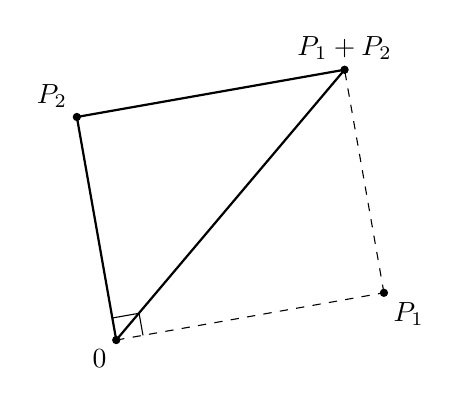
\begin{tikzpicture}[>=latex]
  \coordinate (O)  at (0,0);
  \coordinate (P1) at (3.4,0.6);
  \coordinate (P2) at (-0.5,2.833);
  \coordinate (P)  at (2.9,3.433);
  
  \draw[thick] (O) -- (P2);
  \draw[thick] (P2) -- (P);
  \draw[thick] (O) -- (P);
  
  \draw[dashed] (O) -- (P1);
  \draw[dashed] (P1) -- (P);
  
  % 直角标记
  \draw (0.34,0.06) -- (0.29,0.34) -- (-0.05,0.28);
  
  \fill (O)  circle (1.5pt) node[below left]{$0$};
  \fill (P1) circle (1.5pt) node[below right]{$P_1$};
  \fill (P2) circle (1.5pt) node[above left]{$P_2$};
  \fill (P)  circle (1.5pt) node[above]{$P_1 + P_2$};
\end{tikzpicture}
\end{center}

本章的主题是研究有限维 $\mathbb{R}$-和 $\mathbb{C}$-向量空间 $V$, 它们配备有由数量积 $\langle \cdot, \cdot \rangle \colon V \times V \longrightarrow K$ 给出的距离函数, 其中对 $K$ 要分别代入所考虑的基础域 $\mathbb{R}$ 或 $\mathbb{C}$.此时我们称为欧几里得或\emph{酉向量空间}(\textup{unitärer Vektorraum})\index{youxiangliangkongjian@酉向量空间(unitärer Vektorraum)}.最重要的例子是带有数量积 $\langle x, y \rangle = \sum_{i = 1}^{n} x_i \overline{y}_i$ 的向量空间 $K^n$, 其中 $\overline{y}_i$ 分别表示与 $y_i$ 共轭的复数.每个数量积都满足\emph{柯西-施瓦茨不等式}(\textup{Schwarz'sche Ungleichung})\index{kexishiwacibudengshi@柯西-施瓦茨不等式(Schwarz'sche Ungleichung)} $|\langle x, y \rangle| \leq |x| \, |y|$($x, y \in V$), 由它特别还可得到\emph{三角不等式}(\textup{Dreiecksungleichung})\index{sanjiaobudengshi@三角不等式(Dreiecksungleichung)} $|x + y| \leq |x| + |y|$.

作为基本工具, 我们将讨论以 E.~施密特(E. Schmidt)命名的\emph{正交规范化方法}(\textup{Schmidt'sches Orthonormalisierungsverfahren})\index{zhengjiaoguifanhuafangfa@正交规范化方法(Schmidt'sches Orthonormalisierungsverfahren)}.它允许我们从一个任意的基 $x_1, \ldots, x_n$ 出发, 通过逐次改变诸 $x_i$, 构造出一个所谓的\emph{标准正交基}(\textup{Orthonormalbasis})\index{biaozhunzhengjiaoji@标准正交基(Orthonormalbasis)} $e_1, \ldots, e_n$, 它满足 $|e_i| = 1$ 对一切 $i$ 以及 $\langle e_i, e_j \rangle = 0$ 对一切 $i \neq j$ 成立.这样的标准正交基于是可以看作 $V$ 中的一个直角坐标系.此外, 由于双线性性, $V$ 的数量积可以很容易地借助 $V$ 的一个标准正交基重新构造出来, 因此一个带有数量积形式的距离函数的向量空间 $V$, 只要知道了 $V$ 中的一个标准\emph{正交基}(\textup{Orthogonalbasis})\index{zhengjiaoji@正交基(Orthogonalbasis)}, 就已经被完全确定.

在第 6 章中, 我们研究了有限维向量空间 $V$(系数在任意域 $K$ 中)上自同态 $f \colon V \longrightarrow V$ 的标准形.例如, 若 $f$ 关于 $V$ 的某个基 $X$ 由矩阵 $A_{f, X, X}$ 给出, 那么问题就在于寻找一个基变换矩阵 $A_{\id, X', X}$, 使得矩阵

\[
A_{f, X', X'} = (A_{\id, X', X})^{-1} \cdot A_{f, X, X} \cdot A_{\id, X', X}
\]

具有尽可能"简单"的形式.换言之, 我们借助标准形理论确定了 $K^{n \times n}$ 中矩阵的相似类, 其中两个矩阵 $A, B \in K^{n \times n}$ 称为相似的, 如果存在可逆矩阵 $S \in \mathrm{Gl}(n, K)$ 使得 $B = S^{-1} \cdot A \cdot S$ 成立.

现在我们想也在欧几里得与酉向量空间 $V$ 的框架内处理一个类似的问题.不过这里我们必须把 $V$ 上的距离函数一并考虑在内.因此我们只允许这样的基变换矩阵 $A_{\id, X', X}$, 它们保持长度, 从而定义出标准正交基 $X$ 与 $X'$ 之间的变换.后者恰好发生在

\[
(A_{\id, X', X})^{-1} = (A_{\id, X', X})^* := \overline{A_{\id, X', X}}^{t}
\]

成立的情形, 其中对矩阵 $A = (\alpha_{ij}) \in K^{n \times n}$, 相应的复\emph{共轭矩阵}(\textup{konjugierte Matrix})\index{gongejuzhen@共轭矩阵(konjugierte Matrix)} $\overline{A}$ 由 $\overline{A} = (\overline{\alpha}_{ij})$ 给出; 具有上述性质的矩阵 $S = A_{\id, X', X}$ 称为\emph{正交}(\textup{orthogonal})\index{zhengjiao@正交(orthogonal)}的(当 $K = \mathbb{R}$)或酉的(当 $K = \mathbb{C}$).由这样的矩阵定义的 $K^{n \times n}$ 中矩阵的等价关系, 因而比第 6 章所考虑的一般矩阵等价关系要严密得多.所以对标准形问题, 把注意力限制在 $K^{n \times n}$ 的某些子类上是合理的.我们在这里本质上只考虑\emph{对称矩阵}(\textup{symmetrische Matrix})\index{duichenjuzhen@对称矩阵(symmetrische Matrix)}或\emph{埃尔米特矩阵}(\textup{hermitesche Matrix})\index{aiermitejuzhen@埃尔米特矩阵(hermitesche Matrix)}, 即满足 $A = A^*$ 的矩阵 $A \in K^{n \times n}$; 关于标准正交基, 它们恰好代表所谓的自\emph{伴随自同态}(\textup{adjungierter Endomorphismus})\index{bansuizitongtai@伴随自同态(adjungierter Endomorphismus)} $f \colon V \longrightarrow V$, 后者满足关系 $\langle f(x), y \rangle = \langle x, f(y) \rangle$($x, y \in V$).不过此时我们能够证明一个令人惊讶的事实: 这样的矩阵在借助正交或\emph{酉矩阵}(\textup{unitäre Matrix})\index{youjuzhen@酉矩阵(unitäre Matrix)}的,更严格的等价意义下, 总是等价于一个实对角矩阵.

在上述分类问题中获得的成果, 也可以富有成效地应用于有限维 $K$-向量空间 $V$ 上对称\emph{双线性形式}(\textup{Bilinearform})\index{shuangxianxingxingshi@双线性形式(Bilinearform)}(当 $K = \mathbb{R}$)或\emph{埃尔米特形式}(\textup{hermitesche Form; HF})\index{aiermitexingshi@埃尔米特形式(hermitesche Form; HF)}(当 $K = \mathbb{C}$)的分类, 即应用于相应的映射 $\varphi \colon V \times V \longrightarrow K$.因为它们也是关于 $V$ 的一个基 $X$ 由满足关系 $A_{\varphi, X} = A_{\varphi, X}^*$ 的矩阵 $A_{\varphi, X}$ 来描述的.不过, 在基变换下的变换行为与自同态的情形不同, 即为

\[
A_{\varphi, X'} = A_{\id, X', X}^{t} \cdot A_{\varphi, X} \cdot \overline{A_{\id, X', X}}\text{.}
\]

但如果我们在欧几里得或酉向量空间的框架内活动, 只允许正交或酉的基变换矩阵, 那么成立 $A_{\id, X', X}^{t} = \overline{A_{\id, X', X}}^{-1}$, 从而变换行为与 $V$ 的自同态类似.于是我们可以利用自伴随自同态的分类, 并且对欧几里得或酉向量空间得到: 对称双线性形式或埃尔米特形式的类由实对角矩阵表示(\emph{主轴变换}(\textup{Hauptachsentransformation})\index{zhuzhoubianhuan@主轴变换(Hauptachsentransformation)}定理).此时比较容易看出, 相应的类在一般等价(借助 $\mathrm{Gl}(n, K)$ 中可逆矩阵)的意义下由对角线元素可取 $1$, $-1$, $0$ 这三个值的对角矩阵表示(西尔维斯特惯性定律).

"主轴变换"这一称谓指出了具体的几何事实.当 $K = \mathbb{R}$ 时, 例如考虑 $\mathbb{R}^n$ 上由

\[
q(x) = \sum_{i \leq j;\, i, j = 1, \ldots, n} \alpha_{ij} x_i x_j
\]

(其中 $\alpha_{ij} \in \mathbb{R}$ 为某些常数)给出的\emph{二次型}(\textup{quadratische Form})\index{ercixing@二次型(quadratische Form)}, 以及由 $q(x) = c$($c \in \mathbb{R}$)给出的几何图形.于是可以把对称双线性形式

\[
\langle \cdot, \cdot \rangle \colon \mathbb{R}^n \times \mathbb{R}^n \longrightarrow \mathbb{R}, \qquad \langle x, y \rangle = \frac{1}{2}\bigl(q(x + y) - q(x) - q(y)\bigr)
\]

赋给 $q$; 对这个形式有 $q(x) = \langle x, x \rangle$.在这种情形下, 主轴变换定理断言: 存在 $\mathbb{R}^n$ 中一个新的直角坐标系 $e_1', \ldots, e_n'$, 使得 $q$ 关于新坐标以

\[
q'(x') = \sum_{i = 1}^{n} \lambda_i x_i'^2
\]

的形式被描述, 其中 $\lambda_i \in \mathbb{R}$ 为某些数.例如取 $n = 2$ 并假定 $\lambda_1, \lambda_2, c > 0$, 那么 $q(x) = c$ 就描述一个椭圆, 其轴最初不必与给定的坐标系 $e_1, e_2$ 的轴一致.主轴变换恰好断言: 通过正交的基变换可以做到, 使新坐标系 $e_1', e_2'$ 的轴与椭圆的轴一致:

\begin{center}
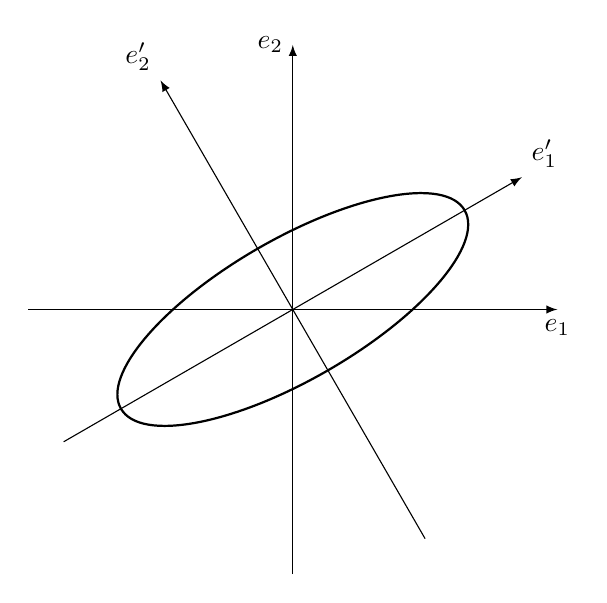
\begin{tikzpicture}[>=latex, scale=1.05]
  % 原坐标系 e_1, e_2
  \draw[->] (-3.2,0) -- (3.2,0) node[below]{$e_1$};
  \draw[->] (0,-3.2) -- (0,3.2) node[left]{$e_2$};
  
  \begin{scope}[rotate=30]
    % 椭圆
    \draw[thick] (0,0) ellipse (2.4 and 0.85);
    % 主轴新坐标系 e_1', e_2'
    \draw[->] (-3.2,0) -- (3.2,0) node[above right]{$e_1'$};
    \draw[->] (0,-3.2) -- (0,3.2) node[above left]{$e_2'$};
  \end{scope}
\end{tikzpicture}
\end{center}

\section{半双线性形式}\label{sec:7.1}

在下面的讨论中, 我们将只考虑系数域为 $\mathbb{R}$ 或 $\mathbb{C}$ 的向量空间, 并且通常用 $K$ 代替 $\mathbb{R}$ 或 $\mathbb{C}$ 来书写.特别是对 $\mathbb{C}$, 复\emph{共轭映射}(\textup{Konjugationsabbildung})\index{gongeyingshe@共轭映射(Konjugationsabbildung)}

\[
\mathbb{C} \longrightarrow \mathbb{C}, \qquad a \longmapsto \overline{a},
\]

将具有重要意义, 其中对 $a = \alpha + i \beta$($\alpha, \beta \in \mathbb{R}$), 相应的复共轭数由 $\overline{a} = \alpha - i \beta$ 给出.共轭映射 $a \longmapsto \overline{a}$ 表示 $\mathbb{C}$ 上的一个所谓的对合, 即一个满足 $\sigma^2 = \id$ 的自同构 $\sigma \colon \mathbb{C} \longrightarrow \mathbb{C}$, 并且还成立 $\sigma|_{\mathbb{R}} = \id$.对 $a = \alpha + i \beta \in \mathbb{C}$($\alpha, \beta \in \mathbb{R}$), 人们把

\[
\alpha = \frac{1}{2}(a + \overline{a}) = \operatorname{Re}(a)
\]

称为 $a$ 的实部, 把

\[
\beta = \frac{1}{2i}(a - \overline{a}) = \operatorname{Im}(a)
\]

称为 $a$ 的虚部, 并把

\[
|a| = \sqrt{\alpha^2 + \beta^2} = \sqrt{a \cdot \overline{a}}
\]

称为 $a$ 的绝对值.此时成立如下等价关系:

\[
a \in \mathbb{R} \Longleftrightarrow \operatorname{Re}(a) = a \Longleftrightarrow \operatorname{Im}(a) = 0 \Longleftrightarrow a = \overline{a}\text{.}
\]

对特殊元素 $a \in K$, 我们在后面也将考虑形如 $a \geq 0$ 或 $a > 0$ 的条件.这里的意思是 $a$ 为实数, 即满足 $a \in \mathbb{R} \subset K$, 并且此外满足条件 $a \geq 0$ 或 $a > 0$.

\begin{definition}[\emph{半双线性形式}\index{banshuangxianxingxingshi@半双线性形式(Sesquilinearform)}]\label{def:7.1.1}\index{banshuangxianxingxingshi@半双线性形式(Sesquilinearform)}
设 $V$ 是一个 $K$-向量空间.一个映射 $\varphi \colon V \times V \longrightarrow K$ 称为半双线性形式(sesqui = 一倍半), 如果对 $x, x_1, x_2, y, y_1, y_2 \in V$ 以及 $\alpha \in K$ 成立:
\begin{enumerate}
\item[(i)] $\varphi(x_1 + x_2, y) = \varphi(x_1, y) + \varphi(x_2, y)$;
\item[(ii)] $\varphi(\alpha x, y) = \alpha \varphi(x, y)$;
\item[(iii)] $\varphi(x, y_1 + y_2) = \varphi(x, y_1) + \varphi(x, y_2)$;
\item[(iv)] $\varphi(x, \alpha y) = \overline{\alpha} \varphi(x, y)$.
\end{enumerate}
\end{definition}

当 $K = \mathbb{R}$ 时恒有 $\alpha = \overline{\alpha}$, 此时人们也把它称为双线性形式 $\varphi$.如果满足

\[
\begin{array}{l}
\varphi(x, y) = 0 \ \text{对一切} \ y \in V \ \text{推出} \ x = 0, \\
\varphi(x, y) = 0 \ \text{对一切} \ x \in V \ \text{推出} \ y = 0,
\end{array}
\]

则称 $\varphi$ 为非退化的.

为得到一个简单的例子, 令 $V = K$.那么对固定的 $a \in K$, 由

\[
\varphi(x, y) = a \cdot x \cdot \overline{y}
\]

定义了 $V$ 上的一个半双线性形式, 并且它恰在 $a \neq 0$ 时非退化.

\begin{definition}[对称双线性形式与埃尔米特形式]\label{def:7.1.2}\index{shuangxianxingxingshi@双线性形式(Bilinearform)}\index{duichenshuangxianxingxingshi@对称双线性形式(symmetrische Bilinearform)}\index{aiermitexingshi@埃尔米特形式(hermitesche Form; HF)}
满足

\[
\varphi(x, y) = \overline{\varphi(y, x)} \quad \text{对一切} \quad x, y \in V
\]

的半双线性形式 $\varphi \colon V \times V \longrightarrow K$, 当 $K = \mathbb{R}$ 时称为对称双线性形式(简称 sBF), 当 $K = \mathbb{C}$ 时称为埃尔米特形式(简称 HF).对这样的形式, 人们经常用记号 $\langle x, y \rangle$ 代替 $\varphi(x, y)$.特别地, 此时对一切 $x \in V$ 成立 $\varphi(x, x) = \langle x, x \rangle \in \mathbb{R}$.
\end{definition}

例如,

\[
\varphi \colon K^n \times K^n \longrightarrow K, \qquad (x, y) \longmapsto x^t \cdot \overline{y},
\]

定义一个 sBF 或 HF, 其中这个映射详细写出来为:

\[
\bigl((x_1, \ldots, x_n)^t, (y_1, \ldots, y_n)^t\bigr) \longmapsto \sum_{i = 1}^{n} x_i \cdot \overline{y}_i\text{.}
\]

容易看出形式 $\varphi$ 是非退化的, 因为例如对 $x \neq 0$ 成立 $\varphi(x, x) > 0$.另一方面, 通过规定

\[
\bigl((x_1, \ldots, x_n)^t, (y_1, \ldots, y_n)^t\bigr) \longmapsto \sum_{i = 1}^{r} x_i \cdot \overline{y}_i,
\]

其中只求和到某个 $r < n$, 则在 $K^n$ 上定义了一个退化的形式.

\begin{definition}[\emph{正定}\index{zhengding@正定(positiv definit)}与数量积]\label{def:7.1.3}\index{zhengding@正定(positiv definit)}\index{shuliangji@数量积(Skalarprodukt)}
一个 sBF 或 HF $\varphi \colon V \times V \longrightarrow K$ 称为\emph{正半定}(\textup{positiv semi-definit})\index{zhengbanding@正半定(positiv semi-definit)}的, 如果对一切 $x \in V$ 成立 $\varphi(x, x) \geq 0$.如果甚至对一切 $x \in V - \{0\}$ 成立 $\varphi(x, x) > 0$, 则称 $\varphi$ 为正定的.此时人们也称 $\varphi$ 为 $V$ 上的一个数量积, 并把二元组 $(V, \varphi)$, 当 $K = \mathbb{R}$ 时称为\emph{欧几里得向量空间}(\textup{euklidischer Vektorraum})\index{oujilidexiangliangkongjian@欧几里得向量空间(euklidischer Vektorraum)}, 当 $K = \mathbb{C}$ 时称为酉向量空间.
\end{definition}

上面考察过的形式 $K^n \times K^n \longrightarrow K$, $(x, y) \longmapsto x^t \cdot \overline{y}$ 例如定义了 $K^n$ 上的一个数量积, 即所谓标准数量积.

\begin{theorem}[柯西-施瓦茨不等式]\label{thm:7.1.4}\index{kexishiwacibudengshi@柯西-施瓦茨不等式(Schwarz'sche Ungleichung)}
设 $\varphi \colon V \times V \longrightarrow K$, $(x, y) \longmapsto \langle x, y \rangle$ 是 $K$-向量空间 $V$ 上的正半定 sBF 或 HF.则对 $x, y \in V$ 成立下列不等式:

\[
|\langle x, y \rangle|^2 \leq \langle x, x \rangle \cdot \langle y, y \rangle\text{.}
\]

若 $\varphi$ 甚至正定, 则在这个公式中恰在 $x$ 与 $y$ 线性相关时成立等号.
\end{theorem}

\begin{proof}
任取 $\alpha, \beta \in K$.则成立

\[
\begin{array}{l}
0 \leq \langle \alpha x + \beta y, \alpha x + \beta y \rangle \\
= \alpha \overline{\alpha} \langle x, x \rangle + \alpha \overline{\beta} \langle x, y \rangle + \beta \overline{\alpha} \langle y, x \rangle + \beta \overline{\beta} \langle y, y \rangle \\
= \alpha \overline{\alpha} \langle x, x \rangle + 2\operatorname{Re}\bigl(\alpha \overline{\beta} \langle x, y \rangle\bigr) + \beta \overline{\beta} \langle y, y \rangle\text{.}
\end{array}
\]

若现在 $\langle x, x \rangle = \langle y, y \rangle = 0$, 则特别取 $\alpha = -1$ 与 $\beta = \langle x, y \rangle$.由此得

\[
0 \leq 2\operatorname{Re}\bigl(\alpha \overline{\beta} \langle x, y \rangle\bigr) = -2|\langle x, y \rangle|^2 \leq 0
\]

从而 $\langle x, y \rangle = 0$, 于是特别地

\[
|\langle x, y \rangle|^2 \leq \langle x, x \rangle \cdot \langle y, y \rangle\text{.}
\]

现在设 $\langle x, x \rangle > 0$.在此情形下取

\[
\alpha = -\overline{\langle x, y \rangle}, \qquad \beta = \langle x, x \rangle\text{.}
\]

于是得

\[
\begin{array}{c}
0 \leq |\langle x, y \rangle|^2 \langle x, x \rangle - 2|\langle x, y \rangle|^2 \langle x, x \rangle + \langle x, x \rangle^2 \langle y, y \rangle \\
= -|\langle x, y \rangle|^2 \langle x, x \rangle + \langle x, x \rangle^2 \langle y, y \rangle,
\end{array}
\]

即正如所期望的

\[
|\langle x, y \rangle|^2 \leq \langle x, x \rangle \cdot \langle y, y \rangle\text{.}
\]

情形 $\langle y, y \rangle > 0$ 可类似地处理.

若最后 $x, y \in V$ 线性相关, 则其中一个向量是另一个的倍数, 并且毫无困难地得到

\[
|\langle x, y \rangle|^2 = \langle x, x \rangle \cdot \langle y, y \rangle\text{.}
\]

反之, 若这个等式成立, 则如上取 $\alpha = -\overline{\langle x, y \rangle}$, $\beta = \langle x, x \rangle$ 得到

\[
\begin{array}{c}
\langle \alpha x + \beta y, \alpha x + \beta y \rangle \\
= |\langle x, y \rangle|^2 \langle x, x \rangle - 2|\langle x, y \rangle|^2 \langle x, x \rangle + \langle x, x \rangle^2 \langle y, y \rangle = 0\text{.}
\end{array}
\]

若 $\varphi$ 正定, 则由此得 $\alpha x + \beta y = 0$, 并且可以看到 $x, y$ 线性相关.因为对 $x = 0$ 这是显然的, 对 $x \neq 0$ 也如此, 因为此时系数 $\beta = \langle x, x \rangle$ 由 $\varphi$ 的正定性而不消失.
\end{proof}

\begin{corollary}\label{cor:7.1.5}
设 $\varphi \colon V \times V \longrightarrow K$ 是正半定 sBF 或 HF.则 $\varphi$ 正定, 当且仅当 $\varphi$ 非退化.
\end{corollary}

若 $\varphi \colon V \times V \longrightarrow K$ 是正半定 sBF 或 HF, 则对一切 $x \in V$ 成立 $\langle x, x \rangle \geq 0$, 并且人们把 $|x| = \sqrt{\langle x, x \rangle}$ 称为向量 $x \in V$(关于 $\varphi$)的长度或模长.如此定义的向量模长满足通常的三角不等式:

\begin{corollary}[三角不等式]\label{cor:7.1.6}\index{sanjiaobudengshi@三角不等式(Dreiecksungleichung)}
设 $\varphi \colon V \times V \longrightarrow K$ 是正半定 sBF 或 HF.则对 $x, y \in V$ 成立

\[
|x + y| \leq |x| + |y|\text{.}
\]
\end{corollary}

\begin{proof}
成立

\[
\begin{array}{r l}
|x + y|^2 & = \langle x + y, x + y \rangle \\
& = \langle x, x \rangle + 2\operatorname{Re}\bigl(\langle x, y \rangle\bigr) + \langle y, y \rangle \\
& \leq \langle x, x \rangle + 2|\langle x, y \rangle| + \langle y, y \rangle \\
& \leq |x|^2 + 2|x| \, |y| + |y|^2 \\
& = \bigl(|x| + |y|\bigr)^2
\end{array}
\]

从而 $|x + y| \leq |x| + |y|$.
\end{proof}

关于向量模长的进一步性质, 我们还可以列举: 对 $\alpha \in K$, $x \in V$ 成立 $|\alpha x| = |\alpha| \, |x|$.若 $\varphi$ 甚至正定, 则 $|x| = 0$ 等价于 $x = 0$.此外, 若 $\langle x, x \rangle = 1$ 从而 $|x| = 1$ 成立, 则称向量 $x \in V$ 为规范化的(normiert).例如对 $|x| \neq 0$ 的 $x \in V$, $\frac{x}{|x|}$ 是规范化的.

最后我们想借助几何直观解释 $\mathbb{R}^n$ 上的标准数量积.首先, 我们利用勾股定理确认, 向量 $x \in \mathbb{R}^n$ 的模长恰与点 $x$ 到原点的通常欧几里得距离一致.若 $e \in \mathbb{R}^n$ 是另一个向量且成立 $|e| = 1$, 则如下方程成立:

\[
|x|^2 = \langle x, e \rangle^2 + |x - \langle x, e \rangle e|^2\text{.}
\]

这容易直接验算.依据勾股定理的逆定理, 这在几何上意味着边长为 $|x|$, $|\langle x, e \rangle|$ 与 $|x - \langle x, e \rangle e|$ 的三角形是直角三角形:

\begin{center}
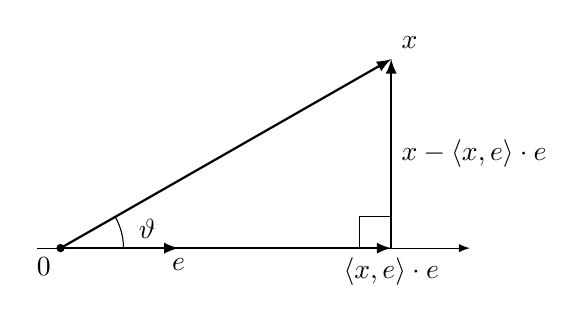
\begin{tikzpicture}[>=latex]
  \coordinate (O) at (0,0);
  \coordinate (E) at (1.5,0);
  \coordinate (P) at (4.2,0);
  \coordinate (X) at (4.2,2.4);
  
  \draw[->] (-0.3,0) -- (5.2,0);
  \draw[thick, ->] (O) -- (E) node[below]{$e$};
  \draw[thick, ->] (O) -- (P);
  \node[below] at (P) {$\langle x, e \rangle \cdot e$};
  
  \draw[thick, ->] (O) -- (X) node[above right]{$x$};
  \draw[thick, ->] (P) -- (X) node[midway, right]{$x - \langle x, e \rangle \cdot e$};
  
  % 直角标记
  \draw (3.8,0) -- (3.8,0.4) -- (4.2,0.4);
  
  % 夹角 vartheta
  \draw (0.8,0) arc (0:29.7:0.8);
  \node at (1.1,0.25) {$\vartheta$};
  
  \fill (O) circle (1.5pt) node[below left]{$0$};
\end{tikzpicture}
\end{center}

于是, 向量 $\langle x, e \rangle \cdot e$ 是这样产生的: 把 $x$ \emph{垂直投影}(\textup{senkrechte Projektion})\index{chuizhitouying@垂直投影(senkrechte Projektion)}到由 $e$ 给出的线性子空间 $\mathbb{R} \cdot e \subset \mathbb{R}^n$ 上.一般地, 可以按这种方式计算两个向量 $x, y \in \mathbb{R}^n - \{0\}$ 的数量积.即在上面的讨论中令 $e = |y|^{-1} \cdot y$.于是, 除符号外, $\langle x, y \rangle$ 作为 $|y|$ 与 $x$ 在直线 $\mathbb{R} \cdot y \subset \mathbb{R}^n$ 上的垂直投影的模长之积而得到.更准确地说, $x$ 在 $\mathbb{R} \cdot y$ 上的投影可以用分析学中的余弦函数来描述.若 $\vartheta$ 是 $x$ 与 $y$ 所夹的角, 则这个投影计算为 $\frac{|x|}{|y|} \cdot \cos(\vartheta) \cdot y$, 于是得:

\begin{theorem}\label{thm:7.1.7}
对向量 $x, y \in \mathbb{R}^n - \{0\}$ 与标准数量积成立

\[
\langle x, y \rangle = |x| \cdot |y| \cdot \cos \vartheta,
\]

其中 $\vartheta$ 是 $x$ 与 $y$ 所夹的角.
\end{theorem}

用 $x - \langle x, e \rangle e$ 从 $x$ 构造一个垂直于 $e$ 的向量, 这种可能性恰好就是我们在下面的 \ref{sec:7.2} 节中将要讨论的 E.~施密特正交规范化方法的中心思想.

\aufgaben

如无特别说明, 设 $V$ 是有限维 $\mathbb{R}$-向量空间, $\varphi \colon V \times V \longrightarrow \mathbb{R}$ 是 $V$ 上的对称双线性形式.

\medskip
\noindent\textbf{习题 1.} 通过

\[
\ker \varphi = \bigl\{x \in V;\, \varphi(x, y) = 0 \ \text{对一切} \ y \in V\bigr\}
\]

定义 $\varphi$ 的核, 并证明 $\varphi$ 在 $V/\ker \varphi$ 上诱导出一个非退化的对称双线性形式.

\medskip
\noindent\textbf{习题 2.} 通过令 $q(x) = \varphi(x, x)$($x \in V$)定义与 $\varphi$ 相应的二次型 $q \colon V \longrightarrow \mathbb{R}$, 并证明 $\varphi$ 由 $q$ 唯一确定.

\medskip
\noindent\textbf{习题 3.} 设 $\varphi$ 正定.对 $x, y \in V$, $y \neq 0$, 考虑 $t \in \mathbb{R}$ 的多项式函数 $p(t) = |x + ty|^2$.求出 $p(t)$ 的全部零点, 并由此推出当 $K = \mathbb{R}$ 时定理~\mtref{thm:7.1.4} 版本下的柯西-施瓦茨不等式.(AT 360)

\medskip
\noindent\textbf{习题 4.} 设 $\varphi$ 正定.对 $x, y \in V - \{0\}$ 证明:
\begin{enumerate}
\item[(i)] 成立 $-1 \leq \dfrac{\varphi(x, y)}{|x| \cdot |y|} \leq 1$.由分析学知存在一个角度 $0 \leq \vartheta \leq \pi$ 使得 $\dfrac{\varphi(x, y)}{|x| \cdot |y|} = \cos \vartheta$.
\item[(ii)] 成立余弦定理:
\end{enumerate}

\[
|x - y|^2 = |x|^2 + |y|^2 - 2|x| \, |y| \cos \vartheta\text{.}
\]

\medskip
\noindent\textbf{习题 5.} 设 $V$ 是系数域 $K$ 上的向量空间, $V^*$ 是其对偶空间, $W$ 是所有 $K$-双线性映射 $V \times V \longrightarrow K$ 构成的 $K$-向量空间.证明: 把同态 $\varphi \colon V \longrightarrow V^*$ 映为映射

\[
V \times V \longrightarrow K, \qquad (x, y) \longmapsto \varphi(x)(y)
\]

的映射 $\operatorname{Hom}_K(V, V^*) \longrightarrow W$ 是 $K$-向量空间的同构.(AT 361)

\section{正交性}\label{sec:7.2}

\begin{definition}[正交]\label{def:7.2.1}\index{zhengjiao@正交(orthogonal)}
设 $\varphi \colon V \times V \longrightarrow K$, $(x, y) \longmapsto \langle x, y \rangle$ 是一个 sBF 或 HF.若 $\langle x, y \rangle = 0$ 成立, 则称两个向量 $x, y \in V$ 互相正交或互相垂直.$V$ 中满足 $0 \notin M$ 的一个向量组 $M$ 称为\emph{正交系}(\textup{Orthogonalsystem})\index{zhengjiaoxi@正交系(Orthogonalsystem)}, 如果 $M$ 中任意两个向量都互相正交.若此外对一切 $x \in M$ 成立 $\langle x, x \rangle = 1$, 则也称其为\emph{标准正交系}(\textup{Orthonormalsystem})\index{biaozhunzhengjiaoxi@标准正交系(Orthonormalsystem)}.
\end{definition}

\begin{remark}\label{rem:7.2.2}
设 $\varphi \colon V \times V \longrightarrow K$ 是一个数量积.若 $M$ 是 $V$ 中向量的正交系, 则 $M$ 线性无关.
\end{remark}

\begin{proof}
对 $M$ 的一个有限子系统 $x_1, \ldots, x_n$ 考虑满足 $\sum_{i = 1}^{n} \alpha_i x_i = 0$ 的系数 $\alpha_1, \ldots, \alpha_n \in K$.于是对 $j = 1, \ldots, n$ 得

\[
0 = \Bigl\langle \sum_{i = 1}^{n} \alpha_i x_i, x_j \Bigr\rangle = \sum_{i = 1}^{n} \alpha_i \langle x_i, x_j \rangle = \alpha_j \langle x_j, x_j \rangle
\]

从而因 $\langle x_j, x_j \rangle > 0$ 得 $\alpha_j = 0$.
\end{proof}

\begin{definition}[正交基与标准正交基]\label{def:7.2.3}\index{zhengjiaoji@正交基(Orthogonalbasis)}\index{biaozhunzhengjiaoji@标准正交基(Orthonormalbasis)}
设 $\varphi \colon V \times V \longrightarrow K$ 是一个数量积.如果 $V$ 中向量 $e_1, \ldots, e_n$ 组成的组 $M$ 满足下列条件, 则称 $M$ 为 $V$ 的正交基(或标准正交基):
\begin{enumerate}
\item[(i)] $M$ 是 $V$ 的一个基;
\item[(ii)] $M$ 是一个正交系(或标准正交系).
\end{enumerate}
\end{definition}

把向量表示为某个标准正交基 $M = (e_1, \ldots, e_n)$ 中元素的线性组合后, 它们之间的数量积可以按简单的方式计算:

\[
\begin{array}{c}
\Bigl\langle \sum_{i = 1}^{n} \alpha_i e_i, \sum_{i = 1}^{n} \beta_i e_i \Bigr\rangle = \sum_{i, j = 1}^{n} \alpha_i \overline{\beta}_j \langle e_i, e_j \rangle \\
= \sum_{i, j = 1}^{n} \alpha_i \overline{\beta}_j \delta_{ij} = \sum_{i = 1}^{n} \alpha_i \overline{\beta}_i
\end{array}
\]

例如考虑 $K^n$ 上的标准数量积, 则 $K^n$ 的标准基构成一个标准正交基.

下面我们讨论所谓的 E.~施密特正交规范化方法, 借助它可以, 把欧几里得或酉向量空间中的基改造成标准正交基.首先我们处理这个方法的核心步骤, 即我们在 \ref{sec:7.1} 节末尾已经针对 $K^n$ 上的标准数量积做过几何说明的那个步骤.

\begin{lemma}[\emph{正交投影}\index{zhengjiaotouying@正交投影(orthogonale Projektion)}]\label{lem:7.2.4}\index{zhengjiaotouying@正交投影(orthogonale Projektion)}
设 $\varphi \colon V \times V \longrightarrow K$ 是一个数量积, $e_1, \ldots, e_k$ 是子空间 $U \subset V$ 的一个标准正交基.则

\[
p_U \colon V \longrightarrow U, \qquad x \longmapsto \sum_{j = 1}^{k} \langle x, e_j \rangle e_j,
\]

是一个满的 $K$-线性映射, 即所谓的到 $U$ 上的正交投影.它限制在 $U$ 上为恒等映射, 并且此外还满足方程 $\langle x - p_U(x), y \rangle = 0$($x \in V$, $y \in U$).由这个方程, $p_U$ 作为 $K$-线性映射 $V \longrightarrow U$ 被唯一确定.
\end{lemma}

\begin{proof}
由于形式 $\langle x, y \rangle$ 对 $x$ 是 $K$-线性的, 映射 $p_U$ 是 $K$-线性的.若又设 $x = \sum_{i = 1}^{k} \alpha_i e_i \in U$, 则

\[
\langle x, e_j \rangle = \Bigl\langle \sum_{i = 1}^{k} \alpha_i e_i, e_j \Bigr\rangle = \sum_{i = 1}^{k} \alpha_i \langle e_i, e_j \rangle = \alpha_j,
\]

并且特别地得 $p_U|_U = \id_U$.此外得

\[
\begin{array}{c}
\langle x - p_U(x), e_j \rangle = \langle x, e_j \rangle - \Bigl\langle \sum_{i = 1}^{k} \langle x, e_i \rangle e_i, e_j \Bigr\rangle \\
= \langle x, e_j \rangle - \langle x, e_j \rangle \langle e_j, e_j \rangle = 0,
\end{array}
\]

即 $x - p_U(x)$ 与 $e_1, \ldots, e_k$ 正交, 从而与 $U$ 正交.

若 $q_U \colon V \longrightarrow U$ 是任意一个满足 $\langle x - q_U(x), y \rangle = 0$($x \in V$, $y \in U$)的线性映射, 则特别地对 $x \in V$, $y \in U$ 成立 $\langle p_U(x) - q_U(x), y \rangle = 0$.由于 $V$ 的数量积限制为 $U$ 上的一个数量积, 必对 $x \in V$ 有 $p_U(x) - q_U(x) = 0$, 从而 $p_U = q_U$.
\end{proof}

若 $x_1, \ldots, x_n$ 是欧几里得或酉 $K$-向量空间的一个基, 那么可以先规范化 $x_1$, 即考虑向量 $e_1 = |x_1|^{-1} \cdot x_1$.然后可以依据引理~\mtref{lem:7.2.4} 作 $V$ 到子空间 $U_1 = K e_1$ 上的投影 $p_1$.向量 $e_2' = x_2 - p_1(x_2)$ 此时与 $e_1$ 正交, 并且 $e_1$ 连同 $|e_2'|^{-1} \cdot e_2'$ 组成一个标准正交系 $e_1, e_2$.按这种方式继续下去, 就可以把基 $x_1, \ldots, x_n$ 正交规范化, 即整体地转化为一个标准正交基.我们想把这一结果在这里更精确地表述并证明.

\begin{theorem}[施密特正交规范化]\label{thm:7.2.5}\index{zhengjiaoguifanhuafangfa@正交规范化方法(Schmidt'sches Orthonormalisierungsverfahren)}
设 $\varphi \colon V \times V \longrightarrow K$ 是一个数量积, $x_1, \ldots, x_n$ 是 $V$ 的一个基.则存在唯一确定的向量 $e_1, \ldots, e_n \in V$, 使得
\begin{enumerate}
\item[(i)] $e_1, \ldots, e_n$ 是 $V$ 的一个标准正交基;
\item[(ii)] 对 $k = 1, \ldots, n$ 成立 $\bigoplus_{i = 1}^{k} K e_i = \bigoplus_{i = 1}^{k} K x_i$;
\item[(iii)] 对 $E_k = (e_1, \ldots, e_k)$ 与 $X_k = (x_1, \ldots, x_k)$, 基变换矩阵 $A_k = A_{\id, E_k, X_k}$ 满足 $\det(A_k) > 0$, $k = 1, \ldots, n$.
\end{enumerate}

更准确地说, 诸向量 $e_k$($k = 1, \ldots, n$)可以按如下的归纳方式构造:

\[
e_k = \Bigl|x_k - \sum_{j = 1}^{k-1} \langle x_k, e_j \rangle e_j\Bigr|^{-1} \cdot \Bigl(x_k - \sum_{j = 1}^{k-1} \langle x_k, e_j \rangle e_j\Bigr)\text{.}
\]
\end{theorem}

\begin{proof}
我们首先证明存在性断言, 并对此对 $n$ 作归纳.归纳起点 $n = 0$ 是平凡的.设 $n > 0$, 并设 $e_1, \ldots, e_{n-1}$ 是具有所期望性质的 $U_{n-1} = \bigoplus_{i = 1}^{n-1} K x_i$ 的一个标准正交基.此时有 $x_n \notin U_{n-1} = \bigoplus_{i = 1}^{n-1} K e_i$, 故 $x_n - p_{n-1}(x_n)$ 不为零; 这里 $p_{n-1} \colon V \longrightarrow U_{n-1}$ 是依据引理~\mtref{lem:7.2.4} 的投影.于是

\[
e_n = \bigl|x_n - p_{n-1}(x_n)\bigr|^{-1} \cdot \bigl(x_n - p_{n-1}(x_n)\bigr)
\]

是良定义的, 并且由注记~\mtref{rem:7.2.2} 与引理~\mtref{lem:7.2.4} 可知 $e_1, \ldots, e_n$ 构成 $V$ 的一个标准正交基.此外, 由 $e_n$ 的定义存在形如

\[
e_n = \alpha \cdot x_n + y
\]

的方程, 其中常数 $\alpha > 0$, 向量 $y \in U_{n-1}$.由此得

\[
A_n = \begin{pmatrix} A_{n-1} & * \\ 0 & \alpha \end{pmatrix},
\]

并且由 $\alpha > 0$, $\det(A_{n-1}) > 0$ 得 $\det(A_n) = \alpha \cdot \det(A_{n-1}) > 0$.

为证明唯一性断言, 设 $f_1, \ldots, f_n$ 是 $V$ 的一个满足性质 (ii) 和 (iii) 的标准正交基.我们再次对 $n$ 作归纳来证明 $f_i = e_i$($i = 1, \ldots, n$), 其中归纳起点 $n = 0$ 是平凡的.设 $n > 0$.由归纳假设可以假定 $f_i = e_i$($i = 1, \ldots, n-1$).于是存在形如 $f_n = \alpha \cdot x_n + y$ 的方程, 其中 $\alpha \in K$, $y \in U_{n-1} = \bigoplus_{i = 1}^{n-1} K x_i$.基变换矩阵 $A_{\id, E', X}$, 其中我们使用基 $E' = (f_1, \ldots, f_n) = (e_1, \ldots, e_{n-1}, f_n)$ 与 $X = (x_1, \ldots, x_n)$, 此时具有形式

\[
A = \begin{pmatrix} A_{n-1} & * \\ 0 & \alpha \end{pmatrix},
\]

并且由 $\det(A)$, $\det(A_{n-1}) > 0$ 得 $\alpha > 0$.利用 $U_{n-1} = \bigoplus_{i = 1}^{n-1} K e_i$, 可以把 $y$ 写成 $e_1, \ldots, e_{n-1}$ 的线性组合.于是存在常数 $\beta_1, \ldots, \beta_{n-1} \in K$ 使得

\[
f_n = \alpha \cdot \Bigl(x_n - \sum_{i = 1}^{n-1} \beta_i e_i\Bigr)\text{.}
\]

对 $i = 1, \ldots, n-1$ 此时成立

\[
0 = \langle f_n, e_i \rangle = \alpha \cdot \bigl(\langle x_n, e_i \rangle - \beta_i\bigr),
\]

即 $\beta_i = \langle x_n, e_i \rangle$, 即

\[
f_n = \alpha \cdot \Bigl(x_n - \sum_{i = 1}^{n-1} \langle x_n, e_i \rangle e_i\Bigr)\text{.}
\]

由方程

\[
1 = |f_n| = \alpha \cdot \Bigl|x_n - \sum_{i = 1}^{n-1} \langle x_n, e_i \rangle e_i\Bigr|
\]

于是得

\[
\alpha = \Bigl|x_n - \sum_{i = 1}^{n-1} \langle x_n, e_i \rangle e_i\Bigr|^{-1}
\]

从而 $f_n = e_n$, 这正是所要证明的.
\end{proof}

\begin{corollary}\label{cor:7.2.6}
每个有限维欧几里得或酉向量空间 $V$ 都有一个标准正交基.子空间 $U \subset V$ 的每个标准正交基都可以扩充为 $V$ 的一个标准正交基.
\end{corollary}

\begin{corollary}\label{cor:7.2.7}
设 $V$ 是有限维欧几里得或酉向量空间, $V_1 \subset V_2 \subset \cdots \subset V_r = V$ 是 $K$-子空间的一个链.设 $\dim_K V_i = n_i$.则存在 $V$ 的一个标准正交基 $e_1, \ldots, e_n$, 使得 $e_1, \ldots, e_{n_i}$ 分别是 $V_i$ 的标准正交基, $i = 1, \ldots, r$.
\end{corollary}

若 $V$ 是带 sBF 或 HF 的 $K$-向量空间, 则当恒有 $\langle x, y \rangle = 0$($x \in M$, $y \in N$)时, 称两个子集 $M, N \subset V$ 正交, 记为 $M \perp N$.此时人们也写 $x \perp y$ 来代替 $\langle x, y \rangle = 0$, 其中 $x \perp y$ 等价于 $y \perp x$.此外, 对子集 $M \subset V$ 可以考察 $K$-子空间

\[
M^{\perp} = \bigl\{x \in V;\, x \perp y \ \text{对一切} \ y \in M\bigr\}\text{.}
\]

对子空间 $W \subset V$, 人们把 $W^{\perp}$ 称为 $W$ 在 $V$ 中的\emph{正交补}(\textup{orthogonales Komplement})\index{zhengjiaobu@正交补(orthogonales Komplement)}.

\begin{corollary}[正交补]\label{cor:7.2.8}\index{zhengjiaobu@正交补(orthogonales Komplement)}
设 $V$ 是有限维欧几里得或酉向量空间, $W \subset V$ 是一个子空间.则成立:
\begin{enumerate}
\item[(i)] $V = W \oplus W^{\perp}$, 特别地 $\dim_K W^{\perp} = \dim_K V - \dim_K W$;
\item[(ii)] $(W^{\perp})^{\perp} = W$.
\end{enumerate}
\end{corollary}

\begin{proof}
选取 $W$ 的一个标准正交基 $e_1, \ldots, e_r$, 并用元素 $e_{r+1}, \ldots, e_n$ 把它扩充为 $V$ 的一个标准正交基; 参见推论~\mtref{cor:7.2.6}.对 $W' = \bigoplus_{i = r+1}^{n} K e_i$ 此时成立 $W \perp W'$, 因而 $W' \subset W^{\perp}$.现在设 $x = \sum_{i = 1}^{n} \alpha_i e_i \in W^{\perp}$.方程 $\langle x, e_i \rangle = 0$($i = 1, \ldots, r$)此时表明 $\alpha_i = 0$($i = 1, \ldots, r$), 从而 $x \in W'$.因此成立 $W^{\perp} = W'$, 从而 $V = W \oplus W^{\perp}$.把这个论证应用于 $W^{\perp}$ 以代替 $W$, 便得到 $(W^{\perp})^{\perp} = W$.
\end{proof}

作为应用, 我们还想讨论 $\mathbb{R}^n$ 中平行多面体的体积.对线性无关的向量组 $x_1, \ldots, x_r \in \mathbb{R}^n$, 用

\[
P(x_1, \ldots, x_r) = \Bigl\{x \in \mathbb{R}^n;\, x = \sum_{i = 1}^{r} \alpha_i x_i \ \text{且} \ 0 \leq \alpha_i \leq 1\Bigr\}
\]

表示由这些向量张成的 $r$ 维平行多面体.若对 $r = n$, $x_1, \ldots, x_n$ 例如是 $\mathbb{R}^n$ 中的单位向量, 则 $P(x_1, \ldots, x_n)$ 恰为 $n$ 维单位立方体.

如通常一样, 我们把 $\mathbb{R}^n$ 看作带标准数量积的欧几里得向量空间.对一个 $r$ 维平行多面体 $P(x_1, \ldots, x_r)$, 考察由 $x_1, \ldots, x_r$ 生成的 $r$ 维子空间 $U \subset \mathbb{R}^n$, 并在 $U$ 中选取一个标准正交基 $M = (e_1, \ldots, e_r)$.然后设 $\det_M$ 是 $U$ 上在基 $M$ 上取值为 $1$ 的那个行列式函数; 参见定理~\mtref{thm:4.2.8}.在这种情形下, 平行多面体的体积定义为

\[
\operatorname{Vol}\bigl(P(x_1, \ldots, x_r)\bigr) = \bigl|\det_M(x_1, \ldots, x_r)\bigr|\text{.}
\]

自然要证明这个定义与 $U$ 的标准正交基 $M$ 的选取无关.我们还想说明, 这个体积与 $\mathbb{R}^n$ 中一个物体体积的直观观念一致.

\begin{theorem}[\emph{格拉姆行列式}\index{gelamuhanglieshi@格拉姆行列式(Gram'sche Determinante)}]\label{thm:7.2.9}\index{gelamuhanglieshi@格拉姆行列式(Gram'sche Determinante)}
对向量 $x_1, \ldots, x_r \in K^n$, 相应的格拉姆行列式定义为

\[
G(x_1, \ldots, x_r) = \det \begin{pmatrix}
\langle x_1, x_1 \rangle & \cdots & \langle x_1, x_r \rangle \\
\vdots & & \vdots \\
\langle x_r, x_1 \rangle & \cdots & \langle x_r, x_r \rangle
\end{pmatrix}
\]

其中 $\langle \cdot, \cdot \rangle$ 是 $K^n$ 上的标准数量积.成立 $G(x_1, \ldots, x_r) \geq 0$, 且 $G(x_1, \ldots, x_r)$ 恰在 $x_1, \ldots, x_r$ 线性相关时消失.

若 $x_1, \ldots, x_r$ 线性无关, $M = (e_1, \ldots, e_r)$ 是 $x_1, \ldots, x_r$ 在 $K^n$ 中生成的线性子空间的一个标准正交基, 则成立关系式

\[
G(x_1, \ldots, x_r) = \bigl|\det_M(x_1, \ldots, x_r)\bigr|^2\text{.}
\]
\end{theorem}

注意, 这个断言在 $r = 2$ 时恰好给出柯西-施瓦茨不等式(定理~\mtref{thm:7.1.4}), 而且独立于定理~\mtref{thm:7.1.4} 中给出的证明.此外我们还可以断言:

\begin{corollary}[平行多面体的体积]\label{cor:7.2.10}
平行多面体 $P(x_1, \ldots, x_r) \subset \mathbb{R}^n$ 的体积是良定义的, 且成立

\[
\operatorname{Vol}\bigl(P(x_1, \ldots, x_r)\bigr) = G(x_1, \ldots, x_r)^{\frac{1}{2}}\text{.}
\]
\end{corollary}

\begin{proof}[定理~\mtref{thm:7.2.9} 的证明]
若 $x_1, \ldots, x_r$ 线性相关, 则立即看出格拉姆行列式矩阵中的列或行线性相关, 故成立 $G(x_1, \ldots, x_r) = 0$.因此设 $x_1, \ldots, x_r$ 线性无关.于是这些向量生成一个 $r$ 维子空间 $U \subset K^n$, 它同样配备有数量积, 并且我们可以依据定理~\mtref{thm:7.2.5} 在 $U$ 中选取一个标准正交基 $M = (e_1, \ldots, e_r)$.若再用 $x_{1, M}, \ldots, x_{r, M}$ 表示 $x_1, \ldots, x_r$ 关于基 $M$ 的坐标列向量, 则成立

\[
(x_{1, M}, \ldots, x_{r, M})^t \cdot (\overline{x}_{1, M}, \ldots, \overline{x}_{r, M}) = \bigl(\langle x_i, x_j \rangle\bigr)_{i, j = 1, \ldots, r}\text{.}
\]

特别地得

\[
\bigl|\det_M(x_1, \ldots, x_r)\bigr|^2 = \bigl|\det(x_{1, M}, \ldots, x_{r, M})\bigr|^2 = G(x_1, \ldots, x_r)
\]

从而由 $x_1, \ldots, x_r$ 线性无关得 $G(x_1, \ldots, x_r) > 0$.
\end{proof}

现在我们还想说明, 平行多面体的上述体积

\[
\operatorname{Vol}\bigl(P(x_1, \ldots, x_r)\bigr) = \bigl|\det_M(x_1, \ldots, x_r)\bigr| = G(x_1, \ldots, x_r)^{\frac{1}{2}}
\]

(其中 $M = (e_1, \ldots, e_r)$ 是 $x_1, \ldots, x_r$ 在 $\mathbb{R}^n$ 中生成的子空间的一个标准正交基)在直观意义下也恰好对应 $P(x_1, \ldots, x_r)$ 的 $r$ 维体积.对 $r = 1$ 这是立即明白的.对 $r > 1$ 考察正交投影 $p_U \colon \mathbb{R}^n \longrightarrow U := \sum_{i = 1}^{r-1} \mathbb{R} x_i$.此时 $x_r' = x_r - p_U(x_r)$ 与 $U$ 正交, 从而与 $x_1, \ldots, x_{r-1}$ 正交.于是成立

\[
\begin{array}{c}
\operatorname{Vol}\bigl(P(x_1, \ldots, x_r)\bigr) = \bigl|\det_M(x_1, \ldots, x_r)\bigr| \\
= \bigl|\det_M(x_1, \ldots, x_{r-1}, x_r')\bigr| = \operatorname{Vol}\bigl(P(x_1, \ldots, x_{r-1}, x_r')\bigr)
\end{array}
\]

以及

\[
\begin{array}{l}
\operatorname{Vol}\bigl(P(x_1, \ldots, x_r)\bigr)^2 = \operatorname{Vol}\bigl(P(x_1, \ldots, x_{r-1}, x_r')\bigr)^2 \\
\qquad = \det \begin{pmatrix}
\langle x_1, x_1 \rangle & \cdots & \langle x_1, x_{r-1} \rangle & 0 \\
\vdots & \ddots & \vdots & \vdots \\
\langle x_{r-1}, x_1 \rangle & \cdots & \langle x_{r-1}, x_{r-1} \rangle & 0 \\
0 & \cdots & 0 & \langle x_r', x_r' \rangle
\end{pmatrix} \\
\qquad = \det \begin{pmatrix}
\langle x_1, x_1 \rangle & \cdots & \langle x_1, x_{r-1} \rangle \\
\vdots & \ddots & \vdots \\
\langle x_{r-1}, x_1 \rangle & \cdots & \langle x_{r-1}, x_{r-1} \rangle
\end{pmatrix} \cdot |x_r'|^2 \\
\qquad = \operatorname{Vol}\bigl(P(x_1, \ldots, x_{r-1})\bigr)^2 \cdot |x_r'|^2\text{.}
\end{array}
\]

现在 $|x_r'|$ 应解释为 $x_r$ 到 $U$ 的垂直距离; 关于这一点也参见本节末尾的习题 4.于是 $r$ 维平行多面体 $P(x_1, \ldots, x_r)$ 的体积, 作为 $(r-1)$ 维"底面"$P(x_1, \ldots, x_{r-1})$ 的体积与 $x_r$ 在此底面上方的"高"之积而得到.由归纳立刻可知, 平行多面体的上述体积与具有相同高度比的立方体的体积一致, 这与直观观念相符.

\aufgaben

\medskip
\noindent\textbf{习题 1.} 把 $\mathbb{R}^3$ 看作带标准数量积的欧几里得向量空间, 并把 E.~施密特正交规范化方法应用于基 $(1, 1, 0)$, $(1, 0, 1)$, $(0, 1, 1) \in \mathbb{R}^3$.

\medskip
\noindent\textbf{习题 2.} 对 $n \in \mathbb{N}$ 设 $\mathbb{R}[T]_n \subset \mathbb{R}[T]$ 是所有次数 $\leq n$ 的多项式构成的 $\mathbb{R}$-子空间.证明: 通过

\[
\langle f, g \rangle = \int_{0}^{1} f(t) g(t) \, dt, \qquad f, g \in \mathbb{R}[T]_n,
\]

在 $\mathbb{R}[T]_n$ 上定义了一个数量积.对 $n = 2$, 把 E.~施密特正交规范化方法应用于 $\mathbb{R}[T]_2$ 的基 $1, T, T^2$.(AT 362)

\medskip
\noindent\textbf{习题 3.} 设 $V$ 是带基 $x_1, \ldots, x_n$ 的欧几里得或酉 $K$-向量空间, 通过对它应用 E.~施密特正交规范化方法得到标准正交基 $e_1, \ldots, e_n$.对满足 $|\varepsilon_i| = 1$ 的常数 $\varepsilon_1, \ldots, \varepsilon_n \in K$, 证明: 正交规范化方法把基 $\varepsilon_1 x_1, \ldots, \varepsilon_n x_n$ 转化为标准正交基 $\varepsilon_1 e_1, \ldots, \varepsilon_n e_n$.

\medskip
\noindent\textbf{习题 4.} 设 $V$ 是欧几里得或酉 $K$-向量空间, $U \subset V$ 是一个子空间, $v \in V - U$.证明 (AT 363):
\begin{enumerate}
\item[(i)] 存在唯一一个 $u_0 \in U$ 使得 $v - u_0 \in U^{\perp}$;
\item[(ii)] 对一切满足 $u \neq u_0$ 的 $u \in U$ 成立 $|v - u| > |v - u_0|$.
\end{enumerate}

\medskip
\noindent\textbf{习题 5.} 设 $V = \mathbb{R}^{n \times n}$ 是所有实 $(n \times n)$-矩阵构成的 $\mathbb{R}$-向量空间.证明:
\begin{enumerate}
\item[(i)] 通过 $\varPhi(A, B) = \operatorname{Spur}(A \cdot B)$(即矩阵 $A \cdot B$ 的迹)在 $V$ 上定义了一个非退化的对称双线性形式.
\item[(ii)] 设 $U_{+} = \{U \in V;\, U^t = U\}$ 是所有对称矩阵构成的子空间, $U_{-} = \{U \in V;\, U^t = -U\}$ 是所有斜对称矩阵构成的子空间.成立
\end{enumerate}

\[
V = U_{+} \oplus U_{-}, \qquad U_{+}^{\perp} = U_{-}, \qquad U_{-}^{\perp} = U_{+}\text{.}
\]

\begin{enumerate}
\item[(iii)] $\varPhi$ 在 $U_{+}$ 上正定, 在 $U_{-}$ 上负定, 即对一切 $A \in U_{+} - \{0\}$ 成立 $\varPhi(A, A) > 0$, 对一切 $A \in U_{-} - \{0\}$ 成立 $\varPhi(A, A) < 0$.
\end{enumerate}

\section{半双线性形式与矩阵}\label{sec:7.3}

对矩阵 $A = (\alpha_{ij})_{i = 1, \ldots, m} \in K^{m \times n}$, 人们把

\[
\overline{A} = (\overline{\alpha}_{ij})_{\substack{i = 1, \ldots, m\\ j = 1, \ldots, n}} \in K^{m \times n}
\]

称为 $A$ 的共轭矩阵, 把

\[
A^{t} = (\alpha_{ij})_{\substack{j = 1, \ldots, n\\ i = 1, \ldots, m}} \in K^{n \times m}
\]

称为 $A$ 的转置矩阵, 并把

\[
A^{*} = \overline{A}^{t} = (\overline{\alpha}_{ij})_{\substack{j = 1, \ldots, n\\ i = 1, \ldots, m}} \in K^{n \times m}
\]

称为 $A$ 的伴随矩阵.这里要注意, "伴随"这一称谓的含义与 \ref{sec:4.4} 节中的不同.关于共轭矩阵的运算, 成立下列法则; 设 $A$, $B$ 是矩阵, $c \in K$ 是一个常数:

\[
\begin{array}{c}
\overline{A + B} = \overline{A} + \overline{B} \\
\overline{c \cdot A} = \overline{c} \cdot \overline{A} \\
\overline{A \cdot B} = \overline{A} \cdot \overline{B} \\
\overline{A^{-1}} = (\overline{A})^{-1} \\
\det(\overline{A}) = \overline{\det(A)}
\end{array}
\]

关于矩阵的转置, 我们已经知道下列运算法则:

\[
\begin{array}{c}
(A + B)^{t} = A^{t} + B^{t} \\
(c \cdot A)^{t} = c \cdot A^{t} \\
(A \cdot B)^{t} = B^{t} \cdot A^{t} \\
(A^{-1})^{t} = (A^{t})^{-1} \\
\det(A^{t}) = \det(A)
\end{array}
\]

其中前两个等式由注记~\mtref{rem:3.2.6} 得出, 第三个,以及作为简单推论的第四个由注记~\mtref{rem:3.2.8} 得出, 最后一个是定理~\mtref{thm:4.3.4}.于是关于伴随矩阵的运算得到下列法则:

\[
\begin{array}{c}
(A + B)^{*} = A^{*} + B^{*} \\
(c \cdot A)^{*} = \overline{c} \cdot A^{*} \\
(A \cdot B)^{*} = B^{*} \cdot A^{*} \\
(A^{-1})^{*} = (A^{*})^{-1} \\
\det(A^{*}) = \overline{\det(A)}
\end{array}
\]

下面我们想借助矩阵来描述半双线性形式.

\begin{definition}[半双线性形式的矩阵]\label{def:7.3.1}
设 $\varphi \colon V \times V \longrightarrow K$ 是带基 $X = (x_1, \ldots, x_n)$ 的 $K$-向量空间 $V$ 上的半双线性形式.则

\[
A_{\varphi, X} = \bigl(\varphi(x_i, x_j)\bigr)_{i, j = 1, \ldots, n} \in K^{n \times n}
\]

称为属于 $\varphi$,关于基 $X$ 的矩阵.
\end{definition}

\begin{theorem}\label{thm:7.3.2}
设 $\varphi \colon V \times V \longrightarrow K$ 是带基 $X = (x_1, \ldots, x_n)$ 的 $K$-向量空间 $V$ 上的半双线性形式.若如通常那样用 $a_X$ 表示向量 $a \in V$ 的坐标列向量, 则对 $a, b \in V$ 成立

\[
\varphi(a, b) = a_X^{t} \cdot A_{\varphi, X} \cdot \overline{b}_X,
\]

并且矩阵 $A_{\varphi, X} \in K^{n \times n}$ 由这个关系唯一刻画.此外, $\varphi$ 非退化, 当且仅当 $\det(A_{\varphi, X}) \neq 0$ 成立.
\end{theorem}

\begin{proof}
设 $a = \sum_{i = 1}^{n} \alpha_i x_i$, $b = \sum_{j = 1}^{n} \beta_j x_j$.于是得

\[
\varphi(a, b) = \sum_{i, j = 1}^{n} \alpha_i \cdot \varphi(x_i, x_j) \cdot \overline{\beta}_j = a_X^{t} \cdot A_{\varphi, X} \cdot \overline{b}_X,
\]

正如所断言的.另一方面, 若有一个矩阵 $A = (\alpha_{ij})_{i, j} \in K^{n \times n}$ 使得对 $a, b \in V$ 成立

\[
\varphi(a, b) = a_X^{t} \cdot A \cdot \overline{b}_X,
\]

则把 $x_1, \ldots, x_n$ 分别代入 $a$ 或 $b$, 得

\[
\varphi(x_i, x_j) = \alpha_{ij}
\]

从而 $A = A_{\varphi, X}$, 即矩阵 $A = A_{\varphi, X}$ 由上述关系唯一确定.

现在设 $\varphi$ 退化, 比如说在第一个变元上退化.即设 $a \in V$ 不为零且对一切 $b \in V$ 成立 $\varphi(a, b) = 0$.则

\[
a_X^{t} \cdot A_{\varphi, X} \cdot \overline{b}_X = 0 \quad \text{对一切} \quad b \in V\text{.}
\]

把这应用于 $b = x_1, \ldots, x_n$, 得到 $a_X^{t} \cdot A_{\varphi, X} = 0$.$K$-线性映射

\[
K^n \longrightarrow K^n, \qquad x \longmapsto A_{\varphi, X}^{t} \cdot x,
\]

因此具有非平凡的核, 并由定理~\mtref{thm:4.3.4} 得

\[
\det(A_{\varphi, X}) = \det(A_{\varphi, X}^{t}) = 0\text{.}
\]

反之, 借助推论~\mtref{cor:2.1.11} 与定理~\mtref{thm:4.3.4}, 从这样的等式推出 $\varphi$ 在第一个变元上退化.$\varphi$ 在第二个变元上退化的情形可以类似地处理.
\end{proof}

上面的证明还更精确地表明了:

\begin{corollary}\label{cor:7.3.3}
设 $V$ 是带基 $X$ 的有限维 $K$-向量空间.则对应 $\varphi \longmapsto A_{\varphi, X}$ 定义了所有半双线性形式 $\varphi \colon V \times V \longrightarrow K$ 的集合与所有 $(n \times n)$-矩阵 $K^{n \times n}$ 的集合之间的双射.此外, 对这样的半双线性形式 $\varphi$, 下列条件等价:
\begin{enumerate}
\item[(i)] $\varphi(a, b) = 0$ 对一切 $b \in V$ 推出 $a = 0$;
\item[(ii)] $\varphi(a, b) = 0$ 对一切 $a \in V$ 推出 $b = 0$;
\item[(iii)] $\varphi$ 非退化;
\item[(iv)] $\det(A_{\varphi, X}) \neq 0$.
\end{enumerate}
\end{corollary}

\begin{corollary}\label{cor:7.3.4}
设 $\varphi \colon V \times V \longrightarrow K$ 是带基 $X$ 的有限维 $K$-向量空间 $V$ 上的半双线性形式.则下列条件等价:
\begin{enumerate}
\item[(i)] $\varphi$ 是一个 sBF 或 HF, 即对一切 $a, b \in V$ 成立 $\varphi(a, b) = \overline{\varphi(b, a)}$;
\item[(ii)] $A_{\varphi, X} = (A_{\varphi, X})^{*}$.
\end{enumerate}
\end{corollary}

\begin{proof}
对 $a, b \in V$ 成立

\[
\begin{array}{c}
\overline{\varphi(b, a)} = \overline{\bigl(b_X^{t} \cdot A_{\varphi, X} \cdot \overline{a}_X\bigr)} = \overline{b}_X^{t} \cdot \overline{A}_{\varphi, X} \cdot a_X \\
= \bigl(\overline{b}_X^{t} \cdot \overline{A}_{\varphi, X} \cdot a_X\bigr)^{t} = a_X^{t} \cdot (A_{\varphi, X})^{*} \cdot \overline{b}_X\text{.}
\end{array}
\]

由定理~\mtref{thm:7.3.2}, 方程 $\varphi(a, b) = \overline{\varphi(b, a)}$($a, b \in V$)因此等价于 $A_{\varphi, X} = (A_{\varphi, X})^{*}$.
\end{proof}

下面我们想研究, $V$ 中的基变换如何影响半双线性形式 $\varphi \colon V \times V \longrightarrow K$ 的描述矩阵 $A_{\varphi, X}$.在 \ref{sec:3.4} 节中我们曾对 $V$ 的给定基 $Y$ 和 $X$ 考察过形如 $A_{\id, Y, X}$ 的基变换矩阵.我们在下面将缩写地写 $A_{Y, X}$ 来代替 $A_{\id, Y, X}$.

\begin{theorem}\label{thm:7.3.5}
设 $\varphi \colon V \times V \longrightarrow K$ 是带基 $X$ 和 $Y$ 的有限维 $K$-向量空间 $V$ 上的半双线性形式.则成立

\[
A_{\varphi, Y} = A_{Y, X}^{t} \cdot A_{\varphi, X} \cdot \overline{A}_{Y, X}\text{.}
\]
\end{theorem}

\begin{proof}
对 $a \in V$ 有 $a_X = A_{Y, X} \cdot a_Y$, 从而对 $a, b \in V$ 有

\[
\begin{array}{r l}
\varphi(a, b) & = a_X^{t} \cdot A_{\varphi, X} \cdot \overline{b}_X \\
& = (A_{Y, X} \cdot a_Y)^{t} \cdot A_{\varphi, X} \cdot \overline{A_{Y, X} \cdot b_Y} \\
& = a_Y^{t} \cdot A_{Y, X}^{t} \cdot A_{\varphi, X} \cdot \overline{A}_{Y, X} \cdot \overline{b}_Y
\end{array}
\]

因而依据定理~\mtref{thm:7.3.2} 得 $A_{\varphi, Y} = A_{Y, X}^{t} \cdot A_{\varphi, X} \cdot \overline{A}_{Y, X}$.
\end{proof}

\begin{corollary}\label{cor:7.3.6}
设 $\varphi \colon V \times V \longrightarrow K$ 是带基 $X = (x_1, \ldots, x_n)$ 的 $K$-向量空间 $V$ 上的半双线性形式.则下列条件等价:
\begin{enumerate}
\item[(i)] $\varphi$ 是一个数量积, 即一个正定 sBF 或 HF;
\item[(ii)] 存在矩阵 $S \in \mathrm{Gl}(n, K)$, 使得成立:
\end{enumerate}

\[
S^{t} \cdot A_{\varphi, X} \cdot \overline{S} = E
\]

其中 $E \in K^{n \times n}$ 是单位矩阵.
\end{corollary}

\begin{proof}
首先设 $\varphi$ 是一个数量积.则由定理~\mtref{thm:7.2.5}, $V$ 有一个标准正交基 $Y$.于是成立 $A_{\varphi, Y} = E$, 并由定理~\mtref{thm:7.3.5} 以 $S = A_{Y, X}$ 得到 $S^{t} \cdot A_{\varphi, X} \cdot \overline{S} = E$.

反之, 若对某个 $S \in \mathrm{Gl}(n, K)$ 成立 $S^{t} \cdot A_{\varphi, X} \cdot \overline{S} = E$, 则可以把 $S$ 看作 $A_{Y, X}$ 型的基变换矩阵, 从而成立 $A_{\varphi, Y} = E$.此时 $\varphi$ 是一个数量积.
\end{proof}

上述推论特别地包含这样的断言: 正定 sBF 或 HF 的描述矩阵 $A_{\varphi, X}$ 可以通过变换基 $X$ 化为单位矩阵, 即通过过渡到标准正交基.若去掉正定这一前提, 那么正如我们将在 7.6/6 中证明的, 仍然可以化 $A_{\varphi, X}$ 为实对角矩阵.

\begin{corollary}\label{cor:7.3.7}
若 $\varphi \colon V \times V \longrightarrow K$ 是有限维 $K$-向量空间 $V$ 上的数量积, 则对 $V$ 的一切基 $X$ 成立 $\det(A_{\varphi, X}) > 0$.
\end{corollary}

\begin{proof}
设 $X$ 是 $V$ 的一个标准正交基; 参见定理~\mtref{thm:7.2.5}; 此时成立 $A_{\varphi, X} = E$.对 $V$ 的另一个基 $Y$, 利用定理~\mtref{thm:7.3.5} 中的等式得到

\[
\begin{array}{c}
\det(A_{\varphi, Y}) = \det(A_{Y, X}^{t}) \cdot \det(A_{\varphi, X}) \cdot \det(\overline{A_{Y, X}}) \\
= \det(A_{Y, X}) \cdot \overline{\det(A_{Y, X})} = \bigl|\det(A_{Y, X})\bigr|^2 > 0,
\end{array}
\]

因为 $\det(A_{Y, X}) \neq 0$.
\end{proof}

最后我们还想给出 sBF 或 HF 正定性的一个行列式判别准则.

\begin{theorem}[\emph{主子式}\index{zhuzishi@主子式(Hauptunterdeterminanten)}判别准则]\label{thm:7.3.8}\index{zhuzishi@主子式(Hauptunterdeterminanten)}
设 $\varphi \colon V \times V \longrightarrow K$ 是带基 $X = (x_1, \ldots, x_n)$ 的 $K$-向量空间 $V$ 上的 sBF 或 HF.考察矩阵

\[
A_{r} = \bigl(\varphi(x_i, x_j)\bigr)_{i, j = 1, \ldots, r} \in K^{r \times r}, \qquad r = 1, \ldots, n\text{.}
\]

则下列条件等价:
\begin{enumerate}
\item[(i)] $\varphi$ 正定, 从而是一个数量积;
\item[(ii)] 对 $r = 1, \ldots, n$ 成立 $\det(A_r) > 0$.
\end{enumerate}
\end{theorem}

\begin{proof}
蕴含关系 (i) $\Longrightarrow$ (ii) 容易看出.把 $\varphi$ 限制到子空间 $V_r = \sum_{i = 1}^{r} K x_i$($r = 1, \ldots, n$)上.推论~\mtref{cor:7.3.7} 此时表明 $\det(A_r) > 0$.

为证明逆方向, 我们假定对 $r = 1, \ldots, n$ 成立 $\det(A_r) > 0$, 并通过对 $n$ 作归纳证明 $\varphi$ 是一个数量积.情形 $n = 1$ 是平凡的, 因为此时 $x_1$ 是 $V$ 的一个基, 并且成立 $\varphi(x_1, x_1) = \det(A_1) > 0$.设 $n > 1$.则由归纳假设 $\varphi|_{V_{n-1}}$ 正定, 并且由定理~\mtref{thm:7.2.5}, $V_{n-1}$ 有一个标准正交基 $e_1, \ldots, e_{n-1}$.此外, 如引理~\mtref{lem:7.2.4} 的证明那样容易看出, $e_1, \ldots, e_{n-1}$ 连同

\[
x_n' = x_n - \sum_{i = 1}^{n-1} \varphi(x_n, e_i) e_i
\]

组成 $V$ 的一个正交基 $Y$, 其中成立

\[
A_{\varphi, Y} = \begin{pmatrix}
1 & & & 0 \\
& \ddots & & \\
& & 1 & 0 \\
0 & & 0 & \varphi(x_n', x_n')
\end{pmatrix}
\]

以 $S = A_{Y, X}$ 则由定理~\mtref{thm:7.3.5} 得 $A_{\varphi, Y} = S^{t} A_n \overline{S}$, 从而

\[
\varphi(x_n', x_n') = \det(A_{\varphi, Y}) = |\det(S)|^2 \cdot \det(A_n) > 0\text{.}
\]

因此若令

\[
e_n = \frac{1}{\sqrt{\varphi(x_n', x_n')}} \cdot x_n',
\]

则成立 $\varphi(e_n, e_n) = 1$, 并且 $e_1, \ldots, e_n$ 组成 $V$ 的一个标准正交基.特别地 $\varphi$ 正定.
\end{proof}

在定理~\mtref{thm:7.3.8} 的情形中, 人们也把行列式 $\det(A_r)$($r = 1, \ldots, n$)称为矩阵 $A_{\varphi, X}$ 的主子式.把推论~\mtref{cor:7.3.4} 与定理~\mtref{thm:7.3.8} 结合起来, 便得到:

\begin{corollary}\label{cor:7.3.9}
对矩阵 $A \in K^{n \times n}$ 考察半双线性形式

\[
\varphi \colon K^n \times K^n \longrightarrow K, \qquad (a, b) \longmapsto a^{t} \cdot A \cdot \overline{b}\text{.}
\]

则下列条件等价:
\begin{enumerate}
\item[(i)] $\varphi$ 是一个数量积;
\item[(ii)] $A = A^{*}$ 且 $A$ 的所有主子式均为正.
\end{enumerate}
\end{corollary}

\aufgaben

$V$ 恒为维数 $n < \infty$ 的 $K$-向量空间.

\medskip
\noindent\textbf{习题 1.} 证明: 在 $V \times V$ 上 $K$-值函数的加法与纯量乘法之下, 所有半双线性形式 $V \times V \longrightarrow K$ 的集合构成一个 $K$-向量空间, 特别地也构成一个 $\mathbb{R}$-向量空间.分别计算维数.下列子集中哪些构成 $\mathbb{R}$ 或 $\mathbb{C}$ 上的线性子空间? 在可能的情形下计算相应的维数.
\begin{enumerate}
\item[(i)] 当 $K = \mathbb{R}$ 时的对称双线性形式;
\item[(ii)] 当 $K = \mathbb{C}$ 时的埃尔米特形式;
\item[(iii)] 数量积.
\end{enumerate}

\medskip
\noindent\textbf{习题 2.} 在 $\dim V \geq 2$ 的情形, 在 $V$ 上构造一个非退化的 sBF 或 HF $\varphi$ 以及一个非平凡线性子空间 $U \subset V$, 使得 $\varphi|_{U \times U}$ 退化.

\medskip
\noindent\textbf{习题 3.} 设 $\varphi$ 是 $V$ 上正半定的 sBF 或 HF.证明: 存在 $V$ 的一个基 $X$, 使得相应的矩阵 $A_{\varphi, X}$ 是主对角线元素为 $1$ 或 $0$ 的对角矩阵, 即 $A_{\varphi, X} = \operatorname{Diag}(1, \ldots, 1, 0, \ldots, 0)$.

\medskip
\noindent\textbf{习题 4.} 设 $\varphi$ 是 $V$ 上的 sBF 或 HF, $X$ 是 $V$ 的一个基.证明: 若 $\varphi$ 正半定, 则 $A_{\varphi, X}$ 的所有主子式都是实数 $\geq 0$.逆命题也成立吗? (AT 364)

\medskip
\noindent\textbf{习题 5.} 对矩阵 $A \in K^{n \times n}$, 恰好当 $A$ 的列(或行)在 $K^n$ 中组成一个标准正交基时成立 $A^{*} = A^{-1}$.这样的矩阵称为正交的(当 $K = \mathbb{R}$)或酉的(当 $K = \mathbb{C}$).

\medskip
\noindent\textbf{习题 6.} 设 $\varphi$ 是 $V$ 上的一个数量积.对 $V$ 上每一个另外的数量积 $\psi$, 证明: 存在自同态 $f \colon V \longrightarrow V$, 使得对一切 $x, y \in V$ 成立 $\psi(x, y) = \varphi(f(x), f(y))$.

\medskip
\noindent\textbf{习题 7.} 对矩阵 $A \in K^{n \times n}$ 证明: 通过 $\langle a, b \rangle = a^{t} \cdot A \cdot \overline{b}$ 在 $K^n$ 上定义了一个数量积, 当且仅当存在矩阵 $S \in \mathrm{Gl}(n, K)$ 使得 $A = S^{t} \cdot \overline{S}$.(AT 365)

% 第 7 章 7.4--7.6 节: 伴随映射, 等距同构与正交/酉矩阵, 自伴随映射
% 原书: Siegfried Bosch, Lineare Algebra, 7.4 Die adjungierte Abbildung,
%       7.5 Isometrien, orthogonale und unitäre Matrizen,
%       7.6 Selbstadjungierte Abbildungen

\section{伴随映射}\index{bansuiyingshe@伴随映射(adjungierte Abbildung)}\label{sec:7.4}

接下来要对有限维欧几里得或酉向量空间 $V$ 的自同态 $\varphi \colon V \longrightarrow V$ 定义所谓的伴随映射 $\varphi^* \colon V \longrightarrow V$.这个映射在某种意义上可以解释为 $\varphi$ 的对偶映射, 因此通常用 $\varphi^*$ 表示.不过, 出于构造的理由, 我们还将需要 $\varphi$ 的"真正的"对偶映射(在定理~\mtref{thm:2.3.2} 的意义下), 我们在下面将不用 $\varphi^* \colon V^* \longrightarrow V^*$ 而用记号 $\varphi' \colon V' \longrightarrow V'$.我们先作一点技术性的预备.

对一个 $K$-向量空间 $V$, 可以如下构造一个 $K$-向量空间 $\overline{V}$.令 $\overline{V} = V$ 作为加法阿贝尔群, 但把 $V$ 的数量乘法改为

\[
K \times \overline{V} \longrightarrow \overline{V}, \qquad (\alpha, v) \longmapsto \alpha \bullet v := \overline{\alpha} \cdot v,
\]

其中为了构成乘积 $\overline{\alpha} \cdot v$ 应使用 $V$ 的数量乘法.容易验证, $\overline{V}$ 以这种方式成为一个 $K$-向量空间, 并且 $V$ 的 $K$-自同态与 $\overline{V}$ 的 $K$-自同态一致.此外成立 $\overline{(\overline{V})} = V$, $\dim_K(\overline{V}) = \dim_K(V)$, 当然在 $K = \mathbb{R}$ 的情形还有 $V = \overline{V}$.

\begin{lemma}\label{lem:7.4.1}
设 $\varPhi \colon V \times V \longrightarrow K$ 是有限维 $K$-向量空间 $V$ 上的非退化半双线性形式.若 $V' = \operatorname{Hom}_K(V, K)$ 是 $V$ 的对偶空间, 则通过

\[
\tau \colon \overline{V} \longrightarrow V', \qquad x \longmapsto \varPhi(\cdot, x),
\]

定义了一个 $K$-向量空间的同构.
\end{lemma}

\begin{proof}
对 $x, y \in \overline{V}$ 成立

\[
\tau(x + y) = \varPhi(\cdot, x + y) = \varPhi(\cdot, x) + \varPhi(\cdot, y) = \tau(x) + \tau(y),
\]

以及对 $\alpha \in K$, $x \in \overline{V}$ 成立

\[
\tau(\alpha \bullet x) = \tau(\overline{\alpha} \cdot x) = \varPhi(\cdot, \overline{\alpha} \cdot x) = \alpha \cdot \varPhi(\cdot, x) = \alpha \cdot \tau(x),
\]

所以 $\tau$ 是 $K$-线性的.此外, 由于 $\varPhi$ 非退化, $\tau$ 是单射, 并且按推论~\mtref{cor:2.3.6} 成立 $\dim_K(\overline{V}) = \dim_K(V) = \dim_K(V')$.于是由推论~\mtref{cor:2.1.11}, $\tau$ 是一个同构.
\end{proof}

\begin{theorem}\label{thm:7.4.2}
设 $\varPhi \colon V \times V \longrightarrow K$ 是有限维 $K$-向量空间 $V$ 上的非退化半双线性形式, 并且设 $\varphi \in \operatorname{End}_K(V)$.则存在唯一确定的映射 $\varphi^* \in \operatorname{End}_K(V)$, 使得对一切 $x, y \in V$ 成立

\[
\varPhi\bigl(\varphi(x), y\bigr) = \varPhi\bigl(x, \varphi^*(y)\bigr)\text{.}
\]

人们把 $\varphi^*$ 称为 $\varphi$ 的伴随自同态.
\end{theorem}

\begin{proof}
我们考察 $V$ 的对偶空间 $V'$ 以及由 $\varphi$ 诱导的对偶映射

\[
\varphi' \colon V' \longrightarrow V', \qquad f \longmapsto f \circ \varphi\text{.}
\]

利用引理~\mtref{lem:7.4.1} 中的同构 $\tau \colon \overline{V} \xrightarrow{\sim} V'$, 我们可以通过 $\varphi^* := \tau^{-1} \circ \varphi' \circ \tau$ 定义 $\overline{V}$ 亦即 $V$ 的一个 $K$-自同态 $\varphi^*$, 于是下面的图表交换:

\begin{center}
\begin{tikzcd}
\overline{V} \arrow[r, "\tau"] \arrow[d, "\varphi^*"'] & V' \arrow[d, "\varphi'"] \\
\overline{V} \arrow[r, "\tau"'] & V'
\end{tikzcd}
\end{center}

因此对 $y \in V$ 成立

\[
\varPhi\bigl(\varphi(\cdot), y\bigr) = \tau(y) \circ \varphi = \varphi'\bigl(\tau(y)\bigr) = \tau\bigl(\varphi^*(y)\bigr) = \varPhi\bigl(\cdot, \varphi^*(y)\bigr),
\]

正如所希望的那样,

\[
\varPhi\bigl(\varphi(x), y\bigr) = \varPhi\bigl(x, \varphi^*(y)\bigr)
\]

对一切 $x, y \in V$ 成立.由 $\varPhi$ 非退化, 容易推出 $\varphi^* \in \operatorname{End}_K(V)$ 由这个关系唯一确定.
\end{proof}

\begin{corollary}\label{cor:7.4.3}
设 $\varPhi \colon V \times V \longrightarrow K$ 是有限维 $K$-向量空间 $V$ 的非退化 sBF 或 HF.则成立:
\begin{enumerate}
\item[(i)] 映射
\[
{}^{*} \colon \operatorname{End}_K(V) \longrightarrow \operatorname{End}_K(V), \qquad \varphi \longmapsto \varphi^*,
\]
是半线性的, 即对 $\alpha, \beta \in K$, $\varphi_1, \varphi_2 \in \operatorname{End}_K(V)$ 有
\[
(\alpha \varphi_1 + \beta \varphi_2)^* = \overline{\alpha} \varphi_1^* + \overline{\beta} \varphi_2^*\text{.}
\]
此外成立 $\mathrm{id}^* = \mathrm{id}$, 以及对一切 $\varphi \in \operatorname{End}_K(V)$ 成立 $\varphi^{**} = \varphi$;
\item[(ii)] 对 $\varphi \in \operatorname{End}_K(V)$ 成立
\[
\ker \varphi^* = (\operatorname{im} \varphi)^{\perp}, \qquad \ker \varphi = (\operatorname{im} \varphi^*)^{\perp};
\]
\item[(iii)] 对 $\varphi \in \operatorname{End}_K(V)$ 成立 $\operatorname{rg} \varphi = \operatorname{rg} \varphi^*$.特别地, $\varphi$ 双射, 当且仅当 $\varphi^*$ 双射.
\end{enumerate}
\end{corollary}

\begin{proof}
(i) 对 $x, y \in V$ 成立

\[
\begin{array}{r l}
\bigl\langle (\alpha \varphi_1 + \beta \varphi_2)(x), y \bigr\rangle & = \alpha \bigl\langle \varphi_1(x), y \bigr\rangle + \beta \bigl\langle \varphi_2(x), y \bigr\rangle \\
& = \alpha \bigl\langle x, \varphi_1^*(y) \bigr\rangle + \beta \bigl\langle x, \varphi_2^*(y) \bigr\rangle \\
& = \bigl\langle x, (\overline{\alpha} \varphi_1^* + \overline{\beta} \varphi_2^*)(y) \bigr\rangle
\end{array}
\]

从而按定理~\mtref{thm:7.4.2} 得 $(\alpha \varphi_1 + \beta \varphi_2)^* = \overline{\alpha} \varphi_1^* + \overline{\beta} \varphi_2^*$.同样地,

\[
\bigl\langle \mathrm{id}(x), y \bigr\rangle = \bigl\langle x, y \bigr\rangle = \bigl\langle x, \mathrm{id}(y) \bigr\rangle
\]

表明 $\mathrm{id}^* = \mathrm{id}$, 而

\[
\bigl\langle \varphi^*(x), y \bigr\rangle = \overline{\bigl\langle y, \varphi^*(x) \bigr\rangle} = \overline{\bigl\langle \varphi(y), x \bigr\rangle} = \bigl\langle x, \varphi(y) \bigr\rangle
\]

表明 $\varphi^{**} = \varphi$.

(ii) 设 $x \in V$.由于 $\varPhi$ 非退化, 条件 $x \in \ker \varphi^*$ 等价于对一切 $v \in V$ 成立 $\langle v, \varphi^*(x) \rangle = 0$, 又由于 $\langle v, \varphi^*(x) \rangle = \langle \varphi(v), x \rangle$, 这又等价于对一切 $v \in V$ 成立 $\langle \varphi(v), x \rangle = 0$, 从而等价于 $x \in (\operatorname{im} \varphi)^{\perp}$.然后由 (i) 有

\[
\ker \varphi = \ker \varphi^{**} = (\operatorname{im} \varphi^*)^{\perp}\text{.}
\]

(iii) 考虑定理~\mtref{thm:7.4.2} 的证明中 $\varphi^*$ 的构造, $\varphi^*$ 的秩与 $\varphi$ 的对偶映射的秩一致.而这个秩按定理~\mtref{thm:2.3.7} 与 $\varphi$ 的秩相同.或者我们也可以利用 (ii) 如下计算:

\[
\begin{array}{c}
\operatorname{rg} \varphi = \dim V - \dim(\ker \varphi) = \dim V - \dim(\operatorname{im} \varphi^*)^{\perp} \\
= \dim V - (\dim V - \operatorname{rg} \varphi^*) = \operatorname{rg} \varphi^*
\end{array}
\]

其中对子空间 $U = \operatorname{im} \varphi^* \subset V$ 使用了公式

\[
\dim U + \dim U^{\perp} = \dim V,
\]

我们只在推论~\mtref{cor:7.2.8} 中为欧几里得或酉向量空间证明过它.
\end{proof}

现在我们想也用矩阵来描述伴随映射.为此, 在本节余下部分固定一个带数量积 $\varPhi \colon V \times V \longrightarrow K$ 的有限维 $K$-向量空间 $V$, 即一个有限维欧几里得或酉向量空间 $V$.

\begin{remark}\label{rem:7.4.4}
设 $X$ 是 $V$ 的一个标准正交基.则对 $\varphi \in \operatorname{End}_K(V)$ 和相应的伴随映射 $\varphi^*$ 成立

\[
A_{\varphi^*, X, X} = (A_{\varphi, X, X})^*\text{.}
\]
\end{remark}

\begin{proof}
描述 $\varPhi$ 关于标准正交基 $X$ 的矩阵 $A_{\varPhi, X}$ 是单位矩阵.从而对 $a, b \in V$, 按定理~\mtref{thm:3.1.7} 与定理~\mtref{thm:7.3.2} 成立

\[
\bigl\langle \varphi(a), b \bigr\rangle = (A_{\varphi, X, X} \cdot a_X)^t \cdot A_{\varPhi, X} \cdot \overline{b}_X = a_X^t \cdot A_{\varphi, X, X}^t \cdot \overline{b}_X,
\]

以及

\[
\bigl\langle a, \varphi^*(b) \bigr\rangle = a_X^t \cdot A_{\varPhi, X} \cdot \bigl(\overline{A}_{\varphi^*, X, X} \cdot \overline{b}_X\bigr) = a_X^t \cdot \overline{A}_{\varphi^*, X, X} \cdot \overline{b}_X\text{.}
\]

现在把 $\langle \varphi(a), b \rangle = \langle a, \varphi^*(b) \rangle$ 看作 $a, b \in V$ 的半双线性形式, 则由定理~\mtref{thm:7.3.2} 得 $A_{\varphi, X, X}^t = \overline{A}_{\varphi^*, X, X}$, 即 $A_{\varphi^*, X, X} = A_{\varphi, X, X}^*$.
\end{proof}

\begin{definition}[\emph{正规的}\index{zhengguide@正规的(normal; normale Abbildung)}]\label{def:7.4.5}\index{zhengguide@正规的(normal; normale Abbildung)}
一个映射 $\varphi \in \operatorname{End}_K(V)$ 称为正规的, 如果 $\varphi$ 与相应的伴随映射交换, 即成立 $\varphi \circ \varphi^* = \varphi^* \circ \varphi$.
\end{definition}

\begin{theorem}\label{thm:7.4.6}
$\varphi \in \operatorname{End}_K(V)$ 是正规的, 当且仅当对一切 $x, y \in V$ 成立

\[
\bigl\langle \varphi(x), \varphi(y) \bigr\rangle = \bigl\langle \varphi^*(x), \varphi^*(y) \bigr\rangle\text{.}
\]
\end{theorem}

\begin{proof}
对 $x, y \in V$ 有

\[
\bigl\langle \varphi(x), \varphi(y) \bigr\rangle = \bigl\langle x, \varphi^* \circ \varphi(y) \bigr\rangle,
\]

\[
\bigl\langle \varphi^*(x), \varphi^*(y) \bigr\rangle = \bigl\langle x, \varphi \circ \varphi^*(y) \bigr\rangle,
\]

其中我们利用了 $\varphi^{**} = \varphi$.因此对一切 $x, y \in V$ 成立

\[
\bigl\langle \varphi(x), \varphi(y) \bigr\rangle = \bigl\langle \varphi^*(x), \varphi^*(y) \bigr\rangle
\]

当且仅当对一切 $x, y \in V$ 成立

\[
\bigl\langle x, \varphi^* \circ \varphi(y) \bigr\rangle = \bigl\langle x, \varphi \circ \varphi^*(y) \bigr\rangle,
\]

又由于 $V$ 上的形式 $\langle x, y \rangle$ 非退化, 这当且仅当对一切 $y \in V$ 成立

\[
\varphi^* \circ \varphi(y) = \varphi \circ \varphi^*(y)\text{.}
\]

后者即 $\varphi^* \circ \varphi = \varphi \circ \varphi^*$.
\end{proof}

\begin{corollary}\label{cor:7.4.7}
设 $\varphi \in \operatorname{End}_K(V)$ 正规.
\begin{enumerate}
\item[(i)] 成立 $\ker \varphi = \ker \varphi^*$;
\item[(ii)] 向量 $x \in V$ 是 $\varphi$ 的属于特征值 $\lambda$ 的特征向量, 当且仅当 $x$ 是 $\varphi^*$ 的属于特征值 $\overline{\lambda}$ 的特征向量.
\end{enumerate}
\end{corollary}

\begin{proof}
断言 (i) 由定理~\mtref{thm:7.4.6} 从等式

\[
|\varphi(x)|^2 = \bigl\langle \varphi(x), \varphi(x) \bigr\rangle = \bigl\langle \varphi^*(x), \varphi^*(x) \bigr\rangle = |\varphi^*(x)|^2, \qquad x \in V,
\]

得出.此外, 对 $\lambda \in K$, 按推论~\mtref{cor:7.4.3} 成立

\[
(\lambda \mathrm{id} - \varphi)^* = \overline{\lambda} \mathrm{id} - \varphi^*,
\]

并且由 $\varphi$ 的正规性看出, $\lambda \mathrm{id} - \varphi$ 也是正规的.从而按 (i) 有

\[
\ker(\lambda \mathrm{id} - \varphi) = \ker\bigl((\lambda \mathrm{id} - \varphi)^*\bigr) = \ker(\overline{\lambda} \mathrm{id} - \varphi^*),
\]

即断言 (ii).
\end{proof}

我们要利用这些信息来证明所谓的\emph{正规映射}(\textup{normale Abbildung})\index{zhengguiyingshe@正规映射(normale Abbildung)}的\emph{谱定理}(\textup{Spektralsatz})\index{pudingli@谱定理(Spektralsatz)}; 谱定理给出向量空间同态关于特征值与特征向量的信息.

\begin{theorem}[谱定理]\label{thm:7.4.8}\index{pudingli@谱定理(Spektralsatz)}
设 $\varphi \in \operatorname{End}_K(V)$ 是特征多项式 $\chi_\varphi \in K[T]$ 完全分裂为一次因式的自同态.则下列条件等价:
\begin{enumerate}
\item[(i)] $\varphi$ 正规;
\item[(ii)] 存在关于 $\varphi$ 的特征向量, 它们组成 $V$ 的一个标准正交基.
\end{enumerate}
\end{theorem}

\begin{proof}
首先设条件 (i) 成立, 即 $\varphi$ 正规.为证 (ii), 我们对 $n = \dim_K V$ 作归纳, 其中情形 $n = 0$ 是平凡的.设 $n > 0$.由于 $\chi_\varphi$ 完全分裂为一次因式, $\varphi$ 至少有一个特征值 $\lambda$, 从而也有一个相应的特征向量 $e_1$.通过对 $e_1$ 规范化, 可以假定 $|e_1| = 1$.现在考察分解

\[
V = K e_1 \oplus (K e_1)^{\perp};
\]

参见推论~\mtref{cor:7.2.8}.其中 $(K e_1)^{\perp}$ 是 $V$ 的 $\varphi$-不变子空间; 因为对 $x \in (K e_1)^{\perp}$, 利用推论~\mtref{cor:7.4.7} (ii) 有

\[
\bigl\langle \varphi(x), e_1 \bigr\rangle = \bigl\langle x, \varphi^*(e_1) \bigr\rangle = \bigl\langle x, \overline{\lambda} e_1 \bigr\rangle = \lambda \bigl\langle x, e_1 \bigr\rangle = 0\text{.}
\]

于是上面的分解是 $V$ 分解为 $\varphi$-不变子空间的分解, 其中 $(K e_1)^{\perp}$ 连同 $V$ 的数量积的限制本身又是一个有限维欧几里得或酉向量空间.由引理~\mtref{lem:6.5.8} (ii), 我们可以对 $\tilde{V} = (K e_1)^{\perp}$ 和限制 $\varphi|_{\tilde{V}} \colon \tilde{V} \longrightarrow \tilde{V}$ 应用归纳假设.因此存在 $\tilde{V}$ 的一个由关于 $\varphi$ 的特征向量组成的标准正交基 $e_2, \ldots, e_n$.总之, $e_1, \ldots, e_n$ 是关于 $\varphi$ 的特征向量, 组成 $V$ 的一个标准正交基, 即条件 (ii) 满足.

现在设条件 (ii) 成立, 即设 $X$ 是 $V$ 的一个由关于 $\varphi$ 的特征向量组成的标准正交基.则矩阵 $A_{\varphi, X, X}$ 是对角矩阵, 从而按注记~\mtref{rem:7.4.4} 矩阵 $A_{\varphi^*, X, X} = (A_{\varphi, X, X})^*$ 也是对角矩阵.由于对角矩阵彼此交换, $\varphi$ 与 $\varphi^*$ 也交换, 于是我们看到 (i) 成立, $\varphi$ 即正规的.
\end{proof}

\aufgaben

$V$ 恒为有限维欧几里得或酉 $K$-向量空间, $\varphi$ 是 $V$ 的自同态, $\varphi^*$ 是相应的伴随映射.

\medskip
\noindent\textbf{习题 1.} 证明 $\operatorname{Spur}(\varphi \circ \varphi^*) \geq 0$, 其中 $\operatorname{Spur}(\varphi \circ \varphi^*)$ 恰好当 $\varphi = 0$ 时消失.(AT 366)

\medskip
\noindent\textbf{习题 2.} 证明:
\begin{enumerate}
\item[(i)] 若 $\varphi$ 正规, 则成立 $\operatorname{im} \varphi^* = \operatorname{im} \varphi$;
\item[(ii)] 若 $\psi$ 是 $V$ 的另一个自同态, 且 $\varphi$, $\psi$ 正规, 则 $\varphi \circ \psi = 0$ 等价于 $\psi \circ \varphi = 0$.
\end{enumerate}

\medskip
\noindent\textbf{习题 3.} 对 $\varphi = \varphi^2$ 证明: 恰好当 $\ker \varphi$ 与 $\operatorname{im} \varphi$ 相互正交时成立 $\varphi = \varphi^*$.

\medskip
\noindent\textbf{习题 4.} 对 $K = \mathbb{C}$ 证明: $\varphi$ 正规, 当且仅当存在多项式 $p \in \mathbb{C}[T]$ 使得 $\varphi^* = p(\varphi)$.(AT 367)

\medskip
\noindent\textbf{习题 5.} 对 $K = \mathbb{C}$ 和正规的 $\varphi$ 证明: 若 $x, y \in V$ 是两个属于不同特征值的特征向量, 则成立 $x \perp y$.

\section{等距同构, 正交与酉矩阵}\index{dengjutonggou@等距同构(Isometrie)}\index{zhengjiaojuzhen@正交矩阵(orthogonale Matrix)}\index{youjuzhen@酉矩阵(unitäre Matrix)}\label{sec:7.5}

本节一般地设 $V$ 是带数量积 $\varPhi \colon V \times V \longrightarrow K$ 的有限维 $K$-向量空间, 即一个欧几里得或酉向量空间.下面我们想研究自同态 $V \longrightarrow V$, 它们作为自同态不仅与 $V$ 的向量空间结构相容, 而且还保持数量积, 从而保持长度, 并且在有意义的情形也保持角度.这就是所谓的\emph{等距同构}(\textup{Isometrie})\index{dengjutonggou@等距同构(Isometrie)}.

\begin{theorem}\label{thm:7.5.1}
对 $\varphi \in \operatorname{End}_K(V)$, 下列条件等价:
\begin{enumerate}
\item[(i)] 对一切 $x, y \in V$ 成立 $\bigl\langle \varphi(x), \varphi(y) \bigr\rangle = \langle x, y \rangle$;
\item[(ii)] $\varphi$ 是一个同构, 且满足 $\varphi^* = \varphi^{-1}$;
\item[(iii)] 对一切 $x \in V$ 成立 $|\varphi(x)| = |x|$;
\item[(iv)] 若 $X$ 是 $V$ 的一个标准正交基, 则其像 $\varphi(X)$ 也是 $V$ 的一个标准正交基;
\item[(v)] 存在 $V$ 的一个标准正交基 $X$, 使得 $\varphi(X)$ 是 $V$ 的一个标准正交基.
\end{enumerate}

若这些条件满足, 则称 $\varphi$ 为一个等距同构.在 $K = \mathbb{R}$ 的情形人们也称 $\varphi$ 为\emph{正交映射}(\textup{orthogonale Abbildung; orthogonaler Endomorphismus})\index{zhengjiaoyingshe@正交映射(orthogonale Abbildung; orthogonaler Endomorphismus)}, 在 $K = \mathbb{C}$ 的情形称为\emph{酉映射}(\textup{unitäre Abbildung; unitärer Endomorphismus})\index{youyingshe@酉映射(unitäre Abbildung; unitärer Endomorphismus)}.
\end{theorem}

由性质 (ii) 或 (iv) 与 (v) 立即看出:

\begin{corollary}\label{cor:7.5.2}
若 $\varphi \in \operatorname{End}_K(V)$ 是一个等距同构, 则 $\varphi$ 是一个同构, 并且 $\varphi^{-1}$ 也是一个等距同构.两个等距同构的复合又得到一个等距同构.特别地, $V$ 的等距同构组成自同构群 $\operatorname{Aut}_K(V)$ 的一个子群.
\end{corollary}

\begin{proof}[定理~\mtref{thm:7.5.1} 的证明]
我们从蕴含关系 (i) $\Longrightarrow$ (ii) 开始.设 (i) 成立.则对 $x, y \in V$ 有

\[
\langle x, y \rangle = \bigl\langle \varphi(x), \varphi(y) \bigr\rangle = \bigl\langle x, \varphi^* \varphi(y) \bigr\rangle\text{.}
\]

由于形式 $\langle \cdot, \cdot \rangle$ 非退化, 对一切 $y \in V$ 成立 $\varphi^* \circ \varphi(y) = y$, 从而 $\varphi^* \circ \varphi = \mathrm{id}_V$.特别地 $\varphi$ 单射, 从而按推论~\mtref{cor:2.1.11} 是一个同构, 故 $\varphi^* = \varphi^{-1}$, 于是 (ii) 成立.

另一方面, 若 (ii) 成立, 即 $\varphi$ 是一个满足 $\varphi^* = \varphi^{-1}$ 的同构, 则对 $x \in V$ 有

\[
\bigl\langle \varphi(x), \varphi(x) \bigr\rangle = \bigl\langle x, \varphi^* \varphi(x) \bigr\rangle = \bigl\langle x, \varphi^{-1} \varphi(x) \bigr\rangle = \langle x, x \rangle,
\]

即 (iii).

为证明蕴含关系 (iii) $\Longrightarrow$ (iv), 我们假定 (iii) 成立并考察 $V$ 的一个标准正交基 $X = (e_1, \ldots, e_n)$.对 $\mu \neq \nu$ 与 $\alpha \in K$, $|\alpha| = 1$, 成立

\[
\begin{array}{l}
2 = |e_\mu|^2 + |\alpha|^2 |e_\nu|^2 = |e_\mu + \alpha e_\nu|^2 \\
\quad = \bigl|\varphi(e_\mu) + \alpha \varphi(e_\nu)\bigr|^2 \\
\quad = |\varphi(e_\mu)|^2 + 2 \mathrm{Re}\bigl(\overline{\alpha} \langle \varphi(e_\mu), \varphi(e_\nu) \rangle\bigr) + |\varphi(e_\nu)|^2 \\
\quad = |e_\mu|^2 + 2 \mathrm{Re}\bigl(\overline{\alpha} \langle \varphi(e_\mu), \varphi(e_\nu) \rangle\bigr) + |e_\nu|^2 \\
\quad = 2 + 2 \mathrm{Re}\bigl(\overline{\alpha} \langle \varphi(e_\mu), \varphi(e_\nu) \rangle\bigr),
\end{array}
\]

从而

\[
\mathrm{Re}\bigl(\overline{\alpha} \bigl\langle \varphi(e_\mu), \varphi(e_\nu) \bigr\rangle\bigr) = 0\text{.}
\]

取 $\alpha = 1$, 得 $\mathrm{Re}\bigl(\bigl\langle \varphi(e_\mu), \varphi(e_\nu) \bigr\rangle\bigr) = 0$, 从而在 $K = \mathbb{R}$ 的情形 $\bigl\langle \varphi(e_\mu), \varphi(e_\nu) \bigr\rangle = 0$.在 $K = \mathbb{C}$ 的情形还可以取 $\alpha = i$, 于是得到

\[
\mathrm{Im}\bigl(\bigl\langle \varphi(e_\mu), \varphi(e_\nu) \bigr\rangle\bigr) = \mathrm{Re}\bigl(-i \bigl\langle \varphi(e_\mu), \varphi(e_\nu) \bigr\rangle\bigr) = 0,
\]

所以总之也成立 $\bigl\langle \varphi(e_\mu), \varphi(e_\nu) \bigr\rangle = 0$.

此外, 由于对 $\mu = 1, \ldots, n$ 成立 $|\varphi(e_\mu)| = |e_\mu|$, $(\varphi(e_1), \ldots, \varphi(e_n))$ 是 $V$ 中的一个标准正交系.由于这个系按注记~\mtref{rem:7.2.2} 线性无关, 它是一个标准正交基.因此 $V$ 的标准正交基在 $\varphi$ 下的像仍是一个标准正交基.

由于 $V$ 中总有标准正交基, 参见定理~\mtref{thm:7.2.5}, 蕴含关系 (iv) $\Longrightarrow$ (v) 是平凡的.因此只需再证蕴含关系 (v) $\Longrightarrow$ (i).设 $X = (e_1, \ldots, e_n)$ 是 $V$ 的一个标准正交基, 使得 $\varphi(X)$ 也是 $V$ 的一个标准正交基.若

\[
x = \sum_{\mu = 1}^{n} \alpha_\mu e_\mu, \qquad y = \sum_{\nu = 1}^{n} \beta_\nu e_\nu
\]

是 $V$ 中的两个向量, 则成立

\[
\begin{array}{c}
\bigl\langle \varphi(x), \varphi(y) \bigr\rangle = \sum_{\mu, \nu = 1}^{n} \alpha_\mu \overline{\beta}_\nu \bigl\langle \varphi(e_\mu), \varphi(e_\nu) \bigr\rangle \\
= \sum_{\mu, \nu = 1}^{n} \alpha_\mu \overline{\beta}_\nu \delta_{\mu \nu} = \sum_{\mu, \nu = 1}^{n} \alpha_\mu \overline{\beta}_\nu \bigl\langle e_\mu, e_\nu \bigr\rangle = \langle x, y \rangle,
\end{array}
\]

条件 (i) 满足.
\end{proof}

为了给出等距同构的例子, 我们把 $\mathbb{R}^2$ 在标准数量积下看作欧几里得向量空间.此时典范基 $e_1, e_2$ 是一个标准正交基.选取满足 $c^2 + s^2 = 1$ 的常数 $c, s \in \mathbb{R}$, 考察由

\[
\varphi \colon \mathbb{R}^2 \longrightarrow \mathbb{R}^2, \qquad \begin{array}{l l}
e_1 & \longmapsto c \cdot e_1 + s \cdot e_2, \\
e_2 & \longmapsto -s \cdot e_1 + c \cdot e_2,
\end{array}
\]

给出的 $\mathbb{R}$-线性映射, 它关于典范基由矩阵

\[
\begin{pmatrix} c & -s \\ s & c \end{pmatrix} \in \mathbb{R}^{2 \times 2}
\]

描述.对 $x = \alpha e_1 + \beta e_2 \in \mathbb{R}^2$ 成立

\[
\begin{array}{r l}
|\varphi(x)|^2 & = \bigl|(c \cdot \alpha - s \cdot \beta) \cdot e_1 + (s \cdot \alpha + c \cdot \beta) \cdot e_2\bigr|^2 \\
& = (c \cdot \alpha - s \cdot \beta)^2 + (s \cdot \alpha + c \cdot \beta)^2 \\
& = (c^2 + s^2) \cdot (\alpha^2 + \beta^2) = |x|^2,
\end{array}
\]

$\varphi$ 是一个等距同构.我们想弄清楚, $\varphi$ 是围绕零点 $0 \in \mathbb{R}^2$,以某个角度 $\vartheta$ 的旋转.为此最简单的做法是把 $\mathbb{R}^2$ 在同构

\[
\mathbb{R}^2 \xrightarrow{\sim} \mathbb{C}, \qquad (a_1, a_2) \longmapsto a_1 + i a_2
\]

下与复数平面 $\mathbb{C}$ 等同.则映射 $\varphi$ 显然可描述为

\[
\mathbb{C} \longrightarrow \mathbb{C}, \qquad z \longmapsto (c + i s) \cdot z\text{.}
\]

现在, 由于 $c^2 + s^2 = 1$, $c + i s$ 是一个绝对值为 $1$ 的复数, 即位于以 $0$ 为圆心,半径 $1$ 的圆上.从分析中我们可以利用: 以 $0$ 为圆心的单位圆周上的点恰好对应于幂 $e^{i \vartheta}$, 其中 $\vartheta$ 是满足 $0 \leq \vartheta < 2 \pi$ 的实参数值.于是存在唯一这样的 $\vartheta$, 即复数 $c + i s$ 所谓的\emph{辐角}(\textup{Argument einer komplexen Zahl})\index{fujiao@辐角(Argument einer komplexen Zahl)}, 它满足方程 $e^{i \vartheta} = c + i s$:

\begin{center}
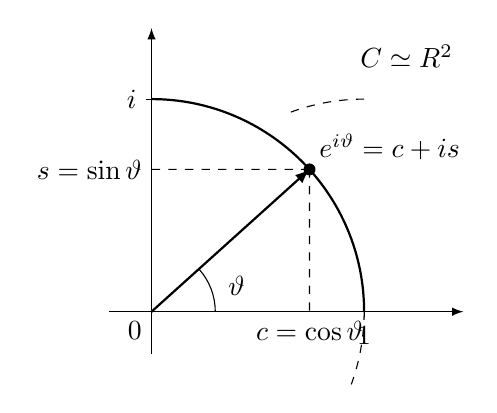
\begin{tikzpicture}[>=latex, scale=1.8]
  % 坐标轴
  \draw[->] (-0.3,0) -- (2.2,0);
  \draw[->] (0,-0.3) -- (0,2.0);
  
  % 原点
  \node[below left] at (0,0) {$0$};
  
  % 单位圆弧 (第 I 象限及两端延展)
  \draw[thick] (1.5,0) arc (0:90:1.5);
  \draw[dashed] (1.5,0) arc (0:-20:1.5);
  \draw[dashed] (1.5,0) ++(90:1.5) arc (90:112:1.5);
  
  % 刻度 1 与 i
  \draw (1.5,-0.04) -- (1.5,0.04) node[below=4pt]{$1$};
  \draw (-0.04,1.5) -- (0.04,1.5) node[left=4pt]{$i$};
  
  % 向量与点 e^{i vartheta}
  \coordinate (Z) at ({1.5*cos(42)}, {1.5*sin(42)});
  \draw[thick, ->] (0,0) -- (Z);
  \fill (Z) circle (1.2pt) node[above right]{$e^{i\vartheta} = c + is$};
  
  % 夹角 vartheta
  \draw (0.45,0) arc (0:42:0.45);
  \node at (0.60,0.18) {$\vartheta$};
  
  % 虚线投影与三角函数值
  \draw[dashed] (Z) -- ({1.5*cos(42)}, 0) node[below]{$c = \cos \vartheta$};
  \draw[dashed] (Z) -- (0, {1.5*sin(42)}) node[left]{$s = \sin \vartheta$};
  
  % 右上角复平面记号
  \node at (1.8, 1.8) {$\mathbb{C} \simeq \mathbb{R}^2$};
\end{tikzpicture}
\end{center}

由于复数的乘法把模相乘并把辐角相加(模 $2\pi$), 且 $e^{i\vartheta}$ 的模为 $1$, 确实可以把 $\mathbb{R}$-线性映射 $\mathbb{C} \longrightarrow \mathbb{C}$, $z \longmapsto e^{i\vartheta} z$, 从而把上述映射 $\varphi \colon \mathbb{R}^2 \longrightarrow \mathbb{R}^2$ 识别为以角度 $\vartheta$ 的旋转.由于 $e^{i\vartheta} = \cos \vartheta + i \sin \vartheta$, 描述矩阵具有形式

\[
R(\vartheta) = \begin{pmatrix} \cos \vartheta & -\sin \vartheta \\ \sin \vartheta & \cos \vartheta \end{pmatrix} \in \mathbb{R}^{2 \times 2}, \qquad 0 \leq \vartheta \leq 2\pi,
\]

并被称为角度 $\vartheta$ 的\emph{旋转矩阵}(\textup{Drehmatrix; R})\index{xuanzhuanjuzhen@旋转矩阵(Drehmatrix; R)}.反过来显然, 每个这样的旋转矩阵在实平面 $\mathbb{R}^2$ 上定义了一个旋转, 从而是一个等距同构.

除旋转之外, $\mathbb{R}^2$ 还有另外的等距同构, 即所谓的反射.$\mathbb{R}$-线性映射 $\varphi \colon \mathbb{R}^2 \longrightarrow \mathbb{R}^2$ 称为一个反射, 如果存在 $\mathbb{R}^2$ 的一个标准正交基 $u_1, u_2$, 使得 $\varphi$ 由

\[
u_1 \longmapsto u_1, \qquad u_2 \longmapsto -u_2
\]

描述.下面的定理~\mtref{thm:7.5.6} 将告诉我们, 旋转和反射是 $\mathbb{R}^2$ 仅有的等距同构.不过我们首先想回到定理~\mtref{thm:7.5.1} 的一般情形, 再作一些推论.

\begin{corollary}\label{cor:7.5.3}
对 $\varphi \in \operatorname{End}_K(V)$, 下列条件等价:
\begin{enumerate}
\item[(i)] $\varphi$ 是一个等距同构;
\item[(ii)] 若 $X$ 是 $V$ 的一个标准正交基, 则 $A_{\varphi, X, X}$ 可逆, 并且成立
\[
(A_{\varphi, X, X})^* = (A_{\varphi, X, X})^{-1};
\]
\item[(iii)] 存在 $V$ 的一个标准正交基 $X$, 使得 $A_{\varphi, X, X}$ 可逆并且成立
\[
(A_{\varphi, X, X})^* = (A_{\varphi, X, X})^{-1}\text{.}
\]
\end{enumerate}
\end{corollary}

\begin{proof}
利用注记~\mtref{rem:7.4.4} 与定理~\mtref{thm:7.5.1} (ii).
\end{proof}

最后容易看出, 推论~\mtref{cor:7.5.3} (ii) 或 (iii) 中的性质 $A^* = A^{-1}$ 也可以用来刻画把 $V$ 的标准正交基变为标准正交基的基变换矩阵.

\begin{theorem}\label{thm:7.5.4}
设 $X$ 是一个标准正交基, $Y$ 是 $V$ 的另一个基.则下列条件等价:
\begin{enumerate}
\item[(i)] $Y$ 是 $V$ 的一个标准正交基;
\item[(ii)] 对基变换矩阵 $A = A_{Y, X}$ 成立 $A^* = A^{-1}$.
\end{enumerate}
\end{theorem}

\begin{proof}
设 $\varphi \colon V \longrightarrow V$ 是把基 $X$ 映到基 $Y$ 的 $K$-线性映射; 此时成立

\[
A_{\varphi, X, X} = A = A_{Y, X}\text{.}
\]

按定理~\mtref{thm:7.5.1} (iv) 或 (v), $Y$ 是一个标准正交基, 当且仅当 $\varphi$ 是一个等距同构, 而按推论~\mtref{cor:7.5.3} 这等价于 $(A_{\varphi, X, X})^* = (A_{\varphi, X, X})^{-1}$, 即等价于 $A^* = A^{-1}$.
\end{proof}

矩阵 $A \in \mathbb{R}^{n \times n}$ 称为正交的, 如果 $\mathbb{R}$-线性映射

\[
\mathbb{R}^n \longrightarrow \mathbb{R}^n, \qquad x \longmapsto A x,
\]

是正交的, 即是一个等距同构.其中借助标准数量积把 $\mathbb{R}^n$ 看作欧几里得向量空间.按推论~\mtref{cor:7.5.3}, 矩阵 $A \in \mathbb{R}^{n \times n}$ 的正交性等价于条件 $A^t = A^{-1}$ 或 $A^t A = E$, 其中 $E \in \mathbb{R}^{n \times n}$ 是单位矩阵.若 $a_1, \ldots, a_n \in \mathbb{R}^n$ 是 $A$ 的列, 则这个条件正是

\[
a_i^t \cdot a_j = \delta_{ij}, \qquad i, j = 1, \ldots, n\text{.}
\]

对 $A$ 的行也可以作相应的考虑.因此矩阵 $A \in \mathbb{R}^{n \times n}$ 正交, 当且仅当其列(或行)组成一个标准正交系, 从而组成 $\mathbb{R}^n$ 的一个标准正交基.

在域 $\mathbb{C}$ 上类似地处理.矩阵 $A \in \mathbb{C}^{n \times n}$ 称为酉的, 如果 $\mathbb{C}$-线性映射

\[
\mathbb{C}^n \longrightarrow \mathbb{C}^n, \qquad x \longmapsto A x,
\]

是酉的, 即是一个等距同构.其中借助标准数量积把 $\mathbb{C}^n$ 看作酉向量空间.按推论~\mtref{cor:7.5.3}, $A \in \mathbb{C}^{n \times n}$ 酉, 当且仅当 $A^* = A^{-1}$ 或 $A^* A = E$ 成立, 而这个条件又等价于 $A$ 的列(或行)组成 $\mathbb{C}^n$ 的一个标准正交基.

由推论~\mtref{cor:7.5.2} 和推论~\mtref{cor:7.5.3} 立即得出, 正交或酉矩阵 $A \in K^{n \times n}$ 组成 $K^{n \times n}$ 中一切可逆矩阵的群 $\mathrm{Gl}(n, K)$ 的一个子群.其中人们把

\[
\mathrm{O}(n) = \bigl\{A \in \mathrm{Gl}(n, \mathbb{R});\; A^t = A^{-1}\bigr\}
\]

称为指标 $n$ 的\emph{正交群}(\textup{orthogonale Gruppe; O(n)})\index{zhengjiaoqun@正交群(orthogonale Gruppe; O(n))}, 把

\[
\mathrm{U}(n) = \bigl\{A \in \mathrm{Gl}(n, \mathbb{C});\; A^* = A^{-1}\bigr\}
\]

称为指标 $n$ 的\emph{酉群}(\textup{unitäre Gruppe; U(n)})\index{youqun@酉群(unitäre Gruppe; U(n))}, 其中可以把 $\mathrm{O}(n)$ 看作 $\mathrm{U}(n)$ 的子群.对 $A \in \mathrm{U}(n)$, $A^* \cdot A$ 是单位矩阵, 所以对每个正交或酉矩阵都得到 $|\det(A)| = 1$.特别地, 可以把

\[
\mathrm{SO}(n) = \bigl\{A \in \mathrm{O}(n);\; \det(A) = 1\bigr\}
\]

看作正交群的子群; 人们把这个群称为\emph{特殊正交群}(\textup{spezielle orthogonale Gruppe; SO(n)})\index{teshuzhengjiaoqun@特殊正交群(spezielle orthogonale Gruppe; SO(n))}.

我们想在 $n = 2$ 的情形更精确地描述正交群 $\mathrm{O}(2)$.上面已经证明, 旋转矩阵

\[
R(\vartheta) = \begin{pmatrix} \cos \vartheta & -\sin \vartheta \\ \sin \vartheta & \cos \vartheta \end{pmatrix} \in \mathbb{R}^{2 \times 2}, \qquad 0 \leq \vartheta < 2\pi,
\]

给出 $\mathbb{R}^2$ 的等距同构, 从而属于 $\mathrm{O}(2)$, 甚至属于子群 $\mathrm{SO}(2)$, 因为总有 $\det(R(\vartheta)) = 1$.我们首先想证明 $\mathrm{SO}(2)$ 不含另外的矩阵.为此考察一个矩阵

\[
A = \begin{pmatrix} \alpha_{11} & \alpha_{12} \\ \alpha_{21} & \alpha_{22} \end{pmatrix} \in \mathrm{O}(2)\text{.}
\]

则关系

\[
\begin{pmatrix} 1 & 0 \\ 0 & 1 \end{pmatrix} = A^t \cdot A = \begin{pmatrix} \alpha_{11}^2 + \alpha_{21}^2 & \alpha_{11}\alpha_{12} + \alpha_{21}\alpha_{22} \\ \alpha_{12}\alpha_{11} + \alpha_{22}\alpha_{21} & \alpha_{12}^2 + \alpha_{22}^2 \end{pmatrix}
\]

给出方程组

\[
\begin{array}{c}
\alpha_{11}^2 + \alpha_{21}^2 = 1, \\
\alpha_{12}^2 + \alpha_{22}^2 = 1, \\
\alpha_{11}\alpha_{12} + \alpha_{21}\alpha_{22} = 0\text{.}
\end{array}
\]

复数

\[
\alpha_{11} + i\alpha_{21}, \qquad \alpha_{22} + i\alpha_{12}
\]

因此绝对值为 $1$.它们的乘积亦然, 于是有

\[
\begin{array}{c}
\bigl(\alpha_{11} + i\alpha_{21}\bigr) \cdot \bigl(\alpha_{22} + i\alpha_{12}\bigr) = \bigl(\alpha_{11}\alpha_{22} - \alpha_{21}\alpha_{12}\bigr) + i\bigl(\alpha_{11}\alpha_{12} + \alpha_{21}\alpha_{22}\bigr) \\
= \alpha_{11}\alpha_{22} - \alpha_{21}\alpha_{12} \\
= \det(A) = \pm 1 \in \mathbb{R}\text{.}
\end{array}
\]

现在利用对绝对值 $1$ 的复数 $z$ 恒有 $z\overline{z} = 1$, 于是在 $\det(A) = 1$ 的情形, 即在 $A \in \mathrm{SO}(2)$ 的情形, 得到

\[
\alpha_{22} + i\alpha_{12} = \overline{\alpha_{11} + i\alpha_{21}} = \alpha_{11} - i\alpha_{21},
\]

从而

\[
\alpha_{22} = \alpha_{11}, \qquad \alpha_{12} = -\alpha_{21}\text{.}
\]

现在我们利用分析中的事实: 由于 $\alpha_{11}^2 + \alpha_{21}^2 = 1$, 存在唯一的角度 $\vartheta$, $0 \leq \vartheta < 2\pi$, 使得

\[
\alpha_{11} + i\alpha_{21} = \cos \vartheta + i \sin \vartheta = e^{i\vartheta},
\]

即

\[
A = \begin{pmatrix} \alpha_{11} & -\alpha_{21} \\ \alpha_{21} & \alpha_{11} \end{pmatrix} = \begin{pmatrix} \cos \vartheta & -\sin \vartheta \\ \sin \vartheta & \cos \vartheta \end{pmatrix} = R(\vartheta)\text{.}
\]

这意味着 $A$ 描述了围绕零点以角度 $\vartheta$ 的旋转.

旋转 $R(\vartheta)$ 的特征多项式计算为

\[
\chi_{R(\vartheta)} = T^2 - 2(\cos \vartheta) T + 1 = (T - e^{i\vartheta})(T - e^{-i\vartheta}),
\]

所以只有在 $\sin \vartheta = 0$, 即 $\vartheta \in \{0, \pi\}$ 的情形才有实零点.于是得到:

\begin{theorem}\label{thm:7.5.5}
$\mathrm{SO}(2)$ 由一切在 $\mathbb{R}^2$ 中引起围绕零点旋转的实 $(2 \times 2)$-矩阵组成, 即

\[
\mathrm{SO}(2) = \bigl\{R(\vartheta);\; 0 \leq \vartheta < 2\pi\bigr\}\text{.}
\]
\end{theorem}

除平凡情形 $R(0) = \mathrm{id}$ 与 $R(\pi) = -\mathrm{id}$ 外, 矩阵 $R(\vartheta)$ 没有实特征值, 从而也不可对角化.

对满足 $\det(A) = -1$ 的矩阵 $A = (\alpha_{ij})_{i, j = 1, 2} \in \mathrm{O}(2)$, 上面的计算以相应方式给出恒等式

\[
\alpha_{22} + i\alpha_{12} = -\overline{(\alpha_{11} + i\alpha_{21})} = -\alpha_{11} + i\alpha_{21},
\]

即

\[
\alpha_{22} = -\alpha_{11}, \qquad \alpha_{12} = \alpha_{21},
\]

所以在这个情形也存在唯一的角度 $\vartheta$, $0 \leq \vartheta < 2\pi$, 使得

\[
A = \begin{pmatrix} \cos \vartheta & \sin \vartheta \\ \sin \vartheta & -\cos \vartheta \end{pmatrix}\text{.}
\]

自然, 这个类型的所有矩阵 $A$ 都属于 $\mathrm{O}(2)$.这样的矩阵的特征多项式计算为 $\chi_A = T^2 - 1$, 所以 $A$ 具有实特征值 $1$ 与 $-1$, 从而可对角化.方程 $A^t = A^{-1}$ 表明, $A$ 描述 $\mathbb{R}^2$ 的一个\emph{正规自同态}(\textup{normaler Endomorphismus})\index{zhengguizitongtai@正规自同态(normaler Endomorphismus)}.按定理~\mtref{thm:7.4.8}, 此时 $\mathbb{R}^2$ 中存在一个由 $A$ 的特征向量组成的标准正交基, 并且看出 $A$ 是一个反射.于是得到:

\begin{theorem}\label{thm:7.5.6}
$\mathrm{O}(2)$ 由一切在 $\mathbb{R}^2$ 中引起旋转或反射的实 $(2 \times 2)$-矩阵组成.更确切地说, 成立

\[
\mathrm{O}(2) = \left\{\begin{pmatrix} \cos \vartheta & -\sin \vartheta \\ \sin \vartheta & \cos \vartheta \end{pmatrix}, \begin{pmatrix} \cos \vartheta & \sin \vartheta \\ \sin \vartheta & -\cos \vartheta \end{pmatrix} \in \mathbb{R}^{2 \times 2};\; 0 \leq \vartheta < 2\pi\right\}\text{.}
\]
\end{theorem}

群 $\mathrm{O}(2)$ 与 $\mathrm{SO}(2)$ 的结构由此完全清楚了.还应该指出(并可以用初等计算验证), $\mathrm{SO}(2)$ 是交换的, 而 $\mathrm{O}(2)$ 不是.

下面我们想推导欧几里得和酉向量空间中一般类型\emph{等距同构的标准形}(\textup{Normalform für orthogonale und unitäre Abbildungen})\index{dengjutonggoudebiaozhunxing@等距同构的标准形(Normalform für orthogonale und unitäre Abbildungen)}.由定理~\mtref{thm:7.5.1} (ii) 特别推出, 每个等距同构都是正规的.相应地, 至少在复数域 $\mathbb{C}$ 上可以应用谱定理~\mtref{thm:7.4.8}.

\begin{theorem}\label{thm:7.5.7}
设 $\varphi \in \operatorname{End}_{\mathbb{C}}(V)$ 是有限维酉 $\mathbb{C}$-向量空间 $V$ 的自同态.则下列条件等价:
\begin{enumerate}
\item[(i)] $\varphi$ 是一个等距同构;
\item[(ii)] 对 $\varphi$ 的每个特征值 $\lambda$ 成立 $|\lambda| = 1$, 并且存在关于 $\varphi$ 的特征向量组成 $V$ 的一个标准正交基.
\end{enumerate}
\end{theorem}

\begin{proof}
首先设 (i) 成立, 即 $\varphi$ 是一个等距同构.则 $\varphi$ 作为保长映射只能有绝对值为 $1$ 的特征值.此外, 由于 $\mathbb{C}$ 代数闭, 特征多项式 $\chi_\varphi$ 完全分裂为一次因式.而且 $\varphi$ 正规.于是由定理~\mtref{thm:7.4.8} 推出存在 $V$ 的一个由关于 $\varphi$ 的特征向量组成的标准正交基 $X$, 即 (ii) 成立.

反之, 若 $X$ 是 $V$ 的一个由关于 $\varphi$ 的特征向量组成的标准正交基, 且所有特征值的绝对值都是 $1$, 则 $X$ 被 $\varphi$ 显然又变换为一个标准正交基.按定理~\mtref{thm:7.5.1}, $\varphi$ 从而是一个等距同构.
\end{proof}

特别地, 有限维酉向量空间的每个等距同构都可对角化.不过对欧几里得向量空间不能指望相应的结果, 正如 $\mathbb{R}^2$ 中围绕零点的旋转的例子所表明的.这里的情形要更复杂一些.

\begin{theorem}\label{thm:7.5.8}
设 $\varphi \in \operatorname{End}_{\mathbb{R}}(V)$ 是有限维欧几里得 $\mathbb{R}$-向量空间 $V$ 的自同态.则下列条件等价:
\begin{enumerate}
\item[(i)] $\varphi$ 是一个等距同构;
\item[(ii)] 存在 $V$ 的一个标准正交基 $X$, 使得 $\varphi$ 关于 $X$ 由一个如下类型的矩阵描述:
\[
A = A_{\varphi, X, X} = \operatorname{Diag}\bigl(E_k, -E_\ell, R(\vartheta_1), \ldots, R(\vartheta_m)\bigr)
\]
\[
= \begin{pmatrix}
E_k & & & & & \\
& -E_\ell & & & & \\
& & R(\vartheta_1) & & & \\
& & & \ddots & & \\
& & & & \ddots & \\
& & & & & R(\vartheta_m)
\end{pmatrix}
\]
其中 $E_k \in \mathbb{R}^{k \times k}$(或 $E_\ell \in \mathbb{R}^{\ell \times \ell}$)是行数和列数为 $k$(或 $\ell$)的单位矩阵, 而 $R(\vartheta_1), \ldots, R(\vartheta_m) \in \mathbb{R}^{2 \times 2}$ 是某个角度 $0 < \vartheta_1 \leq \vartheta_2 \leq \cdots \leq \vartheta_m < \pi$ 的旋转矩阵.
\end{enumerate}

若 $\varphi$ 是一个等距同构, 则 (ii) 中的标准形连同数 $k$, $\ell$, $m$ 与角度 $\vartheta_1, \ldots, \vartheta_m$ 被 $\varphi$ 唯一确定, 并且成立

\[
\chi_\varphi = (T - 1)^k (T + 1)^\ell \prod_{j = 1}^{m} (T - e^{i\vartheta_j})(T - e^{-i\vartheta_j})\text{.}
\]
\end{theorem}

\begin{proof}
首先设 $\varphi$ 是一个等距同构.为推导 (ii) 中断言的标准形, 我们按 $V$ 的维数 $n$ 作归纳.在 $n = 0$ 的情形没有要证的, 设 $n > 0$.我们断言, 此时 $V$ 含有维数为 $1$ 或 $2$ 的 $\varphi$-不可分解线性子空间 $U$.由大定理~\mtref{bigthm:6.5.6} 得出, $V$ 至少有一个 $\varphi$-不变子空间 $U'$, 它在 $\varphi$ 下作为 $\mathbb{R}[T]$-模同构于一个商 $\mathbb{R}[T]/(p^c)$; 其中 $p \in \mathbb{R}[T]$ 是一个素多项式, $c \geq 1$ 是一个幂指数.用 $p^{c-1}$ 相乘定义了一个 $\mathbb{R}[T]$-模同构 $\mathbb{R}[T] \xrightarrow{\sim} p^{c-1}\mathbb{R}[T]$, 并且通过取商定义了一个 $\mathbb{R}[T]$-模同构 $\mathbb{R}[T]/p\mathbb{R}[T] \xrightarrow{\sim} p^{c-1}\mathbb{R}[T]/p^c\mathbb{R}[T]$, 其中可以把 $p^{c-1}\mathbb{R}[T]/p^c\mathbb{R}[T]$ 看作 $\mathbb{R}[T]/(p^c)$ 的 $\mathbb{R}[T]$-子模.于是由注记~\mtref{rem:6.5.2} (i), $U'$ 从而特别地 $V$ 含有一个 $\varphi$-不变的线性子空间 $U$, 它作为 $\mathbb{R}[T]$-模同构于 $\mathbb{R}[T]/(p)$, 从而按定理~\mtref{thm:6.5.4} 或推论~\mtref{cor:6.5.7} 是 $\varphi$-不可分解的, 并且按引理~\mtref{lem:6.5.5} 具有维数 $\operatorname{grad} p$.而 $\mathbb{R}[T]$ 中的素多项式次数为 $1$ 或 $2$, 参见 \ref{sec:5.3} 节习题 3, 于是我们认识到 $U \subset V$ 是维数为 $1$ 或 $2$ 的不可分解 $\varphi$-不变线性子空间.

现在我们考察分解 $V = U \oplus U^{\perp}$, 参见推论~\mtref{cor:7.2.8}, 并且证明, 与 $U$ 一起, 正交补 $U^{\perp}$ 也是 $V$ 的 $\varphi$-不变子空间.为此我们首先注意到, $\varphi$ 作为同构诱导了一个线性映射 $\varphi|_{U} \colon U \longrightarrow U$, 它至少是单射, 但随后由推论~\mtref{cor:2.1.11} 甚至是双射, 从而满足 $\varphi^{-1}(U) = U$.现在设 $y \in U^{\perp}$.则对一切 $x \in U$ 成立

\[
\bigl\langle x, \varphi(y) \bigr\rangle = \bigl\langle \varphi^*(x), y \bigr\rangle = \bigl\langle \varphi^{-1}(x), y \bigr\rangle = 0,
\]

因为正如我们看到的, 与 $x$ 一起 $\varphi^{-1}(x)$ 也属于 $U$.但这意味着 $\varphi(y) \in U^{\perp}$, 于是我们认识到确实 $U^{\perp}$ 是 $V$ 的 $\varphi$-不变子空间.

现在在 $U$ 中选取一个标准正交基 $X'$.在 $\dim_{\mathbb{R}}(U) = 1$ 的情形, $X'$ 只由一个向量组成, 它必然是 $\varphi$ 的特征向量.相应的特征值按定理~\mtref{thm:7.5.1} (iii) 绝对值为 $1$, 即等于 $1$ 或 $-1$.对 $\dim_{\mathbb{R}}(U) = 2$, $X'$ 由两个向量组成, 并且由推论~\mtref{cor:7.5.3} 推出矩阵 $A_{\varphi|_{U}, X', X'}$ 属于 $\mathrm{O}(2)$, 但不可能可对角化, 因为我们曾假定 $U$ 是 $\varphi$-不可分解的.于是由上面关于 $\mathrm{O}(2)$ 中矩阵的描述, 必然有 $A_{\varphi|_{U}, X', X'} = R(\vartheta)$, 其中角度 $\vartheta \neq \pi$, $0 < \vartheta < 2\pi$.必要时通过改变 $X'$ 中向量的顺序(这相当于把角度 $\vartheta$ 换成 $2\pi - \vartheta$), 甚至可以假定 $0 < \vartheta < \pi$.

按归纳假设, $U^{\perp}$ 中存在一个标准正交基 $X''$, 使得 $A_{\varphi|_{U^{\perp}}, X'', X''}$ 具有 (ii) 中描述的形式.于是可以把 $X'$ 与 $X''$ 合成 $V$ 的一个标准正交基 $X$, 并且经过对 $X$ 的基向量适当重新编号, 矩阵 $A_{\varphi, X, X}$ 具有所求的形式.蕴含关系 (i) $\Longrightarrow$ (ii) 得证.反之显然, (ii) 类型的每个矩阵都是正交的, 故在此情形 $\varphi$ 是一个等距同构.

为证唯一性断言, 只需注意: 对等距同构 $\varphi$, 一个如 (ii) 中的描述矩阵 $A$ 的特征多项式计算为

\[
\chi_\varphi = \chi_A = (T - 1)^k (T + 1)^\ell \prod_{j = 1}^{m} (T - e^{i\vartheta_j})(T - e^{-i\vartheta_j})
\]

于是 $\chi_\varphi$ 首先确定 $A$ 中的数 $k$, $\ell$ 与 $m$.由于在成对的复共轭零点 $e^{i\vartheta_j}, e^{-i\vartheta_j}$ 中实部 $\cos \vartheta_j$ 各自相等, 而这个实部唯一确定 $0 < \vartheta_j < \pi$ 范围内的角度, 所以矩阵 $A$ 的整体形状由多项式 $\chi_\varphi$ 确定.
\end{proof}

\aufgaben

除非另外规定, $V$ 恒为有限维欧几里得或酉 $K$-向量空间.

\medskip
\noindent\textbf{习题 1.} 证明: 对 $x, y \in V$, 存在等距同构 $\varphi \in \operatorname{End}_K(V)$ 使得 $\varphi(x) = y$, 当且仅当 $|x| = |y|$ 成立.

\medskip
\noindent\textbf{习题 2.} 对带角度 $0 \leq \vartheta_1 < \vartheta_2 < 2\pi$ 的旋转矩阵 $R(\vartheta_1), R(\vartheta_2) \in \mathbb{R}^{2 \times 2}$ 证明: 它们相似, 当且仅当 $\vartheta_1 + \vartheta_2 = 2\pi$ 成立.(AT 368)

\medskip
\noindent\textbf{习题 3.} 设 $e_1, \ldots, e_n \in \mathbb{R}^n$ 是典范单位向量, 理解为列向量.矩阵 $A \in \mathbb{R}^{n \times n}$ 称为置换矩阵, 如果存在置换 $\pi \in \mathfrak{S}_n$ 使得 $A = E_\pi := (e_{\pi(1)}, \ldots, e_{\pi(n)})$.证明:
\begin{enumerate}
\item[(i)] 每个置换矩阵可逆, 且典范映射 $\sigma \colon \mathfrak{S}_n \longrightarrow \mathrm{Gl}(n, \mathbb{R})$, $\pi \longmapsto E_\pi$ 定义了单射的群同态;
\item[(ii)] 对一切 $\pi \in \mathfrak{S}_n$ 成立 $E_\pi \in \mathrm{O}(n)$;
\item[(iii)] 设 $A = (\alpha_{ij}) \in \mathrm{O}(n)$ 是带系数 $\alpha_{ij} \geq 0$ 的\emph{正交矩阵}(\textup{orthogonale Matrix})\index{zhengjiaojuzhen@正交矩阵(orthogonale Matrix)}.则 $A$ 已经是一个置换矩阵.
\end{enumerate}

\medskip
\noindent\textbf{习题 4.} 设 $A = (\alpha_{ij}) \in \mathrm{O}(n)$ 是下三角形正交矩阵, 即对 $i < j$ 成立 $\alpha_{ij} = 0$.证明: $A$ 甚至是对角矩阵.对矩阵 $A \in \mathrm{U}(n)$ 相应的断言也成立吗? (AT 369)

\medskip
\noindent\textbf{习题 5.} 设 $A, B \in \mathbb{C}^{n \times n}$ 是酉矩阵.证明: $A$ 与 $B$ 相似, 当且仅当它们酉相似, 即存在酉矩阵 $S \in \mathbb{C}^{n \times n}$ 使得 $B = S^{-1} A S$.在域 $K = \mathbb{R}$ 上以"正交"代替"酉"相应的断言也成立吗?

\section{自伴随映射}\index{zibansuide@自伴随的(selbstadjungiert)}\label{sec:7.6}

仍设 $V$ 是带数量积 $\varPhi \colon V \times V \longrightarrow K$ 的有限维 $K$-向量空间, 即一个欧几里得或酉向量空间.

\begin{definition}\label{def:7.6.1}
自同态 $\varphi \in \operatorname{End}_K(V)$ 称为\emph{自伴随的}(\textup{selbstadjungiert})\index{zibansuide@自伴随的(selbstadjungiert)}, 如果成立 $\varphi^* = \varphi$.

矩阵 $A \in K^{n \times n}$ 称为对称的(在 $K = \mathbb{R}$ 的情形)或埃尔米特的(在 $K = \mathbb{C}$ 的情形), 如果成立 $A^* = A$.
\end{definition}

对任意自同态 $\varphi \colon V \longrightarrow V$, 复合 $\varphi \circ \varphi^*$ 是自伴随的, 正如等式

\[
\bigl\langle \varphi \circ \varphi^*(x), y \bigr\rangle = \bigl\langle \varphi^*(x), \varphi^*(y) \bigr\rangle = \bigl\langle x, \varphi \circ \varphi^*(y) \bigr\rangle, \qquad x, y \in V,
\]

所表明的.相应地, 对每个矩阵 $A \in K^{n \times n}$, 乘积 $A A^*$ 是对称或埃尔米特的.此外, $V$ 的每个自伴随自同态都特别地是正规的.借助注记~\mtref{rem:7.4.4} 得到下列自伴随自同态的刻画:

\begin{remark}\label{rem:7.6.2}
设 $X$ 是 $V$ 的一个标准正交基.则对 $\varphi \in \operatorname{End}_K(V)$, 下列条件等价:
\begin{enumerate}
\item[(i)] $\varphi$ 自伴随;
\item[(ii)] $(A_{\varphi, X, X})^* = A_{\varphi, X, X}$, 即 $A_{\varphi, X, X}$ 对称或埃尔米特.
\end{enumerate}
\end{remark}

基于我们对正规自同态的研究, 现在可以作出如下重要观察:

\begin{theorem}\label{thm:7.6.3}
设 $\varphi \in \operatorname{End}_K(V)$ 自伴随.则特征多项式 $\chi_\varphi$ 具有实系数, 并在 $\mathbb{R}[T]$ 中完全分裂为一次因式.特别地, $\varphi$ 只有实特征值.
\end{theorem}

\begin{proof}
首先设 $K = \mathbb{C}$.由推论~\mtref{cor:7.4.7} 得 $\lambda = \overline{\lambda}$, 从而对 $\varphi$ 的一切特征值 $\lambda$ 或 $\chi_\varphi$ 的一切零点成立 $\lambda \in \mathbb{R}$.利用 $\mathbb{C}$ 代数闭这一事实, 我们看到 $\chi_\varphi$ 完全分裂为一次因式, 并且这些因式都是实的.特别地 $\chi_\varphi$ 是一个实多项式.

在 $K = \mathbb{R}$ 的情形选取 $V$ 的一个标准正交基 $X$ 并考察矩阵 $A = A_{\varphi, X, X}$, 其中此时成立 $A^* = A^t = A$; 参见注记~\mtref{rem:7.4.4}.现在把以 $n = \dim_{\mathbb{R}} V$ 的 $\mathbb{C}^n$ 在标准数量积下看作酉向量空间, 则 $A$ 作为对称实矩阵特别地也定义了自伴随自同态

\[
\mathbb{C}^n \longrightarrow \mathbb{C}^n, \qquad x \longmapsto A x,
\]

我们可以像上面那样推出, 相应的特征多项式即 $\chi_A$ 完全分裂为实一次因式.但由于 $\chi_A$ 与 $\chi_\varphi$ 一致, 我们得证.
\end{proof}

因此对自伴随自同态, 我们可以把正规自同态的谱定理~\mtref{thm:7.4.8} 强化为:

\begin{corollary}\label{cor:7.6.4}
对自同态 $\varphi \in \operatorname{End}_K(V)$, 下列条件等价:
\begin{enumerate}
\item[(i)] $\varphi$ 自伴随;
\item[(ii)] $\varphi$ 的所有特征值都是实的, 并且 $V$ 有一个由关于 $\varphi$ 的特征向量组成的标准正交基;
\item[(iii)] 在 $V$ 中存在一个标准正交基 $X$, 使得 $A_{\varphi, X, X}$ 是一个实对角矩阵.
\end{enumerate}
\end{corollary}

\begin{proof}
首先设条件 (i) 成立, 即 $\varphi$ 自伴随.则按定理~\mtref{thm:7.6.3}, 特征多项式 $\chi_\varphi$ 具有实系数并在 $\mathbb{R}$ 上完全分裂为一次因式; 因此所有特征值都是实的.由于 $\varphi$ 特别地正规, 按定理~\mtref{thm:7.4.8} 存在 $V$ 的一个由关于 $\varphi$ 的特征向量组成的标准正交基 $X$, 即条件 (ii) 满足.此外由 (ii) 推出矩阵 $A_{\varphi, X, X}$ 具有对角形式, 其中对角线上的正是 $\varphi$ 的特征值.于是 $A_{\varphi, X, X}$ 是一个实对角矩阵, 正如 (iii) 所断言的.

最后, 若存在 $V$ 的一个标准正交基 $X$, 使得 $A_{\varphi, X, X}$ 是一个实对角矩阵, 则成立

\[
(A_{\varphi, X, X})^* = A_{\varphi, X, X},
\]

并由注记~\mtref{rem:7.4.4} 得 $A_{\varphi^*, X, X} = A_{\varphi, X, X}$, 即 $\varphi^* = \varphi$.条件 (iii) 因此蕴含 (i).
\end{proof}

由于可以把满足 $A = A^*$ 的矩阵 $A \in K^{n \times n}$ 总是解释为 $K^n$(配备标准数量积)的自伴随自同态, 作为直接推论得到:

\begin{corollary}\label{cor:7.6.5}
设 $A \in K^{n \times n}$ 是满足条件 $A^* = A$ 的矩阵, 即一个对称或埃尔米特矩阵.则 $A$ 相似于一个实对角矩阵.特别地成立 $\chi_A \in \mathbb{R}[T]$, 并且这个多项式在 $\mathbb{R}[T]$ 中完全分裂为一次因式.
\end{corollary}

在特殊情形 $K = \mathbb{R}$, 对称矩阵 $A \in \mathbb{R}^{n \times n}$ 从而总是可对角化的, 因此(对 $n \geq 1$)至少有一个(实)特征值.

我们在推论~\mtref{cor:7.6.5} 中还没有利用, 在对称或埃尔米特矩阵 $A$ 与相应的实对角矩阵之间传递相似性的基变换矩阵, 按推论~\mtref{cor:7.6.4} 的构造描述的是标准正交基之间的基变换, 从而按定理~\mtref{thm:7.5.4} 是正交或酉的.我们想利用这一点, 并由此得到所谓的主轴变换定理, 我们将推导它的两个不同版本.\index{zhuzhoubianhuan@主轴变换(Hauptachsentransformation)}

\begin{bigtheorem}\label{bigthm:7.6.6}
设 $A \in K^{n \times n}$ 是满足 $A^* = A$ 的矩阵.则存在正交或酉矩阵 $S \in \mathrm{Gl}(n, K)$, 使得

\[
D = S^{-1} A S = S^* A S = (\overline{S})^t A \overline{\overline{S}}
\]

是一个实对角矩阵.其中与 $S$ 一起, $\overline{S} \in \mathrm{Gl}(n, K)$ 也是正交或酉的, 而 $D$ 的对角线元素恰是 $A$ 的特征值.
\end{bigtheorem}

方程 $D = S^{-1} A S$ 表明, $A$ 作为(自伴随)线性映射 $\mathbb{K}^n \longrightarrow \mathbb{K}^n$ 可以借助由 $S$ 给出的基变换化为对角形.相应地, $D = (\overline{S})^t A \overline{\overline{S}}$ 意味着, 由 $A$ 给出的 sBF 或 HF 可以借助由 $\overline{S}$ 给出的基变换化为对角形.

\begin{bigtheorem}\label{bigthm:7.6.7}
设 $V$ 是带数量积 $\varPhi$ 的欧几里得或酉向量空间, 并且设 $\Psi \colon V \times V \longrightarrow K$ 是 $V$ 上任意 sBF 或 HF.则存在 $V$ 的一个标准正交基 $X$, 使得矩阵 $A_{\varPsi, X}$ 是一个实对角矩阵.
\end{bigtheorem}

\begin{proof}[定理~\mtref{bigthm:7.6.6} 的证明]
我们把 $\mathbb{K}^n$ 连同标准数量积看作欧几里得或酉向量空间.则线性映射

\[
\varphi \colon \mathbb{K}^n \longrightarrow \mathbb{K}^n, \qquad x \longmapsto A x,
\]

自伴随, 因为成立 $A^* = A$; 参见注记~\mtref{rem:7.6.2}.按推论~\mtref{cor:7.6.4}, 因此存在 $\mathbb{K}^n$ 的一个标准正交基 $X$, 使得描述矩阵 $D = A_{\varphi, X, X}$ 是一个实对角矩阵.若 $S = A_{X, E} \in \mathrm{Gl}(n, K)$ 是 $X$ 与 $\mathbb{K}^n$ 的典范基 $E$ 之间的基变换矩阵, 则按推论~\mtref{cor:3.4.5} 得到

\[
D = S^{-1} \cdot A \cdot S\text{.}
\]

由于 $S$ 描述两个标准正交基之间的基变换, 按定理~\mtref{thm:7.5.4}, $S$ 正交或酉, 并成立 $S^* = S^{-1}$.通过取共轭得到 $\overline{S}^* = (\overline{S})^{-1}$, 即 $\overline{S}$ 也是正交或酉的.
\end{proof}

\begin{proof}[定理~\mtref{bigthm:7.6.7} 的证明]
我们从 $V$ 的任意一个标准正交基 $X$ 出发; 参见推论~\mtref{cor:7.2.6}.对属于 $\Psi$ 的矩阵, 按推论~\mtref{cor:7.3.4} 成立 $A_{\varPsi, X} = A_{\varPsi, X}^*$, 并且正如我们在定理~\mtref{bigthm:7.6.6} 中看到的, 存在正交或酉矩阵 $S \in \mathrm{Gl}(n, K)$, 使得 $D = S^t \cdot A_{\varPsi, X} \cdot \overline{S}$ 是一个实对角矩阵.我们可以把 $S$ 看作带 $V$ 的新基 $Y$ 的 $A_{Y, X}$ 型基变换矩阵.按定理~\mtref{thm:7.5.4}, $Y$ 又是一个标准正交基, 并且成立

\[
A_{\varPsi, Y} = S^t \cdot A_{\varPsi, X} \cdot \overline{S} = D,
\]

其中可运用定理~\mtref{thm:7.3.5}.于是 $Y$ 代替 $X$ 满足断言.
\end{proof}

为了阐明主轴变换的几何意义, 例如考察 $\mathbb{R}^2$ 中由方程

\[
41 x_1^2 - 24 x_1 x_2 + 34 x_2^2 = 25
\]

给出的曲线 $C$.以 $x = (x_1, x_2)^t$ 以及

\[
A = \begin{pmatrix} 41 & -12 \\ -12 & 34 \end{pmatrix}
\]

则 $C$ 也可以用方程

\[
x^t \cdot A \cdot x = 25
\]

描述.现在我们运用定理~\mtref{bigthm:7.6.6}, 则存在正交矩阵 $S \in \mathrm{O}(2)$, 使得

\[
D = S^t A S = S^{-1} A S
\]

是一个实对角矩阵, 其中 $D$ 的对角线上正是 $A$ 的特征值.由于 $A$ 的特征多项式具有形式

\[
\chi_A = (T - 25)(T - 50),
\]

我们可以取例如

\[
S^t A S = S^{-1} A S = \begin{pmatrix} 25 & 0 \\ 0 & 50 \end{pmatrix}\text{.}
\]

若 $X = E$ 是 $\mathbb{R}^2$ 的典范基, 则可以把 $S$ 看作带新基 $Y$ 的 $A_{Y, X}$ 型基变换矩阵, 其中按定理~\mtref{thm:7.5.4}, $Y$ 又是一个标准正交基.于是按注记~\mtref{rem:3.4.3} 成立关系

\[
\binom{x_1}{x_2} = S \cdot \binom{y_1}{y_2}
\]

介于关于 $X$ 的坐标 $x_1, x_2$ 与关于 $Y$ 的坐标 $y_1, y_2$ 之间, 所以曲线 $C$ 在新坐标下由方程

\[
25 y_1^2 + 50 y_2^2 = 25
\]

即由

\[
y_1^2 + 2 y_2^2 = 1
\]

描述.特别地我们看到, 这是一个椭圆.此时方程中不再出现交叉项, 这意味着人们已经关于 $C$ 的"主轴"来描述 $C$ 了.

\begin{center}
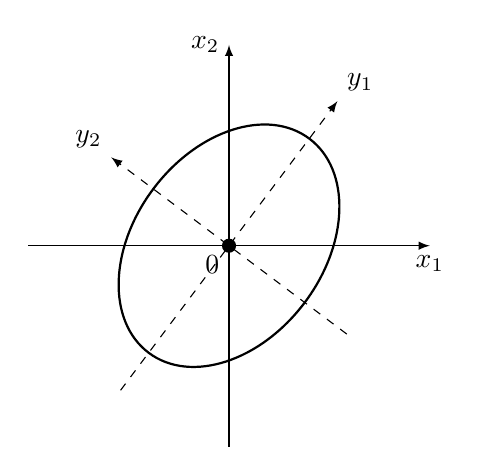
\begin{tikzpicture}[>=latex, scale=1.7]
  \draw[->] (-1.5,0) -- (1.5,0) node[below]{$x_1$};
  \draw[->] (0,-1.5) -- (0,1.5) node[left]{$x_2$};
  \fill (0,0) circle (1.5pt) node[below left]{$0$};
  \draw[rotate=53.13, thick] (0,0) ellipse (1 and 0.7071);
  \begin{scope}[rotate=53.13]
    \draw[->, dashed] (-1.35,0) -- (1.35,0) node[above right]{$y_1$};
    \draw[->, dashed] (0,-1.1) -- (0,1.1) node[above left]{$y_2$};
  \end{scope}
\end{tikzpicture}
\end{center}

为更精确地刻画 $C$, 自然应当显式地确定 $C$ 的主轴, 即标准正交基 $Y$ 和相应的变换矩阵 $S = A_{Y, X}$.这可以如下进行.把

\[
\mathbb{R}^2 \longrightarrow \mathbb{R}^2, \qquad x \longmapsto A x,
\]

看作配备标准数量积的 $\mathbb{R}^2$ 的自伴随自同态, 并确定 $\mathbb{R}^2$ 的一个由关于 $A$ 的特征向量组成的标准正交基 $Y$.为此首先求 $A$ 的特征空间的一个基(通过解相应的线性方程组), 然后按 E.~施密特(Schmidt)对基作正交规范化.在我们的情形这非常简单.

\[
(3, 4)^t, \qquad (-4, 3)^t
\]

是分别属于特征值 $25$ 与 $50$ 的特征向量.规范化后得到

\[
\frac{1}{5}(3, 4)^t, \qquad \frac{1}{5}(-4, 3)^t
\]

作为 $\mathbb{R}^2$ 的标准正交基 $Y$, 以及

\[
S = A_{Y, X} = \frac{1}{5} \begin{pmatrix} 3 & -4 \\ 4 & 3 \end{pmatrix}
\]

作为相应的变换矩阵.其中等距同构

\[
\mathbb{R}^2 \longrightarrow \mathbb{R}^2, \qquad x \longmapsto S x,
\]

可以解释为以大约 $53^{\circ}$ 的角度 $\vartheta$ 的旋转 $R(\vartheta)$.

最后我们还想从主轴变换定理作出一些推论.

\begin{corollary}\label{cor:7.6.8}
对有限维 $K$-向量空间 $V$ 上的 sBF 或 HF $\Psi$, 下列条件等价:
\begin{enumerate}
\item[(i)] $\Psi$ 正定;
\item[(ii)] 存在 $V$ 的一个基 $X$, 使得矩阵 $A_{\varPsi, X}$ 只有正特征值.
\end{enumerate}
\end{corollary}

\begin{proof}
若 $\Psi$ 正定, 则存在关于 $\Psi$ 的 $V$ 的一个标准正交基 $X$.相应的矩阵 $A_{\varPsi, X}$ 此时是单位矩阵.

反之, 设 $X$ 是 $V$ 的一个基, 使得矩阵 $A_{\varPsi, X}$ 只有正特征值.按推论~\mtref{cor:7.3.4} 成立 $A_{\varPsi, X}^* = A_{\varPsi, X}$.由定理~\mtref{bigthm:7.6.6} 于是存在矩阵 $S \in \mathrm{Gl}(n, K)$ 且 $S^* = S^{-1}$, 使得

\[
(\overline{S})^t \cdot A_{\varPsi, X} \cdot \overline{\overline{S}} = S^{-1} A_{\varPsi, X} \cdot S = D
\]

是一个实对角矩阵.其中 $D$ 的对角线元素恰是 $A_{\varPsi, X}$ 的特征值, 从而大于 $0$.若现在把 $\overline{S}$ 解释为带 $V$ 的新基 $Y$ 的 $A_{Y, X}$ 型基变换矩阵, 则成立 $A_{\varPsi, Y} = D$, 并且看出 $\Psi$ 正定.
\end{proof}

\begin{corollary}[Sylvester \emph{惯性定理}\index{guanxingdingli@惯性定理(Sylvester'scher Trägheitssatz)}]\label{cor:7.6.9}\index{guanxingdingli@惯性定理(Sylvester'scher Trägheitssatz)}
设 $\Psi$ 是有限维 $K$-向量空间 $V$ 上的 sBF 或 HF.对 $V$ 的一个基 $X$, 设 $k$ 是 $A_{\varPsi, X}$ 的正特征值个数, $\ell$ 是负特征值个数, $m$ 是消失的特征值个数, 均按重数计数.则成立 $k + \ell + m = \dim_K V$, 并且数 $k$, $\ell$, $m$ 由 $\Psi$ 唯一确定, 特别地与 $X$ 的选取无关.

存在 $V$ 的一个基 $X$, 使得矩阵 $A_{\varPsi, X}$ 具有如下对角形式

\[
A_{\varPsi, X} = \operatorname{Diag}\bigl(\underbrace{1, \ldots, 1}_{k}, \underbrace{-1, \ldots, -1}_{\ell}, \underbrace{0, \ldots, 0}_{m}\bigr),
\]

其中对角线上是 $k$ 个 $1$, $\ell$ 个 $-1$ 和 $m$ 个 $0$.
\end{corollary}

\begin{proof}
我们从 $V$ 的一个基 $X = (x_1, \ldots, x_n)$ 出发, 考察矩阵 $A_{\varPsi, X}$ 及相应的数 $k$, $\ell$, $m$.则按定理~\mtref{bigthm:7.6.6} 结合推论~\mtref{cor:7.3.4}, 存在正交或酉矩阵 $S \in \mathrm{Gl}(n, K)$, 使得 $D = S^t A \overline{S}$ 是一个实对角矩阵; $D$ 的对角线元素恰是 $A$ 的特征值.通过把 $S$ 看作基变换矩阵并用相应的新基代替 $X$, 可以假定

\[
\varPsi(x_i, x_j) = \delta_{ij} \alpha_i
\]

其中 $\alpha_i \in \mathbb{R}$, $i, j = 1, \ldots, n$.此外, 在 $\varPsi(x_i, x_i) \neq 0$ 的情形可以把基向量 $x_i$ 乘以 $|\varPsi(x_i, x_i)|^{-1/2}$, 从而假定 $\alpha_i \in \{1, -1, 0\}$.然后把 $x_i$ 重新编号, 使成立

\[
\alpha_i = \left\{ \begin{array}{l l}
1 & \text{对 } i = 1, \ldots, k \\
-1 & \text{对 } i = k + 1, \ldots, k + \ell \\
0 & \text{对 } i = k + \ell + 1, \ldots, k + \ell + m
\end{array} \right.
\]

则矩阵 $A_{\varPsi, X}$ 具有所断言的形状.

还需证明数 $k$, $\ell$, $m$ 与基 $X$ 的选取无关.设 $X_i$, $i = 1, 2$, 是 $V$ 的两个基, 并设 $k_i$, $\ell_i$, $m_i$ 是相应的数, 其中正如我们刚刚看到的, 可以假定矩阵 $A_{\varPsi, X_i}$ 是实对角矩阵.现在设 $V_i^+ \subset V$ 是由一切满足 $\varPsi(x, x) > 0$ 的 $x \in X_i$ 生成的子空间, $V_i^- \subset V$ 是由一切满足 $\varPsi(x, x) < 0$ 的 $x \in X_i$ 生成的子空间, $V_i^0 \subset V$ 是由一切满足 $\varPsi(x, x) = 0$ 的 $x \in X_i$ 生成的子空间.则对 $i = 1, 2$ 成立

\[
\begin{array}{c}
V = V_i^+ \oplus V_i^- \oplus V_i^0, \\
\dim V_i^+ = k_i, \qquad \dim V_i^- = \ell_i, \qquad \dim V_i^0 = m_i, \\
k_i + \ell_i + m_i = \dim V\text{.}
\end{array}
\]

其中看出

\[
V_1^0 = V_2^0 = \bigl\{x \in V;\; \varPsi(x, y) = 0 \ \text{对一切} \ y \in V\bigr\}
\]

是 $\Psi$ 的"退化空间", 从而成立 $m_1 = m_2$.此外显然有

\[
V_1^+ \cap (V_2^- \oplus V_2^0) = 0,
\]

因为 $\Psi$ 在 $V_1^+$ 上正定而在 $V_2^- \oplus V_2^0$ 上负半定.这意味着

\[
k_1 + \ell_2 + m_2 \leq \dim V
\]

并由 $k_2 + \ell_2 + m_2 = \dim V$ 得到 $k_1 \leq k_2$, 再由对称性理由得 $k_1 = k_2$.于是有

\[
\ell_1 = \dim V - k_i - m_i = \ell_2, \qquad i = 1, 2,
\]

从而得证.
\end{proof}

\aufgaben

除非另外规定, $V$ 恒为有限维欧几里得或酉 $K$-向量空间.

\medskip
\noindent\textbf{习题 1.} 设 $\varphi \in \operatorname{End}_K(V)$ 自伴随.证明: $\varphi$ 恰好具有全部正实特征值, 当且仅当对一切 $x \in V - \{0\}$ 成立 $\langle \varphi(x), x \rangle > 0$.(AT 370)

\medskip
\noindent\textbf{习题 2.} 对正规自同态 $\varphi \in \operatorname{End}_K(V)$ 证明: $\varphi \circ \varphi^*$ 的全部特征值都是实数 $\geq 0$.

\medskip
\noindent\textbf{习题 3.} 对 $A \in \mathbb{R}^{n \times n}$ 证明: $A$ 对称, 当且仅当存在矩阵 $S \in \mathbb{C}^{n \times n}$ 使得 $A = S^t S$.(AT 370)

\medskip
\noindent\textbf{习题 4.} 设 $A \in K^{n \times n}$ 对称或埃尔米特.证明: $A$ 在 $K^n$ 上定义正半定的半双线性形式, 当且仅当 $A$ 具有 $S^* S$ 的形式, 其中 $S \in K^{n \times n}$ 是某个矩阵.

\medskip
\noindent\textbf{习题 5.} 证明: 两个对称或埃尔米特矩阵 $A, B \in K^{n \times n}$ 相似, 当且仅当存在正交或酉矩阵 $S \in \mathrm{Gl}(n, K)$ 使得 $B = S^t A \overline{S}$.


% ===== 附录: 习题训练 =====
% 无编号章在正文中会自动加入目录 (见 titles-setup.tex), 无需重复 \addcontentsline.
\chapter*{习题训练}
\markboth{习题训练}{}
% 附录: 习题训练 (Aufgabentraining)
% 对应源文档 appendix_src.txt (第 1–6822 行).
% 注: 第 1 章解答为完整翻译; 引用第 2–7 章定理处所用标签 (def:2.1.1, thm:2.1.10,
% def:5.2.10, thm:5.2.12 等) 在其对应章节译出前会显示为 "??", 属预期现象.

\section*{总论}

书稿中各个章节的习题提供了将相应呈现的理论运用于具体例子的机会, 从而得以更深入
地加工与理解.有时需要的只是纯粹的例行验证, 但有时也需要稍具创造性的思考.本附录
旨在说明, 如何对习题的解答过程进行有意义的组织安排, 从而使解题更加有效.

在每一章的各个小节中, 我都选取了一些习题, 其解答将在下文以范例的方式加以讨论.
这些习题都带有形如 (AT xyz) 的标注, 表示相应解答的讨论见于习题训练中的第 xyz 页.
自然, 解答一道习题应以最终给出一个尽可能简单的,形式流畅的解答为目标.但至少同样
重要的是事先必须进行的那些思考, 它们导向真正的解题路径.我将这些思考概括在
"策略"这一关键词之下.一般而言, 策略性思考在完成的解答中已不再显现, 但由于其
核心地位, 在随后的讨论中它们往往占据比解答本身更大的篇幅.事实上, 若要以系统的
方式独立地构思一个解答, 或者仅仅是想复现或更好地理解一个现成的解答, 策略性思考
都是不可或缺的.下面将更精确地描述解答一道习题时所需要经历的各个步骤.

\noindent\textbf{起点:} 在一开始, 应从习题文本中提炼出初始情形以及可资利用的前提
条件.此时, 有必要重新回顾所用到的概念构设, 连同在所呈现理论的框架内处理过的相应
性质与结论.

\noindent\textbf{目标:} 在第二步, 应当将所要证明的结论(如有必要)清晰地加以梳理.
尤其应当明确, 具体有哪些论断需要证明.与第一步一样, 在此也有必要再次把所用到的
概念构设以及相应的性质与结论展现在眼前.

\noindent\textbf{策略:} 此时开始规划从起点到目标的实际路线.为了找到一条可行的
路径, 可以首先更仔细地审视初始情形, 并考虑是否存在与所处理的理论相关联的,指向
目标方向的等价或类似的起始条件.另一方面, 也可以进一步分析目标, 提出如下类型的
问题: 目标是否存在等价的描述? 是否有明显的结论可从目标推出? 换言之, 目标是否
存在可能更容易达成的等价版本或弱化形式? 或者是否存在一个适用于完全归纳法的约简
步骤? 简言之, 任何有助于更精确地勘测起点与目标之间"地形"的思考都是有价值的.
在此还尤其应当估量: 目标是否适合直接证明, 抑或更适合通过反证法间接地加以处理.

此外, 考察初始情形中的具体例子通常也极为有用, 无论是几何性质的例子, 还是通过
进一步限制起始前提得到的例子.在此过程中往往能获得有价值的线索, 得知在放宽条件下
如何达成目标, 并由此或许学会在一般情形下如何行事.遗憾的是, 并不存在一个普遍
有效的方法, 能保证将我们从起点带到目标.诚然, 基于上述思考, 通常可以把两点之间
的未知区域大为缩小, 但常常仍剩下一个看似不可逾越的障碍.此时就需要一些创造力,
以发现某个隐藏的突破口.一旦可以说"看见"了一条通向目标的可行路径, 便可进入
下一步, 尝试表述一个完整而数学上精确的解答.

\noindent\textbf{解题路径:} 在这一步, 应当把通过策略性思考所规划的通向目标的路径
以精确的数学形式加以实现.所有那些仅仅有助于发现解题路径,但对实际的求解过程而言
无关紧要的细节在此均被略去.另一方面, 在策略考察的框架内所采用的种种简化, 在这一
步不再被允许.当然, 撰写一份流畅的数学解答需要一定的经验, 而这种经验会随着时间
的推移而逐渐获得.这种经验尤其涉及选择清晰而合用的记号, 以及精心设计论证与所用
结论的先后顺序.这一切都应当在尽可能大的清晰性与简单性的观点下进行.

不过, 倘若在实现预期的解题路径时出乎意料地遭遇不可逾越的困难, 那就别无他法, 只能
回到上一步, 并带着新获得的经验重新进行策略考察.

\noindent\textbf{补充:} 在此要点下, 我们给出关于相应习题问题的若干附加的可选信息,
倘若这对一般读者具有意义的话.就此而言, 这一要点并不属于解答一道习题时所应完成的
常规步骤.

\section*{解法讨论}

下文所讨论的习题解答, 连同相应的策略性思考, 只能被视为范例性的.一般说来, 一个
习题问题存在多种不同,各有道理且地位对等的处理方法.对于导向真正解答的策略性思考,
这一点尤为适用.因此, 我们绝不声称后续的解答讨论是必须遵循的,不可用其他思考替代
的解题方式.

\section*{对应 1.1-1.6: 向量空间}

% 源文档第 118–1392 行.

\subsection*{习题 1.1/1}

\noindent\textbf{起点:} 给定集合 $X$ 的子集 $A, B, C$.

\noindent\textbf{目标:} 需证明下列恒等式:
\[
\text{(i)}\ A \cap (B \cup C) = (A \cap B) \cup (A \cap C),
\]
\[
\text{(ii)}\ A \cup (B \cap C) = (A \cup B) \cap (A \cup C),
\]
\[
\text{(iii)}\ A - (B \cup C) = (A - B) \cap (A - C),
\]
\[
\text{(iv)}\ A - (B \cap C) = (A - B) \cup (A - C)\text{.}
\]

\noindent\textbf{策略:} 我们尚无可用来描述集合的并,交与差之间相互作用的结果.
因此别无他法, 只能依据这些运算的定义, 逐元素地比较各等式左右两侧.为了由此断定
两侧相等, 最清晰的做法是证明: 左侧的每个元素也都包含于右侧, 反之亦然.

\noindent\textbf{解题路径:} 我们从 (i) 开始, 先证包含关系 $\subset$.设
$x \in A \cap (B \cup C)$.则得 $x \in A$ 且 $x \in B \cup C$, 后者意味着
$x \in B$ 或 $x \in C$.对于 $x \in B$, 得 $x \in A \cap B$, 从而
$x \in (A \cap B) \cup (A \cap C)$.相应地, $x \in C$ 同样导致
$x \in (A \cap B) \cup (A \cap C)$.

(i) 的包含关系 $\supset$.设 $x \in (A \cap B) \cup (A \cap C)$.则得
$x \in A \cap B$ 或 $x \in A \cap C$, 但在任何情形下都有 $x \in A$.若
$x \in A \cap B$, 则另外得到 $x \in B$, 从而 $x \in A \cap (B \cup C)$.
相应地, $x \in A \cap C$ 同样给出 $x \in A \cap (B \cup C)$.

(ii) 的包含关系 $\subset$.设 $x \in A \cup (B \cap C)$, 即 $x \in A$ 或
$x \in B \cap C$.对于 $x \in A$, 得 $x \in A \cup B$ 且 $x \in A \cup C$,
从而 $x \in (A \cup B) \cap (A \cup C)$.另一方面, $x \in B \cap C$ 自然给出
$x \in B \subset (A \cup B)$ 且 $x \in C \subset (A \cup C)$, 因此同样有
$x \in (A \cup B) \cap (A \cup C)$.

(ii) 的包含关系 $\supset$.设 $x \in (A \cup B) \cap (A \cup C)$.则特别地
$x \in A \cup B$; 对 $x \in A$, 得 $x \in A \cup (B \cap C)$.但若 $x \notin A$,
则又有 $x \in B$, 相应地 $x \in C$, 从而 $x \in B \cap C \subset A \cup (B \cap C)$.

(iii) 的包含关系 $\subset$.设 $x \in A - (B \cup C)$.则 $x \in A$, 但
$x \notin B \cup C$, 即 $x$ 既不属于 $B$ 也不属于 $C$.于是得
$x \in (A - B) \cap (A - C)$.

(iii) 的包含关系 $\supset$.设 $x \in (A - B) \cap (A - C)$.则 $x \in A - B$
且 $x \in A - C$, 故无论如何 $x \in A$, 并且 $x$ 既不属于 $B$ 也不属于 $C$.
但这意味着 $x \in A - (B \cup C)$.

(iv) 的包含关系 $\subset$.设 $x \in A - (B \cap C)$.则 $x \in A$, 但
$x \notin B \cap C$, 即 $x \notin B$ 或 $x \notin C$.在第一种情形得
$x \in A - B$, 在第二种得 $x \in A - C$; 无论何种情形都有
$x \in (A - B) \cup (A - C)$.

(iv) 的包含关系 $\supset$.设 $x \in (A - B) \cup (A - C)$, 即 $x \in A - B$
或 $x \in A - C$.则无论如何 $x \in A$.在第一种情形有 $x \notin B$, 从而也有
$x \notin B \cap C$.在第二种情形相应地得 $x \notin C$, 从而同样
$x \notin B \cap C$.总而言之得 $x \in A - (B \cap C)$.

\noindent\textbf{补充:} 等式 (iii) 与 (iv) 包含了命题的否定, 例如"$x$ 是 $Y$ 的
元素"这种类型.如人们容易确信的那样, 这对命题 $P$ 与 $Q$ 是按如下原则进行的:
\[
\overline{P \text{ 且 } Q} = \overline{P} \text{ 或 } \overline{Q}, \qquad
\overline{P \text{ 或 } Q} = \overline{P} \text{ 且 } \overline{Q},
\]
其中上横线表示对相应命题的否定.

\subsection*{习题 1.1/5}

\noindent\textbf{起点:} $X$ 是一个集合, $\mathfrak{P}(X)$ 是其幂集, 即 $X$ 的一切
子集的集合.此外给定一个映射 $f \colon X \longrightarrow \mathfrak{P}(X)$.

\noindent\textbf{目标:} 需证明 $f$ 不可能是满射.

\noindent\textbf{策略:} 由于映射 $f$ 并未以任何具体方式给出, 我们猜想所证论断是
建立在某个一般原则之上的.为探究这一原则, 我们考察简单集合 $X$ 的幂集
$\mathfrak{P}(X)$.空集 $X = \emptyset$ 不含任何元素, 而其幂集 $\mathfrak{P}(X)$
恰好含一个元素, 即 $X$.因此, 在这种情况下, 由于 $X$ 与 $\mathfrak{P}(X)$ 的
元素个数之故, 不可能存在满射 $f \colon X \longrightarrow \mathfrak{P}(X)$.
同一个论证也适用于由 $n$ 个不同元素组成的有限集合 $X = \{ x_1, \ldots, x_n \}$.
因为此时 $\mathfrak{P}(X)$ 含有 $n$ 个元素 $\{ x_1 \}, \ldots, \{ x_n \}$, 但此外
还含有其他元素, 例如空集, 故总共至少有 $n + 1$ 个元素.一个计数论证再次表明,
不可能存在满射 $f \colon X \longrightarrow \mathfrak{P}(X)$.

所考察的这些特殊情形提示我们, 在一般情形下不应试图显式地给出一个不属于 $f$ 之像
的 $\mathfrak{P}(X)$ 元素.相反, 应当采用间接方式, 即假设存在一个满射
$f \colon X \longrightarrow \mathfrak{P}(X)$, 并由此导出一个矛盾.刚才考察的有限
集合 $X$ 的例子正是这样运作的.\emph{罗素悖论}(\textup{Paradoxon von Russel})\index{luosubeilun@罗素悖论(Paradoxon von Russel)}为一般做法提供了一些线索.即考虑子集
\[
U = \{ x \in X ; x \notin f(x) \} \subset X.
\]
若 $f$ 是满射, 则存在 $y \in X$ 使得 $U = f(y)$, 而正如我们将看到的, 由此确实
可以导出一个矛盾.

\noindent\textbf{解题路径:} 我们于是假设 $f \colon X \longrightarrow \mathfrak{P}(X)$
是满射, 并考虑子集 $U = \{ x \in X ; x \notin f(x) \} \subset X$.则存在一个元素
$y \in X$ 使得 $U = f(y)$.若 $y \in U$, 则由 $U$ 的定义可知必有
$y \notin f(y) = U$, 这与 $y \in U$ 矛盾.另一方面, 由 $y \notin f(y) = U$ 又可得
$y \in U$, 也构成矛盾.总之, 满射 $f \colon X \longrightarrow \mathfrak{P}(X)$ 的
假设导致矛盾, 于是可知这样的映射不可能存在.

\noindent\textbf{补充:} 顺便提一下, 可以证明: 对含有 $n$ 个不同元素的有限集合 $X$,
其幂集 $\mathfrak{P}(X)$ 恰好有 $2^n$ 个元素.

\subsection*{习题 1.2/4}

\noindent\textbf{起点:} $G$ 是一个群, 带有两个子群 $H_1, H_2 \subset G$; 关于子群
的定义参见定义~\mtref{def:1.2.3}.

\noindent\textbf{目标:} 问的是在何种情形下 $H_1 \cup H_2$ 仍是 $G$ 的子群.对于
$H_1 \subset H_2$, 有 $H_1 \cup H_2 = H_2$; 相应地对于 $H_2 \subset H_1$, 有
$H_1 \cup H_2 = H_1$.因此在这些情形下, $H_1 \cup H_2$ 是 $G$ 的子群.要证明的是,
在所有其他情形下, $H_1 \cup H_2$ 不可能是 $G$ 的子群.

\noindent\textbf{策略:} 若取 $H_1 \cup H_2$ 中两个元素 $a, b$ 的乘积, 那么只要
$a, b$ 同属于 $H_1$ 或同属于 $H_2$, 自然就有 $ab \in H_1 \cup H_2$, 因为此时乘积
$ab$ 又属于 $H_1$ 或 $H_2$.但若取 $H_1 \cup H_2$ 中两个并非同属 $H_1$ 或 $H_2$ 的
元素 $a, b$ 的乘积, 情形就变得关键了, 例如 $a \in H_1 - H_2$ 且 $b \in H_2 - H_1$.
这种情形需要更仔细地考察.

\noindent\textbf{解题路径:} 我们已经看到, 当 $H_1 \subset H_2$ 或 $H_2 \subset H_1$
时, $H_1 \cup H_2$ 出于平凡的理由是 $G$ 的子群.反过来要证明的是, 只要
$H_1 \cup H_2$ 是 $G$ 的子群, 就有 $H_1 \subset H_2$ 或 $H_2 \subset H_1$ 这两个
包含关系之一成立.对这一步我们采用间接方法, 即把 $H_1 \cup H_2$ 设为 $G$ 的子群,
并假设既无 $H_1 \subset H_2$ 也无 $H_2 \subset H_1$, 目标是导出矛盾.于是, 若
$H_1 \not\subset H_2$ 且同时 $H_2 \not\subset H_1$, 则存在元素 $a \in H_1 - H_2$ 与
$b \in H_2 - H_1$.由于我们已假设 $H_1 \cup H_2$ 是 $G$ 的子群, 得
$ab \in H_1 \cup H_2$, 不妨设 $ab \in H_1$.则可从左侧乘以 $a^{-1} \in H_1$, 得到
$b \in H_1$, 与 $b$ 的选取矛盾.但若 $ab \in H_2$, 则从右侧乘以 $b^{-1} \in H_2$
相应地给出 $a \in H_2$, 也与 $a$ 的选取矛盾.因此, 若 $H_1 \cup H_2$ 是 $G$ 的子群,
则假设 $H_1 \not\subset H_2$ 且同时 $H_2 \not\subset H_1$ 是不能成立的.于是如所愿地
得到 $H_1 \subset H_2$ 或 $H_2 \subset H_1$.

\subsection*{习题 1.2/7}

\noindent\textbf{起点:} $G$ 是一个有限交换群; 设 $G = \{ g_1, \ldots, g_n \}$,
其中 $n$ 是 $G$ 的元素个数.

\noindent\textbf{目标:} 需证明
$\displaystyle\prod_{i=1}^{n} g_i^2 = 1$.

\noindent\textbf{策略:} 用展开的记号, 要计算乘积 $g_1 g_1 \cdots g_n g_n$, 并证明它
等于单位元 $1 \in G$.有哪些可能性可以简化这个乘积, 以证明其值为 $1$? 首先我们知道
单位元 $1$ 出现在元素 $g_1, \ldots, g_n$ 之中; 设 $g_1 = 1$.则仍须证明
$g_2 g_2 \cdots g_n g_n = 1$, 但这几乎算不上什么简化.另一方面, 由于 $G$ 是交换的,
我们在计算乘积时可以任意重新安排因子.此外我们记得, 对每个 $g_i \in G$, 在 $G$ 中
存在逆元 $g_j = g_i^{-1}$, 且此时 $g_i g_j = 1$.因此, 在乘积
$g_1^2 \cdots g_n^2$ 内部, 我们可以把元素 $g_i$ 与 $g_j$ 组合起来, 然后把 $g_i g_j$
替换为 $1$.这就是计算乘积 $\prod_{i=1}^{n} g_i^2$ 的关键.

\noindent\textbf{解题路径:} 映射 $\tau \colon G \longrightarrow G,\ g \longmapsto g^{-1}$
是双射, 因为由 $(g^{-1})^{-1} = g$($g \in G$)得 $\tau^2 = \operatorname{id}$.
由于 $G$ 是交换的, 我们可以如下计算:
\[
\prod_{g \in G} g^2 = \prod_{g \in G} g \cdot \prod_{g \in G} \tau(g)
= \prod_{g \in G} g \cdot \prod_{g \in G} g^{-1}
= \prod_{g \in G} (g g^{-1}) = \prod_{g \in G} 1 = 1\text{.}
\]

\subsection*{习题 1.3/2}

\noindent\textbf{起点:} 设 $K$ 是一个由有限多个元素组成的域.对 $n \in \mathbb{N}$
与 $a \in K$, 记 $n \cdot a$ 为 $a$ 与自身的 $n$ 倍和.

\noindent\textbf{目标:} 存在一个自然数 $n > 0$, 使得对所有 $a \in K$ 有
$n \cdot a = 0_K$, 其中 $0_K \in K$ 是零元.若 $n$ 是具有此性质的最小者, 则 $n$ 是
一个素数.

\noindent\textbf{策略:} 对一个元素 $a \in K$, 我们考察其所有倍数
$n \cdot a \in K$, $n \in \mathbb{N}$.这些倍数不可能全都不同, 因为
$\mathbb{N}$ 含有无穷多个元素, 而 $K$ 只含有限多个.因此存在元素
$n', n'' \in \mathbb{N}$, $n' < n''$, 使得 $n' \cdot a = n'' \cdot a$.由此得
\[
n' \cdot a = n'' \cdot a = n' \cdot a + (n'' - n') \cdot a,
\]
从而对 $n = n'' - n' > 0$ 有 $n \cdot a = 0_K$.于是对每个元素 $a \in K$, 都存在
一个自然数 $n > 0$ 使得 $n \cdot a = 0_K$.一般来说, $n$ 会依赖于 $a$ 的选取, 例如
对所有 $n \in \mathbb{N}$ 都有 $n \cdot 0_K = 0_K$, 但 $n \cdot 1_K \neq 0_K$ 当
$n = 1$ 且 $1_K \in K$ 是单位元时.然而, 通过一个技巧, 我们可以使自然数 $n$ 与 $a$
无关.例如, 若 $a_1, a_2 \in K$, 且 $n_1, n_2 \in \mathbb{N} - \{ 0 \}$ 满足
$n_i a_i = 0_K$($i = 1, 2$), 则得
\[
(n_1 n_2) \cdot a_1 = n_2 \cdot (n_1 \cdot a_1) = n_2 \cdot 0_K = 0_K,
\]
\[
(n_1 n_2) \cdot a_2 = n_1 \cdot (n_2 \cdot a_2) = n_1 \cdot 0_K = 0_K\text{.}
\]
如此这般, 我们终于可以找到作为自然数($> 0$)之乘积的 $n$, 使得对 $K$ 的每个元素
$a \in K$(共有限多个)都有 $n \cdot a = 0_K$.

可以想见, 用这种方法却不可能看出这样的 $n$ 在取最小者时是素数.因此我们必须考虑:
寻找满足对所有 $a \in K$ 都有 $n \cdot a = 0_K$ 的自然数 $n > 0$ 这一问题, 是否不能
归结到少数几个元素, 或者最好归结到单个元素 $a \in K$.为此我们注意到, 由
$n \cdot a = 0_K$ 自动推出 $n \cdot (a \cdot b) = (n \cdot a) \cdot b = 0_K$ 对进一步
的元素 $b \in K$ 成立.因此只须考察满足 $n \cdot 1_K = 0_K$ 的自然数 $n > 0$.
这个简化是解决该问题的关键.

\noindent\textbf{解题路径:} 我们上面已经证明, 存在自然数 $n > 0$ 使得
$n \cdot 1_K = 0_K$, 且此时对所有 $a \in K$ 得 $n \cdot a = (n \cdot 1_K) \cdot a = 0_K$.
现在选取具有此性质的最小 $n > 0$.自然有 $n > 1$.若 $n$ 不是素数, 则有分解
$n = n_1 \cdot n_2$, 其中 $n_1, n_2 < n$ 是自然数因子.由此得
\[
\begin{aligned}
0_K &= n \cdot 1_K = (n_1 \cdot n_2) \cdot 1_K = n_1 \cdot (n_2 \cdot 1_K) \\
&= n_1 \cdot \bigl( 1_K \cdot (n_2 \cdot 1_K) \bigr) = (n_1 \cdot 1_K) \cdot (n_2 \cdot 1_K),
\end{aligned}
\]
从而 $n_1 \cdot 1_K = 0_K$ 或 $n_2 \cdot 1_K = 0_K$, 这与 $n$ 的最小性矛盾.故 $n$
必为素数.

\noindent\textbf{补充:} 我们使用了一些诸如对 $n \in \mathbb{N}$,$a \in K$ 形如
$n \cdot a$ 的乘积的结合性之类的计算法则, 这些法则本应加以证明.对
$m, n \in \mathbb{Z}$, $a, b \in K$ 成立下列基本法则:
\[
\begin{array}{rcl}
(m \cdot n) \cdot a = m \cdot (n \cdot a), & & m \cdot (a \cdot b) = (m \cdot a) \cdot b, \\
(m + n) \cdot a = m \cdot a + n \cdot a, & & m \cdot (a + b) = m \cdot a + m \cdot b\text{.}
\end{array}
\]
关于这些法则的证明或多或少是"显然的", 但在更严格的意义上也可以用完全归纳法进行.

这一习题的主题日后还会借助环论的方法再次加以处理; 参见 \ref{sec:5.2} 节末尾关于域的特征的
论述以及那里的习题 9.

\subsection*{习题 1.3/5}

\noindent\textbf{起点:} 要考察的域是 $\mathbb{Q}(\sqrt{2})$, 它由形如
$a + b\sqrt{2}$($a, b \in \mathbb{Q}$)的一切实数组成.根据引理~\mtref{lem:1.3.4}
我们知道 $\sqrt{2} \notin \mathbb{Q}$.特别地, $\mathbb{Q}$ 是
$\mathbb{Q}(\sqrt{2})$ 的真子域.

\noindent\textbf{目标:} 需证明 $\sqrt{3} \notin \mathbb{Q}(\sqrt{2})$.

\noindent\textbf{策略:} 由于我们已经很好地了解了域 $\mathbb{Q}(\sqrt{2})$, 却对其中
不包含的实数知之甚少, 因此宜采用间接论证.故应假设
$\sqrt{3} \in \mathbb{Q}(\sqrt{2})$, 并尝试由此导出矛盾.

\noindent\textbf{解题路径:} 我们假设 $\sqrt{3} \in \mathbb{Q}(\sqrt{2})$.则存在有理数
$a, b \in \mathbb{Q}$ 使得 $a + b\sqrt{2} = \sqrt{3}$, 于是得到
\[
(a + b\sqrt{2})^2 = 3 \quad \text{亦即} \quad a^2 + 2b^2 - 3 = -2ab\sqrt{2}\text{.}
\]
对于 $ab \neq 0$, 我们可以把第二个方程对 $\sqrt{2}$ 求解, 将得到
$\sqrt{2} \in \mathbb{Q}$, 但这根据引理~\mtref{lem:1.3.4} 是被排除的.因此必有
$ab = 0$, 即 $a = 0$ 或 $b = 0$, 且 $a^2 + 2b^2 - 3 = 0$.对 $a = 0$ 得
$2b^2 = 3$.把 $b$ 取为约分后的分数 $\frac{p}{q}$, 其中 $p, q$ 是整数, 则得
$2p^2 = 3q^2$.与引理~\mtref{lem:1.3.4} 的证明一样可推出, $2$ 既是 $q$ 的因子也是
$p$ 的因子, 即分数 $\frac{p}{q}$ 未约分, 与我们的假设矛盾.

剩下要考察 $b = 0$ 的情形, 它归结为方程 $a^2 = 3$.仍把 $a$ 取为约分后的分数
$\frac{p}{q}$, 其中 $p, q$ 是整数.由此得 $p^2 = 3q^2$, 与
引理~\mtref{lem:1.3.4} 的证明一样可推出 $3$ 既是 $p$ 的因子也是 $q$ 的因子, 与我们的
假设矛盾.于是 $\sqrt{3} \in \mathbb{Q}(\sqrt{2})$ 总导致矛盾, 所以 $\sqrt{3}$ 不
可能是 $\mathbb{Q}(\sqrt{2})$ 的元素.

\noindent\textbf{补充:} 严格说来, 我们的论证以简化的形式使用了整数环 $\mathbb{Z}$
中的整除理论, 这将在 \ref{sec:5.2} 节再作详尽的处理.我们确实用到了这样的性质: 像 $2$ 或 $3$
这样的素数是素数元; 为此特别参见定理~\mtref{thm:5.2.12} 之前的论述.$\mathbb{Z}$ 中的
一个素数元 $p$, 参见定义~\mtref{def:5.2.10}, 其特征是: $p$ 整除 $\mathbb{Z}$ 中一个
乘积 $xy$ 当且仅当 $p$ 整除因子 $x$ 与 $y$ 之一.

\subsection*{习题 1.3/11}

\noindent\textbf{起点:} 对 $n, k \in \mathbb{N}$, $n \geq 1$, 考虑集合
\[
X(n, k) = \bigl\{ (a_1, \ldots, a_n) \in \mathbb{N}^n ;\ a_1 + \cdots + a_n = k \bigr\};
\]
记 $\#X(n, k)$ 为元素个数.

\noindent\textbf{目标:} 对 $n, k \in \mathbb{N}$, $n \geq 1$, 需证明下列论断:
\[
A(n, k) \colon \quad \#X(n, k) = \binom{k + n - 1}{n - 1}\text{.}
\]

\noindent\textbf{策略:} 由于我们不能通过明显的计数方式确定 $\#X(n, k)$, 我们尝试用
归纳法证明所求公式.首先显然有
\[
\#X(1, k) = 1 = \binom{k + 1 - 1}{1 - 1}, \qquad
\#X(n, 0) = 1 = \binom{0 + n - 1}{n - 1}
\]
对 $n \geq 1$, $k \geq 0$ 成立, 这些关系可供归纳基础使用.进一步, 对 $X(n+1, k)$ 中
的 $(n+1)$ 元组 $(a_1, \ldots, a_{n+1})$, 我们注意到
$\sum_{i=1}^{n} a_i = k - a_{n+1}$, 从而 $(a_1, \ldots, a_n) \in X(n, k - a_{n+1})$.
由于 $a_{n+1}$ 可以取 $0, \ldots, k$ 各值, 通过对 $X(n+1, k)$ 作相应的分割, 得
关系
\[
\#X(n+1, k) = \#X(n, k) + \#X(n, k-1) + \cdots + \#X(n, 0)\text{.}
\]
这个方程把 $X(n+1, k)$ 中 $(n+1)$ 元组所求的个数归结为若干 $n$ 元组的个数, 因此会
鼓励人们尝试对固定的 $k$ 关于 $n$ 作归纳.对于归纳步骤, 必须把所列的各个个数分别
换成相应的二项式系数, 并且必须验证如下关系:
\[
\binom{k + n}{n} = \binom{k + n - 1}{n - 1} + \cdots + \binom{0 + n - 1}{n - 1}\text{.}
\]
但由于右侧有多个加项, 这并不容易做到.由此我们学到: 应该把 $X(n+1, k)$ 以尽可能
简单的方式加以分割, 例如分为两部分
\[
\begin{array}{l}
X' = \bigl\{ (a_1, \ldots, a_{n+1}) \in X(n+1, k) ;\ a_{n+1} = 0 \bigr\}, \\
X'' = \bigl\{ (a_1, \ldots, a_{n+1}) \in X(n+1, k) ;\ a_{n+1} \geq 1 \bigr\},
\end{array}
\]
其中我们假设 $k \geq 1$.则 $X'$ 与 $X''$ 分别恰好有 $\#X(n, k)$ 与
$\#X(n+1, k-1)$ 个元素, 因为映射
\[
\begin{array}{l}
X' \longrightarrow X(n, k), \quad (a_1, \ldots, a_{n+1}) \longmapsto (a_1, \ldots, a_n), \\
X'' \longrightarrow X(n+1, k-1), \quad (a_1, \ldots, a_{n+1}) \longmapsto (a_1, \ldots, a_{n+1} - 1),
\end{array}
\]
是双射.从而成立等式
\[
\#X(n+1, k) = \#X(n, k) + \#X(n+1, k-1),
\]
我们虽不能把它用于对 $n$ 或 $k$ 的通常归纳步骤, 但或许可用于二重归纳.把满足
$n \geq 1$,$k \geq 0$ 的配对 $(n, k) \in \mathbb{N}^2$ 想象为实平面中的格点, 那么我们
知道所有形如 $(1, k)$ 与 $(n, 0)$ 的点上的所求个数.借助上述公式, 我们可以在点
$(n+1, k)$($k \geq 1$)计算个数, 倘若已知它在点 $(n, k)$ 与 $(n+1, k-1)$ 的值.
几何上可以相信, 通过反复应用这样的步骤, 从形如 $(1, k)$ 与 $(n, 0)$ 的点作为
"归纳基础"出发, 最终可以到达一切有关的格点.为了证明个数 $\#X(n, k)$ 由相应的
二项式系数给出, 我们还需在上述求和分解式中把各个个数替换为相应的二项式系数, 并检验
所得到的方程
\[
\binom{k + n}{n} = \binom{k + n - 1}{n - 1} + \binom{k + n - 1}{n}
\]
对 $n \geq 1$, $k \geq 1$ 成立.但这以乔装的形式正是关于二项式系数的著名公式
\[
\binom{n+1}{i} = \binom{n}{i-1} + \binom{n}{i},
\]
我们在证明二项式公式时已对 $1 \leq i \leq n$ 推导过它.所有这些都鼓励我们把上述思考
扩充为一个完整的解题方案.

\noindent\textbf{解题路径:} 我们用对 $n \geq 1$ 与 $k \geq 0$ 的二重归纳来证明论断
$A(n, k)$.为此需要下列步骤:

(I) $A(n, k)$ 对所有形如 $(1, k)$ 与 $(n, 0)$ 的配对 $(n, k)$ 成立, 这一点我们上面
已经验证过.

(II) 对 $n \geq 1$, $k \geq 1$ 成立如下蕴含式:
\[
\bigl[ A(n, k) \ \text{且}\ A(n+1, k-1) \bigr] \Longrightarrow A(n+1, k)\text{.}
\]
为证明这一蕴含式, 我们使用上面推导出的等式
\[
\#X(n+1, k) = \#X(n, k) + \#X(n+1, k-1)\text{.}
\]
结合 $A(n, k)$ 与 $A(n+1, k-1)$ 以及所提到的二项式系数公式, 得
\[
\#X(n+1, k) = \binom{k + n - 1}{n - 1} + \binom{k + n - 1}{n} = \binom{k + n}{n},
\]
即论断 $A(n+1, k)$.

我们现在还必须考虑, 步骤 (I) 与 (II) 是否足以得到 $A(n, k)$ 对所有 $n \geq 1$ 与
$k \geq 0$ 的成立.为此我们对 $n$ 作归纳, 证明 $A(n, k)$ 对所有 $n \geq 1$ 与任意
$k \geq 0$ 成立.由 (I) 我们知道 $A(1, k)$ 对所有 $k \geq 0$ 成立, 故归纳基础
$n = 1$ 有保证.现设 $n \geq 1$ 任意.我们假设 $A(n, k)$ 对所有 $k \geq 0$ 成立, 并想
由此推出 $A(n+1, k)$ 对所有 $k \geq 0$ 成立.为达此目的, 我们临时用一次对 $k$ 的
归纳.归纳基础 $k = 0$ 由 (I) 是显然的.现设 $k \geq 1$ 且 $A(n+1, k-1)$ 已知成立.
则结合 $A(n, k)$, 由蕴含式 (II) 得到 $A(n+1, k)$ 成立.对 $k$ 的归纳至此完成, 于是
$A(n+1, k)$ 对所有 $k \geq 0$ 成立, 这也完成了对 $n$ 的归纳.这样就证明了 $A(n, k)$
对所有 $n \geq 1$ 与 $k \geq 0$ 成立.

\noindent\textbf{补充:} 我们开始时考察了求和分解式
\[
\#X(n+1, k) = \#X(n, k) + \#X(n, k-1) + \cdots + \#X(n, 0),
\]
但不能用它计算 $\#X(n+1, k)$.由于我们现在知道各个个数都是二项式系数, 由此也就
证明了公式
\[
\binom{k + n}{n} = \binom{k + n - 1}{n - 1} + \cdots + \binom{0 + n - 1}{n - 1}
\]
对 $n \geq 1$, $k \geq 0$ 成立.

\subsection*{习题 1.4/1}

\noindent\textbf{起点:} $U$ 是 $K$-向量空间 $V$ 的一个线性子空间, 即根据
定义~\mtref{def:1.4.2}, $U$ 是 $V$ 中一个非空的,对加法与数乘封闭的子集.特别地,
有 $0 \in U$.

\noindent\textbf{目标:} 我们要刻画所有这样的元素 $a \in V$: 使得连同 $U$,
$a + U = \{ a + u ;\ u \in U \}$ 也是 $V$ 的线性子空间.

\noindent\textbf{策略:} 作为例子, 我们考虑域 $K = \mathbb{R}$ 上的向量空间
$V = \mathbb{R}^3$, 以及 $\mathbb{R}^3$ 中包含原点 $0 \in \mathbb{R}^3$ 的一个平面
$E \subset \mathbb{R}^3$.则 $E$ 是 $\mathbb{R}^3$ 中的线性子空间, 可以把向量
$a \in \mathbb{R}^3$ 的 $a + E$ 想象为把平面 $E$ 沿向量 $a$ 平行移动.对 $a \in E$,
$E$ 被双射地移到自身; 而对 $a \notin E$, 平移沿某个方向发生, 会离开 $E$.此时特别地,
$a + E$ 与 $E$ 不相交, 且 $a + E$ 不再可能是 $\mathbb{R}^3$ 的线性子空间, 因为零向量
$0$ 属于 $E$, 却不属于 $a + E$.

受这一几何例子的启发, 我们也在一般情形下试图证明: 对 $a \in U$, $a + U$ 与 $U$
重合; 而对 $a \notin U$, $a + U$ 不含零向量 $0 \in V$.因此 $a + U$ 是 $V$ 的线性
子空间当且仅当 $a \in U$.

\noindent\textbf{解题路径:} 先设 $a \in U$.由于 $U$ 作为 $V$ 的线性子空间对加法封闭,
得 $a + U \subset U$.由于 $U$ 与 $a$ 一起也包含 $a$, 相应地得 $(-a) + U \subset U$,
两侧同时加上 $a$ 得 $U \subset a + U$.故对 $a \in U$ 有 $a + U = U$, 且 $a + U$ 是
$V$ 的线性子空间.

接下来我们要弄清楚, 对哪些向量 $a \in V$, 集合 $a + U$ 会含有零向量.设
$0 \in a + U$.则存在向量 $b \in U$ 使得 $0 = a + b$.这意味着
$a = -b = (-1) \cdot b \in U$, 因为 $U$ 作为 $V$ 的线性子空间对数乘封闭.于是, 对
$a \notin U$, $a + U$ 不含零向量, 因此不可能是 $V$ 的线性子空间.总而言之我们断定:
$a + U$ 是 $V$ 的线性子空间当且仅当 $a \in U$.

\noindent\textbf{补充:} 另一种做法是, 尝试对 $a + U$ 验证定义~\mtref{def:1.4.2} 中所列
的线性子空间的诸定义性质, 以弄清对哪些 $a \in V$ 这可以做到.原则上这种途径是可行
的, 但最终同样归结为如下本质性认识: 对 $a \in U$ 有 $a + U = U$, 而对 $a \notin U$
有 $0 \notin a + U$.

\subsection*{习题 1.4/5}

\noindent\textbf{起点:} 给定两点 $x, y \in \mathbb{R}^2 - \{ 0 \}$, 它们不共同位于
经过 $0 \in \mathbb{R}^2$ 的同一条直线上; 这意味着 $\mathbb{R}x \neq \mathbb{R}y$,
特别地, 对所有 $\alpha, \beta \in \mathbb{R}^*$ 有 $\alpha x \neq \beta y$.

\noindent\textbf{目标:} $x, y$ 构成 $\mathbb{R}^2$ 的一个生成系, 即
$\mathbb{R}^2 = \langle x, y \rangle$, 其中根据定义--定理~\mtref{std:1.4.5} 有
$\langle x, y \rangle = \{ \alpha x + \beta y ;\ \alpha, \beta \in \mathbb{R} \}$.
此外还需检验, 若把 $\mathbb{R}$ 换成任意域 $K$, 相应的论断是否仍然成立.

\noindent\textbf{策略:} 几何直观已说明应当如何进行.点 $0, x, y$ 与 $x + y$ 张成
一个真正的平行四边形, 因为它们不位于经过 $0$ 的直线上.若 $z \in \mathbb{R}^2$ 非
平凡, 则可过 $z$ 作平行于边 $\overline{0x}$ 与 $\overline{0y}$ 的平行线, 并确定它们
与直线 $\mathbb{R}y$ 和 $\mathbb{R}x$ 的交点.由此得到一个由点 $0, z$ 以及直线
$\mathbb{R}x$ 上一点 $\alpha x$ 与直线 $\mathbb{R}y$ 上一点 $\beta y$ 张成的平行
四边形.于是得 $z = \alpha x + \beta y$, 如所愿.

原则上, 所需的直线及其交点都可以用公式描述或计算, 从而可以这种方式显式地算出常数
$\alpha, \beta \in \mathbb{R}$.但根据点 $x, y, z$ 的位置所需的分情形讨论, 使这一
途径并不吸引人.因此应当考虑如何减少计算量.

\noindent\textbf{解题路径:} 有 $\mathbb{R}^2 = \langle e_1, e_2 \rangle$, 其中
$e_1 = (1, 0)$, $e_2 = (0, 1)$ 是单位向量.若我们能证明 $e_1, e_2 \in \langle x, y
\rangle$, 则由关于生成线性子空间的法则立得
$\mathbb{R}^2 = \langle e_1, e_2 \rangle \subset \langle x, y \rangle \subset
\mathbb{R}^2$, 从而 $\langle x, y \rangle = \mathbb{R}^2$.为证
$e_1 \in \langle x, y \rangle$, 只需证明 $\langle x, y \rangle$ 含有类型
$(\varepsilon, 0)$ 且带有实常数 $\varepsilon \neq 0$ 的一个向量, 因为由此得
$e_1 = \varepsilon^{-1}(\varepsilon, 0) \in \langle x, y \rangle$.若
$x = (x_1, x_2)$ 且 $y = (y_1, y_2)$, 那么为了证明 $e_1 \in \langle x, y \rangle$,
我们最终必须找到常数 $\alpha, \beta \in \mathbb{R}$, 使得对某个
$\varepsilon \in \mathbb{R}^*$ 有 $\alpha x + \beta y = (\varepsilon, 0)$, 即
\[
\alpha x_1 + \beta y_1 \neq 0, \qquad \alpha x_2 + \beta y_2 = 0\text{.}
\]
自然存在不全为 $0$ 的常数 $\alpha, \beta \in \mathbb{R}$ 满足 $\alpha x_2 + \beta y_2
= 0$.此时必有 $\alpha x_1 + \beta y_1 \neq 0$, 因为否则将得 $\alpha x + \beta y = 0$,
即 $\alpha x = -\beta y$, 而这与前提条件--$x$ 和 $y$ 不得共同位于经过 $0$ 的直线
上--相矛盾.于是得 $e_1 \in \langle x, y \rangle$.类似地可以证明
$e_2 \in \langle x, y \rangle$, 然后断定 $\langle x, y \rangle = \mathbb{R}^2$.

最后, 若把 $\mathbb{R}$ 换成任意域 $K$, 具体的几何关联就消失了, 但所进行的计算论证
毫无限制地保持有效, 因此在那种情形下也有 $\langle x, y \rangle = K^2$.

\noindent\textbf{补充:} 解决此题需要运用 \ref{sec:1.4} 节的手段.另一方面, 也可以直接从将在
\ref{sec:1.5} 节处理的关于向量线性无关与向量空间维数的理论得出解答.此外, \ref{sec:4.4} 节中求解线性
方程组的克拉默法则也有帮助, 参见特别是推论~\mtref{cor:4.4.6}, 如果人们想要对给定的
$z \in \mathbb{R}^2$ 确定满足 $\alpha x + \beta y = z$ 的常数 $\alpha, \beta \in
\mathbb{R}$ 的话.

\subsection*{习题 1.5/2}

\noindent\textbf{起点:} $V$ 是带有线性子空间 $U, U' \subset V$ 的 $K$-向量空间, 其中
$U \cap U' = 0$.此外给定 $U$ 中线性无关的向量组 $x_1, \ldots, x_r$ 与 $U'$ 中线性
无关的向量组 $y_1, \ldots, y_s$.

\noindent\textbf{目标:} 向量 $x_1, \ldots, x_r, y_1, \ldots, y_s$ 构成 $V$ 中一个线性
无关的向量组.

\noindent\textbf{策略:} 我们试图按照定义~\mtref{def:1.5.1} 证明向量组
$x_1, \ldots, x_r, y_1, \ldots, y_s$ 的线性无关性, 并考察一个表示零向量的线性组合,
即
\[
\sum_{i=1}^{r} \alpha_i x_i + \sum_{j=1}^{s} \beta_j y_j = 0
\]
其中系数 $\alpha_i, \beta_j \in K$.由 $x_1, \ldots, x_r$ 的线性无关性, 只要我们知道
线性组合 $u = \sum_{i=1}^{r} \alpha_i x_i \in U$ 表示零向量, 就可以推出
$\alpha_1 = \cdots = \alpha_r = 0$.相应地, 若 $v = \sum_{j=1}^{s} \beta_j y_j \in U'$
表示零向量, 则 $\beta_1 = \cdots = \beta_s = 0$.实现等式 $u = 0$ 与 $v = 0$ 的唯一
机会, 在于利用前提 $U \cap U' = 0$.

\noindent\textbf{解题路径:} 设 $\alpha_1, \ldots, \alpha_r, \beta_1, \ldots, \beta_s
\in K$ 满足
\[
\sum_{i=1}^{r} \alpha_i x_i + \sum_{j=1}^{s} \beta_j y_j = 0\text{.}
\]
则考虑向量 $u = \sum_{i=1}^{r} \alpha_i x_i \in U$ 与 $v = \sum_{j=1}^{s} \beta_j y_j
\in U'$.由 $u + v = 0$, 即 $u = -v$ 与 $v = -u$, 得 $u, v \in U \cap U' = 0$,
从而 $u = v = 0$.向量组 $x_1, \ldots, x_r$ 与 $y_1, \ldots, y_s$ 的线性无关性于是
给出: 对所有 $i$ 有 $\alpha_i = 0$, 对所有 $j$ 有 $\beta_j = 0$, 由
定义~\mtref{def:1.5.1} 可知向量组 $x_1, \ldots, x_r, y_1, \ldots, y_s$ 在 $V$ 中线性
无关.

\noindent\textbf{补充:} 这个证明没有前提 $U \cap U' = 0$ 是不会成立的.若确实在
$U \cap U'$ 中存在一个向量 $u \neq 0$, 则它既可表示为 $x_i$ 的非平凡线性组合, 也可
表示为 $y_j$ 的非平凡线性组合, 例如 $u = \sum_{i=1}^{r} \alpha_i x_i$ 与
$v = \sum_{j=1}^{s} \beta_j y_j$, 则
\[
\sum_{i=1}^{r} \alpha_i x_i + \sum_{j=1}^{s} (-\beta_j) y_j = 0
\]
是 $0$ 的一个非平凡线性组合.即向量组 $x_1, \ldots, x_r, y_1, \ldots, y_s$ 将线性
相关.

\subsection*{习题 1.5/3}

\noindent\textbf{起点:} 要考察的是可变 $n \in \mathbb{N}$ 的 $\mathbb{R}$-向量空间
$\mathbb{R}^n$.

\noindent\textbf{目标:} 问的是哪些指数 $n \in \mathbb{N}$ 具有如下性质: 存在一个向量
序列 $a_1, a_2, \ldots \in \mathbb{R}^n$, 使得该序列任意两个向量都构成一个线性无关
的向量组.

\noindent\textbf{策略:} 我们已经看到 $\dim \mathbb{R}^n = n$.因此根据
推论~\mtref{cor:1.5.12}, 在 $\mathbb{R}^n$ 中只对 $n \geq 2$ 才可能存在长度为 $2$ 的
线性无关向量组.另一方面, 一个向量空间中两个向量线性相关, 当且仅当其中一个是另一个
的倍数.从而几何上可以相信: 两点 $x, y \in \mathbb{R}^n$ 恰好当 $x$ 与 $y$ 不位于
经过 $0$ 的直线上时, 才给出 $\mathbb{R}^n$ 中一个线性无关的向量组.由于在
$\mathbb{R}^2$ 中可以给出无穷多条不同的直线, 在 $\mathbb{R}^2$ 中应当也存在一个具有
所要求性质的无穷向量序列.把 $\mathbb{R}^2$ 视为 $\mathbb{R}^n$($n \geq 2$)的线性
子空间, 我们读得: 我们的问题对所有 $n \geq 2$ 可解, 而对 $n < 2$ 不可解, 正如我们
开头所见.

\noindent\textbf{解题路径:} 我们已经论证过, 只有在 $n \geq 2$ 时, $\mathbb{R}^n$ 中才
至多可能存在一个向量序列, 使得其中任意两个向量都构成线性无关的向量组.为了给出这样
的序列 $a_1, a_2, \ldots \in \mathbb{R}^2$, 我们取 $a_i = (i, 1)$, 并断言对 $i \neq j$,
向量 $a_i, a_j$ 线性无关.事实上, 设 $\alpha, \beta \in \mathbb{R}$ 满足
$\alpha a_i + \beta a_j = 0$, 即
\[
\alpha i + \beta j = 0, \qquad \alpha + \beta = 0\text{.}
\]
则得 $\alpha = -\beta$, 从而 $\beta \cdot (j - i) = 0$.由 $j - i \neq 0$ 得
$\beta = 0$, 进而 $\alpha = 0$.故向量 $a_i, a_j$ 在 $\mathbb{R}^2$ 中线性无关.
同样的论证也适用于 $n \geq 2$ 时的 $\mathbb{R}^n$, 只要把 $\mathbb{R}^2$ 等同于线性
子空间 $\{ (\alpha_1, \ldots, \alpha_n) \in \mathbb{R}^n ;\ \alpha_3 = \cdots = \alpha_n
= 0 \} \subset \mathbb{R}^n$.

\noindent\textbf{补充:} 这个例子非常漂亮地表明: 一个向量组的某些(真)部分组的线性
无关性, 一般说来不能说明整个向量组的线性无关性.但请注意, 一个向量组线性无关当且仅
当它的每个有限部分组都线性无关.我们在 \ref{sec:1.5} 节中对无穷向量组认识到了这一刻画, 但它
对有限向量组也平凡地成立.

\subsection*{习题 1.5/8}

\noindent\textbf{起点:} 对域 $K$ 与 $n \in \mathbb{N}$, 考虑 $K$-向量空间 $K^n$, 以及
如下形式的子集
\[
U = \left\{ (\alpha_1, \ldots, \alpha_n) \in K^n ;\ \sum_{i=1}^{n} \alpha_i \gamma_i = 0 \right\} \subset K^n
\]
其中 $\gamma_1, \ldots, \gamma_n \in K$ 是某些常数.

\noindent\textbf{目标:} $U$ 是 $K^n$ 的线性子空间, 需计算其相应的维数.

\noindent\textbf{策略:} 依据定义~\mtref{def:1.4.2} 验证 $U$ 的线性子空间诸性质没有任何
困难.但我们必须考虑如何确定 $U$ 的维数, 并从特殊情形 $n = 0$ 开始.此时
$U = K^0 = 0$, 从而 $\dim_K U = 0$.其次, 对 $n = 1$, $U$ 由
$U = \{ \alpha_1 \in K^1 ;\ \alpha_1 \gamma_1 = 0 \}$ 给出.而 $\alpha_1 \gamma_1 = 0$
当且仅当 $\alpha_1 = 0$ 或 $\gamma_1 = 0$.因此对 $\gamma_1 = 0$ 有 $U = K^1$, 对
$\gamma_1 \neq 0$ 有 $U = 0$, 相应地 $\dim_K U = \dim_K K^1 = 1$ 或
$\dim_K U = 0 = \dim_K K^1 - 1$.我们还应当考察特殊情形 $n = 2$, 即
\[
U = \left\{ (\alpha_1, \alpha_2) \in K^2 ;\ \alpha_1 \gamma_1 + \alpha_2 \gamma_2 = 0 \right\}\text{.}
\]
对于 $(\gamma_1, \gamma_2) = (0, 0)$, 同样可以看出 $U = K^2$, 从而
$\dim_K U = \dim_K K^2 = 2$.但若假设 $(\gamma_1, \gamma_2) \neq (0, 0)$, 例如
$\gamma_2 \neq 0$, 则我们还可以如下描述 $U$:
\[
U = \left\{ (\alpha_1, \alpha_2) \in K^2 ;\ \alpha_2 = -\gamma_2^{-1} \gamma_1 \cdot \alpha_1 \right\} = K \cdot (1, -\gamma_2^{-1} \gamma_1)\text{.}
\]
向量 $(1, -\gamma_2^{-1} \gamma_1)$ 于是构成 $U$ 的一个基, 我们得到
$\dim_K U = 1 = \dim_K K^2 - 1$.基于这些预考察, 可以设想一般情形的如下结果: 若
$\gamma_1 = \cdots = \gamma_n = 0$, 则 $\dim_K U = n$; 否则 $\dim_K U = n - 1$.

\noindent\textbf{解题路径:} 为证明 $U$ 是 $K^n$ 的线性子空间, 我们验证
定义~\mtref{def:1.4.2} 的条件.显然 $0 \in U$, 从而 $U \neq \emptyset$.再设
$a = (\alpha_1, \ldots, \alpha_n)$ 与 $b = (\beta_1, \ldots, \beta_n)$ 是 $U$ 的元素,
即 $\sum_{i=1}^{n} \alpha_i \gamma_i = 0$ 且 $\sum_{i=1}^{n} \beta_i \gamma_i = 0$, 则得
$\sum_{i=1}^{n} (\alpha_i + \beta_i) \gamma_i = 0$, 即 $a + b \in U$.此外, 对
$\alpha \in K$ 也有 $\sum_{i=1}^{n} \alpha \alpha_i \gamma_i = 0$, 从而
$\alpha \cdot a \in U$.于是 $U$ 被确认为 $K^n$ 的线性子空间.

为确定 $\dim_K U$, 我们首先注意到: 在平凡情形 $\gamma_1 = \cdots = \gamma_n = 0$ 中,
线性子空间 $U$ 与 $K^n$ 重合, 得到 $\dim_K U = \dim_K K^n = n$.现设 $\gamma_i$ 中至少
有一个不为 $0$, 例如 $\gamma_n \neq 0$, 这特别要求 $n \geq 1$.则
\[
U = \left\{ (\alpha_1, \ldots, \alpha_n) \in K^n ;\ \alpha_n = -\gamma_n^{-1} \sum_{i=1}^{n-1} \alpha_i \gamma_i \right\},
\]
我们看到, 对 $U$ 的元素 $(\alpha_1, \ldots, \alpha_n)$, 分量 $\alpha_1, \ldots,
\alpha_{n-1} \in K$ 不受任何条件约束, 而 $\alpha_n$ 由这些前几个分量唯一确定.设
$e'_1, \ldots, e'_{n-1} \in K^{n-1}$ 是标准单位向量, 则因此存在唯一确定的向量
$a_1, \ldots, a_{n-1} \in U$, 其前 $n-1$ 个分量分别与 $e'_1, \ldots, e'_{n-1}$ 的分量
一致.我们断言 $a_1, \ldots, a_{n-1}$ 是 $U$ 的一个基, 从而
$\dim_K U = n - 1$.事实上, 考察一个方程 $\sum_{i=1}^{n-1} \lambda_i a_i = 0$, 系数
$\lambda_i \in K$, 则删去下标为 $n$ 的分量后得方程 $\sum_{i=1}^{n-1} \lambda_i e'_i = 0$.
由于 $e'_1, \ldots, e'_{n-1}$ 构成 $K^{n-1}$ 的一个基, 所有 $\lambda_i$ 都平凡, 特别地,
向量 $a_1, \ldots, a_{n-1}$ 构成一个线性无关的向量组.以类似的方式可以证明这些向量
生成 $U$, 从而构成 $U$ 的一个基.为此我们考察任意向量 $a \in U$.删去最后一个分量后,
由它得到一个向量 $a' \in K^{n-1}$, 我们可以找到常数 $\lambda_1, \ldots, \lambda_{n-1}
\in K$, 使得 $a' = \sum_{i=1}^{n-1} \lambda_i e'_i$.则 $a$ 与
$\sum_{i=1}^{n-1} \lambda_i a_i$ 是 $U$ 中两个前 $n-1$ 个分量一致的向量.由于下标为 $n$
的分量由前 $n-1$ 个分量唯一确定, 得 $a = \sum_{i=1}^{n-1} \lambda_i a_i$.因此
$a_1, \ldots, a_{n-1}$ 构成 $U$ 的一个生成系, 从而构成一个基, 我们断定
$\dim_K U = n - 1$.

\noindent\textbf{补充:} 对 $\gamma_1, \ldots, \gamma_n \in K$ 可以考察映射
\[
f \colon K^n \longrightarrow K^1, \quad (\alpha_1, \ldots, \alpha_n) \longmapsto \sum_{i=1}^{n} \alpha_i \gamma_i\text{.}
\]
这是一个线性映射, 参见定义~\mtref{def:2.1.1}, 这意味着 $f$ 保持加法与数乘, 即对所有
$a, b \in K^n$ 与 $\alpha \in K$ 有
\[
f(a + b) = f(a) + f(b), \qquad f(\alpha \cdot a) = \alpha \cdot f(a)\text{.}
\]
此外, $U$ 与 $f^{-1}(0)$ 一致, 即所谓 $f$ 的核, 它由于 $f$ 的线性性始终是 $K^n$ 的
线性子空间.同样容易由 $f$ 的线性性看出, 像 $f(K^n)$ 是 $K^1$ 的线性子空间.对线性
映射现在成立所谓维数公式, 在我们的情形即
$\dim_K K^n = \dim_K f^{-1}(0) + \dim_K f(K^n)$, 我们将在定理~\mtref{thm:2.1.10} 中作
一般证明.由于
\[
f(K^n) = \begin{cases} 0 & \text{若 } \gamma_1 = \cdots = \gamma_n = 0, \\ K^1 & \text{否则,} \end{cases}
\]
我们可以轻易读出: 若 $\gamma_i$ 都平凡, 则 $\dim_K U = n$; 若 $\gamma_i$ 至少有一个
非零, 则 $\dim_K U = n - 1$.

\subsection*{习题 1.6/4}

\noindent\textbf{起点:} 给定 $K$-向量空间 $V$ 的线性子空间 $U_1, U_2, U_3$.

\noindent\textbf{目标:} 需证明如下维数公式:
\[
\dim_K U_1 + \dim_K U_2 + \dim_K U_3 = \dim_K (U_1 + U_2 + U_3) + \dim_K \bigl( (U_1 + U_2) \cap U_3 \bigr) + \dim_K (U_1 \cap U_2)\text{.}
\]

\noindent\textbf{策略:} 在定理~\mtref{thm:1.6.5} 中, 对两个线性子空间 $U, U' \subset V$
证明了维数公式
\[
\dim_K U + \dim_K U' = \dim_K (U + U') + \dim_K (U \cap U')\text{.}
\]
自然要把此公式应用于 $U = U_1 + U_2$ 与 $U' = U_3$, 何况在要证的公式右侧出现了项
$\dim_K ((U_1 + U_2) \cap U_3)$.

\noindent\textbf{解题路径:} 我们把维数公式定理~\mtref{thm:1.6.5} 应用于 $V$ 的线性子
空间 $U_1 + U_2$ 与 $U_3$, 得到
\[
\dim_K (U_1 + U_2) + \dim_K U_3 = \dim_K (U_1 + U_2 + U_3) + \dim_K \bigl( (U_1 + U_2) \cap U_3 \bigr)\text{.}
\]
再把维数公式应用于 $U_1$ 与 $U_2$, 得
\[
\dim_K U_1 + \dim_K U_2 = \dim_K (U_1 + U_2) + \dim_K (U_1 \cap U_2),
\]
于是总共
\[
\dim_K U_1 + \dim_K U_2 + \dim_K U_3 = \dim_K (U_1 + U_2 + U_3) + \dim_K \bigl( (U_1 + U_2) \cap U_3 \bigr) + \dim_K (U_1 \cap U_2),
\]
这就是所要证明的.

\noindent\textbf{补充:} 用完全归纳法可以类似地推导出对有限多个线性子空间
$U_1, \ldots, U_n \subset V$ 的维数公式.

\subsection*{习题 1.6/8}

\noindent\textbf{起点:} 给定一个有限维 $K$-向量空间 $V$ 及其线性子空间 $U \subset V$.
设 $n = \dim_K V$, $s = \dim_K U$.

\noindent\textbf{目标:} 需考虑: 对哪些 $r \in \mathbb{N}$, 以及在 $U$ 与 $V$ 的维数
满足何种条件之下, 存在 $U$ 在 $V$ 中的补空间 $U_1, \ldots, U_r$, 使其和
$\sum_{i=1}^{r} U_i$ 是直和.最优的是一个必要且充分的条件.

\noindent\textbf{策略:} 对 $r = 0$ 无须证明, 因为此时没有涉及 $U$ 的补空间, 且空和
总是取值 $0$.因此值得关注的只有个数 $r > 0$.其中 $r = 1$ 的情形是平凡的, 但
$r = 2$ 的情形已不能一眼看穿.我们由此学到: 参数 $r$ 不应处于中心位置, 而应服从
其余参数 $n$ 与 $s$.

为作进一步的定向, 我们看一个例子, 即 $\mathbb{R}$-向量空间 $V = \mathbb{R}^3$ 与
线性子空间(平面)$U = \{ (\alpha_1, \alpha_2, \alpha_3) \in \mathbb{R}^3 ;\ \alpha_3 = 0 \}$.
由于 $\dim U = 2$, 每个不包含于 $U$ 中的向量 $a = (\alpha_1, \alpha_2, \alpha_3) \in
\mathbb{R}^3$, 即满足 $\alpha_3 \neq 0$ 的向量, 都张成 $U$ 在 $V$ 中的一个补空间.
这样的向量 $a$ 有无限多个, 事实上甚至有不计其数的,不位于 $U$ 中的类型
$\mathbb{R} \cdot a \subset \mathbb{R}^3$ 的直线, 它们定义 $U$ 的补空间.若对
$i = 1, \ldots, r$, $\mathbb{R} \cdot a_i$ 都是这样的补空间, 且和
$\sum_{i=1}^{r} \mathbb{R} \cdot a_i$ 是直和, 则向量 $a_1, \ldots, a_r$ 构成一个线性
无关的向量组, 其中由 $\dim \mathbb{R}^3 = 3$ 必然推出 $r \leq 3$.另一方面, 也确实
存在一个不在 $U$ 中,从而张成 $U$ 在 $\mathbb{R}^3$ 中的补空间的线性无关向量组
$a_1, a_2, a_3 \in \mathbb{R}^3$, 即向量
\[
(0, 0, 1), \qquad (1, 0, 1), \qquad (1, 1, 1)\text{.}
\]
上述考察在一般情形下也把我们引向一个至少是必要的条件: 若存在 $U$ 在 $V$ 中的补空间
$U_1, \ldots, U_r$, 其和 $\sum_{k=1}^{r} U_k \subset V$ 是直和, 则由
定理~\mtref{thm:1.6.4} 对有限多个被加项的推广得
\[
\sum_{k=1}^{r} \dim_K U_k \leq \dim_K V = n\text{.}
\]
又由定理~\mtref{thm:1.6.4} 得, 对所有 $k$ 有 $\dim_K U_k = \dim_K V - \dim_K U = n - s$,
于是给出必要条件 $r \cdot (n - s) \leq n$.在我们上面的例子中, $n = 3$, $s = 2$, 条件
于是取形式 $r \leq 3$, 并且如我们所看到的, 它尤其也是充分的.

为在一般情形下也找到我们问题的充分条件, 我们首先来考虑, 可以用什么方式构造 $U$ 在
$V$ 中的不同补空间.我们首先选取 $U$ 在 $V$ 中的任意一个补空间 $U'$.与
定理~\mtref{thm:1.6.4} 的证明一样, 它可以如下构造: 选取 $U$ 的一个基 $x_1, \ldots, x_s$,
并用元素 $y_1, \ldots, y_t$($t = n - s$)把它扩充为 $V$ 的一个基.则
$U' = \bigoplus_{j=1}^{t} K y_j$ 是 $U$ 在 $V$ 中的一个补空间.若我们现在想改变 $U'$,
那么有意义的做法是改变 $U'$ 的生成元 $y_j$, 而且--为了有把握离开 $U'$--用 $U$ 中
的元素来改变.因此我们选取元素 $a_1, \ldots, a_t \in U$, 并检验向量
$y_1 + a_1, \ldots, y_t + a_t$ 是否也张成一个补空间.为此只需检验这些元素连同
$x_1, \ldots, x_s$ 构成一个线性无关的向量组, 从而构成 $V$ 的一个基.于是设
$\lambda_1, \ldots, \lambda_s, \lambda'_1, \ldots, \lambda'_t \in K$ 满足
\[
\sum_{i=1}^{s} \lambda_i x_i + \sum_{j=1}^{t} \lambda'_j (y_j + a_j) = \left( \sum_{i=1}^{s} \lambda_i x_i + \sum_{j=1}^{t} \lambda'_j a_j \right) + \sum_{j=1}^{t} \lambda'_j y_j = 0\text{.}
\]
则 $\sum_{i=1}^{s} \lambda_i x_i + \sum_{j=1}^{t} \lambda'_j a_j \in U$ 且
$\sum_{j=1}^{t} \lambda'_j y_j \in U'$.由于和 $U + U'$ 是直和, 这两个元素必都为零.
由此得 $\lambda'_1, \ldots, \lambda'_t = 0$, 进而 $\lambda_1, \ldots, \lambda_s = 0$, 即
$U'' = \sum_{j=1}^{t} K \cdot (y_j + a_j)$ 确实是 $U$ 在 $V$ 中的又一个补空间, 而且当
向量 $a_1, \ldots, a_t$ 中至少有一个非平凡时, 它不同于 $U'$.我们想检验: 和
$U' + U''$ 能否是直和, 即向量 $y_1, \ldots, y_t, y_1 + a_1, \ldots, y_t + a_t$ 是否
构成一个线性无关的向量组.因此设 $\lambda'_1, \ldots, \lambda'_t, \lambda''_1, \ldots,
\lambda''_t \in K$, 使得
\[
\sum_{j=1}^{t} \lambda'_j y_j + \sum_{j=1}^{t} \lambda''_j (y_j + a_j) = \sum_{j=1}^{t} \lambda''_j a_j + \sum_{j=1}^{t} (\lambda'_j + \lambda''_j) y_j = 0\text{.}
\]
则 $\sum_{j=1}^{t} \lambda''_j a_j \in U$ 且 $\sum_{j=1}^{t} (\lambda'_j + \lambda''_j) y_j
\in U'$, 而由于和 $U + U'$ 是直和, 两个元素又必为零.于是可以对所有 $j$ 推出
$\lambda'_j + \lambda''_j = 0$, 但只有当向量 $a_1, \ldots, a_t$ 在 $U$ 中构成一个线性
无关的向量组时, 才能对所有 $j$ 推出 $\lambda''_j = 0$.后者例如在 $t \leq s$ 且对
$j = 1, \ldots, t$ 取 $a_j = x_j$ 时成立.这是关键性观察, 它将向我们表明: 条件
$r \cdot (n - s) \leq n$ 对我们的问题的求解确实也是充分的.

\noindent\textbf{解题路径:} 我们要证明: 存在 $U$ 在 $V$ 中的补空间 $U_1, \ldots, U_r$,
其和是直和, 当且仅当 $r(n - s) \leq n$.正如我们所见, 这一条件是必要的.若
$U_1, \ldots, U_r$ 确是如此的补空间, 则由定理~\mtref{thm:1.6.4} 对所有 $k = 1, \ldots, r$
有 $\dim_K U_k = n - s$, 于是由推论~\mtref{cor:1.5.14} 与定理~\mtref{thm:1.6.4} 对有限多
个被加项的推广得
\[
r(n - s) = \sum_{k=1}^{r} \dim_K U_k = \dim_K \bigoplus_{k=1}^{r} U_k \leq \dim_K V = n\text{.}
\]
反之, 现设 $r \in \mathbb{N}$ 满足 $r(n - s) \leq n$.则得 $(r - 1)(n - s) \leq s$, 即
$(r - 1)t \leq s$, 其中 $t = n - s$.此外我们可以假定 $r \geq 2$, 因为要证的论断在其
余情形下是平凡的.现在我们在 $U$ 中选取一个由 $(r - 1)t$ 个向量组成的线性无关向量组,
写成形式
\[
x_{jk}, \qquad j = 1, \ldots, t, \qquad k = 2, \ldots, r;
\]
这是可能的, 因为 $(r - 1)t \leq s = \dim_K U$.又设 $U_1$ 是 $U$ 在 $V$ 中的任意一个
补空间, $y_1, \ldots, y_t$ 是 $U_1$ 的一个基, 其中我们利用 $t = n - s = \dim_K U_1$.
然后令
\[
U_k = \sum_{j=1}^{t} K \cdot (y_j + x_{jk}) \quad \text{对} \ k = 2, \ldots, r\text{.}
\]
由于显然对所有 $j = 1, \ldots, t$ 与 $k = 2, \ldots, r$ 有 $y_j \in U + U_k$, 得
$U + U_k = V$ 对所有 $k$ 成立, 并且借助推论~\mtref{cor:1.6.6} 从维数理由得知和
$U + U_k$ 是直和.于是除 $U_1$ 之外, $U_2, \ldots, U_r$ 也是 $U$ 在 $V$ 中的补空间.
为证明和 $\sum_{k=1}^{r} U_k$ 是直和, 我们考察一个线性组合
\[
\sum_{j=1}^{t} \lambda_j y_j + \sum_{k=2}^{r} \sum_{j=1}^{t} \lambda_{jk} (y_j + x_{jk}) = 0,
\]
系数 $\lambda_j, \lambda_{jk} \in K$.这个方程也可以写成形式
\[
\left( \sum_{j=1}^{t} \lambda_j y_j + \sum_{k=2}^{r} \sum_{j=1}^{t} \lambda_{jk} y_j \right) + \left( \sum_{k=2}^{r} \sum_{j=1}^{t} \lambda_{jk} x_{jk} \right) = 0,
\]
其中左边括号中的表达式属于 $U_1$, 右边的属于 $U$.由于和 $V = U + U_1$ 是直和, 两个
表达式必都为零.由 $x_{jk}$ 的线性无关性推出所有系数 $\lambda_{jk}$ 为零, 由 $y_j$ 的
线性无关性推出系数 $\lambda_j$ 也为零.于是 $y_j$($j = 1, \ldots, t$)连同向量
$y_j + x_{jk}$($j = 1, \ldots, t$, $k = 2, \ldots, r$)构成 $V$ 中一个线性无关的向量
组, 由此得和 $\sum_{k=1}^{r} U_k$ 在 $V$ 中是直和.这样就证明了条件 $r(n - s) \leq n$
对解决我们的问题不仅必要而且充分.

\noindent\textbf{补充:} 若 $x_1, \ldots, x_s$ 是 $U$ 的一个基, 则在上面的证明中还可以
更具体地选取向量 $x_{jk}$, 即令
\[
x_{jk} = x_{j + (k-2) t}, \qquad j = 1, \ldots, t, \qquad k = 2, \ldots, r\text{.}
\]

\section*{对应 2.1-2.3: 线性映射}

\subsection*{习题 2.1/2}

\noindent\textbf{起点:} 在不同的情形 (i)--(iv) 中, 要考虑的是若干显式给出的向量 $a_i \in \mathbb{R}^4$ 以及 $b_i \in \mathbb{R}^3$($i = 1, 2, 3, 4$ 或 $i = 1, 2, 3$).

\noindent\textbf{目标:} 问是否存在 $\mathbb{R}$-线性映射 $\mathbb{R}^4 \longrightarrow \mathbb{R}^3$, 使它对所有 $i$ 都把 $a_i$ 映到 $b_i$.

\noindent\textbf{策略:} 我们在定理~\mtref{thm:2.1.7} 及其相应的证明中学到, 可以通过线性扩张来定义一个 $\mathbb{R}$-线性映射 $f \colon \mathbb{R}^4 \longrightarrow \mathbb{R}^3$: 考虑 $\mathbb{R}^4$ 的一个基 $a_1, \ldots, a_4$, 并任意指定它们的像 $b_1, \ldots, b_4 \in \mathbb{R}^3$.所得的 $\mathbb{R}$-线性映射由 $f(a_i) = b_i$, $i = 1, 2, 3, 4$, 唯一确定.因此在相应的情形中, 如果向量 $a_1, \ldots, a_4$ 线性无关, 那么它们构成 $\mathbb{R}^4$ 的一个基, 并且总存在唯一确定的 $\mathbb{R}$-线性映射 $f \colon \mathbb{R}^4 \longrightarrow \mathbb{R}^3$, 把 $a_i$ 映到相应的向量 $b_i \in \mathbb{R}^3$.如果只给出向量 $a_1, a_2, a_3 \in \mathbb{R}^4$ 且它们构成一个线性无关组, 那么可以类似地处理.借助定理~\mtref{thm:1.5.8} 用一个向量 $a$ 把这个组扩充为 $\mathbb{R}^4$ 的一个基, 就可以找到 $\mathbb{R}$-线性映射 $f \colon \mathbb{R}^4 \longrightarrow \mathbb{R}^3$, 把 $a_1, a_2, a_3$ 映到 $b_1, b_2, b_3$, 并把 $a$ 映到另一个任意选取的向量 $b \in \mathbb{R}^3$(例如 $b = 0$).这时映射 $f$ 自然依赖于 $b$ 的选取, 因而不再由 $a_1, a_2, a_3$ 到 $b_1, b_2, b_3$ 的像唯一确定.

如果向量 $a_1, \ldots, a_4 \in \mathbb{R}^4$ 构成一个线性相关组, 那该怎么办? 这时可以考虑由 $a_1, \ldots, a_4$ 生成的线性子空间 $U = \langle a_1, \ldots, a_4 \rangle \subset \mathbb{R}^4$, 并把组 $a_1, \ldots, a_4$ 缩减为 $U$ 的一个基.例如, 如果 $a_1, a_2, a_3$ 构成 $U$ 的一个基, 那么正如我们所看到的, 总存在 $\mathbb{R}$-线性映射 $f \colon \mathbb{R}^4 \longrightarrow \mathbb{R}^3$, 把 $a_1, a_2, a_3$ 映到 $b_1, b_2, b_3$.按定理~\mtref{thm:2.1.7} 这个映射在 $U$ 上唯一确定.然后通过把 $a_4$ 表示成 $a_1, a_2, a_3$ 的线性组合, 来检验是否也有 $f(a_4) = b_4$.在第一种情形存在所希望类型的 $\mathbb{R}$-线性映射 $\mathbb{R}^4 \longrightarrow \mathbb{R}^3$, 在第二种情形则不存在.

\noindent\textbf{解题路径:} (i) 我们断言, 向量组
\[
a_1 = (1, 1, 0, 0), \quad a_2 = (1, 1, 1, 0), \quad a_3 = (0, 1, 1, 1), \quad a_4 = (0, 0, 1, 1)
\]
线性无关, 从而构成 $\mathbb{R}^4$ 的一个基.为验证这一点, 我们考虑系数 $\lambda_i \in \mathbb{R}$ 的方程 $\sum_{i = 1}^{4} \lambda_i a_i = 0$, 即按分量的写法考虑下列方程组:
\[
\begin{array}{l}
\lambda_1 \cdot 1 + \lambda_2 \cdot 1 + \lambda_3 \cdot 0 + \lambda_4 \cdot 0 = 0\\
\lambda_1 \cdot 1 + \lambda_2 \cdot 1 + \lambda_3 \cdot 1 + \lambda_4 \cdot 0 = 0\\
\lambda_1 \cdot 0 + \lambda_2 \cdot 1 + \lambda_3 \cdot 1 + \lambda_4 \cdot 1 = 0\\
\lambda_1 \cdot 0 + \lambda_2 \cdot 0 + \lambda_3 \cdot 1 + \lambda_4 \cdot 1 = 0
\end{array}
\]
前两个方程给出 $\lambda_3 = 0$, 后两个给出 $\lambda_2 = 0$.于是又得 $\lambda_1 = 0$ 和 $\lambda_4 = 0$, 我们看到向量 $a_1, a_2, a_3, a_4$ 构成一个线性无关组, 从而是 $\mathbb{R}^4$ 的一个基.于是由定理~\mtref{thm:2.1.7} 读出, 存在 $\mathbb{R}$-线性映射 $\mathbb{R}^4 \longrightarrow \mathbb{R}^3$, 把 $a_1, a_2, a_3, a_4$ 映到预先给定的向量 $b_1, b_2, b_3, b_4 \in \mathbb{R}^3$.

(ii) 我们断言, 这里的向量组
\[
a_1 = (0, 1, 1, 1), \quad a_2 = (1, 0, 1, 1), \quad a_3 = (1, 1, 0, 1)
\]
也线性无关.同样考虑系数 $\lambda_i \in \mathbb{R}$ 的方程 $\sum_{i = 1}^{3} \lambda_i a_i = 0$, 即下列方程组:
\[
\begin{array}{l}
\lambda_1 \cdot 0 + \lambda_2 \cdot 1 + \lambda_3 \cdot 1 = 0\\
\lambda_1 \cdot 1 + \lambda_2 \cdot 0 + \lambda_3 \cdot 1 = 0\\
\lambda_1 \cdot 1 + \lambda_2 \cdot 1 + \lambda_3 \cdot 0 = 0\\
\lambda_1 \cdot 1 + \lambda_2 \cdot 1 + \lambda_3 \cdot 1 = 0
\end{array}
\]
第一个和第四个方程给出 $\lambda_1 = 0$, 第二个和第四个给出 $\lambda_2 = 0$.于是也有 $\lambda_3 = 0$, 我们看到 $a_1, a_2, a_3$ 构成一个线性无关组.把这个组扩充为 $\mathbb{R}^4$ 的一个基, 再次由定理~\mtref{thm:2.1.7} 看到, 存在 $\mathbb{R}$-线性映射 $f \colon \mathbb{R}^4 \longrightarrow \mathbb{R}^3$, 把 $a_1, a_2, a_3$ 映到预先给定的向量 $b_1, b_2, b_3 \in \mathbb{R}^3$.再次应用定理~\mtref{thm:2.1.7} 得到, 只有 $f$ 到线性子空间 $\langle a_1, a_2, a_3 \rangle \subset V$ 上的限制是唯一确定的.

(iii) 我们再次检验向量组
\[
a_1 = (0, 1, 1, 1), \qquad a_2 = (1, 0, 1, 1), \qquad a_3 = (1, 1, 0, 1), \qquad a_4 = (-1, 1, 0, 0)
\]
是否线性无关, 并设系数 $\lambda_i \in \mathbb{R}$ 的方程 $\sum_{i = 1}^{4} \lambda_i a_i = 0$.因此要解下列方程组:
\[
\begin{array}{l}
\lambda_1 \cdot 0 + \lambda_2 \cdot 1 + \lambda_3 \cdot 1 - \lambda_4 \cdot 1 = 0\\
\lambda_1 \cdot 1 + \lambda_2 \cdot 0 + \lambda_3 \cdot 1 + \lambda_4 \cdot 1 = 0\\
\lambda_1 \cdot 1 + \lambda_2 \cdot 1 + \lambda_3 \cdot 0 + \lambda_4 \cdot 0 = 0\\
\lambda_1 \cdot 1 + \lambda_2 \cdot 1 + \lambda_3 \cdot 1 + \lambda_4 \cdot 0 = 0
\end{array}
\]
第一个和第四个方程给出 $\lambda_1 + \lambda_4 = 0$, 第二个和第四个给出 $\lambda_2 - \lambda_4 = 0$, 第三个和第四个给出 $\lambda_3 = 0$.特别地, 基于这些关系, 值
\[
\lambda_1 = 1, \qquad \lambda_2 = -1, \qquad \lambda_3 = 0, \qquad \lambda_4 = -1
\]
是可能的, 而代入上述方程表明, 这的确是方程组的一个解.于是 $a_1 - a_2 - a_4 = 0$, 即 $a_4 = a_1 - a_2$, 向量组 $a_1, a_2, a_3, a_4$ 线性相关.

如我们在 (ii) 中所见, 向量 $a_1, a_2, a_3$ 构成一个线性无关组, 且存在 $\mathbb{R}$-线性映射 $f \colon \mathbb{R}^4 \longrightarrow \mathbb{R}^3$ 满足 $f(a_i) = b_i$, $i = 1, 2, 3$, 其中 $f$ 到线性子空间 $\langle a_1, a_2, a_3 \rangle \subset V$ 上的限制唯一确定.此外有
\[
f(a_4) = f(a_1 - a_2) = f(a_1) - f(a_2) = b_1 - b_2 = (-1, -1, 2) \neq b_4\text{.}
\]
在这种情形下, 因此不存在满足 $f(a_i) = b_i$, $i = 1, 2, 3, 4$, 的 $\mathbb{R}$-线性映射 $f \colon \mathbb{R}^4 \longrightarrow \mathbb{R}^3$.

(iv) 在向量
\[
a_1 = (0, 1, 1, 1), \qquad a_2 = (1, 0, 1, 1), \qquad a_3 = (1, 1, 0, 1), \qquad a_4 = (0, 2, 0, 1)
\]
的情形, 我们同样考虑系数 $\lambda_i \in \mathbb{R}$ 的方程 $\sum_{i = 1}^{4} \lambda_i a_i = 0$, 它把我们引到下列方程组:
\[
\begin{array}{l}
\lambda_1 \cdot 0 + \lambda_2 \cdot 1 + \lambda_3 \cdot 1 + \lambda_4 \cdot 0 = 0\\
\lambda_1 \cdot 1 + \lambda_2 \cdot 0 + \lambda_3 \cdot 1 + \lambda_4 \cdot 2 = 0\\
\lambda_1 \cdot 1 + \lambda_2 \cdot 1 + \lambda_3 \cdot 0 + \lambda_4 \cdot 0 = 0\\
\lambda_1 \cdot 1 + \lambda_2 \cdot 1 + \lambda_3 \cdot 1 + \lambda_4 \cdot 1 = 0
\end{array}
\]
第一个和第四个方程给出 $\lambda_1 + \lambda_4 = 0$, 第二个和第四个给出 $\lambda_2 - \lambda_4 = 0$, 第三个和第四个给出 $\lambda_3 + \lambda_4 = 0$.基于这些关系, 值
\[
\lambda_1 = 1, \qquad \lambda_2 = -1, \qquad \lambda_3 = 1, \qquad \lambda_4 = -1
\]
是可能的, 而代入上述方程表明, 这的确是一个解.于是 $a_4 = a_1 - a_2 + a_3$.与 (ii) 一样, 向量 $a_1, a_2, a_3$ 线性无关, 与 (iii) 一样, 存在 $\mathbb{R}$-线性映射 $f \colon \mathbb{R}^4 \longrightarrow \mathbb{R}^3$ 满足 $f(a_i) = b_i$, $i = 1, 2, 3$.现在有
\[
f(a_4) = f(a_1 - a_2 + a_3) = f(a_1) - f(a_2) + f(a_3) = b_1 - b_2 + b_3 = (2, 0, 4) = b_4\text{.}
\]
因此 $f \colon \mathbb{R}^4 \longrightarrow \mathbb{R}^3$ 正如所希望的那样, 是满足 $f(a_i) = b_i$, $i = 1, 2, 3, 4$, 的 $\mathbb{R}$-线性映射.

\noindent\textbf{补充:} 在确定系数 $\lambda_i$ 时所考虑的方程组是所谓的线性方程组.这些方程组及其相关的实用求解方法的理论, 将在后面的 \ref{sec:3.5} 节中详细讨论.

\subsection*{习题 2.1/5}

\noindent\textbf{起点:} 给定 $K$-向量空间 $V$ 的一个自同态 $f \colon V \longrightarrow V$, 满足 $f^2 = f$.

\noindent\textbf{目标:} 要证明 $V = \ker f \oplus \operatorname{im} f$, 即线性子空间的和 $\ker f + \operatorname{im} f \subset V$ 是直和并等于 $V$.

\noindent\textbf{策略:} 对每个自同态 $f \colon V \longrightarrow V$ 都可以把和 $\ker f + \operatorname{im} f$ 作为 $V$ 的线性子空间来构造.这个和一般不是直的, 例如由定理~\mtref{thm:2.1.7} (ii) 定义的,带典范单位向量 $e_1, e_2 \in K^2$ 的自同态
\[
f \colon K^2 \longrightarrow K^2, \qquad e_1 \longmapsto 0, \qquad e_2 \longmapsto e_1,
\]
就表明了这一点; 这里 $f^2 = 0 \neq f$, 且 $\ker f = \operatorname{im} f = K e_1$.我们由此学到, 条件 $f^2 = f$ 对和 $\ker f + \operatorname{im} f$ 的直和性将是关键的.此外, 如果已认识到这个和是直的, 那么由定理~\mtref{thm:1.6.4} 与维数公式(定理~\mtref{thm:2.1.10})得
\[
\dim_K(\ker f \oplus \operatorname{im} f) = \dim_K(\ker f) + \dim_K(\operatorname{im} f) = \dim_K V\text{.}
\]
因此如果 $V$ 有限维, 我们就能借助推论~\mtref{cor:1.5.14} (ii) 直接读出 $V = \ker f \oplus \operatorname{im} f$.

于是要说明的是, 和 $\ker f + \operatorname{im} f \subset V$ 是直的, 即 $\ker f \cap \operatorname{im} f = 0$.这可以例行地验证.设 $x \in \ker f \cap \operatorname{im} f$.则一方面 $f(x) = 0$, 另一方面存在向量 $x' \in V$ 使 $f(x') = x$.于是 $f^2(x') = 0$, 又因 $f^2 = f$ 还有 $x = f(x') = f^2(x') = 0$, 即 $\ker f \cap \operatorname{im} f = 0$.

还须证明 $V = \ker f + \operatorname{im} f$, 而不假定 $V$ 有限维.为此考虑向量 $x \in V$, 尝试找到向量 $x'' \in \operatorname{im} f$, 使得 $x - x'' \in \ker f$.这里一个显然的候选是 $x'' = f(x)$.

\noindent\textbf{解题路径:} 我们已经证明和 $\ker f + \operatorname{im} f \subset V$ 是直的.为看出 $\ker f + \operatorname{im} f = V$, 选取 $x \in V$.则得
\[
f(x - f(x)) = f(x) - f^2(x) = f(x) - f(x) = 0,
\]
即 $x - f(x) \in \ker f$, 从而 $x \in \ker f + \operatorname{im} f$, 这正是要证明的.

\noindent\textbf{补充:} 如我们所认识到的, 条件 $f^2 = f$ 对关系式 $V = \ker f \oplus \operatorname{im} f$ 是充分的.但它不是必要的, 因为对向量空间 $V \neq 0$, 总存在满足 $f^2 \neq f$ 的自同构 $f \colon V \longrightarrow V$.若 $f$ 是这样的自同构, 则 $\ker f = 0$ 且 $\operatorname{im} f = V$, 从而平凡地有 $V = \ker f \oplus \operatorname{im} f$.

\subsection*{习题 2.1/8}

\noindent\textbf{起点:} 给定有限维 $K$-向量空间之间的 $K$-线性映射 $V_1 \xrightarrow{f} V_2 \xrightarrow{g} V_3$.

\noindent\textbf{目标:} 要证明 $\operatorname{rg} f + \operatorname{rg} g \leq \operatorname{rg}(g \circ f) + \dim_K V_2$, 其中\emph{线性映射的秩}(\textup{Rang einer linearen Abbildung})\index{xianxingyingshedezhi@线性映射的秩(Rang einer linearen Abbildung)}定义为相应像的维数.

\noindent\textbf{策略:} 由于在待证不等式中出现 $K$-线性映射 $f$, $g$ 以及 $g \circ f$ 的秩, 我们尝试使用维数公式(定理~\mtref{thm:2.1.10})的相应版本, 即
\[
\begin{array}{l}
\dim_K V_1 = \dim_K(\ker f) + \operatorname{rg} f,\\
\dim_K V_2 = \dim_K(\ker g) + \operatorname{rg} g,\\
\dim_K V_1 = \dim_K(\ker(g \circ f)) + \operatorname{rg}(g \circ f).
\end{array}
\]
于是得
\[
\operatorname{rg} f + \operatorname{rg} g = \dim_K V_1 + \dim_K V_2 - \dim_K(\ker f) - \dim_K(\ker g),
\]
再利用第三个公式得
\[
\operatorname{rg} f + \operatorname{rg} g = \dim_K(\ker(g \circ f)) + \operatorname{rg}(g \circ f) + \dim_K V_2 - \dim_K(\ker f) - \dim_K(\ker g).
\]
因此我们可以通过证明
\[
\dim_K(\ker(g \circ f)) \leq \dim_K(\ker f) + \dim_K(\ker g)
\]
来达到目标.为获得这个不等式的思路, 我们先弄清所涉及的向量空间.$\ker f$ 和 $\ker(g \circ f)$ 是 $V_1$ 的线性子空间, 且 $\ker f \subset \ker(g \circ f) \subset V_1$, 这容易验证.此外 $\ker g$ 是 $V_2$ 的线性子空间, 确切地说有 $f(\ker(g \circ f)) \subset \ker g \subset V_2$.这鼓励我们考察由 $f$ 诱导的线性映射
\[
\tilde{f} \colon \ker(g \circ f) \longrightarrow \ker g,
\]
其核与 $\ker f$ 一致, 并对它应用维数公式(定理~\mtref{thm:2.1.10}).这的确给出
\[
\dim_K(\ker(g \circ f)) = \dim_K(\ker \tilde{f}) + \dim_K(\operatorname{im} \tilde{f}) \leq \dim_K(\ker f) + \dim_K(\ker g),
\]
即所希望的,为达到目标还须证明的不等式.

上述途径看起来有点复杂, 我们自问是否也能用稍简单些的论证达到目标.我们论证的一个要点是, 把线性子空间 $\operatorname{im} \tilde{f} \subset V_2$ 换成 $\ker g$, 从而使用不等式 $\dim_K(\operatorname{im} \tilde{f}) \leq \dim_K(\ker g)$.其中更确切地有
\[
\operatorname{im} \tilde{f} = \ker g \cap f(V_1),
\]
这容易看出.这使我们想到, 不用给定的映射 $f$ 和 $g$, 而用 $K$-线性映射
\[
V_1 \xrightarrow{f'} f(V_1) \xrightarrow{g'} V_3,
\]
其中 $f'$ 和 $g'$ 分别由 $f$ 和 $g$ 通过把 $V_2$ 换成 $f(V_1)$ 的限制得到.这一做法事实上导致一个更简单的解, 我们马上就会看到.

\noindent\textbf{解题路径:} 我们于是把 $V_2$ 限制到 $f(V_1)$, 考虑所得的 $K$-线性映射 $V_1 \xrightarrow{f'} f(V_1) \xrightarrow{g'} V_3$.然后把维数公式(定理~\mtref{thm:2.1.10})应用于 $g'$, 得
\[
\begin{array}{r l}
& \operatorname{rg} f = \dim_K f(V_1) = \dim_K(\ker g') + \dim_K(\operatorname{im} g')\\
& \qquad = \dim_K\bigl(\ker g \cap f(V_1)\bigr) + \operatorname{rg}(g \circ f)\\
& \qquad \leq \dim_K(\ker g) + \operatorname{rg}(g \circ f).
\end{array}
\]
再利用按 $g$ 的维数公式给出的 $\dim_K(\ker g) = \dim_K V_2 - \operatorname{rg} g$, 即得所希望的不等式 $\operatorname{rg} f + \operatorname{rg} g \leq \operatorname{rg}(g \circ f) + \dim_K V_2$.

\subsection*{习题 2.2/4}

\noindent\textbf{起点:} 给定一个带子集 $A \subset V$ 的 $K$-向量空间.

\noindent\textbf{目标:} 要考虑满足 $A \subset B$ 的子集 $B \subset V$, 使得由
\[
x \sim_B y : \Longleftrightarrow x - y \in B \quad \text{对 } x, y \in V
\]
给出的关系 $\sim_B$ 是一个等价关系.设 $\mathfrak{B}$ 是所有这些子集 $B \subset V$ 的集合.要证明 $\mathfrak{B}$ 含有一个最小元素, 记为 $A'$, 即对每个另外的 $B \in \mathfrak{B}$ 都有 $A' \subset B$.还须在 $A'$ 对数乘封闭的情形, 即对 $\alpha \in K$, $a \in A$ 恒有 $\alpha a \in A$ 的情形, 更精确地确定 $A'$.

\noindent\textbf{策略:} 在定义--定理~\mtref{std:1.4.5} 中由子集 $A \subset V$ 生成的线性子空间 $A' = \langle A \rangle \subset V$ 的例子, 给出了一些基本做法的提示.一种可能的做法是, 把 $A'$ 取作对所有集合 $B \in \mathfrak{B}$ 的交.如我们下面将要看到的, 这一方法毫无问题地可行.但它不能给出所希望的集合 $A'$ 的具体描述.因此自然也要研究通过具体构造步骤把 $A$ 增大到所希望集合 $A'$ 的方法.为此, 必须先把等价关系 $\sim_B$ 的性质转化为相应子集 $B \subset V$ 的性质.

因此我们考虑任意子集 $B \subset V$ 以及相应的关系 $\sim_B$.下面这个联系是自然的:
\[
\left( \begin{array}{c}
0 \in B\\
a \in B \Longrightarrow -a \in B\\
a,\, b \in B \Longrightarrow a + b \in B
\end{array} \right)
\Longleftrightarrow
\binom{\text{关系 ``$\sim_B$''}}{\text{是一个等价关系}}
\]
事实上, 蕴含 ``$\Longrightarrow$'' 是平凡的, 因为列出的对 $B$ 的条件依次保证了关系 $\sim_B$ 的自反性,对称性和传递性.为看出余下的蕴含 ``$\Longleftarrow$'', 我们假定 $\sim_B$ 是一个等价关系.则对所有 $x \in V$ 有 $x \sim_B x$, 从而 $0 = x - x \in B$.对 $a \in B$ 又有 $a - 0 = a \in B$, 即 $a \sim_B 0$.由对称性得 $0 \sim_B a$, 从而 $-a = 0 - a \in B$.现在设 $a, b \in B$.则因 $a - 0 = a \in B$ 有 $a \sim_B 0$, 又因 $0 - (-b) = b \in B$ 有 $0 \sim_B (-b)$.传递性给出 $a \sim_B (-b)$, 即 $a + b = a - (-b) \in B$, 正如所断言.

注意到左边的条件按定义~\mtref{def:1.2.3} 恰刻画 $V$ 的加法群的一个子群, 我们于是认识到:

对子集 $B \subset V$, 关系 $\sim_B$ 在 $V$ 上定义等价关系, 当且仅当 $B$ 是 $V$ 的一个加法子群.

我们由此为我们的问题学到, 必须从 $A$ 过渡到包含 $A$ 的最小加法子群 $A' \subset V$.为此既可以把 $A'$ 定义为 $V$ 的所有把 $A$ 作为子集包含的加法子群之交, 也可以具体给出 $A'$, 类似我们在定义--定理~\mtref{std:1.4.5} 中解释由 $A$ 生成的线性子空间 $\langle A \rangle \subset V$ 那样.

\noindent\textbf{解题路径:} 如开头所说, 设 $\mathfrak{B}$ 是所有满足 $A \subset B$,使 $\sim_B$ 在 $V$ 上定义等价关系的子集 $B \subset V$ 的集合.显然 $V \in \mathfrak{B}$, 从而 $\mathfrak{B}$ 非空.于是我们设
\[
A' = \bigcap_{B \in \mathfrak{B}} B,
\]
并容易看出 $A' \in \mathfrak{B}$.事实上, 对向量 $x, y \in V$, 因 $A' = \bigcap_{B \in \mathfrak{B}} B$, 有 $x \sim_{A'} y$ 当且仅当对所有 $B \in \mathfrak{B}$ 有 $x \sim_B y$.特别地, 显然 $A'$ 是 $A$ 的使 $\sim_{A'}$ 在 $V$ 上给出等价关系的最小上集.

我们上面已经考虑过, 对子集 $B \subset V$, 关系 $\sim_B$ 恰在 $B$ 是 $V$ 的加法子群时于 $V$ 上定义等价关系.因此 $\mathfrak{B}$ 由 $V$ 的所有包含 $A$ 的加法子群组成, 而 $A' = \bigcap_{B \in \mathfrak{B}} B$ 是唯一确定的,包含 $A$ 的 $V$ 的最小子群, 换言之, 是 $A$ 在 $V$ 中生成的加法子群.后者还可以写成
\[
A' = \left\{\sum_{i = 1}^{r} \varepsilon_i a_i;\; r \in \mathbb{N},\ \varepsilon_i \in \{1, -1\},\ a_i \in A \right\},
\]
因为每个满足 $A \subset B$ 的加法子群 $B \subset V$ 必然包含右端, 并且不难看出我们把右端恰好定义为一个包含 $A$ 的 $V$ 的加法子群.现在若对 $\alpha \in K$ 和 $a \in A$ 恒有 $\alpha a \in A$, 则还可以写成
\[
A' = \left\{\sum_{i = 1}^{r} \alpha_i a_i;\; r \in \mathbb{N},\ \alpha_i \in K,\ a_i \in A \right\},
\]
并得到 $A' = \langle A \rangle$, 即在这种情形 $A'$ 恰是 $A$ 在 $V$ 中生成的线性子空间; 参见定义--定理~\mtref{std:1.4.5}.

\noindent\textbf{补充:} 在我们的解末使用生成群的显式描述看起来有些绕弯, 用一个更形式化的论证可以避免.事实上, 对数量 $\alpha \in K$, 考虑乘法
\[
V \longrightarrow V, \qquad x \longmapsto \alpha x,
\]
它保持子集的包含关系, 并把 $V$ 的加法子群映为加法子群.现在设 $A \subset V$ 是一个子集, $A'$ 是 $A$ 在 $V$ 中生成的加法子群, 即 $V$ 中所有包含 $A$ 的加法子群之交.则 $\alpha A'$ 是由 $\alpha A$ 生成的子群, 而在 $\alpha A = A$ 的情形也得到 $\alpha A' = A'$, 因为由 $A$ 生成的 $V$ 的加法子群是唯一确定的.因此若 $A$ 对数乘封闭, 则 $A'$ 亦然, 由定义~\mtref{def:1.4.2} 我们看到 $A'$ 是 $V$ 的线性子空间.于是 $A'$ 也是包含 $A$ 的 $V$ 的最小线性子空间, 即由 $A$ 生成的线性子空间 $\langle A \rangle \subset V$.

\subsection*{习题 2.2/8}

\noindent\textbf{起点:} 对 $K$-向量空间 $V$ 的线性子空间 $U, U'$, 考虑 $K$-线性映射
\[
f \colon U \longrightarrow U + U' \longrightarrow (U + U')/U',
\]
它由包含 $U \subset U + U'$ 与典范满同态 $U + U' \longrightarrow (U + U')/U'$ 复合而成.

\noindent\textbf{目标:} 要证明 $\ker f = U \cap U'$, 并进一步证明 $f$ 诱导同构
\[
\overline{f} \colon U/(U \cap U') \longrightarrow (U + U')/U'\text{.}
\]

\noindent\textbf{策略:} 要考虑 $K$-线性映射 $f \colon V \longrightarrow V'$, 其中 $V = U$ 且 $V' = (U + U')/U'$.问的是形如 $\overline{f} \colon V/\ker f \longrightarrow V'$ 的诱导同构, 这提示我们应用同态定理~\mtref{thm:2.2.8}.

\noindent\textbf{解题路径:} 我们知道, $U'$ 是典范满同态 $\pi \colon U + U' \longrightarrow (U + U')/U'$ 的核.此外 $f$ 是 $\pi$ 到 $U$ 上的限制.于是 $\ker f = U \cap \ker \pi = U \cap U'$.按同态定理(定理~\mtref{thm:2.2.8}), $f$ 于是诱导 $K$-线性映射 $\overline{f} \colon U/(U \cap U') \longrightarrow (U + U')/U'$, 且因 $\ker f = U \cap U'$ 它是单射.为看出 $\overline{f}$ 也满射, 从而是同构, 我们证明 $f$ 满射.设 $y \in (U + U')/U'$ 是一个剩余类, $x + x' \in U + U'$($x \in U$, $x' \in U'$)是 $y$ 的一个代表元, 即 $y = (x + x') + U'$.则也有 $y = x + U'$, 从而 $f(x) = y$.因此 $f$ 满射, 总体按推论~\mtref{cor:2.2.9} $\overline{f}$ 是同构.

\subsection*{习题 2.2/11}

\noindent\textbf{起点:} 没有描述具体的起点情形.

\noindent\textbf{目标:} 要构造一个带线性子空间 $U \neq 0$ 的 $K$-向量空间 $V$, 使得存在同构 $V/U \longrightarrow V$.此外还问, 在 $\dim_K V < \infty$ 的情形能否存在这样的例子.

\noindent\textbf{策略:} 我们力求给出尽可能简单的例子.因此先考察 $\dim_K V < \infty$ 的情形.若 $U \neq 0$ 是 $V$ 的线性子空间, 则 $\dim_K U > 0$, 从而按定理~\mtref{thm:2.2.7}
\[
\dim_K(V/U) = \dim_K V - \dim_K U < \dim_K V.
\]
我们由此读出, 在这种情形不存在同构 $V/U \longrightarrow V$, 因为同构保持向量空间的维数.

因此我们必须求助于无穷维的 $K$-向量空间 $V$.在最简单的情形, 这样的向量空间具有一个可数基.设 $V$ 是带可数基 $\{x_i;\; i \in \mathbb{N}\}$ 的 $K$-向量空间, 例如 $K$-向量空间
\[
V = \left\{(\alpha_j)_{j \in \mathbb{N}} \in K^{\mathbb{N}};\; \alpha_j = 0 \text{ 对几乎所有 } j \in \mathbb{N} \right\},
\]
带逐分量加法与数量乘法.这里单位向量 $x_i = (\delta_{ij})_{j \in \mathbb{N}}$, $i \in \mathbb{N}$, 构成一个基.

问的是对某个合适的线性子空间 $U \subset V$ 的 $K$-线性映射 $\overline{f} \colon V/U \longrightarrow V$.借助同态定理(定理~\mtref{thm:2.2.8}), $\overline{f}$ 可以由合适的 $K$-线性映射 $f \colon V \longrightarrow V$ 诱导.为定义这样的映射 $f$, 又可以应用定理~\mtref{thm:2.1.7}, 即应用于未必有限的生成系和基的版本.若再利用存在从 $\mathbb{N}$ 到 $\mathbb{N}$ 的满射但非单射的映射, 我们就备齐了构造所希望类型例子的所有要素.

\noindent\textbf{解题路径:} 设 $V$ 是带可数基 $\{x_i;\; i \in \mathbb{N}\}$ 的 $K$-向量空间.然后考虑由
\[
x_0 \longmapsto 0, \quad x_i \longmapsto x_{i - 1} \quad \text{对 } i > 0,
\]
即由
\[
\sum_{i = 0}^{\infty} \alpha_i x_i \longmapsto \sum_{i = 0}^{\infty} \alpha_{i + 1} x_i,
\]
以及线性扩张描述的 $K$-线性映射 $f \colon V \longrightarrow V$, 其中我们假定系数 $\alpha_i \in K$ 对几乎所有 $i \in \mathbb{N}$ 为零.显然 $f$ 满射, 且 $\ker f = K \cdot x_0$.于是设 $U = K \cdot x_0$, 则 $U \neq 0$, 且按同态定理(推论~\mtref{cor:2.2.9}) $f$ 如所希望地诱导同构 $\overline{f} \colon V/U \longrightarrow V$.在 $\dim_K V < \infty$ 的情形不可能存在这样的同构, 我们上面已经考虑过.

\subsection*{习题 2.3/2}

\noindent\textbf{起点:} 对 $n \in \mathbb{N}$, 把 $K^n$ 视为带投影
\[
p_i \colon K^n \longrightarrow K, \quad (\alpha_1, \ldots, \alpha_n) \longmapsto \alpha_i, \quad i = 1, \ldots, n,
\]
的 $K$-向量空间, 其中 $p_i$ 是 $K^n$ 上的线性形式.

\noindent\textbf{目标:} $p_1, \ldots, p_n$ 构成对偶空间 $(K^n)^*$ 的一个基, 即 $K^n$ 的,由单位向量 $e_j = (\delta_{1j}, \ldots, \delta_{nj})$, $j = 1, \ldots, n$, 组成的典范基的对偶基.此外, 对 $n = 4$ 和 $K = \mathbb{R}$, 还要确定 $(\mathbb{R}^4)^*$ 中基
\[
x_1 = (1, 0, 0, 0), \quad x_2 = (1, 1, 0, 0), \quad x_3 = (1, 1, 1, 0), \quad x_4 = (1, 1, 1, 1)
\]
的对偶基, 方法是把其元素表示为 $p_i$ 的线性组合.

\noindent\textbf{策略:} 对 $i, j = 1, \ldots, n$ 有 $p_i(e_j) = \delta_{ij}$, 因此按定理~\mtref{thm:2.3.5}, 线性形式 $p_1, \ldots, p_n \in (K^n)^*$ 构成 $e_1, \ldots, e_n \in K^n$ 的对偶基.在 $n = 4$, $K = \mathbb{R}$ 的情形容易验证, 向量 $x_1, \ldots, x_4 \in \mathbb{R}^4$ 构成一个线性无关组, 从而是 $\mathbb{R}^4$ 的一个基.按定理~\mtref{thm:2.3.5}, 于是在 $(\mathbb{R}^4)^*$ 中存在 $x_1, \ldots, x_4$ 的对偶基, 记为 $\varphi_1, \ldots, \varphi_4$.由于 $p_1, \ldots, p_4$ 也是 $(\mathbb{R}^4)^*$ 的一个基, 存在常数 $\lambda_{ij} \in \mathbb{R}$ 使
\[
\varphi_j = \sum_{i = 1}^{4} \lambda_{ij} p_i, \quad j = 1, \ldots, 4.
\]
然后要确定常数 $\lambda_{ij}$, 其中对偶基的刻画性质 $\varphi_j(x_k) = \delta_{jk}$ 给出一些方程, 我们可以尝试用它们来确定常数 $\lambda_{ij}$.

\noindent\textbf{解题路径:} 我们已经说明, $p_1, \ldots, p_n \in (\mathbb{R}^n)^*$ 是典范基 $e_1, \ldots, e_n \in \mathbb{R}^n$ 的对偶基, 并且对 $n = 4$, $K = \mathbb{R}$, 向量 $x_1, \ldots, x_4$ 也构成 $\mathbb{R}^4$ 的一个基, 因而可以考虑其相应的对偶基 $\varphi_1, \ldots, \varphi_4 \in (\mathbb{R}^4)^*$.于是有表示
\[
\varphi_j = \sum_{i = 1}^{4} \lambda_{ij} p_i, \quad j = 1, \ldots, 4,
\]
其系数 $\lambda_{ij} \in \mathbb{R}$ 待定.定理~\mtref{thm:2.3.5} 中对偶基的刻画性质 $\varphi_j(x_k) = \delta_{jk}$ 于是给出方程
\[
\sum_{i = 1}^{4} \lambda_{ij} p_i(x_k) = \delta_{jk}, \quad j, k = 1, \ldots, 4,
\]
即按 $j = 1, \ldots, 4$ 排列的下列方程组:
\[
\begin{array}{rcl}
\lambda_{11} \cdot 1 + \lambda_{21} \cdot 0 + \lambda_{31} \cdot 0 + \lambda_{41} \cdot 0 &=& 1\\
\lambda_{11} \cdot 1 + \lambda_{21} \cdot 1 + \lambda_{31} \cdot 0 + \lambda_{41} \cdot 0 &=& 0\\
\lambda_{11} \cdot 1 + \lambda_{21} \cdot 1 + \lambda_{31} \cdot 1 + \lambda_{41} \cdot 0 &=& 0\\
\lambda_{11} \cdot 1 + \lambda_{21} \cdot 1 + \lambda_{31} \cdot 1 + \lambda_{41} \cdot 1 &=& 0
\end{array}
\]
\[
\begin{array}{rcl}
\lambda_{12} \cdot 1 + \lambda_{22} \cdot 0 + \lambda_{32} \cdot 0 + \lambda_{42} \cdot 0 &=& 0\\
\lambda_{12} \cdot 1 + \lambda_{22} \cdot 1 + \lambda_{32} \cdot 0 + \lambda_{42} \cdot 0 &=& 1\\
\lambda_{12} \cdot 1 + \lambda_{22} \cdot 1 + \lambda_{32} \cdot 1 + \lambda_{42} \cdot 0 &=& 0\\
\lambda_{12} \cdot 1 + \lambda_{22} \cdot 1 + \lambda_{32} \cdot 1 + \lambda_{42} \cdot 1 &=& 0
\end{array}
\]
\[
\begin{array}{rcl}
\lambda_{13} \cdot 1 + \lambda_{23} \cdot 0 + \lambda_{33} \cdot 0 + \lambda_{43} \cdot 0 &=& 0\\
\lambda_{13} \cdot 1 + \lambda_{23} \cdot 1 + \lambda_{33} \cdot 0 + \lambda_{43} \cdot 0 &=& 0\\
\lambda_{13} \cdot 1 + \lambda_{23} \cdot 1 + \lambda_{33} \cdot 1 + \lambda_{43} \cdot 0 &=& 1\\
\lambda_{13} \cdot 1 + \lambda_{23} \cdot 1 + \lambda_{33} \cdot 1 + \lambda_{43} \cdot 1 &=& 0
\end{array}
\]
\[
\begin{array}{rcl}
\lambda_{14} \cdot 1 + \lambda_{24} \cdot 0 + \lambda_{34} \cdot 0 + \lambda_{44} \cdot 0 &=& 0\\
\lambda_{14} \cdot 1 + \lambda_{24} \cdot 1 + \lambda_{34} \cdot 0 + \lambda_{44} \cdot 0 &=& 0\\
\lambda_{14} \cdot 1 + \lambda_{24} \cdot 1 + \lambda_{34} \cdot 1 + \lambda_{44} \cdot 0 &=& 0\\
\lambda_{14} \cdot 1 + \lambda_{24} \cdot 1 + \lambda_{34} \cdot 1 + \lambda_{44} \cdot 1 &=& 1
\end{array}
\]
由此得
\[
\begin{array}{l l l l}
\lambda_{11} = 1, & \lambda_{12} = 0, & \lambda_{13} = 0, & \lambda_{14} = 0\\
\lambda_{21} = -1, & \lambda_{22} = 1, & \lambda_{23} = 0, & \lambda_{24} = 0\\
\lambda_{31} = 0, & \lambda_{32} = -1, & \lambda_{33} = 1, & \lambda_{34} = 0\\
\lambda_{41} = 0, & \lambda_{42} = 0, & \lambda_{43} = -1, & \lambda_{44} = 1
\end{array}
\]
从而
\[
\varphi_1 = p_1 - p_2, \qquad \varphi_2 = p_2 - p_3, \qquad \varphi_3 = p_3 - p_4, \qquad \varphi_4 = p_4.
\]
这些就是所希望的 $p_1, \ldots, p_4$ 的线性组合, 它们描述 $(\mathbb{R}^4)^*$ 中 $x_1, \ldots, x_4$ 的对偶基.

\subsection*{习题 2.3/4}

\noindent\textbf{起点:} 对 $K$-向量空间 $V$ 的一个元素 $a$, 考虑由 $\varphi \longmapsto \varphi(a)$ 给出的线性映射 $a^* \colon V^* \longrightarrow K$.则 $a^*$ 是对偶空间 $V^*$ 上的一个线性形式, 即\emph{双重对偶空间}(\textup{doppelt dualer Vektorraum})\index{shuangchongduioukongjian@双重对偶空间(doppelt dualer Vektorraum)} $V^{**}$ 的一个元素.此外, 对 $a \in V$ 还可以考虑映射 $[a] \colon K \longrightarrow V$, $\alpha \longmapsto \alpha a$, 可以说是``乘以 $a$''.若把 $K$ 视为向量空间 $K^1$, 即视为它自身的向量空间, 则它是 $K$-线性的.

\noindent\textbf{目标:} 首先要证明映射 $\iota_V \colon V \longrightarrow \operatorname{Hom}_K(K, V)$, $a \longmapsto [a]$, 是 $K$-向量空间的同构.然后选取元素 $a \in V$, 考虑相应的 $K$-线性映射 $\iota_V(a)$, 即 $[a] \colon K \longrightarrow V$, 以及它的对偶映射 $[a]^* \colon V^* \longrightarrow K^*$, 其中 $K^* = \operatorname{Hom}_K(K, K)$ 指 $K$ 作为它自身向量空间的对偶空间.要证明: 当把 $K$ 作为 $K$-向量空间通过 $\iota_K \colon K \longrightarrow \operatorname{Hom}_K(K, K)$ 与它的对偶空间 $\operatorname{Hom}_K(K, K)$ 等同起来时, $a^*$ 恰是 $[a]$ 的对偶映射 $[a]^*$.

\noindent\textbf{策略:} $K$ 作为它自身上的向量空间具有一个典范基, 即由单位元 $1 \in K$ 组成.因此按定理~\mtref{thm:2.1.7}, $[a] \colon K \longrightarrow V$ 由对应 $1 \longmapsto a$ 唯一确定, 并且显然 $\iota_V \colon V \longrightarrow \operatorname{Hom}_K(K, V)$ 是一个同构.此外, 与 $[a]$ 对偶的线性映射由
\[
[a]^* \colon V^* \longrightarrow \operatorname{Hom}_K(K, K), \qquad \varphi \longmapsto \varphi \circ [a],
\]
描述, 其中 $\varphi \circ [a]$ 先把元素 $1 \in K$ 映到 $a$, 再映到 $\varphi(a)$.因此, 若把同构 $\iota_K \colon K \longrightarrow \operatorname{Hom}_K(K, K)$ 视为等同, 则 $\varphi \circ [a] = \varphi(a)$.这里的策略性考虑因而已经以简略形式给出了解.

\noindent\textbf{解题路径:} 映射 $\iota_V \colon V \longrightarrow \operatorname{Hom}_K(K, V)$, $a \longmapsto [a]$, 是 $K$-线性的, 因为显然对 $a, b \in V$ 和 $\alpha \in K$ 有 $[a + b] = [a] + [b]$ 以及 $[\alpha a] = \alpha [a]$.同样, $\kappa_V \colon \operatorname{Hom}_K(K, V) \longrightarrow V$, $\sigma \longmapsto \sigma(1)$, 是 $K$-线性映射, 且有 $\kappa_V \circ \iota_V = \operatorname{id}_V$ 以及 $\iota_V \circ \kappa_V = \operatorname{id}_{\operatorname{Hom}_K(K, V)}$.由此推出 $\iota_V$ 和 $\kappa_V$ 互为逆映射, 从而是同构.

现在对元素 $a \in V$, 考虑相应的线性映射 $[a] \colon K \longrightarrow V$, 以及它的对偶映射
\[
[a]^* \colon V^* \longrightarrow \operatorname{Hom}_K(K, K), \quad \varphi \longmapsto \varphi \circ [a].
\]
则对所有 $\varphi \in V^*$ 有 $(\varphi \circ [a])(1) = \varphi(a)$, 而 $\varphi \circ [a]$ 在 $\kappa_K \colon \operatorname{Hom}_K(K, K) \longrightarrow K$ 下, 即 $\iota_K$ 的逆下, 被等同为 $\varphi(a)$, 这正是要证明的.

\subsection*{习题 2.3/6}

\noindent\textbf{起点:} 要考虑 $K$-向量空间之间的 $K$-线性映射 $f \colon V \longrightarrow V'$, 它的对偶映射 $f^* \colon V'^* \longrightarrow V^*$, 以及 $f^*$ 的所谓余核, 即 coker $f^* = V^*/\operatorname{im} f^*$.

\noindent\textbf{目标:} 要构造典范同构 coker $f^* \longrightarrow (\ker f)^*$.

\noindent\textbf{策略:} 目标尤其要求考察线性子空间 $\ker f \subset V$ 以及相应的对偶空间 $(\ker f)^*$.这把我们引向考察典范正合序列
\begin{equation}
0 \longrightarrow \ker f \longrightarrow V \xrightarrow{f} V', \tag{(*)}
\end{equation}
以及它的对偶序列
\begin{equation}
V'^* \xrightarrow{f^*} V^* \longrightarrow (\ker f)^* \longrightarrow 0, \tag{(**)}
\end{equation}
后者按定理~\mtref{thm:2.3.4} 也正合.为把 $(\ker f)^*$ 与 coker $f^*$ 联系起来, 自然想到同态定理~\mtref{thm:2.2.8}.

\noindent\textbf{解题路径:} 我们从正合序列 (*) 出发, 考虑它的对偶正合序列 (**).则因 (**) 的正合性, $V^* \longrightarrow (\ker f)^*$ 是满射 $K$-线性映射, 其核与 $\operatorname{im} f^*$ 一致.同态定理(定理~\mtref{thm:2.2.8})于是给出所希望的典范同构 coker $f^* = V^*/\operatorname{im} f^* \longrightarrow (\ker f)^*$.

\section*{对应 3.1-3.5: 矩阵}

\subsection*{习题 3.1/4}

\noindent\textbf{起点:} 给定有限维 $K$-向量空间之间的一个 $K$-线性映射
$f \colon V \longrightarrow W$.设 $r = \operatorname{rg} f = \dim_K f(V)$ 为 $f$ 的秩.

\noindent\textbf{目标:} 要构造 $V$ 的基 $X$ 与 $W$ 的基 $Y$, 使得属于 $f$ 的矩阵
$A_{f, X, Y}$ 具有形状
\[
\begin{pmatrix} E_r & 0 \\ 0 & 0 \end{pmatrix},
\]
其中 $E_r$ 是 $(r \times r)$-单位矩阵.换言之, 要找到 $V$ 的基
$X = (x_1, \ldots, x_n)$ 与 $W$ 的基 $Y = (y_1, \ldots, y_m)$, 使得
\[
f(x_j) = \begin{cases} y_j, & \text{对 } 1 \leq j \leq r, \\ 0, & \text{对 } r < j \leq n\text{.} \end{cases}
\]
特别地, 这包含了不等式 $r \leq m$ 与 $r \leq n$.

\noindent\textbf{策略:} 每个 $K$-线性映射 $f \colon V \longrightarrow W$ 都确定了 $V$ 与
$W$ 中的某些线性子空间, 即 $\ker f \subset V$ 与 $\operatorname{im} f \subset W$.若存在
具有所希望性质的基 $X = (x_1, \ldots, x_n)$ 与 $Y = (y_1, \ldots, y_m)$, 则显然有
\[
\langle y_1, \ldots, y_r \rangle = \langle f(x_1), \ldots, f(x_r) \rangle = \operatorname{im} f,
\]
因为像 $f(x_{r+1}), \ldots, f(x_n)$ 都消失, 即 $x_{r+1}, \ldots, x_n \in \ker f$.由此我们
读出: $y_1, \ldots, y_r$ 构成 $\operatorname{im} f$ 的一个基.进一步我们可以证明,
$x_{r+1}, \ldots, x_n$ 构成 $\ker f \subset V$ 的一个基.这个元素组一方面线性无关,
另一方面又是 $\ker f$ 的一个生成系.事实上, 设 $x \in \ker f$, 并设
\[
x = \sum_{j = 1}^{n} \alpha_j x_j
\]
是 $x$ 关于基 $X$ 的一个线性组合表示.于是
\[
0 = f(x) = \sum_{j = 1}^{n} \alpha_j f(x_j) = \sum_{j = 1}^{r} \alpha_j f(x_j) = \sum_{j = 1}^{r} \alpha_j y_j,
\]
从而对 $j = 1, \ldots, r$ 有 $\alpha_j = 0$.因此得到
\[
x = \sum_{j = r + 1}^{n} \alpha_j x_j,
\]
并把 $x_{r+1}, \ldots, x_n$ 认作 $\ker f$ 的一个生成系, 即基.

从上述思考可以看出, 要构造一个"穿过" $\ker f$ 的 $V$ 的基 $X$, 以及一个"穿过"
$\operatorname{im} f$ 的 $W$ 的基 $Y$.此外还要实现: $X$ 中不属于 $\ker f$ 的所有元素都被
映到 $Y$ 的元素.在基的理论中可能有用的普遍构造原则, 特别有定理~\mtref{thm:1.5.6}(有限生成
$K$-向量空间中基的存在性)与定理~\mtref{thm:1.5.8}(基扩充定理).此外, 我们由
推论~\mtref{cor:1.5.14} (i) 推断, 有限生成 $K$-向量空间的每个线性子空间都具有一个(有限)基.

\noindent\textbf{解题路径:} 我们可以类似于定理~\mtref{thm:2.1.10} 的证明来处理.具体地说,
我们选取 $\operatorname{im} f$ 的一个基 $y_1, \ldots, y_r$, 并按照定理~\mtref{thm:1.5.8}
用元素 $y_{r+1}, \ldots, y_m$ 把它扩充为 $W$ 的一个基 $Y$.然后选取元素 $y_1, \ldots, y_r$
的原像 $x_1, \ldots, x_r \in V$.再设 $x_{r+1}, \ldots, x_n$ 是 $\ker f$ 的一个基.我们断言,
此时 $X = (x_1, \ldots, x_n)$ 是 $V$ 的一个基.首先想检验 $X$ 生成向量空间 $V$.对
$x \in V$, 由于 $y_1, \ldots, y_r$ 构成 $\operatorname{im} f$ 的一个生成系, 存在
$\alpha_1, \ldots, \alpha_r \in K$ 使得
\[
f(x) = \sum_{j = 1}^{r} \alpha_j y_j = \sum_{j = 1}^{r} \alpha_j f(x_j)\text{.}
\]
由此得 $x - \sum_{j = 1}^{r} \alpha_j x_j \in \ker f$, 于是存在系数
$\alpha_{r+1}, \ldots, \alpha_n \in K$ 使得
\[
x - \sum_{j = 1}^{r} \alpha_j x_j = \sum_{j = r + 1}^{n} \alpha_j x_j,
\]
即
\[
x = \sum_{j = 1}^{n} \alpha_j x_j\text{.}
\]
所以 $x_1, \ldots, x_n$ 构成 $V$ 的一个生成系.这个组线性无关也不难验证.若对某些系数
$\alpha_j \in K$ 有 $\sum_{j = 1}^{n} \alpha_j x_j = 0$, 则由方程
\[
\sum_{j = 1}^{r} \alpha_j y_j = f\left(\sum_{j = 1}^{n} \alpha_j x_j\right) = 0
\]
看出系数 $\alpha_1, \ldots, \alpha_r$ 消失.于是得到 $\sum_{j = r + 1}^{n} \alpha_j x_j = 0$,
并由于组 $x_{r+1}, \ldots, x_n$ 线性无关而推出 $\alpha_{r+1} = \cdots = \alpha_n = 0$.

综上, 我们把 $X$ 认作 $V$ 的一个基, 并确认矩阵 $A_{f, X, Y}$ 具有所要求的形状.

\noindent\textbf{补充:} 另一种解题路径(根据我们的策略性思考也许显得更自然)如下: 选取 $V$ 的
一个"穿过" $\ker f$ 的基 $X = (x_1, \ldots, x_n)$.这里我们把元素 $x_1, \ldots, x_n$ 编号,
使得 $\ker f$ 的基元素位于末尾, 即对某个指标 $s \geq 0$, 元素 $x_{s+1}, \ldots, x_n$ 构成
$\ker f$ 的一个基.然后对 $i = 1, \ldots, s$ 令 $y_i = f(x_i)$, 并断言 $y_i$ 构成
$\operatorname{im} f$ 的一个基.自然, $y_1, \ldots, y_s$ 生成线性子空间
$\operatorname{im} f \subset W$; 但它们也构成一个线性无关组, 因为由限制 $f$ 得到的 $K$-线性映射
$\langle x_1, \ldots, x_s \rangle \longrightarrow \operatorname{im} f$ 先是满射, 又由于
$\langle x_1, \ldots, x_s \rangle \cap \ker f = 0$ 也是单射, 因而是 $K$-向量空间的一个同构.
特别地有 $s = \operatorname{rg} f$.若现在把 $y_1, \ldots, y_s$ 扩充为 $W$ 的一个基, 则矩阵
$A_{f, X, Y}$ 具有所要求的形状.

\subsection*{习题 3.1/7}

\noindent\textbf{起点:} 要考虑一个 $K$-向量空间 $V \neq 0$ 及其 $K$-线性映射
$f \colon V \longrightarrow V$, 后者关于一个基 $X$ 由显式给出的矩阵
$A_{f, X, X} \in K^{n \times n}$ 描述.特别地, $X$ 是有限的, 设
$X = (x_1, \ldots, x_n)$.从矩阵 $A_{f, X, X}$ 我们读出: 对 $j = 1, \ldots, n$ 有
\[
f(x_j) = \sum_{i < j} x_i\text{.}
\]

\noindent\textbf{目标:} 要确定 $\dim_K(\ker f)$.

\noindent\textbf{策略:} 对于显式给出的线性映射 $f \colon V \longrightarrow V$, 原则上
有两种方法确定核的维数.其一, 可以直接把核确定为 $V$ 的线性子空间; 一般这意味着解一个
线性方程组.随后还必须给出核的一个基, 才能把其维数读作该基的长度.其二, 也可以利用维数公式
定理~\mtref{thm:2.1.10}.此时只需计算 $f$ 的秩, 即 $\dim(\operatorname{im} f)$.

在我们的情形下马上可以看出, 向量 $f(x_2), \ldots, f(x_n)$ 生成线性子空间
$\langle x_1, \ldots, x_{n-1} \rangle \subset V$, 因而按照大定理~\mtref{bigthm:1.5.9}
在 $V$ 中构成一个线性无关组.由于 $f(x_1) = 0$, 得 $\operatorname{rg} f = n - 1$,
并由维数公式得 $\dim_K(\ker f) = 1$.另一方面, 在这种情形下人们也"看到" $\ker f$ 由
$x_1$ 生成, 由此同样读出 $\dim_K(\ker f) = 1$.

\noindent\textbf{解题路径:} 像 $\operatorname{im} f$ 由于 $f(x_1) = 0$ 而由向量
$f(x_j)$($j = 2, \ldots, n$)生成.我们想对 $n \geq 1$ 证明
\[
\operatorname{im} f = \langle f(x_2), \ldots, f(x_n) \rangle = \langle x_1, \ldots, x_{n-1} \rangle\text{.}
\]
自然有 $\langle f(x_2), \ldots, f(x_n) \rangle \subset \langle x_1, \ldots, x_{n-1} \rangle$.
为证明反向包含, 我们利用
\[
f(x_j) = \sum_{i < j} x_i = f(x_{j-1}) + x_{j-1} \quad \text{对 } j = 2, \ldots, n,
\]
即 $x_{j-1} = f(x_j) - f(x_{j-1}) \in \langle f(x_2), \ldots, f(x_n) \rangle$, 这就给出所求的
等式.于是由大定理~\mtref{bigthm:1.5.9} 得 $\operatorname{rg} f = \dim_K(\operatorname{im} f) = n - 1$,
而维数公式定理~\mtref{thm:2.1.10} 给出 $\dim_K(\ker f) = 1$.

\noindent\textbf{补充:} 在我们的情形下, $f$ 的核也可以容易地确定.首先有 $x_1 \in \ker f$.
若再使用 $\dim_K(\ker f) = 1$, 则已经得到 $\ker f = \langle x_1 \rangle$.但我们也可以不用
维数公式来证明这一点.设 $x = \sum_{i = 1}^{n} \alpha_i x_i \in \ker f$, 即满足 $f(x) = 0$
的一个向量.由于 $f(x_1) = 0$, 由此得 $\sum_{i = 2}^{n} \alpha_i f(x_i) = 0$, 从而
$\alpha_2 = \cdots = \alpha_n = 0$, 因为 $f(x_2), \ldots, f(x_n)$ 构成一个线性无关组.
于是得 $x \in \langle x_1 \rangle$, 因而 $\ker f = \langle x_1 \rangle$.对于更复杂的矩阵
$A_{f, X, X}$, $\ker f$ 的显式确定将费力得多.

\subsection*{习题 3.1/8}

\noindent\textbf{起点:} 要考虑一个矩阵 $N = (\alpha_{ij})_{i, j = 1, \ldots, m} \in K^{m \times m}$,
$m \geq 1$, 其系数 $\alpha_{ij} \in K$ 满足: 对 $i \geq j$ 有 $\alpha_{ij} = 0$.因此 $N$
是一个上三角矩阵, 其对角元素 $\alpha_{ii}$ 全部消失, 对角线下方的所有元素
$\alpha_{ij}$(即 $i > j$)亦然.只有对角线以上的元素 $\alpha_{ij}$(即 $i < j$)才可能出现
非平凡的取值.设 $E \in K^{m \times m}$ 是单位矩阵.

\noindent\textbf{目标:} 首先要证明 $N^m = 0$.在进一步的一步中, 应以几何级数为范本证明矩阵
$B = E + N$ 可逆, 即存在矩阵 $C \in K^{m \times m}$ 使得 $BC = CB = E$.

\noindent\textbf{策略:} 先考察平方 $N^2$, 就会发现第一条上副对角线变成平凡的, 即在位置
$(i, i+1)$($i = 1, \ldots, m-1$)上 $N^2$ 的所有元素都是 $0$, 这条副对角线以下的所有元素
亦然.再与 $N$ 相乘则表明, 在 $N^3$ 中第二条上副对角线的所有元素, 即在位置
$(i, i+2)$($i = 1, \ldots, m-2$)上的元素, 也变成平凡的.上副对角线总共有 $m - 1$ 条,
其中最后一条只由一个位于位置 $(1, m)$ 的元素组成.因此可以推测, 事实上确有 $N^m = 0$.
在这些思考中重要的是如下平凡的观察: 一个行(元素为 $\alpha_1, \ldots, \alpha_m$)与一个列
(元素为 $\beta_1, \ldots, \beta_m$)的乘积 $\sum_{i = 1}^{m} \alpha_i \beta_i$ 是平凡的,
只要存在一个指标 $s$, 使得对 $i \leq s$ 有 $\alpha_i = 0$, 且对 $i > s$ 有
$\beta_i = 0$.

一旦我们认定了 $N^m = 0$, 自然就对一切指数 $\mu \geq m$ 有 $N^{\mu} = 0$.因此在几何级数的
公式
\[
(1 - q) \cdot \sum_{\mu = 0}^{\infty} q^{\mu} = 1
\]
中把参数 $q$ 换成 $N$, 把单位元 $1$ 换成单位矩阵 $E$, 则方程的两边都有定义, 于是可以检验
等式是否保持.

\noindent\textbf{解题路径:} 我们考虑满足 $\alpha_{ij} = 0$($i \geq j$)的矩阵
$N = (\alpha_{ij})_{i, j = 1, \ldots, m}$, 以及另一个矩阵
$P = (\beta_{jk})_{j, k = 1, \ldots, m} \in K^{m \times m}$, 并带有参数 $s \in \mathbb{N}$,
使得对 $j \geq k - s$ 有 $\beta_{jk} = 0$.然后形成乘积 $N \cdot P = (\gamma_{ik})_{i, k = 1, \ldots, m}$,
\[
\gamma_{ik} = \sum_{j = 1}^{m} \alpha_{ij} \beta_{jk},
\]
并断言: 对所有满足 $i \geq k - s - 1$ 的 $i, k$ 有 $\gamma_{ik} = 0$.为看出这一点,
选取 $i, k \in \{1, \ldots, m\}$, 考察 $N$ 的第 $i$ 行的元素 $\alpha_{i1}, \ldots, \alpha_{im}$
以及 $P$ 的第 $k$ 列的元素 $\beta_{1k}, \ldots, \beta_{mk}$.其中 $\alpha_{i1}, \ldots, \alpha_{ii}$
与 $\beta_{\max(1, k-s), k}, \ldots, \beta_{mk}$ 基于我们对 $N$ 与 $P$ 的假定而消失.于是只要
$i \geq k - s - 1$ 成立, 乘积矩阵 $N \cdot P$ 的元素
\[
\gamma_{ik} = \sum_{j = 1}^{m} \alpha_{ij} \beta_{jk}
\]
也消失, 因为在各个被加项中两个因子中总有一个是 $0$.这就证实了我们的断言.

现在特别令 $P = N^{\mu} = (\beta_{jk}^{(\mu)})_{j, k = 1, \ldots, m}$ 带有指数 $\mu \geq 1$,
则由归纳得对 $j \ge k - \mu + 1$ 有 $\beta_{jk}^{(\mu)} = 0$, 从而尤其有 $N^m = 0$.此外,
\[
(E - N) \cdot \sum_{\mu = 0}^{m} N^{\mu} = \sum_{\mu = 0}^{m} N^{\mu} - \sum_{\mu = 1}^{m + 1} N^{\mu} = \sum_{\mu = 0}^{m} N^{\mu} - \sum_{\mu = 1}^{m} N^{\mu} = E,
\]
而同样的计算可以对乘积 $(\sum_{\mu = 0}^{m} N^{\mu}) \cdot (E - N)$ 施行.因此 $E - N$
在 $K^{m \times m}$ 中可逆, 并且把 $N$ 换成 $-N$ 后, 我们可以类似地对 $E + N$ 论证.

\noindent\textbf{补充:} 另一种方式下, 等式 $N^m = 0$ 也可以不经过计算就看出来.为此考察由 $N$
定义的线性映射
\[
f \colon K^m \longrightarrow K^m, \qquad x \longmapsto N \cdot x,
\]
以及线性子空间的链 $0 = U_0 \subset U_1 \subset \cdots \subset U_m = K^m$, 其中
$U_i = \langle e_1, \ldots, e_i \rangle$; 这里 $e_1, \ldots, e_m$ 是 $K^m$ 的标准基.矩阵
$N = (\alpha_{ij})_{i, j = 1, \ldots, m}$ 就是 $f$ 关于这一基的描述矩阵, 而元素
$\alpha_{ij}$($i \geq j$)的消失恰好意味着对 $i = 1, \ldots, m$ 有 $f(U_i) \subset U_{i-1}$.
由此容易用归纳看出, 对 $\mu = 0, \ldots, m$ 有 $f^{\mu}(U_m) \subset U_{m - \mu}$, 特别地
$f^m(U_m) = 0$, 因而 $f^m = 0$.

最后我们还想证明, $K$-线性映射 $\operatorname{id} + f \colon K^m \longrightarrow K^m$ 是单射,
从而按照推论~\mtref{cor:2.1.11} 是一个自同构.事实上, 设 $x \in \ker(\operatorname{id} + f)$.
则 $f(x) = -x$, 应用 $f$ 得 $f^2(x) = -f(x)$, 即 $f^2(x) = x$.用完全归纳法推断
$f^m(x) = (-1)^m x$, 从而由于 $f^m = 0$ 得 $x = 0$.因此 $\operatorname{id} + f$ 是一个
同构.按照注记~\mtref{rem:2.1.2}, 相应的逆映射 $g \colon K^m \longrightarrow K^m$ 满足
$g \circ (\operatorname{id} + f) = \operatorname{id} = (\operatorname{id} + f) \circ g$.
用定理~\mtref{thm:3.1.9} 把它翻译到矩阵的语言中, 就意味着 $(E + N)$ 可逆.

\subsection*{习题 3.2/2}

\noindent\textbf{起点:} 要考虑域 $K = \mathbb{Q}$ 或 $K = \mathbb{F}_5$ 上的一个具体给出的矩阵
$A \in K^{3 \times 4}$.其中 $\mathbb{F}_5$ 是含 5 个元素的域, 即由零元素 $0$,单位元 $1$
以及元素
\[
2 \cdot 1 = 1 + 1, \qquad 3 \cdot 1 = 1 + 1 + 1, \qquad 4 \cdot 1 = 1 + 1 + 1 + 1
\]
组成的域.对 $n = 0, 1, 2, 3, 4$, 我们又写 $n$ 来代替 $n \cdot 1$.一般地有 $n \cdot 1 = r$,
其中 $r$ 是 $n$ 除以 5 的(非负)余数.

\noindent\textbf{目标:} 要计算 $A$ 的行秩, 分别对 $K = \mathbb{Q}$ 与 $K = \mathbb{F}_5$.

\noindent\textbf{策略:} 宜用大定理~\mtref{bigthm:3.2.4} 的高斯消元法.

\noindent\textbf{解题路径:} 我们把 $A$ 化为行阶梯形, 首先对域 $K = \mathbb{Q}$:
\[
A = \begin{pmatrix} 1 & 1 & 3 & 2 \\ 1 & 1 & 2 & 3 \\ 1 & 1 & 0 & 0 \end{pmatrix}
\longmapsto \begin{pmatrix} 1 & 1 & 3 & 2 \\ 0 & 0 & -1 & 1 \\ 0 & 0 & -3 & -2 \end{pmatrix}
\longmapsto \begin{pmatrix} 1 & 1 & 3 & 2 \\ 0 & 0 & -1 & 1 \\ 0 & 0 & 0 & -(3 + 2) \end{pmatrix}
\]
对 $K = \mathbb{Q}$ 由此读出 $\operatorname{rg} A = 3$.在 $K = \mathbb{F}_5$ 的情形, 我们可以
施行同样的计算, 其中负号分别表示相应的负元素, 即关于加法的逆元素.但在 $\mathbb{F}_5$ 中
有 $3 + 2 = 0$, 从而在 $K = \mathbb{F}_5$ 的情形 $\operatorname{rg} A = 2$.

\subsection*{习题 3.2/5}

\noindent\textbf{起点:} 要考虑 $\mathbb{R}^5$ 的两个线性子空间
$U = \langle a_1, a_2, a_3 \rangle$ 与 $U' = \langle a_1', a_2', a_3' \rangle$, 其中向量
$a_1, a_2, a_3$ 与 $a_1', a_2', a_3'$ 具体给出.把它们看作列向量, 即为矩阵
\[
A = (a_1, a_2, a_3) = \begin{pmatrix} 1 & 2 & 0 \\ 0 & 3 & 3 \\ 1 & 4 & 2 \\ 0 & 1 & 1 \\ 1 & 2 & 0 \end{pmatrix},
\qquad
A' = (a_1', a_2', a_3') = \begin{pmatrix} 1 & 1 & 1 \\ -1 & 3 & 2 \\ 1 & 3 & 3 \\ 0 & 1 & 1 \\ 2 & 1 & 2 \end{pmatrix}\text{.}
\]

\noindent\textbf{目标:} 要计算 $\dim_{\mathbb{R}} U$ 与 $\dim_{\mathbb{R}} U'$, 并证明
$U \subset U'$.

\noindent\textbf{策略:} 结果定理~\mtref{thm:3.2.11} 给我们提供了一种可能性: 当已知一个(有限的)
生成系时, 计算 $\mathbb{R}^5$ 中线性子空间的维数.因此我们应该把向量 $a_i$ 与 $a_i'$ 视为
列向量, 并由此构造矩阵, 例如
\[
A = (a_1, a_2, a_3), \qquad A' = (a_1', a_2', a_3') \in \mathbb{R}^{5 \times 3}\text{.}
\]
利用定理~\mtref{thm:3.2.11} 可以计算 $A$ 与 $A'$ 的秩, 从而计算 $U$ 与 $U'$ 的维数.为证明
$U \subset U'$, 我们应该思考: 此处是否也能用一个维数或秩的论证达到目的.例如我们可用
推论~\mtref{cor:1.5.14} (ii): 若线性子空间的维数一致且有限, 则由一个线性子空间的包含可以推出
它们相等.这使我们想到, $U \subset U'$ 等价于 $U' = U + U'$, 从而由于 $U' \subset U + U'$
也等价于 $\dim U' = \dim_K(U + U')$.后一关系可以用 $\operatorname{rg}(A') = \operatorname{rg}(A, A')$
来检验, 其中 $(A, A')$ 表示由列 $a_1, a_2, a_3, a_1', a_2', a_3'$ 构造的矩阵.

\noindent\textbf{解题路径:} 我们首先确定由列向量 $a_1', a_2', a_3', a_1, a_2, a_3$ 构造的矩阵
$(A', A)$ 的一个行阶梯形:
\[
\begin{pmatrix} 1 & 1 & 1 & 1 & 2 & 0 \\ -1 & 3 & 2 & 0 & 3 & 3 \\ 1 & 3 & 3 & 1 & 4 & 2 \\ 0 & 1 & 1 & 0 & 1 & 1 \\ 2 & 1 & 2 & 1 & 2 & 0 \end{pmatrix}
\longmapsto \begin{pmatrix} 1 & 1 & 1 & 1 & 2 & 0 \\ 0 & 4 & 3 & 1 & 5 & 3 \\ 0 & 2 & 2 & 0 & 2 & 2 \\ 0 & 1 & 1 & 0 & 1 & 1 \\ 0 & -1 & 0 & -1 & -2 & 0 \end{pmatrix}
\]
\[
\longmapsto \begin{pmatrix} 1 & 1 & 1 & 1 & 2 & 0 \\ 0 & 1 & 1 & 0 & 1 & 1 \\ 0 & 4 & 3 & 1 & 5 & 3 \\ 0 & 2 & 2 & 0 & 2 & 2 \\ 0 & -1 & 0 & -1 & -2 & 0 \end{pmatrix}
\longmapsto \begin{pmatrix} 1 & 1 & 1 & 1 & 2 & 0 \\ 0 & 1 & 1 & 0 & 1 & 1 \\ 0 & 0 & -1 & 1 & 1 & -1 \\ 0 & 0 & 0 & 0 & 0 & 0 \\ 0 & 0 & 1 & -1 & -1 & 1 \end{pmatrix}
\]
\[
\longmapsto \begin{pmatrix} 1 & 1 & 1 & 1 & 2 & 0 \\ 0 & 1 & 1 & 0 & 1 & 1 \\ 0 & 0 & -1 & 1 & 1 & -1 \\ 0 & 0 & 0 & 0 & 0 & 0 \\ 0 & 0 & 0 & 0 & 0 & 0 \end{pmatrix}
\]
由定理~\mtref{thm:3.2.11} 我们读出, $U'$, 即由 $A'$ 的列生成的 $\mathbb{R}^5$ 的线性子空间,
有维数 3, 由 $(A', A)$ 的列生成的线性子空间亦然, 后者与 $U + U'$ 一致.因此有
$\dim_K U' = \dim_K(U + U')$.利用 $U' \subset U + U'$, 由推论~\mtref{cor:1.5.14} (ii) 得
$U' = U + U'$, 从而 $U \subset U'$.

还剩要确定 $U$ 的维数, 即 $A$ 的秩.为此把矩阵 $A$ 化为行阶梯形:
\[
\begin{pmatrix} 1 & 2 & 0 \\ 0 & 3 & 3 \\ 1 & 4 & 2 \\ 0 & 1 & 1 \\ 1 & 2 & 0 \end{pmatrix}
\longmapsto \begin{pmatrix} 1 & 2 & 0 \\ 0 & 3 & 3 \\ 0 & 2 & 2 \\ 0 & 1 & 1 \\ 0 & 0 & 0 \end{pmatrix}
\longmapsto \begin{pmatrix} 1 & 2 & 0 \\ 0 & 1 & 1 \\ 0 & 0 & 0 \\ 0 & 0 & 0 \\ 0 & 0 & 0 \end{pmatrix}
\]
由定理~\mtref{thm:3.2.11} 得 $\operatorname{rg} A = 2$ 与 $\dim_K U = 2$.

\noindent\textbf{补充:} 注意我们并没有可能直接从矩阵 $(A', A)$ 的行阶梯形读出 $A$ 的秩.不过,
我们也可以由 $(A', A)$ 的行阶梯形的最后 3 列构造一个新矩阵, 再把它化为行阶梯形.由于所得的
矩阵归根到底是从 $A$ 经初等行变换得到的, 其秩与 $U$ 的维数一致.在我们的情形下, 这个
方法比把 $A$ 单独化为行阶梯形略微简单一些.

\subsection*{习题 3.2/9}

\noindent\textbf{起点:} 设 $\mathbb{F}_2$ 是含 2 个元素的域, 即由零元素 $0$ 与单位元 $1$ 组成,
其中 $1 + 1 = 0$.要考虑 $\mathbb{F}_2$-向量空间 $\mathbb{F}_2^{2000}$ 及其一个线性子空间
$U \subset \mathbb{F}_2^{2000}$, 后者由一族向量 $(v_i)_{i = 1, \ldots, 2000}$ 生成.向量
$v_i = (v_{ij})_{j = 1, \ldots, 2000}$(利用 $1 + 1 = 0$)定义如下:
\[
v_{ij} = \begin{cases} 0, & \text{对 } i \equiv 1, 2, 3, 5, 6, 7 \ (8) \text{ 且 } j \text{ 任意}, \\ 0, & \text{对 } i \equiv 4 \ (8) \text{ 且 } j = i, \\ 0, & \text{对 } i \equiv 0 \ (8) \text{ 且 } j \in \{i - 1, i + 1\}, \\ 1, & \text{其余情形}. \end{cases}
\]
其中对自然数 $n > 0$ 与 $r \in \{0, \ldots, n - 1\}$, $i \equiv r \ (n)$ 表示 $i$ 除以 $n$
的余数为 $r$.

\noindent\textbf{目标:} 给出 $U$ 的一个基, 并确定 $\dim U$.

\noindent\textbf{策略:} 宜把向量 $v_i$ 按定理~\mtref{thm:3.2.11} 视为一个矩阵 $A$ 的列向量.
然后我们可以尝试借助初等行变换把 $A$ 化为行阶梯形, 从而在利用定理~\mtref{thm:3.2.11} 的同时
读出 $U$ 的维数以及一个基.此时只需考察向量 $v_i \neq 0$, 即指标 $i \equiv 0 \ (4)$ 的那些.
为理解所需变换的原则, 先选取 $A$ 的左上角一个易处理的片断, 并把该片断化为行阶梯形.由此
获得这样的印象: 指标 $i \equiv 0 \ (4)$ 的向量 $v_i$ 构成一个线性无关组.因此可以首先尝试用
常规方式验证这一点, 即设一个表示零的线性组合.

\noindent\textbf{解题路径:} 我们只需考虑指标 $i \equiv 0 \ (4)$ 的向量 $v_i$, 因为其余向量都是
平凡的.为证明这些向量构成一个线性无关组, 考察一个方程
\begin{equation}
\sum_{k = 1}^{500} \alpha_k v_{4 \cdot k} = 0, \tag{$*$}
\end{equation}
其系数 $\alpha_k \in \mathbb{F}_2$.把 $v_i = (v_{ij})_{j = 1, \ldots, 2000}$ 写成分量形式,
对 $k = 1, \ldots, 500$ 有 $v_{4 \cdot k, 1} = 1$.由此从 $(*)$ 得方程
\begin{equation}
\sum_{k = 1}^{500} \alpha_k = 0\text{.} \tag{$**$}
\end{equation}
为证明系数 $\alpha_k$ 消失, 选取一个指标 $k_0 \in \{1, \ldots, 500\}$, 并先假定 $k_0$ 是奇数.
对 $j_0 = 4k_0$ 则得 $j_0 \equiv 4 \ (8)$, 且 $v_{4 \cdot k, j_0} = 0$ 恰好对 $k = k_0$ 成立.
这意味着 $\sum_{k \neq k_0} \alpha_k = 0$, 并与 $(**)$ 一起给出 $\alpha_{k_0} = 0$.另一方面,
设 $k_0$ 为偶数, $j_0 = 4k_0 + 1$.则 $v_{4 \cdot k, j_0} = 0$ 恰好对 $k = k_0$ 成立.相应地
得到 $\sum_{k \neq k_0} \alpha_k = 0$, 并与 $(**)$ 一起对偶数的 $k_0$ 也给出
$\alpha_{k_0} = 0$.总之, 对所有 $k = 1, \ldots, 500$ 得 $\alpha_k = 0$.因此指标
$i \equiv 0 \ (4)$ 的向量 $v_i$ 线性无关, 并构成 $U$ 的一个基.这个基由 500 个元素组成,
所以 $\dim_{\mathbb{F}_2} U = 500$.

\noindent\textbf{补充:} 为求解本题, 自然也可以把向量 $v_i$ 视为一个矩阵 $A$ 的列向量, 即
\[
A = (v_{ij})_{j, i = 1, \ldots, 2000},
\]
其中 $j$ 是行指标而 $i$ 是列指标.此时按行来描述元素 $v_{ij}$, 即按 $A$ 的行参数 $j$ 排序,
要稍稍多花些功夫.但随后可以毫无问题地借助初等行变换把 $A$ 化为行阶梯形, 并且这里同样得到
所希望的结果: 即 $k = 1, \ldots, 500$ 的向量 $v_{4 \cdot k}$ 构成 $U$ 的一个基.

\subsection*{习题 3.3/3}

\noindent\textbf{起点:} 给定一个有限维 $K$-向量空间 $U$ 及其自同态 $f \colon U \longrightarrow U$.

\noindent\textbf{目标:} 要证明下列断言的等价性:
\begin{enumerate}
\item[(i)] $\operatorname{rg} f < \dim_K U$;
\item[(ii)] 存在满足 $f \circ g = 0$ 的 $K$-线性映射 $g \colon U \longrightarrow U$, $g \neq 0$;
\item[(iii)] 存在满足 $g \circ f = 0$ 的 $K$-线性映射 $g \colon U \longrightarrow U$, $g \neq 0$.
\end{enumerate}

\noindent\textbf{策略:} 对自同态 $f, g \colon U \longrightarrow U$, $f \circ g = 0$ 等价于
$\operatorname{im} g \subset \ker f$, 相应地 $g \circ f = 0$ 等价于 $\operatorname{im} f \subset \ker g$.
因此解题的关键在于构造对像或核带有一定要求的 $K$-线性映射 $g \colon U \longrightarrow U$.
定理~\mtref{thm:2.1.7} (ii) 是有用的, 它使我们能够通过选取 $U$ 的一个基并指定其在 $g$ 下的希望像,
来定义线性映射 $g \colon U \longrightarrow U$.此外, 借助基扩充定理~\mtref{thm:1.5.8} 以及
定理~\mtref{thm:1.5.6} 和推论~\mtref{cor:1.5.14} (i), 我们拥有选取基的灵活工具.

\noindent\textbf{解题路径:} 先设 (i) 成立, 即 $\operatorname{rg} f < \dim_K U$.为推出断言 (ii),
选取 $\ker f$ 的一个基 $x_1, \ldots, x_m$, 并用向量 $x_{m+1}, \ldots, x_n \in U$ 把它扩充为
$U$ 的一个基.由 $\operatorname{rg} f < \dim_K U$, 利用维数公式定理~\mtref{thm:2.1.10} 得
\[
m = \dim_K(\ker f) = \dim_K U - \operatorname{rg} f > 0\text{.}
\]
然后考察由线性扩张定义的 $K$-线性映射
\[
g \colon U \longrightarrow U, \qquad x_i \longmapsto \begin{cases} x_i, & \text{对 } i = 1, \ldots, m, \\ 0, & \text{对 } i = m + 1, \ldots, n\text{.} \end{cases}
\]
由于 $\operatorname{im} g \subset \ker f$, 该映射满足 $f \circ g = 0$, 并且由于 $m > 0$ 也不是
平凡的.因此由 (i) 推出 (ii).

现设 (ii) 成立, 即存在 $K$-线性映射 $g \colon U \longrightarrow U$, 使得 $g \neq 0$ 且
$f \circ g = 0$.则 $0 \neq \operatorname{im} g \subset \ker f$, 从而由维数公式
定理~\mtref{thm:2.1.10} 得 $\operatorname{rg} f < \dim_K U$, 即 (i) 成立.

最后再设 (i) 成立.为由此推出 (iii), 我们选取 $\operatorname{im} f$ 的一个基
$x_1, \ldots, x_m$, 并用向量 $x_{m+1}, \ldots, x_n$ 把它扩充为 $U$ 的一个基.然后考察由线性
扩张定义的 $K$-线性映射
\[
g \colon U \longrightarrow U, \qquad x_i \longmapsto \begin{cases} 0, & \text{对 } i = 1, \ldots, m, \\ x_i, & \text{对 } i = m + 1, \ldots, n\text{.} \end{cases}
\]
由于 $m < n$, 该映射是非平凡的, 且满足 $\operatorname{im} f \subset \ker g$, 即
$g \circ f = 0$.于是由 (i) 推出 (iii).

反之, 设 (iii) 成立, 并设 $g \colon U \longrightarrow U$ 是满足 $g \circ f = 0$ 的非平凡
$K$-线性映射.则由 $g \neq 0$ 得 $\dim_K(\ker g) < \dim_K U$, 从而由
$\operatorname{im} f \subset \ker g$ 也有 $\operatorname{rg} f < \dim_K U$, 即 (i).

\noindent\textbf{补充:} 可以思考, 对无限维 $K$-向量空间 $U$ 的自同态 $f \colon U \longrightarrow U$,
断言 (ii) 与 (iii) 的等价性将失去其有效性.例如, 若 $\ker f \neq 0$, 但 $\operatorname{im} f = U$,
则对每个满足 $g \circ f = 0$ 的 $K$-线性映射 $g \colon U \longrightarrow U$ 都有 $g = 0$.另一方面,
由于 $\ker f \neq 0$, 存在满足 $f \circ g = 0$ 的非平凡 $K$-线性映射 $g \colon U \longrightarrow U$;
只要把上面应用的构造方法推广到任意长度基的情形即可.

反之, 若 $\ker f = 0$ 且 $\operatorname{im} f \subsetneq U$, 则每个满足 $f \circ g = 0$ 的
$K$-线性映射 $g \colon U \longrightarrow U$ 都是平凡的, 尽管存在满足 $g \circ f = 0$ 的非平凡
$K$-线性映射 $g \colon U \longrightarrow U$.这里同样使用上面的构造方法, 并推广到任意长度基的情形.

\subsection*{习题 3.3/7}

\noindent\textbf{起点:} 对 $m, r, s \in \mathbb{N} - \{0\}$, 给定矩阵
$A \in K^{m \times m}$, $B \in K^{m \times s}$, $C \in K^{r \times m}$ 与
$D \in K^{r \times s}$, 其中 $A$ 可逆.由这些矩阵组成的矩阵
$T = \begin{pmatrix} A & B \\ C & D \end{pmatrix} \in K^{(m + r) \times (m + s)}$ 有秩 $m$.

\noindent\textbf{目标:} 要证明 $D = C \cdot A^{-1}B$.

\noindent\textbf{策略:} 首先并不直接看出, 在给定的秩条件下, 即 $\operatorname{rg} A = m = \operatorname{rg} T$,
$D$ 应当由 $A, B, C$ 唯一确定.为弄清事情的实质, 宜用初等行变换来考察情形.$A$ 可逆, 因此
$A$ 可以借助初等行变换化为单位矩阵 $E_m \in K^{m \times m}$.这些行变换中的每一个都对应于从
左边乘以一个相应的 $K^{m \times m}$ 中的初等矩阵, 而所有这些初等矩阵的乘积正好是 $A^{-1}$.
现在把所有这些行变换, 即从左边乘以 $A^{-1}$, 施行于矩阵 $(A, B)$, 得到作为行阶梯形的矩阵
$(E_m, A^{-1} \cdot B)$.同样的初等行变换我们也可以施行于矩阵 $T$, 这对应于从左边乘以一个由
$A^{-1}$ 与单位矩阵 $E_r \in K^{r \times r}$ 组成的矩阵:
\[
\begin{pmatrix} A^{-1} & 0 \\ 0 & E_r \end{pmatrix} \cdot \begin{pmatrix} A & B \\ C & D \end{pmatrix} = T', \qquad \text{其中 } T' = \begin{pmatrix} E_m & A^{-1}B \\ C & D \end{pmatrix}\text{.}
\]
我们现在可以对 $T'$ 应用进一步的初等行变换, 目标是把 $C$ 化为零矩阵.为此按标准方式处理:
依次对所有 $1 \leq i \leq r$ 与 $1 \leq j \leq m$, 把 $C$ 在位置 $(i, j)$ 的系数与
$(E_m, A^{-1} \cdot B)$ 的第 $j$ 行相乘, 并从 $(C, D)$ 的第 $i$ 行减去这个倍数.一旦在 $C$ 的
位置上达到零矩阵, 就已经得到 $T$ 即 $T'$ 的一个行阶梯形, 于是 $D$ 也必然已被化为零矩阵,
因为否则会有 $\operatorname{rg} T = \operatorname{rg} T' > m$.如果我们精确追踪这次化到行阶梯形的
变换的各个步骤, 就能(以略微繁琐的方式)看出, 这里 $D$ 被 $D - C \cdot A^{-1} \cdot B$ 所取代,
从而最终 $D = C \cdot A^{-1} \cdot B$ 成立.

\noindent\textbf{解题路径:} 利用单位矩阵 $E_r \in K^{r \times r}$, 如同上面已经认识到的, 有
\[
\begin{pmatrix} A^{-1} & 0 \\ 0 & E_r \end{pmatrix} \cdot \begin{pmatrix} A & B \\ C & D \end{pmatrix} = T' = \begin{pmatrix} E_m & A^{-1}B \\ C & D \end{pmatrix}\text{.}
\]
这里可以观察到, $(2 \times 2)$-矩阵相乘的规则可以搬到行数与列数合适的块矩阵的相乘上, 只要把
系数的普通乘积换成矩阵乘积即可.现在我们用初等行变换把 $T'$ 化为行阶梯形, 具体地, 从
$(C, D)$ 的行减去 $(E_m, A^{-1} \cdot B)$ 的行的合适倍数, 目标是让 $C$ 被零矩阵取代.如上面
所说明的, 此时矩阵 $D$ 基于秩的理由同样被化为零矩阵.

现在, 所需类型的一次初等行变换, 即把某第 $j$ 行($1 \leq j \leq m$)的 $\alpha$ 倍加到某第 $i$
行($m + 1 \leq i \leq m + r$)上, 对应于从左边乘以初等矩阵 $E + \alpha E_{ij}$, 即乘以一个
带合适的 $P \in K^{r \times m}$ 的类型 $\begin{pmatrix} E_m & 0 \\ P & E_r \end{pmatrix}$ 的矩阵.
由于这个类型的矩阵的乘积仍属于这个类型, 存在矩阵 $P \in K^{r \times m}$, 使得
\[
\begin{pmatrix} E_m & 0 \\ P & E_r \end{pmatrix} \cdot \begin{pmatrix} E_m & A^{-1}B \\ C & D \end{pmatrix} = \begin{pmatrix} E_m & A^{-1}B \\ P + C & PA^{-1}B + D \end{pmatrix} = \begin{pmatrix} E_m & A^{-1}B \\ 0 & 0 \end{pmatrix}\text{.}
\]
由此读出 $P = -C$, 然后如所期望地读出 $D = C \cdot A^{-1} \cdot B$.

\noindent\textbf{补充:} 我们还想给出一个替代解法, 它把给定的矩阵解释为线性映射, 从而避免初等
行变换以及矩阵层面的计算.矩阵 $A, B, C$ 与 $D$ 给出一个由 $K$-线性映射组成的图表, 其中 $A$
是一个同构.要证明的是: 由 $D$ 与 $C \circ A^{-1} \circ B$ 给出的映射 $K^s \longrightarrow K^r$
相一致.为验证这一点, 我们把 $K^{m + s}$ 与直和 $K^m \oplus K^s$ 等同起来, 相应地也把
$K^{m + r}$ 与 $K^m \oplus K^r$ 等同起来.然后考察由 $T$ 给出的线性映射
\[
T \colon K^m \oplus K^s \longrightarrow K^m \oplus K^r, \quad x \oplus y \longmapsto (Ax \oplus Cx) + (By \oplus Dy)\text{.}
\]
设 $H \colon K^m \oplus K^r \longrightarrow K^m$ 是到第一个被加项的投影.按假定有
$\operatorname{rg} T = m$, 但同样也有 $\operatorname{rg}(H \circ T) = m$, 因为复合映射
\[
K^m \xrightarrow{T|_{K^m}} K^m \oplus K^r \xrightarrow{H} K^m
\]
与 $A$ 一致, 因而是同构.特别地, 由 $H$ 诱导的线性映射 $\operatorname{im} T \longrightarrow K^m$
是一个同构, 因为其秩为 $m$.

现在我们选取 $y \in K^s$, 并考虑元素 $x = A^{-1}By \in K^m$.$x$ 在 $T$ 下的像为
$Ax \oplus Cx = By \oplus CA^{-1}By$, 而 $y$ 被映到 $By \oplus Dy$.两个像在 $H$ 下都投影到元素
$By \in K^m$.由于 $H$ 诱导同构 $\operatorname{im} T \longrightarrow K^m$, 我们得到对所有
$y \in K^s$ 有 $Dy = CA^{-1}By$, 从而 $D = CA^{-1}B$.

\subsection*{习题 3.4/1}

\noindent\textbf{起点:} 要考虑两个系统 $X$ 与 $Y$, 它们分别由具体给出的向量
$x_1, \ldots, x_5$ 与 $y_1, \ldots, y_5 \in \mathbb{R}^5$ 组成.把 $x_j$ 与 $y_j$ 视为列向量,
即为矩阵
\[
A = (x_1, \ldots, x_5) = \begin{pmatrix} 1 & 1 & 1 & 1 & 0 \\ 1 & 0 & 1 & 1 & 1 \\ 1 & 2 & 1 & 2 & 1 \\ 2 & 1 & 2 & 1 & 2 \\ 0 & 0 & 1 & 0 & 0 \end{pmatrix},
\qquad
B = (y_1, \ldots, y_5) = \begin{pmatrix} 1 & 1 & 1 & 2 & 0 \\ 2 & 1 & 3 & 3 & 0 \\ 3 & 2 & 4 & 5 & 1 \\ 4 & 3 & 6 & 6 & 1 \\ 4 & 4 & 7 & 8 & 1 \end{pmatrix}\text{.}
\]

\noindent\textbf{目标:} 要证明 $X$ 与 $Y$ 构成 $\mathbb{R}^5$ 的基.要计算基变换矩阵
$A_{\mathrm{id}, X, Y}$ 与 $A_{\mathrm{id}, Y, X}$.

\noindent\textbf{策略:} 为验证 $X$ 与 $Y$ 构成 $\mathbb{R}^5$ 的基, 只需证明 $X$ 与 $Y$ 线性无关.
我们可以为此使用大定理~\mtref{bigthm:3.2.4} 或定理~\mtref{thm:3.2.11} 形式的高斯消元法.然后, 为确定
基变换矩阵, 例如 $A_{\mathrm{id}, X, Y}$, 可以设线性组合
\[
x_j = \sum_{i = 1}^{5} \alpha_{ij} y_i, \qquad j = 1, \ldots, 5,
\]
并尝试计算系数 $\alpha_{ij} \in \mathbb{R}$.原则上, 这是 25 个未知量 $\alpha_{ij}$ 的一个含
25 个线性方程的方程组, 乍一看并不太容易处理.不过这个方程组可以相当简单地求解, 我们稍后在
补充中将作说明.

首先我们还是应该尝试应用所学的基变换理论.把 $x_j$ 解释为列向量, 就会发现
$A = (x_1, \ldots, x_5)$ 恰好给出基变换矩阵 $A_{\mathrm{id}, X, E}$, 其中 $E$ 是 $\mathbb{R}^5$
的标准基.相应地, 若把 $y_i$ 看作矩阵 $B$ 的列, 则有 $B = (y_1, \ldots, y_5) = A_{\mathrm{id}, Y, E}$.
现在我们可以把从 $X$ 到 $Y$ 的基变换分解为从 $X$ 到 $E$,再从 $E$ 到 $Y$ 的基变换.此时由
定理~\mtref{thm:3.1.9} 与注记~\mtref{rem:3.4.2} 有
\[
\begin{array}{l}
A_{\mathrm{id}, X, Y} = A_{\mathrm{id}, E, Y} \cdot A_{\mathrm{id}, X, E} = A_{\mathrm{id}, Y, E}^{-1} \cdot A_{\mathrm{id}, X, E} = B^{-1} \cdot A, \\
A_{\mathrm{id}, Y, X} = A_{\mathrm{id}, E, X} \cdot A_{\mathrm{id}, Y, E} = A_{\mathrm{id}, X, E}^{-1} \cdot A_{\mathrm{id}, Y, E} = A^{-1} \cdot B.
\end{array}
\]
因此, 除了施行矩阵乘积外, 我们只需把矩阵 $A$ 与 $B$ 求逆, 而这可以如 \ref{sec:3.3} 节所述借助初等行变换
来完成.

\noindent\textbf{解题路径:} 为证明系统 $X$ 与 $Y$ 构成 $\mathbb{R}^5$ 的基, 只需证明这些系统线性
无关.把给定的向量视为列向量, 考察矩阵 $A = (x_1, \ldots, x_5)$ 与 $B = (y_1, \ldots, y_5)$,
则要证明 $\operatorname{rg} A = 5 = \operatorname{rg} B$.我们现在为两个矩阵确定行阶梯形.若由此
得到秩 5, 就可以通过进一步的初等行变换把单位矩阵 $E_5 \in \mathbb{R}^{5 \times 5}$ 作为行阶梯形
达到.同时我们也把这些所需变换施行于 $E_5$, 使得由此在末尾得到逆矩阵 $A^{-1}$ 即 $B^{-1}$.
我们从矩阵 $A$ 开始:
\[
A \colon \begin{pmatrix} 1 & 1 & 1 & 1 & 0 \\ 1 & 0 & 1 & 1 & 1 \\ 1 & 2 & 1 & 2 & 1 \\ 2 & 1 & 2 & 1 & 2 \\ 0 & 0 & 1 & 0 & 0 \end{pmatrix}
\longmapsto^{(1)} \begin{pmatrix} 1 & 1 & 1 & 1 & 0 \\ 0 & -1 & 0 & 0 & 1 \\ 0 & 1 & 0 & 1 & 1 \\ 0 & -1 & 0 & -1 & 2 \\ 0 & 0 & 1 & 0 & 0 \end{pmatrix}
\longmapsto^{(2)} \begin{pmatrix} 1 & 1 & 1 & 1 & 0 \\ 0 & -1 & 0 & 0 & 1 \\ 0 & 0 & 0 & 1 & 2 \\ 0 & 0 & 0 & -1 & 1 \\ 0 & 0 & 1 & 0 & 0 \end{pmatrix}
\]
\[
E_5 \colon \begin{pmatrix} 1 & 0 & 0 & 0 & 0 \\ 0 & 1 & 0 & 0 & 0 \\ 0 & 0 & 1 & 0 & 0 \\ 0 & 0 & 0 & 1 & 0 \\ 0 & 0 & 0 & 0 & 1 \end{pmatrix}
\longmapsto^{(1)} \begin{pmatrix} 1 & 0 & 0 & 0 & 0 \\ -1 & 1 & 0 & 0 & 0 \\ -1 & 0 & 1 & 0 & 0 \\ -2 & 0 & 0 & 1 & 0 \\ 0 & 0 & 0 & 0 & 1 \end{pmatrix}
\longmapsto^{(2)} \begin{pmatrix} 1 & 0 & 0 & 0 & 0 \\ -1 & 1 & 0 & 0 & 0 \\ -2 & 1 & 1 & 0 & 0 \\ -1 & -1 & 0 & 1 & 0 \\ 0 & 0 & 0 & 0 & 1 \end{pmatrix}
\]
\begin{enumerate}
\item[(1)] 从第 2,3 行减去第 1 行, 从第 4 行减去第 1 行的 2 倍;
\item[(2)] 把第 2 行加到第 3 行, 并从第 4 行减去.
\end{enumerate}
\[
\longmapsto^{(3)} \begin{pmatrix} 1 & 1 & 1 & 1 & 0 \\ 0 & 1 & 0 & 0 & -1 \\ 0 & 0 & 1 & 0 & 0 \\ 0 & 0 & 0 & 1 & 2 \\ 0 & 0 & 0 & -1 & 1 \end{pmatrix}
\longmapsto^{(4)} \begin{pmatrix} 1 & 1 & 1 & 1 & 0 \\ 0 & 1 & 0 & 0 & -1 \\ 0 & 0 & 1 & 0 & 0 \\ 0 & 0 & 0 & 1 & 2 \\ 0 & 0 & 0 & 0 & 1 \end{pmatrix}
\longmapsto^{(5)} \begin{pmatrix} 1 & 1 & 1 & 1 & 0 \\ 0 & 1 & 0 & 0 & 0 \\ 0 & 0 & 1 & 0 & 0 \\ 0 & 0 & 0 & 1 & 0 \\ 0 & 0 & 0 & 0 & 1 \end{pmatrix}
\]
\[
\longmapsto^{(3)} \begin{pmatrix} 1 & 0 & 0 & 0 & 0 \\ 1 & -1 & 0 & 0 & 0 \\ 0 & 0 & 0 & 0 & 1 \\ -2 & 1 & 1 & 0 & 0 \\ -1 & -1 & 0 & 1 & 0 \end{pmatrix}
\longmapsto^{(4)} \begin{pmatrix} 1 & 0 & 0 & 0 & 0 \\ 1 & -1 & 0 & 0 & 0 \\ 0 & 0 & 0 & 0 & 1 \\ -2 & 1 & 1 & 0 & 0 \\ -1 & 0 & \frac{1}{3} & \frac{1}{3} & 0 \end{pmatrix}
\longmapsto^{(5)} \begin{pmatrix} 1 & 0 & 0 & 0 & 0 \\ 0 & -1 & \frac{1}{3} & \frac{1}{3} & 0 \\ 0 & 0 & 0 & 0 & 1 \\ 0 & 1 & \frac{1}{3} & -\frac{2}{3} & 0 \\ -1 & 0 & \frac{1}{3} & \frac{1}{3} & 0 \end{pmatrix}
\]
\begin{enumerate}
\item[(3)] 第 2 行乘以 $-1$, 把第 5 行与第 3,4 行交换;
\item[(4)] 把第 4 行加到第 5 行, 第 5 行乘以 $\frac{1}{3}$; 达到 $A$ 的行阶梯形, 故
$\operatorname{rg} A = 5$, 即 $A$ 可逆;
\item[(5)] 把第 5 行加到第 2 行, 从第 4 行减去第 5 行的 2 倍.
\end{enumerate}
\[
\longmapsto^{(6)} \begin{pmatrix} 1 & 1 & 1 & 0 & 0 \\ 0 & 1 & 0 & 0 & 0 \\ 0 & 0 & 1 & 0 & 0 \\ 0 & 0 & 0 & 1 & 0 \\ 0 & 0 & 0 & 0 & 1 \end{pmatrix}
\longmapsto^{(7)} \begin{pmatrix} 1 & 1 & 0 & 0 & 0 \\ 0 & 1 & 0 & 0 & 0 \\ 0 & 0 & 1 & 0 & 0 \\ 0 & 0 & 0 & 1 & 0 \\ 0 & 0 & 0 & 0 & 1 \end{pmatrix}
\longmapsto^{(8)} \begin{pmatrix} 1 & 0 & 0 & 0 & 0 \\ 0 & 1 & 0 & 0 & 0 \\ 0 & 0 & 1 & 0 & 0 \\ 0 & 0 & 0 & 1 & 0 \\ 0 & 0 & 0 & 0 & 1 \end{pmatrix}
\]
\[
{\setlength{\arraycolsep}{3.5pt}
\longmapsto^{(6)} \begin{pmatrix} 1 & -1 & -\frac{1}{3} & \frac{2}{3} & 0 \\ 0 & -1 & \frac{1}{3} & \frac{1}{3} & 0 \\ 0 & 0 & 0 & 0 & 1 \\ 0 & 1 & \frac{1}{3} & -\frac{2}{3} & 0 \\ -1 & 0 & \frac{1}{3} & \frac{1}{3} & 0 \end{pmatrix}
\longmapsto^{(7)} \begin{pmatrix} 1 & -1 & -\frac{1}{3} & \frac{2}{3} & -1 \\ 0 & -1 & \frac{1}{3} & \frac{1}{3} & 0 \\ 0 & 0 & 0 & 0 & 1 \\ 0 & 1 & \frac{1}{3} & -\frac{2}{3} & 0 \\ -1 & 0 & \frac{1}{3} & \frac{1}{3} & 0 \end{pmatrix}
\longmapsto^{(8)} \begin{pmatrix} 1 & 0 & -\frac{2}{3} & \frac{1}{3} & -1 \\ 0 & -1 & \frac{1}{3} & \frac{1}{3} & 0 \\ 0 & 0 & 0 & 0 & 1 \\ 0 & 1 & \frac{1}{3} & -\frac{2}{3} & 0 \\ -1 & 0 & \frac{1}{3} & \frac{1}{3} & 0 \end{pmatrix}
}
\]
\begin{enumerate}
\item[(6)] 从第 1 行减去第 4 行;
\item[(7)] 从第 1 行减去第 3 行;
\item[(8)] 从第 1 行减去第 2 行; 总之, $A$ 借助初等行变换被化为单位矩阵 $E_5$, 同时 $E_5$
被化为逆矩阵 $A^{-1}$.
\end{enumerate}

接下来处理矩阵 $B$:
\[
B \colon \begin{pmatrix} 1 & 1 & 1 & 2 & 0 \\ 2 & 1 & 3 & 3 & 0 \\ 3 & 2 & 4 & 5 & 1 \\ 4 & 3 & 6 & 6 & 1 \\ 4 & 4 & 7 & 8 & 1 \end{pmatrix}
\longmapsto^{(1)} \begin{pmatrix} 1 & 1 & 1 & 2 & 0 \\ 0 & -1 & 1 & -1 & 0 \\ 0 & -1 & 1 & -1 & 1 \\ 0 & -1 & 2 & -2 & 1 \\ 0 & 0 & 3 & 0 & 1 \end{pmatrix}
\longmapsto^{(2)} \begin{pmatrix} 1 & 1 & 1 & 2 & 0 \\ 0 & -1 & 1 & -1 & 0 \\ 0 & 0 & 0 & 0 & 1 \\ 0 & 0 & 1 & -1 & 1 \\ 0 & 0 & 3 & 0 & 1 \end{pmatrix}
\]
\[
E_5 \colon \begin{pmatrix} 1 & 0 & 0 & 0 & 0 \\ 0 & 1 & 0 & 0 & 0 \\ 0 & 0 & 1 & 0 & 0 \\ 0 & 0 & 0 & 1 & 0 \\ 0 & 0 & 0 & 0 & 1 \end{pmatrix}
\longmapsto^{(1)} \begin{pmatrix} 1 & 0 & 0 & 0 & 0 \\ -2 & 1 & 0 & 0 & 0 \\ -3 & 0 & 1 & 0 & 0 \\ -4 & 0 & 0 & 1 & 0 \\ -4 & 0 & 0 & 0 & 1 \end{pmatrix}
\longmapsto^{(2)} \begin{pmatrix} 1 & 0 & 0 & 0 & 0 \\ -2 & 1 & 0 & 0 & 0 \\ -1 & -1 & 1 & 0 & 0 \\ -2 & -1 & 0 & 1 & 0 \\ -4 & 0 & 0 & 0 & 1 \end{pmatrix}
\]
\begin{enumerate}
\item[(1)] 从第 2 行减去第 1 行的 2 倍, 从第 3 行减去 3 倍, 从第 4 行减去 4 倍, 从第 5 行减去
4 倍;
\item[(2)] 从第 3,4 行减去第 2 行.
\end{enumerate}
\[
\longmapsto^{(3)} \begin{pmatrix} 1 & 1 & 1 & 2 & 0 \\ 0 & 1 & -1 & 1 & 0 \\ 0 & 0 & 1 & -1 & 1 \\ 0 & 0 & 3 & 0 & 1 \\ 0 & 0 & 0 & 0 & 1 \end{pmatrix}
\longmapsto^{(4)} \begin{pmatrix} 1 & 1 & 1 & 2 & 0 \\ 0 & 1 & -1 & 1 & 0 \\ 0 & 0 & 1 & -1 & 1 \\ 0 & 0 & 0 & 3 & -2 \\ 0 & 0 & 0 & 0 & 1 \end{pmatrix}
\longmapsto^{(5)} \begin{pmatrix} 1 & 1 & 1 & 2 & 0 \\ 0 & 1 & -1 & 1 & 0 \\ 0 & 0 & 1 & -1 & 0 \\ 0 & 0 & 0 & 1 & 0 \\ 0 & 0 & 0 & 0 & 1 \end{pmatrix}
\]
\[
\longmapsto^{(3)} \begin{pmatrix} 1 & 0 & 0 & 0 & 0 \\ 2 & -1 & 0 & 0 & 0 \\ -2 & -1 & 0 & 1 & 0 \\ -4 & 0 & 0 & 0 & 1 \\ -1 & -1 & 1 & 0 & 0 \end{pmatrix}
\longmapsto^{(4)} \begin{pmatrix} 1 & 0 & 0 & 0 & 0 \\ 2 & -1 & 0 & 0 & 0 \\ -2 & -1 & 0 & 1 & 0 \\ 2 & 3 & 0 & -3 & 1 \\ -1 & -1 & 1 & 0 & 0 \end{pmatrix}
\longmapsto^{(5)} \begin{pmatrix} 1 & 0 & 0 & 0 & 0 \\ 2 & -1 & 0 & 0 & 0 \\ -1 & 0 & -1 & 1 & 0 \\ 0 & \frac{1}{3} & \frac{2}{3} & -1 & \frac{1}{3} \\ -1 & -1 & 1 & 0 & 0 \end{pmatrix}
\]
\begin{enumerate}
\item[(3)] 第 2 行乘以 $-1$, 把第 3 行与第 4,5 行交换;
\item[(4)] 从第 4 行减去第 3 行的 3 倍; 达到 $B$ 的行阶梯形, 故 $\operatorname{rg} B = 5$, 即
$B$ 可逆;
\item[(5)] 从第 3 行减去第 5 行, 把第 5 行的 2 倍加到第 4 行, 第 4 行乘以 $\frac{1}{3}$.
\end{enumerate}
\[
\longmapsto^{(6)} \begin{pmatrix} 1 & 1 & 1 & 0 & 0 \\ 0 & 1 & -1 & 0 & 0 \\ 0 & 0 & 1 & 0 & 0 \\ 0 & 0 & 0 & 1 & 0 \\ 0 & 0 & 0 & 0 & 1 \end{pmatrix}
\longmapsto^{(7)} \begin{pmatrix} 1 & 1 & 0 & 0 & 0 \\ 0 & 1 & 0 & 0 & 0 \\ 0 & 0 & 1 & 0 & 0 \\ 0 & 0 & 0 & 1 & 0 \\ 0 & 0 & 0 & 0 & 1 \end{pmatrix}
\longmapsto^{(8)} \begin{pmatrix} 1 & 0 & 0 & 0 & 0 \\ 0 & 1 & 0 & 0 & 0 \\ 0 & 0 & 1 & 0 & 0 \\ 0 & 0 & 0 & 1 & 0 \\ 0 & 0 & 0 & 0 & 1 \end{pmatrix}
\]
\[
{\setlength{\arraycolsep}{3.2pt}
\longmapsto^{(6)} \begin{pmatrix} 1 & -\frac{2}{3} & -\frac{4}{3} & 2 & -\frac{2}{3} \\ 2 & -\frac{4}{3} & -\frac{2}{3} & 1 & -\frac{1}{3} \\ -1 & \frac{1}{3} & -\frac{1}{3} & 0 & \frac{1}{3} \\ 0 & \frac{1}{3} & \frac{2}{3} & -1 & \frac{1}{3} \\ -1 & -1 & 1 & 0 & 0 \end{pmatrix}
\longmapsto^{(7)} \begin{pmatrix} 2 & -1 & -1 & 2 & -1 \\ 1 & -1 & -1 & 1 & 0 \\ -1 & \frac{1}{3} & -\frac{1}{3} & 0 & \frac{1}{3} \\ 0 & \frac{1}{3} & \frac{2}{3} & -1 & \frac{1}{3} \\ -1 & -1 & 1 & 0 & 0 \end{pmatrix}
\longmapsto^{(8)} \begin{pmatrix} 1 & 0 & 0 & 1 & -1 \\ 1 & -1 & -1 & 1 & 0 \\ -1 & \frac{1}{3} & -\frac{1}{3} & 0 & \frac{1}{3} \\ 0 & \frac{1}{3} & \frac{2}{3} & -1 & \frac{1}{3} \\ -1 & -1 & 1 & 0 & 0 \end{pmatrix}
}
\]
\begin{enumerate}
\item[(6)] 从第 1 行减去第 4 行的 2 倍, 从第 2 行减去第 4 行并把它加到第 3 行;
\item[(7)] 从第 1 行减去第 3 行, 把它加到第 2 行;
\item[(8)] 从第 1 行减去第 2 行; 总之, $B$ 借助初等行变换被化为单位矩阵 $E_5$, 同时 $E_5$
被化为逆矩阵 $B^{-1}$.
\end{enumerate}

作为计算的结果我们因此得到:
\[
A^{-1} = \begin{pmatrix} 1 & 0 & -\frac{2}{3} & \frac{1}{3} & -1 \\ 0 & -1 & \frac{1}{3} & \frac{1}{3} & 0 \\ 0 & 0 & 0 & 0 & 1 \\ 0 & 1 & \frac{1}{3} & -\frac{2}{3} & 0 \\ -1 & 0 & \frac{1}{3} & \frac{1}{3} & 0 \end{pmatrix},
\qquad
B^{-1} = \begin{pmatrix} 1 & 0 & 0 & 1 & -1 \\ 1 & -1 & -1 & 1 & 0 \\ -1 & \frac{1}{3} & -\frac{1}{3} & 0 & \frac{1}{3} \\ 0 & \frac{1}{3} & \frac{2}{3} & -1 & \frac{1}{3} \\ -1 & -1 & 1 & 0 & 0 \end{pmatrix}\text{.}
\]
我们在策略性思考中已经说明, 矩阵 $A$ 与 $B$ 正好是 $\mathbb{R}^5$ 的标准基 $E$ 的基变换矩阵
$A_{\mathrm{id}, X, E}$ 与 $A_{\mathrm{id}, Y, E}$, 并且由此所求的 $X$ 与 $Y$ 之间的基变换矩阵
可以如下计算:
\[
A_{\mathrm{id}, X, Y} = B^{-1}A = \begin{pmatrix} 1 & 0 & 0 & 1 & -1 \\ 1 & -1 & -1 & 1 & 0 \\ -1 & \frac{1}{3} & -\frac{1}{3} & 0 & \frac{1}{3} \\ 0 & \frac{1}{3} & \frac{2}{3} & -1 & \frac{1}{3} \\ -1 & -1 & 1 & 0 & 0 \end{pmatrix} \cdot \begin{pmatrix} 1 & 1 & 1 & 1 & 0 \\ 1 & 0 & 1 & 1 & 1 \\ 1 & 2 & 1 & 2 & 1 \\ 2 & 1 & 2 & 1 & 2 \\ 0 & 0 & 1 & 0 & 0 \end{pmatrix} = \begin{pmatrix} 3 & 2 & 2 & 2 & 2 \\ 1 & 0 & 1 & -1 & 0 \\ -1 & -\frac{5}{3} & -\frac{2}{3} & -\frac{4}{3} & 0 \\ -1 & \frac{1}{3} & -\frac{2}{3} & \frac{2}{3} & -1 \\ -1 & 1 & -1 & 0 & 0 \end{pmatrix}
\]
\[
A_{\mathrm{id}, Y, X} = A^{-1}B = \begin{pmatrix} 1 & 0 & -\frac{2}{3} & \frac{1}{3} & -1 \\ 0 & -1 & \frac{1}{3} & \frac{1}{3} & 0 \\ 0 & 0 & 0 & 0 & 1 \\ 0 & 1 & \frac{1}{3} & -\frac{2}{3} & 0 \\ -1 & 0 & \frac{1}{3} & \frac{1}{3} & 0 \end{pmatrix} \cdot \begin{pmatrix} 1 & 1 & 1 & 2 & 0 \\ 2 & 1 & 3 & 3 & 0 \\ 3 & 2 & 4 & 5 & 1 \\ 4 & 3 & 6 & 6 & 1 \\ 4 & 4 & 7 & 8 & 1 \end{pmatrix} = \begin{pmatrix} -\frac{11}{3} & -\frac{10}{3} & -\frac{20}{3} & -\frac{22}{3} & -\frac{4}{3} \\ \frac{1}{3} & \frac{2}{3} & \frac{1}{3} & \frac{2}{3} & \frac{2}{3} \\ 4 & 4 & 7 & 8 & 1 \\ \frac{1}{3} & -\frac{1}{3} & \frac{1}{3} & \frac{2}{3} & -\frac{1}{3} \\ \frac{4}{3} & \frac{2}{3} & \frac{7}{3} & \frac{5}{3} & \frac{2}{3} \end{pmatrix}
\]

\noindent\textbf{补充:} 基变换矩阵 $A_{\mathrm{id}, X, Y} = (\alpha_{ij})_{i, j = 1, \ldots, 5}$
由方程
\[
x_j = \sum_{i = 1}^{5} \alpha_{ij} y_i, \qquad j = 1, \ldots, 5
\]
刻画.把向量 $x_j$ 与 $y_i$ 解释为 $\mathbb{R}^5$ 中的列向量, 这些关系就写成形式
\[
x_j = (y_1, \ldots, y_5) \cdot (\alpha_{1j}, \ldots, \alpha_{5j})^t, \qquad j = 1, \ldots, 5,
\]
或者在利用矩阵 $A = (x_1, \ldots, x_5)$ 与 $B = (y_1, \ldots, y_5)$ 的情况下写成形式
$A = B \cdot A_{\mathrm{id}, X, Y}$.因此 $A_{\mathrm{id}, X, Y} = B^{-1}A$, 相应地
$A_{\mathrm{id}, Y, X} = A^{-1} \cdot B$, 正如开头已经确认的.

为在计算完成后检验逆矩阵 $A^{-1}$ 与 $B^{-1}$ 是否无差错地求出, 应当计算乘积 $A \cdot A^{-1}$
与 $B \cdot B^{-1}$, 并与单位矩阵比较.同样可以利用关系 $B \cdot A_{\mathrm{id}, X, Y} = A$ 与
$A \cdot A_{\mathrm{id}, Y, X} = B$, 以确保基变换矩阵 $A_{\mathrm{id}, X, Y}$ 与
$A_{\mathrm{id}, Y, X}$ 是正确的.

\subsection*{习题 3.4/4}

\noindent\textbf{起点:} 在全体 $(m \times n)$-矩阵的集合 $K^{m \times n}$ 上给定一个关系"$\sim$",
即对两个这样的矩阵 $A \sim B$ 成立, 如果存在可逆矩阵 $S \in \mathrm{Gl}(m, K)$ 与
$T \in \mathrm{Gl}(n, K)$ 使得 $B = SAT$.

\noindent\textbf{目标:} 要证明"$\sim$"具有等价关系的性质.要确定相应的等价类, 尤其是其个数.

\noindent\textbf{策略:} 设 $A \in K^{m \times n}$.在定理~\mtref{thm:3.4.8} 中我们考察了属于 $A$ 的
$K$-线性映射 $K^n \longrightarrow K^m$, $a \longmapsto A \cdot a$, 并借助基变换证明了存在可逆矩阵
$S \in \mathrm{Gl}(m, K)$ 与 $T \in \mathrm{Gl}(n, K)$, 使得
$SAT = \begin{pmatrix} E_r & 0 \\ 0 & 0 \end{pmatrix} =: E_r^{m \times n}$.其中 $E_r$ 是
$(r \times r)$-单位矩阵, 而 $r = \operatorname{rg} A$.在给定关系"$\sim$"的术语下, 这意味着
$A \sim E_r^{m \times n}$.因此, 如果我们证明"$\sim$"是一个等价关系, 那么矩阵
$E_r^{m \times n}$($r = 0, \ldots, \min\{m, n\}$)就是相应等价类的代表, 而且是两两不同的等价类的
代表, 因为由定理~\mtref{thm:3.4.6}, 从 $A \sim B$ 尤其推出 $\operatorname{rg} A = \operatorname{rg} B$.

\noindent\textbf{解题路径:} 我们首先证明"$\sim$"是一个等价关系.设 $A \in K^{m \times n}$.则
$A = SAT$ 对单位矩阵 $S \in \mathrm{Gl}(m, K)$ 与 $T \in \mathrm{Gl}(n, K)$ 成立.这意味着
$A \sim A$, 因而关系是自反的.再设 $A, B \in K^{m \times n}$.若 $A \sim B$, 即对某些可逆矩阵
$S \in \mathrm{Gl}(m, K)$ 与 $T \in \mathrm{Gl}(n, K)$ 有 $B = SAT$, 则 $A = S^{-1}BT^{-1}$,
其中 $S^{-1} \in \mathrm{Gl}(m, K)$ 且 $T^{-1} \in \mathrm{Gl}(n, K)$, 即 $B \sim A$.因此关系也是
对称的.最后设 $A, B, C \in K^{m \times n}$ 满足 $A \sim B$ 与 $B \sim C$.则存在可逆矩阵
$S, \tilde{S} \in \mathrm{Gl}(m, K)$ 与 $T, \tilde{T} \in \mathrm{Gl}(n, K)$, 使得 $B = SAT$ 与
$C = \tilde{S}B\tilde{T}$ 成立.由此得 $C = (\tilde{S}S)A(T\tilde{T})$, 其中
$\tilde{S}S \in \mathrm{Gl}(m, K)$ 且 $T\tilde{T} \in \mathrm{Gl}(n, K)$, 即 $A \sim C$.因此关系
"$\sim$"也是传递的, 从而是一个等价关系.

如已经提到的, 我们由定理~\mtref{thm:3.4.8} 推断: 对秩为 $r$ 的矩阵 $A \in K^{m \times n}$ 有
$A \sim E_r^{m \times n}$.由于"$\sim$"按照定理~\mtref{thm:3.4.6} 保持矩阵的秩, 且
$\operatorname{rg} E_r^{m \times n} = r$, 矩阵 $E_r^{m \times n}$($r = 0, \ldots, \min\{m, n\}$)
构成 $K^{m \times n}$ 中关于"$\sim$"的等价类的一个代表系.因此其个数等于 $1 + \min\{m, n\}$,
即在给定行数 $m$ 与列数 $n$ 时类型 $E_r^{m \times n}$ 的矩阵的可能个数.

\subsection*{习题 3.5/4}

\noindent\textbf{起点:} 要考虑有限维 $\mathbb{R}$-向量空间之间的一个 $\mathbb{R}$-线性映射
$f \colon V \longrightarrow W$, 它关于合适的基 $X$(对 $V$)与 $Y$(对 $W$)由具体给出的矩阵
$A_{f, X, Y} \in \mathbb{R}^{4 \times 5}$ 描述, 即
\[
A_{f, X, Y} = \begin{pmatrix} 1 & 1 & 2 & 4 & 8 \\ 1 & 2 & 1 & 2 & 1 \\ 2 & 2 & 2 & 2 & 1 \\ 1 & 2 & 2 & 2 & 2 \end{pmatrix}\text{.}
\]

\noindent\textbf{目标:} 要确定 $\ker f$ 的一个基.

\noindent\textbf{策略:} 为在 $V$ 即 $W$ 中进行具体的计算, 我们必须把 $V$ 与 $W$ 中的向量表示成
所考察基的线性组合.换言之, 我们应该使用关于 $X$ 与 $Y$ 的相应的坐标列向量.于是宜利用
推论~\mtref{cor:3.1.8} 中的交换图
\begin{center}
\begin{tikzcd}
V \arrow[r, "f"] \arrow[d, "\kappa_X"'] & W \arrow[d, "\kappa_Y"] \\
\mathbb{R}^5 \arrow[r, "\tilde{f}"'] & \mathbb{R}^4,
\end{tikzcd}
\end{center}
其中 $\kappa_X$ 与 $\kappa_Y$ 是标准的同构, 它们把 $V$ 即 $W$ 中的向量送到相应的 $\mathbb{R}^5$
即 $\mathbb{R}^4$ 中的坐标列向量, 而 $\tilde{f}$ 是与矩阵 $A_{f, X, Y}$ 相乘, 即由
$x \longmapsto A_{f, X, Y} \cdot x$ 定义的映射.$\tilde{f}$ 的核与齐次线性方程组
$A_{f, X, Y} \cdot x = 0$ 的解空间 $M_{A_{f, X, Y}, 0}$ 一致, 后者可以用高斯消元法确定.由于
$\kappa_X$ 限制为同构 $\ker f \longrightarrow M_{A_{f, X, Y}, 0}$, 可以由 $M_{A_{f, X, Y}, 0}$
的一个基重构 $\ker f$ 的一个基.

\noindent\textbf{解题路径:} 我们使用上述交换图, 并把同构 $\kappa_X$ 与 $\kappa_Y$ 解释为等同.
然后要解齐次线性方程组 $A_{f, X, Y} \cdot x = 0$.为此使用高斯消元法, 把 $A_{f, X, Y}$ 化为
\ref{sec:3.5} 节所描述的特殊行阶梯形:
\[
A_{f, X, Y} = \begin{pmatrix} 1 & 1 & 2 & 4 & 8 \\ 1 & 2 & 1 & 2 & 1 \\ 2 & 2 & 2 & 2 & 1 \\ 1 & 2 & 2 & 2 & 2 \end{pmatrix}
\longmapsto \begin{pmatrix} 1 & 1 & 2 & 4 & 8 \\ 0 & 1 & -1 & -2 & -7 \\ 0 & 0 & -2 & -6 & -15 \\ 0 & 1 & 0 & -2 & -6 \end{pmatrix}
\longmapsto \begin{pmatrix} 1 & 1 & 2 & 4 & 8 \\ 0 & 1 & -1 & -2 & -7 \\ 0 & 0 & 2 & 6 & 15 \\ 0 & 0 & 1 & 0 & 1 \end{pmatrix}
\]
\[
\longmapsto \begin{pmatrix} 1 & 1 & 2 & 4 & 8 \\ 0 & 1 & -1 & -2 & -7 \\ 0 & 0 & 1 & 0 & 1 \\ 0 & 0 & 0 & 6 & 13 \end{pmatrix}
\longmapsto \begin{pmatrix} 1 & 1 & 2 & 4 & 8 \\ 0 & 1 & -1 & -2 & -7 \\ 0 & 0 & 1 & 0 & 1 \\ 0 & 0 & 0 & 1 & \frac{13}{6} \end{pmatrix}
\longmapsto \begin{pmatrix} 1 & 1 & 2 & 0 & -\frac{2}{3} \\ 0 & 1 & -1 & 0 & -\frac{8}{3} \\ 0 & 0 & 1 & 0 & 1 \\ 0 & 0 & 0 & 1 & \frac{13}{6} \end{pmatrix}
\]
\[
\longmapsto \begin{pmatrix} 1 & 1 & 0 & 0 & -\frac{8}{3} \\ 0 & 1 & 0 & 0 & -\frac{5}{3} \\ 0 & 0 & 1 & 0 & 1 \\ 0 & 0 & 0 & 1 & \frac{13}{6} \end{pmatrix}
\longmapsto \begin{pmatrix} 1 & 0 & 0 & 0 & -1 \\ 0 & 1 & 0 & 0 & -\frac{5}{3} \\ 0 & 0 & 1 & 0 & 1 \\ 0 & 0 & 0 & 1 & \frac{13}{6} \end{pmatrix}
\]
按照 \ref{sec:3.5} 节, 向量 $(1, \frac{5}{3}, -1, -\frac{13}{6}, 1)^t \in \mathbb{R}^5$ 因此构成解空间
$M_{A_{f, X, Y}, 0}$ 的一个基.相应地, 对 $X = \{x_1, \ldots, x_5\}$,
\[
x_1 + \frac{5}{3}x_2 - x_3 - \frac{13}{6}x_4 + x_5 \in V
\]
给出 $\ker f$ 的一个基.

\subsection*{习题 3.5/6}

\noindent\textbf{起点:} 给定一个矩阵 $A \in K^{m \times n}$, 一个列向量 $b \in K^m$ 以及一个
可逆矩阵 $S \in \mathrm{Gl}(n, K)$.

\noindent\textbf{目标:} 要对线性方程组 $Ax = b$ 与 $ASy = b$ 的解空间证明
$M_{A, b} = SM_{AS, b}$.

\noindent\textbf{策略:} 目标是有道理的.事实上, 若 $y \in K^n$ 满足方程 $ASy = b$, 则可以把
它解释成形式 $(AS)y = b$ 或 $A(Sy) = b$.于是得到 $y \in M_{AS, b}$, 但还有
$Sy \in M_{A, b}$.

\noindent\textbf{解题路径:} 先设 $x \in SM_{AS, b}$, 即 $x = Sy$ 且 $y \in M_{AS, b}$.则
$ASy = b$, 因而 $x = Sy \in M_{A, b}$.反之, 设 $x \in M_{A, b}$, 即 $Ax = b$.由于 $S$ 可逆,
存在 $y \in K^n$ 使得 $x = Sy$.则 $ASy = b$, 即 $y \in M_{AS, b}$, 从而 $x = Sy \in SM_{AS, b}$.
总之得到 $M_{A, b} = SM_{AS, b}$.

\subsection*{习题 3.5/8}

\noindent\textbf{起点:} 要考虑有限维 $K$-向量空间之间的 $K$-线性映射
$f \colon V \longrightarrow W$, 以及相应的对偶映射 $f^* \colon W^* \longrightarrow V^*$.其中
$V^*$(相应地 $W^*$)是 $V$(相应地 $W$)的对偶空间, 即全体 $K$-线性映射
$V \longrightarrow K$(相应地 $W \longrightarrow K$)构成的 $K$-向量空间, 而 $f^*$ 由
$\varphi \longmapsto \varphi \circ f$ 定义.此外还要考察一个向量 $b \in W$.

\noindent\textbf{目标:} 要证明: 恰当存在向量 $x \in V$ 使得 $f(x) = b$, 即恰当 $b \in \operatorname{im} f$,
当且仅当对所有 $\varphi \in \ker f^*$ 有 $\varphi(b) = 0$.

\noindent\textbf{策略:} 首先我们要更精确地解释对偶映射 $f^*$ 的核.对偶映射
$f^* \colon W^* \longrightarrow V^*$ 由 $f^*(\varphi) = \varphi \circ f$($\varphi \in W^*$)定义.
因此 $f^*(\varphi) = 0$ 等价于 $\varphi \circ f = 0$, 即等价于 $\operatorname{im} f \subset \ker \varphi$.
于是, 若 $b \in \operatorname{im} f$, 则对所有 $\varphi \in \ker f^*$ 有 $\varphi(b) = 0$.换言之,
\begin{equation}
\operatorname{im} f \subset \bigcap_{\varphi \in \ker f^*} \ker \varphi\text{.} \tag{$*$}
\end{equation}
为达到我们的目标, 要证明上面的包含在反方向也成立, 从而是一个等式.

\noindent\textbf{解题路径:} 先设 $b \in \operatorname{im} f$.我们已经说明, 此时对所有满足
$\operatorname{im} f \subset \ker \varphi$, 即满足 $\varphi \circ f = 0$ 的线性形式
$\varphi \in W^*$ 有 $\varphi(b) = 0$, 而后者等价于 $\varphi \in \ker f^*$.

反之, 设 $b \notin \operatorname{im} f$.我们要证明, 在此前提下存在满足 $\varphi(b) \neq 0$ 的
线性形式 $\varphi \in \ker f^*$.具体地说, 我们选取 $\operatorname{im} f$ 的一个基, 并通过加入
$b$ 把它扩大为 $W$ 中的一个线性无关组; 由于 $b \notin \operatorname{im} f$, 这是可能的, 参见
引理~\mtref{lem:1.5.5}.进一步, 我们借助定理~\mtref{thm:1.5.8} 把这个组扩充为 $W$ 的一个基 $Y$.
然后按照定理~\mtref{thm:2.1.7} (ii), 可以由
\[
\varphi(y) = \begin{cases} 1, & \text{对 } y = b, \\ 0, & \text{对 } y \in Y, y \neq b \end{cases}
\]
及线性扩张定义一个线性形式 $\varphi \colon W \longrightarrow K$.按构造有
$\varphi(\operatorname{im} f) = 0$, 即 $\varphi \in \ker f^*$, 以及 $\varphi(b) \neq 0$.
因此, 若 $b \in W$ 不属于 $\operatorname{im} f$, 则也不属于 $\bigcap_{\varphi \in \ker f^*} \ker \varphi$,
由此推出上面的包含 $(*)$ 是一个等式.








% 附录: 习题训练 -- 对应第 4 章(4.1-4.5: 行列式)的解答.
% 源文档 ap4_src.txt; 术语见 CONVENTIONS.md; 交叉引用标签见 04-行列式.tex 中的实际标签.

\section*{对应 4.1-4.5: 行列式}

\subsection*{习题 4.1/2}

\noindent\textbf{起点:} 需考察 $\mathfrak{S}_n$ 中的一个 $r$-循环, 即一个置换
$\pi \in \mathfrak{S}_n$, 对它存在两两不同的元素 $a_1, \ldots, a_r \in
\{1, \ldots, n\}$, 使得对 $i = 1, \ldots, r - 1$ 有 $\pi(a_i) = a_{i+1}$,
$\pi(a_r) = a_1$, 且对 $\{1, \ldots, n\}$ 的所有其余元素 $a$ 有
$\pi(a) = a$.我们简写为 $\pi = (a_1, \ldots, a_r)$, 其中必然有
$n \geq r \geq 2$.

\noindent\textbf{目标:} 需确定 $\sgn \pi$.

\noindent\textbf{策略:} 我们考察 $\mathfrak{S}_n$ 中一个 $r$-循环的简单例子, 即
\[
\pi = (1, \ldots, r) = \begin{pmatrix} 1 & 2 & \ldots & r - 1 & r & r + 1 & \ldots & n \\ 2 & 3 & \ldots & r & 1 & r + 1 & \ldots & n \end{pmatrix}\text{.}
\]
显然, 序列 $\pi(1), \ldots, \pi(n)$ 中逆序的个数恰好是 $r - 1$, 从而借助
定理~\mtref{thm:4.1.6} 得出 $\sgn \pi = (-1)^{r-1}$.若 $\pi = (a_1, \ldots, a_r)$
是 $\mathfrak{S}_n$ 中一个任意的 $r$-循环, 则同样应有
$\sgn \pi = (-1)^{r-1}$.事实上, 若把 $\pi$ 写成对换的乘积, 例如
$\pi = \tau_1 \circ \cdots \circ \tau_s$, 则按推论~\mtref{cor:4.1.8} 有
$\sgn \pi = (-1)^s$.不过这样的乘积表示并不依赖于 $n$ 元素集合
$\{1, \ldots, n\}$ 的特殊计数.通过选取 $\{a_1, \ldots, a_r, a_{r+1}, \ldots, a_n\}$
类型的一个计数, 其中 $a_{r+1}, \ldots, a_n \in \{1, \ldots, n\}$ 适当选取, 我们
可以像上面那样假设 $\pi = (1, \ldots, r)$.于是对任意的 $r$-循环
$\pi \in \mathfrak{S}_n$ 得出 $\sgn \pi = (-1)^{r-1}$.

\noindent\textbf{解题路径:} 刚才使用的论证可以精确化, 为此利用置换
\[
\sigma = \begin{pmatrix} 1 & \ldots & n \\ a_1 & \ldots & a_n \end{pmatrix}\text{.}
\]
具体来说有 $\sigma^{-1} \circ \pi \circ \sigma = (1, \ldots, r)$, 这是容易验证的,
因此
\[
\sgn \pi = \sgn \sigma^{-1} \cdot \sgn \pi \cdot \sgn \sigma = \sgn(1, \ldots, r) = (-1)^{r-1}\text{.}
\]

\noindent\textbf{补充:} 在策略的思考中, 我们曾用 $\pi$ 作为对换的乘积的分解来论证.
这自然引出问题: 对 $r$-循环 $\pi = (a_1, \ldots, a_r) \in \mathfrak{S}_n$, 是否存在
一般类型的对换分解, 使得 $\pi$ 的符号能借助推论~\mtref{cor:4.1.8} 来确定.这条路确实
可行, 因为
\[
\pi = (a_1, \ldots, a_r) = (a_1, a_r) \circ \cdots \circ (a_1, a_2),
\]
从而得出 $\sgn \pi = (-1)^{r-1}$.

\subsection*{习题 4.1/4}

\noindent\textbf{起点:} 给定一个正规子群 $N \subset \mathfrak{S}_n$, 它含有一个对换
$\tau$, 例如 $\tau = (i, j)$.

\noindent\textbf{目标:} 需证明 $N = \mathfrak{S}_n$.

\noindent\textbf{策略:} 正规子群 $N \subset \mathfrak{S}_n$ 是一个具有下述性质的子群:
由 $\pi \in N$ 与 $\sigma \in \mathfrak{S}_n$ 恒可推出
$\sigma^{-1} \circ \pi \circ \sigma \in N$, 或者说, 如果用 $\sigma$ 替换
$\sigma^{-1}$, 则 $\sigma \circ \pi \circ \sigma^{-1} \in N$.在我们的情形下, 我们
知道对换 $\tau = (i, j)$ 属于 $N$.因此对所有 $\sigma \in \mathfrak{S}_n$ 有
$\sigma \circ (i, j) \circ \sigma^{-1} \in N$.但 $\sigma \circ (i, j) \circ
\sigma^{-1}$ 把元素 $\sigma(i)$ 映到 $\sigma(j)$, 把元素 $\sigma(j)$ 映到
$\sigma(i)$, 并且保持 $\{1, \ldots, n\}$ 的一切其他元素不动.换言之,
\[
\sigma \circ (i, j) \circ \sigma^{-1} = (\sigma(i), \sigma(j))
\]
是另一个属于 $N$ 的对换.正如我们将看到的, 这就是证明 $N = \mathfrak{S}_n$ 的关键.

\noindent\textbf{解题路径:} 我们刚才已经说明, 除对换 $(i, j)$ 外, 对置换
$\sigma \in \mathfrak{S}_n$, 一切 $(\sigma(i), \sigma(j))$ 类型的对换也都属于
$N$.但如今对任意两个预先给定的不同数 $i', j' \in \{1, \ldots, n\}$, 总能找到一个
置换 $\sigma \in \mathfrak{S}_n$ 使得 $\sigma(i) = i'$ 且 $\sigma(j) = j'$.因此
得到
\[
(i', j') = (\sigma(i), \sigma(j)) \in N,
\]
并且我们看到 $N$ 包含 $\mathfrak{S}_n$ 的全部对换.由于按
定理~\mtref{thm:4.1.3}, 每个置换 $\pi \in \mathfrak{S}_n$ 都是对换的乘积, 又由于 $N$
具有子群的性质, 最后推出 $\pi \in N$, 从而 $N = \mathfrak{S}_n$.

\subsection*{习题 4.2/2}

\noindent\textbf{起点:} 给定一个维数为 $n$ 的 $K$-向量空间 $V$, 其上有一个非平凡的
行列式函数 $\varDelta \colon V^n \longrightarrow K$, 以及一个线性无关的向量组
$x_1, \ldots, x_{n-1} \in V$.

\noindent\textbf{目标:} 存在 $x_n \in V$ 使得 $\varDelta(x_1, \ldots, x_n) = 1$.其中
要证明, $x_n$ 在 $V/\langle x_1, \ldots, x_{n-1}\rangle$ 中的剩余类被唯一确定.

\noindent\textbf{策略:} 我们先满足于找到一个向量 $x_n' \in V$ 使
$\varDelta(x_1, \ldots, x_{n-1}, x_n') \neq 0$.为此按定理~\mtref{thm:4.2.7}, 只需把
向量组 $x_1, \ldots, x_{n-1}$ 用向量 $x_n'$ 扩充为线性无关的向量组, 从而扩充为 $V$
的一个基.于是有 $\alpha := \varDelta(x_1, \ldots, x_{n-1}, x_n') \neq 0$, 并且对
$x_n = \alpha^{-1} x_n'$, 利用 $\varDelta$ 的多重线性性, 我们如愿得到
$\varDelta(x_1, \ldots, x_n) = 1$.

按构造, $x_n$ 的剩余类 $\overline{x}_n$ 给出 $\overline{V} = V/\langle x_1, \ldots,
x_{n-1}\rangle$ 的一个基.对另一个向量 $y_n \in V$ 及其剩余类
$\overline{y}_n \in \overline{V}$, 于是存在常数 $\alpha_n \in K$ 使
$\overline{y}_n = \alpha_n \overline{x}_n$.于是有 $y_n - \alpha_n x_n \in
\langle x_1, \ldots, x_{n-1}\rangle$, 并且存在常数 $\alpha_1, \ldots, \alpha_{n-1}
\in K$ 使得
\[
y_n - \alpha_n x_n = \sum_{i=1}^{n-1} \alpha_i x_i\text{.}
\]
由计算
\[
\varDelta(x_1, \ldots, x_{n-1}, y_n) = \sum_{i=1}^{n} \alpha_i \cdot \varDelta(x_1,
\ldots, x_{n-1}, x_i) = \alpha_n \cdot \varDelta(x_1, \ldots, x_n) = \alpha_n
\]
于是得出: 若 $\varDelta(x_1, \ldots, x_{n-1}, y_n) = 1$, 则
$\overline{y}_n = \overline{x}_n$.

\noindent\textbf{解题路径:} 从策略思考中我们已能读出完整解答.特别是我们说明了如何找到满足 $\varDelta(x_1, \ldots, x_n) = 1$ 的向量 $x_n \in V$.关于 $x_n$ 模子空间 $\langle x_1, \ldots, x_{n-1}\rangle$ 唯一性的论证还可略加简化.事实上, 若对另一个向量 $y_n \in V$ 有 $\varDelta(x_1, \ldots, x_{n-1}, y_n) = 1$, 则
\[
\varDelta(x_1, \ldots, x_{n-1}, x_n - y_n) = \varDelta(x_1, \ldots, x_{n-1}, x_n)
- \varDelta(x_1, \ldots, x_{n-1}, y_n) = 0\text{.}
\]
因此我们借助定理~\mtref{thm:4.2.7} 看到, 向量 $x_1, \ldots, x_{n-1}, x_n - y_n$
线性相关.但由于 $x_1, \ldots, x_{n-1}$ 构成一个线性无关的向量组, 必然有
$x_n - y_n \in \langle x_1, \ldots, x_{n-1}\rangle$, 参见
引理~\mtref{lem:1.5.5}, 于是 $x_n$ 与 $y_n$ 在 $V/\langle x_1, \ldots,
x_{n-1}\rangle$ 中的剩余类一致.

\subsection*{习题 4.3/3}

\noindent\textbf{起点:} 需考察一个矩阵 $A = (\alpha_{ij}) \in K^{n \times n}$, 其中对
$i < j$ 有 $\alpha_{ij} = 1$, 对 $i = j$ 有 $\alpha_{ij} = 0$, 对 $i > j$ 有
$\alpha_{ij} = -1$; 为准确起见, 我们用 $A_n$ 代替 $A$.于是 $A_n$ 是一个 $n$ 阶方阵,
其系数在主对角线以上为 $1$, 在主对角线以下为 $-1$, 而在主对角线上为 $0$.

\noindent\textbf{目标:} 对偶数 $n \in \mathbb{N}$, 需证明 $\det(A_n) = 1$.

\noindent\textbf{策略:} 由于矩阵 $A_n$ 不属于 \ref{sec:4.3} 节所处理的特殊例子之列, 又由于
引理~\mtref{lem:4.2.4} 中的定义公式也不能提供概览, 因此计算 $\det(A_n)$ 宜采用
定理~\mtref{thm:4.3.6} 的初等行变换或列变换方法.此时应首先尝试对 $n$ 作归纳证明,
归纳步骤由 $n - 2$ 到 $n$, 或者说由 $n$ 到 $n + 2$, 因为只需考虑偶数的行数与列数.
此外, \ref{sec:4.3} 节的习题 1 让人推测, 对奇数 $n$, $\det(A_n)$ 的性状在这一关联中不会有任何
用处.

情形 $n = 0$ 是平凡的, 对 $n = 2$ 我们得到
\[
\det(A_2) = \det \begin{pmatrix} 0 & 1 \\ -1 & 0 \end{pmatrix} = -(-1) \cdot 1 = 1\text{.}
\]
在 $n = 4$ 的情形, 我们按标准方式用初等行变换如下变换 $A_n$:
\[
A_4 = \begin{pmatrix} 0 & 1 & 1 & 1 \\ -1 & 0 & 1 & 1 \\ -1 & -1 & 0 & 1 \\ -1 & -1 & -1 & 0 \end{pmatrix} \longmapsto^{(1)} \begin{pmatrix} -1 & 0 & 1 & 1 \\ 0 & 1 & 1 & 1 \\ -1 & -1 & 0 & 1 \\ -1 & -1 & -1 & 0 \end{pmatrix}
\]
\[
\longmapsto^{(2)} \begin{pmatrix} -1 & 0 & 1 & 1 \\ 0 & 1 & 1 & 1 \\ 0 & -1 & -1 & 0 \\ 0 & -1 & -2 & -1 \end{pmatrix} \longmapsto^{(3)} \begin{pmatrix} -1 & 0 & 1 & 1 \\ 0 & 1 & 1 & 1 \\ 0 & 0 & 0 & 1 \\ 0 & 0 & -1 & 0 \end{pmatrix} = \begin{pmatrix} \begin{matrix} -1 & 0 \\ 0 & 1 \end{matrix} & * \\ 0 & A_2 \end{pmatrix}\text{.}
\]
其中我们在步骤 (1) 中把前两行互相交换, 在步骤 (2) 中从第三行与第四行减去第一行,
最后在步骤 (3) 中把第二行加到第三行与第四行上.由于行列式在步骤 (1) 中按
定理~\mtref{thm:4.3.6} 改变因子 $-1$, 此外保持不变, 因此按 \ref{sec:4.3} 节的
例~\mtref{bsp:4.3.2} 把 $\det(A_4)$ 计算为
\[
\det(A_4) = -\det \begin{pmatrix} -1 & 0 \\ 0 & 1 \end{pmatrix} \cdot \det(A_2) = 1 \cdot 1 = 1\text{.}
\]
原则上, 对一般的偶数 $n$ 也可以进行类似的论证.

\noindent\textbf{解题路径:} 对偶数 $n \geq 4$, 可以如下用初等行变换变换 $A_n$:
\[
A_n = \begin{pmatrix} 0 & 1 & 1 & \cdots & 1 & 1 \\ -1 & 0 & 1 & \cdots & 1 & 1 \\ -1 & -1 & 0 & \cdots & 1 & 1 \\ \vdots & \vdots & \vdots & \cdots & \vdots & \vdots \\ -1 & -1 & -1 & \cdots & -1 & 0 \end{pmatrix} \longmapsto \begin{pmatrix} 0 & 1 & 1 & \cdots & 1 & 1 \\ -1 & 0 & 1 & \cdots & 1 & 1 \\ 0 & 0 & 0 & \cdots & 1 & 1 \\ \vdots & \vdots & \vdots & \cdots & \vdots & \vdots \\ 0 & 0 & -1 & \cdots & -1 & 0 \end{pmatrix} = \begin{pmatrix} A_2 & * \\ 0 & A_{n-2} \end{pmatrix}\text{.}
\]
具体来说, 在 $A_n$ 中我们把它下方 $n - 2$ 行减去第二行, 随后把第一行同样加到下方
$n - 2$ 行上.换句话说, 我们把第一行与第二行的差, 即行向量 $(1, 1, 0, \ldots, 0, 0)$,
加到下方 $n - 2$ 行上.于是按 \ref{sec:4.3} 节的例~\mtref{bsp:4.3.2} 得出
\[
\det(A_n) = \det(A_2) \cdot \det(A_{n-2}),
\]
从而利用 $\det(A_2) = 1$, 可以归纳地推出: 对偶数 $n$ 有 $\det(A_n) = 1$.

\subsection*{习题 4.3/5}

\noindent\textbf{起点:} 给定一个 $n$ 维 $K$-向量空间 $V$, 其上有一个自同态
$f \colon V \longrightarrow V$ 和一个向量 $x \in V$, 使得向量 $x, f(x), \ldots,
f^{n-1}(x)$ 构成 $V$ 的生成系.特别地, $f^n(x)$ 于是可以表示为这个向量组的线性
组合, 即存在系数 $\alpha_0, \ldots, \alpha_{n-1} \in K$ 使得
\[
f^n(x) = \sum_{i=0}^{n-1} \alpha_i f^i(x)\text{.}
\]

\noindent\textbf{目标:} 需证明 $\det(f) = (-1)^{n+1} \alpha_0$.

\noindent\textbf{策略:} 为计算 $f$ 的行列式, 按定义~\mtref{def:4.3.2} 我们可以确定一个
描述矩阵 $A_{f, X, X}$ 的行列式, 其中 $X$ 是 $V$ 的任意一个基.但在 $V$ 中我们只知道
一个生成系, 即 $X = (x, f(x), \ldots, f^{n-1}(x))$.由于它的长度为 $n = \dim_K V$,
它也是线性无关的, 从而是 $V$ 的一个基.事实上, 若 $X$ 线性相关, 则可以把 $X$ 缩减为
一个极小的生成系, 从而按定理~\mtref{thm:1.5.7} 缩减为 $V$ 的一个基.但这会推出
$\dim_K V < n$, 与 $\dim V = n$ 矛盾.因此 $X$ 是 $V$ 的一个基, 并且只需确定矩阵
\[
A_{f, X, X} = \begin{pmatrix} 0 & & & & & \alpha_0 \\ 1 & 0 & & & & \alpha_1 \\ & 1 & \cdot & & & \alpha_2 \\ & & \cdot & \cdot & & \vdots \\ & & & \cdot & \cdot & \vdots \\ & & & & 0 & \alpha_{n-2} \\ & & & & 1 & \alpha_{n-1} \end{pmatrix}
\]
的行列式.简言之, 这个矩阵是
\[
A_{f, X, X} = \begin{pmatrix} 0 & \alpha_0 \\ E_{n-1} & * \end{pmatrix}
\]
类型, 其中 $E_{n-1}$ 是 $(n-1)$ 阶单位矩阵, 并且自然的做法是像 \ref{sec:4.3} 节的
例~\mtref{bsp:4.3.2} 那样计算相应的行列式.

\noindent\textbf{解题路径:} 如我们所看到的, 对上述矩阵 $A_{f, X, X}$ 有
$\det(f) = \det(A_{f, X, X})$.为计算这个矩阵的行列式, 我们使用初等列变换.具体来说,
把 $A_{f, X, X}$ 的第 $n$ 列与前面 $n - 1$ 列交换.于是按 \ref{sec:4.3} 节的
例~\mtref{bsp:4.3.2} 得到
\[
\det(f) = \det \begin{pmatrix} 0 & \alpha_0 \\ E_{n-1} & * \end{pmatrix} = (-1)^{n-1} \det \begin{pmatrix} \alpha_0 & 0 \\ * & E_{n-1} \end{pmatrix} = (-1)^{n+1} \alpha_0\text{.}
\]

\noindent\textbf{补充:} 按定义~\mtref{def:6.5.1} 的术语, 在自同态 $f \colon V
\longrightarrow V$ 下, $V$ 是一个所谓的 $f$-循环向量空间.当人们想研究有限维向量空间
的自同态的结构时, 这类向量空间具有根本性的意义; 参见 \ref{sec:6.5} 节.

\subsection*{习题 4.4/2}

\noindent\textbf{起点:} 给定一个可逆矩阵 $A = (\alpha_{ij}) \in \mathrm{Gl}(n,
\mathbb{R})$, 其系数 $\alpha_{ij} \in \mathbb{Z}$.

\noindent\textbf{目标:} 需证明逆矩阵 $A^{-1}$ 的系数属于 $\mathbb{Q}$.此外还要证明,
$A^{-1}$ 的系数属于 $\mathbb{Z}$, 当且仅当 $\det(A) = \pm 1$.

\noindent\textbf{策略:} 我们首先考虑, 按推论~\mtref{cor:3.3.7} 的矩阵可逆性的基本刻画能
走多远.由于 $A$ 作为 $\mathbb{R}^{n \times n}$ 的元素是可逆的, 按
推论~\mtref{cor:3.3.7}, $A$ 的行(或列)在 $\mathbb{R}$ 上线性无关, 从而特别地也在
$\mathbb{Q}$ 上线性无关.若把 $A$ 视为 $\mathbb{Q}^{n \times n}$ 中的矩阵, 则再次利用
推论~\mtref{cor:3.3.7} 得到, $A$ 在 $\mathbb{Q}^{n \times n}$ 中也可逆.但如今逆元素被
唯一确定.因此, 在 $\mathbb{Q}^{n \times n}$ 与 $\mathbb{R}^{n \times n}$ 中对 $A$
形成的逆矩阵一致.所以 $A^{-1}$ 作为 $A \in \mathrm{Gl}(n, \mathbb{R})$ 的逆矩阵,
其系数属于 $\mathbb{Q}$.

在上述方法中, 行列式 $\det(A)$ 没有起作用.这让人推测, 为回答更深入的问题, 即逆矩阵
$A^{-1}$ 何时具有 $\mathbb{Z}$ 中的系数, 我们不得不求助于
推论~\mtref{cor:4.4.5} 的公式, 从而求助于克拉默法则.

\noindent\textbf{解题路径:} 伴随矩阵 $A^{\mathrm{ad}}$ 的定义是 $A$ 的代数余子式的
转置矩阵, 由此看出 $A^{\mathrm{ad}}$ 的系数属于 $\mathbb{Z}$, 因为这对 $A$ 也成立.
此外, 由引理~\mtref{lem:4.2.4} 的定义有 $\det(A) \in \mathbb{Z}$.因此我们从
推论~\mtref{cor:4.4.5} 的等式
\[
A^{-1} = \det(A)^{-1} \cdot A^{\mathrm{ad}}
\]
读出: $A^{-1}$ 的系数属于 $\mathbb{Q}$, 甚至属于 $\mathbb{Z}$, 如果 $\det(A)$ 在
$\mathbb{Z}$ 中可逆, 即 $\det(A) = \pm 1$.反过来, 若 $A$ 与 $A^{-1}$ 的系数都属于
$\mathbb{Z}$, 则
\[
\det(A) \in \mathbb{Z}, \qquad \det(A)^{-1} = \det(A^{-1}) \in \mathbb{Z},
\]
于是 $\det(A)$ 是 $\mathbb{Z}$ 中的一个单位, 而这意味着 $\det(A) = \pm 1$.

\subsection*{习题 4.4/4}

\noindent\textbf{起点:} 给定一个方程 $\sum_{i=1}^{n} \alpha_i a_i = b$, 其中系数
$\alpha_i \in K$, 列向量 $a_i, b \in K^n$.

\noindent\textbf{目标:} 对 $i = 1, \ldots, n$, 需证明关系式
\[
\det(a_1, \ldots, a_{i-1}, b, a_{i+1}, \ldots, a_n) = \alpha_i \cdot \det(a_1, \ldots, a_n),
\]
并由此推出我们在推论~\mtref{cor:4.4.6} 中借助克拉默法则得到的线性方程组的求解公式.

\noindent\textbf{策略:} $b$ 表示为 $a_1, \ldots, a_n$ 的线性组合.把这个线性组合代入
$b$ 的位置, 并利用行列式在列向量中是多重线性和交替的这一事实, 则如所愿得到
\[
\begin{array}{c}
\det(a_1, \ldots, a_{i-1}, b, a_{i+1}, \ldots, a_n) \\
= \sum_{j=1}^{n} \alpha_j \det(a_1, \ldots, a_{i-1}, a_j, a_{i+1}, \ldots, a_n) = \alpha_i \det(a_1, \ldots, a_n)\text{.}
\end{array}
\]
现在需要在推论~\mtref{cor:4.4.6} 的框架下解释这个等式.

\noindent\textbf{解题路径:} 公式的推导我们刚才已经描述了.然后, 对矩阵 $A = (a_1,
\ldots, a_n) \in K^{n \times n}$ 和 $b \in K^n$, 考虑相应的线性方程组 $Ax = b$.
方程 $\sum_{i=1}^{n} \alpha_i a_i = b$ 无非是说, 列向量 $z = (\alpha_1, \ldots,
\alpha_n)^t$ 是这个方程组的一个解.在推论~\mtref{cor:4.4.6} 的情形中 $A$ 被假定为可逆,
从而 $z = A^{-1} b$ 是方程组 $Ax = b$ 的一个解, 而且是唯一可能的解.注意到
$\det(A) \neq 0$, 由上面的公式得出解 $z$ 的第 $i$ 个分量 $\alpha_i$ 为
\[
\alpha_i = \det(A)^{-1} \cdot \det(a_1, \ldots, a_{i-1}, b, a_{i+1}, \ldots, a_n),
\]
与推论~\mtref{cor:4.4.6} 一致.

\subsection*{习题 4.5/2}

\noindent\textbf{起点:} 需考察一个 $K$-向量空间 $V$, 其中有元素 $a_1, \ldots, a_r
\in V$.

\noindent\textbf{目标:} 需证明: 向量 $a_1, \ldots, a_r$ 线性无关, 当且仅当
$a_1 \wedge \cdots \wedge a_r \neq 0$.

\noindent\textbf{策略:} 先设向量 $a_1, \ldots, a_r$ 线性相关.则考察典范的交替多重线性
映射
\[
\mathrm{kan} \colon V^r \longrightarrow \bigwedge^r V, \quad (x_1, \ldots, x_r) \longmapsto x_1 \wedge \cdots \wedge x_r,
\]
并利用注记~\mtref{rem:4.5.1} 推出 $a_1 \wedge \cdots \wedge a_r = 0$.因此只剩下对线性
无关的向量组 $a_1, \ldots, a_r$ 证明 $a_1 \wedge \cdots \wedge a_r \neq 0$.

为能在 $\bigwedge^r V$ 中计算, 我们首先假设 $V$ 是有限维的并带有基 $X$.则按
定理~\mtref{thm:4.5.4} 存在 $\bigwedge^r V$ 的一个基, 它由元素 $x_H$ 组成, 其中 $H$
遍历基 $X$ 的一切 $r$ 元素子集.此外有
\begin{equation}
a_1 \wedge \cdots \wedge a_r = \sum_H \det_{X, H}(a_1, \ldots, a_r) x_H \tag{$*$}
\end{equation}
其中 $\det_{X, H}(a_1, \ldots, a_r)$ 是从 $r$ 列矩阵 $A = (a_{1, X}, \ldots, a_{r, X})$
中删去一切其指标不与 $H$ 的元素对应的行而得到的\emph{子矩阵的行列式}(\textup{Determinante einer Untermatrix})\index{zijuzhendehanglieshi@子矩阵的行列式(Determinante einer Untermatrix)}.若 $a_1, \ldots, a_r$
线性无关, 则 $\mathrm{rg}\, A = r$, 并且存在 $A$ 的一个 $(r \times r)$ 子矩阵, 其秩
为 $r$, 从而其行列式不为零.特别地, 表示式 $(*)$ 中相应的系数
$\det_{X, H}(a_1, \ldots, a_r)$ 是非平凡的, 于是推出 $a_1 \wedge \cdots \wedge a_r
\neq 0$.我们甚至还可以更有效地论证, 方法是把向量 $a_1, \ldots, a_r$ 扩充为 $V$ 的
一个基.此时 $a_1 \wedge \cdots \wedge a_r$ 属于定理~\mtref{thm:4.5.4} 中构造的
$\bigwedge^r V$ 的基, 从而是非平凡的.原则上, 这个论证对任意的 $K$-向量空间 $V$
仍然有效, 尽管此时定理~\mtref{thm:4.5.4} 的结果首先需要推广到无限维向量空间.

\noindent\textbf{解题路径:} 不过我们想在此更直接地进行.首先像上面那样论证: 由
$a_1 \wedge \cdots \wedge a_r \neq 0$ 恒可推出 $a_1, \ldots, a_r$ 线性无关.反过来,
设 $a_1, \ldots, a_r$ 线性无关, 则对 $U = \langle a_1, \ldots, a_r \rangle$ 构造一个
直和补空间 $U'$, 例如把 $a_1, \ldots, a_r$ 扩充为 $V$ 的一个基; 其中需要把基扩充定理
~\mtref{thm:1.5.8} 借助佐恩引理~\mtref{lem:1.5.15} 推广到无限维的情形.然后考虑到第一个
直和项的投影
\[
\pi \colon V = U \oplus U' \longrightarrow U,
\]
并按定理~\mtref{thm:4.2.8} 选取一个非平凡的行列式函数 $\varDelta \colon U^r
\longrightarrow K$, 其中 $\varDelta(a_1, \ldots, a_r) \neq 0$; 参见
定理~\mtref{thm:4.2.7}.则
\[
\Phi \colon V^r \longrightarrow K, \quad (x_1, \ldots, x_r) \longmapsto \varDelta(\pi(x_1), \ldots, \pi(x_r))
\]
是一个交替多重线性映射.根据 $V$ 的 $r$ 重外积的泛性质, $\Phi$ 经由一个 $K$-线性映射
$\varphi \colon \bigwedge^r V \longrightarrow K$ 如下分解:

\begin{center}
\begin{tikzcd}[row sep=huge, column sep=huge]
V^r \arrow[rr, "\mathrm{kan}"] \arrow[dr, "\Phi"'] && \bigwedge^r V \arrow[dl, "\varphi"] \\
& K
\end{tikzcd}
\end{center}

其中 $\varphi(a_1 \wedge \cdots \wedge a_r) = \Phi(a_1, \ldots, a_r) =
\varDelta(a_1, \ldots, a_r) \neq 0$, 特别地 $a_1 \wedge \cdots \wedge a_r \neq 0$,
这正是要证明的.

\subsection*{习题 4.5/5}

\noindent\textbf{起点:} 需考察特征为 $0$ 的域 $K$ 上的向量空间 $V$ 的二重外积
$\bigwedge^2 V$.对 $z \in \bigwedge^2 V$, 秩 $\mathrm{rg}\, z$ 定义为: 使得存在分解
\[
z = \sum_{i=1}^{r} x_i \wedge y_i
\]
(其中向量 $x_i, y_i \in V$) 的一切 $r \in \mathbb{N}$ 中的最小值.

\noindent\textbf{目标:} 需证明: 数 $r = \mathrm{rg}\, z$ 由关系式 $z^r \neq 0$ 与
$z^{r+1} = 0$ 唯一刻画, 其中这些幂在外代数 $\bigwedge V$ 中取.

\noindent\textbf{策略:} 设 $z = \sum_{i=1}^{r} x_i \wedge y_i \in \bigwedge^2 V$, 其中
向量 $x_i, y_i \in V$.我们想首先获得对幂 $z^s$($s \in \mathbb{N}$) 的性状的直观
感受.事实上成立
\[
z^s = \sum_{i_1, \ldots, i_s = 1}^{r} (x_{i_1} \wedge y_{i_1}) \wedge \cdots \wedge (x_{i_s} \wedge y_{i_s}),
\]
其中右端一切其指标 $i_1, \ldots, i_s \in \{1, \ldots, r\}$ 不两两不同的乘积都消失.
由此已经推出 $z^s = 0$ 对 $s > r$ 成立.对 $s = r$, 至多乘积
\[
(x_{i_1} \wedge y_{i_1}) \wedge \cdots \wedge (x_{i_r} \wedge y_{i_r})
\]
可以非零, 其中指标 $i_1, \ldots, i_r$ 构成 $1, \ldots, r$ 的一个置换.这些保留下来的
乘积可以通过交换因子化为自然顺序
\[
(x_1 \wedge y_1) \wedge \cdots \wedge (x_r \wedge y_r)\text{.}
\]
由于此时需要偶数次交换, 符号不改变.注意到置换群 $\mathfrak{S}_r$ 恰好有 $r!$ 个元素,
幂 $z^r$ 计算为
\[
z^r = r! \cdot (x_1 \wedge y_1) \wedge \cdots \wedge (x_r \wedge y_r)\text{.}
\]
现在 $K$ 的特征为 $0$.因此 $z^r$ 消失, 当且仅当乘积 $(x_1 \wedge y_1) \wedge \cdots
\wedge (x_r \wedge y_r)$ 消失, 即利用 \ref{sec:4.5} 节的习题 2, 当且仅当向量 $x_1, y_1, \ldots,
x_r, y_r$ 线性相关.这样, 对 $z = \sum_{i=1}^{r} x_i \wedge y_i \in \bigwedge^2 V$
我们认清了下列性质:
\begin{equation}
z^{r+1} = 0, \tag{$\ast$}
\end{equation}
\begin{equation}
z^r \neq 0 \iff x_1, y_1, \ldots, x_r, y_r \text{ 线性无关.} \tag{$\ast\ast$}
\end{equation}
为把 $(*)$ 与 $(**)$ 同性质 $\mathrm{rg}\, z = r$ 联系起来, 从而求解本题, 还缺少关键
的一步.具体来说, 在 $x_1, y_1, \ldots, x_r, y_r$ 线性相关的情形, 我们必须证明: 可以
把 $z$ 分解为 $(r - 1)$ 重乘积和, 即此时 $\mathrm{rg}\, z < r$.我们尝试在特殊情形
$r = 2$ 中把相应的计算做一遍.设 $x_1, y_1, x_2, y_2$ 线性相关, 例如
\[
y_2 = \alpha_1 x_1 + \alpha_2 x_2 + \beta_1 y_1
\]
其中常数 $\alpha_1, \alpha_2, \beta_1 \in K$.则
\[
\begin{array}{r l}
z & = x_1 \wedge y_1 + x_2 \wedge y_2 = x_1 \wedge y_1 + x_2 \wedge (\alpha_1 x_1 + \alpha_2 x_2 + \beta_1 y_1) \\
& = x_1 \wedge y_1 + x_2 \wedge (\alpha_1 x_1 + \beta_1 y_1) = (x_1 + \beta_1 x_2) \wedge y_1 + \alpha_1 x_2 \wedge x_1
\end{array}
\]
但如今在最后一项 $\alpha_1 x_2 \wedge x_1$ 中, 我们可以把因子 $x_1$ 换成 $x_1 +
\beta_1 x_2$, 因为 $x_2 \wedge x_2$ 是平凡的.借助这个小小的技巧得到
\[
\begin{array}{l}
z = (x_1 + \beta_1 x_2) \wedge y_1 + \alpha_1 x_2 \wedge x_1 \\
= (x_1 + \beta_1 x_2) \wedge y_1 + \alpha_1 x_2 \wedge (x_1 + \beta_1 x_2) \\
= (x_1 + \beta_1 x_2) \wedge (y_1 - \alpha_1 x_2)
\end{array}
\]
从而 $\mathrm{rg}\, z < 2$.类似的计算在一般情况下也能进行, 正如我们马上将看到的.

\noindent\textbf{解题路径:} 我们从元素 $z = \sum_{i=1}^{r} x_i \wedge y_i \in
\bigwedge^2 V$(其中向量 $x_i, y_i \in V$) 出发, 并像上面那样证明性质 $(*)$ 与
$(**)$.然后假设 $x_1, y_1, \ldots, x_r, y_r$ 线性相关, 并考虑例如一个如下类型的线性
关系
\[
y_r = \sum_{i=1}^{r} \alpha_i x_i + \sum_{i=1}^{r-1} \beta_i y_i,
\]
其中系数 $\alpha_i, \beta_i \in K$.我们想由此推出 $\mathrm{rg}\, z < r$, 并如下计算:
\[
\begin{array}{l}
z = \sum_{i=1}^{r} x_i \wedge y_i = \sum_{i=1}^{r-1} x_i \wedge y_i + x_r \wedge \sum_{i=1}^{r-1} (\alpha_i x_i + \beta_i y_i) \\
= \sum_{i=1}^{r-1} (x_i + \beta_i x_r) \wedge y_i + x_r \wedge \sum_{i=1}^{r-1} \alpha_i x_i \\
= \sum_{i=1}^{r-1} (x_i + \beta_i x_r) \wedge y_i + x_r \wedge \sum_{i=1}^{r-1} \alpha_i (x_i + \beta_i x_r) \\
= \sum_{i=1}^{r-1} (x_i + \beta_i x_r) \wedge (y_i - \alpha_i x_r)
\end{array}
\]
于是得出 $\mathrm{rg}\, z \leq r - 1$.由这些事实, 我们现在可以容易地读出论断 (i) 与
(ii) 的等价性:
\begin{enumerate}
\item[(i)] $\mathrm{rg}\, z = r$;
\item[(ii)] $z^r \neq 0$, $z^{r+1} = 0$;
\end{enumerate}
对任意的 $z \in \bigwedge^2 V$ 与 $r \in \mathbb{N}$ 成立.先设 (i), 即
$\mathrm{rg}\, z = r$.由 $(*)$ 推出 $z^{r+1} = 0$.此外, 只要我们知道 $z$ 的一个极小
分解所需的 $2r$ 个向量线性无关, 就有 $z^r \neq 0$, 参见 $(**)$.但这些向量不可能线性
相关, 因为否则会有 $\mathrm{rg}\, z < r$, 正如我们刚才证明的.于是推出 (ii).

反过来, 设 (ii) 成立, 即 $z^r \neq 0$ 且 $z^{r+1} = 0$.设 $s = \mathrm{rg}\, z$.由
$z^r \neq 0$ 结合 $(*)$ 推出 $s = \mathrm{rg}\, z \geq r$.在 $s > r$ 的情形, 由于
$z^{r+1} = 0$ 有 $z^s = 0$, 并且我们从 $(**)$ 读出, $z$ 的一个极小分解所需的 $2s$ 个
向量线性相关.这又如我们所证明的, 会意味着 $\mathrm{rg}\, z < s$, 与 $\mathrm{rg}\, z
= s$ 矛盾.于是只剩下情形 $\mathrm{rg}\, z = r$.由此蕴含 (ii) $\Longrightarrow$ (i)
明确, 并且我们总体上得到 (i) 与 (ii) 之间的期望等价性.

% 附录: 习题训练 -- 对应第 5 章(5.1-5.3: 多项式)的解答.
% 源文档 ap5_src.txt; 术语按 CONVENTIONS.md; 引用标签按 05-多项式.tex 中的实际标签.

\section*{对应 5.1-5.3: 多项式}

\subsection*{习题 5.1/1}

\noindent\textbf{起点:} 给定一个环 $R$ 以及一个元素 $t \in R$.考虑 $R$-代数同态
$\Phi \colon R[T] \longrightarrow R$, 它把 $t$ 代入 $T$ 的位置, 即对系数
$a_i \in R$ 通过
\[
\sum_{i \in \mathbb{N}} a_i T^i \longmapsto \sum_{i \in \mathbb{N}} a_i t^i
\]
定义.我们更精确地写 $\Phi_t$ 来代替 $\Phi$.

\noindent\textbf{目标:} 要求确定 $\Phi_t$ 的核, 即证明
$\ker \Phi_t = R[T] \cdot (T - t)$.

\noindent\textbf{策略:} $\Phi_t$ 的核按定义由所有多项式
$\sum_{i \in \mathbb{N}} a_i T^i \in R[T]$ 组成, 它们在 $\Phi_t$ 下的像为零, 即满足
$\sum_{i \in \mathbb{N}} a_i t^i = 0$.对于一般的 $t$, 这个集合相当难以把握, 但对
$t = 0$ 却很容易描述, 因为
\[
\ker \Phi_0 = \left\{ \sum_{i \in \mathbb{N}} a_i T^i;\; a_0 = 0 \right\} = R[T] \cdot T,
\]
正如立即看到的那样.

在习题文本中给出提示: 考虑 $R$-代数同态 $\Psi_t \colon R[T] \longrightarrow R[T]$,
它把 $T$ 换成 $T + t$.如果随后再把 $T$ 换成 $0$, 那么作为复合
$\Phi_0 \circ \Psi_t$ 正好得到把 $T$ 换成 $t$ 的代入同态
$\Phi_t \colon R[T] \longrightarrow R$.因此, 为了确定 $\ker \Phi_t$, 我们可以利用
$\ker \Phi_0 = R[T] \cdot T$, 然后只需证明 $\Psi_t$ 关于此理想的逆像正好是
$R[T] \cdot (T - t)$.

\noindent\textbf{解题路径:} 我们首先证明 $\ker \Phi_0 = R[T] \cdot T$, 即
$\ker \Phi_0$ 与由 $T$ 在 $R[T]$ 中生成的主理想一致.设 $f \in R[T] \cdot T$, 例如
$f = g \cdot T$, 其中 $g \in R[T]$ 是一个多项式, 则由 $\Phi_0(T) = 0$ 得
\[
\Phi_0(f) = \Phi_0(g \cdot T) = \Phi_0(g) \cdot \Phi_0(T) = 0\text{.}
\]
从而 $f \in \ker \Phi_0$.反过来, 由 $f = \sum_{i \in \mathbb{N}} a_i T^i \in \ker
\Phi_0$ 得 $a_0 = \Phi_0(f) = 0$, 于是
\[
f = \sum_{i > 0} a_i T^i = \left( \sum_{i \in \mathbb{N}} a_{i + 1} T^i \right) \cdot T \in R[T] \cdot T,
\]
从而如所期望地推出 $\ker \Phi_0 = R[T] \cdot T$.

接下来我们确认, $R$-代数同态
\[
\Psi_t \colon R[T] \longrightarrow R[T], \qquad T \longmapsto T + t,
\]
是一个同构.因为作为把 $T$ 换成 $T$ 的 $R$-代数同态,
$\Psi_{-t} \circ \Psi_t \colon R[T] \longrightarrow R[T]$ 是恒等映射.对复合
$\Psi_t \circ \Psi_{-t}$ 同样成立, 因此我们把 $\Psi_t$ 识别为同构, 其逆映射由把
$T$ 换成 $T - t$ 的代入同态 $\Psi_{-t}$ 给出.现在 $\Psi_t$ 把理想
$R[T] \cdot (T - t)$ 映到理想 $R[T] \cdot T$ 中, 进而 $\Psi_{-t}$ 又把这个理想映回
理想 $R[T] \cdot (T - t)$.因此同构 $\Psi_t$ 限制为一个双射
\[
R[T] \cdot (T - t) \xrightarrow{\ \sim\ } R[T] \cdot T,
\]
并且有 $\Psi_t^{-1}(R[T] \cdot T) = R[T] \cdot (T - t)$.最后利用关系
$\Phi_t = \Phi_0 \circ \Psi_t$, 得到
\[
\ker \Phi_t = \Psi_t^{-1}(\ker \Phi_0) = \Psi_t^{-1}(R[T] \cdot T) = R[T] \cdot (T - t),
\]
这就是要证明的.

\subsection*{习题 5.1/2}

\noindent\textbf{起点:} 给定一个 $K$-向量空间 $V \neq 0$ 以及一个自同态
$\varphi \colon V \longrightarrow V$, 即 $\varphi \in \operatorname{End}_K(V)$.考虑
$K$-代数同态 $\Phi \colon K[T] \longrightarrow \operatorname{End}_K(V)$, 它把
$\varphi$ 代入 $T$ 的位置, 其中我们更精确地写 $\Phi_\varphi$ 来代替 $\Phi$.

\noindent\textbf{目标:} 要求确定在 $\varphi = \mathrm{id}$ 与 $\varphi = 0$ 两种情形下的核
$\ker \Phi_\varphi$.

\noindent\textbf{策略:} 系数为 $a_i \in K$ 的多项式
$\sum_{i \in \mathbb{N}} a_i T^i \in K[T]$ 属于 $\ker \Phi_\varphi$, 当且仅当
$\sum_{i \in \mathbb{N}} a_i \varphi^i = 0$.对 $\varphi = 0$ 特别得出
$\ker \Phi_0 = \{ \sum_{i \in \mathbb{N}} a_i T^i;\; a_0 \varphi^0 = 0 \}$.但这里
$\varphi^0 = \mathrm{id} \neq 0$, 因为 $V$ 非平凡, 因此
\[
\ker \Phi_0 = \left\{ \sum_{i \in \mathbb{N}} a_i T^i \in K[T];\; a_0 = 0 \right\} = K[T] \cdot T\text{.}
\]
由于 $\mathrm{id} \neq 0$, 相应地得出
\[
\ker \Phi_{\mathrm{id}} = \Bigl\{ \sum_{i \in \mathbb{N}} a_i T^i \in K[T];\; \sum_{i \in \mathbb{N}} a_i = 0 \Bigr\}\text{.}
\]
特别地, $T - 1 \in \ker \Phi_{\mathrm{id}}$, 从而
$K[T] \cdot (T - 1) \subset \ker \Phi_{\mathrm{id}}$.可以猜想, 后一个包含关系实际上
就是等式.为确认这一点, 我们尝试把 $\ker \Phi_{\mathrm{id}}$ 中的元素写成 $T - 1$ 的
倍数.为此考虑一个多项式 $f = \sum_{i \in \mathbb{N}} a_i T^i \in \ker
\Phi_{\mathrm{id}}$, 并建立一个方程
\[
\left( \sum_{i \in \mathbb{N}} b_i T^i \right) \cdot (T - 1) = -b_0 + \sum_{i > 0} (b_{i - 1} - b_i) T^i = \sum_{i \in \mathbb{N}} a_i T^i\text{.}
\]
对系数 $b_i \in K$ 得出下列条件:
\[
\begin{array}{l}
b_0 = -a_0, \\
b_1 = b_0 - a_1 = -a_0 - a_1, \\
b_2 = b_1 - a_2 = -a_0 - a_1 - a_2, \\
\dots
\end{array}
\]
由于由 $f \in \ker \Phi_{\mathrm{id}}$ 有 $\sum_{i \in \mathbb{N}} a_i = 0$, 我们得到
$b_i = 0$(对 $i \geq \operatorname{grad} f$).于是 $g = \sum_{i \in \mathbb{N}} b_i T^i$
确实是 $K[T]$ 中的一个多项式, 满足 $f = g \cdot (T - 1)$, 并如所猜想地得出
$\ker \Phi_{\mathrm{id}} = K[T] \cdot (T - 1)$.

\noindent\textbf{解题路径:} 我们比习题文本中的情形更一般地考虑对 $c \in K$ 的自同态
$c \cdot \mathrm{id} \colon V \longrightarrow V$.由于 $T - c \in \ker
\Phi_{c \cdot \mathrm{id}}$, 得出 $K[T] \cdot (T - c) \subset \ker
\Phi_{c \cdot \mathrm{id}}$, 并且我们断言, 这个包含关系实际上就是等式.为此把
$K[T]$ 作为 $K$-向量空间分解为和
\begin{equation}
K[T] = K + K[T] \cdot (T - c), \tag{$*$}
\end{equation}
其中这个和甚至是直和, 因为在 $K[T] \cdot (T - c)$ 中从次数理由看不可能有非平凡的
常数多项式.和关系本身可由下列方程递归地推出:
\[
T^n = T^{n - 1} \cdot T = T^{n - 1} \cdot (T - c) + cT^{n - 1}, \qquad n > 0\text{.}
\]
现设 $f \in \ker \Phi_{c \cdot \mathrm{id}}$, 且按分解 ($*$) 写 $f = g \cdot (T - c) + a$,
其中 $g \in K[T]$ 是一个多项式, $a \in K$ 是常数.于是得
\[
a = \Phi_{c \cdot \mathrm{id}}(g \cdot (T - c) + a) = \Phi_{c \cdot \mathrm{id}}(f) = 0,
\]
从而 $f \in K[T] \cdot (T - c)$.因此如所断言,
$\ker \Phi_{c \cdot \mathrm{id}}$ 确定为 $K[T] \cdot (T - c)$.习题文本中问的是
$c = 1$ 与 $c = 0$ 两种情形.

\noindent\textbf{补充:} 可以把习题文本看成习题 1 的一个特殊情形.由于 $V \neq 0$, 有
$\operatorname{End}_K(V) \neq 0$, 而把 $\operatorname{End}_K(V)$ 解释为 $K$-代数的
典范环同态 $K \longrightarrow \operatorname{End}_K(V)$ 是单射.因此所要考虑的代入同态
$\Phi_{c \cdot \mathrm{id}} \colon K[T] \longrightarrow \operatorname{End}_K(V)$ 都经由
$K \longrightarrow \operatorname{End}_K(V)$ 分解, 而对 $R = K$ 这正好是习题 1 中所考虑
的情形.

\subsection*{习题 5.1/6}

\noindent\textbf{起点:} 给定一个环 $R$ 以及一个理想 $\mathfrak{a} \subset R$.用
$\operatorname{rad} \mathfrak{a}$ 表示所有满足以下条件的元素 $a \in R$ 组成的集合:
存在 $n \in \mathbb{N}$, 使 $a^n \in \mathfrak{a}$.

\noindent\textbf{目标:} 证明 $\operatorname{rad} \mathfrak{a}$ 是 $R$ 中的理想.

\noindent\textbf{策略:} 平凡地有 $\mathfrak{a} \subset \operatorname{rad} \mathfrak{a}$,
从而特别是 $\operatorname{rad} \mathfrak{a} \neq \varnothing$.再设 $a \in \operatorname{rad}
\mathfrak{a}$, 例如 $a^n \in \mathfrak{a}$.则对 $r \in R$ 有
\[
(ra)^n = r^n \cdot a^n \in \mathfrak{a},
\]
从而 $ra \in \operatorname{rad} \mathfrak{a}$.令 $r = -1$, 由此看出, 若
$a \in \operatorname{rad} \mathfrak{a}$, 则 $-a$ 也属于 $\operatorname{rad} \mathfrak{a}$.

只剩下证明: 由 $a, b \in \operatorname{rad} \mathfrak{a}$ 也推出 $a + b \in
\operatorname{rad} \mathfrak{a}$.为了看出可以怎样着手, 我们范例性地考察
$a^2, b^2 \in \mathfrak{a}$ 的情形.即:
\[
\begin{array}{l}
(a + b)^2 = a^2 + 2ab + b^2, \\
(a + b)^3 = a^3 + 3a^2b + 3ab^2 + b^3\text{.}
\end{array}
\]
由第一个等式还不能推出 $(a + b)^2 \in \mathfrak{a}$, 因为其中有 $2ab$ 这一项.但
第三个等式确实给出 $(a + b)^3 \in \mathfrak{a}$, 因为由 $a^2, b^2 \in \mathfrak{a}$,
右边所有的被加项都属于 $\mathfrak{a}$.一般情形应当可以用二项式公式类似地处理.

\noindent\textbf{解题路径:} 我们为 $\operatorname{rad} \mathfrak{a}$ 验证
定义~\mtref{def:5.1.9} 中的条件.首先, 由 $0 \in \operatorname{rad} \mathfrak{a}$ 有
$\operatorname{rad} \mathfrak{a} \neq \varnothing$.再设 $a, b \in \operatorname{rad}
\mathfrak{a}$, 例如 $a^r, b^s \in \mathfrak{a}$.则二项式公式给出
\[
(a - b)^n = \sum_{i = 0}^{n} (-1)^i a^{n - i} b^i,
\]
显然有 $a - b \in \operatorname{rad} \mathfrak{a}$, 只要对 $i = 0, \ldots, n$ 恒有
$n - i \geq r$ 或 $i \geq s$, 从而有 $a^{n - i} \in \mathfrak{a}$ 或
$b^i \in \mathfrak{a}$.现在令 $t = \max \{ r, s \}$ 并选取 $n \geq 2t$, 则对
$i \leq t$ 有 $n - i \geq r$, 对 $i \geq t$ 有 $i \geq s$, 于是得出 $a - b \in
\operatorname{rad} \mathfrak{a}$.

此外, 在策略性思考中我们早已平凡地看出, 由 $a \in \operatorname{rad} \mathfrak{a}$
与 $r \in R$ 也推出 $ra \in \operatorname{rad} \mathfrak{a}$.

\subsection*{习题 5.2/3}

\noindent\textbf{起点:} 要考察的是有理数域 $\mathbb{Q}$.

\noindent\textbf{目标:} 要求确定 $\mathbb{Q}$ 的所有子环.

\noindent\textbf{策略:} $\mathbb{Q}$ 的每个子环都包含单位元 $1$, 从而也包含一切自然数
以及相应的负数.换言之, $\mathbb{Q}$ 的每个子环都包含整数环 $\mathbb{Z}$.这是
$\mathbb{Q}$ 的最小子环.

现设 $R \subset \mathbb{Q}$ 是一个子环, 它包含一个有理数 $x \in \mathbb{Q} - \mathbb{Z}$.
把 $x$ 写成由整数 $a, b \in \mathbb{Z}$ 组成的分数 $x = \frac{a}{b}$, 并假定它是既约的.
则 $\operatorname{ggT}(a, b) = 1$, 按定理~\mtref{thm:5.2.16} 存在整数 $r, s \in \mathbb{Z}$
满足方程 $ra + sb = 1$.于是得
\[
r \cdot \frac{a}{b} + s = \frac{1}{b},
\]
从而 $\frac{1}{b} \in R$.现在显然 $\mathbb{Z}\bigl[ \frac{1}{b} \bigr]$--定义为代入同态
\[
\mathbb{Z}[T] \longrightarrow \mathbb{Q}, \qquad T \longmapsto \frac{1}{b}
\]
的像--是 $\mathbb{Q}$ 的一个子环.它包含分数 $\frac{a}{b}$, 并且显然是具有此性质的
$\mathbb{Q}$ 的最小子环, 从而 $\mathbb{Z}\bigl[ \frac{1}{b} \bigr] \subset R$.

形如 $\mathbb{Z}\bigl[ \frac{1}{b} \bigr]$($b \in \mathbb{Z} - \{ 0 \}$)的环有一个有趣的
性质.若 $d \in \mathbb{Z}$ 是 $b$ 的因子, 则 $\frac{1}{d}$ 是 $\frac{1}{b}$ 的整数倍,
并且有 $\mathbb{Z}\bigl[ \frac{1}{d} \bigr] \subset \mathbb{Z}\bigl[ \frac{1}{b} \bigr]$.
反之, 若甚至 $b = d^n$ 其中指数 $n > 0$, 则可推出 $\frac{1}{b} = \bigl(
\frac{1}{d} \bigr)^n \in \mathbb{Z}\bigl[ \frac{1}{d} \bigr]$, 从而
$\mathbb{Z}\bigl[ \frac{1}{d} \bigr] = \mathbb{Z}\bigl[ \frac{1}{b} \bigr]$.我们从中引出一个
简单推论.若
\[
b = p_1^{n_1} \cdots p_t^{n_t}
\]
是 $b$ 的素因子分解, 指数 $n_i > 0$, 则
\[
\mathbb{Z}\left[ \frac{1}{b} \right] = \mathbb{Z}\left[ \frac{1}{p_1 \cdots p_t} \right]\text{.}
\]
事实上, $p_1 \cdots p_t \mid b$ 蕴含包含关系"$\supset$", 而 $b \mid (p_1 \cdots p_t)^e$
(对某个合适的幂 $e$)蕴含包含关系"$\subset$".因此我们在考察形如
$\mathbb{Z}\bigl[ \frac{1}{b} \bigr]$ 的环时, 总可以假定 $b$ 是两两不同的素数的乘积.
此外还有一个现象显现出来: 不同素数 $p_1, p_2, \ldots$ 的无限序列给出子环的上升链
\[
\mathbb{Z}\left[ \frac{1}{p_1} \right] \subset \mathbb{Z}\left[ \frac{1}{p_1 p_2} \right] \subset \cdots \subset \mathbb{Q},
\]
而这些环的并构成 $\mathbb{Q}$ 的一个子环, 它显然不是形如
$\mathbb{Z}\bigl[ \frac{1}{b} \bigr]$($b \in \mathbb{Z}$)的环.我们接下来要证明, 除上述
例子外, $\mathbb{Q}$ 不再有其他子环.

\noindent\textbf{解题路径:} 对素数集合 $P \subset \mathbb{N}$ 令
\[
R_P = \left\{ \frac{a}{b} \in \mathbb{Q};\; a, b \in \mathbb{Z}, \ b\ \text{是素数}\ p \in P\ \text{的乘积} \right\}\text{.}
\]
则 $R_P$ 是 $\mathbb{Q}$ 的一个子环, 并且我们断言: 当素数集合 $P$ 与 $P'$ 不同时,
$R_P$ 与 $R_{P'}$ 不同.为论证这一点, 考虑一个素数 $p$ 和一个分数
$\frac{a}{b} \in \mathbb{Q}$($a, b \in \mathbb{Z}$).若存在方程 $\frac{1}{p} =
\frac{a}{b}$, 即 $pa = b$, 则 $p \mid b$, 从而对一切不包含 $p$ 的素数集合 $P$, 有
$\frac{1}{p} \notin R_P$.因此若 $P$ 与 $P'$ 是不同的素数集合, 则 $R_P \neq R_{P'}$.

现在我们还要证明, 除类型 $R_P$ 的环外, $\mathbb{Q}$ 没有其他子环.设 $R$ 是
$\mathbb{Q}$ 的一个子环, 并设 $P$ 是所有满足 $\frac{1}{p} \in R$ 的素数 $p$ 组成的集合.
则 $R_P \subset R$, 并且我们断言这已经是等式.设 $x \in R$, 并把 $x$ 写成既约分数
$x = \frac{a}{b}$, 其中 $a, b \in \mathbb{Z}$.则如我们在策略性思考中看到的, 有
$\frac{1}{b} \in R$, 从而对一切整除 $b$ 的素数 $p$ 有 $\frac{1}{p} \in R$.特别地得出
$x = \frac{a}{b} \in R_P$, 于是看出 $R = R_P$ 成立.因此 $\mathbb{Q}$ 的子环由类型
$R_P$ 的环双射地参数化, 其中 $P \subset \mathbb{N}$ 遍历一切只由素数组成的子集.此时
$P = \varnothing$ 给出 $R_P = \mathbb{Z}$, 而 $P$ 取一切素数的集合时给出
$R_P = \mathbb{Q}$.

\noindent\textbf{补充:} 考虑一个环 $R$ 以及一个乘法系 $S \subset R$.后者意味着 $1 \in S$,
且由 $a, b \in S$ 恒推出 $ab \in S$.于是在一定针对零因子的谨慎措施下, 可以考察由一切
分数 $\frac{a}{s}$($a \in R$, $s \in S$)组成的环 $R_S$; 参见"Bosch, Algebra"
(Springer), 2.7 节.称 $R_S$ 为 $R$ 关于乘法系 $S$ 的局部化.上面考察的,对素数集合
$P \subset \mathbb{N}$ 的类型 $R_P$ 的环, 各自都是 $\mathbb{Z}$ 关于由 $P$ 生成的乘法系
$S$(即由 $P$ 中元素的乘积组成的集合)的局部化.

\subsection*{习题 5.2/6}

\noindent\textbf{起点:} 要考察的是整数环 $\mathbb{Z}$ 上的一元多项式环 $\mathbb{Z}[T]$.

\noindent\textbf{目标:} 要证明 $\mathbb{Z}[T]$ 不是主理想环.

\noindent\textbf{策略:} $\mathbb{Z}$ 中典型的素元是素数, 而域 $K$ 上的多项式环
$K[T]$ 中典型的素元是变量 $T$.现在考虑一个素数 $p$ 以及变量 $T \in \mathbb{Z}[T]$,
并假定 $\mathbb{Z}[T]$ 是主理想环.由于 $p$ 与 $T$ 在 $\mathbb{Z}[T]$ 中显然互素, 于是
按定理~\mtref{thm:5.2.16} 存在多项式 $r, s \in \mathbb{Z}[T]$ 满足方程
$r \cdot p + s \cdot T = 1$.由于 $s \cdot T$ 的常数项为零, 对 $r$ 的常数项 $r_0$ 必须
成立关系 $r_0 \cdot p = 1$.但这是不可能的, 因为 $p \in \mathbb{Z}$ 不是单位.所以
$\mathbb{Z}[T]$ 不可能是主理想环.

\noindent\textbf{解题路径:} 我们现在还要更精确地证明: 由一个素数 $p$ 和变量 $T$ 在
$\mathbb{Z}[T]$ 中生成的理想
\[
\mathfrak{a} = \mathbb{Z}[T] \cdot p + \mathbb{Z}[T] \cdot T = \left\{ \sum_{n \in \mathbb{N}} a_n T^n;\; a_n \in \mathbb{Z}, \ p \mid a_0 \right\}
\]
不是主理想.因为若 $f = \sum_{n \in \mathbb{N}} a_n T^n \in \mathfrak{a}$ 是一个生成元, 则
由于 $p \in \mathfrak{a}$, 从次数理由会推出 $a_0 \mid p$ 且 $a_n = 0$(对 $n > 0$).由于
$\mathfrak{a}$ 不是单位理想, $a_0$ 必须与 $p$ 相伴.另一方面, 在 $\mathbb{Z}[T]$ 中不存在
形如 $T = h \cdot p$ 的方程, 所以 $\mathfrak{a}$ 不可能是主理想.

\noindent\textbf{补充:} 可以借助所谓高斯定理证明, $\mathbb{Z}[T]$ 毕竟还是一个因子分解
唯一的环.这个定理断言, 因子分解唯一的环 $R$ 上的多项式环 $R[T]$ 仍是因子分解唯一的;
参见"Bosch, Algebra"(Springer), 2.7/1.

\subsection*{习题 5.3/3}

\noindent\textbf{起点:} 给定一个首一多项式 $f \in \mathbb{R}[T]$.

\noindent\textbf{目标:} 要证明 $f$ 是素的, 当且仅当 $f = T - \alpha$ 其中 $\alpha \in
\mathbb{R}$, 或 $f = (T - \alpha)(T - \bar{\alpha})$ 其中 $\alpha \in \mathbb{C} -
\mathbb{R}$.这里对复数 $\alpha \in \mathbb{C}$, $\bar{\alpha}$ 表示相应的共轭复数, 它
对于 $\alpha = u + iv$($u, v \in \mathbb{R}$)由 $\bar{\alpha} = u - iv$ 给出.

\noindent\textbf{策略:} 由于 $\mathbb{R}[T]$ 是主理想环, 我们借助定理~\mtref{thm:5.2.12}
看到, 元素 $f \in \mathbb{R}[T]$ 是素的, 当且仅当它不可约.首先, 类型
$f = T - \alpha$($\alpha \in \mathbb{R}$)的多项式在 $\mathbb{R}[T]$ 中从次数理由看
不可约.对第二类所考察的类型,带 $\alpha \in \mathbb{C}$ 的多项式 $f$,
\[
f = (T - \alpha)(T - \bar{\alpha}) = T^2 - (\alpha + \bar{\alpha})T + \alpha \bar{\alpha} \in \mathbb{R}[T],
\]
无论何种情形都是实多项式, 因为 $\alpha + \bar{\alpha} = 2\operatorname{Re}(\alpha) \in
\mathbb{R}$, 且 $\alpha \bar{\alpha} = |\alpha|^2 \in \mathbb{R}$.若现在 $\alpha$ 不实,
则 $f$ 此外在 $\mathbb{R}[T]$ 中不可约.因为否则 $f$ 从次数理由看已经会在
$\mathbb{R}[T]$ 中分解为一次因子, 从而有实零点, 这与复数零点 $\alpha, \bar{\alpha} \in
\mathbb{C} - \mathbb{R}$ 不相容.

现在我们来思考, 不可约的首一多项式 $f \in \mathbb{R}[T]$ 具有所断言的形式.习题文本中
建议考察 $\mathbb{R}$-自同构 $\mathbb{C} \longrightarrow \mathbb{C}$, $z \longmapsto
\bar{z}$, 并将其延拓为 $\mathbb{R}[T]$-自同构
\[
\tau \colon \mathbb{C}[T] \longrightarrow \mathbb{C}[T], \quad \sum_{n \in \mathbb{N}} a_n T^n \longmapsto \sum_{n \in \mathbb{N}} \bar{a}_n T^n\text{.}
\]
它保持实多项式不动.设 $f$ 是一个首一实多项式, 在 $\mathbb{R}[T]$ 中不可约, 从而次数
$\geq 1$.然后考察 $f$ 在 $\mathbb{C}[T]$ 中的素因子分解.由于域 $\mathbb{C}$ 是代数闭的
(大定理~\mtref{bigthm:5.3.3}), $f$ 完全分解为一次因子,
\[
f = (T - \alpha_1) \cdots (T - \alpha_n),
\]
其中零点 $\alpha_1, \ldots, \alpha_n \in \mathbb{C}$.但这时有
\[
(T - \alpha_1) \cdots (T - \alpha_n) = f = \tau(f) = (T - \bar{\alpha}_1) \cdots (T - \bar{\alpha}_n),
\]
而 $\mathbb{C}[T]$ 中素因子分解的唯一性表明, $f$ 的复数零点集合在复共轭下不变, 即零点
要么是实的, 要么以成对的,复共轭的非实零点出现.由此容易推出(正如我们将看到的),
$f$ 具有所断言的形式.

\noindent\textbf{解题路径:} 与上面一样, 我们考虑由复共轭诱导的 $\mathbb{R}[T]$-自同构
$\tau \colon \mathbb{C}[T] \longrightarrow \mathbb{C}[T]$.由于复数 $z \in \mathbb{C}$ 是
实的, 当且仅当 $z = \bar{z}$, 我们看到, 复多项式 $f \in \mathbb{C}[T]$ 是实的, 当且仅当
$\tau(f) = f$.特别地, 由此得出, 类型 $(T - \alpha)(T - \bar{\alpha})$($\alpha \in
\mathbb{C}$)的多项式是实的.此外我们可以像上面那样论证, 多项式 $T - \alpha$($\alpha \in
\mathbb{R}$)以及 $(T - \alpha)(T - \bar{\alpha})$($\alpha \in \mathbb{C} - \mathbb{R}$)在
$\mathbb{R}[T]$ 中不可约.

反过来, 设 $f$ 是 $\mathbb{R}[T]$ 中一个不可约(从而非平凡的)首一多项式, 并设
\[
f = (T - \alpha_1) \cdots (T - \alpha_n)
\]
是 $f$ 在 $\mathbb{C}[T]$ 中,零点为 $\alpha_1, \ldots, \alpha_n \in \mathbb{C}$ 的素因子
分解.方程 $\tau(f) = f$ 借助 $\mathbb{C}[T]$ 中素因子分解的唯一性(参见
定理~\mtref{thm:5.2.15})表明, 因子 $(T - \alpha_1), \ldots, (T - \alpha_n)$ 除顺序外与因子
$(T - \bar{\alpha}_1), \ldots, (T - \bar{\alpha}_n)$ 一致.若特别地 $\alpha_1$ 是实的, 则
$\bar{\alpha}_1 = \alpha_1$, 且因子 $(T - \alpha_2), \ldots, (T - \alpha_n)$ 与因子
$(T - \bar{\alpha}_2), \ldots, (T - \bar{\alpha}_n)$ 一致.特别是 $g = (T - \alpha_2)
\cdots (T - \alpha_n)$ 是实多项式, 从而在 $\mathbb{R}[T]$ 中有分解 $f = (T - \alpha_1)
\cdot g$.但由于 $f$ 在 $\mathbb{R}[T]$ 中首一且不可约, 得 $g = 1$, 于是如所期望地
$f = T - \alpha_1$.

另一方面, 若 $\alpha_1$ 不实, 即 $\bar{\alpha}_1 \neq \alpha_1$, 则 $\bar{\alpha}_1$ 出现在
零点 $\alpha_2, \ldots, \alpha_n$ 中, 例如 $\bar{\alpha}_1 = \alpha_2$, 且因子
$(T - \alpha_3), \ldots, (T - \alpha_n)$ 除顺序外与 $(T - \bar{\alpha}_3), \ldots,
(T - \bar{\alpha}_n)$ 一致.相应地,
\[
(T - \alpha_1)(T - \alpha_2), \qquad g = (T - \alpha_3) \cdots (T - \alpha_n)
\]
是满足 $f = (T - \alpha_1)(T - \alpha_2) \cdot g$ 的实多项式.由于 $f$ 已假定首一且不可约,
得 $g = 1$, 从而 $f = (T - \alpha_1)(T - \alpha_2)$.

% 附录: 习题训练 -- 对应第 6 章(6.1-6.5: 标准形理论)的解答.
% 源文档 ap6_src.txt; 术语按 CONVENTIONS.md; 引用标签按 06-标准形理论.tex 中的实际标签.

\section*{对应 6.1-6.5: 标准形理论}

\subsection*{习题 6.1/3}

\noindent\textbf{起点:} 需要考察的是一个具体给出的上三角矩阵 $A \in \mathbb{R}^{4 \times 4}$.

\noindent\textbf{目标:} 计算 $A$ 的全部特征值以及相应的特征空间.此外还要回答 $A$ 是否可对角化.

\noindent\textbf{策略:} 为使记号简便, 我们设 $V = \mathbb{R}^4$, 并考虑由矩阵 $A$ 给出的线性映射
$f \colon V \longrightarrow V$, $x \longmapsto Ax$.一个元素 $\lambda \in \mathbb{R}$ 是否为 $f$ 即 $A$ 的
特征值, 可以借助线性子空间
\[
V_\lambda = \ker(f - \lambda \operatorname{id}) = \left\{x \in V;\; f(x) = \lambda x\right\} \subset V
\]
来读判.确切地说, $\lambda$ 是 $f$ 即 $A$ 的特征值, 当且仅当 $V_\lambda \neq 0$; 在后一种情形下,
$V_\lambda$ 就是属于特征值 $\lambda$ 的特征空间.为了最终检验
$V_\lambda = \ker(f - \lambda \operatorname{id}) \neq 0$, 我们回顾维数公式
\[
\dim_{\mathbb{R}} V = \dim_{\mathbb{R}} \ker(f - \lambda \operatorname{id}) + \dim_{\mathbb{R}} \operatorname{im}(f - \lambda \operatorname{id})
\]
(定理~\mtref{thm:2.1.10}).它表明 $V_\lambda$ 非平凡当且仅当
\[
\operatorname{rg}(A - \lambda E) = \operatorname{rg}(f - \lambda \operatorname{id}) = \dim_{\mathbb{R}} \operatorname{im}(f - \lambda \operatorname{id}) < \dim_{\mathbb{R}} V = 4,
\]
其中 $E \in \mathbb{R}^{4 \times 4}$ 表示单位矩阵.由此我们问题的解题路径已经勾画出来:
$A - \lambda E$ 型矩阵的秩可以用高斯消元法(大定理~\mtref{bigthm:3.2.4})确定, 而这个方法还可以进一步用来求核, 即求所有满足 $Ax = \lambda x$ 的向量 $x \in V$; 参见 \ref{sec:3.5} 节.$A$ 的可对角化问题然后借助推论~\mtref{cor:6.1.12} 解决.

\noindent\textbf{解题路径:} 如我们已看到的, 元素 $\lambda \in \mathbb{R}$ 是矩阵 $A$ 的特征值, 当且仅当
\[
\operatorname{rg}(A - \lambda E) = \operatorname{rg} \begin{pmatrix}
2 - \lambda & 1 & 0 & 1 \\
0 & 2 - \lambda & 0 & 1 \\
0 & 0 & 2 - \lambda & 1 \\
0 & 0 & 0 & 2 - \lambda
\end{pmatrix} < 4\text{.}
\]
现在对 $\lambda \neq 2$, $A - \lambda E$ 已处于行阶梯形, 由此可以读出 $\operatorname{rg}(A - \lambda E) = 4$; 参见大定理~\mtref{bigthm:3.2.4}.另一方面, 对 $\lambda = 2$ 得
\[
\operatorname{rg}(A - 2E) = \operatorname{rg} \begin{pmatrix}
0 & 1 & 0 & 1 \\
0 & 0 & 0 & 1 \\
0 & 0 & 0 & 1 \\
0 & 0 & 0 & 0
\end{pmatrix} = 2,
\]
因为我们把第二行从第三行减去, 从而得到一个秩为 $2$ 的行阶梯形.于是 $A$ 只有唯一的特征值 $\lambda = 2$, 且相应的特征空间 $V_2$ 按公式(定理~\mtref{thm:2.1.10})具有维数
\[
\dim_{\mathbb{R}} V_2 = \dim_{\mathbb{R}} \mathbb{R}^4 - \operatorname{rg}(A - 2E) = 4 - 2 = 2\text{.}
\]
由于 $V_2$ 是 $A$ 唯一的特征空间并且真包含于 $\mathbb{R}^4$ 之中, 我们借助推论~\mtref{cor:6.1.12} 看出 $A$ 不可对角化.

还剩下特征空间 $V_2$ 要确定.如前所述, 我们得到矩阵
\[
\begin{pmatrix}
0 & 1 & 0 & 1 \\
0 & 0 & 0 & 1 \\
0 & 0 & 0 & 0 \\
0 & 0 & 0 & 0
\end{pmatrix}
\]
作为 $A - 2E$ 的行阶梯形.由此齐次线性方程组
$(A - 2E) \cdot (x_1, x_2, x_3, x_4)^t = 0$ 化简为
\[
x_2 + x_4 = 0, \qquad x_4 = 0,
\]
并且, 无论是用直接的方式还是用 \ref{sec:3.5} 节的方法, 都可以看出向量 $(1, 0, 0, 0)^t$ 与 $(0, 0, 1, 0)^t$ 构成相应解空间,从而构成特征空间 $V_2$ 的一个基.

\subsection*{习题 6.1/7}

\noindent\textbf{起点:} 给定 $K$-向量空间之间的线性映射的一个交换图
\[
\begin{tikzcd}[row sep=huge, column sep=huge]
V \arrow[r, "f"] \arrow[d, "h"'] & V \arrow[d, "h"] \\
W \arrow[r, "g"'] & W
\end{tikzcd}
\]
其中 $V$ 设为有限维.

\noindent\textbf{目标:} 对 $h$ 单射, 需证 $f$ 的每个特征值也是 $g$ 的特征值.反过来, 对 $h$ 满射,
需证 $g$ 的每个特征值也是 $f$ 的特征值.此外还应借助例子说明, 上述假设"单射"与"满射"不是多余的.

\noindent\textbf{策略:} 首先设 $h$ 为单射.若 $x \in V - \{0\}$ 是 $f$ 的属于特征值 $\lambda \in K$ 的特征向量, 则由图的交换性
\[
g(h(x)) = h(f(x)) = h(\lambda x) = \lambda h(x)\text{.}
\]
由于 $h$ 单射, 推出 $h(x) \neq 0$, 因而 $h(x) \in W$ 是 $g$ 的属于特征值 $\lambda$ 的特征向量.

现设 $h$ 满射, 且 $y \in W - \{0\}$ 是属于特征值 $\lambda \in K$ 的特征向量.若选取 $y$ 的一个 $h$-原像 $x \in V$, 则我们只知道
\[
h\bigl(f(x)\bigr) = g(y) = \lambda y = h(\lambda x),
\]
即 $f(x) - \lambda x \in \ker h$, 但不能由此推出 $f(x) = \lambda x$, 因为 $h$ 不一定单射.不过显然图
\[
\begin{tikzcd}[row sep=huge, column sep=huge]
V \arrow[r, "f_\lambda"] \arrow[d, "h"'] & V \arrow[d, "h"] \\
W \arrow[r, "g_\lambda"'] & W
\end{tikzcd}
\]
是交换的, 并且由此可以推出 $f_\lambda(\ker h) \subset \ker h$, 其中 $f_\lambda = f - \lambda \operatorname{id}$.若存在元素 $a \in \ker h$ 满足 $f_\lambda(x) = f_\lambda(a)$(例如当 $f_\lambda$ 在 $\ker h$ 上的限制是满射时), 则推出 $f_\lambda(x - a) = 0$, 且 $x - a \in V$ 是 $f$ 的属于特征值 $\lambda$ 的特征向量; 此处注意, 因 $h(x - a) = h(x) = y \neq 0$ 而有 $x - a \neq 0$.尽管 $f|_{\ker h}$ 在一般情况下不是满射, 我们仍将看到, 如果间接地(即反证地)进行, 这类论证就能导向目标.

\noindent\textbf{解题路径:} 对 $\lambda \in K$ 设 $f_\lambda = f - \lambda \operatorname{id}$ 及 $g_\lambda = g - \lambda \operatorname{id}$, 并考虑交换图
\[
\begin{tikzcd}[row sep=huge, column sep=huge]
V \arrow[r, "f_\lambda"] \arrow[d, "h"'] & V \arrow[d, "h"] \\
W \arrow[r, "g_\lambda"'] & W
\end{tikzcd}
\]
若 $h$ 单射, 则 $\ker f_\lambda = V \cap \ker g_\lambda$.若 $\lambda$ 是 $f$ 的特征值, 则推出 $\ker f_\lambda \neq 0$, 从而 $\ker g_\lambda \neq 0$, 于是把 $\lambda$ 识别为 $g$ 的特征值.

现设 $h$ 满射.我们反证, 假设 $\lambda$ 不是 $f$ 的特征值.则 $f_\lambda$ 单射, 且由于 $\dim_K V < \infty$, 按推论~\mtref{cor:2.1.11} 甚至双射.又因上述图的交换性有 $f_\lambda(\ker h) \subset \ker h$, 并且用同样的维数论证推出 $f_\lambda$ 在 $\ker h$ 上的限制是双射.特别得到 $f_\lambda^{-1}(\ker h) = \ker h$.图的追踪表明 $g_\lambda$ 双射, 从而 $\lambda$ 不可能是 $g$ 的特征值.故若 $\lambda$ 是 $g$ 的特征值, 则必然也是 $f$ 的.

为看出假设"单射"与"满射"不是多余的, 我们考虑两个平凡的例子.首先设 $V$ 是非平凡的 $K$-向量空间, 比如 $V = K$, 并设 $f \colon V \longrightarrow V$ 是恒等映射.再设 $W = 0$, 并考虑零映射 $h \colon V \longrightarrow W$ 以及 $g \colon W \longrightarrow W$.则 $1$ 是 $f$ 的特征值, 但 $g$ 没有特征值.另一方面, 考虑 $V = 0$, 零映射 $f \colon V \longrightarrow V$, 以及非平凡的 $K$-向量空间 $W$, 比如 $W = K$, 和恒等映射 $g \colon W \longrightarrow W$.再设 $h \colon V \longrightarrow W$ 是典范包含映射.则 $1$ 是 $g$ 的特征值, 但 $f$ 没有任何特征值.

\noindent\textbf{补充:} 背景是所谓的蛇引理, 我们想对 $h$ 满射的情形解释其应用; 参见 Bosch, Algebraic Geometry and Commutative Algebra (Springer), 1.5/2.确切地说, 对如上的 $f_\lambda$, $g_\lambda$ 以及 $f'_\lambda = f_\lambda|_{\ker h}$, 考虑如下行精确的交换图:
\[
\begin{tikzcd}[row sep=huge, column sep=huge]
0 \arrow[r] & \ker h \arrow[r] \arrow[d, "f'_\lambda"] & V \arrow[r, "h"] \arrow[d, "f_\lambda"] & W \arrow[r] \arrow[d, "g_\lambda"] & 0 \\
0 \arrow[r] & \ker h \arrow[r] & V \arrow[r, "h"] & W \arrow[r] & 0
\end{tikzcd}
\]
蛇引理于是给出典范的精确序列
\[
0 \longrightarrow \ker f'_\lambda \longrightarrow \ker f_\lambda \longrightarrow \ker g_\lambda \longrightarrow \operatorname{coker} f'_\lambda \longrightarrow \operatorname{coker} f_\lambda \longrightarrow \operatorname{coker} g_\lambda \longrightarrow 0,
\]
其中对 $K$-向量空间的线性映射 $\varphi \colon U' \longrightarrow U$, 其余核由
$\operatorname{coker} \varphi = U/\varphi(U')$ 给出.由此我们可以轻易读出我们问题的解.若 $f'_\lambda$ 满射, 则 $\operatorname{coker} f'_\lambda = 0$, 由此推出 $\ker f_\lambda \longrightarrow \ker g_\lambda$ 满射.我们曾通过假设 $f_\lambda$ 单射且 $V$ 有限维, 即假设 $\lambda$ 不是 $f$ 的特征值, 而建立这种情形.由 $\ker f_\lambda = 0$ 于是得出 $\ker g_\lambda = 0$.在一般情况下, 映射 $\ker f_\lambda \longrightarrow \ker g_\lambda$ 满射, 当且仅当映射 $\operatorname{coker} f'_\lambda \longrightarrow \operatorname{coker} f_\lambda$ 单射.

\subsection*{习题 6.2/2}

\noindent\textbf{起点:} 给定有限维 $K$-向量空间 $V$ 及其自同态 $f \colon V \longrightarrow V$.需要考察下列情形:
\begin{enumerate}
\item[(i)] $V = 0$;
\item[(ii)] $f = \operatorname{id}$;
\item[(iii)] $f = 0$;
\item[(iv)] $V = V_1 \oplus V_2$, 其中 $V_1, V_2 \subset V$ 是线性子空间, 且 $f|_{V_1} = \operatorname{id}$ 以及 $f|_{V_2} = 0$.
\end{enumerate}

\noindent\textbf{目标:} 在每种情形下确定 $f$ 的最小多项式 $p_f$.

\noindent\textbf{策略:} 所有思考的出发点是最小多项式 $p_f$ 的定义, 按定理~\mtref{thm:6.2.9} 与定义~\mtref{def:6.2.10}, 它作为代入同态 $\varphi_f \colon K[T] \longrightarrow \operatorname{End}_K(V)$, $T \longmapsto f$ 的核的生成元素.这里特征多项式 $\chi_f$ 连同凯莱--哈密顿定理(定理~\mtref{thm:6.2.11})也可能有帮助, 因为可以利用 $p_f$ 是 $\chi_f$ 的因子这一事实.其中 $V = 0$ 构成一个特殊情形, 因为这里只有一个自同态 $V \longrightarrow V$, 我们可以把它理解为恒等映射 $\operatorname{id}$, 也可以理解为零映射 $0$, 从而特别有 $\operatorname{id} = 0$.

\noindent\textbf{解题路径:} 我们考虑上述代入同态 $\varphi_f \colon K[T] \longrightarrow \operatorname{End}_K(V)$, $T \longmapsto f$.在情形 (i), 即 $V = 0$ 时, 有 $\operatorname{End}_K(V) = 0$, 从而 $\varphi_f = 0$.因此 $\ker \varphi_f$ 是单位理想, 于是 $p_f = 1$.我们在以下排除这一特殊情形, 从现在起设 $V$ 是维数 $n > 0$ 的 $K$-向量空间.

于是情形 (ii) 中的 $f = \operatorname{id}$ 关于 $V$ 的任意基由单位矩阵 $E \in K^{n \times n}$ 描述, 且 $\chi_f = (T - 1)^n$.再利用凯莱--哈密顿定理~\mtref{thm:6.2.11} 中 $p_f$ 是 $\chi_f$ 的因子这一事实, 并检验 $(T - 1)^0(f) = \operatorname{id} \neq 0$ 以及 $(T - 1)(f) = 0$, 得 $p_f = T - 1$.

现设情形 (iii) 中的 $f = 0$.与 (ii) 类似地推出 $\chi_f = T^n$ 以及 $p_f = T$.

最后在情形 (iv) 中我们可以设 $V_1 \neq 0$ 且 $V_2 \neq 0$, 因为否则我们又处于 (ii) 或 (iii) 的情形.设 $\dim V_1 = n_1$, $\dim V_2 = n_2$, 其中 $n_1, n_2 > 0$, 并且自然有 $n_1 + n_2 = n$.由 $f|_{V_1} = \operatorname{id}$ 以及 $f|_{V_2} = 0$, 检验得到 $f$ 被 $(T - 1) \cdot T$ 零化, 但不受它的任何真因子零化.因此唯一可能 $p_f = (T - 1) \cdot T$.

\subsection*{习题 6.2/5}

\noindent\textbf{起点:} 给定有限维 $K$-向量空间 $V$ 及其自同态 $f \colon V \longrightarrow V$.$f$ 设为自同构, 从而逆映射 $f^{-1} \colon V \longrightarrow V$ 也作为 $V$ 的自同构存在.

\noindent\textbf{目标:} 证明存在多项式 $q \in K[T]$ 使得 $f^{-1} = q(f)$.

\noindent\textbf{策略:} 如我们所知, 存在形如
\[
f^n + c_1 f^{n - 1} + \ldots + c_n f^0 = 0
\]
的方程, 其中常数 $c_i \in K$.用一个小技巧由此得
\[
f \circ (f^{n - 1} + c_1 f^{n - 2} + \ldots + c_{n - 1} f^0) = -c_n f^0 = -c_n \operatorname{id},
\]
并且, 只要 $c_n \neq 0$, 我们就可以在左边乘以 $f^{-1}$ 而推得
\[
f^{-1} = -c_n^{-1}(f^{n - 1} + c_1 f^{n - 2} + \ldots + c_{n - 1} f^0)\text{.}
\]
现在自然要猜测, 至少对最小多项式 $p_f \in K[T]$, 常数项不消失.为确认这一点, 我们反证, 假设 $p_f = T \cdot p$, 其中 $p \in K[T]$ 是某个多项式.则因 $\operatorname{grad} p < \operatorname{grad} p_f$ 有 $p(f) \neq 0$, 且存在元素 $x \in V$ 使 $y = p(f)(x) \neq 0$.但 $f(y) = p_f(f)(x) = 0$ 将蕴含 $y \in \ker f$, 从而 $\ker f \neq 0$, 而这是不可能的, 因为 $f$ 是自同构.因此形如 $p_f = T \cdot p$ 的分解不可能, 于是我们看到最小多项式 $p_f$ 的常数项非平凡.

\noindent\textbf{解题路径:} 最简单的是考察特征多项式 $\chi_f$.由凯莱--哈密顿定理, 对它成立 $\chi_f(f) = 0$.此外按定理~\mtref{thm:6.2.3}, $\chi_f$ 的常数项与 $\det f$ 相差一个符号, 而按定理~\mtref{thm:4.3.4} 有 $\det f \neq 0$.因此上面演示的技巧可以用来把 $f^{-1}$ 表示为系数取自 $K$ 的 $f$ 的多项式.

\subsection*{习题 6.3/3}

\noindent\textbf{起点:} 设 $R$ 是主理想环.给定元素 $a_{11}, \ldots, a_{1n} \in R$, 它们互素, 即满足 $\operatorname{ggT}(a_{11}, \ldots, a_{1n}) = 1$.

\noindent\textbf{目标:} 求其他元素 $a_{ij} \in R$, $i = 2, \ldots, n$, $j = 1, \ldots, n$, 使得矩阵 $A = (a_{ij})_{i, j = 1, \ldots, n}$ 在 $R^{n \times n}$ 中可逆.也就是说, $A$ 的第一行由 $(a_{11}, \ldots, a_{1n})$ 固定, 要证明可以添加 $n - 1$ 行, 使得得到一个在 $R^{n \times n}$ 中可逆的矩阵.

\noindent\textbf{策略:} 我们想把元素 $a_{11}, \ldots, a_{1n}$ 的互素性与初等因子理论联系起来, 因此考察 $A_1 = (a_{11}, \ldots, a_{1n})$ 的初等因子, 其中 $A_1$ 看作 $R^{1 \times n}$ 中的矩阵.引理~\mtref{lem:6.3.5} 中适用于主理想环的方法表明, $A_1$ 可以通过乘以 $R^{n \times n}$ 中可逆的矩阵(我们已把它们具体解释为列变换)从右边化为 $( \alpha, 0, \ldots, 0 )$ 的形式, 其中常数 $\alpha \in R$ 是 $A_1$ 的第一个(也是唯一的)初等因子.因此存在形如 $A_1 \cdot T = ( \alpha, 0, \ldots, 0 )$ 的方程, 其中 $T \in R^{n \times n}$ 可逆.于是 $A_1 = ( \alpha, 0, \ldots, 0 ) \cdot T^{-1}$, 我们看到 $\alpha$ 是 $a_{11}, \ldots, a_{1n}$ 的公因子, 从而必是单位.因此 $A_1$ 可以通过合适的可逆列变换化为行向量 $(1, 0, \ldots, 0) \in R^{1 \times n}$.若把这个行作为单位矩阵 $E \in R^{n \times n}$ 的第一行, 并把先前考察的列变换逆序作用于 $E$, 就应得到一个满足要求的矩阵 $A$.

\noindent\textbf{解题路径:} 设 $F = R^n$ 是 $R$ 上全部 $n$ 元组构成的自由 $R$-模, 我们按惯例把它们解释为列向量.再设 $M$ 是由列 $(a_{11}, \ldots, a_{1n})^t$ 生成的 $R$-子模.则初等因子定理~\mtref{bigthm:6.3.4} 在利用推论~\mtref{cor:6.3.7} 的情况下断言: 存在 $F$ 的基 $X = (x_1, \ldots, x_n)$, 使得对合适的常数 $\alpha \in R$ 有 $M = R \cdot \alpha x_1$.由于 $\alpha$ 必须整除所有元素 $a_{1j}$, 而这些元素互素, 故可以设 $\alpha = 1$, 从而甚至设 $x_1 = (a_{11}, \ldots, a_{1n})^t$.对 $R^n$ 的典范基 $e$, 现考虑基变换矩阵 $A_{\mathrm{id}, X, e}$.它可逆, 且以 $(a_{11}, \ldots, a_{1n})^t$ 为第一列.于是 $A_{\mathrm{id}, X, e}^t$ 是 $R^{n \times n}$ 中可逆矩阵, 且如所愿以 $(a_{11}, \ldots, a_{1n})$ 为第一行.

\subsection*{习题 6.3/6}

\noindent\textbf{起点:} 给定含 $1$ 的交换环 $R$ 上有限生成的模 $M$, 且 $M$ 拥有一个\emph{自由生成系}(\textup{freies Erzeugendensystem})\index{ziyoushengchengxi@自由生成系(freies Erzeugendensystem)}.

\noindent\textbf{目标:} 证明 $M$ 的每个自由生成系都是有限的, 并且由同样多的元素组成.

\noindent\textbf{策略:} 首先要指出 $M = 0$ 的情形是平凡的.因此可以设 $M \neq 0$, 从而特别 $R \neq 0$.若 $X = (x_i)_{i \in I}$ 是自由生成系, $Y$ 是 $M$ 的有限生成系, 则每个元素 $y \in Y$ 是有限多个生成元 $x_i$ 的线性组合, 于是总体上看到 $M$ 被 $X$ 的某个有限子系统生成.但由于 $X$ 是自由生成系, 必然推出 $X$ 本身有限.

再设 $X = (x_1, \ldots, x_m)$ 与 $Y = (y_1, \ldots, y_n)$ 是 $M$ 的两个(有限)自由生成系.给元素 $z \in M$ 配上其关于 $M$ 的基 $X$ 或 $Y$ 的相应坐标列向量 $z_X$ 或 $z_Y$, 得到 $R$-模同构 $M \longrightarrow R^m$ 以及 $M \longrightarrow R^n$.总体上由此得到 $R$-模同构 $\varphi \colon R^m \longrightarrow R^n$, 要证明这样的同构只在 $m = n$ 时存在.

例如, 若 $R$ 是域, 则由维数理论推出 $m = n$; 参见定理~\mtref{thm:2.1.8}.若 $R$ 不是域, 但仍为主理想环, 则为了证明推论~\mtref{cor:6.3.7} 可以选取素元素 $p \in R$, 并考察由 $\varphi$ 诱导的同构 $\varphi_p \colon (R/pR)^m \xrightarrow{\ \sim\ } (R/pR)^n$.由于按推论~\mtref{cor:5.2.17}, $R/pR$ 是域, 这里也可以推出 $m = n$.同样的论证对一般含 $1$ 的交换环 $R$ 也适用, 只要在 $R$ 中能找到理想 $\mathfrak{m}$, 使得剩余类环 $R/\mathfrak{m}$ 是域.

对整环 $R$ 还有一种可能的推理方式.即可以对 $R$ 构造域
\[
Q(R) = \left\{\frac{a}{b};\; a, b \in R,\ b \neq 0\right\},
\]
即按分数运算的通常规则与约定构造全部商.我们已在 \ref{sec:6.2} 节对域 $K$ 上的多项式环 $R = K[T]$ 用过这一构造.然后由同构 $\varphi \colon R^m \longrightarrow R^n$ 通过作商得到一个 $Q(R)$-向量空间的同构 $\varphi_{Q(R)} \colon Q(R)^m \longrightarrow Q(R)^n$, 同样可以推出 $m = n$.原则上这个方法在一般情形也可应用, 只要证明每个环 $R \neq 0$ 都含有所谓的\emph{素理想}(\textup{Primideal})\index{sulixiang@素理想(Primideal)} $\mathfrak{p}$, 它由剩余类环 $R/\mathfrak{p}$ 是整环来刻画.则同构 $\varphi \colon R^m \longrightarrow R^n$ 诱导 $(R/\mathfrak{p})$-模的同构 $\varphi_{\mathfrak{p}} \colon (R/\mathfrak{p})^m \longrightarrow (R/\mathfrak{p})^n$, 而现在 $R/\mathfrak{p}$ 是整环.

\noindent\textbf{解题路径:} $M = 0$ 的情形是平凡的, 因此设 $M \neq 0$, 特别 $R \neq 0$.如已说明的, 只需构造理想 $\mathfrak{m} \subset R$, 使得 $R/\mathfrak{m}$ 是域; 这样的理想尤其是素理想, 在 $R$ 中称为\emph{极大理想}(\textup{maximales Ideal})\index{jidalixiang@极大理想(maximales Ideal)}.

为了在环 $R \neq 0$ 中构造极大理想, 考察由包含关系给出偏序的集合 $\mathcal{A}$, 它由一切真理想 $\mathfrak{a} \subsetneq R$ 组成.按佐恩引理(引理~\mtref{lem:1.5.15}), $\mathcal{A}$ 有极大元素 $\mathfrak{m}$, 即对每个理想 $\mathfrak{a} \subset R$, 只要 $\mathfrak{m} \subset \mathfrak{a}$ 就已经推出 $\mathfrak{m} = \mathfrak{a}$ 或 $\mathfrak{a} = R$.我们断言剩余类环 $R/\mathfrak{m}$ 是域, 并为此证明 $R/\mathfrak{m}$ 中每个非零元素 $\bar{\alpha}$ 都是单位.事实上, 主理想 $(\bar{\alpha}) \subset R/\mathfrak{m}$ 在典范投影 $R \longrightarrow R/\mathfrak{m}$ 下的原像给出一个理想 $\mathfrak{a} \subset R$, 它满足 $\mathfrak{m} \subsetneq \mathfrak{a}$, 从而 $\mathfrak{a} = R$.于是 $(\bar{\alpha}) = R/\mathfrak{m}$, 我们看到 $\bar{\alpha}$ 是 $R/\mathfrak{m}$ 中的单位.因此 $\mathcal{A}$ 的极大元素 $\mathfrak{m}$ 导致一个剩余类环 $R/\mathfrak{m}$, 它是域.更一般地, 对理想 $\mathfrak{m} \subset R$ 容易证明: $R/\mathfrak{m}$ 是域, 当且仅当 $\mathfrak{m}$ 是 $\mathcal{A}$ 中的极大元素; 因此"极大理想"这一名称对这类理想是合理的.

在策略部分我们已经证明 $M$ 的自由生成系是有限的, 并且任意两个这样的系, 比如长度为 $m$ 与 $n$, 导致 $R$-模同构 $\varphi \colon R^m \longrightarrow R^n$.若 $\mathfrak{m} \subset R$ 是极大理想, 则 $\varphi$ 诱导 $(R/\mathfrak{m})$-向量空间的同构 $\varphi_{\mathfrak{m}} \colon (R/\mathfrak{m})^m \xrightarrow{\ \sim\ } (R/\mathfrak{m})^n$, 从而如愿借助维数论证(定理~\mtref{thm:2.1.8})推出 $m = n$.

\subsection*{习题 6.4/1}

\noindent\textbf{起点:} 给定有限阿贝尔群 $G$; $G$ 的元素个数记为 $\operatorname{ord} G$, 称为 $G$ 的阶.

\noindent\textbf{目标:} 若 $H \subset G$ 是子群, 则 $\operatorname{ord} H$ 是 $\operatorname{ord} G$ 的因子.另一方面, 对 $\operatorname{ord} G$ 的每个因子 $d$, 存在阶为 $d$ 的子群 $H \subset G$.

\noindent\textbf{策略:} 自然地想用结构定理(推论~\mtref{cor:6.4.4}).若 $P \subset \mathbb{N}$ 表示素数集, 则这个结果断言 $G$ 是 $\mathbb{Z}/p^n \mathbb{Z}$ 型群的直和, 其中 $p \in P$, $n \in \mathbb{N}$ 变化.由这样的分解可以确定 $G$ 的阶, 即各被加项之阶的乘积.因为若 $A$, $B$ 是有限阿贝尔群, 则
\begin{equation}
\operatorname{ord}(A \oplus B) = \operatorname{ord}(A) \cdot \operatorname{ord}(B), \tag{$*$}
\end{equation}
因为有限直和也可以解释为笛卡尔积.

群 $G_{p, n} = \mathbb{Z}/p^n \mathbb{Z}$ 的阶是 $p^n$, 这很容易验证.显然 $G_{p, n}$ 含有由 $n + 1$ 个子群构成的链
\[
\{0\} = p^n G_{p, n} \subset p^{n - 1} G_{p, n} \subset \ldots \subset p^0 G_{p, n} = G_{p, n},
\]
其中
$p^i G_{p, n} = p^i \mathbb{Z}/p^n \mathbb{Z} \simeq \mathbb{Z}/p^{n - i} \mathbb{Z}$,
从而对 $i = 0, \ldots, n$ 有 $\operatorname{ord} p^i G_{p, n} = p^{n - i}$.于是对 $\operatorname{ord} G_{p, n} = p^n$ 的每个因子 $d$ 都存在阶为 $d$ 的子群 $H \subset G_{p, n}$.借助推论~\mtref{cor:6.4.4} 并利用 $(*)$, 还可以对任意有限阿贝尔群 $G$ 看出: 对 $\operatorname{ord} G$ 的每个因子 $d$ 都存在阶为 $d$ 的子群 $H \subset G$.

还剩下要考虑: 对子群 $H \subset G$ 恒有 $\operatorname{ord} H$ 是 $\operatorname{ord} G$ 的因子.我们考察简单情形 $G = \mathbb{Z}/p^n \mathbb{Z}$, $p \in P$, $n \in \mathbb{N}$.则可以把 $\mathbb{Z}/p^n \mathbb{Z}$ 视为 $\mathbb{Z}$ 的剩余类环, 并考虑典范投影 $\pi \colon \mathbb{Z} \longrightarrow \mathbb{Z}/p^n \mathbb{Z}$.显然 $\mathbb{Z}/p^n \mathbb{Z}$ 的子群 $H$ 已经是 $\mathbb{Z}/p^n \mathbb{Z}$ 中的理想, 从而 $\mathfrak{a} = \pi^{-1}(H)$ 是 $\mathbb{Z}$ 中的理想, 它含有理想 $\ker \pi = (p^n)$.由于 $\mathbb{Z}$ 是主理想环, $\mathfrak{a}$ 是主理想, 比如 $\mathfrak{a} = (a)$.又由 $p^n \in \mathfrak{a}$ 得 $a \mid p^n$, 比如 $a = p^i$, 其中 $0 \leq i \leq n$, 由此可以推出 $H = p^i \mathbb{Z}/p^n \mathbb{Z} \simeq \mathbb{Z}/p^{n - i} \mathbb{Z}$.特别得 $\operatorname{ord} H = p^{n - i}$, 而它是 $\operatorname{ord} G = p^n$ 的因子.

若 $G$ 是任意有限阿贝尔群, 则按推论~\mtref{cor:6.4.4} 存在 $G$ 到 $\mathbb{Z}/p^n \mathbb{Z}$ 型子群的直和分解.但对子群 $H \subset G$, 一般不能指望这个分解限制成 $H$ 的相应分解.不过我们可以更小心地处理.例如, 若 $G = A \oplus B$, 其中 $A$, $B$ 是有限阿贝尔群, 则存在典范的短正合列
\[
0 \longrightarrow A \xrightarrow{\iota} A \oplus B \xrightarrow{\tau} B \longrightarrow 0,
\]
其中 $\iota \colon A \longrightarrow A \oplus B$ 是第一个被加项的包含, $\tau \colon A \oplus B \longrightarrow B$ 是到第二个被加项的投影.若 $H \subset A \oplus B$ 是子群, 则得到 $A$, $A \oplus B$ 与 $B$ 中子群的短正合列
\[
0 \longrightarrow \iota^{-1}(H) \longrightarrow H \longrightarrow \tau(H) \longrightarrow 0,
\]
从中读出 $\operatorname{ord} H = \operatorname{ord}(\iota^{-1}(H)) \cdot \operatorname{ord}(\tau(H))$.因此若已知 $A$ 与 $B$ 是这样的阿贝尔群, 使子\emph{群的阶}(\textup{Ordnung einer Gruppe})\index{qundejie@群的阶(Ordnung einer Gruppe)}恒为 $A$ 或 $B$ 之阶的因子, 则可以推出 $\operatorname{ord} H \mid \operatorname{ord} A \cdot \operatorname{ord} B$, 即 $\operatorname{ord} H \mid \operatorname{ord} G$.这个论证可以递归地应用, 并借助推论~\mtref{cor:6.4.4} 最终对任意有限阿贝尔群 $G$ 及其子群 $H \subset G$ 得到 $\operatorname{ord} H \mid \operatorname{ord} G$.

\noindent\textbf{解题路径:} 由于 $G$ 是有限群, 从而是挠群, 推论~\mtref{cor:6.4.4} 中的分解化简为
\[
G = \bigoplus_{p \in P} \bigoplus_{j_p = 1 \ldots s_p} \mathbb{Z}/p^{n(p, j_p)} \mathbb{Z}
\]
其中指数 $1 \leq n(p, 1) \leq \ldots \leq n(p, s_p)$.由于对 $p \in P$, $n \in \mathbb{N}$ 有 $\operatorname{ord} \mathbb{Z}/p^n \mathbb{Z} = p^n$, $G$ 的阶按上述规则 $(*)$ 计算得
\[
\operatorname{ord} G = \prod_{p \in P} p^{\sum_{j_p = 1 \ldots s_p} n(p, j_p)}\text{.}
\]
若 $d \in \mathbb{N}$ 是 $\operatorname{ord} G$ 的因子, 比如 $d = \prod_{p \in P} p^{r_p}$, 其中指数 $r_p \leq \sum_{j_p = 1 \ldots s_p} n(p, j_p)$, $p \in P$, 则选取自然数 $r(p, j_p) \leq n(p, j_p)$, $p \in P$, $j_p = 1 \ldots s_p$, 满足 $\sum_{j_p = 1 \ldots s_p} r(p, j_p) = r_p$.再分别考虑 $\mathbb{Z}/p^{n(p, j_p)} \mathbb{Z}$ 的一个阶为 $p^{r(p, j_p)}$ 的子群 $H_{p, j_p}$; 如我们在策略部分所见, 这是可能的.则
\[
H = \bigoplus_{p \in P} \bigoplus_{j_p = 1 \ldots s_p} H_{p, j_p} \subset \bigoplus_{p \in P} \bigoplus_{j_p = 1 \ldots s_p} \mathbb{Z}/p^{n(p, j_p)} \mathbb{Z}
\]
是 $G$ 中阶为 $d$ 的子群.故对 $\operatorname{ord} G$ 的每个因子 $d$ 都存在 $G$ 的阶为 $d$ 的子群 $H \subset G$.

另一方面设给定子群 $H \subset G$.为看出 $\operatorname{ord} H$ 是 $\operatorname{ord} G$ 的因子, 把 $G$ 看作 $\mathbb{Z}$-模, 并用结构定理(推论~\mtref{cor:6.4.4}).作为有限阿贝尔群, $G$ 是 $\mathbb{Z}$-\emph{挠模}(\textup{Torsionsmodul})\index{naomo@挠模(Torsionsmodul)}, 且 $G = \bigoplus_{p \in P} G_p$; 其中对 $p \in P$, $G_p \subset G$ 是 $p$-挠子模, 即
\[
G_p = \{x \in G;\; p^n x = 0 \text{ 对合适的 } n \in \mathbb{N}\}\text{.}
\]
相应地 $H = \bigoplus_{p \in P} H_p$, 其中对 $p$-挠子模自然必须有 $H_p \subset G_p$.推论~\mtref{cor:6.4.4} 中给出的分解 $G_p = \bigoplus_{j_p = 1 \ldots s_p} G_{p, j_p}$ 连同开头提到的规则 $(*)$ 表明 $G_p$ 以及相应 $H_p$ 都是 $p$-幂阶的阿贝尔群.那么显然由 $H_p \subset G_p$ 已经推出对 $p \in P$ 有 $\operatorname{ord} H_p \mid \operatorname{ord} G_p$.利用 $(*)$ 以及分解 $G = \bigoplus_{p \in P} G_p$, $H = \bigoplus_{p \in P} H_p$, 由此得到 $\operatorname{ord} H \mid \operatorname{ord} G$.

\noindent\textbf{补充:} 对有限(不一定是阿贝尔)群 $G$ 及其子群 $H \subset G$, 恒有 $\operatorname{ord} H \mid \operatorname{ord} G$; 这由所谓的拉格朗日(Lagrange)定理推出.为证明这个定理, 对元素 $a \in G$ 考虑形如 $aH = \{ah;\; h \in H\} \subset G$ 的子集, 即关于 $H$ 的\emph{左陪集}(\textup{Linksnebenklasse})\index{zuopeiji@左陪集(Linksnebenklasse)}.在简单计算中证明: $H$ 的任意两个左陪集含有同样多的元素, 并且只要不同就互不相交.于是 $G$ 的阶等于 $H$ 的阶与 $H$ 在 $G$ 中左陪集个数之积; 这就是\emph{拉格朗日定理}(\textup{Lagrange, Satz von})\index{lagelangridingli@拉格朗日定理(Lagrange, Satz von)}的陈述.特别有 $\operatorname{ord} H \mid \operatorname{ord} G$.

\subsection*{习题 6.4/6}

\noindent\textbf{起点:} 考察有限群 $G$, 它是域 $K$ 的单位群 $K^*$ 的乘法子群.

\noindent\textbf{目标:} 证明 $G$ 是循环的, 即存在 $n \in \mathbb{Z}$ 使 $G \simeq \mathbb{Z}/n \mathbb{Z}$.

\noindent\textbf{策略:} 我们选取元素 $g \in G$, 考察它的幂 $g^0, g^1, g^2, \ldots$.由于 $G$ 有限, 这些幂不能两两不同.因此存在指数 $r, s \in \mathbb{N}$, 比如 $r < s$, 使 $g^r = g^s$.对 $n = s - r$ 由此得 $g^n = 1$.故对每个元素 $g \in G$ 存在指数 $n > 0$ 使 $g^n = 1$.或者我们也可以考察把 $z \in \mathbb{Z}$ 映到幂 $g^z$ 的群同态 $\varphi \colon \mathbb{Z} \longrightarrow G$.由于 $G$ 只含有限多个元素, 推出 $\ker \varphi \neq 0$.$\ker \varphi$ 是 $\mathbb{Z}$ 的子群, 从而是 $\mathbb{Z}$-子模, 因而是 $\mathbb{Z}$ 中的理想, 尤其是主理想.故存在 $n > 0$ 使 $\ker \varphi = n \mathbb{Z}$, 其中 $n$ 是满足 $g^n = 1$ 的最小自然数 $> 0$.按同态定理, $\varphi$ 诱导单射 $\bar{\varphi} \colon \mathbb{Z}/n \mathbb{Z} \hookrightarrow G$, 我们看到像 $\langle g \rangle = \operatorname{im} \bar{\varphi}$ 恰由 $n$ 个两两不同的元素 $g^0, g^1, \ldots, g^{n - 1}$ 组成.由于 $g^n = 1$, $g$ 是多项式 $T^n - 1 \in K[T]$ 的零点, 而每个幂 $g^z$(其中 $z \in \mathbb{Z}$) 也有这个性质.因此 $\langle g \rangle$ 中的 $n$ 个元素都是 $T^n - 1$ 的零点.但 $n$ 次多项式在 $K$ 中至多有 $n$ 个零点, 所以除 $\langle g \rangle$ 的元素之外 $T^n - 1$ 在 $K$ 即 $G$ 中没有其他零点.我们从中得出一个重要推论: $G$ 含有一个 $\mathbb{Z}/n \mathbb{Z}$ 型的子群, 但不能含有 $\mathbb{Z}/n \mathbb{Z} \oplus \mathbb{Z}/n \mathbb{Z}$ 型,甚至 $\mathbb{Z}/n \mathbb{Z} \oplus \mathbb{Z}/d \mathbb{Z}$ 型($d > 1$ 是 $n$ 的因子)的子群, 因为后者的所有元素都是多项式 $T^n - 1$ 的零点.这尤其对结构定理(推论~\mtref{cor:6.4.4})框架下 $G$ 的分解有影响.

\noindent\textbf{解题路径:} 作为有限群, $G$ 是挠群.因此定理~\mtref{thm:6.4.2} 给出分解
\[
G \simeq \bigoplus_{j = 1}^{s} \mathbb{Z}/n_j \mathbb{Z}
\]
其中自然数 $n_1, \ldots, n_s > 1$ 满足对 $1 \leq j < s$ 有 $n_j \mid n_{j + 1}$.由于有限直和也可以解释为笛卡尔积, $G$ 恰有 $\prod_{j = 1}^{s} n_j$ 个元素, 且每个元素显然都是多项式 $T^n - 1 \in K[T]$ 的零点, 其中我们设 $n = n_s$.另一方面, 这个多项式在 $K$ 中至多有 $n$ 个零点, 从而推出 $s = 1$, 于是 $G \simeq \mathbb{Z}/n \mathbb{Z}$, 如所愿.

\subsection*{习题 6.5/2}

\noindent\textbf{起点:} 给定两个矩阵 $A$, $B \in \mathbb{R}^{3 \times 3}$, 分别考察其最小多项式 $p_A$ 与 $p_B$ 以及特征多项式 $\chi_A$ 与 $\chi_B$.

\noindent\textbf{目标:} 证明 $A$ 与 $B$ 相似, 当且仅当 $p_A = p_B$ 且 $\chi_A = \chi_B$.

\noindent\textbf{策略:} 首先设 $A$ 与 $B$ 相似, 比如 $B = S^{-1} \cdot A \cdot S$, 其中 $S \in \operatorname{Gl}(3, \mathbb{R})$ 可逆.则 $p_A(B) = S^{-1} \cdot p_A(A) \cdot S = 0$, 从而 $p_B \mid p_A$.相应地证明 $p_A \mid p_B$, 得 $p_A = p_B$.此外由定理~\mtref{thm:6.2.4} 读出 $\chi_A = \chi_B$.这些思考自然对任意域 $K$ 上的方阵更一般地成立.

现假设 $p_A = p_B$ 且 $\chi_A = \chi_B$, 我们首先从任意域 $K$ 上,具有一般行数与列数 $n$ 的矩阵 $A$, $B \in K^{n \times n}$ 出发.设 $p_A = p_B = p_1^{n_1} \cdot \ldots \cdot p_r^{n_r}$ 是素因子分解, 其中 $p_1, \ldots, p_r \in K[T]$ 是两两不同的素多项式, 指数 $n_i > 0$.则由大定理~\mtref{bigthm:6.5.11} 读出: 在 $A$ 的一般标准形以及 $B$ 的一般标准形中, 对每个 $i = 1, \ldots, r$, $p_i^{n_i}$ 的友矩阵至少作为对角方格出现一次.对 $n = 3$ 与 $K = \mathbb{R}$, 由此产生一定的限制, 尤其是利用特征多项式 $\chi_A = \chi_B$ 也是素多项式 $p_1, \ldots, p_r$ 的某些幂的乘积这一点.目标是证明 $A$ 与 $B$ 的一般标准形除方格的次序外一致.

\noindent\textbf{解题路径:} 我们上面已经核实: 相似的矩阵具有相同的最小多项式与特征多项式.因此还剩下要证明: 若 $p_A = p_B$ 且 $\chi_A = \chi_B$, 则 $A$, $B \in \mathbb{R}^{3 \times 3}$ 相似.

\begin{enumerate}
\item 情形: $\operatorname{grad} p_A = 1$, 比如 $p_A = T - \lambda$, 其中 $\lambda \in \mathbb{R}$ 是零点.则 $A = \operatorname{Diag}(\lambda, \lambda, \lambda)$, 即 $A$ 已处于一般标准形.
\item 情形: $\operatorname{grad} p_A = 2$.则推出 $p_A$ 可约.因为否则 $\chi_A$ 必须是 $p_A$ 的幂, 但这由次数理由被排除.设 $p_A = (T - \lambda_1) \cdot (T - \lambda_2)$, 其中 $\lambda_1, \lambda_2 \in \mathbb{R}$ 是零点.对 $\lambda_1 = \lambda_2$, 由大定理~\mtref{bigthm:6.5.11} 读出 $A$ 的一般标准形必为 $\operatorname{Diag}(\lambda_1, N)$ 的形式, 其中 $N$ 是 $(T - \lambda_1)^2$ 的友矩阵.反之若 $\lambda_1 \neq \lambda_2$, 且比如 $\chi_A = (T - \lambda_1)^2 \cdot (T - \lambda_2)$, 则 $A$ 的一般标准形具有 $\operatorname{Diag}(\lambda_1, \lambda_1, \lambda_2)$ 的形式; 参见大定理~\mtref{bigthm:6.5.11}.
\item 情形: $\operatorname{grad} p_A = 3$.这里可以考察 $p_A$ 的素因子分解的各种情形, 并特别利用基域 $\mathbb{R}$ 的性质.但更简单的是对由 $A$ 定义的自同态 $f \colon \mathbb{R}^3 \longrightarrow \mathbb{R}^3$ 应用大定理~\mtref{bigthm:6.5.18} 的 (iii).由次数理由有 $p_A = \chi_A$, 这按大定理~\mtref{bigthm:6.5.18} 的 (i) 给出: 在 $f$ 下把 $\mathbb{R}^3$ 看作 $\mathbb{R}[T]$-模, 它同构于 $\mathbb{R}[T]/p_A \mathbb{R}[T]$, 即 $f$-循环的.因此按引理~\mtref{lem:6.5.10} 存在 $\mathbb{R}^3$ 的基 $X$, 使得矩阵 $A_{f, X, X}$ 恰是 $p_A$ 的友矩阵.
\end{enumerate}

于是我们看到 $A$ 分别相似于一个结构仅依赖于 $p_A$ 与 $\chi_A$ 的矩阵.由于对 $B$ 代替 $A$ 也有同样的结论, 可以推出 $A$ 与 $B$ 相似.

\noindent\textbf{补充:} 给出的证明不需要 $\mathbb{R}$ 的任何特殊性质, 而是对任一基域 $K$ 代替 $\mathbb{R}$ 都成立.此外, 情形 3 中的论证表明, 引理~\mtref{lem:6.5.10} (i) 中 $V$ 为 $f$-循环的这一假设, 在 $\operatorname{grad} p_f = \dim_K V$ 时自动满足.

\subsection*{习题 6.5/6}

\noindent\textbf{起点:} 给定有限维 $K$-向量空间 $V$ 及其自同态 $f \colon V \longrightarrow V$.再设 $U \subset V$ 是 $f$-不变子空间.

\noindent\textbf{目标:} 证明下列断言:
\begin{enumerate}
\item[(i)] $f$ 诱导自同态 $\overline{f} \colon V/U \longrightarrow V/U$;
\item[(ii)] 对 $\overline{f}$ 与 $f$ 的最小多项式有 $p_{\overline{f}} \mid p_f$;
\item[(iii)] 对 $f$, $f|_U$ 与 $\overline{f}$ 的特征多项式有 $\chi_f = \chi_{f|_U} \cdot \chi_{\overline{f}}$.
\end{enumerate}

\noindent\textbf{策略:} 我们考虑自同态 $f$ 与典范投影 $\pi \colon V \longrightarrow V/U$ 的复合
\[
\tilde{f} \colon V \xrightarrow{f} V \xrightarrow{\pi} V/U\text{.}
\]
由于 $U$ 设为 $f$-不变, 有 $U \subset \ker \tilde{f}$, 于是按同态定理, $\tilde{f}$ 诱导线性映射 $\overline{f} \colon V/U \longrightarrow V/U$, 使图
\[
\begin{tikzcd}[row sep=huge, column sep=huge]
V \arrow[r, "f"] \arrow[d, "\pi"'] & V \arrow[d, "\pi"] \\
V/U \arrow[r, "\overline{f}"'] & V/U
\end{tikzcd}
\]
交换.此外 $p_f(f) = 0$, 从而 $p_f(\overline{f}) = 0$, 所以 $p_{\overline{f}}$ 是 $p_f$ 的因子.这解决了 (i) 与 (ii).

为处理 (iii), 必须回到定义~\mtref{def:6.2.2} 即定义~\mtref{def:6.2.6} 中特征多项式的定义.为简单起见我们一度假设 $V$ 中存在另一个 $f$-不变子空间 $U'$, 使 $V$ 分解为 $U$ 与 $U'$ 的直和, 即 $V = U \oplus U'$.若取 $U$ 与 $U'$ 的基并拼成 $V$ 的基, 则借助 \ref{sec:4.3} 节末尾的例~\mtref{bsp:4.3.2} 得到分解
\[
\chi_f = \chi_{f|_U} \cdot \chi_{f|_{U'}}\text{.}
\]
但限制 $\pi|_{U'} \colon U' \longrightarrow V/U$ 是同构, 所以图
\[
\begin{tikzcd}[row sep=huge, column sep=huge]
U' \arrow[r, "f|_{U'}"] \arrow[d, "\pi|_{U'}"'] & U' \arrow[d, "\pi|_{U'}"] \\
V/U \arrow[r, "\overline{f}"'] & V/U
\end{tikzcd}
\]
交换.推出 $\chi_{\overline{f}} = \chi_{f|_{U'}}$, 从而如所愿 $\chi_f = \chi_{f|_U} \cdot \chi_{\overline{f}}$.不过在一般情况下, $U$ 在 $V$ 中没有 $f$-不变的补.这意味着论证还需稍加细化.

\noindent\textbf{解题路径:} 断言 (i) 与 (ii) 是简单的, 上面已经论证.为证明 (iii), 选取 $U$ 在 $V$ 中的一个(不必要 $f$-不变的)补 $U'$.设 $X$ 是 $U$ 的基, $X'$ 是 $U'$ 的基.则 $X \cup X'$ 是 $V$ 的基, 且同构 $\pi|_{U'} \colon U' \longrightarrow V/U$ 表明 $\overline{X}'$ 作为 $X'$ 的像是 $V/U$ 的基.现在, 关于 $V$ 的基 $X \cup X'$ 描述 $f$ 的矩阵显然具有形式
\[
A_{f, X \cup X', X \cup X'} = \begin{pmatrix}
A_{f|_U, X, X} & * \\
0 & A_{\overline{f}, \overline{X}', \overline{X}'}
\end{pmatrix},
\]
并且借助 \ref{sec:4.3} 节末尾的例~\mtref{bsp:4.3.2}, 在合适的单位矩阵 $E$ 下可以如下计算:
\[
\begin{array}{l}
\det(TE - A_{f, X \cup X', X \cup X'}) = \det \begin{pmatrix}
TE - A_{f|_U, X, X} & * \\
0 & TE - A_{\overline{f}, \overline{X}', \overline{X}'}
\end{pmatrix} \\
= \det(TE - A_{f|_U, X, X}) \cdot \det(TE - A_{\overline{f}, \overline{X}', \overline{X}'})\text{.}
\end{array}
\]
但这如所愿意味着 $\chi_f = \chi_{f|_U} \cdot \chi_{\overline{f}}$.

% 第 7 章习题解答翻译: 欧几里得与酉向量空间
% 源文档 ap7_src.txt (对应附录习题训练第 7 章部分, 共 12 道题).

\section*{对应 7.1-7.6: 欧几里得与酉向量空间}

\subsection*{习题 7.1/3}

\noindent\textbf{起点:} 给定一个有限维 $\mathbb{R}$-向量空间 $V$ 及其上带正定的半双线性形式
$\varPhi \colon V \times V \longrightarrow \mathbb{R}$.再对向量 $x, y \in V$, $y \neq 0$,
考察多项式函数
\[
p(t) = |x + t y|^2 \quad \text{对} \ t \in \mathbb{R}\text{.}
\]

\noindent\textbf{目标:} 需确定 $p(t)$ 的零点.作为推论, 要在当前情形下推导出施瓦茨不等式,
即定理~\mtref{thm:7.1.4}.

\noindent\textbf{策略:} 成立
\[
p(t) = |x + t y|^2 = \langle x + t y, x + t y \rangle = \langle x, x \rangle + 2 t \langle x, y \rangle + t^2 \langle y, y \rangle,
\]
其中 $\langle y, y \rangle = |y|^2 \neq 0$, 因为双线性形式是正定的且 $y \neq 0$.为求 $p(t)$
的零点, 我们因此必须求解二次方程
\[
t^2 + 2 t \frac{\langle x, y \rangle}{|y|^2} + \frac{|x|^2}{|y|^2} = 0,
\]
通过配方法得到(复)解
\[
t_{1/2} = -\frac{\langle x, y \rangle}{|y|^2} \pm \sqrt{\frac{\langle x, y \rangle^2}{|y|^4} - \frac{|x|^2}{|y|^2}}\text{.}
\]
另一方面, 双线性形式是正定的.因此 $p(t)$ 恰好对满足 $x + t y = 0$ 的 $t \in \mathbb{R}$ 消失, 即 $x$ 线性依赖于 $y$.特别地, $p(t)$ 至多可以有一个实零点.为继续分析问题, 我们必须把这一信息与 $p(t)$ 对 $t \in \mathbb{C}$ 的零点公式化描述加以比较.

\noindent\textbf{解题路径:} 我们已经在上面计算了 $p(t)$ 的(复)零点.若 $x, y$ 线性无关, 则 $x + t y \neq 0$, 从而 $p(t) \neq 0$ 对一切 $t \in \mathbb{R}$ 成立, 因为 $\varPhi$ 是正定的.因此所求得的零点 $t_{1/2}$ 在此情形下不可能都是实的, 这对根号表达式的被开方数
\[
\frac{\langle x, y \rangle^2}{|y|^4} - \frac{|x|^2}{|y|^2}
\]
意味着它必须 $< 0$.于是得到
\[
\langle x, y \rangle^2 < |x|^2 \cdot |y|^2,
\]
即在 $x, y$ 线性无关的情形下的施瓦茨不等式.

现设 $x, y$ 线性相关, 即对某个参数 $t \in \mathbb{R}$ 成立 $x + t y = 0$, 其中我们利用了 $y \neq 0$.此时 $p(t)$ 恰有一个实的(因而是二重的)零点 $t_{1/2}$, 这意味着根号表达式的被开方数消失.从而得到
\[
t_{1/2} = -\frac{\langle x, y \rangle}{|y|^2}
\]
以及
\[
\langle x, y \rangle^2 = |x|^2 \cdot |y|^2\text{.}
\]
通过交换 $x$ 与 $y$ 的角色, 我们在 $V$ 上正定双线性形式的情形下总体得到施瓦茨不等式.即对任意向量 $x, y \in V$ 成立
\[
\langle x, y \rangle^2 \leq |x|^2 \cdot |y|^2,
\]
其中等号恰好当 $x$ 与 $y$ 线性相关时出现.

\subsection*{习题 7.1/5}

\noindent\textbf{起点:} 给定域 $K$ 上的一个向量空间 $V$.考察所有线性形式 $V \longrightarrow K$ 的
对偶空间 $V^*$, 以及所有 $K$-双线性映射 $V \times V \longrightarrow K$ 构成的 $K$-向量空间
$W$.$W$ 的向量空间结构如常定义, 即对 $\alpha \in K$ 与 $\varPhi \in W$ 通过
$(x, y) \longmapsto \alpha \cdot \varPhi(x, y)$ 定义 $\alpha \varPhi$, 两个元素
$\varPhi, \varPhi' \in W$ 的和通过 $(x, y) \longmapsto \varPhi(x, y) + \varPhi'(x, y)$ 定义.

\noindent\textbf{目标:} 需证明映射
\[
\varPsi \colon \operatorname{Hom}_K(V, V^*) \longrightarrow W, \qquad \varphi \longmapsto \bigl((x, y) \longmapsto \varphi(x)(y)\bigr),
\]
是 $K$-向量空间的同构.

\noindent\textbf{策略:} 我们试图推导出向量空间同构所要求的性质, 即线性性,单射性与满射性.给定两个
同态 $\varphi, \varphi' \in \operatorname{Hom}_K(V, V^*)$ 以及一个标量 $\alpha \in K$.则成立
\[
\begin{array}{c}
\alpha \varphi \longmapsto^{\varPsi} \bigl((x, y) \longmapsto (\alpha \varphi)(x)(y) = \alpha \cdot \bigl(\varphi(x)(y)\bigr)\bigr), \\[2pt]
\varphi + \varphi' \longmapsto^{\varPsi} \bigl((x, y) \longmapsto (\varphi + \varphi')(x)(y) = \varphi(x)(y) + \varphi'(x)(y)\bigr),
\end{array}
\]
而这意味着 $\varPsi(\alpha \varphi) = \alpha \varPsi(\varphi)$ 以及
$\varPsi(\varphi + \varphi') = \varPsi(\varphi) + \varPsi(\varphi')$.因此 $\varPsi$ 是
$K$-向量空间的同态.现设 $\varPsi(\varphi) = 0$, 即对一切 $x, y \in V$ 有
$\varphi(x)(y) = 0$.则对一切 $x \in V$ 在 $V^*$ 中有 $\varphi(x) = 0$, 从而在
$\operatorname{Hom}_K(V, V^*)$ 中有 $\varphi = 0$.故 $\varPsi$ 是单射.最后设
$\varPhi \in W$, 即 $\varPhi \colon V \times V \longrightarrow K$ 是一个 $K$-双线性映射.则
$\varPhi$ 对每个 $x \in V$ 定义一个线性形式
\[
\varPhi(x, \cdot) \colon V \longrightarrow K, \quad y \longmapsto \varPhi(x, y),
\]
并且
\[
\varphi \colon V \longrightarrow V^*, \quad x \longmapsto \varPhi(x, \cdot),
\]
是一个满足 $\varPsi(\varphi) = \varPhi$ 的 $K$-线性映射.因此 $\varPsi$ 是满射, 从而总体上是
$K$-向量空间的同构.我们将在下文中看到, 刚才为证明 $\varPsi$ 的满射性而进行的构造可以用于简化论证.

\noindent\textbf{解题路径:} 如上面一样验证
$\varPsi \colon \operatorname{Hom}_K(V, V^*) \longrightarrow W$ 是 $K$-向量空间的同态.对映射
\[
\varPsi' \colon W \longrightarrow \operatorname{Hom}_K(V, V^*), \quad \varPhi \longmapsto \bigl(x \longmapsto \varPhi(x, \cdot)\bigr),
\]
同样如此, 其中对 $x \in V$, $\varPhi(x, \cdot) \colon V \longrightarrow K$ 如上通过
$y \longmapsto \varPhi(x, y)$ 定义.但此时显然 $\varPsi' \circ \varPsi$ 是
$\operatorname{Hom}_K(V, V^*)$ 上的恒等映射, 而 $\varPsi \circ \varPsi'$ 是 $W$ 上的恒等映射.
因此 $\varPsi$ 与 $\varPsi'$ 互为逆映射, 特别地推出 $\varPsi$ 与 $\varPsi'$ 是 $K$-向量空间的同构.

\subsection*{习题 7.2/2}

\noindent\textbf{起点:} 对 $n \in \mathbb{N}$, 用 $\mathbb{R}[T]_n$ 表示 $\mathbb{R}[T]$ 中所有
次数 $\leq n$ 的多项式构成的 $\mathbb{R}$-向量空间.继而考察映射
\[
\varPhi \colon \mathbb{R}[T]_n \times \mathbb{R}[T]_n \longrightarrow \mathbb{R}, \quad (f, g) \longmapsto \langle f, g \rangle := \int_0^1 f(t) g(t)\, dt\text{.}
\]

\noindent\textbf{目标:} 需证明 $\varPhi$ 在 $\mathbb{R}[T]_n$ 上定义了一个数量积.再借助 E. 施密特
正交规范化方法, 由 $\mathbb{R}[T]_2$ 的基 $1, T, T^2$ 构造 $\mathbb{R}[T]_2$ 的一个标准正交基.

\noindent\textbf{策略:} 这里我们自然要动用分析中的积分概念.即由微积分基本定理, 对连续函数
$f \colon [0, 1] \longrightarrow \mathbb{R}$ 及 $f$ 的一个原函数 $F$(即一个连续函数
$F \colon [0, 1] \longrightarrow \mathbb{R}$, 它在开区间 $]0, 1[$ 内可导并且在那里以 $f$ 为导数)成立
\[
\int_0^1 f(t)\, dt = F(1) - F(0)\text{.}
\]
由导数的运算法则, 例如对函数 $F, G$ 及常数 $\alpha \in \mathbb{R}$ 有
$(F + G)' = F' + G'$, $(\alpha F)' = \alpha F'$, 得到相应的积分运算法则, 即
\[
\int_0^1 \bigl(f(t) + g(t)\bigr)\, dt = \int_0^1 f(t)\, dt + \int_0^1 g(t)\, dt, \qquad
\int_0^1 \alpha f(t)\, dt = \alpha \int_0^1 f(t)\, dt\text{.}
\]
在我们具体的情形中涉及的是多项式函数, 它们自动连续, 而且对它们来说原函数的存在不成为问题.这样就
预示了本题的解题路径.剩下的就是例行验证, 最后是执行 E. 施密特正交规范化方法.

\noindent\textbf{解题路径:} 由上述积分法则推出, $\varPhi$ 是一个对称的 $\mathbb{R}$-双线性映射.此外,
若 $f$ 不是零多项式, 则成立
\[
\langle f, f \rangle = \int_0^1 f(t)^2\, dt > 0\text{.}
\]
例如可由如下事实推出这一点: $f(t)^2$ 至多只有孤立零点, 除此之外恒 $> 0$, 因而 $f(t)^2$ 的每个
原函数都严格单调递增.特别地, 我们认识到 $\varPhi$ 是正定的半双线性形式, 从而是数量积.

为了把 $\mathbb{R}[T]_2$ 的基 $(x_1, x_2, x_3) = (1, T, T^2)$ 变换为一个标准正交基
$(e_1, e_2, e_3)$, 我们按照引理~\mtref{lem:7.2.4} 与定理~\mtref{thm:7.2.5} 所述的方法进行, 并从向量
$x_1 = 1$ 开始.因为
\[
\langle 1, 1 \rangle = \int_0^1 dt = 1,
\]
它已经归一化, 所以我们令 $e_1 = 1$.进一步成立
\[
\begin{array}{c}
\langle x_2, e_1 \rangle = \int_0^1 t\, dt = \left[ \frac{1}{2} t^2 \right]_0^1 = \frac{1}{2}, \\[2pt]
\left| x_2 - \frac{1}{2} e_1 \right|^2 = \int_0^1 \left( t - \frac{1}{2} \right)^2 dt = \left[ \frac{1}{3} t^3 - \frac{1}{2} t^2 + \frac{1}{4} t \right]_0^1 = \frac{1}{12},
\end{array}
\]
并且得到 $e_2 = \sqrt{12} \cdot \left( T - \frac{1}{2} \right)$.接下来计算
\[
\begin{array}{r l}
& \langle x_3, e_1 \rangle = \int_0^1 t^2\, dt = \left[ \frac{1}{3} t^3 \right]_0^1 = \frac{1}{3}, \\[2pt]
& \langle x_3, e_2 \rangle = \sqrt{12} \cdot \int_0^1 \left( t^3 - \frac{1}{2} t^2 \right) dt = \sqrt{12} \cdot \left[ \frac{1}{4} t^4 - \frac{1}{6} t^3 \right]_0^1 = \frac{1}{\sqrt{12}},
\end{array}
\]
并从 $x_3$ 中减去它在 $\mathbb{R}[T]_2$ 中由 $e_1, e_2$(或 $x_1, x_2$)\emph{张成的线性子空间}(\textup{aufgespannter Untervektorraum})\index{zhangchengdexianxingzikongjian@张成的线性子空间(aufgespannter Untervektorraum)}上的正交投影.
我们得到
\[
x_3' = x_3 - \frac{1}{\sqrt{12}} \cdot e_2 - \frac{1}{3} \cdot e_1 = T^2 - \left( T - \frac{1}{2} \right) - \frac{1}{3} = T^2 - T + \frac{1}{6},
\]
其中模的平方计算为
\[
\begin{array}{c}
|x_3'|^2 = \int_0^1 \left( t^2 - t + \frac{1}{6} \right)^2 dt = \int_0^1 \left( t^4 - 2 t^3 + \frac{4}{3} t^2 - \frac{1}{3} t + \frac{1}{36} \right) dt \\[2pt]
= \frac{1}{5} - \frac{1}{2} + \frac{4}{9} - \frac{1}{6} + \frac{1}{36} = \frac{1}{180}\text{.}
\end{array}
\]
于是 $\mathbb{R}[T]_2$ 的所求标准正交基由多项式
\[
e_1 = 1, \qquad e_2 = 2 \cdot \sqrt{3} \cdot \left( T - \frac{1}{2} \right), \qquad e_3 = 6 \cdot \sqrt{5} \cdot \left( T^2 - T + \frac{1}{6} \right)
\]
组成.

\subsection*{习题 7.2/4}

\noindent\textbf{起点:} 给定一个欧几里得或酉 $K$-向量空间 $V$, 一个线性子空间 $U \subset V$ 以及一个
向量 $v \in V - U$.

\noindent\textbf{目标:} 需证明存在唯一一个向量 $u_0 \in U$ 使得 $v - u_0 \in U^{\perp}$, 并且对一切
其他向量 $u \in U$ 成立不等式 $|v - u| > |v - u_0|$.

\noindent\textbf{策略:} 从根本上说, 这个问题已在引理~\mtref{lem:7.2.4} 中处理过.需给出一个向量
$u_0 \in U$, 使 $v - u_0$ 与 $U$ 中所有向量正交.后者可以通过对 $U$ 的一个基的元素
$x_1, \ldots, x_r$ 验证 $\langle v - u_0, x_i \rangle = 0$ 来检验.关于正交性或模的问题, 在取定
标准正交基的前提下最容易回答.因此很自然地选取 $U$ 的一个标准正交基 $e_1, \ldots, e_r$, 并用元素
$e_{r+1}, \ldots, e_n$ 把它扩充为 $V$ 的一个标准正交基; 参见推论~\mtref{cor:7.2.6}.则
$e_{r+1}, \ldots, e_n$ 张成 $U$ 的正交补 $U^{\perp}$, 正如在推论~\mtref{cor:7.2.8} 的证明中所证的那样.

\noindent\textbf{解题路径:} 我们选取 $U$ 的一个标准正交基 $e_1, \ldots, e_r$, 并用元素
$e_{r+1}, \ldots, e_n$ 把它扩充为 $V$ 的一个标准正交基.若此时 $v = \sum_{i = 1}^{n} \alpha_i e_i$
带有系数 $\alpha_i \in \mathbb{K}$, 则取 $u_0 = \sum_{i = 1}^{r} \alpha_i e_i$, 显然成立
\[
v - u_0 = \sum_{i = r + 1}^{n} \alpha_i e_i \in U^{\perp}\text{.}
\]
对任意 $u \in U$, 例如 $u = \sum_{i = 1}^{r} \beta_i e_i$ 带有系数 $\beta_i \in \mathbb{K}$, 此时成立
\[
|v - u|^2 = \sum_{i = 1}^{r} (\alpha_i - \beta_i)^2 + \sum_{i = r + 1}^{n} \alpha_i^2 \geq \sum_{i = r + 1}^{n} \alpha_i^2 = |v - u_0|^2,
\]
其中等号等价于项 $\alpha_i - \beta_i$($i = 1, \ldots, r$)全部消失.因此如所求地推出, 对一切满足
$u \neq u_0$ 的 $u \in U$ 有 $|v - u| > |v - u_0|$.

\noindent\textbf{补充:} 与 E. 施密特正交规范化方法完全一样, 向量 $v - u_0$ 的构造方式是: 从 $v$ 中
减去 $v$ 在线性子空间 $U$ 上的正交投影 $u_0$.于是 $v - u_0$ 垂直于 $U$, 并且正如我们所见, 它的长度
正是 $v$ 与 $U$ 之间的最小距离, 如果我们在点空间的意义下论证的话.

\subsection*{习题 7.3/4}

\noindent\textbf{起点:} 给定带基 $X$ 的有限维 $K$-向量空间 $V$.再设 $\varPhi$ 是 $V$ 上的一个半双线性
形式或埃尔米特形式.

\noindent\textbf{目标:} 对正半定的 $\varPhi$, 需证明描述矩阵 $A_{\varPhi, X}$ 的一切主子式都是实的且
$\geq 0$.反过来要考虑: 当 $A_{\varPhi, X}$ 的一切主子式都是实的且 $\geq 0$ 时, $\varPhi$ 是否已经
是正半定的.

\noindent\textbf{策略:} 我们考察一个简单的例子, 即域 $\mathbb{K} = \mathbb{R}$ 上的向量空间
$V = \mathbb{R}^2$.设 $\varPhi$ 是 $V$ 上的一个半双线性形式, 例如关于 $V$ 的典范基 $e$ 用矩阵
\[
A_{\varPhi, e} = \begin{pmatrix} \alpha & \gamma \\ \gamma & \beta \end{pmatrix} \in \mathbb{R}^{2 \times 2}
\]
来描述, 其中我们已考虑 $A_{\varPhi, e} = (A_{\varPhi, e})^t$.于是对 $a = (a_1, a_2)^t \in V$,
$\varPhi(a, a)$ 计算为
\[
\varPhi(a, a) = \alpha a_1^2 + 2 \gamma a_1 a_2 + \beta a_2^2\text{.}
\]
现设 $\varPhi$ 正半定, 即对一切 $a \in V$ 有 $\varPhi(a, a) \geq 0$.例如令 $a = (1, 0)^t$, 则得
$\alpha \geq 0$, 即 $A_{\varPhi, e}$ 的第一个主子式 $\geq 0$.此时甚至成立 $\alpha > 0$, 因为否则对
类型 $a = (a_1, 1)^t$ 的向量, $\varPhi(a, a)$ 将计算为 $\varPhi(a, a) = 2 \gamma a_1 + \beta$, 而这对
$a_1 \in \mathbb{R}$ 不会只取 $\geq 0$ 的值.

于是我们已经看到 $\alpha > 0$, 并且可以同样地推出 $\beta > 0$.随后存在向量
$a = \left( \frac{1}{\sqrt{\alpha}}, -\frac{1}{\sqrt{\beta}} \right)^t \in V$, 并且成立
\[
\varPhi(a, a) = 2 - 2 \frac{\gamma}{\sqrt{\alpha \beta}} \geq 0,
\]
由此得到 $\gamma \leq \sqrt{\alpha \beta}$, 即 $\gamma^2 \leq \alpha \beta$, 从而
$\alpha \beta - \gamma^2 \geq 0$.但这意味着矩阵 $A_{\varPhi, e}$ 的第二个主子式也是非负的.这样就在
当前特殊情形下证明了: 对正半定的 $\varPhi$, 描述矩阵 $A_{\varPhi, e}$ 的主子式是非负的.不过可以想象,
在更高维数下, 类似的通过显式计算进行的论证不再可行.因此这里需要的是一个更一般类型的论证.

此外, 我们在上述例子中还看到, 由 $\varPhi$ 正半定特别地推出条件 $\alpha > 0$,$\beta > 0$ 以及
$\alpha \beta - \gamma^2 \geq 0$.另一方面, 要求 $A_{\varPhi, e}$ 的主子式非负, 只意味着 $\alpha \geq 0$
以及 $\alpha \beta - \gamma^2 \geq 0$.这使人预料, 当某个相关矩阵的主子式非负时, 半双线性形式
$\varPhi$ 不一定会自动正半定.

\noindent\textbf{解题路径:} 我们把所考虑的 $V$ 的基记作 $X = (x_1, \ldots, x_n)$, 并对 $i = 1, \ldots, n$
令 $X_i = (x_1, \ldots, x_i)$.则 $X_i$ 分别是 $x_1, \ldots, x_i$ 生成的线性子空间 $V_i \subset V$ 的基.
现设 $\varPhi$ 正半定, 并设 $\varPhi_i$($i = 1, \ldots, n$)是 $\varPhi$ 到 $V_i$ 上的限制.推出
$\varPhi_i$ 也正半定.若 $\varPhi_i$ 甚至正定, 则由定理~\mtref{thm:7.3.8} 得
$\det(A_{\varPhi_i, X_i}) > 0$.否则存在一个向量 $x \in V_i - \{0\}$ 使得
$\varPhi_i(x, x) = 0$, 于是 $\varPhi_i$ 是退化的; 参见推论~\mtref{cor:7.1.5}.在此情形下, 按
定理~\mtref{thm:7.3.2} 成立 $\det(A_{\varPhi_i, X_i}) = 0$, 因此在两种情形下都有
$\det(A_{\varPhi_i, X_i}) \geq 0$.由于 $\det(A_{\varPhi_i, X_i})$ 恰好是 $A_{\varPhi, X}$ 的第 $i$ 个
主子式, 我们看到 $A_{\varPhi, X}$ 的一切主子式都是非负的.

为了最后回答这样的问题: 当描述矩阵 $A_{\varPhi, X}$ 的全部主子式非负时, $V$ 上的半双线性形式
$\varPhi$ 是否已经正半定, 我们考察 $\mathbb{R}$-向量空间 $V = \mathbb{R}^2$ 连同典范基 $e$, 以及 $V$
上由矩阵
\[
A_{\varPhi, e} = \begin{pmatrix} 0 & 0 \\ 0 & -1 \end{pmatrix}
\]
给出的半双线性形式 $\varPhi$.$A_{\varPhi, e}$ 的一切主子式都消失, 因此都 $\geq 0$, 但尽管如此, 对
向量 $a = (0, 1)^t \in V$ 仍成立等式 $\varPhi(a, a) = -1 < 0$, 即 $\varPhi$ 不是正半定的.

\subsection*{习题 7.3/7}

\noindent\textbf{起点:} 对矩阵 $A \in \mathbb{K}^{n \times n}$, 考察 $\mathbb{K}^n$ 上由
\[
\langle a, b \rangle = a^t \cdot A \cdot \overline{b}
\]
定义的半双线性形式 $\varPhi$.

\noindent\textbf{目标:} 需证明 $\varPhi$ 恰好当存在可逆矩阵 $S \in \mathrm{Gl}(n, \mathbb{K})$ 使得
$A = S^t \cdot \overline{S}$ 时, 在 $\mathbb{K}^n$ 上定义一个数量积.

\noindent\textbf{策略:} 要讨论的分解 $A = S^t \cdot \overline{S}$, 即带单位矩阵
$E \in \mathbb{K}^{n \times n}$ 的 $A = S^t \cdot E \cdot \overline{S}$, 使我们联想到定理~\mtref{thm:7.3.5}
中的公式
\[
A_{\varPhi, Y} = A_{Y, X}^t \cdot A_{\varPhi, X} \cdot \overline{A}_{Y, X},
\]
它刻画了从 $\mathbb{K}^n$ 的基 $X$ 过渡到新基 $Y$ 时, $\varPhi$ 的描述矩阵 $A_{\varPhi, X}$ 的变化行为.
此外, 在当前情形下 $A$ 正好是 $\varPhi$ 关于 $\mathbb{K}^n$ 的典范基 $e$ 的描述矩阵, 即
$A_{\varPhi, e} = A$.单位矩阵 $E$ 在这个关联中也有意义.它恰好当 $\varPhi$ 存在标准正交基时, 才可作为
$\varPhi$ 关于某个合适基的描述矩阵.基于这些预备考虑, 解题路径已或多或少地确定了.

\noindent\textbf{解题路径:} 我们首先假定 $\varPhi$ 在 $\mathbb{K}^n$ 上定义了一个数量积.则按
定理~\mtref{thm:7.2.5} 存在 $\varPhi$ 的一个标准正交基 $X$, 并且对 $\mathbb{K}^n$ 的典范基 $e$ 与 $X$
之间的基变换矩阵 $A_{e, X}$ 成立关系
\[
A = A_{\varPhi, e} = A_{e, X}^t \cdot A_{\varPhi, X} \cdot \overline{A}_{e, X} = A_{e, X}^t \cdot \overline{A}_{e, X},
\]
因为 $X$ 是标准正交基, 从而 $A_{\varPhi, X}$ 是单位矩阵.于是得到 $A = S^t \cdot \overline{S}$, 其中
$S = A_{e, X} \in \mathrm{Gl}(n, \mathbb{K})$; 参见注记~\mtref{rem:3.4.2}.

反之, 若对可逆矩阵 $S \in \mathrm{Gl}(n, \mathbb{K})$ 成立 $A = S^t \cdot \overline{S}$, 则可以把 $S$
解释为基变换矩阵 $A_{e, Y}$, 它描述从典范基 $e$ 到 $\mathbb{K}^n$ 的另一个基 $Y$ 的过渡, 即
$A = A_{e, Y}^t \cdot \overline{A}_{e, Y}$.现在由注记~\mtref{rem:3.4.2} 有
\[
A_{\varPhi, Y} = A_{Y, e}^t \cdot A_{\varPhi, e} \cdot \overline{A}_{Y, e} = A_{Y, e}^t \cdot A \cdot \overline{A}_{Y, e} = (A_{e, Y} \cdot A_{Y, e})^t \cdot \overline{(A_{e, Y} \cdot A_{Y, e})} = E,
\]
因此 $Y$ 是关于 $\varPhi$ 的标准正交基.由此可以容易地推出 $\varPhi$ 具有数量积的性质.设例如
$Y = (y_1, \ldots, y_n)$.对带系数 $\alpha_i, \beta_i \in \mathbb{K}$ 的向量
$a = \sum_{i = 1}^{n} \alpha_i y_i$ 与 $b = \sum_{i = 1}^{n} \beta_i y_i$, 此时得到
\[
\varPhi(a, b) = \sum_{i = 1}^{n} \alpha_i \overline{\beta}_i = \overline{\sum_{i = 1}^{n} \overline{\alpha}_i \beta_i} = \overline{\varPhi(b, a)},
\]
以及
\[
\varPhi(a, a) = \sum_{i = 1}^{n} \alpha_i \overline{\alpha}_i = \sum_{i = 1}^{n} |\alpha_i|^2 > 0 \quad \text{对} \ a \neq 0,
\]
我们看到 $\varPhi$ 在 $\mathbb{K}^n$ 上定义了一个数量积.

\subsection*{习题 7.4/1}

\noindent\textbf{起点:} 给定一个有限维欧几里得或酉 $K$-向量空间 $V$, 一个自同态
$\varphi \colon V \longrightarrow V$ 及其伴随映射 $\varphi^* \colon V \longrightarrow V$.

\noindent\textbf{目标:} 需证明 $\mathrm{Spur}(\varphi \circ \varphi^*) \geq 0$, 并证明
$\mathrm{Spur}(\varphi \circ \varphi^*) = 0$ 等价于 $\varphi = 0$.

\noindent\textbf{策略:} 自同态 $f \colon V \longrightarrow V$ 的迹由 $V$ 的任意一个基 $X$ 对应的描述矩阵
$A_{f, X, X}$ 的迹给出; 参见定义~\mtref{def:6.2.6}.此外, 方阵的迹按定理~\mtref{thm:6.2.3} 定义为其对角线
元素之和.在当前情形下, 宜选取 $X$ 为 $V$ 的标准正交基, 因为此时按注记~\mtref{rem:7.4.4} 有
$A_{\varphi^*, X, X} = (A_{\varphi, X, X})^*$, 并且只需计算乘积矩阵
$A_{\varphi, X, X} \cdot (A_{\varphi, X, X})^*$ 的迹.

\noindent\textbf{解题路径:} 我们选取 $V$ 的一个标准正交基 $X$, 并把 $\varphi$ 关于 $X$ 用矩阵表示, 例如
$A_{\varphi, X, X} = (\alpha_{ij})_{i, j = 1, \ldots, n}$.则由注记~\mtref{rem:7.4.4} 得
$A_{\varphi^*, X, X} = (A_{\varphi, X, X})^* = (\overline{\alpha}_{ij})_{j, i = 1, \ldots, n}$, 并且成立
\[
A_{\varphi, X, X} \cdot (A_{\varphi, X, X})^* = (\alpha_{ij})_{i, j = 1, \ldots, n} \cdot (\overline{\alpha}_{ij})_{j, i = 1, \ldots, n} = \left( \sum_{j = 1}^{n} \alpha_{ij} \cdot \overline{\alpha}_{kj} \right)_{i, k = 1, \ldots, n}\text{.}
\]
于是得到
\[
\operatorname{Spur}\bigl(A_{\varphi, X, X} \cdot (A_{\varphi, X, X})^*\bigr) = \sum_{i = 1}^{n} \sum_{j = 1}^{n} \alpha_{ij} \cdot \overline{\alpha}_{ij} = \sum_{i = 1}^{n} \sum_{j = 1}^{n} |\alpha_{ij}|^2 \geq 0,
\]
并且显然
\[
\operatorname{Spur}\bigl(A_{\varphi, X, X} \cdot (A_{\varphi, X, X})^*\bigr) = 0
\]
等价于对一切 $i, j$ 有 $\alpha_{ij} = 0$, 即等价于 $\varphi = 0$.

\subsection*{习题 7.4/4}

\noindent\textbf{起点:} 考察一个有限维酉 $\mathbb{C}$-向量空间 $V$ 及其自同态
$\varphi \colon V \longrightarrow V$ 和相应的伴随映射 $\varphi^* \colon V \longrightarrow V$.

\noindent\textbf{目标:} 证明 $\varphi$ 恰好当存在多项式 $p \in \mathbb{C}[T]$ 使得
$\varphi^* = p(\varphi)$ 时是正规的.

\noindent\textbf{策略:} 若存在多项式 $p \in \mathbb{C}[T]$ 使得 $\varphi^* = p(\varphi)$, 则平凡地成立
\[
\varphi \circ \varphi^* = \varphi \circ p(\varphi) = p(\varphi) \circ \varphi = \varphi^* \circ \varphi,
\]
即 $\varphi$ 是正规的.反过来, 现设 $\varphi$ 是正规的.显然没有任何一般理由说明 $\varphi$ 的伴随映射
应当是 $\varphi$ 的一个多项式.因此我们必须尽可能充分地利用这里特殊给定的情形.由于我们在域
$\mathbb{C}$ 上工作, 特征多项式 $\chi_\varphi$ 完全分裂为一次因式.于是按定理~\mtref{thm:7.4.8} 可以从
$\varphi$ 的正规性推出: 在 $V$ 中存在一个标准正交基 $X$, 它全部由 $\varphi$ 的特征向量组成, 从而按
推论~\mtref{cor:7.4.7} 也全部由 $\varphi^*$ 的特征向量组成.更精确地说,
$A_{\varphi, X, X}$ 是对角矩阵, 例如 $A_{\varphi, X, X} = \mathrm{Diag}(\lambda_1, \ldots, \lambda_n)$,
并且由注记~\mtref{rem:7.4.4} 得
$A_{\varphi^*, X, X} = (A_{\varphi, X, X})^* = \mathrm{Diag}(\overline{\lambda}_1, \ldots, \overline{\lambda}_n)$.
现在我们还需要如下观察: 对多项式 $p \in \mathbb{C}[T]$ 成立关系
\[
p(A_{\varphi, X, X}) = \mathrm{Diag}\bigl(p(\lambda_1), \ldots, p(\lambda_n)\bigr)\text{.}
\]
这样就预示了解题路径.需要找到一个多项式 $p \in \mathbb{C}[T]$, 使得对 $i = 1, \ldots, n$ 有
$p(\lambda_i) = \overline{\lambda}_i$.

\noindent\textbf{解题路径:} 如已说明的, 当存在多项式 $p \in \mathbb{C}[T]$ 使 $\varphi^* = p(\varphi)$ 时,
$\varphi$ 是正规的.反之, 若假定 $\varphi$ 正规, 则可以按定理~\mtref{thm:7.4.8} 在 $V$ 中选取一个标准正交
基 $X$, 使得 $A_{\varphi, X, X}$ 是对角矩阵, 例如 $A_{\varphi, X, X} = \mathrm{Diag}(\lambda_1, \ldots, \lambda_n)$.
再利用自同态与描述矩阵之间的双射对应, 即定理~\mtref{thm:3.3.2}, 问题按推论~\mtref{cor:7.4.7} 归结为: 找到
一个多项式 $p \in \mathbb{C}[T]$, 它满足关系
\[
\mathrm{Diag}\bigl(p(\lambda_1), \ldots, p(\lambda_n)\bigr) = p(A_{\varphi, X, X}) = A_{\varphi^*, X, X} = \mathrm{Diag}\bigl(\overline{\lambda}_1, \ldots, \overline{\lambda}_n\bigr)\text{.}
\]
但现在很容易给出 $\mathbb{C}[T]$ 中的一个多项式, 它在两两不同的位置 $\lambda_1, \ldots, \lambda_r \in \mathbb{C}$
(即去掉重复列举后的 $\lambda_1, \ldots, \lambda_n$) 上取预先指定的值, 在我们的情形下即
$\overline{\lambda}_1, \ldots, \overline{\lambda}_r$.事实上,
\[
p_i = c_i \cdot \prod_{\substack{j = 1, \ldots, r \\ j \neq i}} (T - \lambda_j), \qquad c_i \in \mathbb{C},
\]
是 $\mathbb{C}[T]$ 中的一个多项式, 它在一切位置 $\lambda_j$($j = 1, \ldots, r$)上消失, 但可能除位置
$\lambda_i$ 外, 而恰当地选取常数 $c_i$ 可以做到使 $p_i(\lambda_i) = \overline{\lambda}_i$.于是
$p = \sum_{i = 1}^{r} p_i$ 是 $\mathbb{C}[T]$ 中的一个多项式, 它在位置 $\lambda_1, \ldots, \lambda_n$ 上取
值 $\overline{\lambda}_1, \ldots, \overline{\lambda}_n$, 从而如所求地推出 $\varphi^* = p(\varphi)$.

\subsection*{习题 7.5/2}

\noindent\textbf{起点:} 给定两个旋转矩阵 $R(\vartheta_1), R(\vartheta_2) \in \mathbb{R}^{2 \times 2}$, 其
角度满足 $0 \leq \vartheta_1 < \vartheta_2 < 2 \pi$.

\noindent\textbf{目标:} 需证明 $R(\vartheta_1)$ 与 $R(\vartheta_2)$ 恰好当 $\vartheta_1 + \vartheta_2 = 2 \pi$
时相似.

\noindent\textbf{策略:} 定理~\mtref{thm:7.5.8} 的叙述及其相应证明中含有对解决本问题有用的基本要素.

\noindent\textbf{解题路径:} 首先设 $\vartheta_1 + \vartheta_2 = 2 \pi$.由于情形 $\vartheta_1 = \vartheta_2 = \pi$
已被排除, 我们可以例如假定 $\vartheta_1 < \pi$, 从而 $\pi < \vartheta_2 < 2 \pi$.考察由 $R(\vartheta_1)$ 定义的
$\mathbb{R}$-线性映射
\[
f \colon \mathbb{R}^2 \longrightarrow \mathbb{R}^2, \qquad x \longmapsto R(\vartheta_1) \cdot x = \begin{pmatrix} \cos \vartheta_1 & -\sin \vartheta_1 \\ \sin \vartheta_1 & \cos \vartheta_1 \end{pmatrix} \cdot x,
\]
我们得到 $A_{f, e, e} = R(\vartheta_1)$ 为关于 $\mathbb{R}^2$ 的典范基 $\boldsymbol{e} = (e_1, e_2)$ 的
描述矩阵.则对 $\mathbb{R}^2$ 的基 $\boldsymbol{e}' = (e_2, e_1)$ 显然成立
\[
A_{f, e', e'} = \begin{pmatrix} \cos \vartheta_1 & \sin \vartheta_1 \\ -\sin \vartheta_1 & \cos \vartheta_1 \end{pmatrix} = \begin{pmatrix} \cos \vartheta_2 & -\sin \vartheta_2 \\ \sin \vartheta_2 & \cos \vartheta_2 \end{pmatrix} = R(\vartheta_2),
\]
其中我们利用了 $\vartheta_2 = 2 \pi - \vartheta_1$, 以及 $\cos(-\vartheta_1) = \cos \vartheta_1$,
$\sin(-\vartheta_1) = -\sin \vartheta_1$.但这意味着 $R(\vartheta_1)$ 与 $R(\vartheta_2)$ 相似.

反之, 现设 $R(\vartheta_1)$ 与 $R(\vartheta_2)$ 相似.则由定理~\mtref{thm:6.2.4}, 相应的特征多项式一致, 即
\[
(T - e^{i \vartheta_1})(T - e^{-i \vartheta_1}) = \chi_{R(\vartheta_1)} = \chi_{R(\vartheta_2)} = (T - e^{i \vartheta_2})(T - e^{-i \vartheta_2})\text{.}
\]
素因子分解的唯一性可以推出 $e^{i \vartheta_1} = e^{\pm i \vartheta_2}$, 并且在限制
$0 \leq \vartheta_1 < \vartheta_2 < 2 \pi$ 下推出 $\vartheta_1 = \vartheta_2$ 或
$\vartheta_1 = 2 \pi - \vartheta_2$.但由于 $\vartheta_1 = \vartheta_2$ 已被排除, 得到
$\vartheta_1 + \vartheta_2 = 2 \pi$.

我们也可以利用这样的事实: 相似的矩阵具有相同的迹; 参见推论~\mtref{cor:6.2.5}.则得到条件
$\cos \vartheta_1 = \cos \vartheta_2$, 由它可以类似地推出 $\vartheta_1 + \vartheta_2 = 2 \pi$.

\subsection*{习题 7.5/4}

\noindent\textbf{起点:} 给定一个正交矩阵 $A = (\alpha_{ij}) \in \mathrm{O}(n)$, 即满足 $A^t = A^{-1}$
的实矩阵 $A \in \mathbb{R}^{n \times n}$.设 $A$ 具有下三角形, 即对 $i < j$ 成立
$\alpha_{ij} = 0$.

\noindent\textbf{目标:} 需证明 $A$ 甚至是对角矩阵.此外还要问: 对酉矩阵 $A \in \mathrm{U}(n)$ 是否也有
相应的断言成立.

\noindent\textbf{策略:} $n = 1$ 的情形是平凡的.对 $n = 2$, 我们已在定理~\mtref{thm:7.5.6} 中显式描述了
$\mathrm{O}(2)$ 中所有矩阵.特别地, 由此读出, $\mathrm{O}(2)$ 中每个下三角矩阵都已经是对角矩阵.现设
对一般的 $n$, $A = (\alpha_{ij}) \in \mathrm{O}(n)$.则 $A^t = A^{-1}$, 从而对单位矩阵
$E \in \mathbb{R}^n$ 成立 $A \cdot A^t = E$, 而这意味着:
\[
\begin{pmatrix}
\alpha_{11} & 0 & 0 & \cdots & 0 \\
\alpha_{21} & \alpha_{22} & 0 & \cdots & 0 \\
\vdots & \vdots & \vdots & \ddots & \vdots \\
\alpha_{n1} & \alpha_{n2} & \alpha_{n3} & \cdots & \alpha_{nn}
\end{pmatrix}
\cdot
\begin{pmatrix}
\alpha_{11} & \alpha_{21} & \cdots & \cdots & \alpha_{n1} \\
0 & \alpha_{22} & \cdots & \cdots & \alpha_{n2} \\
\vdots & \vdots & \ddots & \ddots & \vdots \\
0 & 0 & \cdots & 0 & \alpha_{nn}
\end{pmatrix}
=
\begin{pmatrix}
1 & 0 & \cdots & 0 \\
0 & 1 & \cdots & 0 \\
\vdots & \vdots & \ddots & \vdots \\
0 & 0 & \cdots & 1
\end{pmatrix}\text{.}
\]
现在依次把第一个因子的各行与第二个因子的各列相乘, 得到如下关系:
\[
\begin{array}{c c}
|\alpha_{11}|^2 = 1, & \text{特别地} \ \alpha_{11} \neq 0 \\[2pt]
\alpha_{11} \cdot \alpha_{i1} = 0, & \text{从而对} \ i = 2, \ldots, n \ \text{有} \ \alpha_{i1} = 0 \\[2pt]
|\alpha_{22}|^2 = 1, & \text{特别地} \ \alpha_{22} \neq 0 \\[2pt]
\alpha_{22} \cdot \alpha_{i2} = 0, & \text{从而对} \ i = 3, \ldots, n \ \text{有} \ \alpha_{i2} = 0 \\[2pt]
\text{等等.}
\end{array}
\]
由此我们看到 $A$ 确实是对角矩阵.相应的计算对酉矩阵 $A \in \mathrm{U}(n)$ 也成立.此时只需把 $A^t$
换成伴随矩阵 $A^*$.

\noindent\textbf{解题路径:} 上面提示的大部分计算可以避免, 如果我们更根本地进行的话.因此我们把
$V = \mathbb{R}^n$ 在\emph{典范数量积}(\textup{kanonisches Skalarprodukt})\index{dianfanshuliangji@典范数量积(kanonisches Skalarprodukt)}下看作欧几里得向量空间, 其中典范基 $e = (e_1, \ldots, e_n)$ 构成一个
标准正交基.现设 $A \in \mathrm{O}(n)$ 是以 $a_1, \ldots, a_n \in V$ 为列的正交矩阵, 即
$A = (a_1, \ldots, a_n)$.由于 $A \cdot A^t$ 给出单位矩阵, 我们认识到 $(a_1, \ldots, a_n)$ 也是 $V$ 的一个
标准正交基.我们再假定 $A$ 具有下三角形.则对 $i = 1, \ldots, n$ 有
$a_i \in \langle e_i, \ldots, e_n \rangle$, 并且我们要对 $n$ 作归纳, 证明必然推出对 $i = 1, \ldots, n$
有 $\langle a_i \rangle = \langle e_i \rangle$.

首先当然成立 $\langle a_n \rangle = \langle e_n \rangle$.这特别地完成了 $n = 1$ 时的归纳起点.进一步推出
\[
a_1, \ldots, a_{n-1} \in \langle a_n \rangle^{\perp} = \langle e_n \rangle^{\perp} = \langle e_1, \ldots, e_{n-1} \rangle,
\]
从而
\[
a_i \in \langle e_i, \ldots, e_n \rangle \cap \langle e_1, \ldots, e_{n-1} \rangle = \langle e_i, \ldots, e_{n-1} \rangle, \qquad i = 1, \ldots, n - 1\text{.}
\]
归纳假设因此给出对 $i = 1, \ldots, n - 1$ 有 $\langle a_i \rangle = \langle e_i \rangle$, 我们总体看到
$A = (a_1, \ldots, a_n)$ 是对角矩阵.

同样的论证方式对酉矩阵也适用.此时把 $V = \mathbb{C}^n$ 在典范数量积下看作酉向量空间, 以典范基
$\boldsymbol{e} = (e_1, \ldots, e_n)$ 为标准正交基.由于对 $A \in \mathrm{U}(n)$, $A \cdot A^*$ 给出
单位矩阵, $A$ 的列构成 $V$ 的另一个标准正交基.与欧几里得情形一样, 我们看到: 若 $A$ 具有下三角形,
则 $A$ 已经是对角矩阵.

\subsection*{习题 7.6/1}

\noindent\textbf{起点:} 给定一个有限维欧几里得或酉 $K$-向量空间及一个自伴随自同态
$\varphi \colon V \longrightarrow V$.

\noindent\textbf{目标:} 证明 $\varphi$ 恰好当对一切 $x \in V - \{0\}$ 成立
$\langle \varphi(x), x \rangle > 0$ 时, 只有正实特征值.

\noindent\textbf{策略:} 我们寻找一个简单途径来计算对 $x \in V$ 的 $\langle \varphi(x), x \rangle$.由于
$\varphi$ 自伴随, 推论~\mtref{cor:7.6.4} 的结果正适合.于是存在 $V$ 的一个标准正交基
$X = (x_1, \ldots, x_n)$, $\varphi$ 关于它由一个实对角矩阵描述, 例如
$A_{\varphi, X, X} = \mathrm{Diag}(\lambda_1, \ldots, \lambda_n)$.对带系数
$\alpha_1, \ldots, \alpha_n \in \mathbb{K}$ 的 $x = \sum_{j = 1}^{n} \alpha_j x_j \in V$, 我们可以如下计算:
\[
\langle \varphi(x), x \rangle = \left\langle \sum_{j = 1}^{n} \lambda_j \alpha_j x_j, \sum_{j = 1}^{n} \alpha_j x_j \right\rangle = \sum_{j = 1}^{n} \lambda_j |\alpha_j|^2\text{.}
\]
从这个关系中可以直接读出答案.

\noindent\textbf{解题路径:} 我们利用上面的等式.若 $\varphi$ 只有正特征值, 即对 $j = 1, \ldots, n$ 有
$\lambda_j > 0$, 则只要不是所有系数 $\alpha_i$ 都消失, 即 $x \neq 0$, 就推出
\[
\langle \varphi(x), x \rangle = \sum_{j = 1}^{n} \lambda_j |\alpha_j|^2 > 0\text{.}
\]
反之, 设对一切 $x \neq 0$, 即对不是全部消失的系数 $\alpha_j$, 成立
\[
\langle \varphi(x), x \rangle = \sum_{j = 1}^{n} \lambda_j |\alpha_j|^2 > 0\text{.}
\]
则对 $j = 1, \ldots, n$ 必然推出 $\lambda_j > 0$, 即 $\varphi$ 的一切特征值都是正的.

\subsection*{习题 7.6/3}

\noindent\textbf{起点:} 给定一个矩阵 $A \in \mathbb{R}^{n \times n}$.

\noindent\textbf{目标:} 需证明 $A$ 恰好当存在复矩阵 $S \in \mathbb{C}^{n \times n}$ 使得 $A = S^t \cdot S$
时是对称的.

\noindent\textbf{策略:} 若 $A$ 具有形式 $S^t \cdot S$(其中 $S \in \mathbb{C}^{n \times n}$), 则得
$A^t = (S^t \cdot S)^t = S^t \cdot S = A$, 于是 $A$ 对称.反之, 现设 $A$ 对称.则由关于主轴变换的
大定理~\mtref{bigthm:7.6.6}, 存在正交矩阵 $S \in \mathrm{O}(n)$, 使得 $D = S^{-1} \cdot A \cdot S$ 是一个
实对角矩阵.于是由 $S^{-1} = S^t$ 得 $A = S \cdot D \cdot S^t$, 其中如果我们把 $S$ 换成 $S^t$, 也可以
写成 $A = S^t \cdot D \cdot S$.若此时 $D$ 例如是单位矩阵, 则 $A$ 已通过 $A = S^t \cdot S$ 具有所求的形式.
否则我们不妨说从 $D$ 中提取平方根, 这在 $\mathbb{C}$ 上是可能的, 并把该平方根以适当方式与 $S$ 相乘.

\noindent\textbf{解题路径:} 等式 $A^t = (S^t \cdot S)^t = S^t \cdot S = A$ 表明, 只要 $A$ 具有形式
$A = S^t \cdot S$(其中 $S \in \mathbb{C}^{n \times n}$), $A$ 就是对称的.因此现设 $A$ 对称.由主轴变换
大定理~\mtref{bigthm:7.6.6}, 此时存在正交矩阵 $S \in \mathrm{O}(n)$, 使得 $S^t \cdot A \cdot S$ 给出一个实
对角矩阵 $D(\lambda_1, \ldots, \lambda_n)$.若再对每个 $\lambda_j$ 选取一个平方根 $\sqrt{\lambda_j}$, 这在
$\mathbb{C}$ 中无论如何都是可能的, 则得到
\[
\begin{array}{c}
A = S \cdot D(\lambda_1, \ldots, \lambda_n) \cdot S^t = S \cdot D\bigl(\sqrt{\lambda_1}, \ldots, \sqrt{\lambda_n}\bigr)^2 \cdot S^t \\[2pt]
= \Bigl(D\bigl(\sqrt{\lambda_1}, \ldots, \sqrt{\lambda_n}\bigr) \cdot S^t\Bigr)^t \cdot \Bigl(D\bigl(\sqrt{\lambda_1}, \ldots, \sqrt{\lambda_n}\bigr) \cdot S^t\Bigr),
\end{array}
\]
从而得到 $A$ 的所求类型的分解.


% ===== 附录: 符号表 =====
\chapter*{符号表}
\markboth{符号表}{}
% 符号表 (Symbolverzeichnis)
% 与原书一致, 按符号首次出现的顺序排列。页码为德文原版
% (Siegfried Bosch, Lineare Algebra, Springer Spektrum, 5. Auflage, 2014) 的页码。

\noindent 表中页码为德文原版 (Siegfried Bosch, \emph{Lineare Algebra}, Springer Spektrum,
5.\ Auflage, 2014) 的页码.

\renewcommand{\arraystretch}{1.12}
\begin{longtable}{@{}l l r}
\hline
\textbf{符号} & \textbf{含义} & \textbf{页码} \\
\hline
\endhead
\hline
\endfoot

\multicolumn{3}{l}{\textbf{第 1 章\ \ 向量空间}} \\[2pt]
$\overrightarrow{0P}$ & 从 $0$ 到 $P$ 的向量 & 3 \\
$x \in X$ & 集合的元素 & 9 \\
$\emptyset$ & 空集 & 9 \\
$\mathbb{N}$ & 自然数 & 9 \\
$\mathbb{Z}$ & 整数 & 9 \\
$\mathbb{Q}$ & 有理数 & 9 \\
$\mathbb{R}$ & 实数 & 9 \\
$\{x_1, \ldots, x_n\}$ & 集合 & 9 \\
$Y \subset X$ & 集合的子集 & 10 \\
$\mathbb{R}_{>0}$ & 正实数 & 10 \\
$\mathfrak{P}(X)$ & 集合的幂集 & 10 \\
$\bigcup_{i \in I} X_i$ & 集合的并集 & 10 \\
$\bigcap_{i \in I} X_i$ & 集合的交集 & 10 \\
$X_1 \cup \ldots \cup X_n$ & 集合的有限并 & 10 \\
$X_1 \cap \ldots \cap X_n$ & 集合的有限交 & 10 \\
$\coprod_{i \in I} X_i$ & 集合的无交并 & 10 \\
$X_1 - X_2$ & 集合的差 & 11 \\
$\prod_{i = 1}^{n} X_i$ & 集合的有限笛卡尔积 & 11 \\
$X_1 \times \ldots \times X_n$ & 集合的有限笛卡尔积 & 11 \\
$X^n$ & 集合的 $n$ 重笛卡尔积 & 11 \\
$(x_1, \ldots, x_n)$ & 元素的 $n$ 元组 & 11 \\
$\prod_{i \in I} X_i$ & 集合的笛卡尔积 & 11 \\
$(x_i)_{i \in I}$ & 元素的族 & 11 \\
$X^I$ & 集合的笛卡尔积 & 11 \\
$f \colon X \longrightarrow Y$ & 集合之间的映射 & 11 \\
$\operatorname{id}_X$ & 恒等映射 & 11 \\
$g \circ f$ & 映射的复合 & 11 \\
$f(M)$ & 集合的像 & 11 \\
$f^{-1}(N)$ & 集合的原像 & 12 \\
$f^{-1}(y)$ & 元素的原像 & 12 \\
$f^{-1} \colon Y \longrightarrow X$ & 映射的逆映射 & 12 \\
$a \cdot b$ & 群中元素的乘积 & 13 \\
$a + b$ & 交换群中元素的和 & 13 \\
$G$ & 群 & 13 \\
$e \in G$ & 群的幺元 & 13 \\
$\mathbb{Q}^*$ & 非零有理数 & 13 \\
$\mathbb{R}^*$ & 非零实数 & 13 \\
$\operatorname{Bij}(X, X)$ & 双射自映射的群 & 13 \\
$1 \in G$ & 群的幺元 & 14 \\
$a^{-1}$ & 逆元 & 14 \\
$\prod_{i = 1}^{n} a_i$ & 元素的乘积 & 15 \\
$\prod_{i = 1}^{0} a_i$ & 空积 & 15 \\
$0 \in G$ & 交换群的零元 & 15 \\
$-a$ & 交换群中的逆元 & 15 \\
$\sum_{i = 1}^{n} a_i$ & 交换群中元素的和 & 15 \\
$\sum_{i = 1}^{0} a_i$ & 空和 & 15 \\
$A \Longrightarrow B$ & 命题的蕴含 & 15 \\
$A \Longleftrightarrow B$ & 命题的等价 & 15 \\
$K$ & 域 & 17 \\
$0 \in K$ & 域的零元 & 18 \\
$1 \in K$ & 域的幺元 & 18 \\
$n \cdot a$ & 元素的 $n$ 重和 & 18 \\
$K^*$ & 域的乘法群 & 18 \\
$\mathbb{F}_2$ & 含 $2$ 个元素的域 & 19 \\
$\mathbb{Q}(\sqrt{2})$ & 由 $\mathbb{Q}$ 与 $\sqrt{2}$ 生成的域 & 19 \\
$\mathbb{C}$ & 复数域 & 21 \\
$i \in \mathbb{C}$ & 满足 $i^2 = -1$ 的复数 & 22 \\
$a^n$ & $n$ 重幂 & 22 \\
$\binom{n}{i}$ & 二项式系数 & 23 \\
$V$ & 向量空间 & 26 \\
$0 \in V$ & 向量空间的零向量 & 27 \\
$V = 0$ & 零空间 & 27 \\
$U \subset V$ & 子向量空间 & 27 \\
$K \cdot a \subset V$ & 由 $a$ 生成的子向量空间 & 28 \\
$K^n$ & $n$ 重笛卡尔积作为 $K$-向量空间 & 28 \\
$V^n$, $W^n$ & 向量空间的 $n$ 重笛卡尔积 & 29 \\
$\prod_{i \in I} V_i$ & 向量空间的笛卡尔积 & 29 \\
$\operatorname{Abb}(X, K)$ & 集合上 $K$ 值函数的向量空间 & 29 \\
$\bigcap_{i \in I} U_i$ & 子向量空间的交 & 30 \\
$\langle A \rangle \subset V$ & 由向量集合生成的子向量空间 & 30 \\
$\langle a_1, \ldots, a_n \rangle \subset V$ & 由向量生成的子向量空间 & 30 \\
$\langle \mathfrak{A} \rangle \subset V$ & 由向量族生成的子向量空间 & 30 \\
$e_i \in K^n$ & 第 $i$ 个单位向量 & 31 \\
$\delta_{ij}$ & 克罗内克符号 & 31 \\
$\sum_{i = 1}^{n} \alpha_i a_i$ & 向量的线性组合 & 32 \\
$a_1, \ldots, a_n$ & 向量空间的基 & 34 \\
$\dim_K V$ & 向量空间的维数 & 40 \\
$\sum_{i = 1}^{r} U_i$ & 子向量空间的和 & 45 \\
$\bigoplus_{i = 1}^{r} U_i$ & 子向量空间的直和 & 45 \\
$U_1 + \ldots + U_r$ & 子向量空间的和 & 45 \\
$U_1 \oplus \ldots \oplus U_r$ & 子向量空间的直和 & 45 \\
\hline

\multicolumn{3}{l}{\textbf{第 2 章\ \ 线性映射}} \\[2pt]
$f \colon V \longrightarrow V'$ & 向量空间之间的线性映射 & 57 \\
$\ker f$ & 线性映射的核 & 59 \\
$\operatorname{im} f$ & 线性映射的像 & 59 \\
$\operatorname{Hom}_K(V, V')$ & 线性映射的向量空间 & 61 \\
$f + g$ & 线性映射的和 & 61 \\
$\alpha \cdot f$ & 线性映射的数积 & 61 \\
$\operatorname{rg} f$ & 线性映射的秩 & 62 \\
$A = a + U$ & 仿射子空间 & 65 \\
$f^{-1}(a')$ & 线性映射的纤维 & 65 \\
$R \subset M \times M$ & 集合上的关系 & 66 \\
$a \sim b$ & 关系, 等价关系 & 66 \\
$[a]$ & 元素的等价类 & 66 \\
$M / \sim$ & 等价类的集合 & 67 \\
$M \longrightarrow M / \sim$ & 到等价类集合的典范映射 & 67 \\
$[a] = a + U$ & 模线性子空间的陪集 & 68 \\
$V / U$ & 商向量空间 & 68 \\
$\pi \colon V \longrightarrow V / U$ & 商向量空间的典范满态 & 69 \\
$V^*$ & 向量空间的对偶空间 & 75 \\
$f^* \colon V^* \longrightarrow U^*$ & 对偶映射 & 75 \\
$\varphi_1, \ldots, \varphi_n \in V^*$ & 对偶基 & 79 \\
$V^{**}$ & 双重对偶空间 & 80 \\
$\operatorname{coker} f$ & 线性映射的余核 & 82 \\
\hline

\multicolumn{3}{l}{\textbf{第 3 章\ \ 矩阵}} \\[2pt]
$A = (\alpha_{ij})_{ij}$ & 矩阵 & 89 \\
$A + B$ & 矩阵的和 & 89 \\
$\lambda A$ & 矩阵的数积 & 89 \\
$0 \in K^{m \times n}$ & 零矩阵 & 89 \\
$-A = (-\alpha_{ij})_{i,j}$ & 矩阵的负元素 & 89 \\
$E_{ij} = (\delta_{i\mu}\delta_{j\nu})_{\mu\nu}$ & 矩阵的标准基 & 89 \\
$a_Y \in K^m$ & 坐标列向量 & 90 \\
$X = (x_1, \ldots, x_n)$ & 向量空间的基 & 90 \\
$A_{f,X,Y}$ & 线性映射的描述矩阵 & 90 \\
$E = E_m = (\delta_{ij})_{ij}$ & 单位矩阵 & 91 \\
$A \cdot B$ & 矩阵的乘积 & 92 \\
$\operatorname{rg}_s A$ & 矩阵的列秩 & 98 \\
$\operatorname{rg}_z A$ & 矩阵的行秩 & 98 \\
$\operatorname{rg} A$ & 矩阵的秩 & 98 \\
$A^t = (\alpha_{ij})$ & 转置矩阵 & 103 \\
$X^*, Y^*$ & 对偶空间的对偶基 & 104 \\
$R$ & 环 & 107 \\
$0 \in R$ & 环的零元 & 108 \\
$1 \in R$ & 环的幺元 & 108 \\
$R = 0$ & 零环 & 108 \\
$\operatorname{End}_K(V)$ & 向量空间的自同态环 & 108 \\
$K^{n \times n}$ & 方阵的矩阵环 & 108 \\
$A^{-1}$ & 逆矩阵 & 109 \\
$R^*$ & 环的单位群 & 109 \\
$\operatorname{Aut}_K(V)$ & 向量空间的自同构群 & 109 \\
$\operatorname{Gl}(n, K)$ & 一般线性群 & 109 \\
$A_{\operatorname{id},Y,X}$ & 基变换的矩阵 & 114 \\
$A \cdot x = b$ & 线性方程组 & 118 \\
$M_{A,b}$ & 线性方程组的解空间 & 118 \\
\hline

\multicolumn{3}{l}{\textbf{第 4 章\ \ 行列式}} \\[2pt]
$\mathfrak{S}_n$ & 置换群 & 132 \\
$\begin{pmatrix} 1 & \ldots & n \\ a_1 & \ldots & a_n \end{pmatrix}$ & 置换 & 133 \\
$n!$ & 自然数的阶乘 & 133 \\
$\operatorname{sgn} \pi$ & 置换的符号 & 134 \\
$\mathfrak{A}_n$ & 交错群 & 136 \\
$\Delta \colon V^n \longrightarrow K$ & 行列式函数 & 137 \\
$\det(A)$ & 矩阵的行列式 & 139 \\
$\det(f)$ & 自同态的行列式 & 142 \\
$A^{\mathrm{ad}}$ & 伴随矩阵 & 150 \\
$\bigwedge^r V$ & 向量空间的 $r$ 重外幂 & 154 \\
$V^r \longrightarrow \bigwedge^r V$ & 到外幂的典范映射 & 154 \\
$a_1 \wedge \ldots \wedge a_r$ & 向量空间元素的外积 & 154 \\
$\det_{X,H}(a_1, \ldots, a_r)$ & 子矩阵的行列式 & 157 \\
$\bigwedge^r f$ & 线性映射的外积 & 158 \\
$\bigwedge V = \bigoplus_{r \in \mathbb{N}} \bigwedge^r V$ & 向量空间的外代数 & 160 \\
\hline

\multicolumn{3}{l}{\textbf{第 5 章\ \ 多项式}} \\[2pt]
$R$ & 环 & 164 \\
$R[T]$ & 交换环上的多项式环 & 165 \\
$\operatorname{grad} f$ & 多项式的次数 & 167 \\
$\varphi \colon R \longrightarrow R'$ & 环同态 & 167 \\
$R \longrightarrow A$ & $R$-代数 & 168 \\
$\phi \colon A \longrightarrow B$ & $R$-代数同态 & 169 \\
$S \subset R$ & 子环 & 171 \\
$\mathfrak{a} \subset R$ & 环的理想 & 172 \\
$\ker \phi$ & 环同态的核 & 172 \\
$(a) = Ra$ & 由一个元素生成的主理想 & 172 \\
$(1) = R$ & 单位理想 & 172 \\
$0 \subset R$ & 零理想 & 172 \\
$a + \mathfrak{a}$ & 模理想的陪集 & 172 \\
$R / \mathfrak{a}$ & 模理想的剩余类环 & 173 \\
$R \longrightarrow R / \mathfrak{a}$ & 到剩余类环的典范投影 & 173 \\
$\delta \colon R - \{0\} \longrightarrow \mathbb{N}$ & 欧几里得环上的次数函数 & 176 \\
$a \mid b$ & $a$ 整除 $b$ & 177 \\
$a \nmid b$ & $a$ 不整除 $b$ & 177 \\
$a = \varepsilon \prod_{p \in P} p^{\mu_p(a)}$ & 素因子分解 & 180 \\
$\operatorname{ggT}(a, b)$ & 最大公因数 & 181 \\
$\operatorname{kgV}(a, b)$ & 最小公倍数 & 181 \\
\hline

\multicolumn{3}{l}{\textbf{第 6 章\ \ 标准形理论}} \\[2pt]
$\lambda \in K$ & 特征值 & 192 \\
$V_\lambda$ & 属于特征值的特征空间 & 194 \\
$\chi_A$ & 矩阵的特征多项式 & 198 \\
$\operatorname{Spur} A$ & 矩阵的迹 & 198 \\
$K(T)$ & 有理函数域 & 199 \\
$\chi_f$ & 线性映射的特征多项式 & 199 \\
$\operatorname{Spur} f$ & 线性映射的迹 & 199 \\
$p_f$ & 线性映射的最小多项式 & 202 \\
$p_A$ & 矩阵的最小多项式 & 202 \\
$M$ & 模 & 204 \\
$N \subset M$ & 子模 & 205 \\
$\varphi \colon M \longrightarrow N$ & 模同态 & 205 \\
$\sum_{i \in I} Ra_i \subset M$ & 由元素生成的子模 & 206 \\
$\sum_{i = 1}^{n} M_i \subset M$ & 子模的和 & 206 \\
$\bigoplus_{i = 1}^{n} M_i$ & 模的直和 & 206 \\
$N_1 \times \ldots \times N_n$ & 模的笛卡尔积 & 206 \\
$M / N$ & 剩余类模 & 206 \\
$[a] = a + N$ & 模子模的陪集 & 207 \\
$\ell_R(M)$ & 模的长度 & 207 \\
$E^{ij}(\sigma, \tau, \sigma', \tau')$ & 广义初等矩阵 & 211 \\
$T \subset M$ & 模的挠子模 & 218 \\
$R^n \xrightarrow{\psi} R^m \xrightarrow{\varphi} M$ & 模的有限表示 & 219 \\
$M_p \subset M$ & $p$-挠子模 & 220 \\
$f|_U$ & 映射的限制 & 223 \\
$M = Ra$ & 单生成模 & 223 \\
$\operatorname{Diag}(A_1, \ldots, A_r)$ & 以矩阵为对角元的对角矩阵 & 228 \\
$A(p)$ & 多项式 $p$ 的友矩阵 & 229 \\
\hline

\multicolumn{3}{l}{\textbf{第 7 章\ \ 欧几里得与酉向量空间}} \\[2pt]
$|\overrightarrow{0P_1}|$, $|P_1|$ & 向量或点的模 & 241 \\
$\mathbb{K}$ & 实数或复数域 & 244 \\
$\overline{a} = \alpha - i\beta$ & 共轭复数 & 244 \\
$\operatorname{Re}(a)$ & 复数的实部 & 244 \\
$\operatorname{Im}(a)$ & 复数的虚部 & 244 \\
$|a| = \sqrt{\alpha^2 + \beta^2}$ & 复数的绝对值 & 245 \\
$\varphi \colon V \times V \longrightarrow \mathbb{K}$ & 半双线性形式 & 245 \\
$\langle x, y \rangle$ & 对称双线性形式或埃尔米特形式 & 245 \\
$\langle x, y \rangle = x^t \cdot \overline{y}$ & $\mathbb{K}^n$ 上的典范数量积 & 246 \\
$|x| = \sqrt{\langle x, x \rangle}$ & 向量的模或长度 & 247 \\
$e_1, \ldots, e_n \in V$ & 标准正交基 & 250 \\
$M \perp N$ & 正交子集 & 253 \\
$M^\perp$ & 正交补 & 253 \\
$P(x_1, \ldots, x_r)$ & 由向量张成的平行多面体 & 254 \\
$\operatorname{Vol}(P(x_1, \ldots, x_r))$ & 平行多面体的体积 & 254 \\
$G(x_1, \ldots, x_r)$ & 格拉姆行列式 & 254 \\
$\overline{A} = (\overline{\alpha}_{ij})_{ij}$ & 共轭矩阵 & 256 \\
$A^t = (\alpha_{ji})_{ji}$ & 转置矩阵 & 257 \\
$A^* = \overline{A}^t = (\overline{\alpha}_{ij})_{ji}$ & 伴随矩阵 & 257 \\
$A_{\Phi,X}$ & 半双线性形式的描述矩阵 & 257 \\
$A_{Y,X}$ & 基变换的矩阵 & 259 \\
$\overline{V}$ & 复共轭向量空间 & 262 \\
$\varphi^*$ & 伴随自同态 & 263 \\
$R(\vartheta)$ & 旋转矩阵 & 271 \\
$\operatorname{O}(n)$ & 正交群 & 272 \\
$\operatorname{U}(n)$ & 酉群 & 272 \\
$\operatorname{SO}(n)$ & 特殊正交群 & 272 \\
\end{longtable}

% ===== 索引交叉引用 =====
\index{ercixing@二次型(quadratische Form)|see{banshuangxianxingxingshi@半双线性形式(Sesquilinearform)}}%
\index{zhengguiyingshe@正规映射(normale Abbildung)|seealso{zhengguide@正规的(normal; normale Abbildung)}}%
\index{zhengguizitongtai@正规自同态(normaler Endomorphismus)|seealso{zhengguide@正规的(normal; normale Abbildung)}}%
\index{youyingshe@酉映射(unitäre Abbildung; unitärer Endomorphismus)|seealso{dengjutonggou@等距同构(Isometrie)}}%
\index{zhengjiaoyingshe@正交映射(orthogonale Abbildung; orthogonaler Endomorphismus)|seealso{dengjutonggou@等距同构(Isometrie)}}%
\index{jueduizhi@绝对值(Absolutbetrag)|seealso{dengjutonggou@等距同构(Isometrie)}}%
\index{aiermitexingshi@埃尔米特形式(hermitesche Form; HF)|seealso{banshuangxianxingxingshi@半双线性形式(Sesquilinearform)}}%
\index{duichenshuangxianxingxingshi@对称双线性形式(symmetrische Bilinearform)|seealso{shuangxianxingxingshi@双线性形式(Bilinearform)}}%
\index{feituihua@非退化(nicht ausgeartet)|seealso{shuangxianxingxingshi@双线性形式(Bilinearform)}}%
% 上列索引交叉引用由原书 Namen- und Sachverzeichnis 的 siehe 条目转写。


% ===== 索引 =====
% 原书无参考文献 (原书目录中只有 Symbolverzeichnis 与 Namen- und Sachverzeichnis),
% 故本译本不设参考文献.
\backmatter
\cleardoublepage
\phantomsection
\addcontentsline{toc}{chapter}{名词索引暨德汉术语对照}
\printindex

\end{document}
